%%%%%%%%%%%%%%%%%%%%%%%%%%%%%%%%%%%%%%%%%%%%%%%%%%%%%%%%%%%%%%%%%%%%%%%%%%
%% This is a document template for an Otago thesis (Masters or PhD).
%% A skeleton chapter layout is also suggested.
%%
%% Look in the directory example_document for filled-out chapters
%% that show you how to do figures, bibliographies, and tables.
%%
%% Since this was written for Computer Science at Otago University,
%% Harvard (author, date) style citations are used.  Other students
%% should consult their advisors as to what style of citations to use.  
%%
%% Nathan Rountree 9/2/98
%%
%%%%%%%%%%%%%%%%%%%%%%%%%%%%%%%%%%%%%%%%%%%%%%%%%%%%%%%%%%%%%%%%%%%%%%%%%%%

%%
%% In the style of a technical report, in 12pt and one sided.
%% Start chapters on right hand side pages only.
%%
\documentclass[12pt]{report}    
%%\documentclass[12pt,twoside,openright]{report} %% Use this for twosided.

%%
%% Load packages.
%%
\usepackage[phd]{otagothesis}     %% Use Otago page layout

%\usepackage[longnamesfirst,round]{natbib} %% Use Natural Sciences bibliography
%\usepackage[numbers]{natbib} %% Use Natural Sciences bibliography
\usepackage[round, sort]{natbib} %% Use Natural Sciences bibliography
%\usepackage{apacite}
%enable abbreviated in text citations
\usepackage{etoolbox}
\newif\ifabbreviation
\pretocmd{\thebibliography}{\abbreviationfalse}{}{}
\AtBeginDocument{\abbreviationtrue}
\DeclareRobustCommand\acroauthor[2]{%
  \ifabbreviation #2\else #1 (\mbox{#2})\fi}


%%\usepackage{times}              %% Times PostScript font. Don't use
				  %% if thesis contains lots of math.

\usepackage{graphicx}             %% jpg, gif, tiff, and pdf graphics
\usepackage{moreverb}             %% Verbatim Code Listings
\usepackage{hyperref}             %% hyperlinks
\usepackage{doi}  
%\usepackage{color}
\usepackage{xcolor}

\definecolor{Black}{rgb}{1, 1, 1}

\definecolor{Set1}{rgb}{1, 0.9411765, 0.9411765}
\definecolor{Set2}{rgb}{0.9411765,0.9411765, 1}
\definecolor{Intersect}{rgb}{0.9411765, 0.8862745, 0.9411765}

\definecolor{Cluster_Blue}{rgb}{0, 0, 1}
\definecolor{Cluster_Green}{rgb}{0, 1, 0}
\definecolor{Cluster_Orange}{rgb}{1, 0.6470588, 0}
\definecolor{Cluster_Red}{rgb}{1, 0, 0}

%\usepackage{supertabular}
\usepackage{tabularx}
\usepackage{supertabular}
\usepackage{tabularx}
\usepackage[para,online,flushleft]{threeparttable}
\usepackage{multirow}
%\usepackage{booktabs}
\usepackage{longtable}

\usepackage{array}
\usepackage{multicol}
\usepackage{colortbl}
\usepackage{textcomp}
\usepackage{nomencl}

\usepackage[acronym, xindy, toc, acronym, style=super, nonumberlist]{glossaries}

\usepackage{tikz} %arrows
\usepackage{mathtools}
\usepackage{pstricks}

\usepackage{subfigure}
\usepackage{subcaption}
\usepackage{mdframed} %frame with caption
%\usepackage[export]{adjustbox} %frame figures
\usepackage{cleveref}
%\usepackage{mwe}


\usepackage[compact]{titlesec}
\usepackage{titlesec}

%\usepackage{etoolbox}
%\makeatletter
%\patchcmd{\ttlh@hang}{\parindent\z@}{\parindent\z@\leavevmode}{}{}
%\patchcmd{\ttlh@hang}{\noindent}{}{}{}
%\makeatother

%%spaceing for Chapter headers
\titleformat{\Chapter}[display]   
{\normalfont\huge\bfseries}{\Chaptertitlename\ \theChapter}{10pt}{\Huge}   
\titlespacing*{\Chapter}{0pt}{0pt}{20pt}

%add subsubsubsection
\titleclass{\subsubsubsection}{straight}[\subsection]

\newcounter{subsubsubsection}[subsubsection]
\renewcommand\thesubsubsubsection{\thesubsubsection.\arabic{subsubsubsection}}
\renewcommand\theparagraph{\thesubsubsubsection.\arabic{paragraph}} % optional; useful if paragraphs are to be numbered

\titleformat{\subsubsubsection}
  {\normalfont\normalsize\bfseries}{\thesubsubsubsection}{1em}{}
  \titlespacing*{\subsubsubsection}
  {0pt}{3.25ex plus 1ex minus .2ex}{1.5ex plus .2ex}

\makeatletter
\renewcommand\paragraph{\@startsection{paragraph}{5}{\z@}%
  {3.25ex \@plus1ex \@minus.2ex}%
  {-1em}%
  {\normalfont\normalsize\bfseries}}
\renewcommand\subparagraph{\@startsection{subparagraph}{6}{\parindent}%
  {3.25ex \@plus1ex \@minus .2ex}%
  {-1em}%
  {\normalfont\normalsize\bfseries}}
\def\toclevel@subsubsubsection{4}
\def\toclevel@paragraph{5}
\def\toclevel@paragraph{6}
\def\l@subsubsubsection{\@dottedtocline{4}{9em}{5em}}
\def\l@paragraph{\@dottedtocline{5}{10em}{12em}}
\def\l@subparagraph{\@dottedtocline{6}{15em}{6em}}
\makeatother

%enable subsubsubsection to TOC
\setcounter{secnumdepth}{4}
\setcounter{tocdepth}{4}
\usepackage{float}
\usepackage{placeins}

\usepackage{xfrac}

\usepackage{array}
\newcolumntype{s}{>{\global\let\currentrowstyle\relax}}
\newcolumntype{^}{>{\currentrowstyle}}
\newcommand{\rowstyle}[1]{\gdef\currentrowstyle{#1}%
  #1\ignorespaces
}

%%%%%%%%%%%%%%%%%%%%%%%%%%%%%%%%%%%%%%%%%%%%%%%%%%%%%%%%%%%%%%%%%%%%%%%%%%%%%%%
%% Glossary terms
%%%%%%%%%%%%%%%%%%%%%%%%%%%%%%%%%%%%%%%%%%%%%%%%%%%%%%%%%%%%%%%%%%%%%%%%%%%%%%%



\newglossaryentry{pleiotropy}{%
  name=pleiotropy,
  description={When a gene has multiple biological functions},
  plural=pleiotropic
}

\newglossaryentry{E-cadherin}{%
  name=E-cadherin,
  description={Epithelial cadherin (calcium-dependent adhesion), a cell-adhesion protein encoded by \textit{CDH1}}
}

%\newglossaryentry{Pan cancer}{
%  name=Pan cancer,
%  description={Study or analysis of cancers across tissue of origin}
%}

\newglossaryentry{pan cancer}{%
  name=pan cancer,
  description={A focus on the molecular and genetic features across cancers in different tissues},
  plural=Pan Cancer
}

\newglossaryentry{RNA-Seq}{%
  name=RNA-Seq,
  description={The generation of transcriptome data from sequencing RNA}
}

\newglossaryentry{CAGE-Seq}{%
  name=CAGE-Seq,
  description={Transcriptome data from cap analysis of gene expression}
}

\newglossaryentry{gls-ChIP-Seq}{%
  name=ChIP-Seq,
  description={Epigenome data from chromatin immunopreciptation sequencing}
}

\newglossaryentry{bisulfite-Seq}{%
  name=bisulfite-Seq,
  description={Epigenomic data from sequencing bisulfite treated DNA}
}

\newglossaryentry{Sanger}{%
  name=Sanger sequencing,
  description={A dideoxy chain termination method for DNA sequencing (named after Fred Sanger)}
}

\newglossaryentry{genomic}{%
  name=genomic,
  description={The use of data from all genes in the genome},
  plural=genomics
}

\newglossaryentry{genome}{%
  name=genome,
  description={All of the DNA sequence in the genome},
  plural=genomes
}


\newglossaryentry{transcriptome}{%
  name=transcriptome,
  description={All of the genes expressed in the genome},
  plural=transcriptomes
}

\newglossaryentry{metagenome}{%
  name=metagenome,
  description={All of the genes and genomes in a community},
  plural=metagenomics %%switch
}

\newglossaryentry{epigenome}{%
  name=epigenome,
  description={An analysis of epigenetic modifications of all genes in the genome},
  plural=epigenomics
}

\newglossaryentry{proteome}{%
  name=proteome,
  description={All the proteins expressed from the genome},
  plural=proteomics
}

\newglossaryentry{metabolome}{%
  name=metabolome,
  description={All the metabolites and enzymes in the cell},
  plural=metabolomics
}

%\newglossaryentry{methylome}{
%  name=Methylome,
%  description={An analysis of DNA methylation throughout the genome},
%  plural=methylomics
%}

\newglossaryentry{exome}{%
  name=exome,
  description={A sequencing approach designed to generate data enriched for coding genes within the genome}
}

\newglossaryentry{bioinformatics}{%
  name=bioinformatics,
  description={Statistical or computational approaches to biological data or research tools},
  plural=bioinformatic %%switch
}

\newglossaryentry{computational biology}{%
  name=computational biology,
  description={Applying computational or mathematical modelling to understanding biological systems and relationships},
  plural=computational biology %%switch
}


\newglossaryentry{microRNA-gls}{
  name=microRNA,
  description={Short RNA molecules generally regarded to regulate gene expression by binding to mRNA},
  plural=microRNAs
}

\newglossaryentry{synthetic lethal}{%
  name=synthetic lethal,
  description={Genetic interactions where inactivation of multiple genes is inviable (or deleterious) which are viable if inactivated separately},
  plural=synthetic lethality
}

\newglossaryentry{synthetic sick}{%
  name=synthetic sick,
  description={Genetic interactions where inactivation of multiple genes is deleterious which are viable if inactivated separately},
  plural=synthetic lethality
}

\newglossaryentry{microarray}{%
  name=microarray,
  description={A high-throughput technique to measure presence or abundance of nucleic acid sequences from binding to probes},
  plural=microarrays
}

\newglossaryentry{copy number}{%
  name=copy number,
  description={The number of copies of DNA, typically two copies for diploid organisms but subject to variation},
  plural=copy number
}

\newglossaryentry{gene expression}{%
  name=gene expression,
  description={A measure of the relative expression of each gene from the mRNA extracted from (pooled) cells},
  plural=gene expression
}


\newglossaryentry{methylation}{%
  name=methylation,
  description={A measure of the epigenetic regulation of DNA at CpG sites},
  plural=methylation
}

\newglossaryentry{omics}{%
  name='omics,
  description={A combination of approaches to generating biological data with high-throughput procedures such as genomics, proteomics or metabolomics},
  plural=omics
}

%\newglossaryentry{omics}{
%  name=omics,
%  description={A rationale for applying molecular studies across all of the genes in the genome or biomolecules in the cell},
%  plural=omic %%switch
%}

\newglossaryentry{cancer}{%
  name=cancer,
  description={A class of diseases, formally ``malignant neoplasm'', of abnormal cellular growth and spread to other organs},
  plural=cancers
}

\newglossaryentry{tumour}{%
  name=tumour,
  description={An abnormal lump of tissue or growth of cells, may be cancerous},
  plural=tumours
}

\newglossaryentry{metastasis}{%
  name=metastasis,
  description={A secondary growth of a tumour or spread of cancer to other organs},
  plural=metastasize 
}

\newglossaryentry{cancer gene}{%
  name=cancer gene,
  description={A gene which is involved in the malignancy of some cancers, encompassing \glspl{oncogene} and \glspl{tumour suppressor}, which have molecular aberrations in cancer or variants which predispose individuals to cancer},
  plural=cancer genes
}

\newglossaryentry{oncogene}{%
  name=oncogene,
  description={A gene that potentially causes cancer, typically by over-expression or mutant gene variants},
  plural=oncogenes
}

\newglossaryentry{proto-oncogene}{%
  name=proto-oncogene,
  description={The non-mutant variant or precursor to a \gls{mutant} \gls{oncogene}},
  plural=proto-oncogenes
}

\newglossaryentry{tumour suppressor}{%
  name=tumour suppressor,
  description={A gene potentially causes cancer, typically by disruption of functions which protect the cell from cancer},
  plural=tumour suppressors
}

\newglossaryentry{mutation}{%
  name=mutation,
  description={A change in DNA sequence that disrupts gene function},
  plural=mutations
}

\newglossaryentry{driver mutation}{%
  name=driver mutation,
  description={A \gls{mutation} which promotes cancer growth},
  plural=driver mutations
}

\newglossaryentry{passenger mutation}{%
  name=passenger mutation,
  description={A \gls{mutation} that occurs in cancers but does not affect the growth of cancers},
  plural=passenger mutations
}

\newglossaryentry{genomic medicine}{%
  name=genomic medicine,
  description={The use of genomic information to tailor medicine treatment to the genetics of an individual},
  plural=genomic medicine
}

\newglossaryentry{precision medicine}{%
  name=precision medicine,
  description={The application of prevention and treatment measures to target diseases by molecular and genetic features},
  plural=precision cancer medicine
}

\newglossaryentry{recurrent mutation}{%
  name=recurrent mutation,
  description={The repeated occurrence of mutations in a particular gene across cancers},
  plural=recurrent mutations
}

\newglossaryentry{metagene}{%
  name=metagene,
  description={A consistent signal of expression for a collection of genes such as a biological pathway, derived from singular value decomposition},
  plural=metagenes
}

\newglossaryentry{polypharmacology}{%
  name=polypharmacology,
  description={The design of drugs to target multiple molecular targets or biological pathways},
  plural=polypharmacology
}

\newglossaryentry{targeted therapy}{%
  name=targeted therapy,
  description={Cancer treatment that specifically acts against a molecular target, in contrast to standard chemotherapy},
  plural=targeted therapeutic
}

\newglossaryentry{network biology}{%
  name=network biology,
  description={The application mathematical and computational approaches to networks in understanding biological relationships},
  plural=network biology
}

\newglossaryentry{network medicine}{%
  name=network medicine,
  description={The use  of \gls{network biology} to understand, prevent, or treat diseases},
  plural=network medicine
}

\newglossaryentry{intrinsic subtype}{%
  name=intrinsic subtype,
  description={Distinguishing cancer by molecular and genetic features},
  plural=intrinsic subtypes
}

\newglossaryentry{chemotherapy}{%
  name=chemotherapy,
  description={The use of cytotoxic drugs to treat cancers, in combinations, generally applied to advanced stage cancers},
  plural=chemotherapy
}

\newglossaryentry{chemoprevention}{%
  name=chemoprevention,
  description={The use of drugs to prevent early-stage cancers, generally applied to high-risk mutation carriers},
  plural=chemopreventative
}


\newglossaryentry{diagnosis}{%
  name=diagnosis,
  description={The identification of disease by clinical, cellular, and molecular characteristics},
  plural=diagnose
}


\newglossaryentry{prognosis}{%
  name=prognosis,
  description={The estimation of disease progression and patient outcome},
  plural=prognosis
}


\newglossaryentry{treatment}{%
  name=treatment,
  description={Medical procedures for a disease to improve patient outcomes},
  plural=treatments
}


\newglossaryentry{wild-type}{%
  name=wild-type,
  description={A natural phenotype of a trait or the normally functional \gls{allele} which encodes it},
  plural=wild-type
}


\newglossaryentry{mutant}{%
  name=mutant,
  description={A variant or dysfunctional phenotype arising from a \gls{mutation} in a gene},
  plural=mutant
}


\newglossaryentry{somatic}{%
  name=somatic mutation,
  description={A \gls{mutation} that occurs in somatic cells, during a patient's lifespan},
  plural=somatic
}

\newglossaryentry{germline}{%
  name=germline mutation,
  description={A \gls{mutation} that occurred in germline cells and is passed between generation},
  plural=germline
}

\newglossaryentry{allele}{%
  name=allele,
  description={A gene variant with a specific sequence and phenotype},
  plural=alleles
}

\newglossaryentry{familial}{%
  name=familial,
  description={A trait recurrently occurring in families, not necessarily with a genetic cause},
  plural=familial
}


\newglossaryentry{hereditary}{%
  name=hereditary,
  description={A trait or disease which has a genetic cause and is inherited from family members},
  plural=hereditary
}


\newglossaryentry{sporadic}{%
  name=sporadic cancer,
  description={Cancers which do occur in patients with a family history or carry a high-risk genetic variant},
  plural=sporadic
}


\newglossaryentry{hub}{%
  name=hub,
  description={A central or highly connected component of a network},
  plural=hubs
}


\newglossaryentry{vertex}{%
  name=vertex or node,
  description={An element of a graph structure or network},
  plural=vertices
}


\newglossaryentry{edge}{%
  name=edge or link,
  description={A relationship connecting a pair of elements of a graph structure or network, may be weighted or directional},
  plural=edges
}


\newglossaryentry{graph}{%
  name=graph or network,
  description={A mathematical structure modelling or depicting the relationships between elements},
  plural=graphs
}


\newglossaryentry{oncogene addiction}{%
  name=oncogene addiction,
  description={The dependence of a cancer cell on a specific oncogenic pathway},
  plural=oncogene addiction
}


\newglossaryentry{non-oncogene addiction}{%
  name=non-oncogene addiction,
  description={The dependence of a cancer cell on functioning non-mutant genes},
  plural=non-oncogene addiction
}


\newglossaryentry{hallmark}{%
  name=hallmark of cancer,
  description={An underlying characteristic of cancer as part of a rational approach devised by \citep{Hanahan2000}},
  plural=hallmarks
}


\newglossaryentry{induced essentiality}{
  name=induced essentiality,
  description={A gene becoming \gls{essential} to viability under certain conditions, including inactivation of a synthetic lethal partner},
  plural=induced essentiality
}


\newglossaryentry{essential}{%
  name=essential,
  description={A gene which is required to be functional or expressed for a cell or organism to be viable, grow or develop},
  plural=essentiality
}

\newglossaryentry{conditional essentiality}{%
  name=conditional essentiality,
  description={A gene becoming essential to viability under certain environmental conditions, including presence of compounds which inactivate other genes},
  plural=conditional essentiality
}


\newglossaryentry{functional redundancy}{%
  name=functional redundancy, 
  description={Genes which perform a common function, also known as genetic redundancy},
  plural=functional redundancy
}


\newglossaryentry{genetic robustness}{%
  name=genetic robustness,
  description={A system of biological pathways which (has evolved to) continue to function as a whole under various conditions, including the inactivation of various individual genes},
  plural=genetically robust %adj
}


\newglossaryentry{synthetic dosage lethal}{%
  name=synthetic dosage lethal,
  description={A \acrfull{SGI} analogous to \glspl{synthetic lethal} where %genes are disrupted by a change in dosage, typically
  where one gene is inactivated and the other over-expressed },
  plural=synthetic dosage lethality
}


\newglossaryentry{synthetic lethal screen}{%
  name=synthetic lethal screen,
  description={A \gls{high-throughput screen} performed on isogenic cell lines to detect genes for which inhibition specifically deleterious to the null \gls{mutant} genotype},
  plural=synthetic lethal screening
}


\newglossaryentry{high-throughput screen}{%
  name=high-throughput screen,
  description={An experimental procedure to perform a large scale series of chemical, genetic, or pharmacological tests},
  plural=high-throughput screens
}


\newglossaryentry{compound screen}{%
  name=compound screen,
  description={A \gls{high-throughput screen} performed using a library of chemical compounds},
  plural=compound screening
}

\newglossaryentry{RNAi screen}{%
  name=RNAi screen,
  description={A \gls{high-throughput screen} performed using a \acrfull{RNAi}},
  plural=RNAi screening
}


\newglossaryentry{MCF10A}{%
  name=MCF10A cell line,
  description={A non-tumorigenic epithelial cell line derived from breast tissue},
  plural=MCF10A cells
}


\newglossaryentry{in silico}{%
  name=\textit{in silico},
  description={An investigation conducted using computations, typically simulations or analyses},
  plural=in silico
}


\newglossaryentry{in vivo}{%
  name=\textit{in vivo},
  description={An investigation conducted using in the context of a biological cell or organism, including pre-clincal models and clinical trials},
  plural=in vivo
}


\newglossaryentry{in vitro}{%
  name=\textit{in vitro},
  description={An investigation conducted using a controlled experimental system to examine biomolecules},
  plural=in vitro
}


\newglossaryentry{de novo}{%
  name=\textit{de novo},
  description={A bioinformatics sequence assembly conducted entirely from raw genomics data without a reference sequence},
  plural=de novo
}


\newglossaryentry{scale-free}{%
  name=scale-free,
  description={A property of a network which has a power law \gls{vertex degree} distribution, that is several highly connected \gls{hub} genes and many with very few connections},
  plural=scale-free
}


\newglossaryentry{small world}{%
  name=small world,
  description={A property of a network which is highly connected and has a low characteristic path length, derived from the mean \gls{shortest path} length across all pairs of nodes},
  plural=small worlds
}


\newglossaryentry{shortest path}{%
  name=shortest path,
  description={A path with the fewest possible \glspl{edge} which connects two particular \glspl{vertex}},
  plural=shortest paths
}


\newglossaryentry{centrality}{%
  name=centrality,
  description={A network metric which identifies important \glspl{vertex}},
  plural=centrality
}


\newglossaryentry{information centrality}{%
  name=information centrality,
  description={A network \gls{centrality} metric which uses the impact of removing a \gls{vertex} on connections in the network},
  plural=information centrality
}


\newglossaryentry{PageRank centrality}{%
  name=PageRank centrality,
  description={A network \gls{centrality} metric which uses eigenvectors with a scaling factor \citep{Brin1998}},
  plural=pagerank centrality
}


\newglossaryentry{vertex degree}{%
  name=vertex degree,
  description={A network metric of connectivity of \glspl{vertex} which uses the number of edges connected to each \gls{vertex}},
  plural=vertex degree
}


\newglossaryentry{synergy}{%
  name=synergy,
  description={When multiple drugs have more effect than expected from the effect of each separately},
  plural=synergistic
}


\newglossaryentry{synthetic suppression}{%
  name=synthetic suppression,
  description={A \acrlong{SGI} when the combined \glspl{mutation} (partially) suppresses the \gls{mutant} phenotype of one of the \glspl{mutation}},
  plural=synthetic suppression
}


\newglossaryentry{synthetic rescue}{%
  name=synthetic rescue,
  description={A \acrlong{SGI} when the combined \glspl{mutation} restores the \gls{wild-type} the phenotype of one of the \glspl{mutation}},
  plural=synthetic rescue
}


\newglossaryentry{epistasis_bio}{%
  name=epistasis (biological),
  description={The effects of a gene modifying or masking the phenotype of another gene},
  plural=epistasis
}


\newglossaryentry{epistasis_stat}{%
  name=epistasis (statistical),
  description={A divergence of the observed double \gls{mutant} phenotype from that expected based on the respective phenotypes of single \glspl{mutant}  \citep{Fisher1919}},
  plural=epistasis
}


\newglossaryentry{pathway}{%
  name=pathway,
  description={A series of biomolecules that produces a particular product or biological function},
  plural=pathways
}


\newglossaryentry{molecular profile}{%
  name=molecular profile,
  description={A combination of genetic and biochemical measures which identifies characteristic traits of a tumour},
  plural=molecular profiles %ing?
}


\newglossaryentry{molecular subtype}{%
  name=molecular subtype,
  description={A classification of cancers based on an identification using molecular properties},
  plural=molecular subtypes %ing?
}



%%%%%%%%%%%%%%%%%%%%%%%%%%%%%%%%%%%%%%%%%%%%%%%%%%%%%%%%%%%%%%%%%%%%%%%%%%%%%%%
%% Acronym terms
%%%%%%%%%%%%%%%%%%%%%%%%%%%%%%%%%%%%%%%%%%%%%%%%%%%%%%%%%%%%%%%%%%%%%%%%%%%%%%%

\newacronym[description={Nonsense-Mediated Decay}]{NMD}{NMD}{nonsense-mediated decay}%
\newacronym[description={G-protein Signalling}]{RGS}{RGS}{G-protein signalling}%
\newacronym[description={Chemokine Receptor}, plural=CXCRs,firstplural=Chemokine receptors]{CXCR}{CXCR}{chemokine receptors}%
\newacronym[description={Ras Homolog Family}]{RHO}{RHO}{Ras homolog family}%
\newacronym[description={Untranslated Region (of mRNA)}]{UTR}{UTR}{untranslated region}%

\newacronym[description={Transforming Growth Factor $\alpha$}]{TGFA}{TGF$\alpha$}{transforming growth factor $\alpha$}%
\newacronym[description={Transforming Growth Factor $\beta$}]{TGFB}{TGF$\beta$}{transforming growth factor $\beta$}%

\newacronym[description={Bone Morphogenic Protein}, plural=BMPs]{BMP}{BMP}{bone morphogenic protein}%

\newacronym[description={Gene Ontology}]{GO}{GO}{Gene Ontology}%

\newacronym[description={Janus Kinase}]{JAK}{JAK}{Janus kinase}%

\newacronym[description={Histone Deacetylase}]{HDAC}{HDAC}{histone deacetylase}%

\newacronym[description={G Protein Coupled Receptor}, plural=GPCRs,firstplural=G protein coupled receptors]{GPCR}{GPCR}{G protein coupled receptor}%

\newacronym[description={AMP-activated Protein Kinase}]{AMPK}{AMPK}{AMP-activated protein kinase}%

\newacronym[description={Phosphodiesterase}]{PDE}{PDE}{phosphodiesterase}%
 
\newacronym[description={Phosphoinositide 3-kinase}]{PI3K}{PI3K}{phosphoinositide 3-kinase}%

\newacronym[description={Hereditary Leiomyomatosis and Renal Cell Carcinoma}]{HLRCC}{HLRCC}{Hereditary leiomyomatosis and renal cell carcinoma}%

\newacronym[description={Hereditary Diffuse Gastric Cancer}]{HDGC}{HDGC}{hereditary diffuse gastric cancer}%

\newacronym[description={Epithelial-Mesenchymal Transition}]{EMT}{EMT}{epithelial-mesenchymal transition}%

\newacronym[description={Wingless-Related Integration Site}]{WNT}{WNT}{Wingless-related integration site}%

\newacronym[description={Next-Generation Sequencing}]{NGS}{NGS}{``Next-Generation Sequencing''}%

\newacronym[description={Deoxyribonucleic Acid}]{DNA}{DNA}{deoxyribonucleic acid}%

\newacronym[description={Ribonucleic Acid}]{RNA}{RNA}{ribonucleic acid}%

\newacronym[description={RNA Interference}]{RNAi}{RNAi}{RNA interference}%

\newacronym[description={Messenger RNA}]{mRNA}{mRNA}{messenger RNA}%

\newacronym[description={Micro RNA}, plural=microRNAs,firstplural=microRNAs]{microRNA}{microRNA}{micro RNA}%

\newacronym[description={Short Interfering RNA}, plural=siRNAs,firstplural=siRNAs]{siRNA}{siRNA}{short interfering RNA}%

\newacronym[description={Short Hairpin RNA}, plural=shRNAs,firstplural=shRNAs]{shRNA}{shRNA}{short hairpin RNA}%

\newacronym[description={Ribonucleic acid}]{rRNA}{rRNA}{RNA}%

\newacronym[description={Transfer RNA}]{tRNA}{tRNA}{transfer RNA}%

\newacronym[description={Complementary DNA (from mRNA)}]{cDNA}{cDNA}{complementary DNA}%

\newacronym[description={Polymerase Chain Reaction}]{PCR}{PCR}{polymerase chain reaction}%

\newacronym[description={Quantitative (real-time) Polymerase Chain Reaction}]{qPCR}{qPCR}{quantitative PCR}%

\newacronym[description={Restriction Fragment Length Polymorphism}]{RFLP}{RFLP}{restriction fragment length polymorphism}%

\newacronym[description={Single Nucleotide Polymorphism}, plural=SNPs,firstplural=SNPs]{SNP}{SNP}{single nucleotide polymorphism}%

\newacronym[description={Long Non-Coding RNA}]{lncRNA}{lncRNA}{long non-coding RNA}%

\newacronym[description={Reduced Representation Bisulfite Sequencing}]{RRBS}{RRBS}{reduced representation bisulfite sequencing}%

\newacronym[description={Chromatin Immunopreciptation Sequencing}]{ChIP-Seq}{ChIP-Seq}{chromatin immunopreciptation sequencing}%
\newacronym[description={Chromatin Immunopreciptation}]{ChIP}{ChIP}{chromatin immunopreciptation}%
%see={[Glossary:]gls-ChIP-Seq}}

\newacronym[description={Insertion or Deletion (in \acrshort{DNA} sequence)}, plural=InDels,firstplural=insertions or deletions]{InDel}{InDel}{InDel}%

\newacronym[description={Cancer Genome Project}]{CGP}{CGP}{Cancer Genome Project}%
\newacronym[description={Cancer Cell Line Encyclopaedia}]{CCLE}{CCLE}{Cancer Cell Line Encyclopaedia}%
\newacronym[description={National Institutes of Health (in the USA)}]{NIH}{NIH}{National Institutes of Health}%
\newacronym[description={The Cancer Genome Atlas (genomics project)}]{TCGA}{TCGA}{The Cancer Genome Atlas}%
\newacronym[description={International Cancer Genome Consortium}]{ICGC}{ICGC}{International Cancer Genome Consortium}%
\newacronym[description={National Cancer Institute (in the USA)}]{NCI}{NCI}{National Cancer Institute}%
\newacronym[description={National Human Genome Research Institute (in the USA)}]{NHGRI}{NHGRI}{National Human Genome Research Institute}%
\newacronym[description={National Center for Biotechnology Information (in the USA)}]{NCBI}{NCBI}{National Center for Biotechnology Information}%
\newacronym[description={European Molecular Biology Laboratory}]{EMBL}{EMBL}{European Molecular Biology Laboratory}%
\newacronym[description={The European Nucleotide Archive}]{ENA}{ENA}{The European Nucleotide Archive}%
\newacronym[description={DNA Data Bank of Japan}]{DDBJ}{DDBJ}{DNA Data Bank of Japan}%
\newacronym[description={National Institute of Genetics (in Japan)}]{NIG}{NIG}{National Institute of Genetics}%
\newacronym[description={Gene Expression Omnibus}]{GEO}{GEO}{Gene Expression Omnibus}%
\newacronym[description={Encyclopaedia of DNA Elements}]{ENCODE}{ENCODE}{Encyclopaedia of DNA Elements}%
\newacronym[description={Functional Annotation Of Mammalian genome}]{FANTOM}{FANTOM}{Functional Annotation Of Mammalian genome}%

%%To add:
\newacronym[description={Phosphatidylinositol-(4,5)-bisphosphate}]{PIP2}{PIP$_2$}{phosphatidylinositol-(4,5)-bisphosphate}%
\newacronym[description={Phosphatidylinositol-(3,4,5)-trisphosphate}]{PIP3}{PIP$_3$}{phosphatidylinositol-(3,4,5)-trisphosphate}%
\newacronym[description={Adenosine Triphosphate}]{ATP}{ATP}{adenosine triphosphate}%
\newacronym[description={Adenosine Diphosphate}]{ADP}{ADP}{adenosine diphosphate}%
\newacronym[description={Adenosine Monophosphate}]{AMP}{AMP}{adenosine monophosphate}%
\newacronym[description={Cylic AMP}]{cAMP}{cAMP}{cylic AMP}%
 
\newacronym[description={5$^\prime$--C--phosphate--G--3$^\prime$}]{CpG}{CpG}{CpG dinucleotide}%
\newacronym[description={Catalogue Of Somatic Mutations In Cancer}]{COSMIC}{COSMIC}{Catalogue Of Somatic Mutations In Cancer}%
\newacronym[description={1000 genomes project}]{1KGP}{1KGP}{1000 genomes project}%
\newacronym[description={Molecular Taxonomy of Breast Cancer International Consortium}]{METABRIC}{METABRIC}{Molecular Taxonomy of Breast Cancer International Consortium}%
\newacronym[description={Copy Number Variation}]{CNV}{CNV}{\gls{copy Number} variation}%

\newacronym[description={Poly-ADP-Ribose Polymerase}]{PARP}{PARP}{Poly-ADP-ribose polymerase}%

%%

% \gls{PAM50}: Prediction Analysis of Microarray 50
% \gls{UCSC} University of California, Santa Cruz (accessed https://genome-cancer.ucsc.edu/proj/site/hgHeatmap/, Mar 29  2012)

\newacronym[description={Prediction Analysis of Microarray 50}]{PAM50}{PAM50}{Prediction Analysis of Microarray 50}%

\newacronym[description={University of California, Santa Cruz}]{UCSC}{UCSC}{University of California, Santa Cruz}
%
\newacronym[description={Reverse Phase Protein Arrays}]{RPPA}{RPPA}{reverse phase protein arrays}%

\newacronym[description={Synthetic Lethal Interaction Prediction Tool}]{SLIPT}{SLIPT}{Synthetic Lethal Interaction Prediction Tool}%

\newacronym[description={Data Mining Synthetic Lethal Identification Pipeline}]{DAISY}{DAISY}{``DAta mIning SYnthetic lethal identification pipeline''}%

\newacronym[description={Bimodal Subsetting Expression}]{BiSEp}{BiSEp}{BImodal Subsetting ExPression}%

\newacronym[description={Estrogen Receptor}]{ER}{ER}{Estrogen receptor}%

\newacronym[description={Progesterone Receptor}]{PR}{PR}{Progesterone receptor}%

\newacronym[description={False Discovery Rate}]{FDR}{FDR}{False discovery rate}%

\newacronym[description={Synthetic Lethality (expression)}]{exprSL}{exprSL}{synthetic lethality (expression)}

\newacronym[description={synthetic Lethality (mutation)}]{mtSL}{mtSL}{synthetic lethality (mutation)}

\newacronym[description={Synthetic Lethal Interaction Prediction Tool (against mutation)}]{mtSLIPT}{mtSLIPT}{mutation SLIPT}%

\newacronym[description={Robust Multiarray Averaging (normalisation}]{RMA}{RMA}{Robust Multiarray Averaging}%

\newacronym[description={Trimmed Mean of M values (normalisation}]{TMM}{TMM}{trimmed mean of M values}%

\newacronym[description={Counts Per Million mapped reads}]{CPM}{CPM}{Counts per Million mapped reads}%

\newacronym[description={Reads Per Kilobase per Million mapped reads}]{RPKM}{RPKM}{Reads Per Kilobase per Million mapped reads}%

\newacronym[description={RNA-Seq by Expectation Maximization (normalisation)}]{RSEM}{RSEM}{RNA-Seq by Expectation Maximization}%

\newacronym[description={Area Under the Receiver Operating Characteristic (curve)}]{AUROC}{AUROC}{area under \acrlong{ROC}}%

\newacronym[description={Reciever Operating Characteristic (curve)}]{ROC}{ROC}{receiver operating characteristic}%

\newacronym[description={Analysis of Variance}]{ANOVA}{ANOVA}{analysis of variance}%

\newacronym[description={Comprehensive R Archive Network}]{CRAN}{CRAN}{comprehensive R archive network}%

\newacronym[description={Biological Pathway Exchange}]{BioPAX}{BioPAX}{Biological PAthway eXchange}%

\newacronym[description={Simple Linux Utility for Resource Management}]{Slurm}{Slurm}{Simple Linux Utility for Resource Management}%

\newacronym[description={New Zealand eScience Infrastructure}]{NeSI}{NeSI}{the New Zealand eScience Infrastructure}%

\newacronym[description={High Performance Computing}]{HPC}{HPC}{High Performance Computing}%

\newacronym[description={Protein-Protein Interaction}, plural=PPIs,firstplural=protein-protein  interactions]{PPI}{PPI}{protein-protein interaction}%

\newacronym[description={Synthetic Genetic Interaction}, plural=SGIs,firstplural=synthetic genetic interactions]{SGI}{SGI}{synthetic genetic interaction}%

\newacronym[description={Synthetic Lethal}]{SL}{SL}{``synthetic lethal''}%

\newacronym[description={Synthetic Sick}]{SSL}{SSL}{``synthetic sick''}%

\newacronym[description={Synthetic Suppression}]{SS}{SS}{``suppression''}%

\newacronym[description={Synthetic Rescue (or viability)}]{SR}{SR}{``rescue''}%

\newacronym[description={Synthetic Gene Array (technique)}, plural=SGAs,firstplural=synthetic gene arrays]{SGA}{SGA}{synthetic gene array}%

\newacronym[description={Microsatellite Instability}]{MSI}{MSI}{microsatellite instability}%

\newacronym[description={Immunohistochemistry}]{IHC}{IHC}{immunohistochemistry}%

\newacronym[description={Bourne Again Shell}]{Bash}{Bash}{Bourne Again SHell}%

\newacronym[description={Central Processing Unit}, plural=CPUs,firstplural=CPUs]{CPU}{CPU}{central processing unit}%

\newacronym[description={Socket Secure}]{SOCKS}{SOCKS}{Socket Secure}%


%%linked entry
\iffalse
\newglossaryentrygls-OWD} {
  name={One-Way Delay},
  description={The time a packet uses through a network from one host to another},
}
\newacronym[see={[Glossary:]gls-OWD}}]{OWD}{OWD}{One-Way Delay\glsaddgls-OWD}}
\fi
\makeglossaries

\usepackage{lipsum}
\usepackage[all]{nowidow} % avoid orphan lines

%\newcommand\cropped[1]{%
%    \immediate\write{convert -trim #1.png #1cropped.png}%
%    \includegraphics[width=\linewidth]{#1cropped.png}}

%%
%% Set title, author and date.
%%
\title{A Bioinformatics Approach to Synthetic Lethal Interactions in Breast Cancer with Gene Expression Data}
\author{S. Thomas Kelly}
\date{31 March 2017}

%%
%% The library want to know all sorts of personal stuff!
%% Can be left out if you don't use the \frontstuff command
%%
\fullname{Simon Thomas Kelly}
\department{Department of Biochemistry}
\dob{24 February 1992} %% date-of-birth
\address{710 Cumberland Street, Dunedin, NZ}

%%
%% Uncomment to just print up a few chapters.
%%
\includeonly{methods, methods_dev}

%%
%% Go!
%%
\begin{document}

%%
%% Put in titlepage and contents, etc...
%%
%\setcounter{tocdepth}{4} %%display subsubsubheadings

%\frontstuff

\tableofcontents
\listoffigures
\listoftables

%%
%% Set to one-and-a-half line-spacing
%%
\linespread{1.3} \normalsize

%%
%% Include each chapter as a separate file.
%% These lines assume there are files called intro.tex, literature.tex etc.
%%

%%intro & lit review
\chapter{Introduction}
\label{chap:intro}

%This is the first chapter.  Here is an example citation:
%\citet{rountree98}.

%%%%%%%%%%%%%%%%%%%%%%%%%%
%% meta-text / overview %%
%%%%%%%%%%%%%%%%%%%%%%%%%%

The thesis presents research into genetic interactions based on genomics data and bioinformatics approaches. This chapter introduces the recent developments in genomics and bioinformatics, particularly in their application to cancer research. Synthetic lethal interactions are a long standing area of research in genetics in both model organisms and cancer biology. Various reasons why these interactions are of interest in fundamental and translational biology will be outlined but first these and similar interactions will be defined. A bioinformatics approach to synthetic lethal interactions enables much wider exploration of the inter-connected nature of genes and proteins within a cancer cell than previous candidate-based approaches. An alternative approach is experimental screening which will be presented and contrasted with bioinformatics approaches in more detail.  An emerging application of synthetic lethality is the design of treatments with specificity against loss of function mutations in tumour suppressor genes. E-cadherin (encoded by \textit{CDH1}) is a prime example of this which will be the focus of the analysis in this thesis and as such the role of this gene in cellular and cancer biology will be briefly reviewed.   


%%%%%%%%%%%%%%%%%%%%%%%%%%%%%%%%%%%%%%%%%%%%%%%%%%%%%%%%%%%%%%%%%%%%%%%%%%%
%%%%%%%%%%%%%%%%%%%%%%%%%%%%%%%%%%%%%%%%%%%%%%%%%%%%%%%%%%%%%%%%%%%%%%%%%%%

\section{Cancer Research in the Post-Genomic Era}

Genomics technologies have the potential to vastly impact upon various areas including health and cancer medicine. Considering the progress in recent genomics research, it could soon impact greatly upon clinical and wider applications of genetics either directly or by enabling more focused genetics research from candidates selected from genomics or bioinformatics analysis. The completion of the draft Human Genome \citep{Lander2001} marks a major accomplishment in genetics research and raises new challenges to utilise this genomic scale information effectively. Technologies in this area have rapidly developed since completion of the human genome project and many global large-scale projects have to expanded upon the human genome, to populations \citep{1000Genomes2010}, to cancers \citep{Dickson1999, ICGC2011}, and to deeper functional understanding \citep{ENCODE2004, FANTOM2001}. However, impact on the clinic has been slower than initially anticipated following the completion of the ``draft'' genome with genomics technologies yet to become widely adopted in healthcare and oncology. Here we outline the genomics technologies and bioinformatics approaches which have led to availability of genomics data and techiques used in this thesis and potential for applications in cancer research or the clinic in the future. 

\subsection{Cancer as a Global Health Concern}

Cancer is a class of diseases involving malignant cellular growth, invasion of tissues, and spread to other organs. While there are also environmental factors, most cancers occur more frequently with age and family history so genetics is widely acknowledged to have an important role in cancer risk. Cancers arise from dyregulated cellular growth or differentiation from stem cells, these can occur through genetic mutations or alterations in gene regulation or expression.

Cancers are a major global health concern, being the second leading cause of death globally \citep{WorldHealthOrg2017}, with an estimated annual incidence of 14.1 million cases and annual mortality of 8.2 million people \citep{Ferlay2015}. Breast and stomach cancers are among the 5 most frequent cancers globally, with breast cancer affecting women more than other cancer tissue types. Breast cancer has an estimated annual incidence of 1.6 million cases and mortality of 520 thousand people. Stomach cancer has an estimated annual incidence of 950 thousand cases and a mortality of 723 thousand people. Cancer is also a major health concern here in New Zealand, with 19.1 thousand people (including 2.5 thousand cases of breast cancer and 370 cases of stomach cancer) diagnosed annually \citep{CIX2013}, among the highest incidence (age-standardised per capita) of cancer in the world \citep{Ferlay2015}.   

While the genetic contribution to cancer risk and many of the molecular changes occuring cancers are widely acknowledged \citep{CancerResearchUK2017, ASCO2017, CSNZ2017}, much of these findings have yet to impact on clinical practice. Diagnostics are traditionally based on pathological examination of cancer cell and tissue samples, including histological staining for biomolecules and biomarkers, and continue to be widely used. The current standard of care is surgery, radiation, and cytotoxic chemotherapy, depending on whether the cancer is localised or has become systemic (via metastasis) and spread to other organ systems. These approaches are effective against cancers, particularly in patients particular subtypes (such as acute myeloid leukaemia) or early stage cancers. Thus early intervention is important to patient survival and quality of life with national screening programs aiming to diagnose cancers early and subtypes more accurately, including identification of patients with genetic variants or family histories for high risk of particular cancers.

Chemotherapy is a treatment for advanced stage (systemic) cancers which is designed to inhibit the growth and spread of cancer throughout the body by targeting rapidly growing cells. However, this approach is notorious for adverse effects and a narrow therapeutic window and is not suitable for chemopreventative application in many cases \citep{Kaelin2009}. Thus high risk individuals are regularly monitored for cancers and offered preventative surgery \citep{Guilford2010, Scheuer2002}, although this is not completely effective at preventing cancers and may impact on quality of life, depending on the cancer tissue types they are at risk of. Alternative treatment strategies based on molecular biology and other fields are being investigated, including immunological, endocrine, and targeted therapeutics, with a particular interest in treatments with specificity against cancer cells and wider applications (i.e., tolerable effective doses in applciations as a chemopreventative or against advanced stage cancers).

\subsubsection{Genetics and Molecular Biology in Cancers}

Cancers involves dyregulation of genes with both somatic mutations or regulatory disruptions which accumulate during a patient's lifetime and germline mutations which predispose individuals to high-risk early onset cancers \citep{NCI2015, ACS2017, Guilford1998}. Cancer is widely viewed to be a genetic disease due to these familial cancer syndromes, hereditary risk factors, and the molecular changes occuring in cancers, including numerous cancer genes which have been identified \citet{Stratton2009, Vogelstein2013}. Cancer genes are generally classified into two classes: ``oncogenes'' which are activated in cancers driving tumour growth and invasion or ``tumour suppressors'' which are inactivated in cancers removing cellular regulation and genomic maintenance functions. The mutations which cause cancers accumulate with age and have been suggested to be inevitably coupled with aging due to the association of cancer incidence with the stem cell divisions in which mutations could occur across tissue types \citep{Tomasetti2015}.  

%Cancer is Genetic:
%National Cancer Institute \citep{NCI2015} Hereditary Cancer syndromes, somatic mutations, genetic testing / seq
%American Cancer Society \citep{ACS2017} genes in cancer, familial snydromes, testing
%Cancer Research UK \citep{CancerResearchUK2017} genes and family history
%American Society of clincal oncology (cancer.net) \citep{ASCO2017} somatic and germline mutations
%Cancer Society of NZ \citep{CSNZ2017} loss of control, e.g., mutation, screening, improved detection

\citet{Hanahan2000} identified several key molecular and cellular traits shared across most cancers as a rational approach to the complex change that occur cancer initiation and progresion due to common molecular machinery underlying all cells. A cancer cell must posess limitless replication potential, modulate growth signals to grow indefinitely, and gain invasive or metastatic capabilities. In addition, cancers must evade apoptosis, the immune system, and sustain angiogenesis and enery metabolism in order to survive \citep{Hanahan2011, Hanahan2000}. In order to achieve this, cancer cells undergo changes to their genomes and the surrounding cells to create a tumour microenvironment. Thus genomic instability has a key role in the survival and proliferation of cancer cells and the progression of further disease, as these malignant characteristics are acquired. Identifying the mechanisms of these acquired traits and the underlying genetic mutation or dysregulation behind them, such as E-cadherin mutation in metastasis or p53 mutation in genomic instability \citep{Hanahan2000}, will be an important step in understanding and inhibiting cancer with the next generation of genomically-informed treatments. 

Molecular biological processes have particular importance in characterising breast cancers. Gene expression and regulatory signals confer cell identity and response to the environment. Therefore gene expression has been investigated with microarray technologies \citet{Perou2000}, with ``intrinsic subtypes'' identified characterised by estrogen receptor, \textit{HER2}, and basal, epithelial signaling. The expression profiles were similar across independent samples of the same tumour and  between primary and metastatic tumours of the same patient. Thus expression profiles represent the molecular state of a tumour rather than the sample and the molecular configuration of the cells regulation is carried through the cellular lineage of during metastasis preserving the molecular subtype. These molecular intrinsic subtypes ``luminal A'', ``luminal B'', ``HER2-enriched'', ``basal-like'', and ``normal-like'' have been replicated across microarray studies \citep{Hu2006}, with their relevance to prognosis (including predicting survival and response to neoadjuvant chemotherapy) demonstrated and a 50-gene subtype predictor from microarray and qPCR analysis has been provided \citep{Sorlie2001, Parker2009}. This has been further updated with the ``claudin-low'' subtype \citep{Herschkowitz2007} and stimulated further investigations into subtyping of breast cancers by molecular properties. Despite differences in subtyping performed by different research groups and companies, there is widespread agreement that distinguishing luminal, HER2-enriched, and triple negative tumours can be performed with expression profiles and have value in our understanding of cancer progression and prognostic importance for patients \citet{Dai2015}. High-throughput technologies have the potential to enable such subtyping on a vast scale in discovery of further subtypes in breast cancer or other diseases and in identification of these subtypes along with mutations in routine clinical diagnostic and prognostic testing. The ``Pan cancer'' approaches by the cancer genome atlas project (as discussed in more detail in section \ref{TCGA_Findings}) expand on the importance of molecular differences between cancers by examining molecular profiles across cancer tissue types \citep{TCGA2013PAN}.

Cancer is a major health concern with a well-established genetic contribution, in risk and in the molecular changes occuring during progression \citep{Stratton2009}. Many genes have been discovered to be important in different cancers with molecular differences between cancers, including alterations across the genome, being of clinical importance. As such cancers were among the first samples investigated with genomics following the sequencing of the human genome \citet{Dickson1999} and continue to be the subject of genomics and bioinformatics investigations.

\subsection{The Human Genome Revolution}
The advent of the Human Genome sequence \citep{Lander2001} has transformed genetics research including the study of health and disease \citep{Peltonen2001, Lander2011}. Systematic, unbiased studies across all of the genes in the genome are viable in unprecedented ways. The successful undertaking of such an international scientific megaproject has set an example for numerous initiatives to follow, including many genomics investigations expanding to species, to the functional, or to the population level \citep{Collins2003}. These projects serve are excellent resource for genetics research globally, particularly for cancers where genomics investigation have been widely applied to different tissues across molecular profiles \citet{Bamford2004, ICGC2011, TCGA2013PAN} . Genome sequencing technologies continue to improve, drop in price, and become feasible in more research and for clinical applications.

\subsubsection{The First Human Genome Sequence}
The first human genome is a good example of a large-scale genomics project for it's success as an international collaboration and releasing their data as a resource for the wider scientific community \citep{Lander2001, Collins2003}. This particular project generated significant public interest due to it being a landmark achievement, the first of it's scale, and some controversial findings. Namely, the number of genes discovered (particularly those specific to vertbrates) was much lower than most estimates of a genome of it's size and the number of repetious transposon elements was very high. Even the figure of 30$-$40,000 genes given by the original publication is now regarded to be an overestimate \citep{IHGSC2004, Ezkurdia2014}. 

Accounting for the ``complexity'' encoded by the human genome with so few genes has led to investigations into molecular function, expression profiling, and population variation. When announcing the draft genome, \citet{Lander2001} concede that genomic information alone is not sufficient for biological understanding and that many investigations remain to be done, with their objective being to share the raw genome data so that it was available for further inquiry rather than interpreting it themselves. While genomics technologies and genomics projects have flourished since then, the need in turn for systematic means of interpreting data of such scale and for the interdisciplinary expertise to do so has only grown. 

%The project originally set out to isolate sections of the genome with labour intensive cloning techniques and individually sequencing DNA with a known locus in the genome by the Sanger methodology scaled up with the capillary sequencing approach. However it became apparent that this would take an incredibly long time and the project shifted to the ``shotgun'' sequencing approach: cutting the genome into many small sections and reconstructing their locus by aligning them by overlapping sections after the sequencing was performed. While sequencing technologies have changed since this project, this paradigm shift in sequencing at the genome-scale stands, with the ``shotgun'' approach being the norm for most sequencing. This represents a shift in genome biology from meticulously tracing the cloned DNA segments to relying on computational approaches to handle the data afterwards, to either assemble genomes \textit{de novo} or map DNA segments to a known reference sequence. This approach was largely successful with the majority (80\%) of the genome being sequenced over 15 months, a relatively short period in the project which began a decade before the announcement of the draft sequence (covering 94\% of the genome). However, it has some shortcomings including handling the repetious regions of a genome.

%While some follow-up work has been performed to improve the quality of this sequence, map the distance between contiguous sequences, and ``close the gaps'', repetious regions including the central (centromere) and peripheral (telomere) parts of the chromosomes remains to be mapped. This remains a challenge in modern genomics but for most purposes, the non-repetious aspects of the genome amenable to ``shotgun'' sequencing are sufficient to study the regions of functional importance (such as genes) and of variation between individuals. For this reason nucleotide variation has largely superceeded repetious elements in studies of genetic variability and are used far more widely than structural variants. Genomes continue to be published with incomplete assembles (and accepted to be completed) if the contigs are large enough to be useful for most intents and purposes, particularly if the unknown sequences between contiguous sequences are known. As such, physical distance (length in base-pairs) has largely superceeded genetic distances based on breeding and reference genomes are widely used to faciltate genetics experiments and for wider genomics applications such as mapping genetic variants or expressed genes. Further resources have been developed to enable access to the human genome data such as the ``genome browsers'' provided online by the National Centre for Biotechnology Information (NCBI), University of California Santa Cruz (UCSC), and Emsembl jointly hosted by the European Bioinformatics Institute and the Sanger Institute. 

%The ``hierarchical shotgun'' sequence approach was only adopted later in the public Human Genome Project, upon larger fragments already cloned and mapped to particular regions.

The ``whole genome shotgun'' approach (now widely used in genomics sequencing) was pioneered by a competing private genome project completed shortly afterwards by Celera Genomics, demonstrating the power and speed of this approach by sequencing 27 million reads of the entire 2.91Gbp human genome (5.11$\times$ coverage) in only 9-months \citep{Venter2001}. Assembly was assisted with the 2.9$\times$ coverage public genome data, reduced to raw shotgun reads to reomve cloning bias. While, repetious sequences remained an issue for this project, more than 90\% of the genome was able to be assembled into 100kbp scaffolds and 26,588 protein coding genes were identified, closer to the current consensus for the number of genes in the human genome. This project in particular emphasised the value of computational assembly methods in handling a large number of reads, reducing the time and cost of sequencing, and established the shotgun approach for wider adoption with more recent sequencing technologies with shorter reads.

\subsubsection{Impact of Genomics}
%The human genome attracted a high public profile, particularly with the idea of ``junk DNA'', an unexpectedly large proportion of the genome  which did not appear to be functional. This DNA not encoding genes has since been found to be rich in other functional elements, including microRNA, long non-coding RNA, and regulatory elements such as sites of epigenetic modifications.
Genomics has stimulated investigations into many of these previously largely explored areas of functional genetics and thus been of immense value in genetics research, attracting high expectations for further applications. Genomics research has become anticipated for it's potential for widespread applications in healthcare, agriculture, ecology, conservation, and evolutionary biology, although many of these are yet to come to fruition.

Cancer research is an area of particularly high expectations for the clinical impact of genomics in oncology. Genomics technologies have potential applications across cancer diagnostics, prognosis, management, and developing treatment. Cancers are often involve genetic mutation or dyregulated gene expression which can be detected in a genome or transcriptome with potential to improve patient care. While direct impact of genomics on the clinic has been limited, compared to initial expectations following the publication of the human genome, diagnostic cancer genes and therapeutic targets identified with genomics research have begun to be introduced in the clinic \citep{Stratton2009}.
%At the time of the genome announcement, it was expected that genomics would become widespread in the clinic and some popular science writers even humoured the idea of ``home genomics'', analogous to how personal computing became adopted by the public. This was largely intended to be for healthcare applications.

%Despite significant advances in genomics technologies, including an unprecedented decrease in costs, the most immediate benefit of genomics to patients is indirect usage of the technologies to identify specific biomarkers and drugs to become adopted into clinical practice: diagnostic testing and pharmacological treatment. Clinical adoption of genomics directly raises far more difficult translational challenges. A key issue is ensuring comparable reliability to current genotyping, gene expression, and molecular pathology based on technologies such as polymerase chain reaction (PCR), Sanger Sequencing, or antibody staining. The debatable issue of incidental findings much also be addressed: that is, how to handle or report the additional genetic data gathered from a genome other than that intended to be tested for, such as variants with unknown, potential, or even established malignant implications for the health of the patient.

%Along with the overhead costs of genomics being prohibitive to personal usage, the computational demands and genetics expertise required to assemble and interpret a genome have made genomics still largely used for research purposes by institutions. However, some companies are offering direct-to-consumer genetics testing, pushing for public awareness of genetic risks, testing of outwardly healthy people, and preventative medicine. Due to ethical and legal concerns, companies (such as 23andMe) offering genetic testing directly to consumers without clinical consultation have been restricted to reporting on traits for interest and ancestry rather than for healthcare.

\subsection{Technologies to Enable Genetics Research}
\subsubsection{DNA Sequencing and Genotyping Technologies}
Genotyping was once commonly performed on variable regions of the genome with restriction fragment length polymorphisms (RFLP) or repetious microsatellite regions. These exploited sequence variation at target sites of restriction enzymes or measured the length of repetious regions, using polymorase chain reaction (PCR), restriction enzymes, and gel electrophoresis to measure DNA genotypes at particular sites. This is laborious and limited to well characterised variable regions of the genome, generally genes or nearby marker regions. 

The Sanger (dideoxy) chain termination method \citep{Sanger1975} enabled DNA sequencing and genotyping at a widespread scale, being less technically difficult than the Maxam-Gilbert sequencing by degradation method \citep{Gilbert1973, Maxam1977}, which required more radioactive and toxic reactants. The Sanger methodology has relatively long read length (particularly compared to early versions of more recent technologies), with read lengths of 500$-$700 base pairs accurately sequenced in most applications, usually following targeted amplification with PCR. Sanger sequencing by gel electrophoresis takes around 6-8 hours and has been further refined with the ``capillary'' approach to 1$-$3 hours and requiring less input DNA and reactants. The capillary approach has been scaled up to run in parallel from a 96 well plate, at 166 kilobases per hour. The 96 well parallel capillary method was one of the main innovations which made the first Human Genome Project feasible and was used throughout \citep{Lander2001}. Due to the quality of the Sanger sequence reads and low cost, it is still widely used in smaller scale applications, clinical testing, and to validate the findings of newer approaches.


\subsubsection{Microarrays and Quantitative Technologies}
Real-time or quantitative PCR (pPCR) is another adaptation of genetic technologies to quantitatively study nucleic acids, often reverse transcribed ``cDNA'' or messenger ``mRNA'' to measure (relative) gene expression or transcript abundance. While numerous quality control measures are required to correctly interpret a qPCR experiment, these have similarly become widely adopted as are still used for smaller scale experiments and as a ``gold standard'' for measuring gene expression \citep{Adamski2014}. This also represents a shift in the application of PCR and sequencing technology, where the primary interest is quantifying the amount of input material (by the rate of amplification to a certain level) rather than the qualitative nature of the sequence itself. The more recent technologies of microarrays and RNA-Seq have similarly embraced this application to quantify DNA copy number, RNA expression, and DNA methylation levels. Due to results of comparable or arguably better quality from these newer technologies \citep{Robin2016, Beck2016, McCourt2013, Git2010}, this ``gold standard'' status has started to come under scrutiny.

Microarrays represent a truly high-throughput molecular technique, reducing the cost, time, and labour required to study molecular factors such as genotype, expression, or methylation across many genes, making it feasible to do so over a statistically meaningful number of samples. Microarrays are manufactured with probes which measure binding of particular nucleotide sequences to either quantitatively detect the presence of a sequence such as a single nucleotide polymorphism (SNP) or quantify DNA copy number, gene expression, or DNA CpG methylation. Microarray technologies have popularised ``genome scale'' studies of genetic variation and expression.

In addition to being more versatile and higher-throughput than PCR based techniques, microarrays are considered cost-effective, particularly when scaled up to large number of probes. They are also available with established gene panels or customised probes from a number of commercial manufacturers. These remained popular during the introduction of newer technologies due to reliability and this relatively lower cost, especially in large-scale projects involving many samples. However, microarrays have issues with signal-to-noise ratio, with both sensitivity to low nucelic acid abundance and ``saturation'' of probes at high abundance, edge effects, and requiring more starting material than qPCR. Thus qPCR is still used for many small gene panel studies.

%A recently developed alternative to these approaches for gene expression is the ``nanoString'' technology which also samples a selected panel of genes. However, it lacks the scale of microarrays, being effectively limited to 800 probes. This technology differs by giving an absolute measure of the number of transcripts rather than relative measures between genes within a sample, with the manufacturers claiming a higher accuracy. While promising for studies of known genes, such as biological pathways and cancer genes, this technology has not been widely adopted due to higher cost to alternatives and higher-throughput technologies without bias to known genes being feasible. A similar refinement to the qPCR approach, ``droplet'' or ``digital'' PCR also offers to produce absolute measures of transcript abundance. These technologies may become more widely adopted for candidate gene panel research studies and clinical testing with higher data quality as the cost becomes less of an issue. However, the higher throughout of microarray technologies enables a more unbiased approach to test a large number of genes for differential expression for example.

\subsubsection{Massively Parallel ``Next Generation'' Sequencing}
Similar to microarrays, the introduction massively parallel sequencing technologies have further expanded the availability of high-throughput molecular studies to researchers, with corresponding availability of genomics data from these studies. This ``Next Generation Sequencing'' (NGS) expands not only gene expression studies (compared to microarrays) but extends to genome sequencing \textit{de novo} for previously unknown genome and transcriptome sequences at an unprecedented scale. This has been a particularly important technological revolution in genomics, as the cost and time of genome sequencing has dropped dramatically and enabled sequencing projects of far more samples and applications beyond the Human Genome Project. Particularly, when dealing with variants in a species with an existing reference sequence such as humans, where the computational cost of mapping to a reference over a genome assembly. However, the cost of sequencing (RNA-Seq) for gene expression or DNA methylation studies is still considerably higher than a microarray study (limiting feasible sample sizes).

Compared with arrays, NGS studies have additional challenges, particularly with large data and compute requirements to handle the raw output data. Compared the the established methods to analyse microarray data, handling NGS data can be more technically difficult. While methods developed for analysing microarray data can be repurposed for sequence analysis in many cases, more bioinformatics expertise is required particularly to handle the raw read data and changing approaches for various changes in sequencing technologies. One of the main computational challenges is the assembly reads or mapping to a reference genome due to the inherently small reads of most NGS technologies compared to the Sanger methodology. Furthermore, there are fewer software releases and best practices established specifically RNA-Seq data, thus many analyses are still conducted with customised analysis approaches and command-line tools. Compared to existing graphical tools or pipelines for microarray analysis, this is a more active technology for bioinformatics research with many applications of genomics data have yet to be explored.

However, %there are also additional challenges arising from using data generated from such a recent innovation. This includes ethical issues such as the ongoing debate on how to handle the ``incidental findings'' which may arise from sequencing on such vast scale, particularly with regard to whether NGS technologies are suitable for clinical use and ``variants of unknown significance'', those with undetermined or contested health implications.
the methodology itself has challenges with the sample preparation, requiring a relatively high quantity of input material and ``contamination'' with over abundant ribosomal rRNA taking up the majority of the sequencing if not purified correctly. This abundance of rRNA is a particularly important issue in microarray and RNA experiments in Eukaryotes where it is commonplace target the mRNA by binding to the poly-A tail (RNA-Seq) or 5' cap (CAGE-Seq). However, this has the potential to exclude microRNAs (miRNA) and long non-coding RNAs (lncRNA) of interest unless the sample is prepared specifically to study these. Similarly capturing a subsection of the genome for exome analysis or reduced representation bisulfite sequencing (RRBS), focuses on sequencing DNA sequences and methylation levels of CpG sites near known genes to reduce cost, noise, and incidental findings.

In many cases, the benefits of NGS technologies over microarrays still outwiegh the additional cost. NGS technologies have the advantage of greater potential accuracy and sensitivity than microarrays, depending on the sequencing depth or ``coverage'', theoretically sensitive down to the exact number of molecules for each transcript. NGS experiments are regarded as ``reproducible'' with no need for technicals replicates, although these are still performed for a subset of samples in many projects for quality assurance purposes. NGS has a wider dynamic range than microarrays and is able to detect SNPS, InDels, and splice variants in addition to quantifying DNA copy number or transcript abundance. NGS scales to all genes and beyond for these molecular applications without having to design new probes as required for a microarray. Thus NGS technologies are not limited to genes already characterised sequence or functions, do not need to be updated with new probes for each genome annotation release, and do not require a reference genome at all for new species. A ``transcriptome'' can be assembled \textit{de novo} for an expression study in any organism by sequencing the mRNA extracted from a cell.

%Applying NGS technologies varies in cost depending on the platform but is generally substantially more the costly than a microarray experiment for gene expression, limiting the number of sample sizes feasible in many studies.  However, many NGS platforms now support barcoding to label samples and ``multiplex'' their sequencing to perform several samples at once to reduce time and cost of reagents with a sacrifice of read depth. In many cases, this approach is sufficient to compare the expression across many samples and bioinformatics methods are able to correct for varied read depth between samples. Furthermore, refinements of NGS sequencing technologies, the economies of scale, and emerging sequencing technologies have the potential to further reduce the cost of sequencing to the point where it may become feasible for widespread clincal application.  

%There is ongoing technology in development to overcome the various drawbacks to established NGS technologies. These emerging technologies, sometimes called ``3 generation'' sequencing aim to introduce radically different approaches to sequencing with distinct advantages. Long reads are the focus of several technologies, accuracy and read length of NGS platforms has improved over time but it is still difficult to assemble or map highly repetious sequences. Another refinement is the sequencing of single molecules in real time, with the potential benefits of low input material and studying 3D structure of nucleic acids. Many of these technologies focus on improving the quality and accuracy of sequences, with higher throughput, read depth, more accurate methodology, avoiding PCR bias or sequencing RNA directly for quantitative studies. Another benefit to highly sensitive sequencing platforms is the potential application in forensic, ancient DNA, and single cell samples where the amount or quality of nucelic acids is low. Single cell applications are of particular interest in cancer research due to the heterogeneity of cells within tumours and their role in diagnostics or drug resistance.

\subsubsubsection{Molecular Profiling with Genomics Technology}
NGS is highly adaptable to different applications: DNA sequencing (whole genome or exome), DNA methylation (bisulfite-Seq), RNA-Seq, miRNAs, lncRNA, or chromatin immunopreciptation (CHIP-Seq). Employing RNA-Seq to the transcriptome are a common adaptation, RNAs is reverse transcribed and sequenced from the resulting complementary ``cDNA''. This is ulitised to be quantify the levels of RNA and identify which regions of DNA are expressed. Similar bisulfite treatment converts cytosine residues to uracil (sequenced as thymidine), sparing methylated cytosine enabling it to be distinguished with bisulfite-Seq for high-throughput detection of the notable epigenetic mark and is a common procedure to generate an epigenome. Subsets of the nucelic acid may be extracted for sequencing such the coding regions of DNA (for the ``exome''), the mRNA 5\' cap (CAGE-Seq), mRNA 3\' poly-A tail (RNA-Seq), microRNA, or an enriched subset of variable regions for DNA sequencing (``genotyping by sequencing'') and methylation studies (``reduced-representation bisulfite sequencing).  High-throughput gel and mass spectrometry techniques have been employed to proteins and metabolites to generate the proteome and metabolome respectively. These ``omics'' technologies are applicable across a wide range of biomolecules in a cell and these ``molecular profiles'' are produced in many experimental laboratories. %Such genomics technologies have since been applied to single cell isolates and to detect traces of foetal or tumour molecules in blood or urine.


\subsubsubsection{Established Sequencing Technologies}

454 sequencing (acquired by Roche) commercially released from 2005 to 2013 was the first NGS technology, generating a vast 1 million reads per day or 400$-$600Mbp in a 10 hour run. This technology used the ``pyrosequencing'' method of sequencing by synthesis, detecting phosphates released when a compatible nucleotide reacts and extends the DNA synthesis of a complementary strand. This technology popularised NGS with the first complete genome from a single individual \citep{Wadman2008, Wheeler2008} and Neanderthal ancient DNA studies \citep{Paabo2006, Paabo2009}. While this technology was capable of reads up to 1kb, reads of 400$-$500bp were more typical and the technology had difficulties with accurately processing runs of repeated bases \citep{Rothberg2008}. These are still relatively long reads for an NGS technology but it has been discontinued due to competing short read technologies being more cost-effective with lower running costs.

SOLiD sequencing (acquired by Life Technologies and then Thermo Fisher) released in 2006 employed a vastly different approach to NGS, using labelled dinucleotide pairs for ``sequencing by ligation'' to produce a highly accurate sequence (99.94\%) with built-in error correction by sequencing two reading frames and is unaffected by consecutive bases. This technology is also high-throughput, producing 1200$-$1400 million reads (66$-$120Gbp) in a 7$-$14 day run \citep{solid}. However, SOLiD sequencing does not cope well with palindromic sequences and SOLiD reads are very short only 35bp, making it more difficult to assemble them.

Illumina sequencing (developed by Solexa and later acquired by Illumina) was also released in 2006. It utilises reversible terminating dyes to sequence by synthesis with a lower accuracy (98\%) and read lengths of 150$-$250bp. Illumina more than makes up for relatively short reads (along with improving the read length of the technology) and low accuracy with high-throughput and cost effectiveness, with a Hi-Seq 4000 platform producing up to 10 billion paired-end reads (1500Gbp) in a run of appropriately 3 days, capable of sequencing 12 human genomes (30$\times$ coverage) or 100 human transcriptomes simultaneously \citep{Illumina}. Illumina has further reduced the cost of sequencing with the economies of scale with the Hi-Seq X 10 claiming to produce a human genome (with 30$\times$ coverage) for less than US\$1000, the first platform to achieve this long-standing goal in genomics. The high-throughput of Illumina sequencing also makes deep sequencing for high coverage, high quality consensus reads, and sensitive RNA-Seq experiments feasible. Illumina sequencing now has a dominating market share of the NGS technologies.

\subsubsubsection{Emerging Sequencing Technologies}

Ion Torrent (also acquired by Life Technologies) released in 2010 employs ``sequencing by synthesis'' but in a drastically different way with ion semiconductor sequencing, detecting $H^+$ ions released when bases during DNA synthesis. Without the use of optical detection, the Ion Torrent system is compact offering rapid, cost-effective sequencing with the potential to scale with the future development of silicon semiconductors with have historically doubled in density every 2 years (Moore's Law). It is capable of reads of 100$-$200bp in only an hour (as fast as 4 seconds per base) and up to 400bp in a 2 hour run with an accuracy of 99.6\% (dropping to 98\% for consecutive sequences of 5 bases). While fast, cost effective, and accurate, Ion Torrent has short reads and modest throughput (up to 10 Gp for the Ion Proton and 15 Gb for the Ion S5 XL systems) compared to other sequencing technologies \citep{iontorrent}.

Pacific Biosciences (PacBio) released the RS and RS II platforms in 2010 and 2011 to make up for the short reads in NGS technologies with the single molecule real time (SMRT) approach capable of long read lengths, averaging between 2.5$-$7kb and up to 80kb \citet{pacbio}. The PacBio methology traps each molecule in a zero mode waveguide (ZMW) and sequences it in real time. The RS II has 150,000 ZMW and an output of 500Mbp$-$1Gbp per SMRT cell (doubling that of the RS), with the capacity to run up to 16 concurrently for 0.5$-$6 hours. While the single molecule sequencing approach has strengths in sensitivity and potential to detect 3D structures, such as G-quadruplexes, this has the drawback of slowing down the sequencing and reducing the throughput of the platform. Another issue is sequence quality with the raw data as poor as 20$-$30\%. However, PacBio recommends specific software to assemble as consensus with 99.999\% for sequences with over 20$\times$ coverage, regardless of sequence repeats or GC composition. Despite concerns over data quality and higher cost than other approaches, the long reads are appealing for genome assembly and in many genome studies combine PacBio reads with more accurate short read technologies. However, due to the poor separate quality of reads this technology may not be appropriate for RNA-Seq studies, while it does have the potential for high sensitivity and detecting alternative splicing were it be improved. PacBio has recently released the Sequel (2016) system, increasing the throughput of the SMRT Cells 7$\times$ to 1 million ZMW holes with an output of 5$-$10Gb for each of 16 SMRT cells. 

Nanopore sequencing is another technology capable of long reads in real time and direct single molecule sequencing, avoiding amplification bias, detecting modified bases and directly sequencing RNA molecules. This also reduces laboratory preparation times. Nanopores work by measuring the ion current through a pore in a electrically insulating membrane as a nucleic moves through it. Oxford Nanopore has been developing this technology since 2005, launching the MinION in 2014 which employs biological nanopores: a transmembrane protein through which DNA or RNA passes, blocking ion current differently for each base. Each pore sequences in real time, capable of sequencing 450bp per second \citep{nanoporetech}. However, the are quality issues with each individual read with quality estimates varying between 87$-$98\%, with improvements to the quality of detection accounting for significant delays in the release of this technology. The MinION makes up for the is a capacity for extremely long reads, averaging 5.4kbp (Hayden, 2014) up to a maximum of 200Kbp and being a portable platform with very few overhead costs. While the MinION is limited in scale with only one flow cell of 512 pores (5$-$10Gbp), the PromethION being released in early access in 2016 scales this technology with flow cells of 3000 pores and the capacity to run 48 (up to 4 samples each) in parallel for 144,000 long reads with a versatile, modular system including built-in computing resources. One of the main issues with Oxford Nanopore systems is accuracy, with the manufacturer suggesting the use of consensus sequences for higher accuracy as PacBio does. The main source of this pore accuracy is the width of biological pores resulting in several bases being in the pore at any one time, inferring the sequence from the ion currents of each respective combination of bases and distinguishing them is a major technical challenge.

Quantum Biosystems in Japan is developing a synthetic nanopore system to address this issue. While the technology is still in development, it has the potential to produce similarly long reads, with a high-throughput, low running cost, and rapid run time \citep{quantumbiosystems}. The technical challenges to develop a nanotechnology capable of this are immense but such developments serve as but one of example of how sequencing technologies may continue to improve, becoming more feasible for a wider variety of applications.

%%%%%%%%%%%%%%%%%%%%%%%%%%%%%%%%%%%%%%%%%%%%%%%%%%%%%%%%%%%%%%%%%%%%%%%%%%%%%
%% RNA-Seq focus of this thesis over previous work on TCGA microarray data %%
%%%%%%%%%%%%%%%%%%%%%%%%%%%%%%%%%%%%%%%%%%%%%%%%%%%%%%%%%%%%%%%%%%%%%%%%%%%%%

Due to such benefits of sequencing over previous technologies (and their continued refinement), this thesis has focused on gene expresseion data generated by RNA-Seq rather by microarrays. RNA-Seq data is widely available as a resource from large-scale cancer genomics projects and methods to make inferences from RNA-Seq experiments could feasibly be applied to many other studies based on these current (or similar future) technologies.

%\subsubsection{The Future of Genomics Research}

\subsubsection{Bioinformatics as Interdisciplinary Genomic Analysis}
Genomics technologies have given rise to data at a scale previously rarely encountered in molecular biology, making inference with conventional techniques difficult. Computational, Mathematical, and Statistical skills are required to handle this data effectively, in addition to biological background to frame and interpret research questions. Drawing upon these disciplines to handle biological data has become the field of ``Bioinformatics'', focusing specifically on making inferences from genomics and high-throughput molecular data or developing the tools to do so. This contrasts with the existing fields of ``theoretical'' or ``computational biology'' which existed prior to genomics data, focusing on modelling and simulating aspects of biology without necessarily addressing the genomics data or detecting the phenomena in nature, extending beyond genetics to cell modelling, neuroscience, cancer development, ecology, and evolution.

In practice, many researchers identify with both bioinformatics and computational biology, or draw upon the findings and methods of the other field. This thesis uses many approaches in bioinformatics to biological research questions and established mathematical or bioinformatics reseources.

Gene expression analysis is the focus of many bioinformatics research groups, drawing upon statistical approaches to appropriately handle microarray and RNA-Seq data along with making biological inferences from a large number of statistical tests. This presents various challenges from normalising sample data and accounting for batch effects to developing or applying statistical tests tailored to biological hypotheses and testing them at a genome-wide scale, generally across thousands of genes. There are numerous approaches for dealing with these challenges, some of which will be described in chapter 2.

%\subsubsection{Gene Expression Studies with Microarrays}
%Text

\subsection{Follow-up Large-Scale Genomics Projects}
A number of projects have attempted to follow up on the human genome project to varying degrees of success. The genomes have since been sequenced for a variety of model organisms, organisms of importance in health, agriculture, metagenomics of microorganisms (microbiome), ecology and conservation. Genomics projects have also been applied functional genetics \citep{ENCODE2004, FANTOM2001} and to human populations with an interest variability between individuals and health or disease risk \citep{HapMap2003, 1000Genomes2010}.

%The International HapMap Project, 1000 Genomes Project, and the 100K Genome Project aim to gather genetic variation data across human populations, along with gathering clinical and environmental variables for health and disease association studies. Whereas the ENCODE, ModENCODE, and FANTOM projects aim to characterise the functional aspects of human and model organism genomics. ENCODE in particular has attracted much criticism for over-inflated claims of DNA functionality. A notable finding of the ENCODE projects is that a high number of DNA sites bind to proteins or are transcribed into RNAs. However, these are not necessarily of functional importance. Conversely, the FANTOM projects approach this problem by focusing on expressed mRNAs, microRNAs, and epigenetic marks in each tissue or cell type. An area of recent interest are the long non-coding RNAs, the focus of FANTOM6, the next phase of the project amenable to the CAGE-Seq technologies developed in prior FANTOM projects.

Other genomics databases have focused on faciltating distribution of genomic data generated by researchers, rather than generating it themselves. Genbank (NCBI) in the US, EMBL in Europe, and the DDBJ (NIG) in Japan do so by serving as repositories of DNA sequence data. GEO \citep{GEO2016}, arrayExpress \citep{ArrayExpress2013}, and caArray \citep{caArray2014} serve a similar purpose as a resource for gene expression datasets, originally developed for microarray data but RNA-Seq data is now supported by some platforms. They are repositories for researchers to deposit, share, and access gene expression data, which serve as a resource to support ongoing research to ulitise data for genes of interest to particular research groups and further to make inferences based on larger datasets than accessible to any individual laboratory \citep{Rung2013}. These resources cover not only DNA sequence across the genome but also molecular profiles of other factors by adapting genomic sequencing or other high throughput technologies for quantifying gene expression or DNA methylation. Sharing the expression datasets generated in a publication is now required by some journals.

Similarly, international projects and consortiums have begun to release data gathered using common agreed upon protocols in laboratories across the world, often hosting public databases of these themselves, publishing their own investigations into the datasets as they are released, or offering basic searches and analytics of the data via a web portal. These databases include many of the genomics projects discussed above and the cancer-specific projects discussed below. In many ways, the quality, consistency, and accessibility of these international projects has become more appealing than accessing smaller studies, particularly for gene expression datasets where the more recent, larger projects have switched from microarray to RNA-Seq technologies. This distinction will also be discussed later.

\subsection{Cancer Genomes}
It's importance in the future of cancer research was noticed, even in the early days of genomics \citep{Dickson1999}. The Cancer Genome Project (CGP) based at Wellcome Trust Sanger Institute in the UK were among the first to launch investigations into cancer after the publication of the Human Genome, using this genome sequence, consensus across the cancer reserach literature, and sequencing the genes of cancers themselves. Initially, the Sanger Institute set out to sequence 20 genes across 378 samples while the Human Genome project was still ongoing \citep{Collins2007}, optimising sequencing and computation infrastructure for a larger project while doing so. The main aim of the Cancer Genome Project was to discover ``cancer genes'', those frequently mutated in cancers by comparing the genes of cancer and normal tissue samples, both ``oncogenes'' and ``tumour suppressors'' which are activated and inactivated respectively in cancers. This project is ongoing and the UK continues to be involved in international sequencing initiatives and those focused on particular tissue types.

The Sanger Institute also hosts the Catalogue of Somatic Mutations in Cancer \citep{COSMICdb}, a database and website of cancer genes. This launched with 66,634 samples and 10,647 mutations from initial investigations into \textit{BRAF}, HRAS, \textit{KRAS}2, and NRAS \citep{Bamford2004}. It has since expanded to include 1,257,487 samples with 4,175,8787 gene mutations curated from 23,870 publications, including 29,112 whole genomes \citep{COSMICdb}. This database now also identifies cancer genes from DNA copy number, differential gene expression and differential DNA methylation.

\subsubsection{The Cancer Genome Atlas Project}
Based in the US, the Cancer Genome Atlas (TCGA) project was established in 2005, a combined effort of the National Cancer Institute (NCI) and the National Human Genome Research Institute (NHGRI) of the National Institutes of Health (NIH) \citep{TCGA2017web}. They first set out to demonstrate the pilot project on brain \citep{TCGA2008GBM}, ovarian \citep{TCGA2011OV}, and squamous cell lung \citep{TCGA2012LUSC} cancers. In 2009, the project expanded aiming to analyse 500 samples each for 20-25 tumour tissue types. They have since exceeded that goal, with data available for 33 cancer types including 10 ``rare'' cancers, a total of over 10,000 samples.

The TCGA projects set out to generate a molecular ``profile'' of the tumour (and some matched normal tissue) samples: the genotype, somatic mutations, gene expression, DNA copy number, and RNA methylation levels. While these were originally performed largely with microarray technologies, exome and RNA-Seq has been since adopted and performed for many TCGA samples, with whole genomes being performed for some samples. Data which cannot be used to identify the patients (such as somatic mutation, expression, methylation, and various clincal factors) are publicly available.

\subsubsection{The International Cancer Genome Consortium}
TCGA and the Cancer Genome project in the UK are part of a larger International Cancer Genome Consortium (ICGC), now a concerted effort across 16 countries to sequence the genome, transcriptome, and epigenome of 50 tumour types from over 25,000 samples total \citep{ICGC2011}. With some redundancy the following countries are profiling various tumour types: USA (including TCGA), China (16), France (10), Australia (4), South Korea (4), the UK (4), Germany (4), Canada (3), Japan (3), Mexico (3 in collaboration with the US), Singapore (2),  Brazil, India, Italy, Saudi Arabia, and Spain. This is inherently international and several projects are collaborations, such as between the USA and Mexico, Australia and Canada, Singapore and Japan, along with the UK and France representing the European Union \citep{ICGC2017web}. In order to avoid competing the existing TCGA projects, some countries focus on a particular cancer they have health interest: Australia (melanoma), Brazil (melanoma), India (oral), Saudi Arabia (thyroid), and Spain (CML). Others focus on a particular tissue subtype with poor prognosis: The UK (triple negative or Her2$+$ breast cancer), France (clear cell kidney), Australia and Canada (ductal Pancreas). Another approach is to focus on rare or child cancers: Canada, Italy, France, Germany, Japan and Singapore, and the US (TARGET project). Particularly countries in Asia (China, Japan, Singapore, and South Korea) have emphasised the value of adding tumour data from non-Western countries or non-European populations in addition the data from Europe and the TCGA in the US. Data from 9 of these countries is already available on the ICGC website with the project ongoing.

\subsubsubsection{Findings from Cancer Genomes} \label{TCGA_Findings}

The cancer genome atlas pilot projects \citep{TCGA2008GBM, TCGA2011OV, TCGA2012LUSC} serve to demonstrate the power of applying genomics technologies to cancer research at such as scale. In addition to sequence the whole genome or a subset (exome), DNA copy number, gene expression, DNA methylation, and somatic mutations were also analysed. The initial projects used microarray technologies for expression and methylation data but these have since been replaced by RNA-Seq for expression. TCGA demonstrated the potential discovery of the molecular basis of cancer by analysing 206 glioblastoma brain cancer samples \citep{TCGA2008GBM}, highlighting the roles of \textit{ERBB2}, \textit{NF1}, \textit{TP53}, and \textit{PIK3R1} mutations, along with altered methylation of \textit{MGMT}, and the core pathways of RTK, p53, and RB signaling in brain cancer.  An analysis of 489 serious ovarian cancers \citep{TCGA2011OV} similarly reported \textit{TP53} mutations specifically over-represented in high grade tumours and reported 133 copy number variants, 168 differentially methylated regions, and recurrently somatic mutations in 9 genes in low grade tumours including \textit{NF1},  \textit{BRCA1}, \textit{BRCA1}, \textit{RB1}, and \textit{CDK12}. Four transcriptional subtypes of ovarian cancers were identified, alterations in \textit{BRCA1}, \textit{BRCA2}, and \textit{CCLE} had an impact of patient survival, and the homologous recombination, NOTCH and FOXM1 signaling pathways were involved in ovarian cancer growth. The genomics of 178 squamous cell lung cancers \citep{TCGA2012LUSC} were highly complex, averaging at 360 muations in coding regions. While no targeted therapies existed for this cancer subtype, 11 recurrently mutated genes were identified including \textit{TP53} and \textit{HLA-A}. The pathways altered in various squamous cell lung cancers were NFE2L2, KEAP1, differentiation genes, PI3K, CDKN2A and RB1. These abberant genes and pathways represent potential therapeutic targets which could be identified for most samples.

The TCGA breast cancer analysis \citep{TCGA2012} consisted of 802 samples with exomes, copy number variants, RPPA protein quantification, and DNA methylation, mRNA, and microRNA arrays with 97 whole genomes sequenced. Four main molecular classes were identified to subtype the samples, despite considerable heterogeneity between samples. Recurrent mutations across more than 10\% of samples were identified in \textit{TP53},\textit{PIK3CA}, and \textit{GATA}. TCGA further suggests subtypes by HER2 and EGFR protein levels. In a further analysis of 817 breast cancer samples including 127 invasive lobular breast and 88 mixed type samples \citep{TCGA2015LBC}, 3 molecular subtypes of lobular breast cancer were identified. Lobular breast cancer was also characterised by recurrent mutations in \textit{CDH1}, \textit{PTEN}, \textit{TBX2}, and \textit{FOXA1}/

TCGA reported results of colon and rectal cancers in a combined analysis of 267 samples \citep{TCGA2012CRC}, finding no genomic distinction between colorectal cancers. Apart from 16\% of hypermutated colorectal cancers, the remaining samples were very similar at the molecular level with 24 significantly recurrently mutated genes identified. These include the expected \textit{APC}, \textit{TP53}, \textit{SMAD4}, \textit{PIK3CA}, and \textit{KRAS} genes. Additionally, novel recurrent mutations were identified in \textit{ARID1A}, \textit{SOX9}, and  \textit{FAM123} along with recurrent copy number alterations in  \textit{ERBB2} and  \textit{IFG2}. Thus the molecular findings of colon and rectal tumours can be applicable across colorectal cancers, including the known characteristics of microsatellite instability (MSI) and CpG island methylator phenotype (CIMP) found in some colorectal tumours.

The TCGA stomach cancer analysis of 295 samples \citep{TCGA2014GC} identified 4 molecular subtypes of stomach cancers characterised by: the Epstein-Barr virus, MSI, genomics instability, and chromosomal instability. Abberrations in  \textit{PD-L1}, \textit{PIK3CA}, and \textit{JAK2} were also identified in stomach cancers which may present therapeutic targets.

\subsubsubsection{Genomic Comparisons Across Cancer Tissues}

TCGA have identified various genes as recurrent, driver mutations across cancer types which are likely to have a role in driving the proliferation of these cancers and present a molecular target that could be applied across tissue types. These include \textit{TP53} (in brain, lung/head/neck squamous cell, breast, colorectal, uterine, and endometrial cancers), \textit{ERBB2}/HER2/NEU (in brain, breast, colorectal, bladder, and lung cancers), \textit{PIK3CA, PIK3R1} (in brain, breast, colorectal, endometrial, bladder, clear cell renal, and lung cancers), \textit{BRCA1}/\textit{BRCA2} (in breast and ovarian cancers), \textit{NF1} (in brain, ovarian, and skin cancers), \textit{ARID1A} (in colorectal, endometrial, and clear cell renal cancers), \textit{KRAS} (in colorectal, endometrial, and skin cancers), \textit{BRAF} (in colorectal, thyroid, and skin cancers), \textit{EGFR} (in brain, breast, and lung cancers), and \textit{PTEN} (in breast, endometrial, and uterine cancers) \citep{TCGA2008GBM, TCGA2011OV, TCGA2012, TCGA2012LUSC, TCGA2012CRC, TCGA2013RCC, TCGA2013ENDO, TCGA2014BL, TCGA2014LU, TCGA2014TH, TCGA2014GC, TCGA2015LBC, TCGA2015HNSC, TCGA2015SK, TCGA2017CERV, TCGA2017UT}. In addition to disregarding the distinct between colon and rectal cancers based on molecular similarlity \citep{TCGA2012CRC}, the TCGA project have observed differences within tumour types and proposed molecular subtyping for breast, clear cell renal, papillary renal, stomach, skin, bladder, and prostate cancers \citep{TCGA2012, TCGA2012LUSC, TCGA2012CRC, TCGA2013RCC, TCGA2014BL, TCGA2014GC, TCGA2015LBC, TCGA2015SK, TCGA2016PRC, TCGA2015PR}.

The ``Pan cancer'' project \citep{TCGA2013PAN,TCGA2014PAN} analysed 3527 samples across 12 tissue types for DNA, RNA, protein, and epigenetic molecular profiles. This project was initated in 2012 to perform a comprehensive analysis of molecular data across cancer types to identify molecular simliarities and differences. Recurrent \textit{TP53} mutations characterised high grade tumours across breast, ovarian, and endometrial cancers. HER2 was identified in brain, endometrial, bladder, and lung cancers, in addition to the known role of HER2 in breast cancers. \textit{BRCA1} and \textit{BRCA2} mutations were also detected across cancers, mainly breast and ovarian cancers as expected. Microsatellite instability characterised both endometrial and colorectal cancers.  The Pan cancer project \citep{TCGA2014PAN} has identified 11 molecular subtypes across these tissues,  5 of corresponding to tissue cancer types and the remainder reassigned due to molecular similarities shared across cancer types. Squamous cell lung, head, and neck and a subset bladder cancers were grouped together by molecular similarities, characteried by a high frequency of \textit{TP53} mutations. Conversely, bladder cancers were divided into 3 of these molecular subtypes with distinct profiles. This project further supports the genomic stratification of patients, demonstrated in breast cancer \citep{Perou2000, Parker2009, METABRIC2016}, which may apply to other cancer types and to molecular characteristics across them targeting recurrent mechanisms of cancer growth and progression \citep{Hanahan2000, Hanahan2011}.

\subsubsubsection{Cancer Genomic Data Resouces}
While the findings from the TCGA projects themselves are a considerable contribution to understanding cancer biology within and across tissue types, the main eventual benefit of such projects will be the avaialability of the data for the research community to analyse further and use to inform future investigations \citep{TCGA2008GBM, TCGA2013PAN, TCGA2017web}. These serve as a vast resource of common and rare cancer types and are publicly available to analyse further \citep{cBioPortal, TCGA2017web, ICGC2011}. This also applies to the Molecular Taxonomy of Breast Cancer International Consortium (METABRIC) project which focuses on breast cancer which also aimed to identify novel molecular subtypes \citep{METABRIC2012}. They performed an analysis of 2433 breast cancer samples with long-term clincal data,  gene expression, copy number variants, and 173 genes sequenced which identified 40 driver mutations in breast cancer in addition to further support for molecular subtyping to identify patient groups with different clinical outcomes \citep{METABRIC2016}.


%\subsubsection{Sub-population and Cell Line projects}
%Similarly, the San Antonio Cancer 1000 Genome Project also focuses on the genomics and clinical data of their local population. There is a growing emphasis on ensuring that genomics findings are applicable to populations beyond studies in European cohorts, such as the inclusion of Hispanic and African American individuals in genomics studies in the US, dedicated genomics projects on Asian populations from China, India, Japan, and Singapore being included as part of ICGC, and recent studies into cancer, healthcare, or genomics of indigenous populations such as New Zealand  M\={a}ori, Australian Aboriginal, Torres Strait Islanders, Hawaiian, and Native American populations. 

%Another more specific project is the Molecular Taxonomy of Breast Cancer International Consortium (METABRIC) a joint project between Canada and the UK focusing particularly on breast cancer. The METABRIC project gathered the genome and transcriptome of 2,433 samples to identify driver mutations and breast cancer subtypes. Other projects have extended the genomics technologies to profile cancer cell lines used in research, including the Cancer Cell Line Encyclopaedia (CCLE) and the COSMIC Cell Lines projects. The CCLE run by the Broad Institute and Novartis has analysed 883 cell line samples including DNA copy number, array expression, mutaions, and  drug response data. The COSMIC project aims to profile 1000 cell lines by exome, copy number, expression (RNASeq), DNA methylation.

%These projects represent a massive ongoing global effort to understand cancers at the molecular level across the genome and beyond. They serve as a fantastic resource for further analysis, being publicly released, regularly updated, and making sample sizes far higher than feasible in prior microarray studies. The potential of genomics in cancer research is widely recognised as is the value of technological and bioinformatics advances to enable it to continue to do so. 


\subsection{Genomic Cancer Medicine}
There is much anticipation in cancer research for genomics technologies to have a clinical impact in cancer medicine: from diagnosis and prognosis to treatment developments and strategies. These may result either from direct use of genome or RNA-Seq in clinical laboratories or indirectly from biomarkers and treatments developed with research faciltated by genomics. This second strategy is likely to have a more immediate patient benefit due to the cost of genome sequencing, particularly considering adoption in public healthcare systems with a limited budget.  

\subsubsection{Cancer Genes and Driver Mutations}
There are two main categories of ``cancer genes'' \citep{Futreal2001}. Oncogenes are those activated in cancers either by gain of function mutations in proto-oncogenes, amplification of DNA copies, or evelated gene expression. Their normal functions are typically to regulate stem cells or to promote cellular growth and recurrent mutations are typically concentrated to particular gene regions. Conversely, tumour suppressor genes are those inactivated in cancer either by loss of function mutations, deletion of DNA copies, repression of gene expression, or hypermethylation. Their normal functions are typically to regulate cell division, DNA repair, and cell signalling.

Detecting these cancer genes is a major challenge in cancer biology and has been revolutionised by genomic technologies. Recurrent mutations, or DNA copy number variants and differential gene expression or DNA methylation are all indicative of cancer genes \citep{Mattison2009}, which can be detected in genomics data \citep{METABRIC2016, TCGA2013PAN}. Important ``driver'' cancer genes \citep{Stratton2009} are difficult to detect from ``passenger'' mutations due to patient variation, tumour heterogeneity, and genomic instability. However, many cancer genes have been replicated from previous studies or well supported from genomics data. There remains the challenge of translating the identification of cancer genes to patient benefit with characterisation of variants of unknown significance, which mutation or gene expression markers can be used to monitor tumour progression or treament response, and design of therapeutic intervention against many molecular target for which they have yet to be developed or repurposed from other disease to cancers. 

Driver mutations can be identified by whether they co-occur or are mutually exclusive with mutations in other genes in cancers, are recurrently mutated across a significant proportion of samples for a specific tissue type, or if mutations are recurrent across different cancer tissue types \citep{ICGC2011, TCGA2013PAN, METABRIC2016, COSMICdb, cBioPortal}. Approximately 140 driver mutations have been identified, including many novel genes in particular cancers from genomics studies, with 2$-$8 in typically occuring in each tumour usually affecting cell fate, survival, or genome maintenance \citep{Vogelstein2013}.

\subsubsection{Personalised or Precision Cancer Medicine}
The notion of using a patient's genome to tailor healthcare to an individual has been appealing since the advent of genomics, popularised with the term ``personalised medicine''. This approach was expected to span from preventative lifestyle advice to effective treaments. Personalised medicine was intended contrast with current strategies of health advice, screening, prognostics, and treaments based on what works well with the majority of the population, highlighting that adverse effects of treaments occur in a significant subpopulation and that many clinical studies are dominated by Western populations of European ancestry and may not generalise to other populations.

While the importance of genomics is still recognised in translational cancer research, it's potential has been emphasised particularly in molecular diagnosis, prognosis, and treaments of patients already presenting with cancers in the clinic rather than preventative medicine. This is in part due to the vast number of variants of unknown clinical significance, the ethical issue of reporting on incidental findings, and the regulatory issues direct-to-consumer genetics companies have encountered offering health risk assessment.

More recently the term ``Genomic medicine'' has been preffered the describe the paradigm of treating cancers by their genomic features, particularly grouping patients by the mutation, expression, or DNA methylation profiles of their cancers. Radical proponents advocate for these molecular subtypes to superceed tissue or cell type specific diagnosis of cancers. However, in practice they are often used in combination, with clinical and pathological factors being informative of prognosis and surgical training specialising by organ system. The related term of ``precision medicine'' also stems from this trend with the rationale to target these molecular subtypes with separate treatment strategies, particularly in developing and applying treaments targeted against a particular mutation specific to cancers. To this end much research in this field is focused on identifying mutations and gene expression signatures amenable to distinguishing cancers, particularly oncogenic driver mutations, and developing treatments against them.

\subsubsubsection{Molecular Diagnostics and Pan-Cancer Medicine}
There is growing support for the use of molecular tools such as mutations or gene expression signatures to diagnose tumour subtypes in replacement or addition to tissue of origin or histology. This is particularly important in breast cancer where analysis of molecular data detected several distinct ``intrinsic subtypes'' with differences in malignancy and patient outcome which were distinguished by molecular mechanisms rather than tissue or cellular phenotype \citep{Perou2000, Parker2009}. Conversely, common molecular mechanisms may be shared between cancers across tissue types as discovered by the ``Pan cancer'' studies, such as those conducted by the TCGA and ICGC projects, which combined molecular profiles across tissue types \citet{TCGA2013PAN}. The molecular subtypes could feasibly be included in clinic testing as a panel of biomarkers for diagnostics and prognosis. Such biomarkers also have the potential to monitor drug response or risk of recurrence. This is also raises the need for development of treatments for targeting these molecular subtypes.  

\subsubsection{Targeted Therapeutics and Pharmacogenomics}
Targeted therapies with specificity against a molecular target are emerging as precision cancer medicine. Molecular targets can be tested in laboratory conditions with RNA interference or pharmacological agents. Identification of molecular targets is important for developing novel anti-cancer treatments along with validation and drug testing. For oncogenic mutations, the recurrent mutant variant or overexpressed gene is directly inhibited using structure-aided drug design or compound screening. However, oncogenes with high homology to other genes or tumour suppressor genes (where lost in cancers) are not amenable to direct targeting \citep{Kaelin2009}.


%Monoclonal antibodies have been developed against several oncogenes but more affordable small compounds are preferable for their feasibility in public healthcare systems with wider potential for patient benefit. Monoclonal antibodies such as herceptin against \textit{HER2} in breast cancer have been controversial due to their.

Despite controversy over their prohibitively high cost \citep{Pharmac2016}, targeted therapeutics have been applied as monoclonal antibodies against oncogenes (such as \textit{HER2}) with relative sucess in clinical trials \citep{Miles2001}, generating considerable interest in wider application of this approach. Targeted therapeutics have potential to have applications across cancer tissue types, specificity against tumour cells, wide therapeutic windows, and combination therapies (even in advanced disease or as a chemopreventative in high-risk individuals).

%Pharmacogenomics is another potential application using genomic variants to predict have adverse effects to either conventional treatments or targeted therapies. Patient variation is a clinically important challenge in cancer therapy and anticipating adverse effects, drug resistance, and dosing effectively are all ways in which genomics could facilitate more effective use of existing treatments and inform development of novel treatments against specific molecular targets.

\subsubsubsection{Targeting Oncogenic Driver Mutations}
%\subsubsubsection{Tissue Specificity and Genetics Background Effects}
Oncogene targeted therapies have also been developed with some examples of effective clinical application against cancers. However, they already begun to manifest problems with resistance, recurrence, tissue specificity, and design of inhibitors specific to oncogenic variants rather than proto-oncogene precusors. Targeted anticancer therapeutics can exploit complex interactions to distinguish normal and cancerous cells which may benefit from studies of gene regulation or interaction networks. The unexpected synergy between inhibitors of the oncogenes \textit{BRAF}\textsuperscript{V600E} and \textit{EGFR} in colorectal cancer is an example of such a system \citet{Prahallad2012}.

%\textit{BRAF} is a serine/threonine kinase gene in the MAP kinase pathway with several oncogenic mutations including the V600E mutation, a driver of some cancers including colorectal, hairy cell leukaemia, lung, and melanoma (Entrez Gene). The epidermal growth factor receptor (\textit{EGFR}) gene detects extracellular ligands including epidermal growth factor (EGF) and  transforming growth factor (TGF$\alpha$). Overexpression of \textit{EGFR} is itself oncogenic in brain, colorectal, and lung cancers (Entrez Gene). Both oncogenes have been explored in some detail as separate drug targets with successful development of drugs acting against \textit{BRAF}\textsuperscript{V600E} in melanoma and drugs against \textit{EGFR} in lungs cancers, however they have limited efficacy separately in colorectal cancer.  

%\textit{BRAF}\textsuperscript{V600} mutations are a feasible target for anticancer therapy, occurring in 8\% of all solid tumours including substantial numbers of melanomas, thyroid, and 10-15\% of colorectal cancers \citet{Davies2002}. \textit{BRAF} mutant tumours use the MAPK/ERK (extracellular signal-regulated kinase signalling cascade) pathway to induce tumour growth (Dienstmann \& Tabernero 2011). The specific inhibitor vermurafenib is more effective than non-selective MEK downstream targets effective in melanoma cells \citet{Dienstmann2011} and is suitable for treatment of \textit{BRAF}\textsuperscript{V600E} mutant melanomas, with success in phase I-III clinical trials and FDA approval \citet{Ravnan2012}. \textit{BRAF} inhibitors have desirable efficacy and toxicity but acquired drug resistance is a serious problem in melanoma, as such biological mechanisms are needed to ensure optimal clinical outcomes \citet{Dienstmann2011}. \citet{Ravnan2012} suggest combination therapy as a solution to vemurafenib resistance in melanoma.  

Despite successful application of vemurafenib against \textit{BRAF}\textsuperscript{V600E} in melanomas \citet{Dienstmann2011, Ravnan2012}, colorectal cancers with \textit{BRAF}\textsuperscript{V600E} mutations have poor prognosis and lack drug response. \citet{Prahallad2012} used an RNAi screen and found that \textit{EGFR} inhibition is synergistic with vemurafenib aginst \textit{BRAF}\textsuperscript{V600E} in colon cell lines and xenografts due feedback activation of \textit{EGFR}. Vemurafenib which induced rapid reactivation of MAPK/ERK signalling via \textit{EGFR} in colorectal cell lines in a tissue-specific manner \citet{Corcoran2012}, although these may be be relevant to acquired resistance in melanoma \citet{Sun2014}. Thus combination therapies against several molecular pathways may be necessary to anticipate acquired resistance \citet{Ravnan2012} and targeted therapeutics may be further refined from understanding the pathway structure and functional interactions cancer cells.

\subsubsection{Systems and Network Biology}

It is also important to consider that driver mutations in oncogenes and tumour suppressor genes do not occur in isolation. The genetic interaction, regulatory and cellular signaling, and metabolic reactions of are all inter-related and may each be preturbed by abberations in gene function occuring in cancers. These relationships can be represented by biological networks, mapping pairs of genes with a particular relationship. Due to the complexity of a cell, these molcular networks are very large consisting of thousands of nodes such as genes or proteins. 

The properties of large networks were first studied by constructing random networks by randomly linking a fixed number of nodes \citep{Erdos1959, Erdos1960}. Despite the random nature of these networks, properties such as their connectivity were well characterised. The vertex degree (number of partners for each node) of random network follows a Poisson distribution, however this property does not hold in nature, suggesting that natural networks are non-random or not formed in this way \citet{Barabasi2004}. 

This work formed the foundation for studying complex networks \citep{vanSteen2010}, which model features of real world networks not found in Erd\H{o}s and R\'enyi`s random networks \citep{Erdos1959, Erdos1960}. The small world property, made popular by findings in social networks \citep{Travers1969}, is the remarkably short path lengths between any nodes in a small world network. A small world network is well-connected with a characteristic path length (the average length of shortest paths between all pairs of nodes) proportional to the logarithm of the number of nodes. \citet{Watts1998} developed a model of random rewiring of a regular network to construct random networks with the small world property and a high clustering coefficient. While these properties are more representative of networks occurring in nature, their model is limited by the degree distribution which converges to a Poisson distribution as it is rewired \citet{Barrat2000}. 

The vertex degree distribution of naturally occurring networks often follows a power law distribution with the majority of nodes having far fewer connections than average and a small subset of highly connected network `hubs' \citet{Barabasi1999}. Hubs further differentiate into `party' hubs (which interact simultaneously with many partners) and `date' hubs (which interact with different partners in different conditions) \citet{Han2004}. Network hubs can also be classed as associative or dissociative depending on whether they tend toward or away from connecting directly to other network hubs \citep{vanSteen2010}. The associative and dissociative properties can also be used to test whether nodes of a particular subgroup (e.g., gene function) associate with each other. 

\citet{Barabasi1999} constructed a network model in an entirely different way to randomly generate scale-free networks which have a power law degree distribution. They constructed random networks by preferential attachment, modelling growth of a network by sequentially adding nodes with links to existing nodes. The scale-free nature of the random networks was ensured by adding new nodes with an increasing probability of attachment to an existing node if it has higher degree. These networks successfully capture the scale-free nature of many real world networks with short characteristic path length and low eccentricity resulting in super small worlds \citet{Barabasi1999}. Scale-free networks are limited by a low clustering coefficient and lack of modular structure; however, they have enabled the study of scale-free network topology and served as a basis for modified scale-free models \citep{Dorogovtsev2003, Holme2002}. 

\citet{Han2004} observed dynamic modularity in biological networks and suggested the network structure may underpin genetic robustness and plasticity. They focus on network hubs which are more likely to be essential genes and define the subgroups of hubs based on correlation of gene expression with protein-protein interaction partners: `party' hubs (which interact simultaneously with many partners) and `date' hubs (which interact with different partners in different conditions). Party and date hubs occurred most frequently within and between network modules respectively. Party hubs were considered local regulators, whereas date hubs were considered important to network connectivity as global regulators. This distinction between classes of network hubs was supported by differences in tissue specificity and clinical relevance as a proposed predictor of clinical outcome in breast cancer with an AUROC of 0.784 \citet{Taylor2009}. However, correlation between expression and protein interactions were not robustly reproduced. The importance of date hubs has been criticised for assuming a bimodal distribution and basing the global importance of data hubs on a small subset \citet{Agarwal2010}. As an alternative interpretation, \citep{Agarwal2010} suggest the importance of interactions rather than network hubs as interactions important to the network were between functionally similar proteins. Network hubs can also be classed as associative or dissociative depending on whether they tend toward or away from connecting directly to other network hubs (van Steen 2010). The associative and dissociative properties can also be used to test whether nodes of a particular subgroup (e.g., gene function) associate with each other. 

Applications of network theory are diverse, including uses in social sciences, engineering, and computer science. Due to their complexity and difficulty of gathering sufficient empirical data, biological applications of network theory are relatively unexplored. High-throughput technologies such as siRNA screens, two-hybrid screens, microarrays and massively parallel sequencing have made generating genome-scale molecular data feasible and enabled analysis of biological networks at the molecular level. Many types of inter-related molecular networks can be constructed and analysed, depending on the biological application. Genetic interaction networks will be the focus of this project because they are relatively unexplored compared to other molecular networks, have potential for applications in drug discovery (particularly cancer treatment), and may lead to better understanding of the role of genetics in cellular function and disease. Genetic interactions are usually studied at a high-throughput scale in simple model organisms such as bacteria, yeasts or the nematode worm; studies in humans, mammals, and non-model organisms (where applications would have the most societal impact) are limited by cost, time and labour constraints. Computational approaches with effective predictive models are the only feasible approach to study the connectivity of a biological network in a complex metazoan cell at the genome-scale.


\subsubsubsection{ Network Medicine, and Polypharmacology}
Molecular networks are biological networks consisting on biological molecules including genes, transcripts (with non-coding and microRNAs), or proteins related by known interactions and gene regulatory or metabolic pathways. Targeted therapeutics have had some success for drug discovery, particularly in anticancer applications, including exploiting these molecular networks by designing combination therapies and applying a network pharmacology framework \citet{Hopkins2008}. Rational design of drugs selective to a single target has often failed to deliver clinical efficacy. Many existing effective drugs modulate multiple proteins, having been selected for biological effects or clinical outcome rather than molecular targets. Proponents of network biology and polypharmacology (specific binding to multiple targets) recommend to develop drugs with a desired target profile designed for the target topology \citet{Hopkins2008, Barabasi2004}. Multi-target treatments aim to achieve a clinical outcome through modulation of molecular networks since the genetic robustness of a cell often compensates for loss of a single molecular target.  

While multi-target drugs may be more difficult to design, they are faster to test clinically than drug combinations which are usually required to be tested separately first \citet{Hopkins2008}. Synthetic lethal treatments for cancer, drug combinations and multi-target drugs to combat resistance to chemotherapy and antibiotics can be informed by biological networks \citet{Hopkins2008, Barabasi2004}. Further optimisation of timing and dosing of drug combinations may increase efficacy and needs to be explored for combination effects with low efficacy as separate treatments. Low doses and drug holidays are other counter intuitive approaches which may increase clinical efficacy, reduce adverse effects, and reduce drug resistance \citep{Sun2014, Tsai2012}.  

A molecular map of the interactions and pathways in the mammalian cellular network has the potential to impact upon drug design and clinical practice, particularly in treatment of cancer and infectious disease. Characterisation of the target system and impact of existing treatments, such as  \textit{BRAF}\textsuperscript{V600E} and \textit{EGFR} inhibitors, enable wider application of the mechanisms for such interventions exploiting genetic interactions or pathways. This could lead to development of more effective treatment interventions for these systems and prediction of similar molecular systems for development of novel drug targets and combinations.  


%%%%%%%%%%%%%%%%%%%%%%%%%%%%%%%%%%%%%%%%%%%%%%%%%%%%%%%%%%%%%%%%%%%%%%%%%%%
%%%%%%%%%%%%%%%%%%%%%%%%%%%%%%%%%%%%%%%%%%%%%%%%%%%%%%%%%%%%%%%%%%%%%%%%%%%

\section{A Synthetic Lethal Approach to Cancer Medicine}

Synthetic lethality has vast potential to improve cancer medicine by expanding application of targeted therapeutics to include inactivation of tumour suppressors and genes that are difficult to target directly. Synthetic lethal interactions are also studied for gene function and drug mode-of-action in model organisms. This section introduces the concept of synthetic lethality as it was originally concieved and how it has been adopted conceptually in cancer research. Detecting these interactions at scale and interpreting them is the focus of this thesis, hence we start with an overview of the concepts involved, initial work on the interaction, and the rationale for applications to cancer. Specific investigations into synthetic lethality in cancer, detection by experimental screening, and prediction by computational analysis will then reviewed.


%Synthetic lethal interactions occur when mutations in two or more non-essential genes lead to inviability or growth defects at a cellular or organism level. These genetic interactions arise from functional redundancy between genes, making them useful as a model for gene function or drug mode-of-action studies, and as an emerging strategy for anti-cancer drug design against loss of function mutations \citep{Boone2007,Kaelin2005}. Any perturbation of synthetic lethal genes including DNA hyper-methylation, gene under-expression, or pharmacological inhibition of protein function can induce cell death, thus enabling studies and screens with RNA interference (RNAi) and chemical agents \citep{Fece2015}.

%Many genes are lost or altered in cancers, so exploiting synthetic lethality could enable targeting a wide range of cancer specific aberrations in gene function or expression, including tumour suppressor defects that are not targeted by conventional drug design strategies \citep{Kaelin2009}. As tumours develop and become genomically unstable, genes lost make them vulnerable to specific killing by inhibition of synthetic lethal genes. Synthetic lethal partners of tumour suppressor genes are therefore cases of `non-oncogene addiction' and `induced essentiality' alluding to similarities with other genetic processes involved in cancers \citep{Fece2015, Luo2009}.


\subsection{Synthetic Lethal Genetic Interactions}
Genetic interactions are a core concept of molecular biology, discovered among earliest investigations of Mendelian genetics, and recieving revived interest with new technologies and potential applications. Biological epistasis is the effect of an allele at one locus ``masking'' the phenotype of another locus \citep{Bateson1909}. Statistical epistasis is where there is significant disparity between the observed and expected phenotype of a double mutant, compared to the respective phenotypes of single mutants and the wild-type \citep{Fisher1919}. Fisher's definition lends itself to quantitative traits and more broadly encompasses synthetic genetic interactions (SGIs). These have become popular for studies in yeast genetics and cancer drug design \citep{Boone2007, Kaelin2005}.


Synthetic genetic interactions are substantial deviations of growth or viability from the expected null mutant phenotype (of an organism or cell) assuming additive (deleterious) effects of the single mutants. The double mutant does not necessarily have either single mutant phenotype (as shown for cellular growth phenotypes in Figure \ref{fig:Costanzo2011}). Most SGIs are more viable than either single mutant or less viable than the expected double mutant. Mutations are ``synergistic'' in negative SGIs with more deviation from the wild-type than expected. Formally, ``synthetic sick'' (SSL) and ``synthetic lethal'' (SL) interactions are negative SGIs giving growth inhibition and inviability respectively. Synthetic lethality in cancer research more broadly describes any negative SGI with specific inhibition of a mutant cell, including SSL interactions. Mutations are ``alleviating'' in positive SGIs with less deviation from the wild-type than expected. For viability, ``suppression'' and ``rescue'' are positive SGIs giving at least partial restoration of wild-type growth from single mutants with growth impairment and lethal phenotypes respectively. Negative SGIs were markedly more common than positive SGIs in a number of studies in model systems \citet{Tong2004, Boucher2013}. 

\begin{figure}[!ht]
   \centering
   \resizebox{0.75 \textwidth}{!}{
   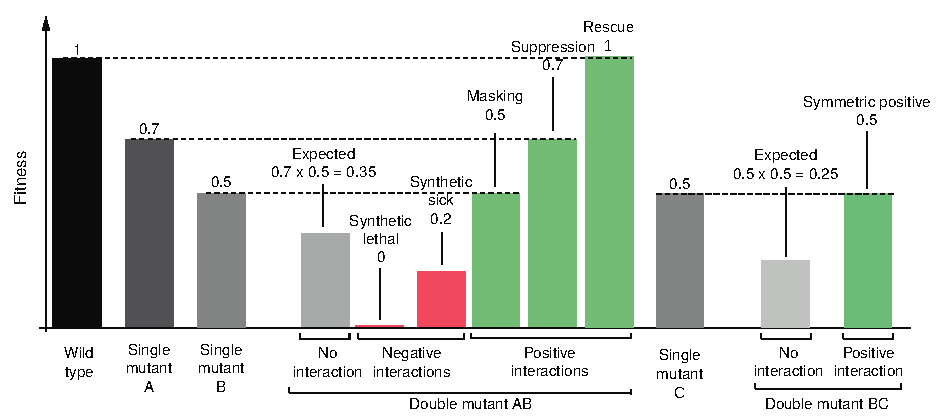
\includegraphics{Costanzo_2011_SL_mega_no_border.pdf}
    }
   \caption[Synthetic genetic interactions]{\textbf{Synthetic genetic interactions.} Impact of various negative and positive SGIs: negative interactions involve deleterious (sick) or inviable (lethal) phenotypess whereas positive interactions involve restoring viability by masking or suppressing the other mutation or complete rescue of the wildtype phenotype. Figure adapted from \citep{Costanzo2011} concerning growth viability fitness in yeast.}
\label{fig:Costanzo2011}
\end{figure}

\subsection{Synthetic Lethal Concepts in Genetics}

Synthetic lethal genes are generally regarded to arise due to functional redundancy. Due to the functional level of SGIs, synthetic lethal genes do not need directly interact, nor be expressed in the same cell or at the same developmental stage: serving related functions is sufficient to affect cell (or organism) viability and be relevant to drug-mode-of-action cancer biology. Combined loss of genes performing an essential or important function in a cell are therefore deleterious. Synthetic lethal gene pairs are therefore pairwise essential with ``induced essentiality'': each synthetic lethal gene becomes essential to the cell upon loss of the other.

Since synthetic lethal gene partners can be affected by extracellular stimuli and chemical, essentiality of synthetic lethal genes can be induced by the environment of a cell.  An environmental stress conditions may inhibit one or the other synthetic lethal gene, such as exposure to chemicals, in which case the synthetic lethal partner gene is ``conditionally essential'' \citep{Hillenmeyer2008}. Thus the evolutionary rationale for the abundance of SGIs (compared to the surprisingly low number of essential genes) in a Eukaryotic genome attributed to genetic functional redundancy and network robustness of a cell which are advantageous to survival. 

Biological functions are typically performed by a pathway of genes (or their products), may genes of the same pathway may be interchangable as synthetic lethal partners of a particular gene since loss of the pathway is deleterious without the synthetic lethal partner gene. Therefore biological pathways can be subject to induced essentiality under loss of a gene and synthetic lethality be defined occur at pathway level or occur in a gene regulation network. 

\subsection{Studies of Synthetic Lethality}
Genetic high-throughput screens have identified unexpected, functionally informative, and clinically relevant synthetic lethal interactions; including synthetic lethal partners of genes recurrently mutated in cancer or attributed to familial early-onset cancers. While screening presents an appealing strategy for synthetic lethal discovery, computational approaches are becoming popular as an alternative or complement to experimental methods to overcome inherent bias and limitations of experimental screens. An array of recently developed computational methods \citep{Wang2013, Tiong2014, Jerby2014, Lu2015, Wappett2014} show the need for synthetic lethal discovery in the fundamental genetics and translational cancer research community. However, existing computational methods are not suitable for queries of genomic data for interacting partners of a particular gene: they have been applied pairwise across the genome, do not have software released to apply the methodology, or lack statistical measures of error for further analysis. A robust prediction of gene interactions is an effective and practical approach at a scale of the entire genome for ideal translational applications, analysis of biological systems, and constructing functional gene networks.

\subsubsection{Synthetic Lethal Pathways and Networks}
SGIs are very common in genomes, with a 4$\times$ more interactions detected with synthetic gene array mating screens than protein-protein interactions yeast-2-hybrid studies \citep{Tong2004}. The SGI network is scale-free with power-law vertex degree distribution and low average shortest path length (3.3) as expected for a complex biological network \citep{Barabasi2004}. Highly connected ``hub'' genes with the highest number of links (vertex degree) are functionally important with many negative SGI hubs involved in cell cycle regulation and many positive SGI hubs involved in translation \citep{Baryshnikova2010b, Costanzo2010}. Negative SGIs were far more common than positive SGIs, with synthetic gene loss being more likely to be deleterious to cell than advantageous which indicates than synthetic lethality may be comparably easier to detect than other SGIs. 

Essential pathways are highly buffered with 5$\times$ more interactions than other SGIs, consistent with strong selection for survival, as found with conditional and partial mutations in essential genes \citep{Davierwala2005}. This SGI network had scale-free topology and rarely shared interactions with the protein-protein interaction network. These networks are related by an ``orthogonal'' relationship: shared partners in one network tend to be themselves connected directly in the other network. Essential genes were likely to have closely related functions, whereas non-essential networks more relatively more inclined to have SGIs between distinct biological pathways. 

\subsubsubsection{Conservation and Evolution of Synthetic Lethality}
There is poor conservation of specific SGIs between \textit{S. cerevisiae} and \textit{S. pombe} with 29\% of the interactions tested in both distantly related species being conserved between them (Dixon2008). The remaining interactions show high species-specific differences; however, many of the species specific interactions were still conserved between biological pathways, protein complexes, or protein-protein interaction modules. Similarly, conservation of pathway redundancy was also found between  Eukaryotes (\textit{S. cerevisiae}) and prokaryotes (\textit{E. coli}) \citep{Butland2008}. Negative SGIs were more likely to be conserved between biological pathways, whereas positive SGIs were more likely to be conserved within a pathway or protein complex \citep{Roguev2008}. 

A modest 5\% of interactions were conserved between unicellular (\textit{S. cerevisiae}) and multicellular (\textit{C. elegans}) organaisms but the nematode SGI network had similar scale-free topology and modularity despite difficulties metazoan RNAi screens being incomplete knockouts compared to null mutations in yeast \citep{Bussey2006}. The nematode SGI screen identified network hubs with important interactions to orthologues of known human disease genes \citep{Lehner2006}. Despite the lack of direct conservation of SGIs between yeasts and nematode worms, genetic redundancy at the gene or pathway level may yet be consistent with an induced essentiality model of SGIs where gene functions are conserved with network restructuring over evolutionary change \citep{Tischler2008}. While nematode models are more closely related to human cells, cancer cells can present growth and viability phenotypes more comparable to yeast models. Therefore findings from both SGA and RNAi models are relevant to understanding cellular network structure and in healthy and cancerous human cells. RNAi has also been applied to human and mouse cancer cells in cell culture and genetic screening experiments. These findsings suggest that SGI network ``rewiring'' is a concern for identifying specific synthetic lethal interactions in cancer and a pathway approach may be more robust in the context of evolution, patient variation, tumour heterogeneity, and disease progression.  

\subsection{Synthetic Lethal Concepts in Cancer}

Loss of function occurs in many genes in cancers including tumour suppressors and yet few interventions target such mutations compared to targeted therapies for gain of function mutation in oncogenes \citep{Kaelin2005}. Synthetic lethality is a powerful design strategy for therapies selective against loss of gene function with potential for application against a range of genes and diseases \citep{Kaelin2009, Fece2015}. Since synthetic lethality affects cellular viability by indirect functional relationships genes, it is suitable for indirectly targeting of muations in cancers. Once synthetic lethal partners of cancer genes are identified, targeted therapeutics can be applied against them. When genes are disrupted in cancers, the induced essentiality of synthetic lethal partners is a vulnerability that may be exploited for anti-cancer therapy. This has the potential to be very specific against cancer cells (with the target mutation) over non-cancer cells (with a functional compensating gene). Analogous to ``oncogene addiction'', where cances cells adapt to particular oncogenic growth signals and become reliant on them to remain viable \citep{Luo2009, Weinstein2000}, synthetic lethal partners of inactivated tumour suppressors are required to maintain cancer cell viability and proliferation as such they are subject to ``non-oncogene addiction'' and are feasible anti-cancer drug targets. 


\begin{figure}[!ht]
   \centering
   \resizebox{0.75 \textwidth}{!}{
    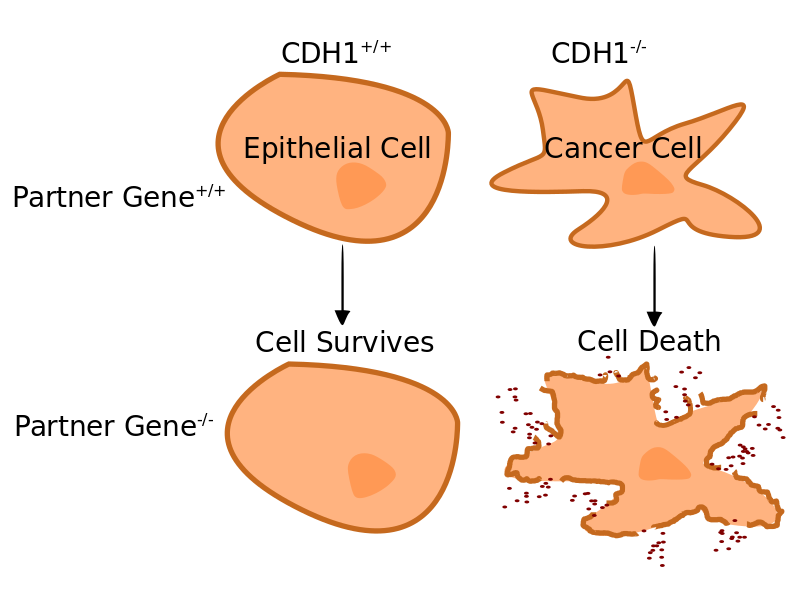
\includegraphics{SL_Concept_no_border.png}
   }
      \caption[Synthetic lethality in cancer]{\textbf{Synthetic lethality in cancer.} Rationale of exploiting synthetic lethality for specifity against a tumour suppressor gene (e.g.,  \textit{CDH1}) while other cells are spared under the inhibition of an SL partner gene.}
\label{fig:SL_Concept}
\end{figure}

The synthetic lethal approach to cancer medicine is most amenable to loss of function mutations in tumour suppressor genes, where it would feasibly be effective against any loss of function mutation across the tumour suppressor with a viable synthetic lethal partner gene (as shown in Figure \ref{fig:SL_Concept}). However, the approach may also be suitable for cases where cancer cells have mutations where the normal function of the gene is disrupted such as if it were overexpression (``synthetic dosage lethality'') or if an oncogene interfered with the function of the proto-oncogenic variant such as competitive inhibition. Thus synthetic lethality expands the range of cancer-specific mutations feasible to target with targeted therapeutics to absence of tumour suppressor genes and distinguishing highly homologous oncogenes by functional differences by targeting their synthetic lethal partners. 

\subsection{Clinical Impact of Synthetic Lethality in Cancer}

%Targeted therapeutics combined with the adoption of genomics to identify mutations have begun to impact upon the clinical treatment of cancers. Early examples of targeted therapies are strikingly effective, such as vemurafenib which has shown promise against \textit{BRAF}(V600E) mutations in melanomas in clinical trials \citep{Ravnan2012} and may be widely applicable despite issues with genetic background and drug resistance \citep{Sun2014,Prahallad2012}. Meanwhile, synthetic lethal drug design to indirectly target inactivated genes in cancer has the potential to drastically accelerate the development of precision cancer medicine \citep{Kaelin2009}.

%Synthetic lethal interaction between \textit{\textit{PARP1}} and the tumour suppressor genes \textit{\textit{BRCA1}} and \textit{\textit{BRCA2}} has been demonstrated in cell line and mouse xenograft models, with promising results in both RNAi and drug inhibition experiments \citep{Bryant2005,Farmer2005}. These interactions have been shown to be clinically relevant, with the \textit{\textit{PARP1}}-targeting drug olaparib exhibiting success in clinical trials involving germline and sporadic \textit{\textit{BRCA1}} or \textit{\textit{BRCA2}} mutations in both breast and ovarian cancers, and resulting in fewer adverse effects than cytotoxic chemotherapy \citep{Tutt2010,Audeh2010}. \textit{\textit{PARP1}} inhibitors have shown anti-cancer activity against mutations in other DNA repair genes such as \textit{PTEN} and have been proposed for chemopreventative applications as an alternative to prophylactic surgery for high risk individuals with germline \textit{BRCA1} or \textit{BRCA2} mutations \citep{Strom2012}. Complications were observed in clinical trials, such as acquired drug resistance, complex modifier interactions with \textit{\textit{PARP1}} inhibitors, and their application integrated with genetic tests across cancers in multiple tissues (most commonly breast and ovarian) \citep{Lord2014}. 

The synthetic lethal interaction of \textit{BRCA1} or \textit{BRCA2} with \textit{PARP1} in breast cancer is an example of how gene interactions are important in cancer, including translation to the clinic. These genetic interactions enable specific targeting of mutations in \textit{BRCA1} or \textit{BRCA2} tumour suppressor genes with PARP inhibitors by inducing synthetic lethality in breast cancer \citep{Farmer2005}. PARP inhibitors are one of the first targeted therapeutics against a tumour suppressor mutation with success in clinical trials. 

\textit{BRCA1} or \textit{BRCA2} and \textit{PARP1} genes demonstrate the application of the synthetic lethal approach to cancer therapy \citet{Ashworth2008, Kaelin2005}. \textit{BRCA1} and \textit{BRCA2} are homologous DNA repair genes, widely known as tumour suppressors; mutation carriers have substantially increased risk of breast (risk by age 70 of 57\% for \textit{BRCA1} and 59\% for \textit{BRCA2}) and ovarian cancers (risk by age 70 of 40\% for \textit{BRCA1} and 18\% for \textit{BRCA2}) \citep{Chen2007}. The \textit{BRCA1} or \textit{BRCA2} genes, which usually repair DNA or destroy the cell if it cannot be repaired, have inactivating somatic mutations in some familial and sporadic cancers. Poly-ADP-ribose polymerase (PARP) genes are tumour suppressor genes involved in base excision DNA repair. Loss of PARP activity results in single-stranded DNA breaks. However, \textit{PARP1}\textsuperscript{-/-} knockout mice are viable and healthy indicating low toxicity from PARP inhibition \citep{Bryant2005}.  

\citet{Bryant2005} showed that \textit{BRCA2}\textsuperscript{{}-/-} cells were sensitive to PARP inhibition by siRNA of \textit{PARP1} or drug inhibition (which targets \textit{PARP1} and \textit{PARP2}) using Chinese hamster ovary cells, MCF7 and MDA-MB-231 breast cell lines. This effect was sufficient to kill mouse tumour xenografts and showed high specificity to \textit{BRCA2} deficient cells in culture and xenografts. \citet{Farmer2005} replicated these results in embryonic stem cells and showed that \textit{BRCA1}\textsuperscript{{}-/-} cells were also sensitive to PARP inhibition relative to the wild-type with siRNA and drug experiments in cell culture and drug activity against \textit{BRCA1} or \textit{BRCA2} deficient embryonic stem cell mouse xenografts. They found evidence that PARP inhibition causes DNA lesions, usually repaired in wild-type cells, which lead to chromosomal instability, cell cycle arrest, and induction of apoptosis in \textit{BRCA1} or \textit{BRCA2} deficient cells. Therefore, the pathways cooperate to repair DNA giving a plausible mechanism for combined loss as an effective anti-cancer treatment.  

Thus PARP inhibitors have potential for clinical use against \textit{BRCA1} or \textit{BRCA2} mutations in hereditary and sporadic cancers (Ashworth 2008; Kaelin2005). PARP inhibition has been found to be effective in cancer patients carrying \textit{BRCA1} or \textit{BRCA2} mutations and some other ovarian cancers, suggesting synthetic lethality between PARP and other DNA repair pathways \citep{Strom2012}. This supports the potential for PARP inhibition as a chemo-preventative alternative to prophylactic surgery for high risk individuals with \textit{BRCA1} or \textit{BRCA2} mutations \citep{Strom2012}. Hormone-based therapy has also been suggested as a chemo-preventative in such high risk individuals and aromatase inhibitors have completed phase I clinical trials for this purpose (Bozovic-Spasojevic2012). \citet{Strom2012} also postulate increased efficacy of PARP inhibitors in the hypoxic DNA-damaging tumour micro-environment.  

A PARP inhibitor, olaparib, showed fewer adverse effects than cytotoxic chemotherapy and anti-tumour activity in phase I trials against \textit{BRCA1} or \textit{BRCA2} deficient familial breast, ovarian, and prostate cancers \citep{Fong2009} and sporadic ovarian cancer \citep{Fong2010}. AstraZeneca has reported phase II trials showing the treatment is effective in \textit{BRCA1} or \textit{BRCA2} deficient breast \citep{Tutt2010} and ovarian cancers \citep{Audeh2010} with a favourable therapeutic window and similar toxicity between carriers of \textit{BRCA1} or \textit{BRCA2} mutations and sporadic cases. AstraZeneca announced that olaparib has begun phase III trials for breast and ovarian cancers in 2013. Mixed results in phase II trials in ovarian cancer are behind the delays addressed by retrospective analysis of the cohort subgroup with confirmed mutation of \textit{BRCA1} or \textit{BRCA2} genes in the tumour; unsurprisingly these patients, benefit most from the PARP inhibitor treatment and have increased platinum sensitivity in combination treatment. This demonstrates the clinical impact of a well characterised system of synthetic lethality with known cancer risk genes. Synthetic lethality has the benefit of being effective against inactivation of tumour suppressor genes by any means, broader than targeting a particular oncogenic mutation \citep{Kaelin2005}. The targeted therapy is effective in both sporadic and hereditary \textit{BRCA1} or \textit{BRCA2} deficient tumours acting against an oncogenic molecular aberration across several tissues.  

[Update re. FDA approval for Ovarian]

These PARP inhibitors are FDA approved for some cancers \cite{McLachlan2016}, are effective against germline and sporadic \textit{BRCA1} or \textit{BRCA2} mutations, and are a potential preventation alternative to prophylactic surgery for high risk mutation carriers \cite{Strom2012}.


\subsection[High{}-throughput Screening for Synthetic Lethality]{High-throughput Screening for Synthetic Lethality}

%Candidate hypothesis driven synthetic lethal studies in cancer have been successful in some cases \citep{Farmer2005,Bryant2005,vanPel2013} but potentially meaningful synthetic lethal interactions can also occur between unexpected pathways and with genes involved in different biological functions \citep{Costanzo2011}. Unbiased screening is therefore an appealing strategy to identify synthetic lethal interactions, including those informative of novel biological functions, drug mode-of-action, or amenable to treatment. Current screening in cancer cell lines uses genetic or pharmacological approaches, with RNAi or compound libraries respectively, to discover synthetic lethal interactions \citep{Fece2015}.

%Genetic screens can facilitate the discovery of specific genes interacting with a particular disease gene, identify biomarkers for treatment response, and inform development of targeted therapies (with a known mode-of-action and anticipated mechanisms of resistance). Synthetic lethal screens using RNAi have been applied to many cancer genes in cell line models including \textit{\textit{VHL}} in renal cancer \citep{Jerby2014}, \textit{\textit{FH}} in renal cancer \citep{Boettcher2014}, \textit{\textit{WEE1}} in colorectal cancer \citep{Aarts2015}, and \textit{CDH1} in breast cancer \citep{Telford2015}. While some candidates identified in these screens are consistent with the literature or were successfully validated, RNAi screens are susceptible to false positives and a large number of interaction candidates have not been tested, validated, or replicated \citep{Lu2015,Jerby2014,Boettcher2014,Azorsa2009}.

%Chemical screens are a complementary approach that can be used to screen for compounds effective against a particular mutation. While these identify lead compounds with specific activity against mutants, such screens do not ensure compounds are bioavailable, have known mode-of-action, or are selective against a particular target gene and key drug classes are not tested \citep{Fece2015,Kaelin2005,Chan2011}. Despite this, synthetic lethal screens have become widely used for functional genomics and translational  research to identify potential targets for drug development \citep{Fece2015,Telford2015,Jerby2014,Boettcher2014,vanderMeer2014}.

%relevance?
%%%%%%%%%%%
%Genomic and pharmacological screens are becoming widely used for biomedical research despite many potential sources of error \citep{Fece2015,Kaelin2009,Chan2011}.  Off-target effects \citep{Kaelin2005,Chan2011,Fece2015} and growth inhibition \citep{Diehl2014}, from delivery of potentially selective agents, is an issue with RNAi experiments screening for differential viability between cell lines or treatment conditions such as synthetic lethal screens. Mechanisms of gene inhibition, particularly transient gene knockdown in RNAi screens, differ considerably from the behaviour inhibitors in the clinic \citep{Kaelin2009}. Screens are biased  towards genes which are amenable to inhibition, particularly chemical screens which are over-represented for gene functions with existing drugs inhibitors \citep{Chan2011}. Mutations, RNA knockdown, and drug inhibition have different effects on gene function, so perhaps unsurprisingly, synthetic lethal interactions often fail to replicate across experimental systems, cell lines, tissue types, or species \citep{Kaelin2009,Dixon2009}. Several alternatives have been raised to overcome some of these shortcomings of synthetic lethal screens including genome-wide screens with episomal gene transfer \citep{Chan2011}, lentiviral RNAi \citep{Diehl2014}, or CRISPR/\textit{Cas9} genome editing \citep{Fece2015,Shalem2015,Hart2015,Thompson2015}. However, these do not preclude the possibility of off-target effects or account for diverse genetic backgrounds or tumour heterogeneity \citep{Fece2015}.
%%%%%%%%%%%%
%% to consider (here or discussion): off-targets (even with newer tech), differences in KO mechanism -> effect, lack of reproducibility/validations of candidates


The function of signalling pathways and combinations of interacting genes are important in cancer research but classical genetics approaches have been limited to non-redundant pathways \citep{Fraser2004}. The emerging RNAi technologies have vastly expanded the potential for studying genetic redundancy in mammalian experimental models including testing experimentally for synthetic lethality \citep{Fraser2004}. Identifying synthetic lethality is crucial to study gene function, drug mechanisms, and design novel therapies \citep{Lum2004}. Candidate selection of synthetic lethal gene pairs relevant to cancer has shown some success but is limited because interactions are difficult to predict; they can occur between seemingly unrelated pathways in model organisms \citep{Costanzo2011}. While biologically informed hypotheses have had some success in synthetic lethal discovery \citep{Bitler2015, Bryant2005, Farmer2005}, interactions occurring indirectly between distinct pathways would be missed \citep{Boone2007, Costanzo2011}. Scanning the entire genome for interactions against a clinically relevant gene is an emerging strategy being explored with high-throughput screens \citep{Fece2015} and computational approaches \citep{Boucher2013, vanSteen2011}.  

Experimental screening for synthetic lethality is an appealing strategy for wider discovery of functional interactions \textit{in vivo} despite many potential sources of error which must be considered. The synthetic lethal concept has both genetic and pharmacological screening applications to cancer research. Genetic screens, with RNAi to discover the specific genes involved, inform development of targeted therapies with a known mode of action, anticipated mechanisms of resistance, and biomarkers for treatment response. RNAi is a transient knockdown of gene expression more similar to the effect of drugs than complete gene loss and makes comparison to screens in model organisms difficult \citep{Bussey2006}. The RNAi gene knockdown process has inherent toxicity to some cells, potential off-target effects, and issues with a high false positive rate. Therefore, it is important to validate any candidates in a secondary screen and replicate knockdown experiments with a number of independent shRNAs. Alternative gene knockout procedures have also been proposed for synthetic lethal screening including a genome-wide application of the CRIPR/Cas9/sgRNA genome editing technology \citep{Sander2014}, episomal gene transfer \citep{Vargas2004}, or RNAi with lentiviral transfection for delivery of shRNA \citep{Telford2015}. Genetic screens have potential for quantitative gene disruption experiments to selectively target overexpressed genes in cancer via synthetic dosage lethality. While powerful for understanding fundamental cellular function, analysis of isogenic cell lines is inherently limited by assuming only a single mutation differs between them despite susceptibility to ``genetic drift'' and cannot account for diverse genetic backgrounds or tumour heterogeneity \citep{Fece2015}. Genetic screens thus identify targets to develop or repurpose targeted therapies for disease but alone will not directly identify a lead compound to develop for the market or clinical translation.  

Chemical screens are immediately applicable to the clinic by directly screening for selective lead compounds with suitable pharmacological properties. However chemical screens lack a known mode of action, may affect many targets, and screen a narrow range of genes with existing drugs. With either approach there are many challenges translating candidates into the clinic such as finding targets relevant to a range of patients, validation of targets, accounting for a range of genetic (and epigenetic) contexts or tumour micro-environment, identifying effective synergistic combinations, enhancers of existing radiation or cytotoxic treatments, avoiding inherent or acquired drug resistance, and developing biomarkers for patients which will respond to synthetic lethal treatment, including integrating these into clinical trials and clinical practice. Identifying specific target genes is an effective way to anticipate such challenges, which can be approached with genetic screens, so we will focus on these and computational alternatives. Screening methods have proven a fruitful area of research, despite being costly, laborious, and having many different sources of error. These limitations suggest a need for complementary computational approaches to synthetic lethal discovery.  

\subsubsection{Examples of Synthetic Lethal Screens}

Overexpression of genes is another suitable application for synthetic lethality since overexpressed genes cannot be distinguished from the wild-type by direct sequence specific targeted therapy. Overexpression of oncogenes, such as \textit{EGFR}, \textit{MYC}, and \textit{PIM1}, has been found to drive many cancers. \textit{PIM1} is a candidate for synthetic lethal drug design in lymphomas and prostate cancers, where it interacts with \textit{MYC} to drive cancer growth. \citet{vanderMeer2014} performed an RNAi screen to for synthetic lethality between \textit{PIM1} overexpression and gene knockdown in RWPE prostate cancer cell lines. \textit{PLK1} gene knockdown and drug inhibition was an effective as a specific inhibitor of \textit{PIM1} overexpressing prostate cells in cell culture and mouse tumour xenografts. \textit{PLK1} inhibition reduced \textit{MYC} expression in pre-clinical models, consistent with expression in human tumours which \textit{PIM1} and \textit{PLK1} are co-expressed and correlated with tumour grade. Thus RNAi screening was valuable to identify a therapeutic targets and biomarkers for patient response as demonstrated with the finding of \textit{PLK1} as a candidate drug target against prostate cancer progression.  

Hereditary leiomyomatosis and renal cell carcinoma (HLRCC) is a cancer syndrome of predisposition to benign tumours in the uterus and risk of malignant cancer of the kidney attributed to inherited mutations in fumarate hydratase (\textit{FH}). \citet{Boettcher2014} performed an RNAi screen on HEK293T renal cells for synthetic lethality with \textit{FH}. They found enrichment of haem metabolism (consistent with the literature) and adenylate cyclase pathways (consistent with cAMP dysregulation in \textit{FH} mutant cells). Synthetic lethality between \textit{FH} mutation and adenylate cyclases was validated with gene knockdown, drug experiments, and replicated across both HEK293T renal cells and VOK262 cells derived from a HLRCC patient, suggesting new potential treatments against the disease. %Therefore, synthetic lethality is applicable to metabolic dysregulation in cancer, consistent with the Warburg hypothesis (Warburg 1956), and successfully identifies specific anti-cancer drugs, even when the mechanism is unclear. 

Similarly, hereditary diffuse gastric cancer (HDGC) is a cancer syndrome of predisposition to early-onset malignant stomach and breast cancers attributed to mutations in E-cadherin (\textit{CDH1}). \citet{Telford2015} performed an RNAi screen on MCF10A breast cells for synthetic lethality with \textit{CDH1}. They found enrichment of G-protein coupled receptors (GPCRs) and cytoskeletal gene functions. The results were consistent with a concurrent drug compound screen with a number of candidates validated by lentiviral shRNA gene knockdown and drug testing including inhibitors of Janus kinase, histone deacetylases, phosphoinositide 3-kinase, aurora kinase, and tyrosine kinases. Therefore the synthetic lethal strategy has potential for clinical impact against HDGC, with particular interest in interventions with low adverse effects for chemo-prevention, including repurposing existing approved drugs for activity against \textit{CDH1} deficient cancers.  

RNAi screening for synthetic lethality is also useful for functional genetics to understand drug sensitivity. \citet{Aarts2015} screened WiDr colorectal cells for synthetic lethality between \textit{WEE1} inhibitor treatment and an RNAi library of 1206 genes with functions known to be amenable to drug treatment or important in cancer such as kinases, phosphatases, tumour suppressors, and DNA repair (a pathway \textit{WEE1} regulates). Screening identified a number of synthetic lethal candidates including genes involved in cell cycle regulation, DNA replication, repair, homologous recombination, and Fanconi anaemia. Synthetic lethality with cell-cycle and DNA repair genes was consistent with the literature and validation in a panel of breast and colorectal cell lines supported checkpoint kinases, Fanconi anaemia, and homologous recombination as synthetic lethal partners of \textit{WEE1}. These results show that synthetic lethality can be used to improve drug sensitivity as a combination treatment, especially to exploit genomic instability and DNA repair, which are known to be clinically applicable from previous results with \textit{BRCA1} or \textit{BRCA2} genes and PARP inhibitors \citep{Lord2014}. Therefore, \textit{WEE1} inhibitors are an example of treatment which could be repurposed with the synthetic lethal strategy and similar findings would be valuable to clinicians as a source of biomarkers and novel treatments. While using a panel of cell lines to replicate findings across genetic background is a promising approach to ensure wide clinical application of validated synthetic lethal partners, a computational approach may be more effective as it could account for wider patient variation than scaling up intensive experiments on a wide array of cell lines and could screen beyond limited candidates from an RNAi library.  

Chemical genetic screens are also a viable strategy to identify therapeutically relevant synthetic lethal interactions. \citet{Bitler2015} investigated \textit{ARID1A} mutations, aberrations in chromatin remodelling known to be common in ovarian cancers, for drug response. Ovarian RMG1 cells were screened for drug response specific to \textit{ARID1A} knockdown cells. They used \textit{ARID1A} gene knockdown for consistent genetic background, with control experiments and 3D cell culture to ensure relevance to drug activity in the tumour micro-environment. Screening a panel of commercially available drugs targeting epigenetic regulators found \textit{ESH2} methyltransferase inhibitors effective and specific against \textit{ARID1A} mutation with validation in a panel of ovarian cell lines. Synthetic lethality between \textit{ARID1A} and \textit{ESH2} was supported by decreases in H3K27Me3 epigenetic marks and markers of apoptosis in response to \textit{ESH2} inhibitors. This was mechanistically supported with differential expression of \textit{PIK3IP1} and association of both synthetic lethal genes with the \textit{PIK3IP1} promoter identifying the PI3K-AKT signalling pathway as disrupted when both genes are inhibited. This successfully demonstrates the importance of synthetic lethality in epigenetic regulators, identifies a therapeutically relevant synthetic lethal interaction, and shows that chemical genetic screens could model drug response and combination therapy in cancer cells. However this approach is limited to finding synthetic lethal interactions between genes with known similar function, which may not be the most suitable for treatment. Further limiting experiments to genes with existing targeted drugs reduces the number of synthetic lethal interactions detected, assumes on their drug specificity to a particular target, and many of these drugs are not clinically available yet anyway as they are still in clinical trials for other diseases or are not supported by healthcare systems in many countries.  

The examples above show that high-throughput screens are an effective approach to discover synthetic lethality in cancer with a wide range of applications. Screens are more comprehensive than hypothesis-driven candidate gene approaches and successfully find known and novel synthetic lethal interactions with potential for rapid clinical application. They have the power to test mode of action of drugs, find unexpected synthetic lethal interactions between pathways, or identify effective treatment strategies without needing a clear mechanism. However, synthetic lethal screens are costly, labour-intensive, error-prone, and biased towards genes with effective RNAi knockdown libraries. Limited genetic background, lethality to wild-type cell during gene knockdown, off-target effects, and difficultly replicating synthetic lethality across different cell lines, tissues, laboratories, or conditions stems from a high false positive rate and a lack of standardised thresholds to identify synthetic lethality in a high-throughput screen. Therefore there is a need for replication, validation, and alternative approaches to identify synthetic lethal candidates. Varied conditions between experimental screens and differences between RNAi or drug screens makes meta-analysis difficult. Thus genome-scale synthetic lethal experiments are not feasible, even in model organisms, so a computational approach would be more suitable for this task.  

\subsection[Computational Prediction of Synthetic Lethality]{Computational Prediction of Synthetic Lethality}

%Computational approaches to identifying synthetic lethal interactions are rapidly developing into a feasible addition to genomic screens due to the low cost, reliable automated reproducible workflows, ability to account for distinct genetic backgrounds, and lack of off-target effects or bias towards particular genes \citep{Boucher2013, Thompson2015}. 
%%%%%%%%relevance
%Synthetic lethal prediction has been widely explored in model organisms - a key example is the task of inferring the entire gene network from incomplete synthetic lethal networks and functional genomics data in \textit{Saccharomyces cerevisiae} \citep{Boucher2013}. However, synthetic lethal interactions are difficult to reproduce across species \citep{Dixon2009,Lehner2006}, not all of the data types used for prediction of synthetic lethal interactions in available in humans, and the methods assuming conserved network structure may not be applicable to unstable cancer systems. Computational approaches to discovery of synthetic lethal interactions tailored to mammals, or specifically to human cancers, are therefore needed for applicable results. However, many existing computational approaches are difficult to apply to novel genes having been trained on known gene functions, using complex machine learning methods, or are over-represented for genes where single gene aberrations have large effects on cellular phenotypes such as \textit{\textit{TP53}} or \textit{AKT}.
%%%%%%% join to next subsubsubsection
%Analysis of gene expression is an appealing strategy for discovery of synthetic lethal interactions in cancer due to the widespread availability of data for different cancers, lack of bias towards well characterised genes, and potential further use for expression of interacting partners as biomarkers for treatment with drugs designed to exploit them.

%A recent example of a computational tool for identification of synthetic lethal interactions using gene expression analysis is the DAISY methodology \citep{Ryan2014,Crunkhorn2014}, which combines predictions from patient samples  of The Cancer Genome Atlas (TCGA), cell lines of the Cancer Cell Line Encyclopaedia (CCLE), and RNAi validation experiments \citep{Jerby2014}. The predictors of synthetic lethality were genomic `survival of the fittest' (using DNA copy number and somatic mutation in patient and cell lines data), `functional examination' of gene essentiality (using RNA interference data in cell cell lines), and pairwise `gene co-expression' (in cell lines).

%%%%%%%% edit to tone down anti-DAISY message  restructure subsubsubsections to fewer ideas apiece
%As a proof-of-concept, DAISY demonstrates the potential of bioinformatics approaches to generate synthetic lethal candidates against the tumour suppressor \textit{\textit{VHL}} in a renal cancer cell line, along with reasonable statistical performance and generalisation to gene essentiality, genetic dosage, or drug analyses \citep{Jerby2014}. However, DAISY partners of \textit{\textit{VHL}} showed only modest 4$\times$ over-represent\-ation in validated shRNA screening than a screen of random genes and the method has not been widely adopted in studies of other cancer genes.
%%criticism of DAISY moved to discussion

%An alternative to the approach is the use of `cancer genome evolution' to predict synthetic lethal genes from their behaviour in genomics data\citep{Lu2015}, as the induced essentiality of remaining synthetic lethal partners takes effect in the tumour progression. Lu \textit{et al.} \citep{Lu2015} postulate that, in response to loss of a gene function, a tumour would would either resist by maintaining low expression or compensate by increasing the activity of synthetic lethal partner genes. This model predicted far more genes than previous attempts at discovery of synthetic lethal interactions, performed well at a genome-wide scale, and produced a higher 14$\times$ over-represent\-ation of validated synthetic lethal pairs. While Lu \textit{et al.} \citep{Lu2015} provide a comprehensive list of their strongest candidate synthetic lethal pairs across cancer types, these do not include \textit{CDH1}, thus there remains a need for computational predictions for this gene and a tool other researchers may use for similar screen triage purposes against a candidate gene in a specific cancer.  


%% (Re)move the below subsubsubsection? Too negative / irrelevant?
%These prior approaches used complex cutting-edge machine learning techniques which may be difficult for the biological community to adopt and DNA copy number which may not be available for many  applications \citep{Jerby2014, Lu2015}. %% may be speculation
%Here, we present a synthetic lethal analysis based solely on gene expression data which could feasibly be applied to studies of other genes to utilise the large number of samples collected for many genes in diseases such as cancers.  We use the example of \textit{CDH1} as a tumour suppressor gene in breast cancer samples from TCGA \citep{TCGA2012} to highlight the importance of synthetic lethal interactions, potential relationships between them, and the biological pathways involved.
%R code for our synthetic lethal analysis will be avaialable on our \href{https://github.com/TomKellyGenetics/slipt}{GitHub repository} as an R package. 

\subsubsection{Bioinformatics approaches to gene interactions}

Prediction of gene interaction networks is a feasible alternative to high-throughput screening with biological importance and clinical relevance. There are many existing methods to predict gene networks, as reviewed by \citet{vanSteen2011} and \citet{Boucher2013} and summarised in Table \ref{tab:methods_model}. However, many of these methods have limitations including the requirement for existing SGI data, several data inputs, and reliability of gene function annotation. Many of the existing methods also assume conservation of individual interactions between species, which has been found not to hold in yeast studies \citep{Dixon2008}. Tissue specificity is important in gene regulation and gene expression, which are used as predictors of genetic interaction. However, tissue specific of genetic interactions cannot be explored in yeast studies and has not been considered in many studies of multicellular model organisms, human networks, or cancers. Similarly, investigation into tissue specific of protein-protein interactions (PPIs) , an important predictor of genetic interactions, is difficult given the high-throughput two-hybrid screens occur out of cellular context for multicellular organisms.  

\begin{table}[!ht]
\caption{Methods for Predicting Genetic Interactions}
\label{tab:methods_model}
\makebox[\textwidth][c]{
\resizebox{1.15 \textwidth}{!}{
%\setlength\LTleft{0pt}
%\setlength\LTright{0pt}
\begin{tabular}{l|l|l|l|l}

\multicolumn{1}{l}{\textbf{Method}} &
\multicolumn{1}{l}{\textbf{Input Data}} &
\multicolumn{1}{l}{\textbf{Species}} &
\multicolumn{1}{l}{\textbf{Source}} &
\multicolumn{1}{l}{\textbf{Tool Offered}} \\ \hline
\cellcolor[rgb]{0.8509804,0.8862745,0.9529412}\color{black}
\textcolor{black}{Between Pathways Model} &
\cellcolor[rgb]{0.8509804,0.8862745,0.9529412}\color{black} PPI, SGI &
\cellcolor[rgb]{0.8509804,0.8862745,0.9529412}\color{black}
\textit{\textcolor{black}{S. cerevisiae}} &
\cellcolor[rgb]{0.8509804,0.8862745,0.9529412}\color{black}
\citet{Kelley2005} &
\cellcolor[rgb]{0.8509804,0.8862745,0.9529412}~
\\\hline
Within Pathways Model &
PPI, SGI &
\textit{S. cerevisiae} &
\citet{Kelley2005} &
~
\\\hline
\cellcolor[rgb]{0.8509804,0.8862745,0.9529412}\color{black}
\textcolor{black}{Decision Tree} &
\cellcolor[rgb]{0.8509804,0.8862745,0.9529412}\color{black} PPI,
expression, phenotype &
\cellcolor[rgb]{0.8509804,0.8862745,0.9529412}\color{black}
\textit{\textcolor{black}{S. cerevisiae}} &
\cellcolor[rgb]{0.8509804,0.8862745,0.9529412}\color{black}
\citet{Wong2004} &
\cellcolor[rgb]{0.8509804,0.8862745,0.9529412}\color{black} 2
Hop\\\hline
Logistic Regression &
SGI, PPI, co-expression, phenotype &
\textit{C. elegans} &
\cite{Zhong2006} &
Gene Orienteer\\\hline
\cellcolor[rgb]{0.8509804,0.8862745,0.9529412}\color{black}
\textcolor{black}{Network Sampling} &
\cellcolor[rgb]{0.8509804,0.8862745,0.9529412}\color{black} SGI, PPI, GO
&
\cellcolor[rgb]{0.8509804,0.8862745,0.9529412}\color{black}
\textit{\textcolor{black}{S. cerevisiae}} &
\cellcolor[rgb]{0.8509804,0.8862745,0.9529412}{
\begin{tabular}{@{\hskip0pt}l@{\hskip0pt}}\color{black}\citet{LeMeur2008} \\ \color{black}\citet{LeMeur2014}\end{tabular}}
&
\cellcolor[rgb]{0.8509804,0.8862745,0.9529412}\color{black}
SLGI(R)\\\hline
Random Walk &
GO, PPI, expression &

\begin{tabular}{@{\hskip0pt}l@{\hskip0pt}}\textit{S. cerevisiae} \\ \textit{C. elegans}\end{tabular}
 &
\citet{Chipman2009} &
~
\\\hline
\cellcolor[rgb]{0.8509804,0.8862745,0.9529412}\color{black}
\textcolor{black}{Shared Function} &
\cellcolor[rgb]{0.8509804,0.8862745,0.9529412}\color{black}
Co-expression, PPI, text mining, phylogeny &
\cellcolor[rgb]{0.8509804,0.8862745,0.9529412}\color{black}
\textit{\textcolor{black}{C. elegans}} &
\cellcolor[rgb]{0.8509804,0.8862745,0.9529412}\color{black}
\citet{Lee2010b} &
\cellcolor[rgb]{0.8509804,0.8862745,0.9529412}\color{black}
WormNet\\\hline
Logistic Regression &
Co-expression, PPI, phenotype &
\textit{C. elegans} &
\citet{Lee2010a} &
GI Finder\\\hline
\cellcolor[rgb]{0.8509804,0.8862745,0.9529412}\color{black}
\textcolor{black}{Jaccard Index} &
\cellcolor[rgb]{0.8509804,0.8862745,0.9529412}\color{black} GO, SGI,
PPI, phenotype &
\cellcolor[rgb]{0.8509804,0.8862745,0.9529412}\color{black} Eukarya &
\cellcolor[rgb]{0.8509804,0.8862745,0.9529412}\color{black}
\citet{Hoehndorf2013} &
\cellcolor[rgb]{0.8509804,0.8862745,0.9529412}~
\\\hline
\iffalse
Bimodal Statistics &
~
 &
~
 &
\cite{Wappett2014} &
BiSEp(R)\\\hline
\cellcolor[rgb]{0.8509804,0.8862745,0.9529412}\color{black}
\textcolor{black}{Machine Learning} &
\cellcolor[rgb]{0.8509804,0.8862745,0.9529412}~
 &
\cellcolor[rgb]{0.8509804,0.8862745,0.9529412}~
 &
\cellcolor[rgb]{0.8509804,0.8862745,0.9529412}
\begin{tabular}{@{\hskip0pt}l@{\hskip0pt}}\color{black} Discussed by \citep{Babyak2004} \\and \citet{Lee2009} \end{tabular}

 &
\cellcolor[rgb]{0.8509804,0.8862745,0.9529412}~
\\\hline
\begin{tabular}{@{\hskip0pt}l@{\hskip0pt}}\color{black} Machine Learning \\as discussed by \citet{Wu2014}  \end{tabular}
&
~
 &
~
 &

\begin{tabular}{@{\hskip0pt}l@{\hskip0pt}}
\citet{Qi2008} \\
\citet{Paladugu2008} \\
\citet{Li2011}
\end{tabular}
&
~
\\\hline
\fi
\cellcolor[rgb]{1, 1, 1}\color{black}
\textcolor{black}{Machine Learning} &
\cellcolor[rgb]{1, 1, 1}~
 &
\cellcolor[rgb]{1, 1, 1}~
 &
\cellcolor[rgb]{1, 1, 1}\color{black}
\citet{Pandey2010} &
\cellcolor[rgb]{1, 1, 1}\color{black} MNMC\\\hline
\rowcolor[rgb]{0.8509804,0.8862745,0.9529412}
Machine Learning Meta-Analysis &
~
 &
~
 &
\cite{Wu2014} &
MetaSL\\\hline
\cellcolor[rgb]{1, 1, 1}{\color{black}
\begin{tabular}{@{\hskip0pt}l@{\hskip0pt}}
\textcolor{black}{Flux Variability Analysis} \\
\textcolor{black}{Flux Balance Analysis} \\
\textcolor{black}{Network Simulation}
\end{tabular}
} &
\cellcolor[rgb]{1, 1, 1}\color{black} Metabolism &
\cellcolor[rgb]{1, 1, 1}{\color{black}

\begin{tabular}{@{\hskip0pt}l@{\hskip0pt}}
\textit{\textcolor{black}{E. coli}} \\
\color{black} \textit{\textcolor{black}{Mycoplasma pneumoniae}}
\end{tabular}
} &
\cellcolor[rgb]{1, 1, 1}\color{black}
\citet{Guell2014} &
\cellcolor[rgb]{1, 1, 1}~
\\\hline
\end{tabular}
}
}
\end{table}

\begin{table*}[!ht]
\caption{Methods for Predicting Synthetic Lethality in Cancer}
\label{tab:methods_SL}
%\begin{center}
\resizebox{ \textwidth}{!}{
\begin{tabular}{l|l|l|l}
\multicolumn{1}{m{4.421cm}}{\cellcolor{white}\bfseries\color{black}
Method} &
\multicolumn{1}{m{2.342cm}}{\cellcolor{white}\bfseries\color{black}
\textcolor{black}{Input Data}} &
\multicolumn{1}{m{4.552cm}}{\cellcolor{white}\bfseries\color{black}
Source} &
\cellcolor{white}\bfseries\color{black} Tool Offered\\\hline
\cellcolor[rgb]{0.8509804,0.8862745,0.9529412}\color{black}
\textcolor{black}{Network Centrality} &
\cellcolor[rgb]{0.8509804,0.8862745,0.9529412}\color{black} protein-protein interactions &
\cellcolor[rgb]{0.8509804,0.8862745,0.9529412}\color{black}
\citet{Kranthi2013} &
\cellcolor[rgb]{0.8509804,0.8862745,0.9529412}~
\\\hline
Differential Expression &
\begin{tabular}{@{\hskip0pt}l@{\hskip0pt}}
Expression \\
Mutation
\end{tabular}
&
\citet{Wang2013} &
~
\\\hline
\cellcolor[rgb]{0.8509804,0.8862745,0.9529412}{\color{black}

\begin{tabular}{@{\hskip0pt}l@{\hskip0pt}}
\textcolor{black}{Comparative Genomics} \\
\color{black} \textcolor{black}{Chemical-Genomics}
\end{tabular}
}
 &
\cellcolor[rgb]{0.8509804,0.8862745,0.9529412}

\begin{tabular}{@{\hskip0pt}l@{\hskip0pt}}
Yeast synthetic gene interactions\\
Homology
\end{tabular}
 &
\cellcolor[rgb]{0.8509804,0.8862745,0.9529412}\color{black}
\citet{Heiskanen2012} &
\cellcolor[rgb]{0.8509804,0.8862745,0.9529412}~
\\\hline
Comparative Genomics &
\begin{tabular}{@{\hskip0pt}l@{\hskip0pt}}
Yeast synthetic gene interactions \\
Homology
\end{tabular}
 &
\citet{Deshpande2013} &
~
\\\hline
%\cellcolor[rgb]{0.8509804,0.8862745,0.9529412}\color{black}
%\textcolor{black}{Genome Evolution} &
%\cellcolor[rgb]{0.8509804,0.8862745,0.9529412}~
% &
%\cellcolor[rgb]{0.8509804,0.8862745,0.9529412}\color{black}
%\citet{Lu2013} &
%\cellcolor[rgb]{0.8509804,0.8862745,0.9529412}~
%\\\hline
\rowcolor[rgb]{0.8509804,0.8862745,0.9529412}

Machine Learning &
~
&
\begin{tabular}{@{\hskip0pt}l@{\hskip0pt}}\color{black} Discussed by \citet{Babyak2004} \\and \citet{Lee2009} \end{tabular}

 &
~
\\\hline
\cellcolor[rgb]{1, 1, 1}\color{black}
\textcolor{black}{Differential Expression} &
\cellcolor[rgb]{1, 1, 1}Expression
 &
\cellcolor[rgb]{1, 1, 1}\color{black}
\citet{Tiong2014} &
\cellcolor[rgb]{1, 1, 1}~
\\\hline
\rowcolor[rgb]{0.8509804,0.8862745,0.9529412}
Literature Database &
~
 &
\citet{Li2014} &
Syn-Lethality\\\hline
\cellcolor[rgb]{1, 1, 1}\color{black}
\textcolor{black}{Meta-Analysis} &
\cellcolor[rgb]{1, 1, 1}\color{black}
\begin{tabular}{@{\hskip0pt}l@{\hskip0pt}}
Meta-Analysis \\
Machine Learning
\end{tabular}
 &
\cellcolor[rgb]{1, 1, 1}\color{black}
\citet{Wu2014} &
\cellcolor[rgb]{1, 1, 1}\color{black}
MetaSL\\\hline
\rowcolor[rgb]{0.8509804,0.8862745,0.9529412}
Pathway Analysis &
~
 &
\citet{Zhang2015} &
~
\\\hline
\cellcolor[rgb]{1, 1, 1}\color{black}
\textcolor{black}{Protein Domains} &
\cellcolor[rgb]{1, 1, 1}\color{black} Homology &
\cellcolor[rgb]{1, 1, 1}\color{black}
\citet{Kozlov2015} &
\cellcolor[rgb]{1, 1, 1}~
\\\hline
\rowcolor[rgb]{0.8509804,0.8862745,0.9529412}
\begin{tabular}{@{\hskip0pt}l@{\hskip0pt}}
Data-Mining \\
Machine Learning
\end{tabular}
 &
\begin{tabular}{@{\hskip0pt}l@{\hskip0pt}}
Expression \\
Somatic mutation and DNA CNV \\
siRNA in cell lines
\end{tabular}
 &
\begin{tabular}{@{\hskip0pt}l@{\hskip0pt}}
\citet{Jerby2014}\\
\citet{Ryan2014} \\
\citet{Crunkhorn2014} \\
\citet{Lokody2014}\end{tabular}

&
DAISY (method)\\\hline
\cellcolor[rgb]{1, 1, 1}{\color{black}

\begin{tabular}{@{\hskip0pt}l@{\hskip0pt}}
\textcolor{black}{Genome Evolution} \\
{\color{black} \textcolor{black}{Hypothesis Test}} \\
\color{black} \textcolor{black}{Machine Learning}
\end{tabular}
} &
\cellcolor[rgb]{1, 1, 1}{
\begin{tabular}{@{\hskip0pt}l@{\hskip0pt}}
Expression \\
DNA CNV \\
Known SL
\end{tabular}
} &
\cellcolor[rgb]{1, 1, 1}\color{black}
\begin{tabular}{@{\hskip0pt}l@{\hskip0pt}}
\citet{Lu2013} \\
\citet{Lu2015}
\end{tabular}
&
\cellcolor[rgb]{1, 1, 1}~
\\\hline
\rowcolor[rgb]{0.8509804,0.8862745,0.9529412}\color{black}
\begin{tabular}{@{\hskip0pt}l@{\hskip0pt}}
\textcolor{black}{Bimodality}
\end{tabular}
&

\begin{tabular}{@{\hskip0pt}l@{\hskip0pt}}
Expression \\
DNA CNV \\
Somatic Mutation
\end{tabular}
&
\color{black}
\begin{tabular}{@{\hskip0pt}l@{\hskip0pt}}
\citet{Wappett2014} \\
\citet{Wappett2016}
\end{tabular}
&
BiSEp
\\\hline
\rowcolor[rgb]{1, 1, 1}
Directional Chi-Square &
\begin{tabular}{@{\hskip0pt}l@{\hskip0pt}}
Expression (microarray) \\
Somatic mutation
\end{tabular}
 &
\begin{tabular}{@{\hskip0pt}l@{\hskip0pt}}
Kelly, S. T., Guilford, P. J., and Black, M. A. \\
Dissertation (Kelly, 2013) and developed here \\
\end{tabular}
&
SLIPT\\\hline
\end{tabular}
}
%\end{center}
\end{table*}

There are a number of existing computational methods for predicting synthetic lethal gene pairs in humans with a specfic interest in cancer (as summarised in \ref{tab:methods_SL}). While these demonstrate the power and need for predictions of synthetic lethality in human and cancer contexts, limitations of previous methods could be met with a different approach. Existing computational approaches to synthetic lethal prediction are often difficult to interpret, replicate for new genes, or reliant on are data types not available for a wider range of genes to test.  

\subsubsection{Comparative genomics}

A comparative genomics approach by \citet{Deshpande2013} used the results of well characterised high-throughput mutation screens in \textit{S. cerevisiae} as candidates for synthetic lethality in humans \citep{Baryshnikova2010a, Costanzo2010, Costanzo2011, Tong2001, Tong2004}. Yeast synthetic lethal partners were compared to human orthologues to find cancer relevant synthetic lethal candidate pairs with direct therapeutic potential. Proposed as a complementary approach to siRNA screens, approximately 24,000 of the 116,000 negative SGIs in yeast \citep{Costanzo2011} were matched to human orthologues, with over 500 involving a cancer gene \citep{Futreal2004}. Under strict criteria of one-to-one orthologues, large effect size and significant interaction in yeast data ($\epsilon < -0.2$, $p < 0.05$), 1,522 interactions were identified with 70 involving cancer genes. Of the 21 gene interactions tested with pairs of siRNA in IMR1 fibroblast cells, 6 exhibited synthetic lethal effects. The two strongest interactions (\textit{SMARCB1} with \textit{PSMA4} and \textit{ASPSCR1} with \textit{PSMC2}) were successfully validated in by protein analysis of human cells and replication with tetrad analysis for yeast orthologues.

Another approach to systematic synthetic lethality discovery specific to human cancer (in contrast to the plethora of yeast synthetic lethality data) was to build a database as done by \citet{Li2014}. In their relational database, called ``Syn-lethality'', they have curated both known experimentally discovered synthetic lethal pairs in humans (113 pairs) from the literature and those predicted from synthetic lethality between orthologous genes in \textit{S. cerevisiae} yeast (1114 pairs). This knowledge-based database is the first dedicated to human cancer synthetic lethal interactions and integrates gene functional, annotation, pathway and molecular mechanism data with experimental and predicted synthetic lethal gene pairs. This combination of data sources is intended to tackle the trade-off between more conclusive synthetic lethal experiments in yeast and more clinically relevant synthetic lethal experiments in human cancer models, such as RNAi, especially when high-throughput screens are costly and prone to false positives in either system and difficult to replicate across gene backgrounds. This database centralises a wealth of knowledge scattered in the literature including cancer relevant genes (\textit{BRCA1}, \textit{BRCA2}, \textit{PARP1}, \textit{PTEN}, \textit{VHL}, \textit{MYC}, \textit{EGFR}, \textit{MSH2}, \textit{KRAS}, and \textit{TP53}) and is publicly available as a Java App. These included the previously mentioned interactions of \textit{BRCA1} and \textit{BRCA2} with \textit{PARP1} and \textit{TP53} with \textit{WEE1} and \textit{PLK1}. However, the computational methodology was not released, so it is not possible to replicate their results, nor to add to the findings with new datasets, which are limited to 647 human genes. Suggested future directions were promising, such as constructing networks of known synthetic lethality, applying known synthetic lethality to cancer treatment, data mining, replicating the approach for synthetic lethality in model organisms, signalling pathways, and develop a complete global network in human cancer or yeast (both of which are still incomplete with experimental data), some of which has been implemented in ``SynLethDB'' \citep{Guo2016}.  


\begin{table*}[!ht]
\caption[Methods used by \citet{Wu2014}]{Machine Learning Methods used by \citet{Wu2014}}
\label{tab:methods_meta}
%\begin{center}
\resizebox{ \textwidth}{!}{
\begin{tabular}{l|l|l}
\multicolumn{1}{m{4.421cm}}{\cellcolor{white}\bfseries\color{black}
Method} &
\multicolumn{1}{m{4.552cm}}{\cellcolor{white}\bfseries\color{black}
Source} &
\cellcolor{white}\bfseries\color{black} Tool Offered\\\hline
\cellcolor[rgb]{0.8509804,0.8862745,0.9529412}\color{black}
\textcolor{black}{Random Forest} &
\cellcolor[rgb]{0.8509804,0.8862745,0.9529412}{\color{black}
\citet{Breiman2001}
}
&
\cellcolor[rgb]{0.8509804,0.8862745,0.9529412}~\\\hline
\begin{tabular}{@{\hskip0pt}l@{\hskip0pt}}
Random Forest \\
J48 (decision tree) \\
Bayes (Log Regression) \\
Bayes (Network) \\
PART (Rule-based) \\
RBF Network \\
Bagging / Bootstrap \\
Classification via Regression
\end{tabular}
&
\citet{Hall2009}
~
 &
WEKA\\\hline
\cellcolor[rgb]{0.8509804,0.8862745,0.9529412}\textcolor{black}{Support Vector Machine (Linear)} &
\cellcolor[rgb]{0.8509804,0.8862745,0.9529412}\color{black}
\citet{Vapnik1995} &
\cellcolor[rgb]{0.8509804,0.8862745,0.9529412}~
\\\hline
Support Vector Machine (RBF -- Gaussian) &
\citet{Joachims1999} &
~
\\\hline
\cellcolor[rgb]{0.8509804,0.8862745,0.9529412}\color{black}
\textcolor{black}{Multi-Network Multi-Class (MNMC)} &
\cellcolor[rgb]{0.8509804,0.8862745,0.9529412}\color{black}
\citet{Pandey2010} &
\cellcolor[rgb]{0.8509804,0.8862745,0.9529412}~
\\\hline
MetaSL (Meta-Analysis) &
\citet{Wu2014} &
MetaSL\\\hline
\end{tabular}
}
%\end{center}
\end{table*}

Machine learning approaches have also been proposed for synthetic lethal discovery \citep{Babyak2004, Lee2009}. Due to concerns that these may be subject to overfitting or noise, \citet{Wu2014} developed a meta-analysis method (based on the machine learning methods in Table \ref{tab:methods_meta}) for synthetic lethal gene pairs relevant to developing selective drugs against human cancer, building upon their previous database \citep{Li2014}. The used training data of 10,885 synthetic lethal interactions from yeast experiments of which 7347 occurred between the 5,504 non-essential genes. Their ``metaSL'' approach utilises genomic, proteomic and annotation data (including GO terms \cite{Ashburner2000}, PPI, protein complexes, and biological pathway) with strong stastical performance in yeast data (AUROC of 0.871). The predicted orthologous synthetic lethal partners in human data were not experimentally validated but several would be relevant to cancer such as \textit{EGFR} with \textit{PRKCZ}. They note that computational approaches scale-up across the genome at lower cost than experimental screen and share their most supported interactions online. However, the method is not available for analysis of other genes studied by the cancer research community. While machine learning has great potential as a predictor, the results vary greatly depending on the predictive features selected and it is not clear which threshold should be used to report reliably detected genes. Syn-Lethality \citep{Li2014} and MetaSL \citep{Wu2014} demonstrate the value of computational approaches to synthetic lethality but omit many genes of importance in cancer, such as \textit{CDH1}, and there remains a need to enable biological researchers to query such genes in a particular tissue or genetic background. 

There is also concern for analyses based on yeast data that many synthetic lethal interactions may not be conserved between species \citet{Dixon2009a}, although interactions between pathways may are more comparable. It is unsurprising that many of the interactions identified were not experimentally validated. There have been many gene duplications in the separate evolutionary histories of humans and yeast which may lead to differences in genetic redundancy. Yeast are further not an ideal human cancer model because they are do not have tissue specificity, multicellular gene regulation, or orthologues to a number of known cancer genes such as p53. Although these studies have tried to anticipate these issues with stringent criteria such as requiring one-to-one orthologues, there remains the possibility that changes in gene function may affect whether these are solely redundant such as if functions had coevolved without sequence homology. Many genes will also be excluded by lacking homologous gene in yeast, the corresponding experimental data, or having paralogues in either species. Thus conservation of yeast interactions is not an ideal strategy and analysis of human data directly for comparison with human experimental data will be the focus of this thesis. 

\subsubsection{Analysis and modelling of protein data}

\citet{Kranthi2013} took a network approach to discovery of synthetic lethal candidate selection applying the concept to ``centrality'' to a human PPI network involving interacting partners of known cancer genes. The effect of removing pairs of genes on connectivity of the network was used as a surrogate for viability which is supported by observations that the PPI and synthetic lethal networks are orthogonal in \textit{S. cerevisiae} studies \citep{Tong2004}. They showed that the human cancer protein interaction network (of 1539 proteins and 6471 interactions) exhibits the power law distribution expected of a scale-free synthetic lethal network with high connectivity (average vertex degree of 23.67 and network efficiency of 0.2952). Their top 100 candidate interactions included interactions of the tumour suppressor \textit{TP53} with \textit{BRCA1}, \textit{CDKNA1}, \textit{CDKNA2}, \textit{MET}, and \textit{RB1} which have been detected by prior studies. The gene pairs were often observed to be in the same or a plausible compensatory pathway. Thus the network structure is important in the biological functions of cancers and could be exploited for targeting \textit{TP53} loss of function mutations. 

However, their approach was limited to known cancer genes and is not applicable to genes that do not have PPI data. Other nucleotide sequencing data types are more commonly available for cancer studies at a genomic scale. Of further concern is that the results were enriched for p53 synthetic lethal partners which is relevant to many cancer researchers but this genome-wide approach did not detect many other cancer genes due to multiple testing. This enrichment may be due to the known drastic effect of removing p53 itself from the network as a master regulator, cancer driving tumour suppressor gene, and highly connected network ``hub''. The focus on cancer genes is useful for translation into therapeutics but does not account for variable genetic backgrounds or effect of protein removal on the whole cellular network.  

Focusing on the potential for synthetic lethality to be an effective anti-cancer drug target, \citet{Zhang2015} used modelling of signalling pathways to identify synthetic lethal interactions between known drug targets and cancer genes by simulating gene knockdowns. A computational approach applied to avoid the limitations of experimental RNAi screens such as scale, instability of knockdown, and off-target effects. This `hybrid' method of a data-driven model and known signalling pathways showed potential as a means to predict cell death in single and combination gene knockouts. They used time series protein phosphorylation data \citep{Lee2012} for 28 signalling proteins and Gene Ontology (GO) pathways \citet{Ashburner2000, Blake2015}. This approach successfully detected many known essential genes in the human gene essentiality database, known synthetic lethal partners in the Syn-Lethality database \citep{Li2014}, and predicted novel synthetic lethal gene pairs. The strongest essential genes in single knockdowns were \textit{AKT}, \textit{TP53}, \textit{CHK1}, \textit{S6K1}, and \textit{CYCLIND1}. Pairwise knockdowns identified 252 candidate synthetic lethal interactions including \textit{TP53} with \textit{CHK1}, \textit{S6K1}, \textit{WEE1}, \textit{CYCLIND1}, and \textit{CASP9}; \textit{AKT} with \textit{WEE1}; and \textit{CDK1} with \textit{CYCLIND1}. These novel results contined many \textit{TP53} and AKT synthetic lethal partners, genes known to be important in many cancers, however these also a large have a high impact on the signalling pathways in their essentialty analysis of single gene disruptions and large phenotypic changes in cancer. This approach is amenable to detect functionally related pathways and protein complexes across the molecular function, cellular component, and biological process annotations provided by GO. The results were consistent with the experimental results in the literature but the novel synthetic lethal interactions have yet to be validated. While the mathematical reasoning and algorithms are given, the code was not released to replicate the findings or apply the methodology beyond the signalling pathways analysed by \citet{Zhang2015}. While this is an interesting approach, the analysis of this thesis will focus on gene expression and RNAi data which is available to test a wider range of candidate gene pairs.

%The authors note limitations as directions for further research including the potential of their method to detect mechanisms, types of interactions, impact of activation or inhibition of proteins, and improve performance with a Boolean network or differential equation approach, all of which have been claimed but not shown. Further, this approach is limited by existing pathway data with limited scale, scope, and reliability coming from a range of sources. So far, modelling has been restricted to signalling pathways which are immediately applicable to cancer; while important, the approach lacks broader application to other diseases and pathway types. Zhang et al. (2015) also lack validation, replication, or application of findings and are heavily reliant on existing literature for testing their predictions.  

\subsubsection{Differential gene expression}

Differential gene expression has been explored to predict synthetic lethal pairs in cancer which would be widely applicable due to the availability of public gene expression data for a large number of samples and cancer types. \citet{Wang2013} found differentially expressed genes (by the t-test, adjusted by FDR) between tumours with or without functional p53 mutations in TCGA \citep{TCGA2008GBM} and Cell Line Encyclopaedia (CCLE) RNA-Seq gene expression data as candidate synthetic lethal partner pathways of p53. They identified 2, 8, and 21 candidate synthetic lethal partner genes in 3 microarray datasets from the NCI60 cell lines, 31 partner genes from the CCLE RNA-Seq data, and 50 in TCGA RNA-Seq data. \textit{PLK1} was replicated across 4 of these analyses and 17 other genes were replicated across 2 analyses (including \textit{MTOR}, \textit{PLK4}, \textit{MAST2}, \textit{MAP3K4}, \textit{AURKA}, \textit{BUB1} and 6 CDK genes) with many playing a role in cell cycle regulation. This was supported by a drug sensitivity experiment on the NCI60 cell lines which found that cells which lacked functional p53 were more sensitive to paclitaxel (which targets \textit{PLK1}, \textit{AURKA}, and \textit{BUB1}). This demonstrated the potential of gene expression as a surrogate for gene function and use of public genomic data to predict synthetic lethal gene pairs in cancer. \citet{Wang2013} advocated for pre-screening of expression profiles to augment future RNAi screens. However, the analyses were limited to kinase genes and focused on currently druggable genes, lacking wider application of synthetic lethal prediction methodology. This approach may not be feasible or applicable in cancer genes with a lower mutation rate than p53.  

\citet{Tiong2014} also investigated gene expression as a predictor of synthetic lethal pairs with colorectal cancer microarrays from a Han Chinese population with a sample size of 70 tumour and 12 normal tissue samples. Simultaneously differentially expression of ``tumour dependent'' gene pairs (which includes co-expression) between cancer and normal tissue was used to rank 663 candidate synthetic lethal interactions identified in cell line siRNA experiments. Of the top 20 genes, 17 were tested for testing differential expression at the protein level with immunohistochemistry staining and correlation with clinical characteristics, with 11 pairs exhibiting synergistic effects. Some of the predicted synthetic lethal pairs were consistent with the literature (including \textit{TP53} with \textit{S6K1} and partners of \textit{KRAS},  \textit{PTEN}, \textit{BRCA1}, and \textit{BRCA2}) and two novel synthetic lethal interactions (\textit{TP53} with \textit{CSNK1E} and \textit{CTNNB1}) were validated in pre-clinical models. This serves a valuable proof-of-concept for integration of \textit{in silico} approaches to synthetic lethal discovery in cancer demonstrating it's utility to triage and identify synthetic lethal partners of p53 applicable to colorectal tissues. Although the experimental work was the focus of the paper, these findings show that bioinformatics synthetic lethal candidates can be validated in patient tissue samples (from a non-caucasian population) to find those applicable to colorectal cancers.

\subsubsection{Data mining and machine learning}

Recognising the utility of synthetic lethality to drug inhibition and specificity of anti-cancer treatments, \citet{Jerby2014} also saw the need for effective prediction of gene essentiality and synthetic lethality to augment experimental studies of SL. They developed a data-driven pipeline called DAISY (data mining synthetic lethality identification pipeline) and tested for genome-wide analysis of synthetic lethality in public cancer genomics data from TCGA and CCLE. DAISY is intended to predict the candidate synthetic lethal partners of a query gene such as genes recurrently mutated in cancer.  

\citet{Jerby2014} combined a computational approach to triage candidates with a conventional RNAi screen to validate synthetic lethal partners. They screened a selection of computationally predicted candidates and randomly selected genes with RNAi against \textit{VHL} loss of function mutation in RCC4 renal cell lines. The computational method had a high AUROC of 0.779 and predictions were enriched 4$\times$ for validated RNAi hits over randomly selected genes. This approach detected known synthetic lethal pairs such as \textit{BRCA1} or \textit{BRCA2} genes with \textit{PARP1} and \textit{MSH2} with \textit{DHFR}. The synthetic lethal candidates identified with both RNAi screening and computational prediction formed an extensive network of 2077 genes with 2816 synthetic lethal interactions and similar network of 3158 genes with 3635 synthetic dosage lethal interactions (for synthetic lethality with over-expression). Each network was scale-free as expected of a biological network and was enriched for known cancer genes, essential genes in mice, and could be harnessed for predicting prognosis and drug response. While demonstrating the feasibility of combining experimental and computational approaches to synthetic lethality in cancer, there remain challenges in predicting synthetic lethal genes, novel drug targets, and translation into the clinic.  

The DAISY methodology \citep{Jerby2014} compares the results of analysis of several data types to predict synthetic lethality, namely: DNA copy number and somatic mutation for TCGA patient samples and CCLE cell lines. The cell lines were also analysed with gene expression and gene essentiality (shRNA screening) profiles. Genes were classed as inactivated by copy number deletion, somatic loss of function mutation, or low expression and tested for synthetic lethal gene partners which are either essential in screens or not deleted with copy number variants. Co-expression is also used for synthetic lethality prediction based on studies in yeast \citep{Costanzo2010, Kelley2005}. Copy number, gene expression and, essentiality analyses are stringently compared by adjusting each for multiple tests with Bonferroni correction and only taking hits which occur in all analyses. This methodology was also adapted for synthetic dosage lethality by testing for partner genes where genes are overactive with high copy number or expression. As discussed above, the predictions performed well and an RNAi screen for the example of \textit{VHL} in renal cancer validated predicted synthetic lethal partners of \textit{VHL} demonstrating the feasibility of combining approaches to synthetic lethal discovery in cancer and using computational predictions to enable more efficient high-throughput screening. DAISY performs well statistically with a AUROC of 0.779 on a set of gene pairs with experimental screen data, although co-expression and shRNA functional examination contributes much less of this than the mutation and copy number analysis (AUROC 0.683 alone). However, this methodology is very stringent, missing potentially valuable synthetic lethal candidates, may not be applicable to genes of interest to other groups and the software for the procedure is not publicly released for replication.  

Although the DAISY procedure performs well and has been well received by the scientific community \citep{Crunkhorn2014, Lokody2014, Ryan2014}, showing a need for such methodology, there is no indication of adoption of the methodology in the community yet. The co-expression analysis may not be the most effective way to test gene expression for directional synthetic lethal interactions (where inverse correlation would be expected). In the interests of a large sample size, tissue types were not tested separately despite tissue-specific synthetic lethality being likely since gene function (and by extension expression, isoforms, and clinical characteristics) in cancers may often be tissue-dependent. Some data forms and analyses used, such as gene essentiality, may not be available for all cancers, genes, or tissues, and may not be reproduced.  

\citet{Lu2015} critique the assumption of co-expression in the DAISY methodology and propose an alternative computational prediction of synthetic lethality based on machine learning methods and a cancer genome evolution hypothesis. Using DNA copy number and gene expression data from TCGA patient samples, a cancer genome evolution model assumes that synthetic lethal gene pairs behave in 2 distinct ways in response to an inactive synthetic lethal partner gene, either a ``compensation'' pattern where the other synthetic lethal partner is overactive or a ``co-loss underrepresentation'' pattern where the other synthetic lethal partner is less likely to be lost, since loss of both genes would cause death of the cancer cell. During the cancer genome evolution as the cell becomes addicted to the remaining synthetic lethal partner due to induced gene essentiality. These patterns would explain why DAISY detects only a small number of synthetic lethal pairs, compared to the large number expected based on model organism studies \citep{Boone2007}, and the disparity between screening and computationally predicted synthetic lethal candidates due to testing different classes of synthetic lethal gene pairs. 

\citet{Lu2015} compared a genome-wide computational model of genome evolution and gene expression patterns to the experimental data of \citet{Vizeacoumar2013} and \citet{Laufer2013}. This simpler model performing well with an AUROC of 0.751 but was less than DAISY, although it did not rely on data from cell lines which may not represent patient disease. They predict a larger comprehensive list of 591,000 human synthetic lethal partners with a probability score threshold of 0.81, giving a precision of 67\% and 14$\times$ enrichment of synthetic lethal true positives compared to randomly selected gene pairs. Discovery of such a vast number of cancer-relevant synthetic lethal interactions in humans would not be feasible experimentally and is a valuable resource for research and clinical applications. These predictions are not limited by assuming co-expression of synthetic lethal partners or evolutionary conservation with model organisms enabling wider synthetic lethal discovery. However, there remains a lack of basis for an expectation of how many synthetic lethal partners a particular gene will have, how many pairs there are in the human genome, and whether pathways or correlation structure would influence predicted synthetic lethal partners. 

Large scale, computational approaches have yet to determine whether synthetic lethal interactions are tissue-specific since \citet{Lu2015} used pan-cancer data for 14136 patients with 31 cancer types. Experimental data used for comparison was a small training dataset specific to colorectal cancer, and based on screens for other phenotypes, which may limit performance of the model or application to other cancers. Proposed expansion of the computational approach to mutation, microRNA, or epigenetic modulation of gene function and tumour micro-environment or heterogeneity suggests that synthetic lethal discovery could be widely applied to the current challenges in cancer genomics. This approach was also based on machine learning methodology and not supported by a software released for the community to develop, contribute to, or reproduce beyond the gene pairs given in the supplementary results. 

\subsubsection{Bimodality}

\citet{Wappett2016} demonstrate a multi-omic approach to identification of synthetic lethality in cancer with a strategy to detect bimodal patterns in molcular profiles. The release this solution as the Bimodal Subsetting Expression (BiSEp) R package \citet{Wappett2014} which aims to detect subtle bimodal and non-normal patterns in expression data. Since loss of gene function is not consistently genetic, \citet{Wappett2016} advocate the use of gene expression (loss of mRNA) and deletion (loss of copy number) data in addition to mutation. The BiSEp procedure was demonstrate on an analysis of 881 cell lines from CCLE \citep{Barretina2012}, 442 cell lines from COSMIC \citep{Forbes2015}, and RSEM normalised RNA-Seq data for 178 TCGA lung patient samples \citep{TCGA2014LU}. BiSEp was demonstrated to have significant enrichment of validated tumour suppressor, synthetic lethal gene pairs (detecting 76 experimentally supported gene pairs) and was improved (detecting 420) with expression data rather than relying on detecting loss of gene function by mutation or deletion. They identified interactions with genes relevant to cancer with support in experimental screens including \textit{ERCC4} with \textit{XRCC1}, \textit{BRCA1} with \textit{PARP3}, and \textit{SMARCA1} with \textit{SMARCA4}.

\citet{Wappett2016} demonstrated that analysis of genomics data, particularly expression data, is relevant to augment the identification of synthetic lethal interactions with screening experiments. They further show that this is applicable in both genetically homogenous cell lines and heterogeneous cell population from patient samples. This approach is limited however to genes which exhibit bimodal expression patterns which do not commonly occur, particularly in normalised gene expression data, and other approaches may need to be considered for gene such as \textit{CDH1} which were not identified by BiSEp.

\subsubsection{Rationale for further development}

Many of the approaches discussed here aimed to identify the strongest synthetic lethal pairs across the yeast of human genome \citep{Lu2015, Wappett2016, Deshpande2013, Wu2014}, which may not be an ideal strategy to identify interactions in particular functions or relevance to particular cancers. These demonstrate a need for computational approaches to prioritise candidate gene pairs for validation but this thesis will focus on the interactions with \textit{CDH1} with particular importance in breast and stomach cancers, although these partners may be applicable in other cancers. As such, this thesis presents a query-based method, amenable to identification of candidate partners for a selected gene of functional or translational importance such as \textit{CDH1}.

%%%%%%%%%%%%%%%%%%%%%%%%%%%%%%%%%%%%%%%%%%%%%%%%%%%%%%%%%%%%%%%%%%%%%%%%%%%
%%%%%%%%%%%%%%%%%%%%%%%%%%%%%%%%%%%%%%%%%%%%%%%%%%%%%%%%%%%%%%%%%%%%%%%%%%%%

\section{E-cadherin as a Synthetic Lethal Target}

E-cadherin is a transmembrane protein (encoded by \textit{CDH1}) with several characterised functions in the cytoskeleton and cell-to-cell signaling. Here we outline the key known functions of E-cadherin and it's importance in cancer biology. \textit{CDH1} is a tumour supressor gene, with loss of function occuring in both familial (germline mutations) and sporadic (somatic mutations) cancers. As such, \textit{CDH1} inactivation is a prime example of a genetic event that could be targeted by synthetic lethality for anti-cancer treatments. Most notably this includes patients at risk of developing hereditary breast and stomach cancers for which conventional surgical or cytotoxic chemotherapy is not ideal (due to impact of quality of life) and who have a known genetic aberration in their familial syndromic cancers. Effective treatments against \textit{CDH1} inactivation would also benefit patients with sporadic diffuse gastric cancers since they often present with symptoms at a late stage.

\subsection{The \textit{CDH1} gene and it's Biological Functions}
The tumour suppressor gene \textit{CDH1} is implicated in hereditary and sporadic lobular breast cancers \citep{Berx1996,DeLeeuw1997,Berx2009,Vos1997,Semb1998,Masciari2007}. The \textit{CDH1} gene encodes the E-cadherin protein and is normally expressed in epithelial tissues, where it has also been identified as an invasion suppressor and loss of \textit{CDH1} function has been implicated in breast cancer progression and metastasis \citep{Berx1995,Becker1994,Christofori1999}.

\subsubsection{Cytoskeleton}
The primary function of \textit{CDH1} is cell-cell adhesion forming the adherens junction, maintaining the cytoskeleton and mediating molecular signals between cells. The function of the adherens complex is particularly important for cell structure and regulation because it interacts with cytoskeletal actins and microtubules. The cytoskeletal role of E-cadherin maintains healthy cellular viability and growth in epithelial tissues including cellular polarity. E-cadherin is not essential to cellular viability but loss in epithelial cells does lead to defects in cytoskeletal structure and proliferation. In addition to a central role in the adherens complex, E-cadherin is involved in many other cellular functions and thus \textit{CDH1} is regarded as a highly pleiotropic gene.

\subsubsection{Extracellular and Tumour Micro-Environment}
As a transmembrane signaling protein E-cadherin also interacts with the extracellular environment and other cells, most notably forming tight junctions between cells. These junctions serve to both regulate movement of ion signals between cells and separate membrane proteins on the apical and basal surfaces of a cell, maintaining cell polarity. Thus E-cadherin is an important regulator of epithelial tissues by intercellular communication. It also has important roles in the extracellular matrix, including fibrin clot formation. The role of intercellular interactions and the tissue micro-environment are important themes in cancer research, being a potential mechanism for cancer progression and malignancy in a addition to it's potential for specifically targeting tumour cells.

\subsubsection{Cell-Cell Adhesion and Signalling}
The signals mediated by tight junctions are also passed on to intracellular signalling pathways and thus E-cadherin also has a role in maintaining cellular function and growth. One such example is the regulation of $\beta$-catenin which interacts with both the actin cytoskeleton and acts as a transcription factor via the WNT pathway. Similarly, the HIPPO and PI3K/AKT pathways are implicated in being mediated by E-cadherin, having roles in promoting cell survival, proliferation, and repressing apoptosis. E-cadherin shares several downstream pathways with signaling pathways such as integrins and thus indirectly interacts with them, particularly since feedback loops may occur in such pathways. Conversely, the multifaceted roles of E-cadherin have been shown with differing overexpression in ovarian cells promoting tumour growth, while it maintains healthy cellular functions in other cells.

\subsection{\textit{CDH1} as a Tumour (and Invasion) Suppressor}
E-cadherin has key roles in maintaining cellular structure and regulating growth, consistent with \textit{CDH1} being a tumour suppressor gene. Loss of \textit{CDH1} in epithelial tissues leads to disrupted cell polarity, differentiation, and  migration. E-cadherin loss has been identified as a recurrent driver tumour suppressor mutation in sporadic cancers of many tissues including breast, stomach, lung, colon, and pancreas tissue.

\subsubsection{Breast Cancers and Invasion}
E-cadherin loss in breast cancers has been shown to cause increased proliferation, lymph node invasion, and metastasis with poor cell-cell contact. Thus \textit{CDH1} gene has also been implicated as an invasion suppressor, with a key role in the epithelial-mesenchymal transition (EMT), an established mechanism of cancer progression \citep{Hanahan2011}. The epithelial-mesenchymal transition is important during development and wound healing but such changes in cellular differentiation also occur in cancers. If \textit{CDH1} is inactivated by mutation or DNA methylation \citep{Berx1996,Guilford1999,Machado2001}, it is likely that EMT will drive growth of E-cadherin deficient cancers \citep{Berx2009,Graziano2003,Polyak2009}. While loss of E-cadherin is not sufficient to cause EMT or tumourigenesis, it is an important step in this mechanism of tumour progression and a potential therapeutic intervention may therefore also impede cancer progression and have activity against advanced stage cancers.

\subsection{Hereditary Diffuse Gastric Cancer and Lobular Breast Cancer}
\textit{CDH1} loss of function mutations also causes familial cancers, including diffuse gastric cancer and lobular breast cancer \citep{HDGC,Graziano2003,Guilford2010,Oliveira2009}. Individuals carrying a null mutation in \textit{CDH1} haave a syndromic predisposition to early-onset these cancers, known as Hereditary Diffuse Gastric Cancer (HDGC) \citep{Guilford1998}. Due to the loss of an allele, these individuals are prone to carcinogenic lesion in the breast and stomach when the other allele is inactivated, occuring much more frequently and thus younger than in individuals without a second functional allele of \textit{CDH1}. The loss of the second allele is most often hypermethylation suppressing expression rather than mutation, although loss of heterozygousity may also occur. Therefore HDGC is an autosomal dominant cancer syndrome with incomplete penetrance. The ``lifetime'' (until age 80 years) risk for mutation carriers  of diffuse gastric cancer is 70\% in males and 56\% in females. In addition, the lifetime risk of lobular breast cancer is 42\% in female mutation carriers.   

HDGC affects less than 1 in a million people globally \citep{Ferlay2015} and less than 1\% of gastric cancers. However, HDGC is documented to affect several hundred families globally. E-cadherin mutations in the germline is implicated in 1-3\% of gastric cancers presenting with a family history, varing between high and low incidence populations. E-cadherin is also mutated in 13\% of sporadic gastric cancers.

While diagnostic testing for \textit{CDH1} genotype has enabled more effective management of HDGC and improved patient outcomes, there are still limited options for clinical interventions \citep{Guilford2010}. Individuals with a family history of HDGC are recommended to be tested for \textit{CDH1} mutations in late adolescence and are offered prophylactic stomach surgery before the risk of developing cancers increases with age. Another option is annual endoscopic screening to diagnose early stage stomach cancers with surgical intervention once they are detected \citep{Oliveira2013}. However, these early stage cancers are difficult to detect and may be missed in regular screening. Thus patients carrying \textit{CDH1} mutations either have surgical interventions with a significant impact on quality of life and risk of complications or remain at risk of developing advanced stage stomach cancers. Due to the lower mortality rate due to stomach cancers, there is increasing concerns among these HDGC families on the elevated risk of lobular breast cancers for women later in life.

The current clinical management of HDGC still has significant risks for patients and therefore a greater understanding of the molecular and cellular function of \textit{CDH1} is important for its role in these cancers. Such studies may lead to alternative treament strategies such as pharmacological treatments with specificity against \textit{CDH1} null cells, once they lose the second allele. While a loss of gene function cannot be targeted directly, designing a treatment with specifity against \textit{CDH1} may also have activity in sporadic cancers in a range of epithelial cancers. Thus an effective treatment against \textit{CDH1} mutant cancers would potentially have significant therapeutic and preventative applications in a large number of patients.

\subsection{Somatic Mutations}
\subsubsection{Mutation Rate}

Estimates for the prevalence of \textit{CDH1} somatic mutations  in sporadic cancers varies. The Cancer Gene Census \citep{Futreal2004, Pleasance2010} detected 994 distinct mutations in 10,143 tumour samples (at a rate of 7.52\%), \citet{COSMICdb} detected 632 distinct mutations in 43,865 tumour samples (at a rate of 1.71\%), and the NCI60 detected mutations in 13.2\% of 53 cancer cell lines. While there is no consensus on the prevalence of \textit{CDH1} mutations, the vast variability of mutations is consistent with it's role as a tumour supressor and it has been found to be recurrently mutated in a wide range of cancers of epithelial tissues.

\citet{COSMICdb} reports \textit{CDH1} mutations in 40 cancer tissue types including stomach (11.40\% in N=1342), breast (10.29\% in N=3343), large colon (2.87\%), skin (2.83\%), endometrial (2.81\%), and bladder (1.9\%) cancer. ICGC reports \textit{CDH1} mutations in 29 cancer tissue types including skin (23.41\% in N=598), breast (14.50\% in N=1696), ovary (13.98\%, N=93), and stomach (11.41\% in N=289) cancer samples. \textit{CDH1} mutations are reported at similar rates in breast and stomach cancer in other cancer genomics projects and studies across distinct populations. cBioPortal reports \textit{CDH1} mutation prevalence in stomach cancer at 16.7\% (Tokyo Univ., Kakiuchi, 2014, N=30), 15\% (Pfizer/UHK,  Wang, 2014, N=100), 14.1\% (Tianjin Medical University, Chen, 2015, N=78), and 9.4\% (TCGA , 2017 prov, N=393). cBioPortal also reports \textit{CDH1} mutation prevalence in breast cancer at 12.7\% (TCGA, 2017 prov, N=963) and 10.8\% (METABRIC, 2012/2016, N=2051). The rare plasmacytoid bladder cancer subtype also has a high prevalence of \textit{CDH1} mutations in \citet{COSMICdb} at a rate of 81.8\% (N=33). These demonstrate that \textit{CDH1} is important in many cancers and targeting \textit{CDH1} may be widely applied against sporadic cancers in addition to hereditary cancers. However, some of these studies have focused on disease subgroups (such as lobular subtype or estogren receptor negative breast cancers) with poor patient outcomes which may have inflated the prevalence of \textit{CDH1} mutations which are more common in some of these subtypes.

\subsubsection{Co-occuring Mutations}

Another concern is that \textit{CDH1} mutations may co-occur with other known cancer driver genes such as highly prevalent tumour suppressor gene \textit{\textit{TP53}} or the proto-oncogene \textit{\textit{PIK3CA}}. cBioPortal reports the prevalence of the mutations in these genes at 10\% for \textit{CDH1}, 49\% for \textit{\textit{TP53}}, 22\% for \textit{\textit{PIK3CA}} in stomach cancer (TCGA, 2017 prov, N=393). There is no evidence of significant co-occuring mutations between \textit{CDH1} and \textit{\textit{PIK3CA}} (mutex $p=0.231$) but there is evidence for significant mutually exclusive mutations for \textit{CDH1} (mutex $p=0.002$) and \textit{\textit{PIK3CA}} (mutex $p=0.004$) with \textit{\textit{TP53}}. cBioPortal also reports the prevalence of the mutations in these genes at 13\% for \textit{CDH1}, 32\% for \textit{\textit{TP53}}, 36\% for \textit{\textit{PIK3CA}} in breast cancer (TCGA, 2017 prov, N=3963. There is evidence of significant co-occuring mutations with \textit{CDH1} and \textit{\textit{PIK3CA}} (mutex $p<0.0001$) and evidence for significant mutually exclusive mutations for \textit{CDH1} (mutex $p=0.003$) and \textit{\textit{PIK3CA}} (mutex $p=0.032$) with \textit{\textit{TP53}}.

These cancer driver mutations have distinct molecular features, leading to disease progression in distinct ways which is a concern for drug resistance when several mutations may accumulate, particularly for sporadic cancers where this is common. Targeting \textit{CDH1} specifically is most suitable for hereditary cancers and combination therapies may be required for sporadic cancers. However, \textit{CDH1} and \textit{\textit{TP53}} mutant cancers appear to be distinct pathways of tumour progression so the high impact of \textit{\textit{TP53}} mutation on cancer cells need not be considered for the purposes of studying \textit{CDH1}.

\subsection{Models of \textit{CDH1} loss in cell lines}
Previous work our research group has published used a model of  homozygous \textit{CDH1}$^{-/-}$ null mutation in non-malignant MCF10A breast cells to show that loss of \textit{CDH1} alone was not sufficient to induce EMT with compensatory changes in the expression of other cell adhesion genes occurring \citep{Chen2014}. However, \textit{CDH1} deficient cells did manifest changes in morphology, migration, and weaker cell adhesion \citep{Chen2014}.

This \textit{CDH1}$^{-/-}$  MCF10A model has been used in a genome-wide screen of 18,120 genes using small interfering RNAs (siRNA) and a complementary drug screen using 4,057 compounds to identify synthetic lethal partners to E-cadherin \citep{Telford2015}. One of the strongest candidate pathways identified by \citet{Telford2015} were the GPCR signalling cascades, which were highly enriched by Gene Ontology analysis of the candidate synthetic lethal partners the primary siRNAs screen. This was supported by validation with Pertussis toxin, known to target  G$_{\alpha i}$ signalling \citep{Clark2004}, as were various candidate cytoskeletal pathways by inhibition of Janus kinase (JAK/STAT) and aurora kinase. The drug screen also produced candidates in histone deacetylase (HDAC) and phosphoinositide 3-kinase (PI3K) which were supported by validation and time course experiments.

%Another tumour suppressor gene of widespread interest in cancer research is \textit{CDH1}, implicated in hereditary and sporadic lobular breast cancers \citep{Berx1996,DeLeeuw1997,Berx2009,Vos1997,Semb1998,Masciari2007}. The \textit{CDH1} gene encodes the E-cadherin protein and is normally expressed in epithelial tissues, where it has also been identified as an invasion suppressor and loss of \textit{CDH1} function has been implicated in breast cancer progression and metastasis \citep{Berx1995,Becker1994,Christofori1999}. \textit{CDH1} loss of function mutations also cause Hereditary Diffuse Gastric Cancer (HDGC) \citep{Guilford1998} which is a syndromic predisposition to early-onset cancer in many cases of familial breast or stomach cancer \citep{HDGC,Graziano2003,Guilford2010,Oliveira2009}. Thus an effective treatment against \textit{CDH1} mutant cancers would potentially have significant therapeutic and preventative applications in a large number of patients.

%The primary function of \textit{CDH1} is cell-cell adhesion with it's loss in cancers implicated in the epithelial-mesenchymal transition (EMT), an established mechanism of cancer progression \citep{Hanahan2011}. If \textit{CDH1} is inactivated by mutation or DNA methylation \citep{Berx1996,Guilford1999,Machado2001}, it is likely that EMT will drive growth of E-cadherin deficient cancers \citep{Berx2009,Graziano2003,Polyak2009}. Previous work our research group has published used a model of  homozygous \textit{CDH1}$^{-/-}$ null mutation in non-malignant MCF10A breast cells to show that loss of \textit{CDH1} alone was not sufficient to induce EMT with compensatory changes in the expression of other cell adhesion genes occurring \citep{Chen2014}. However, \textit{CDH1} deficient cells did manifest changes in morphology, migration, and weaker cell adhesion \citep{Chen2014}.

%This \textit{CDH1}$^{-/-}$  MCF10A model has been used in a genome-wide screen of 18,120 genes using small interfering RNAs (siRNA) and a complementary drug screen using 4,057 compounds to identify synthetic lethal partners to E-cadherin \citep{Telford2015}. One of the strongest candidate pathways identified by Telford \textit{et al}. \citep{Telford2015} were the GPCR signalling cascades, which were highly enriched by Gene Ontology analysis of the candidate synthetic lethal partners the primary siRNAs screen. This was supported by validation with Pertussis toxin, known to target  G$_{\alpha i}$ signalling \citep{Clark2004}, as were various candidate cytoskeletal pathways by inhibition of Janus kinase (JA/STAT) and aurora kinase. The drug screen also produced candidates in histone deacetylase (HDAC) and phosphoinositide 3-kinase (PI3K) which were supported by validation and time course experiments.

%The high-throughput screens have produced a number of synthetic lethal candidate interactions with \textit{CDH1}, however, more candidate triage is needed for a therapeutic target to be identified for clinical trials which would further require a selective inhibitor, mode-of-action, and biomarkers to identify the target patient group in sporadic cancers.



%%%%%%%%%%%%%%%%%%%%%%%%%%%%%%%%%%%%%%%%%%%%%%%%%%%%%%%%%%%%%%%%%%%%%%%%%%%
%%%%%%%%%%%%%%%%%%%%%%%%%%%%%%%%%%%%%%%%%%%%%%%%%%%%%%%%%%%%%%%%%%%%%%%%%%%

%%%%%%%%%%%%%%%%%%%%%%%%%%
%% meta-text / summary %%
%%%%%%%%%%%%%%%%%%%%%%%%%%

%% summarize and link concepts to intro
\section{Summary and Research Direction of Thesis}

Genomics technologies and the data made available from them have great potential for understanding of genetics and improving healthcare, including identification of genes altered in cancer for molecular diagnosis, prognostic biomarkers, and therapeutic targets. This has been demonstrated with the identification of cancer genes in many cancers, distinguishing tumour subtypes by expression profiles, and the development of targeted therapies against oncogenes (such as \textit{BRAF} and tumour suppressors (such as \textit{BRCA1}). Synthetic lethality is an important genetic interaction to study fundamental cellular functions and exploit them for biomarkers and cancer treatment. They present a means to target loss of function mutations and genetic dysregulation in tumour suppressor genes by identifying interacting partners with redundant or compensating molecular functions.  

\textit{CDH1} (encoding E-cadherin) is an example of a tumour suppressor gene implicated in sporadic breast and stomach cancers. Germline mutations in \textit{CDH1} are also found in many patients with familial early onset cancers (HDGC). Discovery of synthetic lethal partners would be contribute to an understanding on the molecular mechanisms driving the growth of \textit{CDH1} deficient tumours and identification of potential therapeutic targets or chemopreventative agents for management of HDGC. The clinical potential of the synthetic lethal approach has been demonstrated with the application of olaparib against \textit{BRCA1} and \textit{BRCA2} mutations \citet{Lord2014} but there remains the need to systematically identify synthetic lethal partner genes for other tumour suppressors such as \textit{CDH1}. A synthetic lethal screen has been conducted on breast cell lines \citet{Telford2015} but computational approaches to identification of synthetic lethal partners of \textit{CDH1} remains to be done.  

%% explain ``gap'' in research and research question
%% + overview of thesis structure \ how tackled

While there are a wide range of experimental and computational approaches to synthetic lethal discovery, many are limited to particular applications, prone to false positives, inconsistent across independent approaches, or enriched for particular genes of interest. Therefore synthetic lethal interactions are difficult to replicate or apply in the clinic. Computational approaches to synthetic lethality are not widely adopted by the cancer research community and experimental approaches cannot be combined to study synthetic lethality at a genome-wide scale. However, these show interest in synthetic lethal discovery in the community and the need for robust predictions of synthetic lethal interactions in cancer and human tissues.

To address the concerns raised by recent computational approaches to synthetic lethal discovery in cancer \citep{Jerby2014, Lu2015, Wappett2016}, I present similar analysis using solely gene expression data which is widely available for a large number of samples in many different cancers. This uses a statistical methodology the Synthetic Lethal Interaction Prediction Tool (SLIPT) developed for this purpose. To further determine the limitations and implications of synthetic lethal predictions, modelling and simulation was performed upon the statistical behaviour of synthetic lethal gene pairs in genomics data. Comparison of synthetic lethal gene candidates from public data analysis and experimental candidates, pathway analysis, and networks structure will also be presented to investigate the relationships between synthetic lethal candidates. Release of R codes used for simulation, prediction, and analysis will enable adoption of the methodology in the cancer research community and comparison to existing methods. 

My thesis aims to develop such predictions for synthetic lethal partner genes with a focus on the example of E-cadherin to compare to the findings of \citet{Telford2015}, develop of network approaches for pathway structure, and simulate gene expression on pathway structre with the following bioinformatics and computational biology investigations:

\begin{itemize}

\item 

Developed a query-based synthetic lethal detection methodology (SLIPT) for use on gene expression data

\item 

Adapt this methodology to utilise somatic mutation for query genes or candidate pathway metagenes

\item 

Apply Synthetic lethal prediction to public breast cancer genomics data from TCGA \citep{TCGA2012}

\item 

Identify over-represented biological pathways using Reactome \citep{Reactome} among synthetic lethal candidate partner genes

\item

Compare these at the gene and pathway level to experimental screen data in breast cell lines from \citet{Telford2015}

\item

Replicate these analyses in stomach cancer genomics data from TCGA \citep{TCGA2014GC}

\item

Determine whether synthetic lethal candidates have importance in biological networks of candidate partner pathways 

\item

Determine whether there are relationships within biological network structures between experimental and predicted gene candidate partners 

\item

Develop a statistical model of synthetic lethal gene expression

\item

Simulate gene expression with synthetic lethal genes and pathway structures

\item

Evaluate the effects of modification to the SLIPT procedure on it's statistical performance

\item

Compare the statistical performance of the SLIPT procedure to alternative statistical methods

\item 

Release a synthetic lethal prediction methodology (SLIPT) to the research
community for wider application 

\end{itemize}

%\include{lit_review}

%methods
\chapter{Methods and Resources}
\label{chap:methods}

%\section{Overview/meta-text}
In this chapter, I will outline the various existing resources and methods utilised throughout this project. This includes public data repositories, stable and development releases of software packages (mostly for the R programming environment), and implementation of bioinformatics methods and statistical concepts with Shell or R scripts developed for this purpose. Methods and packages developed specifically for this project will be covered in more detail along with preliminary data to demonstrate and support their use in chapter 3. 

\section{Bioinformatics Resources for Genomics Research}
\subsection{Public Data and Software Packages}
Various bioinformatics resources, such as databases and methods, have become integral parts of genetics and genomics research. Reference genomes, genotyped variants, gene expression, and epigenetics profiles are among the most commonly used resources. Gene expression data in particular is widely available from many microarray and RNA-Seq studies, from repositories such as Gene Expression Omnibus (GEO) \citep{GEO2016}, caArray \citep{caArray2014}, and ArrayExpress \citep{ArrayExpress2013}. Such profiles are excellent resources to examine the changes of gene expression occurring in cancers and the variation between samples. These microarray initiatives have set a precedent for data sharing, data mining, and the wider benefits of publicly available data for enabling the scientific community to further utilise the data rather than a single research group or consortium \citep{Rung2013}. The practice of integrating findings from publicly available genomics data with the research questions and experimental results of individual research groups has carried over into RNA-Seq datasets including the large-scale cancer genomics projects \citep{ICGC2011}. This thesis is one such example of an investigation enabled by this wider movement and tools developed in various disciplines to generate, process, and disseminate genomic-scale data.
 
Along with databases, it is also becoming common practice for bioinformatics researchers to release their code as open-source or provide a software package to enable replication of the findings or further applications of the methods \citep{Stajich2006}. This is part of a wider movement in software and data analysis with many tools to facilitate such work being released for use in Linux or the R programming environment \citep{R_core}. In addition to the R packages hosted on CRAN \citep{CRAN}, the Bioconductor repositories \citep{Gentleman2004} also contain many packages specifically for applications in bioinformatics, and the GitHub site hosts many packages in various stages of development and early release. Packages from these various sources have been used throughout this project and cited where-ever possible. Several R packages have been developed during this thesis project and either publicly released on GitHub or prepared to accompany a publication.

\subsubsection{Cancer Genome Atlas Data}
Molecular profile data from normal and tumour samples was downloaded from publicly available sources, using the TCGA \citep{TCGA2012} and the International Cancer Genome Consortium (ICGC) web portals \citep{ICGC2011}. These include gene expression (RNA-Seq), somatic mutations, and anonymous clinical data. These versions downloaded were on Aug 6th 2015 (Release 19) and May 2nd 2016 (Release 20) for breast and stomach cancer respectively via the ICGC data portal (\url{https://dcc.icgc.org/}).
%%The Cancer Genome Altas project supports a wide range of cancers including gene expression for breast invasive adenocarcinoma with 600 samples (63 normal, 534 primary tumour, and 3 metastases) available the AligentG4502 244K cDNA microarray mapping 17811 genes \citep{TCGA2012}. TCGA provides microarray expression data processed with loess normalisation and integrated to give an expression call for each gene. %% Array data removed

Performing a genomic alignment in remains a challenge in bioinformatics and methods to do so may yet be improved \citep{Chen2010}. However, the statistical and biological aspects of bioinformatics are the focus of this thesis, comparing alignment methods is outside the scope of these investigations. The TCGA project \citep{TCGA2012} used widely adopted tools: ``Bowtie''  for alignment \citep{bowtie}, ``mapslice'' to detect splice sites \citep{mapsplice}, and the Reads Per Kilobase per Million mapped reads (RPKM) approach to qualify reads per transcript as a measure of gene expression \citep{Mortazavi2008}. These are widely acceptable tools for processing RNA-Seq data which were used to produce the raw counts of mapped reads (tier 1) and normalised expression data (tier 3) publicly available from TCGA.

Raw count and RSEM normalised TCGA expression data from Illumina RNA-Seq protocols were available from 1,177 samples (113 normal, 1,057 primary tumour, and 7 metastases) for 20,501 genes. TCGA somatic mutation data for 981 samples (976 primary tumours and 5 metastases) across 25,836 genes were available including 969 samples (964 primary tumours and 5 metastases) with corresponding RNA-Seq expression data and 19,166 genes mapped from Ensembl identifiers to gene symbols, of which 16,156 had corresponding gene expression information. Unless otherwise stated, the raw counts were used for further processing rather than the RSEM normalised data (provided by TCGA tier 3).

\subsubsection{Reactome and Annotation Data} \label{methods:gene_set}

Unless otherwise specified, pathway analysis was performed for human pathway annotation from the Reactome database (version 52) with pathway gene sets derived from the \texttt{reactome.db} R package. Entrez identifiers were mapped to gene symbols or aliases to match to TCGA expression and mutation data using the \texttt{org.Hs.eg.db} R package. Further pathway analysis used breast cancer gene signatures from Gatza and colleagues (Gatza \textit{et al}., 2011; Gatza \textit{et al}., 2014). These gene symbols were matched to the relevant dataset and used to construct a matrix of category membership using the \texttt{safe} R package \citep{safe}.

\section{Data Handling}

\subsection{Normalisation}

Apart from the PAM50 subtyping procedure \citep{Parker2009}, which required RSEM normalised data (J.S. Parker personal communication), the analysis of the RNA-Seq data presented here was based on raw read count data. Raw read counts were log-scaled; samples removed for consistency (based on a Euclidean distance correlation matrix as described in section \ref{methods:sample_qc}); and the final dataset was TMM normalised \citep{Robinson2010} then processed using the \texttt{voom} function \citep{Law2014} in the \texttt{limma} R package \citep{limma}.

\begin{figure}[!ht]
\begin{mdframed}
   %\resizebox{1 \textwidth}{!}{
   \begin{center}
%
       \subfigure[Raw counts (log-scale)]{%
            \label{fig:density:first}
            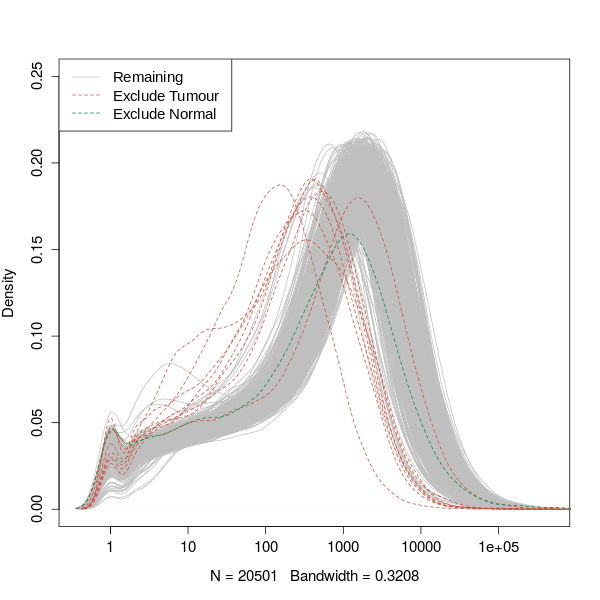
\includegraphics[width=0.4\textwidth]{fig2a.png}
        }%
        \subfigure[Voom normalised]{%
           \label{fig:density:second}
           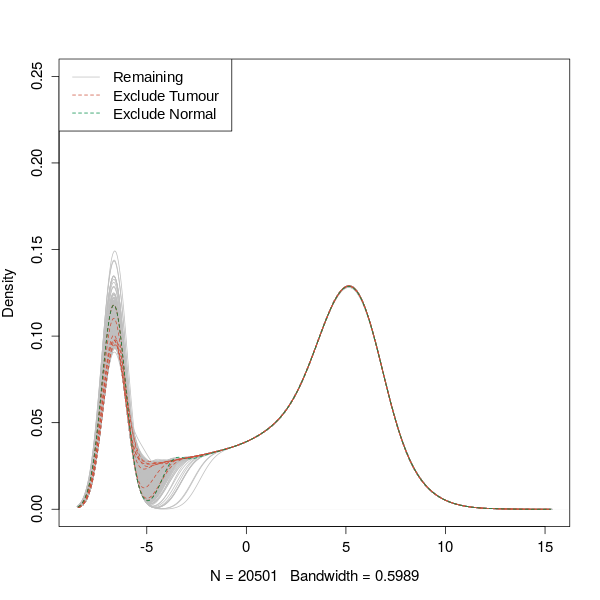
\includegraphics[width=0.4\textwidth]{fig2b.png}
        }%
%
\end{center}
\caption[Read count density]{\small \textbf{Read count density.} Sample density plots of raw counts on log-scale and voom normalised showing samples removed due to quality concerns.}
%}
\label{fig:density}
\end{mdframed}
\end{figure}

\begin{figure*}[!ht]
\begin{mdframed}
%  \resizebox{\textwidth}{!}{
         \begin{center}
%
        \subfigure[Mean raw counts (log-scale)]{%
            \label{fig:mean:first}
            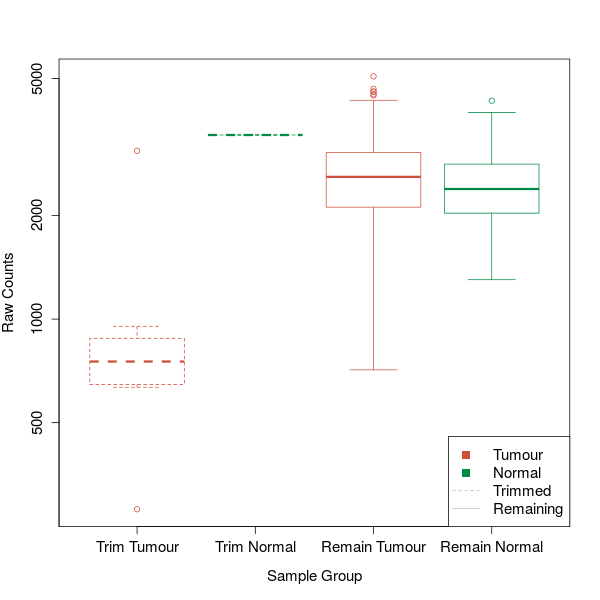
\includegraphics[width=0.4\textwidth]{fig3a.png}
        }%
        \subfigure[Mean voom normalised]{%
           \label{fig:mean:second}
           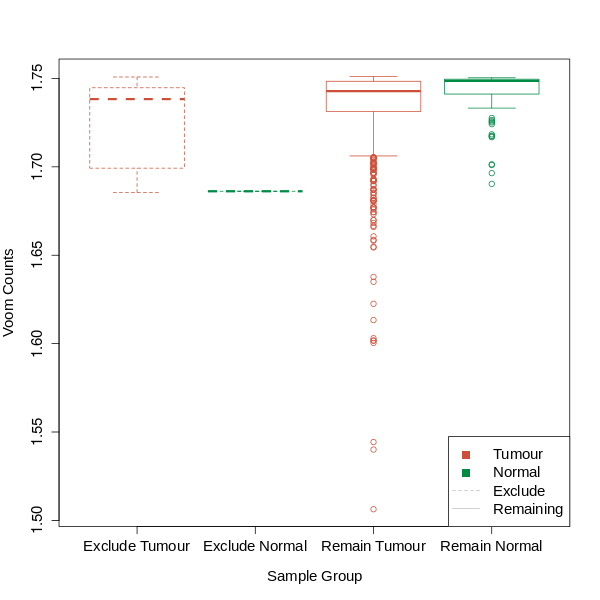
\includegraphics[width=0.4\textwidth]{fig3b.png}
        }%
%
    \end{center}
  \caption[Read count sample mean]{\small \textbf{Read count sample mean.} Boxplots of sample means for raw counts on log-scale and voom normalised show removed tumour samples with low mean read count.}
%}
\label{fig:boxplot}
\end{mdframed}
\end{figure*}


\subsection{Sample Triage} \label{methods:sample_qc}

The TCGA RNA-Seq data were assessed for batch effects using a correlation matrix of the log-transformed raw counts for which a heatmap (Euclidean distance, complete linkage) is shown in Figure \ref{fig:corr_map}. While no major batch effects were detectable between the samples, 9 samples were excluded due to poor correlation with the remaining samples, as detailed in Table \ref{tab:qc}. These samples showed unusual density plots compared to the rest of the dataset, and exhibited low mean read count in Figures \ref{fig:density} and \ref{fig:boxplot}. A heatmap showing key clinical properties of these excluded samples and their correlation with the remainder of the samples is shown in Figure \ref{fig:corr_map_part}, and a full correlation heatmap (Figure \ref{fig:corr_map}) shows these samples as relatively poorly correlated outliers in the bottom rows and left columns.
%In both of these cases, a shared tissue source site or patient donor indicates that variations in sample preparation are likely behind the outlying expression profiles. The Christiana Healthcare patients were sequenced in triplicate when replicate samples were rare in this dataset suggesting there were suspected errors in these samples during data generation which have lower mean read count than most of the dataset. %tangent
%Clinical characteristics over-represented in removed samples were ER+, ductal, state 2, luminal A or basal type tumours but these are the most common in the dataset. %relevance
After removal of these samples, the TCGA dataset used for analysis consisted of the remaining 1168 samples (from 1040 patients): 1049 tumour samples, 112 normal tissue for matched samples, and 7 metastases.

\begin{table*}[!ht]
\caption{Excluded Samples by Batch and Clinical Characteristics.}
\label{tab:qc}
\resizebox{\textwidth}{!}{
      \begin{tabular}{sc^c^c^c^c^c^c^c^c^c^c^c^c}
      \rowstyle{\bfseries}
        \multicolumn{1}{c}{\bfseries Tissue Source}		& \multicolumn{1}{sc}{\bfseries Type}   & \multicolumn{1}{sc}{\bfseries Batch} & \multicolumn{1}{sc}{\bfseries Plate} & \multicolumn{1}{sc}{\bfseries Patient} & \multicolumn{1}{sc}{\bfseries Samples} & \multicolumn{1}{c}{\bfseries p53}      & \multicolumn{1}{sc}{\bfseries Subtype}   & \multicolumn{2}{sc}{\bfseries Treatment (History)}	& \multicolumn{3}{sc}{\bfseries Clinical Subtypes (Stage)} \\
        \hline
       \rowcolor{black!10}
        A7 Christiana		& Tumour & 47	 & A227  & A0DB  &  1 of 3   & NA       & Luminal A & Mastectomy & (no)				& ER$+$  &  Ductal   	& (2)        \\
       \rowcolor{black!5}
        A7 Christiana		& Tumour & 96	 & A220  & A13D  &  1 of 3   & Wildtype & Luminal A & Mastectomy & (no)				& ER$+$  &  Ductal   	& (2)        \\
       \rowcolor{black!10}
        A7 Christiana		& Tumour & 96	 & A227  & A13E  &  1 of 3   & NA       & Basal     & Lumpectomy & (no) 				& ER$-$  &  Ductal   	& (2)        \\
       \rowcolor{black!5}
        A7 Christiana		& Tumour & 142	 & A277  & A26E  &  1 of 3   & NA       & Basal     & Lumpectomy & (no) 				& ER$+$  &  Ductal   	& (2)        \\
       \rowcolor{black!10}
        A7 Christiana		& Tumour & 47	 & A277  & A0DC  &  1 of 2   & NA       & Luminal A & Mastectomy & (yes)				& ER$+$  &  Lobular   	& (3)        \\
       \rowcolor{black!5}
        A7 Christiana		& Tumour & 142	 & A220  & A26I  &  1 of 2   & Mutant   & Basal     & Lumpectomy & (yes) 				& ER$-$  &  Ductal   	& (2)        \\
       \rowcolor{black!10}
        AC Intl Genomics	& Tumour & 177	 & A18M  & A2QH  &  2 of 2   & Mutant   & Basal     & Radical Mastectomy & (no) 			& ER$-$  &  Metaplastic   & (2)        \\
       \rowcolor{black!5}
        AC Intl Genomics	& Tumour & 177	 & A220  & A2QH  &  2 of 2   & Mutant   & Basal     & Radical Mastectomy & (no) 			& ER$-$  &  Metaplastic   & (2)        \\
       \rowcolor{black!10}
        GI ABS IUPUI		& Normal & 177	 & A16F  & A2C8  &  1 of 1   & NA       & Luminal A & Radical Mastectomy and Neoadjuvant & (no) 	& ER$+$  &  Ductal   	& (2)        \\
\hline
      \end{tabular}
}
\end{table*}


\subsection{Metagenes and the Singular Value Decomposition} \label{methods:metagene}
A ``metagene'' offers a consistent signal of pathway (expression) activation or inactivation by dimension reduction of a matrix, avoiding negatively correlated genes averaging out the signal of a mean-based centroid \citep{Huang2003}. Constructing these pathway metagenes used gene sets for Reactome and Gatza signatures (Gatza \textit{et al}., 2011; Gatza \textit{et al}., 2014) as specified above (see Section \ref{methods:gene_set}). The singular-value decomposition was performed ($X = U^{T} D V$ where $X$ is the data matrix of the gene set with genes $\times$ samples) and the leading eigenvector (first column of $V$) corresponding to the largest singular value was used as a metagene for the pathway gene set. To ensure consistent directionality of metagene signals, the median of the gene set in each sample was calculated and correlated against the metagene with the (arbitrary) metagene sign adjusted as needed to conform with the majority of the gene set (i.e., positive correlation between metagene and the median-based centroid). To ensure that genes and pathways were weighted equally, metagenes were derived from a z-transformed dataset of gene expression and samples were scaled (by fractional ranking) for each metagene so that they were comparable on a $[0,1]$ scale. 

\subsubsection{Candidate Triage and Integration with Screen Data} \label{methods:venn_analysis}
Candidate triage in combination with the experimental data was intended to integrate findings of the SLIPT analysis with an ongoing experiment project \citep{Chen2014, Telford2015}. The first procedure to compare the SLIPT gene candidates for \textit{CDH1} with an siRNA experimental screen \citep{Telford2015} was a direct comparison of the overlapping candidates, presented in a Venn diagram and tested with the $\chi^2$ test. Since these candidates modestly overlapped at the gene level (even when excluding genes not contained in both datasets), further gene set over-representation analysis was performed for pathways specific to each detection approach and the intersection of the two.

The pathway composition of the intersection was further verified by a permutation resampling analysis (as described in section \ref{methods:permutation}): the same number of genes detected by SLIPT were sampled randomly from the universe of genes tested by both approaches. These samplings were performed over 1 million iterations and the pathway over-representation was compared for each of the 1,652 reactome pathways.
%Adjusting for multiple comparisons was not needed here in a permutation analysis as the test $\chi^2$ statistics were directly used with the same degrees of freedom between expected and observed.
These over-representation scores ($\chi^2$) were compared the observed over-representation in the intersection of the SLIPT candidates, with the proportion of resamplings with higher $\chi^2$ values used for empirical p-values of pathway composition. Pathways for which no resamplings were occurred as high as the observed were reported as $p < 10^{-6}$. These empirical p-values were adjusted for multiple comparisons (FDR). Intersection size was not assumed to be constant across resamplings so similarly with the proportion of resamplings with higher or lower intersection size were used to evaluate significance of enrichment or depletion respectively (of siRNA candidate among SLIPT candidate genes).  

\section{Techniques}
Various statistical, computational, and bioinformatics techniques were performed throughout this thesis. This section describes these techniques and gives the parameters used unless otherwise specified. Where relevant, the R package implementation which provided the technique will be acknowledged. 

\subsection{Statistical Procedures and Tests}

As described in sections \ref{methods:heatmap} and \ref{methods:metagene}, the z-transform has been used to generate z-scores in various analyses in this thesis. Each row of dataset ($x$) is transformed into a scores ($z$) using the mean ($\mu$) and standard deviation ($\sigma$) of the data such that: $$ z = \frac{x - \mu(x)}{\sigma(x)} $$
This generates data where each row (gene) has a mean of 0 and standard deviation of 1. Where plotted as aa heatmap, any data more than 3 standard deviations above or below the mean is plotted as $3$ or $-3$ respectively.

Empirical Bayes differential expression analysis was performed using the \texttt{limma} R package \citep{limma}. Where specified, the Fisher's exact test, $\chi^2$ test, and correlation were used to measure associations between variables (as implemented in the \texttt{stats} R package \citep{R_core}). Unless otherwise specified, Pearson's correlation was used for correlation analyses ($r$) and coefficient of determination ($R^2$). Where these comparisons are discussed in more detail, Fisher's exact test and $\chi^2$ tests are supported by a table or Venn diagram, rendered with the \texttt{limma} R package \citep{limma}. In some analyses, correlation is furter supported by a scatter plot and a line of best fit dervied by least squares linear regression. 

The \texttt{t.test} function \citep{R_core} has also been used to implement the t-test to compare pairs of data. Where relevant, an analysis of variance (ANOVA) has been performed to report significance of multivariate predictors of outcomes, or least squares linear regression performed for the adjusted coefficient of determination ($R^2$) and F-statistic p-value to evaluate the fit of the predictor variables. For some analyses these are supported by boxplot or violinplot visualisation (rendered in R).

Multiple comparisons are adjusted by the Benjamini-Hochberg procedure to control the false discovery rate (FDR) unless otherwise specified \citep{fdr1995}. This procedure adjusts p-values to achieve an average of the proportion of false-positives among significant tests below a threshold, $\alpha$. The more stringent Holm-Bonferroni (Holm) procedure \citep{Holm1979} was also applied in some cases to adjust for multiple comparisons and control the family-wise error rate which adjusts p-values so that the probability that any one of the tests is a false-positive (type-1 error) below a threshold, $\alpha$.

\subsection{Gene Set Over-representation Analysis}
Gene set enrichment over-representation was performed to test whether there is an enrichment of a gene set (such as a biological pathway) among a group of input genes. Such input genes may be predicted synthetic lethal candidates or a subset defined by clustering (in section \ref{methods:clustering}) or comparison with experimental candidates (see section \ref{methods:venn_analysis}). Initially, these tests were performed using the GeneSetDB web tool \citep{genesetdb} hosted by the University of Auckland on the Reactome pathways \citep{Reactome}. Since the GeneSetDB tool used an older version of Reactome (version 40), it was difficult to directly compare with the results of other analysis (see sections \ref{methods:venn_analysis} and \ref{methods:permutation}) performed on version 52 (as described in  section \ref{methods:gene_set}). Thus an implementation of the hypergeometric test in R \citep{R_core} was used to test for over-representation against Reactome (version 52) pathways. Pathways containing less than 10 genes or more than 500 \citep[as performed in GeneSetDB by][]{genesetdb} were excluded before adjusting for multiple comparisons.

\subsection{Clustering} \label{methods:clustering}
Clustering analysis when performed uses unsupervised hierarchical clustering with complete linkage (distance calculated from the furthest possible pairing). For correlation matrices or multivariate normal parameters (e.g., $\Sigma$), the distance metric used was Euclidean distance. For empirical or simulated gene and pathway expression data correlation distance was used, calculated by $distance = 1 - cor(t(x))$ where $cor$ is Pearson's correlation and $t(x)$ is the transpose of the expression matrix. 

\subsection{Heatmap} \label{methods:heatmap}
Standardised z-scores of the data were used to plot heatmaps on an appropriate scale. Raw (log-scale) read counts or voom normalised counts per gene (as specified) were plotted  as normalised z-scores on a $[-3,+3]$ blue-red scale. Similarly, correlations were plotted on a $[-1,+1]$ blue-red scale. These heatmaps were performed using the linkage and distance specified for the clustering performed in Section \ref{methods:clustering}. The \texttt{gplots} R package \citep{gplots} was used to generate many of the heatmaps throughout this thesis, along with a customised heatmap function (released as \texttt{heatmap.2x}). Where clearly specified, data have been split into subsets with clustering performed separately on each subset with these plotted alongside each other.

\subsection{Modeling and Simulations} \label{methods:simulation}
Statistical modeling and simulations have been used to test various synthetic lethal detection procedures on simulated data. This involves constructing a statistical model of how synthetic lethality would appear in (continuous normally distributed) gene expression data. Where presented (in section \ref{methods:SL_Model}), the assumptions of the model are stated clearly. The model allows sampling from a multivariate normal distribution (using the \texttt{mvtnorm} R package \citep{Genz2009, mvtnorm}) to generate simulated data with known underlying synthetic lethal partners (detailed in section \ref{methods:simulating_SL}). We can test whether statistical procedures, including those developed in this thesis (presented in section \ref{methods:SLIPT}), are capable of detecting them upon this simulated data. This multivariate normal simulation procedure also enables the inclusion of correlation structure which is either given as correlated blocks of genes or derived from pathway structures (as detailed in section \ref{methods:graphsim}).

If this multivariate normal distribution was sampled once and the procedure to add known synthetic lethal partners was performed, it generates a simulated dataset. Performing this simulation procedure and testing with a synthetic lethal detection procedure iteratively, these simulations can be used to assess the statistical performance of the detection procedure. The number of iterations (\texttt{Reps}) will be given for each simulation result. Typically, these are performed 1000 or 10,000 times depending on computational feasibility of doing so on larger datasets. 

Several measures of statistical performance were used to assess the simulations. The following measures used the final classification of the detection procedure, statistical significance for $\chi^2$, significance and directional criteria met for SLIPT (see section \ref{methods:SLIPT}), and an arbitrary threshold: $<-0.2$ and $>+0.2$ for  negative correlation and correlation respectively. Sensitivity (or ``true positive rate'') was measured as the proportion of known synthetic lethal partners predicted to be synthetic lethal. Specificity (or ``true negative rate'') was measured as the proportion of known non-synthetic lethal partners predicted not to be synthetic lethal. The ``false discovery rate'' (also used in adjusting for multiple comparisons) was measured here as the proportion of known non-synthetic lethal partners out of all putative partners predicted by the detection procedure. Statistical ``accuracy'' is the proportion of true predictions for a detection procedure, which is both the correctly predicted known synthetic lethal partners and correctly negative known non-synthetic lethal partners.

\subsubsection{Receiver Operating Characteristic (Performance)}
A more general procedure to measure the statistical performance of a simulation is the Receiver Operating Characteristic (ROC) curve which does not assume a threshold for classification of synthetic lethality but demonstrates the trade-off of sensitivity and specificity \citep{Zweig1993, Fawcett2006, Akobeng2007}. These curves (implemented with the \texttt{ROCR} R package \citep{ROCR}) plot the True Positive Rate (sensitivity) against the False Positive Rate ($1-$specificity) as the prediction threshold is varied. An ideal detection method will have a true positive rate of 1 and a false positive rate of 0, hence the Area Under the ROC curve (AUC or AUROC) is a measure of statistical performance for a detection procedure accounting for this trade-off. AUROC values are typically range from 0.5 the value expected by random chance to 1 for an optimal detection method, however it is possible for an AUROC below 0.5 for a poor detection method that performs worse than random chance. An cancer biology, an AUROC of approximately $0.8$ is a predictive biomarker suitable for publication \citep{Hajian-Tilaki2013} but predictors with lower AUROC values may still be informative depending on the context. In this thesis, the AUROC values varies widely across simulation parameters and a primarily used for comparisons across these parameters, although they can also be used to refine thresholds for optimal classification. 

\subsection{Resampling Analysis} \label{methods:permutation}
Resampling analyses (e.g., ``permutation'' analysis) are used to statistically test the significance of an observation without assuming the underlying distribution of expected test statistics \citet{Collingridge2013}. Instead these are derived from randomly shuffling test statistics or randomly sampling predicted candidates. For the purposes of this thesis, this involved randomly sampling genes from those tested to be analysed as putative synthetic lethal candidates. This was performed both for testing the significance of pathway composition in the intersection with experimental gene candidates (section \ref{methods:venn_analysis}) and for assessing the significance of pathway structure among synthetic lethal candidates (section \ref{methods:network_permutation}).

These were analysed to compare the observed synthetic lethal genes against values derived from randomly sampling the same number of genes as observed by synthetic lethal from among the genes tested. Sampling iteratively across many resampling procedures, these resampling-based values form a null distribution that would be observed if the null hypothesis were true. Thus the proportion of resampling-based values across these iterations that are greater than or equal to that observed, forms an empirically derived p-value to test significance.

Resampling was performed for comparison (in section \ref{methods:venn_analysis}) with fixed experimental screen candidates \citep{Telford2015} both resampling the number of genes overlapping with the screen candidates and test statistics for pathway enrichment. Resampling analysis was also applied to shortest paths and network metrics (in section \ref{methods:network_permutation}) to test significance of directional relationships between synthetic lethal candidate genes within pathway structures.

The number of iterations determines the accuracy of these p-values. For pathway composition (in section \ref{methods:venn_analysis}), a million iterations were performed using high performance computing (as detailed in section \ref{methods:HPC}) to provide sufficient accuracy after adjusting for multiple comparisons across pathways. For the purposes of network analysis (in section \ref{methods:network_permutation}), a thousand iterations were sufficient to reject the null hypothesis for the majority of pathways tested before adjusting for multiple comparisons, and thus further iterations were not performed.

\section{Pathway Structure Methods}

\subsection{Network and Graph Analysis}

Networks are important in considering the structure of relationships in molecular biology, including gene regulation, kinase cellular signaling, and metabolic pathways \citep{Barabasi2004}. Network theory is an interdisciplinary field which combines the approaches of computer science with the metrics and fundamental principles of graph theory, an area of pure mathematics dealing with relationships between sets of discrete elements. The vast amounts of molecular and cellular data from high-throughput technologies have enabled the application of network-based and genome-wide bioinformatics analysis to examine the complexity of a cell at the molecular level and understand aberrations in cancer. This thesis uses various metrics and analysis procedures developed in Graph and Network theory to analyse graph structure of biological pathways. Where feasible, these have been implemented using the \texttt{igraph} R package with such procedures described below \citep{igraph}. Custom R functions to perform more complex analysis and visualisation of iGraph data objects will be described later.

Graph theory is a branch of pure mathematics which deals with the properties of sets of discrete objects (referred to as a `node' or `vertex`) with some pairs are joined (by a `link' or an `edge`). While a seemingly reductionist abstraction to mathematically study relationships, graph theory serves has applications in a wide range of studies including life sciences. Network theory is the sub-discipline of graph theory which deals with networks which has become popular due to the vast potential for applications of networks \citep{vanSteen2010}. 

Applications vary depending on the situation modelled, particularly in how the edges between vertices are defined, whether they are directed or weighted, and whether multiple redundant edges between a pair of vertices (referred to as `parallel edges`) or edges connecting a vertex to itself (referred to as `loops`) are permitted in the model. Networks are defined such that the edges represent a relationship between the vertices and may be directed, weighted, or contain parallel edges or loops depending on the application \citep{vanSteen2010}. Unless otherwise stated, graph structures and networks in thesis will be unweighted and have no parallel edges or loops. Where a directional relationship is known or modelled, it will be represented with a directed edge in a directed graph.

\subsection{Sourcing Graph Structure Data} \label{methods:graph_data}
Pathway Commons interaction data was sourced using the paxtools-4.3.0 Java application on October 6th 2015 \citep{PathwayCommons, paxtools}. This utility was used to source `sif' format interaction data into R \citep{R_core}, from which the human Reactome (version 52) dataset of interactions was imported \citep{Reactome}, matching those used for pathway enrichment analysis. These interactions were used to construct an adjacency matrix for the Reactome network and subnetworks corresponding to each relevant biological pathway. 

\subsection{Constructing Pathway Subgraphs} \label{methods:subgraphs}
Subgraphs for each relevant pathway were constructed by matching the nodes in the complete Reactome network to the pathway gene sets (as derived in section \ref{methods:gene_set}). A subgraph with adjacent nodes was constructed by adding nodes which have an edge with a gene in the pathway gene set. The pathways these adjacent nodes belong to were added to form a ``meta-pathway'' to account for the possibility for nodes within the pathway being linked by the surrounding graph structure.

\subsection{Network Analysis Metrics} \label{methods:network_metrics}
The existing network analysis measures applied in this thesis (as described below) used an implementation in the \texttt{igraph} R package where it was available \citep{igraph}. Otherwise, custom features were developed for analysis of iGraph objects in R and released as \texttt{igraph.extensions} (as described in section \ref{methods:igraph_extensions}).

Vertex degree is the number of edges a node has and is a fundamental measure of the importance and connectivity of a network \citep{vanSteen2010}. More connected nodes, such as network hubs, will have a higher vertex degree relative to other nodes. For the purposes of this thesis, vertex degree ignored edge direction with loops (edges with itself) and double edges to the same node excluded.

A fundamental concept in network analysis is a ``shortest path'', that is the shortest route via edges between any two particular nodes in a network. These are computed by Dijstra's algorithm \citep{Dijkstra1959} in the \texttt{igraph} R package \citep{igraph}. Where applicable paths will only use directed edges in a particular direction. Shortests paths are a useful measure of how close nodes are in a network. This is used to compute information centrality, and for further analysis of pathway structure (as described in section \ref{methods:pathway_str}).

Network centrality is an alternative measure of the importance or influence of a node to the graph structure \citep{Borgatti2005}. Various strategies are used to derive centrality,  typically based on how connected the node is or the impact of node removal on the connectivity of the network. One of the most notable is the ``PageRank'' algorithm, a refinement of eigenvector centrality based on the eigenvectors of the adjacency matrix \citep{Brin1998}. This is implemented in the \texttt{igraph} R package \citep{igraph}.

Another network centrality measure that has been previously applied to biological protein interaction networks \citep{Kranthi2013} is the ``information centrality''. The information centrality of a node is the relative impact on efficiency (transmission of information via shortest paths) of the network when the node is removed. That is the centrality ($C$) \citep{Kranthi2013} for node $n$ in graph $G$ is defined as: $$C_n = \frac{E(G)-E(G')}{E(G)}$$ where $G'$ is the subgraph with the node removed and $E$ is the efficiency \citep{Latora2001} derived from shortest paths ($d_{ij}$ between nodes $i$ and $j$) as: $$E(G) = \frac{2}{N(N-1} \sum_{i<j \in G}^{} \frac{1}{d_{ij}}$$ The efficiency of the network can be derived from shortest paths implemented in the \texttt{igraph} R package and the iterative network centrality computation of each node has been released as an R package (\texttt{info.centrality}) and included in the \texttt{igraph.extensions} package.

\section{Implementation}
%\subsection{Computational Tools and Enabling Biological Research (remove/state assumptions only)}
%\subsubsection{Computational Tools for Biological Research}
%In addition to hosting data repositories on the web, tools developed with computational expertise have had wider benefit in  genetics research. One of the main impacts of a techniques developed from computer science is the alignment of reads, to either assemble a genome \textit{de novo} from it's reads or map reads to a pre-existing reference genome. Mapping reads is commonplace to call variants between samples, this is useful for studies of human disease interested in risks of these variants or wider application such as comparing populations or species in an evolution phylogeny. Mapping reads has further utility in functional genetics to identify which regions or a genome are expressed or have DNA methylation. Similarly, mapping is used to map RNA-Seq or Bisulfite-Seq reads to measure gene expression or DNA methylation across the genome in a cohort or sample. While mapping is not performed in this thesis, it has performed an important role in the adoption of genomics in genetics research.



\subsection{Computational Resources and Linux Utilities}

Several computers were used to process and store data during this thesis (as summarised in Table \ref{tab:computers}), running different versions of Linux operating systems, including a personal laptop computer, laboratory desktop machine, departmental server, and the New Zealand eScience Infrastructure Intel Pan high-performance computing cluster (a supercomputer based at the University of Auckland). Each of these systems support a 64-bit architecture. Current workflows on local machines use Elementary OS (based on the Ubuntu versions given in Table \ref{tab:computers}) and interacting with these via ZSH shell. However, Ubuntu OS and the Bourne Again SHell (bash) were used at the inception of this project and bash is continues to be used for running scripts. Various Linux applications and command-line utilities were used on these machines (as summarised in Table \ref{tab:computers_linux}). As such, the workflows developed in this project should be backwards-compatible with Ubuntu Linux (and other derivatives). The majority of novel methodology and implementations were performed in R which is a cross-platform language, packages developed in R will be available for users of Linux, Mac, and Windows machines.  


\begin{table}[!ht]
\centering
\caption{Computers used during Thesis}
\label{tab:computers}
\makebox[\textwidth][c]{
\resizebox{\textwidth}{!}{
\begin{tabular}{r|l|l|l|l|}
%\cline{2-5}
\multicolumn{1}{r}{}                        & \multicolumn{1}{l}{\bfseries Viao Laptop}                                     & \multicolumn{1}{l}{\bfseries Lab Machine}                                   & \multicolumn{1}{l}{\bfseries Biochem Server}                                     & \multicolumn{1}{l}{\bfseries NeSI Pan Cluster}                               \\
\cline{2-5}
\rowcolor{gray!25}
\multicolumn{1}{r|}{\cellcolor{white}Operating System (OS)}  & \begin{tabular}[c]{@{}l@{}}Elementary OS\\ Freya 0.3.2\end{tabular} & \begin{tabular}[c]{@{}l@{}}Elementary OS\\ Loki 0.4\end{tabular}  & \begin{tabular}[c]{@{}l@{}}Red Hat Enterprise\\ Maipo 7.2\end{tabular} & \begin{tabular}[c]{@{}l@{}}Cent OS\\ Final 6.4\end{tabular} \\  \cline{2-5}
\multicolumn{1}{r|}{\cellcolor{white}Upstream OS}            & \begin{tabular}[c]{@{}l@{}}Ubuntu LTS\\ Trusty 14.04\end{tabular}   & \begin{tabular}[c]{@{}l@{}}Ubuntu LTS\\ Xenial 16.04\end{tabular} &                                                                        &                                                             \\  \cline{2-5}

\rowcolor{gray!25}
\multicolumn{1}{r|}{\cellcolor{white}Linux Kernel}           & 3.19.0-65-generic                                                   & 4.4.0-36-generic                                                  & 3.10.0-327.36.2.el7.x86\_64                                            & 2.6.32-504.16.2.el6.x86\_64                    \\
\cline{2-5}
\multicolumn{1}{r|}{\cellcolor{white}Shell: bash}            & 4.3.11(1)                                                           & 4.3.46(1)                                                         & 4.2.46(1)                                                              & 4.2.1(1)                                       \\
\cline{2-5}

\rowcolor{gray!25}
\multicolumn{1}{r|}{\cellcolor{white}Shell: zsh}             & 5.0.2                                                               & 5.1.1                                                             & 5.0.2                                                                  & 5.2                                            \\
\cline{2-5}
\end{tabular}
}}
\end{table}


\begin{table}[!ht]
\centering
\caption{Linux Utilities and Applications used during Thesis}
\label{tab:computers_linux}

\resizebox{\textwidth}{!}{
\begin{tabular}{ll|l|l|l|l|}
%\cline{3-6}
\cellcolor{white}                                                      & \multicolumn{1}{l}{}                         & \multicolumn{1}{l}{\bfseries Viao Laptop}                           & \multicolumn{1}{l}{\bfseries Lab Machine}                         & \multicolumn{1}{l}{\bfseries Biochem Server}                           & \multicolumn{1}{l}{\bfseries NeSI Pan Cluster}                               \\
\cline{2-6}
\rowcolor{gray!25}
\cellcolor{white}                                                      & \multicolumn{1}{|l|}{OS}                     & \begin{tabular}[c]{@{}l@{}}Elementary OS\\ Freya 0.3.2\end{tabular} & \begin{tabular}[c]{@{}l@{}}Elementary OS\\ Loki 0.4\end{tabular}  & \begin{tabular}[c]{@{}l@{}}Red Hat Enterprise\\ Maipo 7.2\end{tabular} & \begin{tabular}[c]{@{}l@{}}Cent OS\\ Final 6.4\end{tabular} \\
\cline{2-6}
\cellcolor{white}                                                      & \multicolumn{1}{|l|}{Linux Kernel}           & 3.19.0-65-generic                                                   & 4.4.0-36-generic                                                  & 3.10.0-327.36.2.el7.x86\_64                                            & 2.6.32-504.16.2.el6.x86\_64                    \\
\hline

\rowcolor{gray!25}
\cellcolor{white} Scripting                                            & \multicolumn{1}{|l|}{Shell\: bash}            & 4.3.11(1)                                                           & 4.3.46(1)                                                         & 4.2.46(1)                                                              & 4.2.1(1)                                       \\
\cline{2-6}
\cellcolor{white}                                                      & \multicolumn{1}{|l|}{Shell\: zsh}             & 5.0.2                                                               & 5.1.1                                                             & 5.0.2                                                                  & 5.2                                            \\
\hline

\rowcolor{gray!25}
\cellcolor{white} Programming                                          & \multicolumn{1}{|l|}{Python}                 & 2.7.6                                                               & 2.7.12                                                            & 2.7.5                                                                  &                                                \\
\cline{2-6}
\cellcolor{white}                                                      & \multicolumn{1}{|l|}{Java}                   & 1.8.0\_101                                                          & 9-ea                                                              & 1.8.0\_101                                                             &                                                \\
\cline{2-6}

\rowcolor{gray!25}
\cellcolor{white}                                                      & \multicolumn{1}{|l|}{C$++$}                  & 4.8.4                                                               & 5.4.0                                                             & 4.8.5                                                                  & 4.4.7                                          \\
\hline
\cellcolor{white} Text Editor                                          & \multicolumn{1}{|l|}{nano}                   & 2.2.6                                                               & 2.5.3                                                             & 2.3.1                                                                  & 2.0.9                                          \\
\cline{2-6}

\rowcolor{gray!25}
\cellcolor{white}                                                      & \multicolumn{1}{|l|}{kile (\LaTeX)}          & 2.1.3                                                               & 2.1.3                                                             &                                                                        &                                                \\
\hline
\cellcolor{white} Version Control                                      & \multicolumn{1}{|l|}{git}                    & 1.9.1                                                               & 2.11.0                                                            & 1.7.1                                                                  & 1.8.3.1                                        \\
\hline

\rowcolor{gray!25}
\cellcolor{white} Shell Utilities                                      & \multicolumn{1}{|l|}{sed}                    & 4.4.2                                                               & 4.4.2                                                             & 4.4.2                                                                  & 4.4.1                                          \\
\cline{2-6}
\cellcolor{white}                                                      & \multicolumn{1}{|l|}{grep}                   & 2.16-1                                                              & 2.25-1                                                            & 2.20                                                                   & 2.6.3                                          \\
\cline{2-6}

\rowcolor{gray!25}
\cellcolor{white}                                                      & \multicolumn{1}{|l|}{nohup}                  & 8.21                                                                & 8.25                                                              & 8.22                                                                   & 8.4                                            \\
\hline
\cellcolor{white} Typesetting                                          & \multicolumn{1}{|l|}{\TeX}                   & 3.1415926                                                           & 3.14159265                                                        &                                                                        &                                                \\
\cline{2-6}

\rowcolor{gray!25}
\cellcolor{white}                                                      & \multicolumn{1}{|l|}{TexLive (\LaTeX)}       & 2013                                                                & 2015                                                              &                                                                        &                                                \\
\cline{2-6}
\cellcolor{white}                                                      & \multicolumn{1}{|l|}{PDF\TeX}                & 2.5-1                                                               & 2.6                                                               &                                                                        &                                                \\
\cline{2-6}

\rowcolor{gray!25}
\cellcolor{white}                                                      & \multicolumn{1}{|l|}{pandoc}                 & 1.12.2.1                                                            & 1.16.0.2                                                          &                                                                        &                                                \\
\hline
\cellcolor{white} Remote Computing                                     & \multicolumn{1}{|l|}{slurm scheduler}        &                                                                     &                                                                   &                                                                        & 16.05.6                                        \\
\cline{2-6}

\rowcolor{gray!25}
\cellcolor{white}                                                      & \multicolumn{1}{|l|}{OpenSSH}                & 7.2p2                                                               & 7.2p2                                                             & 6.6.1                                                                  & 5.3p1                                          \\
\cline{2-6}
\cellcolor{white}                                                      & \multicolumn{1}{|l|}{OpenSSL}                & 1.0.2g                                                              & 1.0.2g                                                            & 1.0.01e-fips                                                           & 1.0.01e-fips                                   \\
\cline{2-6}

\rowcolor{gray!25}
\cellcolor{white}                                                      & \multicolumn{1}{|l|}{rsync}                  & 3.1.0p31                                                            & 3.1.1p31                                                          & 3.0.9p30                                                               &                                                \\
\cline{2-6}
\cellcolor{white}                                                      & \multicolumn{1}{|l|}{Globus Online Transfer} &                                                                     &                                                                   & 3.1                                                                    & 3.1                                            \\
\cline{2-6}

\rowcolor{gray!25}
\cellcolor{white}                                                      & \multicolumn{1}{|l|}{Cisco AnyConnect VPN}   &                                                                     & 3.1.05170                                                         &                                                                        &                                                \\
\hline
\cellcolor{white} Image Processing                                     & \multicolumn{1}{|l|}{Inkscape}               & 0.48.4                                                              & 0.91                                                              &                                                                        &                                                \\
\cline{2-6}

\rowcolor{gray!25}
\cellcolor{white}                                                      & \multicolumn{1}{|l|}{GIMP}                   & 2.8.10                                                              & 2.8.16                                                            &                                                                        &                                                \\
\cline{2-6}
\cellcolor{white}                                                      & \multicolumn{1}{|l|}{ImageMagick}            & 6.7.7.10-6                                                          &                                                                   &                                                                        &                                                \\
\hline                                
\end{tabular}
}
\end{table}

\begin{table}[!ht]
\centering
\caption{R Installations used during Thesis}
\label{tab:computers_r}
\resizebox{\textwidth}{!}{
\begin{tabular}{ll|l|l|l|l|}
%\cline{3-6}
                                        & \multicolumn{1}{l}{}              & \multicolumn{1}{l}{\bfseries Viao Laptop}                           & \multicolumn{1}{l}{\bfseries Lab Machine}                         & \multicolumn{1}{l}{\bfseries Biochem Server}                           & \multicolumn{1}{l}{\bfseries NeSI Pan Cluster}           \\
\cline{2-6}
\rowcolor{gray!25}
\cellcolor{white}                       & \multicolumn{1}{|l|}{OS}          & \begin{tabular}[c]{@{}l@{}}Elementary OS\\ Freya 0.3.2\end{tabular} & \begin{tabular}[c]{@{}l@{}}Elementary OS\\ Loki 0.4\end{tabular}  & \begin{tabular}[c]{@{}l@{}}Red Hat Enterprise\\ Maipo 7.2\end{tabular} & \begin{tabular}[c]{@{}l@{}}Cent OS\\ Final 6.4\end{tabular} \\
\hline
\cellcolor{white} Programming           & \multicolumn{1}{|l|}{R}           & 3.3.2                                                               & 3.3.2                                                             & 3.3.1                                                                  & 3.3.0-intel (module)                          \\
\hline

\rowcolor{gray!25}
\cellcolor{white} Development           & \multicolumn{1}{|l|}{RStudio}     & 1.0.136                                                             & 1.0.136                                                           & 1.0.136 (server)                                                       &                                                \\
\hline
\end{tabular}
}
\end{table}

\subsection{R Language and Packages}


The R programming language has been used for the majority of this thesis. Current R installations across the machines used are given in Table \ref{tab:computers_r}. Local machines currently run the latest version of the R (at the time of writing) and remote machines run the versions and modules as managed by the system administrator. Various scripts and packages in this thesis were developed or run in previous versions of RStudio and R but these run without error in the current version of R (and the older versions on remote machines). The R packages developed during this thesis are given in Table \ref{tab:computers_r_packages_dev} with the relevant sections describing their implementation and use where appropriate, in addition to further details on these functions in section \ref{methods:r_packages}. Various R packages were used throughout this thesis (as detailed in Table \ref{tab:computers_r_packages} with versions specified), which were not updated when they would change the functionality of scripts or functions in packages, in particular imported data from annotation packages (used to define gene sets) have been saved as local files to continue using stable versions of these pathway data (across machines). This is a summary of the key packages which (in addition to their dependencies) have been used throughout this project. Where a package implementation has been central to the methods applied, they are described in more detail in the relevant section. A full table of packages used in this thesis can be found in the Appendix (Table \ref{tab:computers_r_packages_full}).  

\begin{table}[!ht]
\centering
\caption{R Packages Developed during Thesis}
\label{tab:computers_r_packages_dev}
\resizebox{\textwidth}{!}{
\begin{tabular}{l|l|l|c|}
%\cline{2-4}
\multicolumn{1}{l}{}           & \multicolumn{1}{l}{\bfseries Package Name} & \multicolumn{1}{l}{\bfseries Description                                                   and GitHub Repository}                                                                   & \multicolumn{1}{c}{\bfseries Section} \\
\cline{2-4}  \rowcolor{gray!25} \cellcolor{white}
                               & \multicolumn{1}{l|}{\texttt{slipt}}        & \begin{tabular}[c]{@{}l@{}}Synthetic lethal detection by SLIPT (to accompany publication)  \\ \url{https://github.com/TomKellyGenetics/slipt}                         \end{tabular} & \ref{methods:SLIPT}  \\
\hline
visualisation                  & \texttt{vioplotx}                          & \begin{tabular}[c]{@{}l@{}}Customised violin plots (based on \texttt{vioplot})             \\ \url{https://github.com/TomKellyGenetics/vioplotx}                      \end{tabular} &                              \\
\cline{2-4}

\rowcolor{gray!25} \cellcolor{white}
                               & \texttt{heatmap.2x}                      & \begin{tabular}[c]{@{}l@{}}Customised heatmaps (based on \texttt{gplots})                  \\ \url{https://github.com/TomKellyGenetics/heatmap.2x}                    \end{tabular} & \ref{methods:heatmap} \\
\hline
\texttt{igraph.extensions}     & \texttt{igraph.extensions}               & \begin{tabular}[c]{@{}l@{}}Meta-package to install the follow iGraph functions             \\ \url{https://github.com/TomKellyGenetics/igraph.extensions}             \end{tabular} & \ref{methods:igraph_extensions}    \\
\cline{2-4}

\rowcolor{gray!25} \cellcolor{white}
                               & \texttt{plot.igraph}                     & \begin{tabular}[c]{@{}l@{}}Custom plotting of directed graphs                              \\ \url{https://github.com/TomKellyGenetics/plot.igraph}                   \end{tabular} & \ref{methods:network_metrics}      \\
\cline{2-4}
                               & \texttt{info.centrality}                 & \begin{tabular}[c]{@{}l@{}}Computing information centrality from network efficiency        \\ \url{https://github.com/TomKellyGenetics/info.centrality}               \end{tabular} & \ref{methods:graphsim}\\
\cline{2-4}

\rowcolor{gray!25} \cellcolor{white}
                               & \texttt{pathway.structure.permutation}   & \begin{tabular}[c]{@{}l@{}}Testing pathway structure with resampling analysis              \\ \url{https://github.com/TomKellyGenetics/pathway.structure.permutation} \end{tabular} & \ref{methods:network_permutation}  \\
\cline{2-4}
                               & \texttt{graphsim}                        & \begin{tabular}[c]{@{}l@{}}Generating simulated expression from graph structures           \\ \url{https://github.com/TomKellyGenetics/graphsim}                      \end{tabular} & \ref{methods:graphsim}\\
\hline 
\end{tabular} 
}
\end{table}


%\resizebox{\textwidth}{!}{
\setlength{\LTleft}{-20cm plus -1fill}
\setlength{\LTright}{\LTleft}

\begin{longtable}{|llll|}
\caption{R Packages used during Thesis}
\label{tab:computers_r_packages}
%\\ hline
\\
\multicolumn{1}{l}{\bfseries Package}      & \multicolumn{1}{l}{\bfseries Version Used} & \multicolumn{1}{l}{\bfseries Built} & \multicolumn{1}{l}{\bfseries Repository}      \\
\hline  \rowcolor{gray!25}
colorspace   & 1.3-2          & 3.3.1 & CRAN            \\
\hline
curl         & 2.3            & 3.3.1 & CRAN            \\
\hline  \rowcolor{gray!25}
data.table   & 1.9.6          & 3.3.1 & CRAN            \\
\hline
dendextend   & 1.4.0          & 3.3.2 & CRAN            \\
\hline  \rowcolor{gray!25}
DBI          & 0.5-1          & 3.3.1 & CRAN            \\
\hline
devtools     & 1.12.0         & 3.3.1 & CRAN            \\
\hline  \rowcolor{gray!25}
dplyr        & 0.5.0          & 3.3.1 & CRAN            \\
\hline
ggplot2      & 2.2.1          & 3.3.1 & CRAN            \\
\hline  \rowcolor{gray!25}
git2r        & 0.18.0         & 3.3.1 & CRAN            \\
\hline
gplots       & 3.0.1          & 3.3.1 & CRAN            \\
\hline  \rowcolor{gray!25}
gtools       & 3.5.0          & 3.3.1 & CRAN            \\
\hline
igraph       & 1.0.1          & 3.3.1 & CRAN            \\
\hline  \rowcolor{gray!25}
matrixcalc   & 1.0-3          & 3.3.1 & CRAN            \\
\hline
mclust       & 5.2.2          & 3.3.1 & CRAN            \\
\hline  \rowcolor{gray!25}
mvtnorm      & 1.0-6          & 3.3.1 & CRAN            \\
\hline
org.Hs.eg.db & 3.1.2          & 3.1.2 & Bioconductor    \\
\hline  \rowcolor{gray!25}
openssl      & 0.9.6          & 3.3.1 & CRAN            \\
\hline
plyr         & 1.8.4          & 3.3.1 & CRAN            \\
\hline  \rowcolor{gray!25}
purrr        & 0.2.2          & 3.3.1 & CRAN            \\
\hline
reactome.db  & 1.52.1         & 3.2.1 & Bioconductor    \\
\hline  \rowcolor{gray!25}
RColorBrewer & 1.1-2          & 3.3.1 & CRAN            \\
\hline
Rcpp         & 0.12.9         & 3.3.1 & CRAN            \\
\hline  \rowcolor{gray!25}
ROCR         & 1.0-7          & 3.3.1 & CRAN            \\
\hline
roxygen2     & 6.0.1          & 3.3.2 & CRAN            \\
\hline  \rowcolor{gray!25}
shiny        & 1.0.0          & 3.3.1 & CRAN            \\
\hline
snow         & 0.4-2          & 3.3.1 & CRAN            \\
\hline  \rowcolor{gray!25}
testthat     & 1.0.2          & 3.3.2 & CRAN            \\
\hline
tidyr        & 0.6.1          & 3.3.2 & CRAN            \\
\hline  \rowcolor{gray!25}
tidyverse    & 1.1.1          & 3.3.2 & GitHub (hadley) \\
\hline
sm           & 2.2-5.4        & 3.3.1 & CRAN            \\
\hline  \rowcolor{gray!25}
Unicode      & 9.0.0-1        & 3.3.2 & CRAN            \\
\hline
vioplot      & 0.2            & 3.3.1 & CRAN            \\
\hline  \rowcolor{gray!25}
viridis      & 0.3.4          & 3.3.2 & CRAN            \\
\hline
xml2         & 1.1.1          & 3.3.2 & CRAN            \\
\hline  \rowcolor{gray!25}
xtable       & 1.8-2          & 3.3.1 & CRAN            \\
\hline
zoo          & 1.7-14         & 3.3.1 & CRAN            \\
\hline  \rowcolor{gray!25}
graphics     & 3.3.2          & 3.3.2 & base            \\
\hline
grDevices    & 3.3.2          & 3.3.2 & base            \\
\hline  \rowcolor{gray!25}
cluster      & 2.0.5          & 3.3.1 & base            \\
\hline
graphics     & 3.3.2          & 3.3.2 & base            \\
\hline  \rowcolor{gray!25}
grDevices    & 3.3.2          & 3.3.2 & base            \\
\hline
Matrix       & 1.2-8          & 3.3.1 & base            \\
\hline  \rowcolor{gray!25}
stats        & 3.3.2          & 3.3.2 & base            \\
\hline
\end{longtable}


\subsection{High Performance and Parallel Computing} \label{methods:HPC}
Another enabling technology for bioinformatics is parallel computing, performing independent operations in separate cores: this ``multithreading'' is widely used to increase the time to compute results. Bioinformatics is particularly amenable to this since performing multiple iterations of a simulation or testing separate genes is often ``embarrassingly parallel``, being completely independent of the results of each other. As such parallel computing is offered by many high-performance ``supercomputers'' including national research infrastructure.

The New Zealand eScience Infrastructure (NeSI) is a computating resource providing the Intel Pan cluster hosted by the University of Auckland \citep{NeSI}. The Pan cluster used throughout this thesis project to optimise and perform computations which would have otherwise been infeasible in the timeframe of thesis. Such technological developments and infrastructure initiatives have enabled bioinformatics research including this project.  High performance computing on the Pan cluster was used extensively in this project including for resampling analysis (in sections \ref{methods:permutation} and \ref{methods:network_permutation}), calculating information centrality (in section \ref{methods:network_metrics}), and in simulations (in sections \ref{methods:simulation}, \ref{methods:simulation_SL_expression}, and \ref{methods:graphsim})

Scripts and data were transferred between the Pan cluster and University of Otago computing resources by \texttt{rsync} or the Globus file transfer service \citep{Globus}. R scripts \citep{R_core} were run in parallel with the ``simple network of workstations'' \texttt{snow} R package \citet{snow}. This utilised the ``message passing interface'' \citep{Rmpi} when it was feasible with memory requirements to run in parallel across multiple compute nodes, otherwise SOCKS was used to access multiple cores within an instance of R and pass input data to them. R jobs were submitted to queue for available resources and run on the Pan cluster via the Slurm (Simple Linux Utility for Resource Management) workload manager \citep{slurm}. When running R scripts across many parameters or for memory-intensive jobs, Slurm array job submission and independent submission of different parameters via shell commands with arguments passed to R. In some cases, this submission was automated across a range of parameters with Bash scripts.

%\subsection*{Comparison Subsetting}
%\subsubsection*{Comparison to Experimental Screen}
% Comparison to screen validation data utilised primary screen data from a cell line experiment by Telford \textit{et al.} \citet{Telford2015} using the synthetic lethal selection criteria defined by the authors based on gene knockout viability in isogenic MCF10A breast cell lines. A direct comparison was implemented using Venn diagrams from the \texttt{limma} package in R \citep{limma}. This comparison used a `universe' of all 16,298 genes tested by both methods, which had sufficient non-zero variation to define 3-quantiles in the TCGA expression dataset \citep{TCGA2012} and had siRNA targets in the primary screen \citep{Telford2015}, excluding any genes not tested by one of these approaches. A $\chi^2$ test was performed on this reduced universe to test for association between each synthetic lethal identification approach.

%\subsubsection*{Gene Set Analysis}
%Gene set over-represent\-ation was tested for genes within each sector of the Venn diagram to compare pathways specific to each approach to those identified by both. This over-represent\-ation analysis was performed using the hypergeometric test implemented in R as described below \citep{HyperGeo, R_core}. Further analysis of the intersection of these approaches was performed using the resampling procedure as described below.

%\subsection*{Pathway Analysis}
%\subsubsection*{Pathway Over-representation Analysis}
%Pathway over-represent\-ation analysis was performed using the \texttt{phyper} function of the R stats package unless specified otherwise \citep{HyperGeo, R_core}. This performs a hypergeometric test for over-represent\-ation of members of a pathway in a given group of genes as suggested by \citet{Rivals2007}. 1,652 pathways were defined using the Reactome database \citep{Reactome} (version 52). Pathway over-represent\-ation used a `universe' of genes tested by both approaches for the intersection, as in the Venn analysis above, and otherwise used all of the genes tested by the respective approach. 1,030 Reactome pathways were used with a size filtering criteria of containing at least 10 genes and no more than 500 genes, as recommended \citet{genesetdb}.

%\subsubsection*{Pathway Resampling Analysis}
%Resamping was performed to test whether over-represented pathways were to be expected between the two methods by chance. The number of predicted genes from SLIPT (4,629) was sampled randomly without replacement from the gene `universe' as defined by the Venn diagram in Figure \ref{fig:Venn_allgenes}, and as described above.  This sample was compared to the 2,203 experimental synthetic lethal candidates from screen data \citep{Telford2015} that were tested by SLIPT to resample the intersection between computationally and experimentally identified synthetic lethal candidates. For both the sample from universe gene set and the intersection with experimental screen candidates, a $\chi^2$ test was performed for association with each of the Reactome pathways for a computationally feasible measure of pathway over-represent\-ation.

%This procedure was repeated in parallel over 1 million replicates using the \texttt{snow} and \texttt{Rmpi} R packages \citep{snow, Rmpi} to generate a null distribution of $\chi^2$ values for each Reactome pathway. An estimate of significance for each pathway was generated as a empirical p-value from the proportion of 1 million $\chi^2$ expected values from random samples that exceeded the $\chi^2$ value observed performing the same over-represent\-ation procedure on the predicted synthetic lethal candidates for \textit{CDH1} from SLIPT. Note that the above procedure does not assume a fixed intersection size and the expected distribution also can be compared to the observed number of intersection genes in a similar manner. 

%\subsubsection*{Pathway Metagene Analysis}
%insert text

%\subsection*{Heatmap Procedure}
%\subsubsection*{Parameters}
%Heatmaps were generated in R using modifications to the \texttt{heatmap.2} from the \texttt{gplots} package \citep{gplots} (with annotation modifications documented in the \texttt{heatmap.2x} R package on GitHub: \url{https://github.com/TomKellyGenetics/heatmap.2x}.

%\subsubsection*{Correlation matrix}
%Pairwise Pearson correlation between samples (log-scale) were plotted with Euclidean distance and complete linkage on a $[-1,1]$ blue-red scale.
%\subsubsection*{Expression (gene) matrix}
%Raw (log-scale) read counts or voom normalised counts per gene (as specified) were plotted with correlation (Pearson) distance and complete linkage as normalised z-scores on a $[-3,+3]$ blue-red scale.
%\subsubsection*{Expression (metagene) matrix}
%raw (log-scale) read counts or voom normalised counts per gene (as specified) were as normalised z-scores on a $[-3,+3]$ scale and used for generating pathway metagenes which were plotted with Correlation (Pearson) distance and complete linkage on a ranked $[0,1]$ blue-red scale.
%\subsubsection*{Annotation}
%TCGA clinical and mutation data is plotted as colour bars above heatmaps on a continuous red-blue spectrum, or as discrete colours as described in legends or figure captions. All clinical and molecular data comes from TCGA \citep{TCGA2012} or ICGC \citep{Zhang2011} sources apart from PAM50 intrinsic subtype which was %<downloaded from the University of California Santa Cruz website from microarray data in 2012> OR 
%calculated using the PAM50 methodology as described by \citet{Parker2009} from RSEM normalised RNA-Seq data using centroids provided by J.S. Parker (personal communication). %in 2015
%Row annotation bars contain similar colours, which correspond to genes in expression data, factors including genes in pathway datasets, experimental, and computational results again on a red-blue colour spectrum or discrete colours as described accompanying each figure. 

%\subsection*{Implementation}
%All analyses were performed via R \citep{R_core} and custom shell scripts using local and national computing infrastructure. Novel analysis approaches for synthetic lethality are available in the \texttt{slipt} R package on GitHub (\url{http://github.com/TomKellyGenetics/slipt}) while other analyses used various Bioconductor packages to annotate and process genetic data \citep{Gentleman2004} (\url{http://bioconductor.org}).

\chapter{Methods Developed During Thesis}
\label{chap:methods_dev}
%\section{Overview/meta-text}

In this Chapter, I will outline the rationale and development of various methods used throughout this thesis to examine \glspl{synthetic lethal} in \gls{gene expression} data, \glslink{graph}{graph} structures, models and simulations. Fristly, the \acrfull{SLIPT}, a \gls{bioinformatics} approach to triage of \gls{synthetic lethal} candidate genes, will be described. This is one of the main research outputs of this thesis project, which was supported by comparisons to an experimental screen from a related project and performance on simulated data. These supporting findings will be covered in further chapters but some simulation data is given here to support the use and design of \gls{SLIPT}. This includes the construction of a statistical model of \glspl{synthetic lethal} in (continuous multivariate Gaussian) \gls{gene expression} data, which enables testing \gls{SLIPT} upon simulated data with known \gls{synthetic lethal} partners. Another key component of this simulation pipeline is the generation of simulated data from a known \glslink{graph}{graph} structure or simulated biological pathway. The development of this simulation procedure and other statistical \gls{treatment} of graph and \glslink{graph}{network} structures will also be covered. Various R packages have been developed to support this project, including the \texttt{slipt} package to implement the \gls{SLIPT} methodology. Additional R packages for handling \glslink{graph}{graph} structures, simulations, and custom plotting features will be described as research outputs of this thesis, methods applied throughout, and contributions of open-source software.

\section{A Synthetic Lethal Detection Methodology} \label{methods:SLIPT}
%\subsection{Rationale and Design of Test}
%\subsection{Synthetic Lethal Detection Method}

The \gls{SLIPT} methodology identifies \gls{gene expression} patterns consistent with \gls{synthetic lethal} interactions, between a query gene and a panel of candidate interacting partners. \Gls{gene expression} was scored ``low'', ``medium'', or ``high'', sorting samples by tertiles ($\sfrac{1}{3}$-quantiles) for each gene. Genes with insufficient \glslink{gene expression}{expression} across all samples were excluded by requiring that the first tertile of raw counts is above zero. A $\chi^2$ test was then performed between the query gene and each candidate partner.  The p-values for the $\chi^2$ test were corrected for multiple testing using \acrfull{FDR} error control to reduce false positives \citep{fdr1995}. Significance was called for \gls{FDR} adjusted $p < 0.05$. A \gls{synthetic lethal} interaction was predicted  (as shown in Figure~\ref{fig:SLIPT_Method}) when (i) the $\chi^2$ test was significant; (ii) observed low-query, low-candidate samples were less frequent than expected; and (iii) observed low-query, high-candidate and high-query, low-candidate samples were more frequent than expected.
%The query and candidate genes are swapped to replicate the directional condition. %redundant
%Where \glspl{synthetic lethal} is scored SL-Q if it is predicted in query-low samples and SL-C if it is predicted in candidate-low samples (as shown in Figure~\ref{fig:SLIPT_Method}). \Glspl{synthetic lethal} is only reported in this text if it meets both of these conditions and a significant p-value where it is scored SL-2. %too detailed

\begin{figure*}[!b]
%\begin{mdframed}
\begin{center}
  \resizebox{0.8 \textwidth}{!}{
    \fbox{\input{SL_Method.pdf_tex}}
   }
   \end{center}
   \caption[Framework for \gls{synthetic lethal} prediction]{\small \textbf{Framework for \gls{synthetic lethal} prediction.} \gls{SLIPT} was designed to identify candidate interacting genes from \gls{gene expression} data using the $\chi^2$ test against a query gene. Samples are sorted into low, medium, and high \glslink{gene expression}{expression} quantiles for each gene to test for a directional shift. A sample being low in both genes of a \gls{synthetic lethal} pair is unlikely, since loss of both genes will be deleterious, and is expected to be statistically under-represented in a \gls{gene expression} dataset. We expect a corresponding (symmetric) increase in frequency of sample with low-high gene pairs. \Gls{synthetic lethal} candidate (exprSL) partners of a gene are identified by running this procedure on all possible partner genes, selecting those with an \gls{FDR}-adjusted $\chi^2$-derived $p < 0.05$, and meeting the directional criteria. Since \gls{synthetic lethal} genes are partners of each other, commutatively, the symmetric direction criteria were defined such that detected \gls{synthetic lethal} genes are partners of each other.
}
\label{fig:SLIPT_Method}
%\end{mdframed}
\end{figure*}


The \gls{synthetic lethal} prediction procedure was also performed with \gls{somatic} \gls{mutation} data for the query gene. This was intended for a query gene known which is recurrently mutated, with the majority of \glspl{mutation} disrupting gene function (e.g.,  null or frameshift \glspl{mutation}). A \gls{synthetic lethal} interaction was predicted  (as shown in Figure~\ref{fig:SLIPT_Method_mtSL}) when (i) the $\chi^2$ test was significant; (ii) observed \gls{mutant}-query, low-candidate samples were less frequent than expected; and (iii) observed \gls{mutant}-query, high-candidate and \gls{wild-type}-query, low-candidate samples were more frequent than expected. %Unless otherwise specified, computationally predicted \gls{synthetic lethal} gene candidates from \gls{SLIPT} used \glslink{gene expression}{expression} data (exprSL) for both genes (as shown in Figure~\ref{fig:SLIPT_Method}) rather than \gls{mutation} data (mtSL) for the query gene (as shown in Figure~\ref{fig:SLIPT_Method_mtSL}).

\begin{figure*}[!tb]
%\begin{mdframed}
  \begin{center}
  \resizebox{0.8 \textwidth}{!}{
    \fbox{\input{SL_Method_mtSL.pdf_tex}}
   }
   \end{center}
   \caption[Synthetic lethal prediction adapted for \gls{mutation}]{\small \textbf{Synthetic lethal prediction adapted for \gls{mutation}.} \gls{SLIPT} was also adapted to identify candidate interacting genes using (\gls{somatic}) \gls{mutation} data of the query gene in the $\chi^2$ test. Samples are sorted into low, medium, and high \glslink{gene expression}{expression} quantiles for each candidate gene and tested for a directional shift against \gls{mutation} status of the query gene. A sample having low \glslink{gene expression}{expression} or \gls{mutation} for the \gls{synthetic lethal} pair is expected to be unlikely with a corresponding increase in frequency of sample with \gls{mutant}-high or \gls{wild-type}-low gene pairs. \Gls{synthetic lethal} candidate (mtSL) partners of a gene were identified from running this procedure on all possible partner genes, selecting those with an \gls{FDR}-adjusted $\chi^2$-derived $p < 0.05$, and meeting the directional criteria. %Synthetic lethal genes are partners of each other commutatively with \gls{synthetic lethal} genes will predicted to be partners of each other.
}
\label{fig:SLIPT_Method_mtSL}
%\end{mdframed}
\end{figure*}

The \gls{SLIPT} methodology can be performed on \glslink{gene expression}{expression} data, including pathway \glspl{metagene} (as generated in Section~\ref{methods:metagene}). The application of the \gls{SLIPT} methodology on public \gls{gene expression} data was supported with simulation results in Section~\ref{chapt2:simulation_2015} and Chapter~\ref{chap:simulation}, including comparison to other statistical methods. \gls{SLIPT} results for \textit{CDH1} were compared experimental screen results in a breast cell line \citep{Telford2015}: primary screen results are discussed in Section~\ref{chapt3:compare_SL_genes} and secondary screen results are presented in Section~\ref{chapt3:secondary_screen}.

%This methodology was adapted to used pathway \gls{metagene} quantiles rather than \gls{gene expression} as an input for pathway \glspl{synthetic lethal} testing. The p-values for $\chi^2$ tests were also corrected for multiple testing with the false positive rate \citep{fdr1995} across all pathways tested from the same database and with significance defined as a \gls{FDR} adjusted p-values $p < 0.05$ as above.

%mtSLIPT method
%A similar methodology was developed in both cases to test for \glspl{synthetic lethal} where the query gene has an inactivating \gls{mutation} in some patients. Since most \glspl{mutation}, particularly in \gls{tumour suppressor} genes, are deleterious all \gls{somatic} non-synonymous \glspl{mutation} were counted as \gls{mutant} and \glspl{synthetic lethal} was tested with the query gene changed accordingly (as shown in Figure~\ref{fig:mtSLIPT_Method}. To distinguish these methods they are abbreviated to exprSLIPT and \acrshort{mtSLIPT} respectively depending on the molecular property used to define low gene activity of the query gene.

\FloatBarrier

\section{Synthetic Lethal Simulation and Modelling} \label{methods:simulation_SL_expression} 

A statistical model of \glspl{synthetic lethal} was developed to generate simulated data and to evaluate the \gls{SLIPT} procedure. This section describes the \gls{synthetic lethal} model and the simulation procedure for generating \gls{gene expression} data with known \gls{synthetic lethal} partners. Simulation results, to support usage of the \gls{SLIPT} methodology throughout this thesis, will be presented in Section~\ref{chapt2:simulation_2015}. The simulation procedure will also be applied in Chapter~\ref{chap:simulation}, including in combination with simulations from \glslink{graph}{graph} structures (as described in Section~\ref{methods:graphsim}).

\subsection{A Model of Synthetic Lethality in Expression Data} \label{methods:SL_Model}

A conceptual model of \glspl{synthetic lethal} was devised (see Figure~\ref{fig:SL_Model}), which will be used to build a statistical model of \gls{synthetic lethal} \gls{gene expression} and to simulate \glslink{gene expression}{expression} data for assessing various potential \gls{synthetic lethal} prediction methods, including \gls{SLIPT}. In the model, \glspl{synthetic lethal} occurs between genes with related functions, as a cell death phenotype, when these functions are inactive.

\begin{figure*}[!p]
%\begin{mdframed}
\begin{center}
  \resizebox{0.95 \textwidth}{!}{
    %\input{{{"SL_Model.pdf_tex"}}
    \fbox{
    \includegraphics{{"SL_Model"}}
   }
   }
   \end{center}
   \caption[A model of \gls{synthetic lethal} \gls{gene expression}]{\small \textbf{A model of \gls{synthetic lethal} gene expresion.} A conceptual model of \gls{synthetic lethal} interactions between a Query gene and partner gene ($G_X$). Genes that are \gls{synthetic lethal} may not both be non-functional in the same sample without another gene compensating for the loss of function. This is most likely to be detectable as low \gls{gene expression}, whether they are lost by \gls{mutation}, deletion, \acrshort{DNA} methylation, or suppressing regulatory signals. This could manifest as coexpression, mutual exclusivity, or directional shifts in sample frequency. Thus the alternative hypothesis ($H_{A}$) is that \gls{synthetic lethal} genes will have a reduced frequency of co-loss samples while the null hypothesis ($H_{0}$) is that non synthetic lethal gene pairs would show no such relationship, even if they may be correlated for other means such as pathway relationships. In this model \gls{synthetic lethal} genes may compensate for the loss of each other but this is not assumed, only that loss of both is unfavourable to cell viability and probability of detecting samples with combined gene loss.
}
\label{fig:SL_Model}
%\end{mdframed}
\end{figure*}


This model suggests that \glspl{synthetic lethal} is detectable in measures of gene inactivation across a sample population, namely \gls{mutation}, \acrshort{DNA} \gls{copy number}, \acrshort{DNA} \gls{methylation}, and \glslink{gene expression}{expression} levels. While any of these mechanisms of gene inactivation could lead to \glspl{synthetic lethal}, \glslink{gene expression}{expression} data is readily available and changes in other mechanisms are likely to impact on the amount of expressed \acrshort{RNA} that is detectable. Functional relationships between genes could manifest in \glslink{gene expression}{expression} data in several ways, including coexpression, mutual exclusivity and directional shifts. Co-expression is overly simplistic \citep{Lu2015} and has previously performed poorly as a predictor of \glspl{synthetic lethal} \citep{Jerby2014}, although this will still be tested with correlation measures in later simulations. The alternative hypothesis is that \glspl{synthetic lethal} will result in a detectable shift in the number of samples which exhibit low or high \glslink{gene expression}{expression} of either gene. This model does not preclude mutual exclusivity, compensating \glslink{gene expression}{expression}, or co-loss under-representation which may occur between \gls{synthetic lethal} genes \citep{Wappett2016, Lu2015}. 

The first condition of the \gls{synthetic lethal} model is that if there are only two \gls{synthetic lethal} genes (e.g., \textit{CDH1} and one SL partner), then they will not both be non-functional in the same sample (in an ideal model). Gene function is thus determined for each sample in a model of \glspl{synthetic lethal} with the proportion of samples which are functional or non-functional for a gene being arbitrary. Whether a gene is functional can similarly be modelled by an arbitrary threshold of continuous and normally distributed \gls{gene expression} data to define gene function (as shown in Figure~\ref{fig:SL_Model_Expression}). For the purposes of modelling \glspl{synthetic lethal} in cancer \glslink{gene expression}{expression} data, a threshold of the 30\textsuperscript{th} percentile of the \glslink{gene expression}{expression} levels was used because approximately 30\% of samples analysed had \textit{CDH1} inactivation in breast cancer \citep{TCGA2012}. This was generalised for a model of the proportion of samples inactivated for each gene. In this ideal case, no samples lowly expressing both of these genes are expected to be observed. While this is not observed, that is to be expected as it is unlikely that only 2 genes will have an exclusive \gls{synthetic lethal} partnership. The threshold of the 0.3 quantile was used in simulations dervied from this model throughout this thesis.

\begin{figure*}[!tb]
%\begin{mdframed}
  \begin{center}
  \resizebox{0.7125 \textwidth}{!}{
  \fbox{
    \includegraphics{{"SL_Model_Expression"}}
   }
   }
   \end{center}
   \caption[Modelling \gls{synthetic lethal} \gls{gene expression}]{\small \textbf{Modelling \gls{synthetic lethal} \gls{gene expression}.} When modelling \gls{synthetic lethal} interactions between a Query gene and partner genes ($G_X$ and $G_Y$) above,  cellular viability requires that at least of genes is not inactivated. As a model of loss of function, genes are regarded as non-functional with expression below a threshold for the purposes of modelling \glspl{synthetic lethal}. Tumour suppressor genes with loss of function also have cancer specific phenotypes (although these thresholds are not assumed to be the same). Expression is modelled by normally (Gaussian) distributed continuous data, such as (log-scale) data from \acrshort{RNA} (\gls{microarray} or \acrshort{RNA}-Seq), protein, or pathway \glspl{metagene}. This rationale generalises to several genes on a multivariate normal distribution.
}
\label{fig:SL_Model_Expression} 
%\end{mdframed}
\end{figure*}


\begin{figure*}[!p]
%\begin{mdframed}
  \begin{center}
  \resizebox{0.95 \textwidth}{!}{
    %\input{{{"SL_Model.pdf_tex"}}
    \fbox{
    \includegraphics{{"SL_Model_Higher"}}
   }
   }
   \end{center}
   \caption[Synthetic lethality with multiple genes]{\small \textbf{Synthetic lethality with multiple genes.} Higher order \gls{synthetic lethal} interactions may occur between 3 or more genes, affecting the simulated \glslink{gene expression}{expression} (or \gls{synthetic lethal} predictions) even if undetected when observed pairwise. Consider interactions between a Query gene and two partner genes ($G_X$ and $G_Y$). They may interact with the Query pairwise (inviable when either gene pair is lost) or form a higher-order interaction such as the ``synthetic lethal triplet''  if any of the genes provide an \gls{essential} function (inviable only when all are lost). Either is plausible with the potential \glslink{graph}{pathway} structures. A \gls{synthetic lethal} triple has 8 potential combinations of gene functional but one is not expected to be observed (due to inviability) but pairwise inactivation may be observed if additional partner genes are functional. The proportion of these combinations varies depending on the functional threshold.
}
\label{fig:SL_Model_Higher}
%\end{mdframed}
\end{figure*}



A \gls{synthetic lethal} pair of genes is unlikely to act in isolation, therefore higher-order \gls{synthetic lethal} interactions (i.e., 3 or more genes) must be considered in the model as shown in Figure~\ref{fig:SL_Model_Higher}. Even when testing pairwise interactions, it is important to model higher level interactions that may interfere. If there are additional \gls{synthetic lethal} partners, there are two possibilities for adding these: 1) that they are independent partners of the query genes interacting pairwise (and not with each other) or 2) that an addition partner gene interacts with both of the \gls{synthetic lethal} genes already in the system and any of the three (or more) are required to be functional for the cell to survive.

The signal (in terms of \gls{gene expression} data) will be weaker for this latter case and this model has the more stringent assumption that all \gls{synthetic lethal} partner genes interact with each other: that only one of these must be expressed to satisfy the model of \glspl{synthetic lethal}. In this model, any of the \gls{synthetic lethal} genes in a higher-order interaction are able to perform the essential function of the others, allowing for higher-level \gls{synthetic lethal} partners to compensate for loss a \gls{synthetic lethal} gene pair. While samples that express low levels of the \gls{synthetic lethal} gene pairs will be under-represented, they may not be completely absent from the dataset, due to these higher-level interactions. In the example of 3 \gls{synthetic lethal} genes (shown in Figure~\ref{fig:SL_Model_Higher}), only one of the genes involved in the higher-order \gls{synthetic lethal} interaction is required for cell viability. For \gls{synthetic lethal} pairs, only a subset of these samples will be inviable (i.e., removed from simulated data), leading to an under-representation.

Samples were not actually removed from a simulated dataset, rather the \glslink{gene expression}{expression} and function of the query gene is generated across samples separately from the pool of potential partner genes. The query gene data was matched to simulated samples (as shown in Figure~\ref{fig:simulate_add_query}), satisfying the \gls{synthetic lethal} condition with the procedure described in Section~\ref{methods:simulating_SL}. This was performed to maintain a comparable samples size across simulations and the preserve the (multivariate) normal distribution of the data. 

\FloatBarrier

\subsection{Simulation Procedure} \label{methods:simulating_SL}

Simulations were developed to simulate normal distributions of \glslink{gene expression}{expression} data and define gene function with a threshold cut-off. 
%This is the reverse to the procedure of \gls{SLIPT} to predict \gls{synthetic lethal} partners (although the threshold is assumed to be unknown when testing upon simulated data). 
While gene function was used as an intermediary step in modelling \gls{synthetic lethal} genes in \glslink{gene expression}{expression} data, the normal distribution was sampled for simulated data to represent normalised empirical \gls{gene expression} data for which \gls{SLIPT} (and other methods) will be applicable.

\begin{figure*}[!htbp]
%\begin{mdframed}
%  \resizebox{\textwidth}{!}{
         \begin{center}
%
        \subcaptionbox{Simulated \glslink{gene expression}{expression} matrix}{%
            \label{fig:simulate_function:first}
            %\includegraphics[width=0.5\textwidth]{{"/home/tomkelly/Documents/PhD Otago Uni/SL_Model/graph_sim_method/expr_mat_inhibiting".png}}
            \includegraphics[width=0.45\textwidth]{{"/home/tomkelly/Documents/PhD Otago Uni/SL_Model/graph_sim_method/expr_mat".png}}
        }%
        \subcaptionbox{Corresponding gene function calls}{%
           \label{fig:simulate_function:second}
           %\includegraphics[width=0.5\textwidth]{{"/home/tomkelly/Documents/PhD Otago Uni/SL_Model/graph_sim_method/expr_inhib_disc_mat".png}} %%check if same tree order (sample) as \glslink{gene expression}{expression}
           \includegraphics[width=0.45\textwidth]{{"/home/tomkelly/Documents/PhD Otago Uni/SL_Model/graph_sim_method/expr_disc_mat".png}}
        }%
%
    \end{center}
   %\caption[Simulating \gls{gene expression} and function]{\small \textbf{\textbf{Simulating gene function.}} Simulated data with samples (columns) and genes A--H (rows) shows how a simulated dataset is transformed from a continuous dataset (on a blue to red colour scale) to a discrete matrix of gene function (samples with functional gene levels are shaded in black and non-functional in grey).}
   \caption[Simulating gene function]{\small \textbf{\textbf{Simulating gene function.}} A simulated dataset with samples (columns) and genes A--H (rows) was transformed from a continuous (coloured blue--red) scale to a discrete matrix of gene function (black for functional levels and grey for non-functional).}
%}
\label{fig:simulate_function}
%\end{mdframed}

\iffalse
%\begin{mdframed}
%  \resizebox{\textwidth}{!}{
         \begin{center}
%
	\subcaptionbox{Simulated gene function with SL genes}{%
            \label{fig:simulate_add_query:first}
            %\includegraphics[width=0.5\textwidth]{{"/home/tomkelly/Documents/PhD Otago Uni/SL_Model/graph_sim_method/expr_inhib_SL_disc_mat".png}}
            %\includegraphics[width=0.5\textwidth,trim=4cm 2cm 0cm 0cm,clip]{{"/home/tomkelly/Documents/PhD Otago Uni/SL_Model/graph_sim_method/expr_SL_disc_mat".png}}
            \includegraphics[width=0.45\textwidth]{{"/home/tomkelly/Documents/PhD Otago Uni/SL_Model/graph_sim_method/expr_SL_disc_mat".png}}
        }%
        \subcaptionbox{Query gene added with SL condition}{%
           \label{fig:simulate_add_query:second}
           %\includegraphics[width=0.5\textwidth]{{"/home/tomkelly/Documents/PhD Otago Uni/SL_Model/graph_sim_method/expr_inhib_disc_query_mat_graph".png}} %%check if same tree order (sample) as \glslink{gene expression}{expression}
           %\includegraphics[width=0.5\textwidth,trim=4cm 2cm 0cm 0cm,clip]{{"/home/tomkelly/Documents/PhD Otago Uni/SL_Model/graph_sim_method/expr_disc_query_mat_graph".png}}
           \includegraphics[width=0.45\textwidth]{{"/home/tomkelly/Documents/PhD Otago Uni/SL_Model/graph_sim_method/expr_disc_query_mat_graph".png}}
        }%
%
    \end{center}
   %\caption[Simulating \gls{synthetic lethal} gene function]{\small \textbf{\textbf{Simulating \gls{synthetic lethal} gene function.}} Simulated data with samples (columns) and genes (rows) in a discrete matrix of gene function (shaded in black for sample with functional gene levels). Genes A and I are selected to be \gls{synthetic lethal} partners of a ``Query'' gene, which of these genes will be the true partner in each sample is selected randomly and indicated in green which samples are considered for the purposes of simulating \glspl{synthetic lethal} (shaded in forest green for samples with functional gene levels). Note that samples are ordered such that either the query gene or selected partner are functional in any particular sample.}
   \caption[Simulating \gls{synthetic lethal} gene function]{\small \textbf{\textbf{Simulating \gls{synthetic lethal} gene function.}} In a discrete simulated gene function dataset (black for functional levels and grey for non-functional) with samples (columns) and genes (rows), genes A and I are the SL partners of a ``Query'' gene. A partner  gene is selected randomly (shown in green) in each sample for simulating \glspl{synthetic lethal} (forest green for functional genes). %Note that samples are ordered such that either the query gene or selected partner are functional in any particular sample.
   }
%}
\label{fig:simulate_add_query}
%\end{mdframed}
\fi
%\end{figure*}
%\begin{figure*}[!ht]
%\begin{mdframed}
%  \resizebox{\textwidth}{!}{
         \begin{center}
%
	\subcaptionbox{Simulated gene function with SL genes}{%
            \label{fig:simulate_add_query:first}
            %\includegraphics[width=0.5\textwidth]{{"/home/tomkelly/Documents/PhD Otago Uni/SL_Model/graph_sim_method/expr_inhib_SL_disc_mat".png}}
            %\includegraphics[width=0.5\textwidth,trim=4cm 2cm 0cm 0cm,clip]{{"/home/tomkelly/Documents/PhD Otago Uni/SL_Model/graph_sim_method/expr_SL_disc_mat".png}}
            \includegraphics[width=0.45\textwidth]{{"/home/tomkelly/Documents/PhD Otago Uni/SL_Model/graph_sim_method/expr_SL_disc_mat".png}}
        }%
        \subcaptionbox{Query gene added with SL condition}{%
           \label{fig:simulate_add_query:second}
           %\includegraphics[width=0.5\textwidth]{{"/home/tomkelly/Documents/PhD Otago Uni/SL_Model/graph_sim_method/expr_inhib_disc_query_mat_graph".png}} %%check if same tree order (sample) as \glslink{gene expression}{expression}
           %\includegraphics[width=0.5\textwidth,trim=4cm 2cm 0cm 0cm,clip]{{"/home/tomkelly/Documents/PhD Otago Uni/SL_Model/graph_sim_method/expr_disc_query_mat_graph".png}}
           \includegraphics[width=0.45\textwidth]{{"/home/tomkelly/Documents/PhD Otago Uni/SL_Model/graph_sim_method/expr_disc_query_mat_graph".png}}
        }%
%
    \end{center}
   %\caption[Simulating \gls{synthetic lethal} gene function]{\small \textbf{\textbf{Simulating \gls{synthetic lethal} gene function.}} Simulated data with samples (columns) and genes (rows) in a discrete matrix of gene function (shaded in black for sample with functional gene levels). Genes A and I are selected to be \gls{synthetic lethal} partners of a ``Query'' gene, which of these genes will be the true partner in each sample is selected randomly and indicated in green which samples are considered for the purposes of simulating \glspl{synthetic lethal} (shaded in forest green for samples with functional gene levels). Note that samples are ordered such that either the query gene or selected partner are functional in any particular sample.}
   \caption[Simulating \gls{synthetic lethal} gene function]{\small \textbf{\textbf{Simulating \gls{synthetic lethal} gene function.}} In a discrete simulated gene function dataset (shaded for functional levels and pale otherwise) with samples (columns) and genes (rows), genes A and I are SL partners of a ``Query'' gene. A partner was selected (highlighted in green) randomly in each sample for simulating \glspl{synthetic lethal}, then ordered such that the query gene or an SL partner were functional in each sample.
   }
%}
\label{fig:simulate_add_query}
%\end{mdframed}
\end{figure*}


Sampling a distribution for \glslink{gene expression}{expression} profiles has the advantage of enabling simulating correlation structures with the multivariate normal distribution, using the \texttt{mvtnorm} R package \citep{Genz2009, mvtnorm}. The parameter $\Sigma$ is a covariance matrix which defines the correlation structure between the simulated genes being sampled. With a diagonal of one, this $\Sigma$\ matrix simulates genes with a standard deviation of one and the covariance parameters between them are the correlations between each gene. In Figure~\ref{fig:simulate_function}, an example of such a simulated multivariate normal dataset is shown with the functional threshold applied.

Once a simulated dataset has been generated, the samples were compared by gene function (as derived from a functional threshold). The known underlying \gls{synthetic lethal} partners were selected within the dataset and a query gene was generated by sampling from the normal distribution. These were matched (as shown for 2 \gls{synthetic lethal} partners in Figure~\ref{fig:simulate_add_query}) such that the \gls{synthetic lethal} condition was met: at least one of the synthetic partner genes and the query gene are functional in any particular cell. The samples are ordered by functional data (without assuming correlation of underyling \glslink{gene expression}{expression} values) with the query gene in one direction and the remaining dataset ordered by the selected \gls{synthetic lethal} partner.


\begin{figure*}[!htb]
%\begin{mdframed}
%  \resizebox{\textwidth}{!}{
         \begin{center}
%
        \subcaptionbox{Initial \glslink{gene expression}{expression} matrix}{%
            \label{fig:simulate_SL:first}
            %\includegraphics[width=0.5\textwidth]{{"/home/tomkelly/Documents/PhD Otago Uni/SL_Model/graph_sim_method/expr_mat_inhibiting".png}}
            \includegraphics[width=0.45\textwidth]{{"/home/tomkelly/Documents/PhD Otago Uni/SL_Model/graph_sim_method/expr_mat".png}}
        }%
        \subcaptionbox{Simulated \gls{synthetic lethal} dataset}{%
           \label{fig:simulate_SL:second}
           %\includegraphics[width=0.5\textwidth]{{"/home/tomkelly/Documents/PhD Otago Uni/SL_Model/graph_sim_method/expr_inhib_query_mat_graph".png}} %%check if same tree order (sample) as \glslink{gene expression}{expression}
           \includegraphics[width=0.45\textwidth]{{"/home/tomkelly/Documents/PhD Otago Uni/SL_Model/graph_sim_method/expr_query_mat_graph".png}}
        }%
%
    \end{center}
   %\caption[Simulating \gls{synthetic lethal} \gls{gene expression}]{\small \textbf{\textbf{Simulating \gls{synthetic lethal} \gls{gene expression}.}} Simulated data with samples (columns) and genes (rows) showing how a simulated continuous dataset (on a blue to red colour scale) is matched to a query gene such that at least one \gls{synthetic lethal} partner is above a functional threshold when the query gene is below it satisfying the \gls{synthetic lethal} model.}
   \caption[Simulating \gls{synthetic lethal} \gls{gene expression}]{\small \textbf{\textbf{Simulating \gls{synthetic lethal} \gls{gene expression}.}} A simulated continuous \glslink{gene expression}{expression} dataset (blue--red scale) with samples (columns) and genes (rows) was matched to a query gene such that at least one \gls{synthetic lethal} partner was above a functional threshold when the query gene was below it which satisfied the \gls{synthetic lethal} model.}
%}
\label{fig:simulate_SL}
%\end{mdframed}
\end{figure*}

This procedure results in a simulated dataset where samples with non-functional query gene have at least one functional partner gene. Similarly, the query gene is functional in all samples where all of the \gls{synthetic lethal} partner genes are non-functional. In this procedure, a dataset has been generated with known \gls{synthetic lethal} partners (see Figure~\ref{fig:simulate_SL}) with few assumptions about the relationships between the each \gls{synthetic lethal} pair (allowing compensating functions from higher-order interactions). This procedure has been designed to have the most stringent (least detectable) \gls{synthetic lethal} relationships, where higher-order interactions are possible for the purposes of testing pairwise detection procedures such as \gls{SLIPT}.  


\FloatBarrier

\section{Detecting Simulated Synthetic Lethal Partners} \label{chapt2:simulation_2015}

The \gls{synthetic lethal} detection methodology (\gls{SLIPT}), as described in Section~\ref{methods:SLIPT}, was evaluated with simulated data containing known \gls{synthetic lethal} partners, generated using the procedure described in Section~\ref{methods:simulating_SL}. Simulations were performed to demonstrate the methodology and support its use throughout this thesis. These simulations were performed by sampling from statistical distributions, including multivariate normal distribution with correlated blocks of genes, generated by $\Sigma$ matrices such as those shown. A more complex multivariate normal sampling procedure based on pathway \glslink{graph}{graph} structures, as described in section ~\ref{methods:graphsim}, was used for further investigations in Chapter~\ref{chap:simulation}. 

\subsection{Binomial Simulation of Synthetic Lethality} \label{chapt2:simulation_binom}
%[relevant?]

The \gls{synthetic lethal} simulation procedure (described in Section~\ref{methods:simulating_SL}) initially used gene function, sampled directly from a binomial distribution using the binomial probability of observing functional gene levels ($p = 0.3$) in one observation ($n = 1$) for each samples: $$X\sim Bin(n,p)$$  Once a query gene with \gls{synthetic lethal} partners has been added, these functional levels were passed directly into \gls{SLIPT} as ``low'' and ``high'' samples.

The simulation procedure was performed with 20,000 total genes (as occurs in \glslink{gene expression}{expression} datasets) with a variable number of true \gls{synthetic lethal} partners and 500, 1000, 2000, or 5000 samples. Each \gls{ROC} curve was derived from the results of 10,000 replicate simulations. The statistical performance (as shown in Figure~\ref{fig:Binomial_AUC}) of the $\chi^2$-derived p-value declined towards random predictions (an \gls{AUROC} of 0.5) with an more underlying \gls{synthetic lethal} partners to detect. However, increased sample size somewhat mitigated this decline, as expected with a statistical predictor, particularly for moderate numbers of \gls{synthetic lethal} partners. 

\begin{figure*}[!hp]
%\begin{mdframed}
  \begin{center}
  \resizebox{0.6 \textwidth}{!}{
  \fbox{
    \includegraphics{{"SL_Model_Binomial_1K_AUC_samples_prop"}}
   }
   }
   \end{center}
   \caption[Performance of binomial simulations]{\small \textbf{Performance of binomial simulations.} Gene function was simulated by binomial sampling and tested for \gls{synthetic lethal} genes. Statistical performance declined with additional known synthetic partners but this was mitigated by increased sample sizes.}
\label{fig:Binomial_AUC}
%\end{mdframed}

%\begin{mdframed}
  \begin{center}
  \resizebox{0.6 \textwidth}{!}{
  \fbox{
    \includegraphics{{"SL_Model_Test_Graph_10K_Graph1_ROC_Compare_Binom(Feb)_v_Mvtn(Aprxy)_Full"}}
   }
   }
   \end{center}
   \caption[Comparison of statistical performance]{\small \textbf{Comparison of statistical performance.} Binomial simulation of \glspl{synthetic lethal} (in colour) in comparison to multivariate normal simulations (in greyscale) which consistently outperformed binomial simulation across parameters.}
\label{fig:Binomial_Compare}
%\end{mdframed}
\end{figure*}

Simulations using this binomial model of \glspl{synthetic lethal} were limited but informed the development of more complex simulations including \glslink{gene expression}{expression} and correlation structures. It did not represent the data that \gls{SLIPT} will be applied to but the binomial simulations demonstrated that \gls{SLIPT} is able to distinguish small numbers of \gls{synthetic lethal} partners in a simulated system with behaviours expected with respect to sample size. This supported further development of the \gls{synthetic lethal} model and simulation pipeline (as described in Section~\ref{methods:simulation_SL_expression}) using the multivariate normal distribution.

The multivariate normal simulation procedure more closely recapitulates the (normalised) \glslink{gene expression}{expression} data that \gls{SLIPT} was intended for and enables the methodology procedure to be tested without requiring modifications (in Section~\ref{chapt2:simulation_mvtnorm}). Sampling continuous \glslink{gene expression}{expression} values from a normal distribution enabled the \glslink{gene expression}{expression} threshold for gene function to differ from the categorical ``low'' and ``high'' \glslink{gene expression}{expression} binning performed by \gls{SLIPT} (as discussed in Section~\ref{methods:SL_Model}). The \gls{SLIPT} procedure does not assume a known threshold for \glslink{gene expression}{expression} and instead uses \glslink{gene expression}{expression} as an estimate of gene function which does not compromise the statistical performance of the \gls{SLIPT} in the multivariate normal simulation. The performance was an improvement over the binomial simulation procedure (shown in Figure~\ref{fig:Binomial_Compare}) across simulation parameters in an equivalent simulation (without correlation structure). This improvement may be due to how the binomial model defined the \gls{synthetic lethal} condition. While ensuring that at least one \gls{synthetic lethal} partner was active in query-deficient samples, it disrupted the number of samples with functional \gls{synthetic lethal} genes compared to other genes affecting the expected sample proportions of $\chi^2$ test.

\FloatBarrier

\subsection{Multivariate Normal Simulation of Synthetic Lethality} \label{chapt2:simulation_mvtnorm}

The multivariate normal simulation procedure was initially performed using the \texttt{mvtnorm} R package \citep{Genz2009, mvtnorm} (as described in Section~\ref{methods:simulation_SL_expression}) without correlation structure. Expression was sampled from multivariate normal distribution with a mean ($\mu = 0$), standard deviation ($\sigma = 1$), and no correlation between genes ($r = 0$): $$X\sim N(\bar{\mu},\Sigma)$$  Once a query gene with \gls{synthetic lethal} partners has been added, the simulated \glslink{gene expression}{expression} values were tested by \gls{SLIPT}, as described in Section~\ref{methods:SLIPT}.

\begin{figure*}[!hp]
%\begin{mdframed}
%  \resizebox{\textwidth}{!}{
         \begin{center}
%
        \subcaptionbox{Statistical evaluation \label{fig:simulation_Apr15ROC:Perf}}{%
            \includegraphics[width=0.475\textwidth]{{"SL_Model_Apr15mvnormCor_1K_ROC1_samplesx_prop".png}}
        }%
        \subcaptionbox{Receiver operating characteristic \label{fig:simulation_Apr15ROC:ROC}}{%
            \includegraphics[width=0.475\textwidth]{{"SL_Model_Apr15mvnormCor_1K_ROC2_samplesx_prop".png}}
        }%
        
        \subcaptionbox{Statistical performance \label{fig:simulation_Apr15ROC:AUC}}{%
           \includegraphics[width=0.65\textwidth]{{"SL_Model_Apr15mvnormCor_1K_AUC_samplesx_prop".png}}
        }%
    \end{center}
   \caption[Performance of multivariate normal simulations]{\small \textbf{Performance of multivariate normal simulations.} Simulation of \glspl{synthetic lethal} was performed sampling from a multivariate normal distribution (without correlation structure). Performance of \gls{SLIPT} declines for more synthetic partners but this was mitigated by increased sample sizes (in darker colours). This occurred as the sensitivity decreased with a greater number of true positives to detect, which lead to a trade-off in accuracy as seen in a trough for false positive rate and the \gls{ROC} curves.}
%}
\label{fig:simulation_Apr15ROC}
%\end{mdframed}
\end{figure*}

The statistical accuracy of \gls{SLIPT} as a binary classifier was considerably high across simulations of a full dataset of 20,000 genes (shown in Figure~\ref{fig:simulation_Apr15ROC:Perf}). Using the $\chi^2$-derived p-value as a threshold for prediction, this was mostly due to high specificity: the majority of non synthetic lethal genes were distinguished from the underlying \gls{synthetic lethal} genes. Thus the \gls{SLIPT} methodology performed better with larger datasets with more expected negatives and the results of simulations of smaller numbers of genes (e.g.,  the \glslink{graph}{graph} structures analysed in Section~\ref{chapt5:graphsim_performance}) can be applied to larger datasets, where they are expected to perform comparably or better with a lower false negative rate (as shown in Sections~\ref{chapt5:graphsim_performance_20K} and~\ref{chapt5:graphsim_performance_20K_pway}). Accordingly, key results will be supported by replication with larger numbers of non synthetic lethal genes added to the simulations. 

The sensitivity of \gls{SLIPT} as a binary classifier of \glspl{synthetic lethal} (in Figure~\ref{fig:simulation_Apr15ROC:Perf}) declined with higher numbers of \gls{synthetic lethal} genes to detect, although this is somewhat mitigated by higher sample sizes. The minority of true \gls{synthetic lethal} partners are more difficult to distinguish when there are more of them (and a weaker \glslink{gene expression}{expression} signal from each). While a reduction of the false positive rate could be achieved for moderate numbers of underlying \gls{synthetic lethal} partners, the number of partners to be detected in analyses of \glslink{gene expression}{expression} data is unknown. However, this simulation procedure is amenable to assessing the performance of \gls{SLIPT} across simulation parameters, \glslink{graph}{graph} structures, and comparisons to other approaches (as presented in Chapter~\ref{chap:simulation}).

Not all of the genes detected by \gls{SLIPT} were true \gls{synthetic lethal} genes but they were among the strongest candidates and it had higher performance with fewer underlying \gls{synthetic lethal} genes to detect. These results support a focus on pathway analyses, in particular, the selection of pathways for further investigation. Pathway over-representation analysis was performed to detect functional groups recurrently detected by \gls{SLIPT} since individually detected gene candidates were not necessarily \gls{synthetic lethal}. The detection of these functionally related genes (in Chapter~\ref{chap:SLIPT}) supported their role in \gls{synthetic lethal} relationships. Using pathway \glspl{metagene} also reduced the number of potential pathways, compared to genes, to identify \glspl{synthetic lethal}. These approaches were both applied in Chapter~\ref{chap:SLIPT} to identify the \gls{synthetic lethal} pathways of \textit{CDH1}. Pathways are also more likely to replicate across experimental models, as demonstrated by \citet{Dixon2008}.
 
The \gls{ROC} curves showed that \gls{SLIPT} has a near equal trade-off between sensitivity and specificity across threshold values (in Figure~\ref{fig:simulation_Apr15ROC:ROC}). The lower sensitivity and higher specificity with a binary classification (in Figure~\ref{fig:simulation_Apr15ROC:Perf}) results from stringent testing by \gls{SLIPT} with \gls{FDR} adjusted p-values. The area under these curves (\gls{AUROC}) was used to compare statistical performance (in Figure~\ref{fig:simulation_Apr15ROC:AUC}), which lower performance for more underlying \gls{synthetic lethal} partners and higher performance for larger sample size in multivariate normal simulations.

\FloatBarrier

\subsubsection{Multivariate Normal Simulation with Correlated Genes} \label{chapt2:simulation_mvtnorm_cor}
%\subsubsection{Simulated Expression Heatmaps}

\begin{figure*}[!hp]
%\begin{mdframed}
%  \resizebox{\textwidth}{!}{
         \begin{center}
%
        \subcaptionbox{Input $\Sigma$ matrix parameter  \label{fig:simulation_May4SL:first}}{%
            \includegraphics[width=0.35\textwidth]{{"SL_Model_May15mvnorm_heatmap_4SL_cor_comp_top(1)".pdf}}
        }%
        \subcaptionbox{Simulated correlation matrix \label{fig:simulation_May4SL:second}}{%
            \includegraphics[width=0.35\textwidth]{{"SL_Model_May15mvnorm_heatmap_4SL_cor_comp_top(2)".pdf}}
        }%
        
        \subcaptionbox{Simulated \gls{gene expression}  \label{fig:simulation_May4SL:third}}{%
           \includegraphics[width=0.35\textwidth]{{"SL_Model_May15mvnorm_heatmap_4SL_cor_comp_top(4)".pdf}}
        }%
	\subcaptionbox{Simulated gene function \label{fig:simulation_May4SL:fifth}}{%
           \includegraphics[width=0.35\textwidth]{{"SL_Model_May15mvnorm_heatmap_4SL_cor_comp_top(3)".pdf}}
        }%
    \end{center}
   \caption[Simulating \glslink{gene expression}{expression} with correlated gene blocks]{\small \textbf{Simulating \glslink{gene expression}{expression} with correlated gene blocks.} A $\Sigma$ matrix (a) was used generate a multivariate normal distribution with of 100 genes correlated blocks of genes (correlated by 0.8) with a comparable structure (b) to the input $\Sigma$, as shown by correlation on a red--green scale. The annotation bars for genes show the $\chi^2$ (in blue if the direction of \gls{SLIPT} is met or red otherwise) and the gene category (blue for query, cyan for query-correlated, red for SL, orange for SL-correlated, forest green for non synthetic lethal-correlated, and green for non synthetic lethal). The simulated \gls{gene expression} (c) and function (d) generated are ordered by $\chi^2$ showing the functional structure of \gls{synthetic lethal} genes and that they were among the strongest \gls{SLIPT} results.}
%}
\label{fig:simulation_May4SL}
%\end{mdframed}
\end{figure*}

\begin{figure*}[!htp]
%\begin{mdframed}
%  \resizebox{\textwidth}{!}{
         \begin{center}
%
        \subcaptionbox{Input $\Sigma$ matrix parameter}{%
            \label{fig:simulation_May4SL1K:first}
            \includegraphics[width=0.35\textwidth]{{"SL_Model_May15mvnorm_heatmap_4SL_cor_comp_1K_top(1)".pdf}}
        }%
        \subcaptionbox{Simulated correlation matrix}{%
            \label{fig:simulation_May4SL1K:second}
            \includegraphics[width=0.35\textwidth]{{"SL_Model_May15mvnorm_heatmap_4SL_cor_comp_1K_top(2)".pdf}}
        }%
        
        \subcaptionbox{Simulated \gls{gene expression}}{%
           \label{fig:simulation_May4SL1K:third}
           \includegraphics[width=0.35\textwidth]{{"SL_Model_May15mvnorm_heatmap_4SL_cor_comp_1K_top(4)".pdf}}
        }%
	\subcaptionbox{Simulated gene function}{%
           \label{fig:simulation_May4SL1K:fifth}
           \includegraphics[width=0.35\textwidth]{{"SL_Model_May15mvnorm_heatmap_4SL_cor_comp_1K_top(3)".pdf}}
        }%
    \end{center}
   \caption[Simulating \glslink{gene expression}{expression} with correlated gene blocks]{\small \textbf{Simulating \glslink{gene expression}{expression} with correlated gene blocks.} Using the (a) $\Sigma$ matrix, sampling from a multivariate normal distribution with of 1000 genes produced (b) correlated blocks of genes (correlated by 0.8) on a red--green scale. The simulated \gls{gene expression} (c) and function (d) generated were ordered by $\chi^2$ and \gls{SLIPT} direction show that \gls{synthetic lethal} genes are among the strongest \gls{SLIPT} results with high specificity against many potential false positives. These are annotated for $\chi^2$ (on a red--green scale) and category (blue for query, cyan for query-correlated, red for SL, orange for SL-correlated, forest green for non synthetic lethal-correlated, and green for non synthetic lethal) for each gene.}
%}
\label{fig:simulation_May4SL1K}
%\end{mdframed}
\end{figure*}

Correlation structures were added to the simulation procedure (as discussed in Section~\ref{methods:simulation_SL_expression}), using correlated blocks of genes with the $\Sigma$ parameter (in Figure~\ref{fig:simulation_May4SL:first}). These correlated blocks represent genes with correlated \glslink{gene expression}{expression}, such as co-regulation or biological pathways. The example (in Figure~\ref{fig:simulation_May4SL}) shows 4 \gls{synthetic lethal} genes (out of 100), each with 5 correlated genes that are not themselves \gls{synthetic lethal} partners of the query gene. These simulations address whether \gls{synthetic lethal} genes are distinguishable from correlated partners. The $\Sigma$ matrix produced a similar correlation structure (Figure~\ref{fig:simulation_May4SL:second}) and \glslink{gene expression}{expression} profiles (Figure~\ref{fig:simulation_May4SL:third}).  Apart from correlated blocks of genes ($r = 0.8$), the remaining genes had small variations due to random sampling. The structure of the dataset, particularly between \gls{synthetic lethal} genes and the query, was evident in the simulated \gls{gene expression} (Figure~\ref{fig:simulation_May4SL:third}) and function (Figure~\ref{fig:simulation_May4SL:fifth}). When these genes were ordered by the \gls{SLIPT} results, the \gls{synthetic lethal} genes were highly ranked, a the majority of them were distinguishable from highly correlated genes.

The use of correlation structure was applied to larger datasets, such as 1000 genes shown in Figure~\ref{fig:simulation_May4SL1K}. \Gls{synthetic lethal} genes were highly ranked by \gls{SLIPT} and were often distinguishable from correlated genes. As previously discussed in Section~\ref{chapt2:simulation_mvtnorm}, these \gls{synthetic lethal} genes were still detectable among a larger number of non synthetic lethal genes and the \gls{SLIPT} methodology performed better on large datasets.


\begin{figure*}[!tb]
%\begin{mdframed}
%  \resizebox{\textwidth}{!}{
         \begin{center}
%
        \subcaptionbox{Gene category in simulations}{%
            \label{fig:simulation_May4SLreps:first}
            \includegraphics[width=0.35\textwidth]{{"SL_Model_May15mvnorm_heatmap_10XSL_cor_comp2(1)".png}}
        }%
        \subcaptionbox{Corresponding $\chi^2$ values}{%
            \label{fig:simulation_May4SLreps:second}
            \includegraphics[width=0.35\textwidth]{{"SL_Model_May15mvnorm_heatmap_10XSL_cor_comp2(2)".png}}
        }%

    \end{center}
   \caption[Synthetic lethal prediction across simulations]{\small \textbf{Synthetic lethal prediction across simulations.} The gene category (blue for query, cyan for query-correlated, red for SL, orange for SL-correlated, forest green for non synthetic lethal-correlated, and green for non synthetic lethal) ordered by $\chi^2$ signed by the \gls{SLIPT} directional condition is shown across simulations. For each of 1--10 SL partners, 10 simulations demonstrate that the increasing numbers of SL partners became harder detect. The $\chi^2$ values showed a threshold for SL and correlated genes when there are fewer of them, distinguishable from correlated genes in this case.}
%}
\label{fig:simulation_May4SLreps}
%\end{mdframed}
\end{figure*}


%5 correlated genes
 \begin{figure*}[!hp]
%\begin{mdframed}
%  \resizebox{\textwidth}{!}{
         \begin{center}
%
        \subcaptionbox{Statistical evaluation}{%
            \label{fig:simulation_Apr15ROC2:Perf}
            \includegraphics[width=0.475\textwidth]{{"SL_Model_Apr15mvnorm_1K_ROC1_samplesx_prop".png}}
        }%
        \subcaptionbox{Receiver operating characteristic}{%
            \label{fig:simulation_Apr15ROC2:ROC}
            \includegraphics[width=0.475\textwidth]{{"SL_Model_Apr15mvnorm_1K_ROC2_samplesx_prop".png}}
        }%
        
        \subcaptionbox{Statistical performance}{%
           \label{fig:simulation_Apr15ROC2:AUC}
           \includegraphics[width=0.65\textwidth]{{"SL_Model_Apr15mvnorm_1K_AUC_samplesx_prop".png}}
        }%
    \end{center}
   \caption[Performance with correlations]{\small \textbf{Performance with correlations.} Simulation of \glspl{synthetic lethal} was performed sampling from a multivariate normal distribution (with correlation structure). Performance of \gls{SLIPT} declines for more synthetic partners but this is mitigated by increased sample sizes (darker colours). This generally occurs as the sensitivity decreases for a greater number of true positives to detect, leading to a trade-off in accuracy as seen in a trough for false positive rate and the \gls{ROC} curves.}
%}
\label{fig:simulation_Apr15ROC2}
%\end{mdframed}
\end{figure*}


These plots (Figures~\ref{fig:simulation_May4SL} and~\ref{fig:simulation_May4SL1K}) used similar correlated blocks with a non synthetic lethal gene (true negative) and the query gene (which is not \gls{synthetic lethal} with itself). Neither of these were \gls{synthetic lethal} but they could potentially affect performance methodology, particularly the specificity, as correlated non synthetic lethal genes may be distinguishable from \gls{synthetic lethal} genes. The non synthetic lethal correlated block of genes had no impact on \gls{synthetic lethal} detection but the query correlated genes were important (as shown in Sections~\ref{chapt2:simulation_mvtnorm_query_cor} and and~\ref{chapt5:compare_chisq_query_cor}).

%\subsection{Replication Simulation Heatmap}
The simulations of \gls{gene expression} data (with 100 genes) with correlations structure were used to examine the variation between detection in different samples and varying the number of underlying \gls{synthetic lethal} partners. A small number of simulations (10 for each) are shown to demonstrate the variation between replicate simulations from iterative sampling from the same multivariate normal distribution (in Figure~\ref{fig:simulation_May4SLreps}). These simulations showed that \gls{synthetic lethal} genes were highly ranked by \gls{SLIPT} when there are few of them and these were consistent across replicate simulations. However, they were less consistent for higher numbers of \gls{synthetic lethal} partners to detect and were more difficult to distinguish from other genes, particularly those correlated with them. Similarly, the $\chi^2$ values showed clear thresholds for \gls{synthetic lethal} and correlated genes in simple simulations but these were more gradual for higher numbers of \gls{synthetic lethal} partners.

\begin{figure*}[!tb]
%\begin{mdframed}
  \begin{center}
  \resizebox{0.5 \textwidth}{!}{
  \fbox{
    \includegraphics{{"SL_Model_Test_Graph_10K_Graph1_ROC_Compare_Mvtn(Apry)_v_Cor(Aprxy)_Full"}}
   }
   }
   \end{center}
   \caption[Comparison of statistical performance with correlation structure]{\small \textbf{Comparison of statistical performance with correlation structure.} Multivariate simulation of \glspl{synthetic lethal} with correlation structure (in colour) has comparable performance to simulation without correlations (in greyscale)  with known synthetic partners across parameters.}
\label{fig:mvtnorm_cor_compare}
%\end{mdframed}
\end{figure*}

%query correlated
%5 correlated genes
 \begin{figure*}[!hp]
%\begin{mdframed}
%  \resizebox{\textwidth}{!}{
         \begin{center}
%
        \subcaptionbox{Statistical evaluation \label{fig:simulation_May15ROC:Perf}}{%
            
            \includegraphics[width=0.475\textwidth]{{"SL_Model_May15mvnorm_dir_1K_ROC1_samplesx_prop".png}}
        }%
        \subcaptionbox{Receiver operating characteristic}{%
            \label{fig:simulation_May15ROC:ROC}
            \includegraphics[width=0.475\textwidth]{{"SL_Model_May15mvnorm_dir_1K_ROC2_samplesx_prop".png}}
        }%
        
        \subcaptionbox{Statistical performance}{%
           \label{fig:simulation_May15ROC:AUC}
           \includegraphics[width=0.65\textwidth]{{"SL_Model_May15mvnorm_dir_1K_AUC_samplesx_prop".png}}
        }%
    \end{center}
   \caption[Performance with query correlations]{\small \textbf{Performance with query correlations.} Simulation of \glspl{synthetic lethal} was performed sampling from a multivariate normal distribution (with correlation structure including correlated genes with non synthetic lethal and query genes). Performance of \gls{SLIPT} declined for more synthetic partners and is mitigated by increased sample sizes (darker colours) but the sensitivity remains higher for a greater number of true positives with corresponding improvements in \gls{ROC} curves.}
%}
\label{fig:simulation_May15ROC2}
%\end{mdframed}
\end{figure*}

While the \gls{synthetic lethal} genes were detected in simple simulations (in Figure~\ref{fig:simulation_May4SLreps}), \gls{ROC} analysis was performed to determine whether they were robustly detectable and to make further comparisons. These results (in Figure~\ref{fig:simulation_Apr15ROC2}) were similar to simulations without correlation structure. As a binary classifier, \gls{SLIPT} had low sensitivity for higher numbers of \gls{synthetic lethal} partners to detect and high specificity with the vast majority of non synthetic lethal genes (for 20,000 genes). This was reflected in a similar reduction in statistical performance for higher numbers of \gls{synthetic lethal} partners and a higher performance with higher sample size. Overall, the statistical performance was no different to simulations without correlation structure (as shown in Figure~\ref{fig:mvtnorm_cor_compare}).

\gls{SLIPT} was robust across correlation structures and applicable to gene expression data, with \glslink{graph}{pathway} structures and correlations. These correlation structures were not intended to model specific biological pathways or represent them but showed potential impact of correlation structure on the performance of \gls{SLIPT} using highly correlated ($r = 0.8$) gene blocks. More complex correlation structures, such as genes positively correlated with the query gene and derived from pathway \glslink{graph}{graph} structures (as described in~\ref{methods:graphsim}) were examined further in Sections~\ref{chapt2:simulation_mvtnorm_query_cor} and~\ref{chapt5:graphsim_performance} respectively.

In particular, genes correlated with true \gls{synthetic lethal} genes had little impact on the performance of \gls{SLIPT} detection: \gls{synthetic lethal} genes were as distinguishable from true negative genes as without correlated genes. Genes correlated with \gls{synthetic lethal} partners did not interfere with the detection of true \gls{synthetic lethal} genes, although they were often ranked next below them and may still be biologically informative with related gene functions.

%\FloatBarrier

\subsubsection{Specificity with Query-Correlated Pathways}  \label{chapt2:simulation_mvtnorm_query_cor}

Correlation structures were also considered for non synthetic lethal genes that were (positively) correlated genes with the query gene. Specifically, 5 highly correlated ($r = 0.8$) with the query gene were added (as described in Section~\ref{chapt2:simulation_mvtnorm_cor}). These simulations had similar performance (in Figure~\ref{fig:simulation_May15ROC2}) to those without these correlations with a higher specificity and a lower false positive rate (shown in Figure~\ref{fig:simulation_May15ROC:Perf}).


%both have 5x5 cor genes (dir tested for May)
\iffalse
\begin{figure*}[!htbp]
%\begin{mdframed}
  \begin{center}
  \resizebox{0.5 \textwidth}{!}{
  \fbox{
    \includegraphics{{"SL_Model_Test_Graph_10K_Graph1_ROC_Compare_Mvtn(Apry)_v_Cor(Mayxy)_Full"}}
   }
   }
   \end{center}
   \caption[Comparison of performance for query correlations]{\small \textbf{Comparison of performance for query correlations.} Multivariate simulation of \glspl{synthetic lethal} with correlation structure (in colour) clearly has lower performance than simulation including query correlations (in greyscale) across parameters. The query correlation simulation shows predictive potential for \gls{SLIPT} even with many underlying \gls{synthetic lethal} partners as positively correlated genes are distinguished robustly.}
\label{fig:mvtnorm_query_cor_compare}
%\end{mdframed}
\end{figure*}
\fi

%\FloatBarrier

%\subsubsection{Importance of Directional Testing}
The directional criteria of the \gls{SLIPT} procedure was important in this case, enhancing its performance, particularly in distinguishing positively correlated non synthetic lethal genes. The multivariate normal simulations were performed, with 20,000 genes, including all of the correlation structures discussed (SL, non synthetic lethal, and query correlated genes). These simulations were compared for the direction \gls{SLIPT} and  the $\chi^2$ testing. There was a considerably higher statistical performance with \gls{SLIPT}, particularly increased sensitivity and lower false positive rate (as shown in Figure~\ref{fig:mvtnorm_dir_compare}).

\begin{figure*}[!htb]
%\begin{mdframed}
%  \resizebox{\textwidth}{!}{
         \begin{center}
%
        \subcaptionbox{$\chi^2$ testing without direction}{%
            \label{fig:mvtnorm_dir_compare:perf_null}
            \fbox{
            \includegraphics[width=0.475\textwidth]{{"SL_Model_May15mvnorm_1K_ROC1_samplesx_prop".png}}
            }
        }%
        \subcaptionbox{\gls{SLIPT} with directional criteria}{%
           \label{fig:mvtnorm_dir_compare:perf_dir}
            \fbox{
           \includegraphics[width=0.475\textwidth]{{"SL_Model_May15mvnorm_dir_1K_ROC1_samplesx_prop".png}}
           }
        }%

    \end{center}
   \caption[Statistical evaluation of directional criteria]{\small \textbf{Statistical evaluation of directional criteria.} A simulated multivariate normal dataset of 20,000 genes with correlation structures was tested by \gls{SLIPT} with the directional condition and the $\chi^2$ test. \gls{SLIPT} exhibited a consistently higher sensitivity and lower false positive rate.}
%}
\label{fig:mvtnorm_dir_compare}
%\end{mdframed}
\end{figure*}

\begin{figure*}[!htbp]
%\begin{mdframed}
%  \resizebox{\textwidth}{!}{
         \begin{center}
%
        \subcaptionbox{$\chi^2$ testing without direction}{%
            \label{fig:mvtnorm_dir_compare:ROC_null}
            \fbox{
            \includegraphics[width=0.475\textwidth]{{"SL_Model_May15mvnorm_1K_ROC2_samplesx_prop".png}}
            }
        }%
        \subcaptionbox{\gls{SLIPT} with directional criteria}{%
           \label{fig:mvtnorm_dir_compare:ROC_dir}
            \fbox{
           \includegraphics[width=0.475\textwidth]{{"SL_Model_May15mvnorm_dir_1K_ROC2_samplesx_prop".png}}
           }
        }%


        \subcaptionbox{Statistical performance}{%
           \label{fig:mvtnorm_dir_compare:AUC}
           \includegraphics[width=0.6\textwidth]{{"SL_Model_Test_Graph_10K_Graph1_ROC_Compare_Mvtn(Mayy)_v_Cor(Mayxy)_Full".png}}
        }%
%
    \end{center}
   \caption[Performance of directional criteria]{\small \textbf{Performance with directional criteria.} A simulated multivariate normal dataset of 20,000 genes with correlation structures was tested by \gls{SLIPT} and $\chi^2$ test. \gls{SLIPT} had higher performance across simulation parameters, clearly differing from random (grey diagonal) in \gls{ROC} curves up to 100 SL genes (b). The performance (c) of \gls{SLIPT} (in greyscale) was consistently higher than the $\chi^2$ test (in color).}
%}
\label{fig:mvtnorm_dir_compare2}
%\end{mdframed}
\end{figure*}

These results show that the performance of \gls{SLIPT} is appropriate for the analysis of \glslink{gene expression}{expression} datasets, where positively correlated genes are commonly occur, with the directional condition robustly improving the performance of \gls{SLIPT} across simulation parameters (compared to the $\chi^2$ test). Without assuming the underlying number of \gls{synthetic lethal} genes, \gls{SLIPT} will performed than the $\chi^2$ test alone, irrespective of significance threshold as shown by \gls{ROC} analysis (in Figure~\ref{fig:mvtnorm_dir_compare2}). The directional \gls{SLIPT} methodology outperformed the $\chi^2$ test at detecting \gls{synthetic lethal} partners with even up to 100 \gls{synthetic lethal} genes.

Together these simulation results support the application of the \gls{SLIPT} methodology as it has been performed throughout Chapters~\ref{chap:SLIPT} and~\ref{chap:Pathways}. The methodology and simulation procedure were explored further in Chapter~\ref{chap:simulation}, with comparison to other \gls{synthetic lethal} detection approaches and the inclusion of \glslink{graph}{graph} structures.

\FloatBarrier

\section{Graph Structure Methods}
Graph structures have been used in several ways in this project, including novel approaches to analysis and simulations. Procedures were developed for statistical and network analysis of gene states in \glslink{graph}{pathway} structures. Specifically, the relationships between \gls{siRNA} and \gls{SLIPT} genes were tested within biological pathways in Chapter~\ref{chap:Pathways}. These \glslink{graph}{graph} structures were also used in Chapter~\ref{chap:simulation} to derive correlation structure between simulated \gls{gene expression} profiles to represent biological pathways.


\subsection{Upstream and Downstream Gene Detection} \label{methods:pathway_str} 
Comparison of experimental and computational candidate \gls{synthetic lethal} partner genes within \glslink{graph}{pathway} structures was performed to determine whether these sets of genes were related by \glslink{graph}{pathway} structure. Considering the differences in how these candidates were generated, it was unsurprising that they did not detect some identical genes within the candidate biological pathways. However, they could still be related by being upstream or downstream of each other. 

Using the Reactome version 52 \citep{Reactome}, as described in Section~\ref{methods:graph_data}, genes detected by each \gls{synthetic lethal} discovery approach were mapped to the \glslink{graph}{graph} structure for each candidate pathway identified in Chapter~\ref{chap:SLIPT} (with graphs defined as described in Section~\ref{methods:subgraphs}). To test whether \gls{siRNA} candidate genes were upstream of \gls{SLIPT} candidate genes, \glspl{shortest path} were traced between each pair of these genes in a directed network. The number of genes where the \gls{siRNA} candidate was upstream were scored ``up'' and where the \gls{siRNA} candidate was downstream were scored ``down''.  This procedure yielded the total number of \glspl{shortest path} which indicated that \gls{siRNA} genes were upstream or downstream of the \gls{SLIPT} genes. The difference between these scores was used to to determine if there was an imbalance in a particular direction. While this difference was indicative of the number of paths between the gene candidate groups in either direction, it was not sufficient to statistically verify structure or relationships between \gls{siRNA} and \gls{SLIPT} genes. It was be combined with a permutation resampling procedure (as described in Section~\ref{methods:network_permutation}) to test for directional relationships in either direction.

Initially, this procedure excluded genes that were detected by both approaches since they would count in both directions. Upon further consideration, these genes were restored to accounted for since they may contribute unequally to each gene set if there are unequal numbers of genes above or below them in the \glslink{graph}{pathway} structure.

\subsubsection{Permutation Analysis for Statistical Significance} \label{methods:network_permutation}
A permutation procedure was developed to randomly assign members of the pathway to \gls{siRNA} and/or \gls{SLIPT} groups, with the same number of each candidate partner gene set as observed in the pathway. These permuted genes were measured for \glslink{graph}{pathway} structure between the permuted gene groups as performed for the observed candidates (as performed in Section~\ref{methods:pathway_str}). A distribution of \glslink{graph}{pathway} structure relationships expected by chance was generated by permuting iteratively over these pathways. The resulting null distribution was compared to the observed counts of relationships (in either direction). This procedure yielded a permutation p-value as the proportion of permutations in which had a value greater than the observed value. The null hypothesis was that there was no relationship between these gene groups compared to genes that had been selected at random. Thus both the alternate hypotheses that the \gls{siRNA} genes were either upstream of the \gls{SLIPT} genes or that they are downstream of them were testable.

The permutation procedure does not assume the underlying distribution of the data under the null hypothesis and accounts for the total number of \glslink{vertex}{nodes}, \glspl{edge}, \gls{siRNA}, and \gls{SLIPT} genes in each \gls{graph}{pathway} structure. The number of genes detected by both \gls{siRNA} and \gls{SLIPT} was not accounted for under the initial \gls{shortest path} counts procedure that excluded them. Once they were included, it was ensured that the number of intersecting genes was equal to the number observed to test for \glslink{graph}{pathway} structure without changing the intersection size, the subject of prior analyses.

\subsubsection{Hierarchy Based on Biological Context} \label{methods:pathway_rank}
An alternative approach to \glslink{graph}{pathway} structure was based on the biological context, given that genes at the upstream and downstream ends of a pathway perform different functions, such as a kinase signalling cascade recieving signals from external stimuli and passes these on ribosomes or the nucleus. Genes were assigned to a hierarchy to determine if genes of either candidate group disproportionately performed upstream or downstream functions.

A network-based approach was used to generate the pathway hierarchy of genes in a computationally rational way when applied to different biological pathways with a directed \glslink{graph}{graph} structure, $G$ (without loops). The diameter of the network (i.e., the length of longest possible \gls{shortest path} between the most distant genes) was used to identify a gene ($z$) at the downstream end of the pathway (at the end of a diameter spanning \gls{shortest path}), which was assigned a hierarchy of: $$hierarchy(z) = 1 + diameter(G)$$ Having identified the downstream end of the pathway, genes upstream (e.g., gene $i$) of this were assigned a hierarchy by the length of their \gls{shortest path} ($d$) to this gene, $z$. $$hierarchy(i) = hierarchy(z) - d_{iz}$$ The remaining unassigned genes (e.g., gene $j$) gained the hierarchy of the length of the \gls{shortest path} downstream from the nearest assigned gene if possible. $$hierarchy(j) = hierarchy(i) + d_{ij}$$ This process could be performed iteratively to fill in pathway hierarchy but it was not necessary to perform further iterations for the candidate \gls{synthetic lethal} pathways investigated which exhibited strong directional structure and the \gls{small world} property (i.e., had a low diameter). Using this procedure, genes in a pathway \glslink{graph}{graph} structure were assigned to an integer valued hierarchy upstream to downstream by this procedure: $$hierarchy \in \{1, 2, 3, ..., 1 + diameter(G)\}$$
%new paragraph?
This hierarchy of pathway directionality (e.g.,  that shown in Figure~\ref{fig:SL_Pathway_PI3K_Ranking}) was used for comparison with measures of the number of \gls{synthetic lethal} partners detected by either approach.

\subsection{Simulating Gene Expression from Graph Structures} \label{methods:graphsim}
A further refinement of the simulation procedure generated \glslink{gene expression}{expression} data with correlation structure, derived from a known \glslink{graph}{graph} structure. %rather than correlated blocks for $\Sigma$ in \texttt{mvtnorm} \citet{mvtnorm}
This enables modelling of \gls{synthetic lethal} partners within a biological pathway and the investigation of impact of \glslink{graph}{pathway} structure on \gls{synthetic lethal} prediction. A simulated pathway is first constructed as a \glslink{graph}{graph} structure, with the \texttt{igraph} R package \citet{igraph}, with the added annotation of the state of the \glspl{edge} (i.e, whether they activate or inhibit downstream pathway members). This simulation procedure was intended for biological pathway members with correlated \gls{gene expression} (higher than the background of genes in other pathways) but it may also be applicable to modelling protein levels (in a kinase regulation cascade) or substrates and products (in a metabolic pathway).% as it is to gene regulation as it has been applied here.

\begin{figure*}[!htb]
%\begin{mdframed}
%  \resizebox{\textwidth}{!}{
         \begin{center}
%
        \subcaptionbox{Activating \glslink{graph}{pathway} structure }{%
            \fbox{
            \includegraphics[width=0.45\textwidth]{{"/home/tomkelly/Documents/PhD Otago Uni/SL_Model/graph_sim_method/simple_graph".png}}
            }
        }%
        \subcaptionbox{Pathway structure including inhibitions \label{fig:simple_graph:second}}{%
            \fbox{
           \includegraphics[width=0.45\textwidth]{{"/home/tomkelly/Documents/PhD Otago Uni/SL_Model/graph_sim_method/simple_graph_inhibiting".png}}
           }
        }%
%
    \end{center}
   \caption[Simulated \glslink{graph}{graph} structures]{\small \textbf{\textbf{Simulated \glslink{graph}{graph} structures.}} A constructed \glslink{graph}{graph} structure used as an example to demonstrate the simulation procedure. Activating \glslink{edge}{links} are denoted by blue arrows and inhibiting \glslink{edge}{links} by red \glspl{edge}.}
%}
\label{fig:simple_graph}
%\end{mdframed}
\end{figure*}

First, the \glslink{graph}{graph} structure is constructed for simulated data to be generated from (by sampling from a multivariate normal distribution using the \texttt{mvtnorm} R package \citep{Genz2009, mvtnorm}). Throughout this section, the simulation procedure will be demonstrated with the relatively simple constructed \glslink{graph}{graph} structure shown in Figure~\ref{fig:simple_graph}. This \glslink{graph}{graph} structure visualisation was specifically developed for (directed) iGraph objects in R and has been released in the \texttt{plot.igraph} package and \texttt{igraph.extensions} library (see Table~\ref{tab:computers_r_packages_dev} and Section~\ref{methods:igraph_extensions}). The \texttt{plot\_directed} function allows customisation of plot parameters for each \glslink{vertex}{node} or \glslink{edge}{edge} and mixed (directed) \glslink{edge}{edge} types for indicating activation or inhibition. These inhibition \glslink{edge}{links} (which often occur in biological pathways) are demonstrated in Figure~\ref{fig:simple_graph:second}.

\begin{figure*}[!hp]
%\begin{mdframed}
%  \resizebox{\textwidth}{!}{
         \begin{center}
%
        \subcaptionbox{Activating \glslink{graph}{pathway} structure \label{fig:simulation_activating:first}}{%
            \includegraphics[width=0.35\textwidth]{{"/home/tomkelly/Documents/PhD Otago Uni/SL_Model/graph_sim_method/simple_graph".png}}
        }%
        \subcaptionbox{Distance matrix \label{fig:simulation_activating:second}}{%
            \includegraphics[width=0.35\textwidth]{{"/home/tomkelly/Documents/PhD Otago Uni/SL_Model/graph_sim_method/dist_mat".png}}
        }%
        
        \subcaptionbox{Sigma, $\Sigma$ (expected correlation) \label{fig:simulation_activating:third}}{%
           \includegraphics[width=0.35\textwidth]{{"/home/tomkelly/Documents/PhD Otago Uni/SL_Model/graph_sim_method/sigma_mat".png}}
        }%
	\subcaptionbox{Simulated correlation structure \label{fig:simulation_activating:fifth}}{%
           \includegraphics[width=0.35\textwidth]{{"/home/tomkelly/Documents/PhD Otago Uni/SL_Model/graph_sim_method/expr_cor_mat".png}}
        }%
        	
	\subcaptionbox{Simulated \glslink{gene expression}{expression} data  \label{fig:simulation_activating:fourth}}{%
            \includegraphics[width=0.35\textwidth]{{"/home/tomkelly/Documents/PhD Otago Uni/SL_Model/graph_sim_method/expr_mat".png}}
        }%
        \subcaptionbox{Simulated gene function calls \label{fig:simulation_activating:sixth}}{%
           \includegraphics[width=0.35\textwidth]{{"/home/tomkelly/Documents/PhD Otago Uni/SL_Model/graph_sim_method/expr_disc_mat".png}}
        }%
    \end{center}
   \caption[Simulating \glslink{gene expression}{expression} from a \glslink{graph}{graph} structure]{\small \textbf{\textbf{Simulating \glslink{gene expression}{expression} from a \glslink{graph}{graph} structure.}} An example \glslink{graph}{graph} structure was used to derive a correlation structure from the relative distances between \glslink{vertex}{nodes} and simulate continuous \gls{gene expression} with sampling from the multivariate normal distribution.}
%}
\label{fig:simulation_activating}
%\end{mdframed}
\end{figure*}

The simulation procedure is designed to use such \glslink{graph}{graph} structures to inform development of a ``Sigma'' variance-covariance matrix ($\Sigma$) for sampling from a multivariate normal distribution (using the \texttt{mvtnorm} R package). Given a \glslink{graph}{graph} structure (or adjacency matrix), such as Figure~\ref{fig:simulation_activating:first}, a relation matrix is calculated based on distance such that nearer \glslink{vertex}{nodes} are given higher weight than farther \glslink{vertex}{nodes}. For the purposes of this thesis a geometrically decreasing (relative) distance weighting was used, with each more distant \glslink{vertex}{node} being related by $\sfrac{1}{2}$ compared to the next nearest as shown in Figure~\ref{fig:simulation_activating:second}. However, an arithmetically decreasing (absolute) distance weighting is also available in the \texttt{graphsim} R package release of this procedure.

A $\Sigma$ matrix is derived from this distance weighting matrix, creating a matrix (with a diagonal of $1$) where each \glslink{vertex}{node} has a variance and standard deviation of 1. Thus covariances between adjacent \glslink{vertex}{nodes} are assigned by a correlation parameter and the remaining matrix based on weighting these correlations with by the distance matrix (or the nearest ``positive definite'' matrix). For the purposes of this thesis, the correlation parameter is $0.8$ unless otherwise specified (as used for the example in Figure~\ref{fig:simulation_activating:third}). This $\Sigma$ matrix was used to sample from a multivariate normal distribution with each gene having a mean of $0$, standard deviation $1$, and covariance within the range $[0,1]$ such that they are correlations. This procedure generates a simulated (continuous normally distributed) \glslink{gene expression}{expression} profile for each \glslink{vertex}{node} (as shown in Figure~\ref{fig:simulation_activating:fourth}) with corresponding correlation structure (Figure~\ref{fig:simulation_activating:fifth}). The simulated correlation structure closely resembles the expected correlation structure (Sigma in~\ref{fig:simulation_activating:third}) even for the relatively modest sample size ($N=100$) illustrated in~\ref{fig:simulation_activating}. Once a simulated \gls{gene expression} dataset has been generated (as in Figure~\ref{fig:simulation_activating:fourth}), then a discrete matrix of gene function can be constructed with a functional threshold quantile to simulate functional relationships of \glspl{synthetic lethal} (as shown in Figure~\ref{fig:SL_Model_Expression}). For the purposes of this thesis, this threshold is the 0.3 quantile (as discussed in Section~\ref{methods:SL_Model}) which generates functional discrete matrices such as those used for \gls{synthetic lethal} simulation in Section~\ref{methods:simulating_SL} (as shown Figure~\ref{fig:simulation_activating:sixth})

\begin{figure*}[!hp]
%\begin{mdframed}
%  \resizebox{\textwidth}{!}{
         \begin{center}
%
        \subcaptionbox{Pathway structure with inhibition \label{fig:simulation_inhibiting:first}}{%
            \includegraphics[width=0.35\textwidth]{{"/home/tomkelly/Documents/PhD Otago Uni/SL_Model/graph_sim_method/simple_graph_inhibiting".png}}
        }%
        \subcaptionbox{Distance matrix \label{fig:simulation_inhibiting:second}}{%
            \includegraphics[width=0.35\textwidth]{{"/home/tomkelly/Documents/PhD Otago Uni/SL_Model/graph_sim_method/dist_mat".png}}
        }%
        
        \subcaptionbox{Sigma, $\Sigma$ (expected correlation) \label{fig:simulation_inhibiting:third}}{%
           \includegraphics[width=0.35\textwidth]{{"/home/tomkelly/Documents/PhD Otago Uni/SL_Model/graph_sim_method/sigma_mat_inhibiting".png}}
        }%
	\subcaptionbox{Simulated correlation structure \label{fig:simulation_inhibiting:fifth}}{%
           \includegraphics[width=0.35\textwidth]{{"/home/tomkelly/Documents/PhD Otago Uni/SL_Model/graph_sim_method/expr_cor_mat_inhibiting".png}}
        }%
        
        \subcaptionbox{Simulated \glslink{gene expression}{expression} data \label{fig:simulation_inhibiting:fourth}}{%
            
            \includegraphics[width=0.35\textwidth]{{"/home/tomkelly/Documents/PhD Otago Uni/SL_Model/graph_sim_method/expr_mat_inhibiting".png}}
        }%
        \subcaptionbox{Simulated gene function calls \label{fig:simulation_inhibiting:sixth}}{%
           \includegraphics[width=0.35\textwidth]{{"/home/tomkelly/Documents/PhD Otago Uni/SL_Model/graph_sim_method/expr_inhib_disc_mat".png}}
        }%
    \end{center}
   \caption[Simulating \glslink{gene expression}{expression} from \glslink{graph}{graph} structure with inhibitions]{\small \textbf{\textbf{Simulating \glslink{gene expression}{expression} from \glslink{graph}{graph} structure with inhibitions.}} An example \glslink{graph}{graph} structure was used to derive a correlation structure from the relative distances between \glslink{vertex}{nodes} and simulate continuous \gls{gene expression} with sampling from the multivariate normal distribution.}
%}
\label{fig:simulation_inhibiting}
%\end{mdframed}
\end{figure*}

The simulation procedure (depicted in Figure~\ref{fig:simulation_activating}) is amenable to pathways containing inhibition \glslink{edge}{links} (as shown in Figure~\ref{fig:simulation_inhibiting}) with several refinements. With the inhibition \glslink{edge}{links} (as shown in Figure~\ref{fig:simulation_inhibiting:first}), distances are calculated in the same manner as before (Figure~\ref{fig:simulation_inhibiting:second}) with inhibitions accounted for by iteratively multiplying downstream \glslink{vertex}{nodes} by $-1$ to form blocks of negative correlations (as shown in Figures~\ref{fig:simulation_inhibiting:third} and~\ref{fig:simulation_inhibiting:fifth}). As before, a multivariate normal distribution with these negative correlations can be sampled to generate simulated data (as shown in Figures~\ref{fig:simulation_inhibiting:fourth} and~\ref{fig:simulation_inhibiting:sixth}).  

These simulated datasets are amenable to simulating \gls{synthetic lethal} partners of a query gene within a graph network. The query gene is assumed to be separate from the graph network pathway and is added to the dataset using the procedure in Section~\ref{methods:simulating_SL}. Thus we can simulate known \gls{synthetic lethal} partner genes within a \gls{synthetic lethal} partner \glslink{graph}{pathway} structure.

\iffalse

	\includegraphics{{"/home/tomkelly/Documents/PhD Otago Uni/SL_Model/graph_sim_method/dist_mat".png}}
	\includegraphics{{"/home/tomkelly/Documents/PhD Otago Uni/SL_Model/graph_sim_method/sigma_mat".png}}
		\includegraphics{{"/home/tomkelly/Documents/PhD Otago Uni/SL_Model/graph_sim_method/expr_mat".png}}
			\includegraphics{{"/home/tomkelly/Documents/PhD Otago Uni/SL_Model/graph_sim_method/expr_cor_mat".png}}
		\includegraphics{{"/home/tomkelly/Documents/PhD Otago Uni/SL_Model/graph_sim_method/expr_disc_mat".png}}
		
	\includegraphics{{"/home/tomkelly/Documents/PhD Otago Uni/SL_Model/graph_sim_method/state_matrix_inhibiting".png}}
	\includegraphics{{"/home/tomkelly/Documents/PhD Otago Uni/SL_Model/graph_sim_method/dist_mat".png}}
		\includegraphics{{"/home/tomkelly/Documents/PhD Otago Uni/SL_Model/graph_sim_method/sigma_mat_inhibiting".png}}
		\includegraphics{{"/home/tomkelly/Documents/PhD Otago Uni/SL_Model/graph_sim_method/expr_inhib_mat".png}}
			\includegraphics{{"/home/tomkelly/Documents/PhD Otago Uni/SL_Model/graph_sim_method/expr_inhib_cor_mat".png}}
		\includegraphics{{"/home/tomkelly/Documents/PhD Otago Uni/SL_Model/graph_sim_method/expr_inhib_disc_mat".png}}
	
\fi	

\FloatBarrier

\section{Customised Functions and Packages Developed} \label{methods:r_packages}

[Move to Appendix?]

Various R packages have been developed throughout this thesis using \texttt{devtools} \citep{devtools} and \texttt{roxygen} \citep{roxygen} to enable reproducibility of customised analysis and visualisation. Many of these have the added benefit of the functions being documented, demonstrated in example vignettes, and released on GitHub to enable the research community to access utilise them in their own analysis. These are summarised in Table~\ref{tab:computers_r_packages_dev}, along with the corresponding urls for their GitHub repository which contains a README file with instructions for installation with the \texttt{devtools} R package \citep{devtools} and \glslink{edge}{links} to the relevant vignette(s) where available.

\subsection{Synthetic Lethal Interaction Prediction Tool}
The statistical methodology for detection of \glspl{synthetic lethal} in \gls{gene expression} data (\gls{SLIPT}) is one of the main novel procedures developed in this thesis, as described in Section~\ref{methods:SLIPT}. The \texttt{slipt} R package has been prepared for release to accompany a publication demonstrating the applications of the methodology for identifying candidate interacting genes and pathways with \textit{CDH1} in breast cancer \citep{TCGA2012}.

\gls{SLIPT} is amenable to analysis of any effectively continuous measure of gene activity (e.g., \gls{microarray}, \acrshort{RNA}-Seq, protein abundance, or pathway \glspl{metagene}). Executing \texttt{slipt} is straightforward: the \texttt{prep\_data\_for\_SL} function scores samples as ``low'', ``medium'', or ``high'' for each gene, then the \texttt{detect\_SL} function tests a given query gene against all potential partners by performing the chi-squared test and directional conditions. This function returns a table summarising the observed and expected sample numbers used for the directional criteria, the $\chi^2$ values, and corresponding p-values including adjusting for multiple comparisons. The \texttt{count\_of\_SL} and \texttt{table\_of\_SL} functions serve to facilitate summary and extraction of the positive \gls{SLIPT} hits, respectively, from the table of predictions of \gls{synthetic lethal} partners.

The \gls{SLIPT} methodology in this package release has been used in later analyses rather than the corresponding source R code, including use on remote machines and upon simulated data. In particular, the functions in the package facilitate alterations to parameters, such as the proportion of samples called as exhibiting low or high gene activity. This release support reproducibility and enables wider use of \gls{SLIPT} in future investigations into other disease genes.

\subsection{Data Visualisation}
Customisations to existing data visualisations in R have been developed to present data throughout this thesis. The \texttt{vioplotx} and \texttt{heatmap.2x} packages are enhancements of the \texttt{vioplot} package \citep{vioplot} and \texttt{heatmap.2} provided by the \texttt{gplots} package \citep{gplots}. 

\begin{figure*}[!p]
%\begin{mdframed}
%  \resizebox{\textwidth}{!}{
         \begin{center}
%
        \subcaptionbox{Customised violin plot}{%
            \label{fig:vioplot:first}
            \includegraphics[width=0.45\textwidth]{{"vioplot1".png}}
        }%
        \subcaptionbox{Split violin plot}{%
            \label{fig:vioplot:second}
            \includegraphics[width=0.45\textwidth]{{"vioplot2".png}}
        }%
        \end{center}
   \caption[Demonstration of violin plots with custom features]{\small \textbf{Demonstration of violin plots with custom features.} An example of the \texttt{iris} dataset is plotted to show the custom features of the \texttt{vioplotx} package including a) individual colour, shape and size parameters of each violin, scaling violin widths by area, and b) splitting violins to compare subsets of data.}
%}
\label{fig:vioplot}
%\end{mdframed}
\end{figure*}

The \texttt{vioplotx} package provides an alternative visualisation (of continuous variables against categories) to the more familiar boxplot, showing variability of the data by the width of the plots. As demonstrated in Figure~\ref{fig:vioplot}, the customised version enables separate plotting parameters for each violin with vector inputs for colour, shape, and size of various elements of the median point, central boxplot, borders, and fill colour for the violin. Scaling violin width to adjust violin area and splitting data by a second categorical variable is also enabled. This function is intended to be backwards compatible with the inputs of \texttt{vioplot} (applying scalar inputs across all violins) and \texttt{boxplot} (by enabling formula inputs as an S3 method). Each of these features is demonstrated with examples in respective vignettes on the package \href{https://github.com/TomKellyGenetics/vioplotx}{GitHub repository}.

\begin{figure*}[!p]
%\begin{mdframed}
%  \resizebox{\textwidth}{!}{
         \begin{center}
            \includegraphics[width=0.9 \textwidth]{{"heatmap2x".png}}
        \end{center}
   \caption[Demonstration of annotated heatmap]{\small \textbf{Demonstration of annotated heatmap}. The example heatmap depicts the additional row and column annotation bars enabled by \texttt{heatmap.2x}, extending the features of \texttt{gplots} with backwards compatible inputs.}
%}
\label{fig:heatmap.2x} 
%\end{mdframed}
\end{figure*}

The \texttt{heatmap.2x} provides extensions for annotation colour bars for both the rows and columns (as shown in Figure~\ref{fig:heatmap.2x}). Multiple bars are enabled on both axes with matrix inputs (rather than single vector for \texttt{heatmap.2}) which facilitates additional plotting of gene and sample characteristics for comparison with correlation matrices, \glslink{gene expression}{expression} profiles, or pathway \glspl{metagene}. Annotation bar inputs correspond to their orientation on the plot, each colour bar is provided as a column for the row annotation on the left of the heatmap and as a row for the column annotation on top of the heatmap. Row and column annotation bars are labelled with the column or row names respectively. Additional parameters enable resizing of these annotation bar labels and control of reordering columns for if samples are ordered in advance (e.g., ranked by a \gls{metagene} or split into groups clustered separately).  These features were used through this thesis and are provided in a package \href{https://github.com/TomKellyGenetics/heatmap.2x}{GitHub repository}.


\FloatBarrier

\subsection{Extensions to the iGraph Package} \label{methods:igraph_extensions}
The following features were developed during this thesis using ``iGraph'' data objects, building upon the \texttt{igraph} package \citep{igraph}. These have been released as separate packages for each respective procedure and can be installed together as a collection of extensions to the \texttt{igraph} package.

\subsubsection{Sampling Simulated Data from Graph Structures}
The \texttt{graphsim} package implements the procedure for simulating \gls{gene expression} from \glslink{graph}{graph} structures (as described in Section~\ref{methods:graphsim}). By default, this derives a matrix with a geometrically decreasing weighting by distance (by \glspl{shortest path}) between each pair of \glslink{vertex}{nodes} with. An absolute decreasing weighting is also available with the option of to derive correlation structures from adjacency matrices or the number of \glslink{edge}{links} common partners (i.e., size of the shared ``neighbourhood'' \citep{Hell1976}) between each pair of \glslink{vertex}{nodes}. Functions to compute these are called directly by passing parameters to them when running the \texttt{generate\_expression} or \texttt{make\_sigma\_mat} commands. This package enables simulating \glslink{gene expression}{expression} data directly from a \glslink{graph}{graph} structure (with the intermediate steps automated) or generating $\Sigma$ parameters for \texttt{mvtnorm} from \glslink{graph}{graph} structures or matrices derived from them. These functions support assigning activating or inhibiting to each \glslink{edge}{edge} (with a \texttt{state} parameter).

\subsubsection{Plotting Directed Graph Structures}
The \texttt{plot.igraph} package provides the \texttt{plot\_directed} function specifically developed for directed \glslink{graph}{graph} structures and to plot activating or inhibiting for each \glslink{edge}{edge} (as described in Section~\ref{methods:graphsim}). As shown in Figure~\ref{fig:simple_graph2}, this function supports separate plotting parameters for each \glslink{vertex}{node}, \glslink{vertex}{node} label, and \glslink{edge}{edge}. This includes colours of \glslink{vertex}{node} fill, border, label text, and \glspl{edge} and size of \glslink{vertex}{nodes}, \glslink{edge}{edge} widths, arrowhead lengths, and font size of labels. The  \texttt{state} parameter for assigning activating or inhibiting to each \glslink{edge}{edge} determines whether \glspl{edge} are dipected with 30\textdegree\ or 90\textdegree\ arrowheads. Colours are assigned separately and so they may be customised. Vectorised parameters are applied across each \glslink{vertex}{node} or \glslink{edge}{edge}, whereas scalar parameters apply the same plotting parameters across them. The default layout function is \texttt{layout.fruchterman.reingold} but any layout function supported by \texttt{plot} function in \texttt{igraph} \citep{igraph} is compatible such as \texttt{layout.kamada.kawai} used to implement the Kamada--Kawai algorithm \citep{Kamada1989} for graph plots throughout this thesis.
 

 \begin{figure*}[!htp]
%\begin{mdframed}
%  \resizebox{\textwidth}{!}{
         \begin{center}
         \fbox{
          \includegraphics[width=0.5\textwidth]{{"/home/tomkelly/Documents/PhD Otago Uni/SL_Model/graph_sim_method/simple_graph_inhibiting".png}}
	  }
	  \end{center}
   \caption[Simulating \glslink{graph}{graph} structures]{\small \textbf{\textbf{Simulating \glslink{graph}{graph} structures.}} An example \glslink{graph}{graph} structure which will be used throughout demonstrating the simulation procedure from \glslink{graph}{graph} structures. Here activating \glslink{edge}{links} are denoted by blue arrows and inhibiting \glslink{edge}{links} by red \glspl{edge}.}
%}
\label{fig:simple_graph2}
%\end{mdframed}
\end{figure*}

\FloatBarrier
 
\subsubsection{Computing Information Centrality} 
The \glspl{shortest path} of a network are computed by the \texttt{igraph} package \citet{igraph} which can be extended to calculate the network efficiency but is not provided by the package itself (ss described in Section~\ref{methods:network_metrics}). The ``\gls{information centrality}'' of a \glslink{vertex}{vertex} is computed as the relative change in the network efficiency when the \glslink{vertex}{vertex} is removed. \Gls{information centrality} is calculated iteratively for each \glslink{vertex}{node} and the sum of \gls{information centrality} for each \glslink{vertex}{vertex} is the \gls{information centrality} for the network. These metrics are provided by the \texttt{info.centrality} package.

\subsubsection{Testing Pathway Structure with Permutation Testing}
A network-based procedure developed was used for comparison of \gls{siRNA} and \gls{SLIPT} candidate genes in a \glslink{graph}{pathway} structure. Such \glslink{graph}{pathway} structure relationships were tested by computing the number of \glspl{shortest path} between two different groups of \glslink{vertex}{nodes} in either direction within a graph . This pathway relationship metric was implemented in the \texttt{pathway.structure.permutation} package with permutation testing (as described in sections~\ref{methods:pathway_str} and~\ref{methods:network_permutation}). 

\subsubsection{Metapackage to Install iGraph Functions}
These features may be installed together with \texttt{igraph.extensions} which can be accessed from a \href{https://github.com/TomKellyGenetics/igraph.extensions}{GitHub repository}. This meta-package installs \texttt{igraph} \citep{igraph} and the packages described in Section~\ref{methods:igraph_extensions} including their dependencies for matrix operations and statistical procedures: \texttt{Matrix}, \texttt{matrixcalc}, and \texttt{mvtnorm} \citep{Matrix, matrixcalc, Genz2009, mvtnorm}.


%simulation 2015 committee meeting
\iffalse
\section{Developing a Synthetic Lethal detection methodology}

\subsection{Testing Multivariate Normal Simulation of \Glspl{synthetic lethal}}

We have developed a model of \glspl{synthetic lethal} in \gls{gene expression} data based on sampling a Multivariate Normal distribution.  This enables simulation of statistically testing for \gls{synthetic lethal} genes where the true and false positives are known, discovery of the expected test statistic distributions for different conditions, educated thresholds for public data analysis, and building a complex model with known correlation structure between genes.  Sampling a small number of genes from this model shows, in Figure 4, that \glspl{synthetic lethal} is detectable with in a simple model.

Figure 4.  Chi-Square (upper) and p-values (lower) distributions show that \gls{synthetic lethal} partners (red) are distinguishable from correlated (blue) and other genes (black) in an example simulation of sampling 1000 samples and 100 genes, from a multivariate normal distribution with 1 (left), 2 (centre), and 3 (right) \gls{synthetic lethal} partners respectively, showing that \gls{synthetic lethal} genes become more difficult to detect if there are more true partners.

Figure 5.  Chi-Square (upper), \gls{FDR} adjusted p-values (centre), and Holm adjusted p-values (lower) show that show that \gls{synthetic lethal} partners (red) are distinguishable from correlated (blue) and other genes (black) are distinguishable replicated across 1000 replicate simulated sampling of 1000 samples and 100 genes, from a multivariate normal distribution with 1 (left), 2 (centre), and 3 (right) \gls{synthetic lethal} partners respectively, showing \gls{synthetic lethal} genes become more difficult to detect in with more true partners but adjusting p-values may be too stringent an approach to this.

Having shown that the Chi-Square test is capable of detecting \glspl{synthetic lethal}, Figure 5 shows that detecting \glspl{synthetic lethal} in a simple case is largely robust and reproducible across many replicates with \gls{synthetic lethal} and correlated genes clearly having higher test statistic scores and lower adjusted p-values than the null distribution of non synthetic lethal genes when there are only 1 or 2 \gls{synthetic lethal} partners.  While it is promising that correlated genes and \gls{synthetic lethal} partners could be distinguished from other genes in a simple case, there is also indication that true \gls{synthetic lethal} partners (candidates as robust drug targets) and their correlated genes (or pathways) could be distinguished by test statistic.

However, such clear evidence of \glspl{synthetic lethal} by co-loss under-representation is rarely detected in public data analyses, indicating cryptic additional \gls{synthetic lethal} genes compensating for the loss of both the query and putative synthetic partner.  Therefore higher-order \gls{synthetic lethal} is potentially very common, difficult to detect, and confounding attempts to identify \gls{synthetic lethal} pairs from \gls{gene expression} data.  In Figure 5, more than 3 \gls{synthetic lethal} partners will be difficult to identify directly with a Chi-Square test.  Although deeper understanding of the system could still enable use of the procedure to prioritise small numbers of candidate genes, estimate the number of underlying true synthetic partners, and identify the biological pathways interacting with a gene to focus complementary experimental approaches.

With higher number of true \gls{synthetic lethal} genes there is no clear threshold for Chi-Square values (or associated p-values) to detect \glspl{synthetic lethal} and choosing any threshold is a trade-off between sensitivity (ensuring all true positives are detected) and specificity (reducing the number of false positives detected).  Receiver operating characteristic (ROC) curves, as shown in Figures 6 and 7, summarise this trade-off to show the statistical performance of a test where the true \gls{synthetic lethal} genes are known in the simulated data.  Performance of a statistical test is measured as the area under the \gls{ROC} (AUROC) curves, as shown in Figures 8 and 9, to compare performance across simulations for different parameters such as type of model, correlation structure, the total number of genes, sample size and number of true \gls{synthetic lethal} genes.  A random predictor has an \gls{AUROC} of 0.5, whereas an ideal predictor has an \gls{AUROC} of 1.0, so intermediate values are expected.

\subsection{Receiver Operating Characteristic Curves}

Figure 6.   \gls{ROC} curves showing statistical performance (by area under the curve) of a \gls{synthetic lethal} simulation based on sampling a Binomial distribution, with 20,000 genes, averaged over 1000 replicates, sample size (1000, 2000, 5000, or 10,000) and number of \gls{synthetic lethal} genes (up to 100) varies by panel and colour showing better performance with fewer \gls{synthetic lethal} genes or higher sample size.    

Figure 7.   \gls{ROC} curves of a \gls{synthetic lethal} simulation based on sampling a Multivariate Normal distribution, with 20,000 genes, averaged over 1000 replicates, sample size and number of \gls{synthetic lethal} genes varies by panel and colour showing better performance than a Binomial model and similar performance with correlation structure (upper panes).

Figure 8.  Comparison of Binomial (red) and Multivariate Normal models with (blue) and without (green) correlation structure by simulation with 1000 samples, 20,000 genes, sample size varied by pane, and number of \gls{synthetic lethal} partners on the x axis where performance on the y axis is measured as the \gls{AUROC} showing better performance in the Multivariate Normal model than the Binomial model and similar performance in the Multivariate Normal model with correlation structure added for all simulation parameters.  There was better performance with fewer \gls{synthetic lethal} partners or higher sample size with both Multivariate Normal models.   

Figure 6 shows performance of an earlier model based on the Binomial distribution for gene function calls, based on similar a Normally distributed model of \gls{gene expression} which called gene function from an arbitrary \glslink{gene expression}{expression} cut-off.  This model is shown for comparison with Multivariate model we have chosen to develop since the Multivariate model, as shown in Figure 7, has better performance, allows the inclusion of correlation structure expected in \gls{gene expression} data for biological pathways, and could have variable gene function cut-offs.  

Figures 7 and 8, show that the Multivariate model which corrects this effect by specifying \gls{synthetic lethal} genes differently performs better in simulations, even with correlation structure expected to disrupt the \gls{synthetic lethal} detection.  There is indication in Figure 8 that correlation structure even improves the performance of simulations.  Although replicated across parameters, the difference in performance of simulations with correlated genes (with each \gls{synthetic lethal} partner) is marginal and the number of correlated genes is still vastly outnumbered by the total number of genes (20,000 modelling a complete mammalian \glspl{genome}).  Simulations with fewer total genes may show the impact of correlated genes more clearly, which is biologically plausible since some co-regulated pathways do involve a substantial proportion of the \glspl{genome}.

As indicated, the models behave as expected when performing better when simulated with higher sample size and fewer true \gls{synthetic lethal} genes.  As summarised in Figure 9, this behaviour occurs in simulation with all of the models discussed above.  The number of \gls{synthetic lethal} partners impacts performance with a sigmoidal decay where­­ higher sample size (albeit approaching the limit of feasible \gls{genomic}-scale projects) markedly delay decay of \gls{AUROC} towards random 0.5.  Therefore a large sample size is crucial for \gls{bioinformatics} \gls{synthetic lethal} discovery.  Only a small number of \gls{synthetic lethal} partners will be detectable with a gene-centric approach motivating pathway-centric approaches and accounting for \glslink{graph}{pathway} structure, which has shown be more reproducible between model organism experiments (Dixon et al. 2009).  However, whether potential false positives are more likely to be correlated genes or occur due to the sheer number of non synthetic lethal genes (and multiple tests) is unclear.  The impact of correlation structure on the simulated data is explored in detail below in Figures 10-12 and the results of these simulations repeated is shown in Figure 13.    Figure 9.  Summary of effect of sample size and number of \gls{synthetic lethal} partners on performance of simulations for prediction of \glspl{synthetic lethal} by \gls{AUROC} on continuous scale (left) and as a barplot (right) showing that sample size (by colour) and number of \gls{synthetic lethal} partners (x axis) affects performance as expected in which was replicated across all 3 models discussed above.

\subsection{Simulated Expression Heatmaps}

In Figures 10-12 below, simulations are summarised with expected (Sigma) and generated (Correlation) structure of \gls{gene expression} patterns in the top figures.  The following line shows how the \glslink{gene expression}{expression} and gene function calls have been distributed with correlation structure and ordering samples (columns) to ensure a \gls{synthetic lethal} partner or query gene is active in each sample.

Figure 10.  Simulation for 1 SL partner (100 genes, 1000 samples)

Figure 11.  Simulation for 2 SL partners (100 genes, 1000 samples)

Figure 12.  Simulation for 3 SL partners (100 genes, 1000 samples)

As shown in the Figures 10-12, the correlation structure of the simulated \gls{gene expression} data (upper right) largely reflects the expected sigma matrix (upper left) used to specify the variation in the Multivariate Normal distribution with some variation due to low sampling error.  The Sigma and correlation matrices show blocks of correlated genes with each \gls{synthetic lethal} partner where there are 1, 2, or 3 \gls{synthetic lethal} partners in Figures 10, 11, and 12 respectively.  In the \gls{gene expression} heatmap (lower right) and associated discrete gene function calls based on a threshold of the 30\% quantile (lower left), the sample (column) ordering shows how samples were ordered so at least one \gls{synthetic lethal} gene is active in all query deficient samples.  The row (gene) ordering is based on a Chi-Square test statistic value and odds-ratio sign (with negative genes at the top), apart from Query gene at the top (with positive odds-ratio).  The Chi-Square values are shown on the outer colour bar on a log scale and the inner colour bar annotates the known gene class in the simulation: query (blue), \gls{synthetic lethal} (red), correlated (orange), and other (green).

With 1 \gls{synthetic lethal} partner, in Figure 10, the relationship between \gls{synthetic lethal} (and correlated genes with the Query gene is clear and detectable with Chi-Square test (as shown with the colour bars) as expected.  The relationship is clearer in the true \gls{synthetic lethal} partner showing that it should be distinguishable from confounding correlated genes.  With multiple \gls{synthetic lethal} genes, as shown in Figures 11 and 12, the true \gls{synthetic lethal} partner is less related to the \glslink{gene expression}{expression} profile of the Query gene and the co-loss under-representation is more difficult to detect since the number of co-occuring loss of \gls{synthetic lethal} genes expected (even in Query functional samples is low).  In these examples, the Chi-Square test still correctly identifies \gls{synthetic lethal} genes with the highest test statistic, although with a less well defined cut-off and it may not be reproducible (as discussed above).  This is consistent with more \gls{synthetic lethal} partners being able to recover function and ensure cell survival which is plausible given the evolutionary \glslink{genetic robustness}{robustness} of molecular networks, difficulty detecting individual gene pairs in \gls{gene expression} data, and rates of recurrence or drug resistance in cancer patients.  Therefore we have to consider cryptic \gls{synthetic lethal} genes compensating for Query and candidate \gls{synthetic lethal} partners due to higher-order \glslink{functional redundancy}{genetic redundancy}, cancer \gls{genomic} evolution and cellular heterogeneity.

\subsection{Replication Simulation Heatmap}

The declining performance in \gls{ROC} curves with more \gls{synthetic lethal} genes shows that the ability to robustly distinguish \gls{synthetic lethal} genes from other genes (including their correlated genes) declines as the \gls{synthetic lethal} genes do not consistently have a higher Chi-Square test statistic across replicate sampling simulations.  Although it is noted that increased sample size can compensate for this decline, increasing the number of expected co-loss events and sensitivity of the procedure.  The effect of total gene number, impact of correlation structure, and reproducibility of Chi-Square tests across replicate sampling simulations is explored below.

Figure 13 is composed of columns of side colour bars ordered by Chi-Square and odds-ratio sign (with Query in the corrected position at the bottom) as shown in Figures 10-12 with separate columns for repeated sampling with different parameters.  Figure 13 is an example of this visualisation of simulations for a small number of genes (100) and replicates (10 each for 1 to 10 \gls{synthetic lethal} partners).  Even in this small simulation, we see many of the processes discussed above summarised: the effect of number of \gls{synthetic lethal} genes on Chi-Square tests, power to detect \gls{synthetic lethal} and other correlated genes, decaying reproducibility and variation across replicates, lack of a clear threshold, and importance of directional conditions (e.g., odds-ratio sign) to distinguish \gls{synthetic lethal} and co-expressed genes.  This visualisation is an effective way to capture the simulation process and compare conditions which will be valuable for more complex correlation structure and comparison to public data Chi-Square distributions.
    
Figure 13.  Comparison of simulation across various parameters for sampling a Multivariate Normal model for 100 genes and 1000 samples with correlation structure with 10 replicates (columns) for each number of \gls{synthetic lethal} partners (1 to 10 in the top colour bar) with genes sorted by chi-squared value (and odds-ratio negative at the top) this shows preferential sorting of \gls{synthetic lethal} partners (red) and correlated (orange) genes near the top (on the left) for lower numbers of \gls{synthetic lethal} partners which becomes less clear or consistent across replicates for higher numbers of \gls{synthetic lethal} partners, reflected in less variation in chi-square values (shown in log-scale on the right) and lack of a clear prediction threshold, however positive odds-ratio genes show no preference except for the query gene associated itself as expected.

This framework may also be useful to compare different analyses of public data and infer the true number of \gls{synthetic lethal} partners from the distribution of test statistic scores.  With an effective visualisation, we can further explore more complex correlation structures (as shown in the supplementary Figures S1 and S2).  This will be important to develop simulated data as similar to empirical data as possible, to test whether \gls{synthetic lethal} and correlated genes are robustly detectable, and discover effective drug targets (which are repeatable across a cohort, tissues or species).  The impact of high-order \glspl{synthetic lethal}, genetic background and variation between replicates indicates that more care has to be taken interpreting experimental model systems and \glspl{genomic} analysis will be valuable to ensure candidate drug targets are suitable for clinical application.  We show below that this visualisation scales up and shows similar effects for number of \gls{synthetic lethal} genes in more replicates (Figure 14), more total genes (Figure 15), and both (Figure 16).
    
Figure 14.  Comparison of simulation across various parameters for sampling a Multivariate Normal model for 100 genes and 1000 samples with correlation structure with 100 replicates (columns) for each number of \gls{synthetic lethal} partners (1 to 10 in the top colour bar) with genes sorted by chi-squared value (and odds-ratio negative at the top) this shows preferential sorting of \gls{synthetic lethal} partners (red) and correlated (orange) genes near the top (on the left) for lower numbers of \gls{synthetic lethal} partners which becomes less clear or consistent across replicates for higher numbers of \gls{synthetic lethal} partners, reflected in less variation in chi-square values (shown in log-scale on the right) and lack of a clear prediction threshold, however positive odds-ratio genes show no preference except for the query gene associated itself as expected.  
   
Figure 15.  Comparison of simulation across various parameters for sampling a Multivariate Normal model for 1000 genes and 1000 samples with correlation structure with 10 replicates (columns) for each number of \gls{synthetic lethal} partners (1 to 10 in the top colour bar) with genes sorted by chi-squared value (and odds-ratio negative at the top) this shows preferential sorting of \gls{synthetic lethal} partners (red) and correlated (orange) genes near the top (on the left) for lower numbers of \gls{synthetic lethal} partners which becomes less clear or consistent across replicates for higher numbers of \gls{synthetic lethal} partners, reflected in less variation in chi-square values (shown in log-scale on the right) and lack of a clear prediction threshold, however positive odds-ratio genes show no preference except for the query gene associated itself as expected.
    
Figure 16.  Comparison of simulation across various parameters for sampling a Multivariate Normal model for 1000 genes and 1000 samples with correlation structure with 100 replicates (columns) for each number of \gls{synthetic lethal} partners (1 to 10 in the top colour bar) with genes sorted by chi-squared value (and odds-ratio negative at the top) this shows preferential sorting of \gls{synthetic lethal} partners (red) and correlated (orange) genes near the top (on the left) for lower numbers of \gls{synthetic lethal} partners which becomes less clear or consistent across replicates for higher numbers of \gls{synthetic lethal} partners, reflected in less variation in chi-square values (shown in log-scale on the right) and lack of a clear prediction threshold, however positive odds-ratio genes show no preference except for the query gene associated itself as expected.
\fi


%slipt
\chapter{Synthetic Lethal Analysis of Gene Expression Data}
\label{chap:SLIPT}

Having developed a statistical \gls{synthetic lethal} detection methodology, \gls{SLIPT}, it was next applied to publicly available cancer \gls{gene expression} datasets. The analysis presented in this Chapter focuses on breast cancer for which  \gls{TCGA} \glslink{gene expression}{expression} data \citep{TCGA2012} from a patient cohort and \gls{siRNA} screen data, from experiments conducted in MCF10A cells \citep{Telford2015}, were available. Stomach cancer data \citep{TCGA2014GC} was used to replicate findings in an independent dataset, with this cancer chosen because it also occurs in syndromic \gls{HDGC} patients. The \gls{TCGA} data also has the advantages of having other clinical and molecular profiles, including \glslink{somatic}{somatic} \gls{mutation} across many of the same samples, in addition to a considerable sample size for \gls{RNA-Seq} \glslink{gene expression}{expression} data generated with common \gls{TCGA} procedures to minimise batch effects. %Some findings were replicated in the CCLE \citep{Barretina2012} for comparison to the cell line experiments.

Synthetic lethal candidate partners for \textit{CDH1} were identified at both the gene and \gls{pathway} level. \gls{SLIPT} gene candidates were analysed by cluster analysis for common \glslink{gene expression}{expression} profiles across samples and relationships with clinical factors and \glspl{mutation} in key breast cancer genes. These genes were also compared to the gene candidates from primary and secondary (validation) screens conducted by \citet{Telford2015} on isogenic cell lines. For comparison, the \gls{SLIPT} methodology was also applied using \gls{mutation} data for \textit{CDH1} against \glslink{gene expression}{expression} of candidate partners (as described in Section~\ref{methods:SLIPT}) which may better represent the null \glspl{mutation} in \gls{HDGC} patients and the experimental cell model \citep{Chen2014}. Pathways were analysed by over-representation analysis (with resampling for comparisons with \gls{siRNA} data) and supported by a \gls{metagene} analysis of \glspl{pathway} gene signatures. The \glspl{pathway} meta\gls{gene expression} profiles were used to replicate known relationships between clinical and molecular characteristics for breast cancer and to demonstrate application of \gls{SLIPT} directly on \glspl{metagene} to detect \gls{synthetic lethal} \glspl{pathway}.

\section{Synthetic Lethal Genes in Breast Cancer} \label{chapt3:exprSL_genes}

The \gls{SLIPT} methodology (as described in Section~\ref{methods:SLIPT}) was applied to the normalised \gls{TCGA} breast cancer \gls{gene expression} dataset ($n = 1168$). As shown in Table~\ref{tab:gene_SL}, the most significant \textcolor{black}{of the 5165} genes had strong evidence of \glslink{gene expression}{expression}-based association with \textit{CDH1} (high $\chi^2$ values) with fewer samples exhibiting low \glslink{gene expression}{expression} of both genes than expected statistically. Eukaryotic translation genes were among the highest scoring gene candidates, including initiation factors, elongation factors, and ribosomal proteins. These are clearly necessary for cancer cells to grow and proliferate, with sustained \gls{gene expression} needed to maintain growth signalling \glspl{pathway} and resist apoptosis or immune factors, translation genes may be subject to \gls{non-oncogene addiction} for \textit{CDH1}-deficient cells.

While these are among the strongest \gls{synthetic lethal} candidates, translational genes are \textcolor{black}{crucial} to the viability of healthy cells and dosing for a selective \gls{synthetic lethal} effect against these may be difficult compared to other biological functions which may also be supported among the \gls{SLIPT} candidate genes. Furthermore, few known biological functions of \textit{CDH1} were among the strongest SL candidates, so the remaining candidate genes may also be informative since they are likely to contain these expected functions in addition to novel relationships for \textit{CDH1}. Thus further \gls{pathway} level analyses were also conducted to examine biological functions over-represent\-ed among synthetic candidate genes and to identify \gls{synthetic lethal} \glspl{pathway}.

\begin{table*}[!ht]
\caption{Candidate \gls{synthetic lethal} gene partners of \textit{CDH1} from SLIPT}
\label{tab:gene_SL}
\centering
\resizebox{0.8 \textwidth}{!}{
\begin{threeparttable}
\begin{tabular}{>{\em}sl^c^c^c^c^c}
\rowstyle{\bfseries}
 \em{Gene} & Observed\tnote{*}  & Expected\tnote{*} & $\chi^2$ value & p-value & p-value (\gls{FDR}) \\ 
  \hline
  \rowcolor{black!10}
TRIP10 & 62 & 130 & 162 & $5.65 \times 10^{-34}$ & $1.84 \times 10^{-31}$ \\
  \rowcolor{black!5} 
  EEF1B2 & 56 & 130 & 158 & $3.10 \times 10^{-33}$ & $9.45 \times 10^{-31}$ \\
  \rowcolor{black!10} 
  GBGT1 & 61 & 131 & 156 & $1.08 \times 10^{-32}$ & $3.14 \times 10^{-30}$ \\
  \rowcolor{black!5} 
  ELN & 81 & 130 & 149 & $3.46 \times 10^{-31}$ & $8.82 \times 10^{-29}$ \\
  \rowcolor{black!10} 
  TSPAN4 & 78 & 130 & 146 & $1.63 \times 10^{-30}$ & $3.79 \times 10^{-28}$ \\
  \rowcolor{black!5} 
  GLIPR2 & 72 & 130 & 146 & $1.68 \times 10^{-30}$ & $3.86 \times 10^{-28}$ \\
  \rowcolor{black!10} 
  RPS20 & 73 & 131 & 145 & $1.89 \times 10^{-30}$ & $4.28 \times 10^{-28}$ \\
  \rowcolor{black!5} 
  RPS27A & 80 & 130 & 143 & $5.53 \times 10^{-30}$ & $1.18 \times 10^{-27}$ \\
  \rowcolor{black!10} 
  EEF1A1P9 & 63 & 130 & 141 & $1.91 \times 10^{-29}$ & $3.74 \times 10^{-27}$ \\
  \rowcolor{black!5} 
  C1R & 73 & 130 & 141 & $2.05 \times 10^{-29}$ & $3.97 \times 10^{-27}$ \\
  \rowcolor{black!10} 
  LYL1 & 73 & 130 & 140 & $2.99 \times 10^{-29}$ & $5.74 \times 10^{-27}$ \\
  \rowcolor{black!5} 
  RPLP2 & 71 & 130 & 139 & $4.88 \times 10^{-29}$ & $9.07 \times 10^{-27}$ \\
  \rowcolor{black!10} 
  C10orf10 & 73 & 130 & 138 & $6.72 \times 10^{-29}$ & $1.20 \times 10^{-26}$ \\
  \rowcolor{black!5} 
  DULLARD & 74 & 131 & 138 & $9.29 \times 10^{-29}$ & $1.61 \times 10^{-26}$ \\
  \rowcolor{black!10} 
  PPM1F & 64 & 130 & 136 & $1.61 \times 10^{-28}$ & $2.65 \times 10^{-26}$ \\
  \rowcolor{black!5} 
  OBFC2A & 69 & 130 & 136 & $2.49 \times 10^{-28}$ & $3.93 \times 10^{-26}$ \\
  \rowcolor{black!10} 
  RPL11 & 70 & 130 & 136 & $2.56 \times 10^{-28}$ & $3.97 \times 10^{-26}$ \\
  \rowcolor{black!5} 
  RPL18A & 70 & 130 & 135 & $3.08 \times 10^{-28}$ & $4.70 \times 10^{-26}$ \\
  \rowcolor{black!10} 
  MFNG & 76 & 131 & 133 & $7.73 \times 10^{-28}$ & $1.12 \times 10^{-25}$ \\
  \rowcolor{black!5} 
  RPS17 & 77 & 131 & 133 & $8.94 \times 10^{-28}$ & $1.29 \times 10^{-25}$ \\
  \rowcolor{black!10} 
  MGAT1 & 73 & 130 & 132 & $1.44 \times 10^{-27}$ & $2.03 \times 10^{-25}$ \\
  \rowcolor{black!5} 
  RPS12 & 72 & 130 & 128 & $8.57 \times 10^{-27}$ & $1.12 \times 10^{-24}$ \\
  \rowcolor{black!10} 
  C10orf54 & 73 & 130 & 127 & $1.37 \times 10^{-26}$ & $1.75 \times 10^{-24}$ \\
  \rowcolor{black!5} 
  LOC286367 & 72 & 130 & 126 & $2.20 \times 10^{-26}$ & $2.70 \times 10^{-24}$ \\
  \rowcolor{black!10} 
  GMFG & 70 & 130 & 126 & $2.20 \times 10^{-26}$ & $2.70 \times 10^{-24}$ \\ 
  \hline
\end{tabular}
\begin{tablenotes}
\raggedright %\small
Strongest candidate \gls{synthetic lethal} partners for \textit{CDH1} \textcolor{black}{of 5165 genes detected} by \gls{SLIPT} \textcolor{black}{(with FDR p-value $<0.05$)} in \gls{TCGA} breast cancer expression data

\item[*] Observed and expected numbers of samples which had low \glslink{gene expression}{expression} of both genes
\end{tablenotes}
\end{threeparttable}
}
\end{table*}

The modified \acrshort{mtSLIPT} methodology (as described in Section~\ref{methods:SLIPT}) was also applied to the normalised \gls{TCGA} breast cancer \gls{gene expression} dataset, against \glslink{somatic}{somatic} loss of function \glspl{mutation} in \textit{CDH1}. As shown in  Table~\ref{tab:gene_mtSL}, the most significant genes also had strong evidence of \glslink{gene expression}{expression} associated with \textit{CDH1} \glspl{mutation} (high $\chi^2$ values) with fewer samples with \textit{CDH1} exhibiting low \glslink{gene expression}{expression} each candidate gene than expected statistically. These genes were not as strongly supported as the \glslink{gene expression}{expression} analysis (in Table~\ref{tab:gene_SL}), however, nor were as many genes detected. This is perhaps unsurprising due to the lower sample size with matching \glslink{somatic}{somatic} \gls{mutation} data and the lower frequency of \textit{CDH1} \glspl{mutation} compared to low \glslink{gene expression}{expression} defined by $\sfrac{1}{3}$ quantiles.

\begin{table*}[!ht]
\caption{Candidate synthetic lethal gene partners of \textit{CDH1} from mtSLIPT}
\label{tab:gene_mtSL}
\centering
\resizebox{0.8 \textwidth}{!}{
\begin{threeparttable}
\begin{tabular}{>{\em}sl^c^c^c^c^c}
\rowstyle{\bfseries}
 \em{Gene} & Observed\tnote{*}  & Expected\tnote{*} & $\chi^2$ value & p-value & p-value (\gls{FDR}) \\ 
  \hline
  \rowcolor{black!10}
TFAP2B & 8 & 36.7 & 89.5 & $3.60 \times 10^{-20}$ & $8.37 \times 10^{-17}$ \\
  \rowcolor{black!5}
  ZNF423 & 15 & 36.7 & 78.8 & $7.89 \times 10^{-18}$ & $1.22 \times 10^{-14}$ \\ 
  \rowcolor{black!10}
  CALCOCO1 & 11 & 36.7 & 76.8 & $2.09 \times 10^{-17}$ & $2.59 \times 10^{-14}$ \\ 
  \rowcolor{black!5}
  RBM5 & 13 & 36.7 & 75.7 & $3.65 \times 10^{-17}$ & $4.00 \times 10^{-14}$ \\ 
  \rowcolor{black!10}
  BTG2 & 7 & 36.7 & 71.7 & $2.72 \times 10^{-16}$ & $1.81 \times 10^{-13}$ \\ 
  \rowcolor{black!5}
  RXRA & 6 & 36.7 & 70.5 & $5.00 \times 10^{-16}$ & $2.97 \times 10^{-13}$ \\ 
  \rowcolor{black!10}
  SLC27A1 & 11 & 36.7 & 70.3 & $5.42 \times 10^{-16}$ & $2.97 \times 10^{-13}$ \\ 
  \rowcolor{black!5}
  MEF2D & 12 & 36.7 & 69.6 & $7.86 \times 10^{-16}$ & $3.95 \times 10^{-13}$ \\ 
  \rowcolor{black!10}
  NISCH & 12 & 36.7 & 69.6 & $7.86 \times 10^{-16}$ & $3.95 \times 10^{-13}$ \\ 
  \rowcolor{black!5}
  AVPR2 & 9 & 36.7 & 69.2 & $9.36 \times 10^{-16}$ & $4.58 \times 10^{-13}$ \\ 
  \rowcolor{black!10}
  CRY2 & 13 & 36.7 & 68.9 & $1.07 \times 10^{-15}$ & $4.98 \times 10^{-13}$ \\ 
  \rowcolor{black!5}
  RAPGEF3 & 13 & 36.7 & 68.9 & $1.07 \times 10^{-15}$ & $4.98 \times 10^{-13}$ \\ 
  \rowcolor{black!10}
  NRIP2 & 10 & 36.7 & 68.2 & $1.58 \times 10^{-15}$ & $7.18 \times 10^{-13}$ \\ 
  \rowcolor{black!5}
  DARC & 12 & 36.7 & 66.4 & $3.76 \times 10^{-15}$ & $1.54 \times 10^{-12}$ \\ 
  \rowcolor{black!10}
  SFRS5 & 12 & 36.7 & 66.4 & $3.76 \times 10^{-15}$ & $1.54 \times 10^{-12}$ \\ 
  \rowcolor{black!5}
  NOSTRIN & 5 & 36.7 & 65.1 & $7.40 \times 10^{-15}$ & $2.70 \times 10^{-12}$ \\ 
  \rowcolor{black!10}
  KIF13B & 12 & 36.7 & 63.4 & $1.69 \times 10^{-14}$ & $5.16 \times 10^{-12}$ \\ 
  \rowcolor{black!5}
  TENC1 & 10 & 36.7 & 62.5 & $2.67 \times 10^{-14}$ & $7.40 \times 10^{-12}$ \\ 
  \rowcolor{black!10}
  MFAP4 & 12 & 36.7 & 60.5 & $7.17 \times 10^{-14}$ & $1.67 \times 10^{-11}$ \\ 
  \rowcolor{black!5}
  ELN & 13 & 36.7 & 59.7 & $1.07 \times 10^{-13}$ & $2.32 \times 10^{-11}$ \\ 
  \rowcolor{black!10}
  SGK223 & 14 & 36.7 & 59 & $1.51 \times 10^{-13}$ & $3.05 \times 10^{-11}$ \\ 
  \rowcolor{black!5}
  KIF12 & 11 & 36.7 & 58.8 & $1.74 \times 10^{-13}$ & $3.34 \times 10^{-11}$ \\ 
  \rowcolor{black!10}
  SELP & 11 & 36.7 & 58.8 & $1.74 \times 10^{-13}$ & $3.34 \times 10^{-11}$ \\ 
  \rowcolor{black!5}
  CIRBP & 9 & 36.7 & 58.7 & $1.83 \times 10^{-13}$ & $3.41 \times 10^{-11}$ \\ 
  \rowcolor{black!10}
  CTDSP1 & 9 & 36.7 & 58.7 & $1.83 \times 10^{-13}$ & $3.41 \times 10^{-11}$ \\
   \hline
\end{tabular}
\begin{tablenotes}
\raggedright %\small
Strongest candidate \gls{synthetic lethal} partners for \textit{CDH1} \textcolor{black}{of 3743 genes detected} by \acrshort{mtSLIPT} \textcolor{black}{(with FDR p-value $<0.05$)}  in \gls{TCGA} in breast cancer expression and mutation data

\item[*] Observed and expected numbers of \textit{CDH1} mutant \gls{TCGA} breast tumours with low expression of partner genes

\end{tablenotes}
\end{threeparttable}
}
\end{table*}

The \acrshort{mtSLIPT} candidates had more genes involved in cell and gene regulation, particularly \acrshort{DNA} and \acrshort{RNA} binding factors. The strongest candidates also included microtubule (\textit{KIF12}), microfibril (\textit{MFAP4}), and cell adhesion (\textit{TENC1}) genes consistent with the established cytoskeletal role of \textit{CDH1}. The elastin gene (\textit{ELN}) was notably strongly supported by both \glslink{gene expression}{expression} and \gls{mutation} \gls{SLIPT} analysis of \text{CDH1} supporting interactions with extracellular proteins and the tumour microenvironment.

%%appendix
%\label{tab:gene_mtSL}

\subsection{Synthetic Lethal Pathways in Breast Cancer} \label{chapt3:exprSL_pathways}

Translational \glspl{pathway} were strongly over-represented in \gls{SLIPT} partners, as shown in Table~\ref{tab:pathway_exprSL}. \textcolor{black}{The Reactome pathways analysed here include those which overlap as shown in Appendix Figure~\ref{fig:pathway_overlap}.} These \textcolor{black}{pathways} include ribosomal subunits, initiation, peptide elongation, and termination. Regulatory processes involving \acrshort{mRNA} including 3' untranslated region (UTR) binding, L13a-mediated translational silencing, and nonsense-mediated decay were also implicated. These are consistent with protein translation being subject to ``\gls{non-oncogene addiction}'' \citep{Luo2009}, as a core process that is dysregulated to sustain cancer proliferation and survival \citep{Gao2015}.

Immune \glspl{pathway}, including the adaptive immune system and responses to infectious diseases were also strongly implicated as \gls{synthetic lethal} with loss of \gls{E-cadherin}. This is consistent with the alterations of immune response being a hallmark of cancer \cite{Hanahan2000}, since evading the immune system is necessary for cancer survival. Either of these systems are potential means to target \textit{CDH1}-deficient cells, although these were not detected in an isolated cell line experimental screen \citep{Telford2015} and the differences between the findings in patient data are described in more detail in Section~\ref{chapt3:compare_pathway}.

\begin{table*}[!ht]
\caption{Pathways for \textit{CDH1} partners from SLIPT}
\label{tab:pathway_exprSL}
\centering
\resizebox{1 \textwidth}{!}{
\begin{threeparttable}
\begin{tabular}{lccc}
  \cellcolor{white} \textbf{Pathways Over-represented} & \textbf{Pathway Size} & \textbf{SL Genes} & \textbf{p-value (\gls{FDR})} \\
  \hline
  \rowcolor{black!10}
  Eukaryotic Translation Elongation &  86 &  81 & $1.3 \times 10^{-207}$ \\ 
  \rowcolor{black!5}
  Peptide chain elongation &  83 &  78 & $5.6 \times 10^{-201}$ \\ 
  \rowcolor{black!10}
  Eukaryotic Translation Termination &  83 &  77 & $1.2 \times 10^{-196}$ \\ 
  \rowcolor{black!5}
  Viral \acrshort{mRNA} Translation &  81 &  76 & $1.2 \times 10^{-196}$ \\ 
  \rowcolor{black!10}
  Formation of a pool of free 40S subunits &  93 &  81 & $3.7 \times 10^{-194}$ \\ 
  \rowcolor{black!5}
  Nonsense Mediated Decay independent of the Exon Junction Complex &  88 &  77 & $5.3 \times 10^{-187}$ \\ 
  \rowcolor{black!10}
  L13a-mediated translational silencing of Ceruloplasmin \glslink{gene expression}{expression} & 103 &  82 & $9.6 \times 10^{-183}$ \\ 
  \rowcolor{black!5}
  3' -UTR-mediated translational regulation & 103 &  82 & $9.6 \times 10^{-183}$ \\ 
  \rowcolor{black!10}
  GTP hydrolysis and joining of the 60S ribosomal subunit & 104 &  82 & $1.9 \times 10^{-181}$ \\ 
  \rowcolor{black!5}
  Nonsense-Mediated Decay & 103 &  80 & $6.2 \times 10^{-176}$ \\ 
  \rowcolor{black!10}
  Nonsense Mediated Decay enhanced by the Exon Junction Complex & 103 &  80 & $6.2 \times 10^{-176}$ \\ 
  \rowcolor{black!5}
  Adaptive Immune System & 412 & 167 & $6.5 \times 10^{-174}$ \\ 
  \rowcolor{black!10}
  Eukaryotic Translation Initiation & 111 &  82 & $5.7 \times 10^{-173}$ \\ 
  \rowcolor{black!5}
  Cap-dependent Translation Initiation & 111 &  82 & $5.7 \times 10^{-173}$ \\ 
  \rowcolor{black!10}
  SRP-dependent cotranslational protein targeting to membrane & 104 &  79 & $2.0 \times 10^{-171}$ \\ 
  \rowcolor{black!5}
  Translation & 141 &  91 & $6.1 \times 10^{-170}$ \\ 
  \rowcolor{black!10}
  Infectious disease & 347 & 146 & $1.6 \times 10^{-166}$ \\ 
  \rowcolor{black!5}
  Influenza Infection & 117 &  81 & $1.9 \times 10^{-163}$ \\ 
  \rowcolor{black!10}
  Influenza Viral \acrshort{RNA} Transcription and Replication & 108 &  77 & $1.9 \times 10^{-160}$ \\ 
  \rowcolor{black!5}
  Influenza Life Cycle & 112 &  77 & $2.5 \times 10^{-156}$ \\ 
   \hline
\end{tabular}
\begin{tablenotes}
\raggedright %\small
\textcolor{black}{The most significant pathways from g}ene set over-representation analysis (hypergeometric test) for Reactome \glspl{pathway} in \gls{SLIPT} partners for \textit{CDH1}.
\end{tablenotes}
\end{threeparttable}
}
\end{table*}

It is also notable that the \glspl{pathway} over-represented in \gls{SLIPT} candidate genes have strongly significant over-representation of Reactome \glspl{pathway} based on the hypergeometric test (as described in Section~\ref{methods:enrichment}). Even after adjusting stringently for multiple testing, biologically related \glspl{pathway} were supported together. These \glspl{pathway} are further supported by testing for \glspl{synthetic lethal} against \textit{CDH1} \glspl{mutation} (\acrshort{mtSLIPT}) with many of these \glspl{pathway} also among the most strongly supported in this analysis (shown in Appendix Table~\ref{tab:pathway_mtSL}). This \gls{mutation}-based analysis more closely represents the null \textit{CDH1} \glspl{mutation} in \gls{HDGC} \citep{Guilford1998} and the experimental MCF10A cell model \citep{Chen2014}. There was still support for translational and immune \glspl{pathway} not detected in the isolated experimental system.  \glspl{GPCR} also among the most strongly supported \glspl{pathway}, supporting the experimental findings of \citet{Telford2015} for these intracellular signalling \glspl{pathway} already being targeted for other diseases. 

%%appendix
%\label{tab:pathway_mtSL}

\FloatBarrier


\subsection{Expression Profiles of Synthetic Lethal Partners} \label{chapt3:exprSL_clusters}

Due to the sheer number of gene candidates \textcolor{black}{(e.g., 5165 for SLIPT)}, investigations proceeded into correlation structure and \glspl{pathway} over-represent\-ation. These analyses also examined \glslink{gene expression}{expression} patterns of \gls{synthetic lethal} gene candidates. This serves to explore the functional similarity of the \gls{synthetic lethal} partners of \textit{CDH1}, with the eventual aim to assess their utility as drug targets. As shown in Figure~\ref{fig:slipt_expr} (which clusters \textit{CDH1} lowly expressing samples separately), there were several large clusters of genes among the  \glslink{gene expression}{expression} profiles of the \textit{CDH1} \gls{synthetic lethal} candidate partners. The clustering suggests co-regulation of genes or \glspl{pathway} correlation between partner gene candidates. A number of candidates from an experimental \gls{RNAi} screen study performed by \citet{Telford2015} were also identified by this approach. In addition, novel gene candidates were also identified, which had not been observed \textcolor{black}{to affect} viability in isogenic cell line experiments. %or in some cases, even opposite effects of selective cell death or toxicity to both isogenic cell lines.

\begin{figure*}[!htbp]
%\begin{mdframed}
  \centering
  \resizebox{0.99 \textwidth}{!}{
    \includegraphics{CDH1_Heatmaps_Genes_Split_By_CDH1_z-trans_exprSL_cordistx_Pub.png}
   }
    \caption[Synthetic lethal \glslink{gene expression}{expression} profiles of analysed samples]{\small \textbf{Synthetic lethal \glslink{gene expression}{expression} profiles of analysed samples.} \Gls{gene expression} profile heatmap (correlation distance, complete linkage) of all samples (separated by the $\sfrac{1}{3}$ quantile of \textit{CDH1} \glslink{gene expression}{expression}) analysed in \gls{TCGA} breast cancer dataset for \gls{gene expression} of 5165 candidate partners of \gls{E-cadherin} (\textit{CDH1}) from \gls{SLIPT} prediction (with \gls{FDR} adjusted $p < 0.05$). Deeply clustered, inter-correlated genes form several main groups, each containing genes that were SL candidates or lethal in an \gls{siRNA} screen \citep{Telford2015}. Screen results for \gls{synthetic lethal} (SL), the reverse effect (RSL), or lethal cell viability are shown as reported by \citet{Telford2015}. Clusters had different sample groups highly expressing the \gls{synthetic lethal} candidates in \textit{CDH1} low samples, notably `normal-like', `basal-like', and \gls{ER} negative samples have elevated \glslink{gene expression}{expression} in one or more distinct clusters showing complexity and variation among candidate \gls{synthetic lethal} partners. \textit{CDH1} low samples also contained most of samples with \textit{CDH1} \glspl{mutation} (shown in black). Negative values for \gls{mutation} and screen data are shown in light grey, with missing data in white.
   %This suggests that multiple targets may be needed to target \textit{CDH1} deficiency across genetic backgrounds and that combination therapy may be more effective. 
}
\label{fig:slipt_expr}
%\end{mdframed}
\end{figure*}

In these \glslink{gene expression}{expression} profiles, a gene with a moderate or high signal across samples exhibiting low \textit{CDH1} \glslink{gene expression}{expression} would represent a potential drug target. However, it appears that several molecular subtypes of cancer have elevation of different clusters of \gls{synthetic lethal} candidates in samples with low \textit{CDH1}. This clustering \textcolor{black}{(shown by red correlated blocks of genes in Figure~\ref{fig:slipt_expr})} suggests that different targets (or combinations) could be effective in different patients, suggesting potential utility for stratification.  In particular, \gls{ER} negative, basal-like subtype, and ``normal-like'' tumours \citep{Eroles2012, Parker2009, Dai2015} have elevation of genes specific to particular clusters, indicative of some \gls{synthetic lethal} interactions being specific to a particular molecular subtype or genetic background. Thus \gls{synthetic lethal} drug therapy against these subtypes may be ineffective if it were designed against genes in another cluster.
 
A similar correlation structure was observed among the candidates tested against \textit{CDH1} \gls{mutation} (\acrshort{mtSLIPT}), as shown in Appendix Figure~\ref{fig:slipt_expr_mtSL}. This clustering analysis similarly identified several major clusters of putative \gls{synthetic lethal} partner genes. In this case, many partner genes had consistently high \glslink{gene expression}{expression} across most of the (predominantly lobular subtype) \textit{CDH1} breast cancer samples. However, a major exception to this in the \textit{CDH1} \glslink{gene expression}{expression} analysis were the normal tissue samples which were excluded from the \gls{mutation} data (as they were not tested for tumour-specific genotypes). This supports \gls{synthetic lethal} interventions being more applicable to \textit{CDH1} \gls{mutant} tumours. There was still considerable correlation structure, particularly among \textit{CDH1} \gls{wild-type} samples, sufficient to distinguish gene clusters. \textcolor{black}{In contrast, the predominantly ductal \textit{CDH1} \gls{wild-type}} basal-like subtype and \gls{ER} negative samples had depleted \glslink{gene expression}{expression} among most candidate \gls{synthetic lethal} partners. This is consistent with \gls{synthetic lethal} interventions only being effective in lobular \gls{ER} positive breast cancers in which they are a more common, as recurrent (\glslink{driver mutation}{driver}) \gls{mutation}. However, the remaining samples are still informative for \gls{synthetic lethal} analysis (by \gls{SLIPT}) as it requires highly expressing \textit{CDH1} samples for comparison.

%\FloatBarrier

The \textit{CDH1} \gls{mutant} samples (as shown in Figure~\ref{fig:slipt_expr}) were predominantly among the low \textit{CDH1} expressing samples, clustering throughout them with similar expression profiles to other samples exhibiting low \textit{CDH1} expression. Thus the molecular profiles of \textit{CDH1} low samples were indistinguishable from \textit{CDH1} \gls{mutant} samples, with the exception of normal samples (that do not have \glslink{somatic}{somatic} \gls{mutation} data available). \textcolor{black}{Many} of the \textit{CDH1} \gls{mutant} samples (in Appendix Figure~\ref{fig:slipt_expr_mtSL}) had among the lowest \textit{CDH1} \glslink{gene expression}{expression}, and some of the \gls{synthetic lethal} partners were also highly expressed in low expressing \textit{CDH1} \gls{wild-type} samples, despite these not being considered as ``inactivated'' by \acrshort{mtSLIPT} analysis.

Together these results support the use of low \textit{CDH1} \glslink{gene expression}{expression} as a strategy for detecting \textit{CDH1} inactivation. This has the benefit of increasing sample size (including samples such as normal tissue which do not have \glslink{somatic}{somatic} \gls{mutation} data available) and increasing the expected number of mutually inactive (low-low) samples for the directional criteria of (mt)\gls{SLIPT} which enables it to better distinguish significant deviations below this (as discussed in Section~\ref{chapt5:compare_methods}). This also circumvents the assumption that all (detected) \glspl{mutation} are inactivating (although synonymous \glspl{mutation} were excluded from the analysis), which may not be the case for several highly expressing \textit{CDH1} \gls{mutant} samples that do not cluster together in Figure~\ref{fig:slipt_expr} or Appendix Figure~\ref{fig:slipt_expr_mtSL}. One of these exhibits among the lowest \glslink{gene expression}{expression} for many predicted \gls{synthetic lethal} partners and would not be vulnerable to inactivation of these genes. As such, correctly genotyping inactivating \glspl{mutation} will be \gls{essential} in clinical practice for \gls{synthetic lethal} targeting of \gls{tumour suppressor} genes, particularly for other genes such as \textit{TP53} where oncogenic and \gls{tumour suppressor} \glspl{mutation} (with different molecular consequences) are both \textcolor{black}{common}. Using \glslink{gene expression}{expression} as a measure of gene function also avoids the \textcolor{black}{assumption} that \glspl{mutation} are \glslink{somatic}{somatic}, rather than \glslink{germline}{germline}, and that gene inactivation occurs by detectable \glspl{mutation}, rather than other mechanisms\textcolor{black}{,} such as epigenetic changes. These \textcolor{black}{factors} may also account for some of the lowly expressing \textit{CDH1} \gls{wild-type} samples clustering with similar profiles to \gls{mutant} samples.

%%appendix
%\label{fig:slipt_expr_mtSL}

%Figure 3.   Heatmap of \gls{RNA-Seq} \gls{gene expression} in predicted SL partners of \textit{CDH1} showing distinct subgroups of SL partners and \glslink{edge}{links} between SL partner \glslink{gene expression}{expression} and clinical variables.

\FloatBarrier

\subsubsection{Subgroup Pathway Analysis}

%Table 5.  Gene set enrichment results for subgroups of \textit{CDH1} SL partners shows functional variation.


\begin{table*}[!hp]
\caption{Pathways for clusters of \textit{CDH1} partners from SLIPT}
\label{tab:pathway_clusters}
\centering
%\begin{tiny}
%\makebox[\textwidth][c]{
\resizebox{1 \textwidth}{!}{
\begin{threeparttable}
\begin{tabular}{lccc}
%\caption{Pathway composition for clusters of \textit{CDH1} partners from SLIPT}
%\label{tab:pathway_clusters}
  \large{\textbf{Pathways Over-represented in Cluster 1}} & \large{\textbf{Pathway Size}} & \large{\textbf{Cluster Genes}} & \large{\textbf{p-value (\gls{FDR})}} \\ %(833 genes)  
  \hline
  \rowcolor{Cluster_Blue!20}
  Collagen formation &  67 &  10 & $4.0 \times 10^{-11}$ \\
  \rowcolor{Cluster_Blue!15} 
  Extracellular matrix organisation & 238 &  21 & $1.8 \times 10^{-9}$ \\
  \rowcolor{Cluster_Blue!20} 
  Collagen biosynthesis and modifying enzymes &  56 &   8 & $1.8 \times 10^{-9}$ \\
  \rowcolor{Cluster_Blue!15} 
  Uptake and actions of bacterial toxins &  22 &   5 & $9.5 \times 10^{-9}$ \\
  \rowcolor{Cluster_Blue!20} 
  Elastic fibre formation &  37 &   6 & $1.9 \times 10^{-8}$ \\
  \rowcolor{Cluster_Blue!15} 
  Muscle contraction &  62 &   7 & $2.4 \times 10^{-7}$ \\
  \rowcolor{Cluster_Blue!20} 
  Fatty acid, triacylglycerol, and ketone body metabolism & 117 &  10 & $4.9 \times 10^{-7}$ \\
  \rowcolor{Cluster_Blue!15} 
  XBP1(S) activates chaperone genes &  51 &   6 & $6.6 \times 10^{-7}$ \\
  \rowcolor{Cluster_Blue!20} 
  IRE1alpha activates chaperones &  54 &   6 & $1.2 \times 10^{-6}$ \\
  \rowcolor{Cluster_Blue!15} 
  Neurotoxicity of clostridium toxins &  10 &   3 & $1.3 \times 10^{-6}$ \\
  \rowcolor{Cluster_Blue!20} 
  Retrograde neurotrophin signalling &  10 &   3 & $1.3 \times 10^{-6}$ \\
  \rowcolor{Cluster_Blue!15} 
  Assembly of collagen fibrils and other multimeric structures &  40 &   5 & $1.9 \times 10^{-6}$ \\
  \rowcolor{Cluster_Blue!20} 
  Collagen degradation &  58 &   6 & $2.0 \times 10^{-6}$ \\
  \rowcolor{Cluster_Blue!15} 
  Arachidonic acid metabolism &  41 &   5 & $2.1 \times 10^{-6}$ \\
  \rowcolor{Cluster_Blue!20} 
  Synthesis of PA &  26 &   4 & $3.0 \times 10^{-6}$ \\
  \rowcolor{Cluster_Blue!15} 
  Signalling by NOTCH &  80 &   7 & $3.3 \times 10^{-6}$ \\
  \rowcolor{Cluster_Blue!20} 
  Signalling to RAS &  27 &   4 & $3.7 \times 10^{-6}$ \\
  \rowcolor{Cluster_Blue!15} 
  Integrin cell surface interactions &  82 &   7 & $4.2 \times 10^{-6}$ \\
%  \rowcolor{Cluster_Blue!20} 
%  Smooth Muscle Contraction &  28 &   4 & $4.4 \times 10^{-6}$ \\
%  \rowcolor{Cluster_Blue!15} 
%  ECM proteoglycans &  66 &   6 & $6.3 \times 10^{-6}$ \\ 
  \hline
  \\
  \cellcolor{white} \large{\textbf{Pathways Over-represented in Cluster 2}} & \large{\textbf{Pathway Size}} & \large{\textbf{Cluster Genes}} & \large{\textbf{p-value (\gls{FDR})}} \\ %(833 genes)  
  \hline
  \rowcolor{Cluster_Green!20}
  Eukaryotic Translation Elongation &  86 &  75 & $1.1 \times 10^{-181}$ \\
  \rowcolor{Cluster_Green!15} 
  Viral \acrshort{mRNA} Translation &  81 &  72 & $9.8 \times 10^{-179}$ \\
  \rowcolor{Cluster_Green!20} 
  Peptide chain elongation &  83 &  72 & $1.9 \times 10^{-175}$ \\
  \rowcolor{Cluster_Green!15} 
  Eukaryotic Translation Termination &  83 &  72 & $1.9 \times 10^{-175}$ \\
  \rowcolor{Cluster_Green!20} 
  Formation of a pool of free 40S subunits &  93 &  75 & $1.9 \times 10^{-171}$ \\
  \rowcolor{Cluster_Green!15} 
  Nonsense Mediated Decay independent of the Exon Junction Complex &  88 &  72 & $9.9 \times 10^{-168}$ \\
  \rowcolor{Cluster_Green!20} 
  L13a-mediated translational silencing of Ceruloplasmin \glslink{gene expression}{expression} & 103 &  75 & $3.0 \times 10^{-159}$ \\
  \rowcolor{Cluster_Green!15} 
  3' -UTR-mediated translational regulation & 103 &  75 & $3.0 \times 10^{-159}$ \\
  \rowcolor{Cluster_Green!20} 
  Nonsense-Mediated Decay & 103 &  75 & $3.0 \times 10^{-159}$ \\
  \rowcolor{Cluster_Green!15} 
  Nonsense Mediated Decay enhanced by the Exon Junction Complex & 103 &  75 & $3.0 \times 10^{-159}$ \\
  \rowcolor{Cluster_Green!20} 
  SRP-dependent cotranslational protein targeting to membrane & 104 &  75 & $3.2 \times 10^{-158}$ \\
  \rowcolor{Cluster_Green!15} 
  GTP hydrolysis and joining of the 60S ribosomal subunit & 104 &  75 & $3.2 \times 10^{-158}$ \\
  \rowcolor{Cluster_Green!20} 
  Eukaryotic Translation Initiation & 111 &  75 & $4.5 \times 10^{-151}$ \\
  \rowcolor{Cluster_Green!15} 
  Cap-dependent Translation Initiation & 111 &  75 & $4.5 \times 10^{-151}$ \\
  \rowcolor{Cluster_Green!20} 
  Influenza Infection & 117 &  75 & $1.4 \times 10^{-145}$ \\
  \rowcolor{Cluster_Green!15} 
  Influenza Viral \acrshort{RNA} Transcription and Replication & 108 &  72 & $5.7 \times 10^{-145}$ \\
  \rowcolor{Cluster_Green!20} 
  Translation & 141 &  81 & $8.0 \times 10^{-143}$ \\
  \rowcolor{Cluster_Green!15} 
  Influenza Life Cycle & 112 &  72 & $2.3 \times 10^{-141}$ \\
%  \rowcolor{Cluster_Green!20} 
%  Infectious disease & 347 & 103 & $2.2 \times 10^{-95}$ \\
%  \rowcolor{Cluster_Green!15} 
%  Formation of the ternary complex, and subsequently, the 43S complex &  47 &  33 & $6.8 \times 10^{-80}$ \\
  \hline
  \\
  \cellcolor{white} \large{\textbf{Pathways Over-represented in Cluster 3}} & \large{\textbf{Pathway Size}} & \large{\textbf{Cluster Genes}} & \large{\textbf{p-value (\gls{FDR})}} \\ %(833 genes)  
  \hline
  \rowcolor{Cluster_Orange!30}
  Adaptive Immune System & 412 &  90 & $6.1 \times 10^{-61}$ \\
  \rowcolor{Cluster_Orange!20} 
  Chemokine receptors bind chemokines &  52 &  27 & $6.7 \times 10^{-56}$ \\
  \rowcolor{Cluster_Orange!30} 
  Generation of second messenger molecules &  29 &  21 & $6.5 \times 10^{-55}$ \\
  \rowcolor{Cluster_Orange!20} 
  Immunoregulatory interactions between a Lymphoid and a non-Lymphoid cell &  64 &  29 & $6.5 \times 10^{-55}$ \\
  \rowcolor{Cluster_Orange!30} 
  TCR signalling &  62 &  27 & $8.9 \times 10^{-51}$ \\
  \rowcolor{Cluster_Orange!20} 
  Peptide ligand-binding receptors & 161 &  40 & $1.5 \times 10^{-45}$ \\
  \rowcolor{Cluster_Orange!30} 
  Translocation of ZAP-70 to Immunological synapse &  16 &  14 & $3.1 \times 10^{-43}$ \\
  \rowcolor{Cluster_Orange!20} 
  Costimulation by the CD28 family &  51 &  22 & $4.0 \times 10^{-43}$ \\
  \rowcolor{Cluster_Orange!30} 
  PD-1 signalling &  21 &  15 & $4.0 \times 10^{-41}$ \\
  \rowcolor{Cluster_Orange!20} 
  Class A/1 (Rhodopsin-like receptors) & 258 &  50 & $6.7 \times 10^{-41}$ \\
  \rowcolor{Cluster_Orange!30} 
  Phosphorylation of CD3 and TCR zeta chains &  18 &  14 & $1.3 \times 10^{-40}$ \\
  \rowcolor{Cluster_Orange!20} 
  Interferon gamma signalling &  74 &  24 & $5.0 \times 10^{-39}$ \\
  \rowcolor{Cluster_Orange!30} 
  GPCR ligand binding & 326 &  57 & $1.8 \times 10^{-38}$ \\
  \rowcolor{Cluster_Orange!20} 
  Cytokine Signalling in Immune system & 268 &  48 & $8.9 \times 10^{-37}$ \\
  \rowcolor{Cluster_Orange!30} 
  Downstream TCR signalling &  45 &  18 & $1.8 \times 10^{-35}$ \\
  \rowcolor{Cluster_Orange!20} 
  G$_{\alpha i}$ signalling events & 167 &  33 & $2.2 \times 10^{-33}$ \\
  \rowcolor{Cluster_Orange!30} 
  Cell surface interactions at the vascular wall &  99 &  21 & $1.3 \times 10^{-26}$ \\
  \rowcolor{Cluster_Orange!20} 
  Interferon Signalling & 164 &  28 & $1.7 \times 10^{-26}$ \\
%  \rowcolor{Cluster_Orange!30} 
%  Extracellular matrix organisation & 238 &  35 & $2.7 \times 10^{-25}$ \\
%  \rowcolor{Cluster_Orange!20} 
%  Antigen activates B Cell Receptor leading to generation of second messengers &  32 &  12 & $7.2 \times 10^{-25}$ \\
   \hline
\end{tabular}
\begin{tablenotes}
\raggedright %\small
%Pathway over-representation analysis for Reactome \glspl{pathway} with the number of genes in each \glspl{pathway} (Pathway Size), number of genes within the \glspl{pathway} identified (Cluster Genes), and the \gls{pathway} over-representation p-value (adjusted by \gls{FDR}) from the hypergeometric test.  
\end{tablenotes}
\end{threeparttable}
}
\end{table*}

\begin{table*}[!ht]
%\caption{Pathways for clusters of \textit{CDH1} partners from SLIPT}
Table~\ref{tab:pathway_clusters}: Pathways for clusters of \textit{CDH1} partners from SLIPT
%\label{tab:pathway_clusters}
\centering
%\begin{tiny}
%\makebox[\textwidth][c]{
\resizebox{1 \textwidth}{!}{
\begin{threeparttable}
\begin{tabular}{lccc}
  \\ 
  \hline  
  \cellcolor{white} \large{\textbf{Pathways Over-represented in Cluster 4}} & \large{\textbf{Pathway Size}} & \large{\textbf{Cluster Genes}} & \large{\textbf{p-value (\gls{FDR})}} \\ %(833 genes)  
  \hline 
  \rowcolor{Cluster_Red!20}
  Extracellular matrix organisation & 238 &  48 & $8.0 \times 10^{-41}$ \\
  \rowcolor{Cluster_Red!15} 
  Class A/1 (Rhodopsin-like receptors) & 258 &  47 & $2.8 \times 10^{-36}$ \\
  \rowcolor{Cluster_Red!20} 
  GPCR ligand binding & 326 &  54 & $2.1 \times 10^{-34}$ \\
  \rowcolor{Cluster_Red!15} 
  G$_{\alpha s}$ signalling events &  83 &  22 & $1.4 \times 10^{-31}$ \\
  \rowcolor{Cluster_Red!20} 
  GPCR downstream signalling & 472 &  68 & $1.1 \times 10^{-29}$ \\
  \rowcolor{Cluster_Red!15} 
  Haemostasis & 423 &  61 & $3.3 \times 10^{-29}$ \\
  \rowcolor{Cluster_Red!20} 
  Platelet activation, signalling and aggregation & 180 &  31 & $7.1 \times 10^{-28}$ \\
  \rowcolor{Cluster_Red!15} 
  Binding and Uptake of Ligands by Scavenger Receptors &  40 &  14 & $9.9 \times 10^{-27}$ \\
  \rowcolor{Cluster_Red!20} 
  RA biosynthesis \glspl{pathway} &  22 &  11 & $2.5 \times 10^{-26}$ \\
  \rowcolor{Cluster_Red!15} 
  Response to elevated platelet cytosolic Ca$^{2+}$ &  82 &  19 & $3.0 \times 10^{-26}$ \\
  \rowcolor{Cluster_Red!20} 
  Developmental Biology & 420 &  57 & $3.5 \times 10^{-26}$ \\
  \rowcolor{Cluster_Red!15} 
  G$_{\alpha i}$ signalling events & 167 &  28 & $7.3 \times 10^{-26}$ \\
  \rowcolor{Cluster_Red!20} 
  Platelet degranulation &  77 &  18 & $1.6 \times 10^{-25}$ \\
  \rowcolor{Cluster_Red!15} 
  Gastrin-CREB signalling \glspl{pathway} via PKC and MAPK & 171 &  28 & $2.5 \times 10^{-25}$ \\
  \rowcolor{Cluster_Red!20} 
  Muscle contraction &  62 &  16 & $4.7 \times 10^{-25}$ \\
  \rowcolor{Cluster_Red!15} 
  G$_{\alpha q}$ signalling events & 150 &  25 & $3.2 \times 10^{-24}$ \\
  \rowcolor{Cluster_Red!20} 
  Retinoid metabolism and transport &  34 &  12 & $5.0 \times 10^{-24}$ \\
  \rowcolor{Cluster_Red!15} 
  Phase 1 - Functionalisation of compounds &  67 &  16 & $6.5 \times 10^{-24}$ \\
%  \rowcolor{Cluster_Red!20} 
%  Signalling by Retinoic Acid &  42 &  13 & $6.7 \times 10^{-24}$ \\
%  \rowcolor{Cluster_Red!15} 
%  Degradation of the extracellular matrix & 102 &  19 & $1.4 \times 10^{-22}$ \\ 
  \hline
\end{tabular}
\begin{tablenotes}
\raggedright %\small
Pathway over-representation analysis for Reactome \glspl{pathway} with the number of genes in each \glspl{pathway} (Pathway Size), number of genes within the \glspl{pathway} identified (Cluster Genes), and the \gls{pathway} over-representation p-value (adjusted by \gls{FDR}) from the hypergeometric test.  
\end{tablenotes}
\end{threeparttable}
}
\end{table*}

%%committee
Synthetic lethal gene candidates for \textit{CDH1} from \gls{SLIPT} analysis of \gls{RNA-Seq} \gls{gene expression} data were also used for \gls{pathway} over-representation analyses (as described in Section~\ref{methods:enrichment}). The correlation structure in the \glslink{gene expression}{expression} of candidates \gls{synthetic lethal} genes in \textit{CDH1} low tumours (lowest $\sfrac{1}{3}$\textsuperscript{rd} quantile of \glslink{gene expression}{expression}) was examined for distinct biological \glspl{pathway} in subgroups of genes elevated in different clusters of samples. These genes were highly expressed in different samples with their clinical factors including \gls{ER} status and \glspl{intrinsic subtype}, from the \gls{PAM50} procedure \citep{Parker2009} shown in Figure~\ref{fig:slipt_expr}.

%%paper
As shown by the most over-represented \glspl{pathway} in Table~\ref{tab:pathway_clusters}, each correlated cluster of candidate \gls{synthetic lethal} partners of \textit{CDH1} contains functionally different genes. %Each correlated subgroup of \gls{synthetic lethal} candidate genes has markedly different biological functions.
Cluster 1 contains genes with less evidence of over-represented \glspl{pathway} than other clusters, corresponding to less correlation between genes within the cluster, and to it being a relatively small group. While there is some indication that collagen biosynthesis, microfibril elastic fibres, extracellular matrix, and metabolic \glspl{pathway} may be over-represent\-ed in Cluster 1, these results are mainly based on small \glspl{pathway} containing few \gls{synthetic lethal} genes. Genes in Cluster 2 exhibited low \glslink{gene expression}{expression} in normal tissue samples compared to tumour samples (as shown in Figure~\ref{fig:slipt_expr}) and show compelling evidence of over-represent\-ation of post-transcriptional gene regulation and protein translation processes. Similarly, Cluster 3 has over-represent\-ation of immune signalling \glspl{pathway} (including chemokines, secondary messenger, and TCR signalling) and downstream intracellular signalling cascades such as \gls{GPCR} and  G$_{\alpha i}$ signalling events. While \glspl{pathway} over-represent\-ation was weaker among genes in Cluster 4, they contained intracellular signalling \glspl{pathway} and were highly expressed in normal samples (in contrast to Cluster 2). Cluster 4 also involved extracellular factors and stimuli such as extracellular matrix, platelet activation, ligand receptors, and retinoic acid signalling.

Based on these results, potential \gls{synthetic lethal} partners of \textit{CDH1} include processes known to be dysregulated in cancer, such as translational, cytoskeletal, and immune processes. Intracellular signalling cascades such as the \glspl{GPCR} and extracellular stimuli for these \glspl{pathway} were also implicated in potential \glspl{synthetic lethal} with \textit{CDH1}.

Similar translational, cytoskeletal, and immune processes were identified among \gls{SLIPT} partners with respect to \textit{CDH1} \gls{mutation}, shown in Appendix Table~\ref{tab:pathway_clusters_mtSL}. While \gls{GPCR} signalling was replicated in \acrshort{mtSLIPT} analysis, there was also stronger over-representation for NOTCH, ERBB2, and PI3K/AKT signalling in \gls{mutation} analysis consistent with these signals being important for proliferation of \textit{CDH1}-deficient tumours. The GCPR and PI3K/AKT \glspl{pathway} are of particular interest as \glspl{pathway} with oncogenic \glspl{mutation} that can be targeted and downstream effects on translation (a strongly supported process across analyses). Extracellular matrix \glspl{pathway} (e.g., elastic fibre formation) were also supported across analyses (in Table~\ref{tab:pathway_clusters} and Appendix Table~\ref{tab:pathway_clusters_mtSL}) consistent with the established cell-cell signalling role of \textit{CDH1} and the importance of the tumour microenvironment for cancer proliferation.

%%appendix
%\label{tab:pathway_clusters_mtSL}


\FloatBarrier

\section{Comparing Synthetic Lethal Gene Candidates} \label{chapt3:compare_SL_genes}  

%\subsection{Comparison with differential \glslink{gene expression}{expression}} \label{chapt3:compare_differential_expression}

%A \gls{transcriptome} experiment has been conducted by the Cancer Genetics Laboratory to test their \textit{CDH1}$^{-/-}$ null MCF10A cell lines compared to an otherwise isogenic \gls{wild-type} \citep{Chen2014}. While differential \glslink{gene expression}{expression} analysis was inconclusive due to few technical replicates, this data was also useful to determine genes which were not detectable in MCF10A cell lines which would not be expected to detect \glspl{synthetic lethal} in \gls{siRNA} screen data even if they were predicted to be \gls{synthetic lethal} in \glslink{gene expression}{expression} data. 

\subsection{Primary siRNA Screen Candidates} \label{chapt3:primary_screen}

Gene candidates were compared between computational (\gls{SLIPT} in \gls{TCGA} breast cancer data) and experimental (the primary \gls{siRNA} screen performed by \citet{Telford2015}) approaches in Figure~\ref{fig:Venn_allgenes}. The number of genes detected by both methods did not produce a significant overlap but these may be difficult to compare due to vast differences between the detection methods. There were similar issues in the comparison of \acrshort{mtSLIPT} genes tested against \textit{CDH1} \glspl{mutation} (in Appendix Figure~\ref{fig:Venn_allgenes_mtSL}), despite excluding genes not tested by both methods in either test. However, these intersecting genes may still be functionally informative or amenable to drug triage as they were replicated across both methods and \glspl{pathway} over-represent\-ation differed between the sections of the Venn diagram (as shown in Figure~\ref{fig:Venn_allgenes}).

\begin{figure}[!p]
%\begin{mdframed}
  \centering
  \resizebox{0.6 \columnwidth}{!}{
    \includegraphics{Venn_exprSL_siRNA_allgenes_reduced_Pub.png}
   }
    \caption[Comparison of SLIPT with siRNA]{\small \textbf{Comparison of \gls{SLIPT} with \gls{siRNA}.} Testing the overlap of gene candidates for \gls{E-cadherin} \gls{synthetic lethal} partners between computational (\gls{SLIPT}) and experimental screening (\gls{siRNA}) approaches. The $\chi^2$ test suggests that the overlap is no more than would be expected by chance ($p = 0.281$).  Only genes tested by both methods were included. %A Venn diagram of all 16298 genes tested by both approaches.
}
\label{fig:Venn_allgenes}
%\end{mdframed}
\end{figure}

%%appendix
%\label{fig:Venn_allgenes_mtSL}

%\FloatBarrier

\begin{figure*}[!p]
%\begin{mdframed}
\begin{center}
  \resizebox{1.0 \textwidth}{!}{
    \includegraphics{exprSLIPT_siRNA_vs_Correlation_with_CDH1_nlp.pdf}
   }
   \end{center}
   \caption[Comparison of  SLIPT and siRNA genes with correlation]{\small \textbf{Comparison of  \gls{SLIPT} and \gls{siRNA} genes with correlation.} The $\chi^2$ p-values for genes tested by \gls{SLIPT} (in \gls{TCGA} breast cancer) \glslink{gene expression}{expression} analysis were compared against Pearson correlation of \gls{gene expression} with \textit{CDH1}. Genes detected by \gls{SLIPT} or \gls{siRNA} are coloured according to the legend. 
}
\label{fig:compare_points_correlation_SL}
%\end{mdframed}
\end{figure*}

\subsection{Comparison with Correlation} \label{chapt3:compare_correlation} 

Another potential means to triage drug target candidates is by correlation of \glslink{gene expression}{expression} profiles with \textit{CDH1}. Correlation with \textit{CDH1} was compared to \gls{SLIPT} and \gls{siRNA} results in Figure~\ref{fig:compare_points_correlation_SL}. As expected, the genes \textcolor{black}{not detected by \gls{SLIPT} (including \gls{siRNA} candidates)} were distributed around a correlation of zero. Genes with higher correlation with \textit{CDH1} (either direction) \textcolor{black}{were more significant.} The majority of \gls{SLIPT} candidates had negative correlations, particularly genes detected by both approaches, although these were typically weak correlations and are unlikely to be sufficient to detect such genes on their own. This is supported by simulation results in Section~\ref{chapt5:compare_methods}.

%\label{fig:compare_points_correlation_SL}


There were not \textcolor{black}{many} strong positive correlations with \textit{CDH1} among \gls{siRNA} candidates, consistent with previous findings that co-expression was not predictive of \glspl{synthetic lethal} \citep{Jerby2014, Lu2015}. Negative correlation may not be indicative of \glspl{synthetic lethal} either as many \gls{siRNA} candidates also had positive \textcolor{black}{correlation with \textit{CDH1}}. The \gls{SLIPT} methodology has \textcolor{black}{therefore been} shown to detect genes with both positive and negative correlations, although it does appear to preferentially detect negatively correlated genes to some extent. These findings were replicated with the \acrshort{mtSLIPT} approach against \textit{CDH1} \gls{mutation} (in Appendix Figure~\ref{fig:compare_points_correlation_mtSL}), although the range of the $\chi^2$ p-values differs due to lower sample size for \gls{mutation} analysis.

\FloatBarrier

The apparent tendency for genes detected by \gls{SLIPT} or \gls{siRNA} to have negative correlations with \textit{CDH1} \glslink{gene expression}{expression} was not due to the smaller number of genes in these groups. The distribution of \textit{CDH1} correlations differed across these gene groups (as shown by Figure~\ref{fig:compare_correlation_SL} and Appendix Figure~\ref{fig:compare_correlation_mtSL}) and tended to be lower in \gls{SLIPT} candidates (as supported by \gls{ANOVA} in Table~\ref{tab:compare_correlation_SL}). However, these are relatively weak correlations and further triage of gene candidates by correlation is not suitable. The genes detected both \gls{SLIPT} and \gls{siRNA} did not differ from \gls{SLIPT} genes and the number of positively correlated \gls{SLIPT} genes was very small.The use of correlation itself is also less effective than \gls{SLIPT} to predict \gls{synthetic lethal} partners in the first place (as shown in Section~\ref{chapt5:compare_correlation}).

\begin{figure*}[!htp]
%\begin{mdframed}
\begin{center}
  \resizebox{0.75 \textwidth}{!}{
    \includegraphics{vioplotx_exprSLIPT_siRNA_vs_CDH1_Correlation_with_CDH1.pdf}
   }
   \end{center}
   \caption[Comparison of SLIPT and siRNA genes with correlation]{\small \textbf{Comparison of  \gls{SLIPT} and \gls{siRNA} genes with correlation.} Genes detected as candidate \gls{synthetic lethal} partners by \gls{SLIPT} (in \gls{TCGA} breast cancer) \glslink{gene expression}{expression} analysis and experimental screening (with \gls{siRNA}) were compared against Pearson correlation of \gls{gene expression} with \textit{CDH1}. There were significant differences in correlation between gene groups (as shown in Table~\ref{tab:compare_correlation_SL}). 
}
\label{fig:compare_correlation_SL}
%\end{mdframed}
\end{figure*}

\begin{table*}[!htb]
\caption{\acrshort{ANOVA} for synthetic lethality and correlation with \textit{CDH1}}
\label{tab:compare_correlation_SL}
\noindent\makebox[\textwidth][c]{%               %centering
\resizebox{0.75 \textwidth}{!}{
\begin{threeparttable}
\begin{tabular}{lccccc}
\hline
                 & DF & Sum Squares & Mean Squares & F-value & p-value \\
\hline
\rowcolor{black!10}
siRNA              &     1    &    0.027     &    0.027     &    2.8209    &    0.09306 \\
\rowcolor{black!5}
SLIPT              &     1    &    134.603    &    134.603    &    14115.9824    &    $<$0.0001 \\
\rowcolor{black!10}
siRNA$\times$SLIPT     &     1    &    $7.14 \times 10^{-5}$      &    $9.54 \times 10^{-3}$      &   0.0073     &    0.93212 \\
\hline
\end{tabular}
\begin{tablenotes}
\raggedright \small
Analysis of variance for correlation with \textit{CDH1} against \gls{synthetic lethal} detection approaches (with an interaction term). Only genes tested by both methods were included in this analysis.
\end{tablenotes}
\end{threeparttable}
}
}
\end{table*} 

\FloatBarrier

\subsection{Comparison with Primary Screen Viability} \label{chapt3:compare_viability}

A similar comparison of \gls{SLIPT} results was made with the viability ratio (\textit{CDH1}$^{-/-}$ \gls{mutant} to \gls{wild-type}) of MCF10A cells in the primary \gls{siRNA} screen performed by \citet{Telford2015}. The significance and viability thresholds used for \gls{SLIPT} and \gls{siRNA} detection of \gls{synthetic lethal} candidate partners of \textit{CDH1} are shown in Figure~\ref{fig:compare_points_viability_SL}. Not all of the genes below the viability  thresholds were necessarily selected to be candidate partners, however, as additional criteria were used in each case: directional criteria as for \gls{SLIPT} (in Section~\ref{methods:SLIPT}) and minimum \gls{wild-type} viability for \gls{siRNA} \citep{Telford2015}.

\begin{figure*}[!htbp]
%\begin{mdframed}
\begin{center}
  \resizebox{1.0 \textwidth}{!}{
    \includegraphics{exprSLIPT_siRNA_vs_Viability_Ratio_with_CDH1_nlp.pdf}
   }
   \end{center}
   \caption[Comparison of SLIPT and siRNA genes with screen viability]{\small \textbf{Comparison of \gls{SLIPT} and \gls{siRNA} genes with screen viability.} The $\chi^2$ p-values (log-scale) for genes tested by \gls{SLIPT} (in \gls{TCGA} breast cancer) were compared against the viability ratio of \textit{CDH1} \gls{mutant} and \gls{wild-type} cells in the primary \gls{siRNA} screen. Genes detected by \gls{SLIPT} or \gls{siRNA} are coloured according to the legend. Lines show the thresholds of significance with \gls{SLIPT} \textcolor{black}{($p<0.05$)} and of viability \textcolor{black}{(ratio $<0.75$ or $<0.85$)} used by \citet{Telford2015}. % with a grey line for $p=0.05$.
}
\label{fig:compare_points_viability_SL}
%\end{mdframed}
%\end{figure*}

%\begin{figure*}[!htbp]
%\begin{mdframed}
\begin{center}
  \resizebox{0.6 \textwidth}{!}{
    \includegraphics{vioplotx_exprSLIPT_siRNA_vs_Viability_Ratio_with_CDH1.pdf}
   }
   \end{center}
   \caption[Comparison of SLIPT genes with siRNA screen viability]{\small \textbf{Comparison of \gls{SLIPT} genes with \gls{siRNA} screen viability.} Genes detected as candidate \gls{synthetic lethal} partners by \gls{SLIPT} (in \gls{TCGA} breast cancer) \glslink{gene expression}{expression} analysis were compared against the viability ratio of \textit{CDH1} \gls{mutant} and \gls{wild-type} cells in the primary \gls{siRNA} screen. %There were clear no differences in viability between genes detected by \gls{SLIPT} and those not detected.
   \textcolor{black}{The genes identified by \gls{SLIPT} had a higher viability ratio (by t-test: $t=2.1553$, $p=0.03117$), although the effect size was relatively small (mean SLIPT$-$ 1.029, mean SLIPT$+$ 1.037).}  % with the differences being primarily due to viability thresholds being used to detect \glspl{synthetic lethal} by \citet{Telford2015}. 
}
\label{fig:compare_viability_SL}
%\end{mdframed}
\end{figure*}

There does not appear to be a clear relationship between \gls{SLIPT} and \gls{siRNA} candidates. The genes detected by one approach but not the other were numerous in Figure~\ref{fig:Venn_allgenes} and Appendix Figure~\ref{fig:Venn_allgenes_mtSL}. \textcolor{black}{The} genes detected by one approach are not necessarily near the thresholds for the other. In this respect, the \gls{SLIPT} approach with patient data and the \gls{siRNA} cell line experiments are independent means to identify \gls{synthetic lethal} candidates. While genes detected by both approaches were not necessarily more strongly supported by either, the genes with a viability closer to 1 (no \gls{synthetic lethal} effect) in \gls{siRNA} included those with more significant \gls{SLIPT} p-values, whereas more extreme viability ratios tended to be less significant (as shown by Figure~\ref{fig:compare_points_viability_SL}). However, it should be noted that genes with more moderate viability ratios were more common and \gls{SLIPT} was capable (despite adjusting for multiple testing) of detecting significant genes with extreme viability ratios, particularly those considerably lower than 1. 
%
Lower viability ratios were used by \citet{Telford2015} to detect \gls{synthetic lethal} candidates in the primary screen. However, there was little support for \gls{SLIPT} candidates differing with respect to viability ratio (as shown in Figures~\ref{fig:compare_viability_SL} and~\ref{fig:compare_viability_mtSL}) %However, the genes identified by \gls{SLIPT} had a higher mean viability ratio (by t-test: $t=2.1553$, $p=0.03117$). However, the effect size was small (mean SLIPT$-$ 1.029, mean SLIPT$+$ 1.037)
and the vast majority of \gls{SLIPT} candidate genes did not have different viability in the primary screen to genes not identified by \gls{SLIPT}.


\FloatBarrier

\subsection{Comparison with Secondary siRNA Screen Validation} 
\label{chapt3:secondary_screen}

It should be noted that genes with a lower viability ratio were not necessarily the most strongly supported by experimental screening. The primary screen (with 4 pooled \glspl{siRNA} for each gene) has been used for the majority of comparisons in this thesis because the \gls{genome}-wide panel of target genes screened enables a large number of genes to be compared with \gls{SLIPT} results from \gls{gene expression} and \glslink{somatic}{somatic} \gls{mutation} analysis. A secondary screen was also performed by \citet{Telford2015} on the isogenic MCF10A breast cell lines to validate the individual (i.e., non-pooled) \glspl{siRNA} separately, with the strongest candidates being those exhibiting \gls{synthetic lethal} viability ratios replicated across independently targeting \glspl{siRNA}. The strongest candidates from the primary screen were subject to a further secondary screen for validation by independent replication with 4 gene knockdowns with different targeting \glspl{siRNA}. This was performed for the top 500 candidates (with the lowest viability ratio) from the primary screen: 482 of these genes were also tested by \gls{SLIPT} in breast cancer.% (and the 486 genes tested by \gls{SLIPT} in stomach cancer).

The secondary screen results show that \gls{SLIPT} candidate genes were \textcolor{black}{significantly} ($p=7.49 \times 10^{-3}$ by Fisher's exact test) more  likely to be validated with detection by more independently targeting \glspl{siRNA} in the secondary screen. Gene detected by \gls{SLIPT} are thus informative of more robust partner genes, in addition to providing support that these interactions are consistent with \glslink{gene expression}{expression} profiles from heterogeneous patient samples across genetic backgrounds. As shown in Table~\ref{tab:secondary_screen}, there is significant %($p=7.49 \times 10^{-3}$ by Fisher's exact test) %$8.67 \times 10^{-3} by \chi^2 (4 df)
association between \gls{SLIPT} candidates and stronger validations of \gls{siRNA} candidates. Since there were more SLIPT$-$ genes among those not validated and more SLIPT$+$ genes among those validated with several \glspl{siRNA}, this supports the use of SLIPT as a \gls{synthetic lethal} discovery procedure which may augment such screening experiments.

\begin{table*}[!ht]
\caption{Comparison of \gls{SLIPT} genes against secondary \gls{siRNA} screen} % in breast cancer}
\label{tab:secondary_screen}
\begin{center}
\resizebox{0.6 \textwidth}{!}{
\begin{threeparttable}
\begin{tabular}{>{\cellcolor{white}}rrcccccl}
                                                                            &                                                                   & \multicolumn{5}{c}{\bfseries Secondary Screen}                                                                                     &                                           \\ \cline{3-7}
\rowcolor{black!10}
                                                                            & \multicolumn{1}{r|}{\cellcolor{white} \textbf{siRNAs}\tnote{*}}   & 0/4                      & 1/4                      & 2/4                     & 3/4                     & \multicolumn{1}{c|}{4/4} & \cellcolor{white} \textbf{Total}          \\ \cline{2-8} 
\rowcolor{black!5}
\multicolumn{1}{r|}{\cellcolor{white}}                                      & \multicolumn{1}{r|}{Observed}                                     & 70                       & 46                       & 31                      & 8                       & \multicolumn{1}{c|}{2}   &  \multicolumn{1}{l|}{}                     \\
\rowcolor{black!10}
\multicolumn{1}{r|}{\cellcolor{white} \multirow{-2}{*}{\bfseries SLIPT$+$}} & \multicolumn{1}{r|}{Expected}                                     & 85                       & 44                       & 10                      & 4                       & \multicolumn{1}{c|}{2}   & \multicolumn{1}{l|}{\multirow{-2}{*}{157}}    \\ \cline{2-8} 
\rowcolor{black!5}
\multicolumn{1}{r|}{\cellcolor{white}}                                      & \multicolumn{1}{r|}{Observed}                                     & 190                      & 90                       & 31                      & 10                      & \multicolumn{1}{c|}{4}   & \multicolumn{1}{l|}{}                     \\
\rowcolor{black!10}
\multicolumn{1}{r|}{\cellcolor{white}\multirow{-2}{*}{\bfseries SLIPT$-$}}  & \multicolumn{1}{r|}{Expected}                                     & 175                      & 91                       & 42                      & 12                      & \multicolumn{1}{c|}{4}   & \multicolumn{1}{l|}{\multirow{-2}{*}{325}} \\ \cline{2-8} 
\rowcolor{black!5}
\cellcolor{white}                                                           & \multicolumn{1}{r|}{\cellcolor{white} \bfseries Total}            & \multicolumn{1}{c}{280} & \multicolumn{1}{c}{136} & \multicolumn{1}{c}{52} & \multicolumn{1}{c}{18} & \multicolumn{1}{c|}{6}   & \multicolumn{1}{l|}{482}                  \\ \cline{3-8} 
\end{tabular} 
\begin{tablenotes}
\raggedright %\small
\item[*] Number of \glspl{siRNA} (targeting the same gene) to successfully reproduce \glspl{synthetic lethal} in MCF10A cells \citep{Telford2015}

\end{tablenotes}
\end{threeparttable}
}
\end{center}
\end{table*}

While the individual genes detected by either approach do not necessarily match (and are potentially false-positives), the biological functions important in \textit{CDH1}-deficient cancers and potential mechanisms for specific targeting of them can be further supported by \glspl{pathway} analysis of the \textcolor{black}{genes} detected by either method. The genes detected by both approaches may therefore be more informative at the \gls{pathway} level, where it is less likely for a \gls{pathway} to be consistently detected by chance. As the \gls{SLIPT} candidates differ from the \gls{siRNA} candidates (in addition to those detected by both approaches which were more likely to be validated), they can provide information about additional mechanisms by which \textit{CDH1}-deficient cancers proliferate, and vulnerabilities that may be exploited against them by using the \gls{synthetic lethal} \glspl{pathway}.

\FloatBarrier

\subsection{Comparison to Primary Screen at Pathway Level}  \label{chapt3:compare_pathway}

\begin{table*}[!hp]
\caption{Pathways for \textit{CDH1} partners from SLIPT and \gls{siRNA}}
\label{tab:Venn_over-representation}
\centering
\resizebox{0.8 \textwidth}{!}{
\begin{tabular}{sl^c^c^c}
\rowstyle{\bfseries}
  Predicted only by \gls{SLIPT} (4025 genes) & Pathway Size & Genes Identified & p-value (\gls{FDR}) \\ 
  \hline
  \rowcolor{Cluster_Red!20}
  Eukaryotic Translation Elongation &  80 &  75 & $1.5 \times 10^{-182}$ \\
  \rowcolor{Cluster_Red!15} 
  Peptide chain elongation &  77 &  72 & $2.9 \times 10^{-176}$ \\
  \rowcolor{Cluster_Red!20} 
  Viral \acrshort{mRNA} Translation &  75 &  70 & $4.9 \times 10^{-172}$ \\
  \rowcolor{Cluster_Red!15} 
  Eukaryotic Translation Termination &  76 &  70 & $5.9 \times 10^{-170}$ \\
  \rowcolor{Cluster_Red!20} 
  Formation of a pool of free 40S subunits &  87 &  74 & $9.5 \times 10^{-166}$ \\
  \rowcolor{Cluster_Red!15} 
  Nonsense Mediated Decay independent of the Exon Junction Complex &  81 &  70 & $1.2 \times 10^{-160}$ \\
  \rowcolor{Cluster_Red!20} 
  L13a-mediated translational silencing of Ceruloplasmin \glslink{gene expression}{expression} &  97 &  75 & $3.8 \times 10^{-155}$ \\
  \rowcolor{Cluster_Red!15} 
  3' -UTR-mediated translational regulation &  97 &  75 & $3.8 \times 10^{-155}$ \\
  \rowcolor{Cluster_Red!20} 
  GTP hydrolysis and joining of the 60S ribosomal subunit &  98 &  75 & $6.0 \times 10^{-154}$ \\
  \rowcolor{Cluster_Red!15} 
  Nonsense-Mediated Decay &  96 &  73 & $5.2 \times 10^{-150}$ \\
  \rowcolor{Cluster_Red!20} 
  Nonsense Mediated Decay enhanced by the Exon Junction Complex &  96 &  73 & $5.2 \times 10^{-150}$ \\
  \rowcolor{Cluster_Red!15} 
  SRP-dependent cotranslational protein targeting to membrane &  97 &  73 & $7.8 \times 10^{-149}$ \\
  \rowcolor{Cluster_Red!20} 
  Eukaryotic Translation Initiation & 105 &  75 & $4.7 \times 10^{-146}$ \\
  \rowcolor{Cluster_Red!15} 
  Cap-dependent Translation Initiation & 105 &  75 & $4.7 \times 10^{-146}$ \\
  \rowcolor{Cluster_Red!20} 
  Translation & 133 &  83 & $4.0 \times 10^{-142}$ \\
  \rowcolor{Cluster_Red!15} 
  Influenza Viral \acrshort{RNA} Transcription and Replication & 102 &  71 & $2.9 \times 10^{-137}$ \\
  \rowcolor{Cluster_Red!20} 
  Influenza Infection & 111 &  74 & $3.7 \times 10^{-137}$ \\
  \rowcolor{Cluster_Red!15} 
  Influenza Life Cycle & 106 &  71 & $2.3 \times 10^{-133}$ \\
  \rowcolor{Cluster_Red!20} 
  Infectious disease & 326 & 125 & $4.2 \times 10^{-120}$ \\
  \rowcolor{Cluster_Red!15} 
  Extracellular matrix organisation & 189 &  77 & $5.4 \times 10^{-95}$ \\
  \hline
  \\
  \rowstyle{\bfseries}
  Detected only by \gls{siRNA} screen (1599 genes) & Pathway Size & Genes Identified & p-value (\gls{FDR}) \\ 
  \hline
  \rowcolor{Cluster_Blue!20}
  Class A/1 (Rhodopsin-like receptors) & 282 &  44 & $1.3 \times 10^{-27}$ \\
  \rowcolor{Cluster_Blue!15} 
  GPCR ligand binding & 363 &  52 & $5.8 \times 10^{-26}$ \\
  \rowcolor{Cluster_Blue!20} 
  G$_{\alpha q}$ signalling events & 159 &  26 & $6.7 \times 10^{-23}$ \\
  \rowcolor{Cluster_Blue!15} 
  Gastrin-CREB signalling \glspl{pathway} via PKC and MAPK & 180 &  27 & $2.0 \times 10^{-21}$ \\
  \rowcolor{Cluster_Blue!20} 
  G$_{\alpha i}$ signalling events & 184 &  27 & $5.3 \times 10^{-21}$ \\
  \rowcolor{Cluster_Blue!15} 
  Downstream signal transduction & 146 &  23 & $7.6 \times 10^{-21}$ \\
  \rowcolor{Cluster_Blue!20} 
  Signalling by PDGF & 172 &  25 & $4.0 \times 10^{-20}$ \\
  \rowcolor{Cluster_Blue!15} 
  Peptide ligand-binding receptors & 175 &  25 & $8.5 \times 10^{-20}$ \\
  \rowcolor{Cluster_Blue!20} 
  Signalling by ERBB2 & 146 &  22 & $1.3 \times 10^{-19}$ \\
  \rowcolor{Cluster_Blue!15} 
  DAP12 interactions & 159 &  23 & $2.6 \times 10^{-19}$ \\
  \rowcolor{Cluster_Blue!20} 
  DAP12 signalling & 149 &  22 & $2.7 \times 10^{-19}$ \\
  \rowcolor{Cluster_Blue!15} 
  Organelle biogenesis and maintenance & 264 &  33 & $5.5 \times 10^{-19}$ \\
  \rowcolor{Cluster_Blue!20} 
  Signalling by NGF & 266 &  33 & $8.2 \times 10^{-19}$ \\
  \rowcolor{Cluster_Blue!15} 
  Downstream signalling of activated FGFR1 & 134 &  20 & $1.1 \times 10^{-18}$ \\
  \rowcolor{Cluster_Blue!20} 
  Downstream signalling of activated FGFR2 & 134 &  20 & $1.1 \times 10^{-18}$ \\
  \rowcolor{Cluster_Blue!15} 
  Downstream signalling of activated FGFR3 & 134 &  20 & $1.1 \times 10^{-18}$ \\
  \rowcolor{Cluster_Blue!20} 
  Downstream signalling of activated FGFR4 & 134 &  20 & $1.1 \times 10^{-18}$ \\
  \rowcolor{Cluster_Blue!15} 
  Signalling by FGFR & 146 &  21 & $1.3 \times 10^{-18}$ \\
  \rowcolor{Cluster_Blue!20} 
  Signalling by FGFR1 & 146 &  21 & $1.3 \times 10^{-18}$ \\
  \rowcolor{Cluster_Blue!15} 
  Signalling by FGFR2 & 146 &  21 & $1.3 \times 10^{-18}$ \\
  \hline
  \\
  \rowstyle{\bfseries}
  Intersection of \gls{SLIPT} and \gls{siRNA} screen (604 genes) & Pathway Size & Genes Identified & p-value (\gls{FDR}) \\ 
  \hline
  \rowcolor{Cluster_Red!20!Cluster_Blue!20}
  Visual phototransduction &  54 &   9 & $6.9 \times 10^{-10}$ \\
  \rowcolor{Cluster_Red!15!Cluster_Blue!15} 
  G$_{\alpha s}$ signalling events &  48 &   7 & $1.6 \times 10^{-7}$ \\
  \rowcolor{Cluster_Red!20!Cluster_Blue!20} 
  Retinoid metabolism and transport &  24 &   5 & $1.7 \times 10^{-7}$ \\
  \rowcolor{Cluster_Red!15!Cluster_Blue!15} 
  Acyl chain remodelling of PS &  10 &   3 & $6.5 \times 10^{-6}$ \\
  \rowcolor{Cluster_Red!20!Cluster_Blue!20} 
  Transcriptional regulation of white adipocyte differentiation &  51 &   6 & $6.5 \times 10^{-6}$ \\
  \rowcolor{Cluster_Red!15!Cluster_Blue!15} 
  Chemokine receptors bind chemokines &  22 &   4 & $6.5 \times 10^{-6}$ \\
  \rowcolor{Cluster_Red!20!Cluster_Blue!20} 
  Signalling by NOTCH4 &  11 &   3 & $6.9 \times 10^{-6}$ \\
  \rowcolor{Cluster_Red!15!Cluster_Blue!15} 
  Defective EXT2 causes exostoses 2 &  11 &   3 & $6.9 \times 10^{-6}$ \\
  \rowcolor{Cluster_Red!20!Cluster_Blue!20} 
  Defective EXT1 causes exostoses 1, TRPS2 and CHDS &  11 &   3 & $6.9 \times 10^{-6}$ \\
  \rowcolor{Cluster_Red!15!Cluster_Blue!15} 
  Platelet activation, signalling and aggregation & 146 &  12 & $6.9 \times 10^{-6}$ \\
  \rowcolor{Cluster_Red!20!Cluster_Blue!20} 
  Phase 1 - Functionalisation of compounds &  41 &   5 & $1.3 \times 10^{-5}$ \\
  \rowcolor{Cluster_Red!15!Cluster_Blue!15} 
  Amine ligand-binding receptors &  13 &   3 & $1.7 \times 10^{-5}$ \\
  \rowcolor{Cluster_Red!20!Cluster_Blue!20} 
  Acyl chain remodelling of PE &  14 &   3 & $2.4 \times 10^{-5}$ \\
  \rowcolor{Cluster_Red!15!Cluster_Blue!15} 
  Signalling by GPCR & 300 &  23 & $2.4 \times 10^{-5}$ \\
  \rowcolor{Cluster_Red!20!Cluster_Blue!20} 
  Molecules associated with elastic fibres &  29 &   4 & $2.6 \times 10^{-5}$ \\
  \rowcolor{Cluster_Red!15!Cluster_Blue!15} 
  DAP12 interactions & 128 &  10 & $2.6 \times 10^{-5}$ \\
  \rowcolor{Cluster_Red!20!Cluster_Blue!20} 
  Cytochrome P$_{450}$ - arranged by substrate type &  30 &   4 & $3.2 \times 10^{-5}$ \\
  \rowcolor{Cluster_Red!15!Cluster_Blue!15} 
  GPCR ligand binding & 147 &  11 & $3.8 \times 10^{-5}$ \\
  \rowcolor{Cluster_Red!20!Cluster_Blue!20} 
  Acyl chain remodelling of PC &  16 &   3 & $4.0 \times 10^{-5}$ \\
  \rowcolor{Cluster_Red!15!Cluster_Blue!15} 
  Response to elevated platelet cytosolic Ca$^{2+}$ &  66 &   6 & $4.2 \times 10^{-5}$ \\ 
  \hline
\end{tabular}
}
\end{table*}

These \gls{pathway} over-representation analyses (performed as described in Section~\ref{methods:enrichment}) correspond to genes separated into \gls{SLIPT} or \gls{siRNA} screen candidates unique to either method, or detected by both (Table~\ref{tab:Venn_over-representation}). The \gls{SLIPT}-specific gene candidates were involved most strongly with translational and immune regulatory \glspl{pathway}, although extracellular matrix \glspl{pathway} were also supported. These \glspl{pathway} were largely consistent with those identified in Table~\ref{tab:pathway_exprSL} and in the clustering analysis (Table~\ref{tab:pathway_clusters}). The genes detected only by the \gls{siRNA} screen had over-represent\-ation of cell signalling \glspl{pathway}, including many containing genes known to be involved in cancer (e.g., MAPK, PDGF, ERBB2, and FGFR), with the detection of Class A GPCRs supporting the independent analyses by \citet{Telford2015}. The intersection of computational and experimental \gls{synthetic lethal} partners of \textit{CDH1} had stronger evidence for over-represent\-ation of \gls{GPCR} \glspl{pathway} and more specific subclasses, such as visual phototransduction ($p=6.9 \times 10^{-10}$) and G$_{\alpha s}$ signalling events ($p=1.7 \times 10^{-7}$), than other signalling \glspl{pathway}.

The \glspl{pathway} analysis for \acrshort{mtSLIPT} against \textit{CDH1} \glspl{mutation} (in Table~\ref{tab:Venn_over-representation_mtSL}) had similar results to \gls{SLIPT}, particularly for \acrshort{mtSLIPT}-specific  \glspl{pathway}. The specific \glspl{pathway} composition of the intersection of these analyses differed from \gls{SLIPT} against low \textit{CDH1} \glslink{gene expression}{expression}. However, signalling \glspl{pathway} were also detected, including \glspl{GPCR}, NOTCH, EERB2, PDGF, and SCF-KIT. These findings indicate the signalling \glspl{pathway} are among the most suitable vulnerability to exploit in targeting \textit{CDH1}-deficient tumours as they can be detected in both a patient cohort (with \gls{TCGA} \glslink{gene expression}{expression} data) and experimentally tested by inhibition with \gls{siRNA} or drugs \citep{Telford2015}. However, it is possible that the \gls{siRNA} screen, that was conducted in an isolated experimental system of MCF10A cell lines, was pre-disposed to preferentially detect kinase signalling \glspl{pathway} (which are amenable to pharmacological inhibition and clinical application). Nevertheless, the other \glspl{pathway} identified by \gls{SLIPT} may still be informative of the role of \textit{CDH1} loss of function in cancers or mechanisms by which further gene loss leads to specific inviability.


%%appendix
%\label{tab:Venn_over-representation_mtSL}

\FloatBarrier

\subsubsection{Resampling Genes for Pathway Enrichment} \label{chapt3:compare_pathway_perm}

A high number of significantly over-represented \glspl{pathway} were detected between \gls{SLIPT} in \gls{TCGA} \glslink{gene expression}{expression} data and \gls{siRNA} genes despite relatively few genes being detected by both approaches. These strongly supported \glspl{pathway} are not unexpected, since \gls{synthetic lethal} \glspl{pathway} are more robustly conserved \citep{Dixon2008} and the computational approach using patient samples from complex tumour micro-environment has considerably different strengths to an experimental screen \citep{Telford2015} based on genetically homogenous cell line models in an isolated laboratory environment. For instance, it is unlikely for immune signalling to be detected in an isolated cell culture system.

While many \glspl{pathway} were highly over-represented in the genes detected by both \gls{SLIPT} and \gls{siRNA}, some of these \glspl{pathway} were also highly over-represented in the \gls{siRNA} candidate genes and these may not reflect the results of \gls{SLIPT} in expression data. A resampling approach (as described in Section~\ref{methods:permutation}) was used to assess whether \gls{SLIPT} and the \gls{siRNA} candidate genes had more frequently over-represented \glspl{pathway} than expected by chance. This resampling procedure tests whether \glspl{pathway} were over-represented in the genes detected by both approaches beyond that expected from any subset of \gls{siRNA} candidates. Thus resampling can determine whether \gls{SLIPT} independently supports these putative \gls{synthetic lethal} \glspl{pathway} (without assuming an underlying test statistic distribution).

A resampling approach is also applicable to testing whether the number of genes detected by each approach significantly intersected. As shown in Figure~\ref{fig:perm_sample}, resampling did not find evidence of significant depletion or over-represent\-ation for experimental \gls{synthetic lethal} candidate genes in the computationally predicted \gls{synthetic lethal} partners of \textit{CDH1}, and thus the observed overlap may be due to chance. This is consistent with previous findings (as shown in Figure~\ref{fig:Venn_allgenes}) and does not preclude \glspl{pathway} relationships being supported by resampling.

\begin{figure}[!ht]
%\begin{mdframed}
  \centering
  \resizebox{0.66 \columnwidth}{!}{
    \includegraphics{sample_size_dist_exprSL_1M_Pub.png}
   }
   \caption[Resampled intersection of SLIPT and siRNA candidate genes]{\small \textbf{Resampled intersection of \gls{SLIPT} and \gls{siRNA} candidate genes.} Resampling analysis of intersect size from genes detected by \gls{SLIPT} and \gls{siRNA} screening approaches over 1 million replicates. The proportion of expected intersection sizes for random samples below or above the observed intersection size respectively, lacking significant over-represent\-ation or depletion of \gls{siRNA} screen candidates within the \gls{SLIPT} predictions for \textit{CDH1}.
   %However, the \glspl{pathway} composition of this intersect may still be informative. %%covered in text
}
\label{fig:perm_sample}
%\end{mdframed}
\end{figure}

A permutation analysis was performed to resample the genes tested by both approaches to investigate whether the observed \glspl{pathway} over-represent\-ation could have occurred in a randomly selected sample of genes from the experimental candidates, that is, whether the \glspl{pathway} predictions from \gls{SLIPT} could be expected by chance (as described in Sections~\ref{methods:venn_analysis} and~\ref{methods:permutation}).
%The observed 604 genes detected by both approaches (as shown in Figure~\ref{fig:Venn_allgenes}) was not a significantly over-represent\-ation ($p = 0.12982$) or depletion ($p = 0.85841$) of computationally predicted \gls{synthetic lethal} partners of \textit{CDH1} among experimental \gls{synthetic lethal} candidates (as shown in Figure~\ref{fig:perm_sample}). This reinforces the results of the $\chi^2$ analysis,
While the number of \gls{siRNA} candidate genes also detected by \gls{SLIPT} was not statistically significant ($p=0.281$), this may be due to the vastly different limitations of the approaches and the correlation structure of \gls{gene expression} not being independent (as assumed for multiple testing procedures). The  intersection may still be functionally relevant to \textit{CDH1}-deficient cancers, such as the \glspl{pathway} data in Table~\ref{tab:Venn_over-representation}. The resampling analysis for \glspl{pathway} was compared to the \glspl{pathway} over-represent\-ation for \gls{SLIPT} predicted \gls{synthetic lethal} partners in Table~\ref{tab:pathway_perm}. Similarly, the \glspl{pathway} resampling for intersection between \gls{SLIPT} predictions and experimental screen candidates was compared to \glspl{pathway} over-represent\-ation in Table~\ref{tab:pathway_perm_overlap} for intersection with \gls{siRNA} data.

\begin{table*}[!b]
\caption{Pathways for \textit{CDH1} partners from SLIPT}
\label{tab:pathway_perm}
\centering
\resizebox{1 \textwidth}{!}{
\begin{threeparttable}
\begin{tabular}{sl^c^c}
\rowstyle{\bfseries}
 Reactome Pathway & Over-representation & Permutation \\ 
  \hline
  \rowcolor{Cluster_Red!20} 
  \textbf{Eukaryotic Translation Elongation} & $1.3 \times 10^{-207}$ & $< 1.241 \times 10^{-5}$  \\
  \rowcolor{Cluster_Red!15}  
   \textbf{Peptide chain elongation} & $5.6 \times 10^{-201}$ & $< 1.241 \times 10^{-5}$  \\
  \rowcolor{Cluster_Red!20}  
   \textbf{Viral \acrshort{mRNA} Translation} & $1.2 \times 10^{-196}$ & $< 1.241 \times 10^{-5}$  \\
  \rowcolor{Cluster_Red!15}  
   \textbf{Eukaryotic Translation Termination} & $1.2 \times 10^{-196}$ & $< 1.241 \times 10^{-5}$  \\
  \rowcolor{Cluster_Red!20}  
   \textbf{Formation of a pool of free 40S subunits} & $3.7 \times 10^{-194}$ & $< 1.241 \times 10^{-5}$  \\
  \rowcolor{Cluster_Red!15}  
   \textbf{Nonsense Mediated Decay independent of the Exon Junction Complex} & $5.3 \times 10^{-187}$ & $< 1.241 \times 10^{-5}$  \\
  \rowcolor{Cluster_Red!20}  
   \textbf{L13a-mediated translational silencing of Ceruloplasmin \glslink{gene expression}{expression}} & $9.6 \times 10^{-183}$ & $< 1.241 \times 10^{-5}$  \\
  \rowcolor{Cluster_Red!15}  
   \textbf{3' -UTR-mediated translational regulation} & $9.6 \times 10^{-183}$ & $< 1.241 \times 10^{-5}$  \\
  \rowcolor{Cluster_Red!20}  
   \textbf{GTP hydrolysis and joining of the 60S ribosomal subunit} & $1.9 \times 10^{-181}$ & $< 1.241 \times 10^{-5}$  \\
  \rowcolor{Cluster_Red!15}  
   \textbf{Nonsense-Mediated Decay} & $6.2 \times 10^{-176}$ & $< 1.241 \times 10^{-5}$  \\
  \rowcolor{Cluster_Red!20}  
   \textbf{Nonsense Mediated Decay enhanced by the Exon Junction Complex} & $6.2 \times 10^{-176}$ & $< 1.241 \times 10^{-5}$  \\
  \rowcolor{Cluster_Red!15}  
  Adaptive Immune System & $6.5 \times 10^{-174}$ & $0.15753$ \\
  \rowcolor{Cluster_Red!20}  
  \textbf{Eukaryotic Translation Initiation} & $5.7 \times 10^{-173}$ & $< 1.241 \times 10^{-5}$  \\
  \rowcolor{Cluster_Red!15}  
  \textbf{Cap-dependent Translation Initiation} & $5.7 \times 10^{-173}$ & $< 1.241 \times 10^{-5}$  \\
  \rowcolor{Cluster_Red!20}  
  \textbf{SRP-dependent cotranslational protein targeting to membrane} & $2.0 \times 10^{-171}$ & $< 1.241 \times 10^{-5}$  \\
  \rowcolor{Cluster_Red!15}  
  \textbf{Translation} & $6.1 \times 10^{-170}$ & $< 1.241 \times 10^{-5}$  \\
  \rowcolor{Cluster_Red!20}  
  Infectious disease & $1.6 \times 10^{-166}$ & $0.23231$ \\
  \rowcolor{Cluster_Red!15}  
  \textbf{Influenza Infection} & $1.9 \times 10^{-163}$ & $< 1.241 \times 10^{-5}$  \\
  \rowcolor{Cluster_Red!20}  
  \textbf{Influenza Viral \acrshort{RNA} Transcription and Replication} & $1.9 \times 10^{-160}$ & $< 1.241 \times 10^{-5}$  \\
  \rowcolor{Cluster_Red!15}  
  \textbf{Influenza Life Cycle} & $2.5 \times 10^{-156}$ & $< 1.241 \times 10^{-5}$  \\
  \rowcolor{Cluster_Red!20}  
  \textit{Extracellular matrix organisation} & $1.1 \times 10^{-152}$ & $0.071761$ \\
  \rowcolor{Cluster_Red!15}  
  GPCR ligand binding & $1.1 \times 10^{-143}$ & $0.55801$ \\
  \rowcolor{Cluster_Red!20}  
  Class A/1 (Rhodopsin-like receptors) & $1.5 \times 10^{-142}$ & $0.58901$ \\
  \rowcolor{Cluster_Red!15}  
  \textit{GPCR downstream signalling} & $7.6 \times 10^{-140}$ & $0.098357$ \\
  \rowcolor{Cluster_Red!20}  
  Haemostasis & $1.9 \times 10^{-134}$ & $0.27059$ \\
  \rowcolor{Cluster_Red!15}  
  Developmental Biology & $2.0 \times 10^{-123}$ & $0.52737$ \\
  \rowcolor{Cluster_Red!20}  
  Metabolism of lipids and lipoproteins & $3.3 \times 10^{-120}$ & $0.724$ \\
  \rowcolor{Cluster_Red!15}  
  Cytokine Signalling in Immune system & $2.6 \times 10^{-119}$ & $0.39661$ \\
  \rowcolor{Cluster_Red!20}  
  Peptide ligand-binding receptors & $3.7 \times 10^{-109}$ & $0.61102$ \\
  \rowcolor{Cluster_Red!15}  
  \textbf{G$_{\alpha i}$ signalling events} & $8.9 \times 10^{-100}$ & $< 1.241 \times 10^{-5}$  \\
  \iffalse
  \rowcolor{Cluster_Red!20}  
  Axon guidance & $1.4 \times 10^{-96}$ & $0.66232$ \\
  \rowcolor{Cluster_Red!15}  
  Platelet activation, signalling and aggregation & $3.7 \times 10^{-94}$ & $0.29662$ \\
  \rowcolor{Cluster_Red!20}  
  Immunoregulatory interactions between a Lymphoid and a non-Lymphoid cell & $1.4 \times 10^{-93}$ & $< 1.241 \times 10^{-5}$  \\
  \rowcolor{Cluster_Red!15}  
  Formation of the ternary complex, and subsequently, the 43S complex & $7.0 \times 10^{-91}$ & $< 1.241 \times 10^{-5}$  \\
  \rowcolor{Cluster_Red!20}  
  Translation initiation complex formation & $9.6 \times 10^{-87}$ & $6.8667 \times 10^{-5}$  \\
  \rowcolor{Cluster_Red!15}  
  Ribosomal scanning and start codon recognition & $9.6 \times 10^{-87}$ & $6.8667 \times 10^{-5}$  \\
  \rowcolor{Cluster_Red!20}  
  \begin{tabular}[c]{@{}l@{}}Activation of the \acrshort{mRNA} upon binding of the cap-binding complex and eIFs,\\and subsequent binding to 43S \end{tabular} & $8.7 \times 10^{-86}$ & $6.8667 \times 10^{-5}$  \\
  \rowcolor{Cluster_Red!15}  
  Chemokine receptors bind chemokines & $5.1 \times 10^{-82}$ & $< 1.241 \times 10^{-5}$  \\
  \rowcolor{Cluster_Red!20}  
  Signalling by NGF & $1.2 \times 10^{-81}$ & $0.37142$ \\
  \rowcolor{Cluster_Red!15}  
  Toll-Like Receptors Cascades & $5.3 \times 10^{-80}$ & $0.63013$ \\
  \rowcolor{Cluster_Red!20}  
  Interferon gamma signalling & $6.3 \times 10^{-80}$ & $0.61493$ \\
  \rowcolor{Cluster_Red!15}  
  Transmembrane transport of small molecules & $5.3 \times 10^{-78}$ & $0.21216$ \\
  \rowcolor{Cluster_Red!20}  
  Signalling by Rho GTPases & $1.1 \times 10^{-77}$ & $0.078314$ \\
  \rowcolor{Cluster_Red!15}  
  Degradation of the extracellular matrix & $7.3 \times 10^{-77}$ & $0.769$ \\
  \rowcolor{Cluster_Red!20}  
  Interferon Signalling & $1.1 \times 10^{-76}$ & $0.18211$ \\
  \rowcolor{Cluster_Red!15}  
  NGF signalling via TRKA from the plasma membrane & $1.4 \times 10^{-74}$ & $0.60076$ \\
  \rowcolor{Cluster_Red!20}  
  Gastrin-CREB signalling \glspl{pathway} via PKC and MAPK & $3.1 \times 10^{-74}$ & $0.93109$ \\
  \rowcolor{Cluster_Red!15}  
  Rho GTPase cycle & $3.2 \times 10^{-73}$ & $0.11446$ \\
  \rowcolor{Cluster_Red!20}  
  DAP12 interactions & $2.0 \times 10^{-71}$ & $0.57671$ \\
  \rowcolor{Cluster_Red!15}  
  Cell surface interactions at the vascular wall & $3.3 \times 10^{-71}$ & $0.66232$ \\ 
  \fi
  \hline
\end{tabular}
\begin{tablenotes}
\raggedright %\small
Over-representation (hypergeometric test) and Permutation p-values adjusted for multiple tests across \glspl{pathway} (\gls{FDR}). Significant \glspl{pathway} are marked in bold (\gls{FDR} $ < 0.05$) and italics (\gls{FDR} $ < 0.1$).
\end{tablenotes}
\end{threeparttable}
}
\end{table*}

\begin{table*}[!htp]
\caption{Pathways for \textit{CDH1} partners from SLIPT and \gls{siRNA} primary screen}
\label{tab:pathway_perm_overlap}
\centering
\resizebox{0.9 \textwidth}{!}{
\begin{threeparttable}
\begin{tabular}{sl^c^c}
\rowstyle{\bfseries}
 Reactome Pathway & Over-representation & Permutation \\ 
  \hline
  \rowcolor{Cluster_Red!20!Cluster_Blue!20} 
  Visual phototransduction & $6.9 \times 10^{-10}$ & $0.91116$  \\
  \rowcolor{Cluster_Red!15!Cluster_Blue!15}  
  \textbf{G$_{\alpha s}$ signalling events} & $1.6 \times 10^{-7}$ & $0.012988$  \\
  \rowcolor{Cluster_Red!20!Cluster_Blue!20}  
  Retinoid metabolism and transport & $1.7 \times 10^{-7}$ & $0.20487$  \\
  \rowcolor{Cluster_Red!15!Cluster_Blue!15}  
  Transcriptional regulation of white adipocyte differentiation & $6.5 \times 10^{-6}$ & $0.38197$  \\
  \rowcolor{Cluster_Red!20!Cluster_Blue!20}  
  Acyl chain remodelling of PS & $6.5 \times 10^{-6}$ & $0.58485$  \\
  \rowcolor{Cluster_Red!15!Cluster_Blue!15}  
  Chemokine receptors bind chemokines & $6.5 \times 10^{-6}$ & $0.97255$  \\
  \rowcolor{Cluster_Red!20!Cluster_Blue!20}  
  \textit{Defective EXT2 causes exostoses 2} & $6.9 \times 10^{-6}$ & $0.056437$  \\
  \rowcolor{Cluster_Red!15!Cluster_Blue!15}  
  \textit{Defective EXT1 causes exostoses 1, TRPS2 and CHDS} & $6.9 \times 10^{-6}$ & $0.056437$  \\
  \rowcolor{Cluster_Red!20!Cluster_Blue!20}  
  Signalling by NOTCH4 & $6.9 \times 10^{-6}$ & $0.15497$  \\
  \rowcolor{Cluster_Red!15!Cluster_Blue!15}  
  Platelet activation, signalling and aggregation & $6.9 \times 10^{-6}$ & $0.53358$  \\
  \rowcolor{Cluster_Red!20!Cluster_Blue!20}  
  Phase 1 - Functionalisation of compounds & $1.3 \times 10^{-5}$ & $0.24836$  \\
  \rowcolor{Cluster_Red!15!Cluster_Blue!15}  
  Amine ligand-binding receptors & $1.7 \times 10^{-5}$ & $0.3195$  \\
  \rowcolor{Cluster_Red!20!Cluster_Blue!20}  
  Acyl chain remodelling of PE & $2.4 \times 10^{-5}$ & $0.7307$  \\
  \rowcolor{Cluster_Red!15!Cluster_Blue!15}  
  Signalling by GPCR & $2.4 \times 10^{-5}$ & $0.9939$  \\
  \rowcolor{Cluster_Red!20!Cluster_Blue!20}  
  \textbf{Molecules associated with elastic fibres} & $2.6 \times 10^{-5}$ & $0.0072929$  \\
  \rowcolor{Cluster_Red!15!Cluster_Blue!15}  
  DAP12 interactions & $2.6 \times 10^{-5}$ & $0.78273$  \\
  \rowcolor{Cluster_Red!20!Cluster_Blue!20}  
  Cytochrome P$_{450}$ - arranged by substrate type & $3.2 \times 10^{-5}$ & $0.87019$  \\
  \rowcolor{Cluster_Red!15!Cluster_Blue!15}  
  GPCR ligand binding & $3.8 \times 10^{-5}$ & $0.99417$  \\
  \rowcolor{Cluster_Red!20!Cluster_Blue!20}  
  Acyl chain remodelling of PC & $4.0 \times 10^{-5}$ & $0.65415$  \\
  \rowcolor{Cluster_Red!15!Cluster_Blue!15}  
  Response to elevated platelet cytosolic Ca$^{2+}$ & $4.2 \times 10^{-5}$ & $0.55461$  \\
  \rowcolor{Cluster_Red!20!Cluster_Blue!20}  
  \textit{Arachidonic acid metabolism} & $4.4 \times 10^{-5}$ & $0.060298$  \\
  \rowcolor{Cluster_Red!15!Cluster_Blue!15}  
  Defective B4GALT7 causes EDS, progeroid type & $4.9 \times 10^{-5}$ & $0.15497$  \\
  \rowcolor{Cluster_Red!20!Cluster_Blue!20}  
  Defective B3GAT3 causes JDSSDHD & $4.9 \times 10^{-5}$ & $0.15497$  \\
  \rowcolor{Cluster_Red!15!Cluster_Blue!15}  
  \textbf{Elastic fibre formation} & $4.9 \times 10^{-5}$ & $0.0019227$  \\
  \rowcolor{Cluster_Red!20!Cluster_Blue!20}  
  \textbf{HS-GAG degradation} & $6.2 \times 10^{-5}$ & $0.017747$  \\
  \rowcolor{Cluster_Red!15!Cluster_Blue!15}  
  Bile acid and bile salt metabolism & $6.2 \times 10^{-5}$ & $0.15497$  \\
  \rowcolor{Cluster_Red!20!Cluster_Blue!20}  
  Netrin-1 signalling & $7.1 \times 10^{-5}$ & $0.95056$  \\
  \rowcolor{Cluster_Red!15!Cluster_Blue!15}  
  \textbf{Integration of energy metabolism} & $7.1 \times 10^{-5}$ & $0.0019287$  \\
  \rowcolor{Cluster_Red!20!Cluster_Blue!20}  
  DAP12 signalling & $7.9 \times 10^{-5}$ & $0.67835$  \\
  \rowcolor{Cluster_Red!15!Cluster_Blue!15}  
  GPCR downstream signalling & $8.1 \times 10^{-5}$ & $0.88678$  \\
  \rowcolor{Cluster_Red!20!Cluster_Blue!20}  
  \textbf{Diseases associated with glycosaminoglycan metabolism} & $8.7 \times 10^{-5}$ & $0.017747$  \\
  \rowcolor{Cluster_Red!15!Cluster_Blue!15}  
  \textbf{Diseases of glycosylation} & $8.7 \times 10^{-5}$ & $0.017747$  \\
  \rowcolor{Cluster_Red!20!Cluster_Blue!20}  
  Signalling by Retinoic Acid & $8.7 \times 10^{-5}$ & $0.13592$  \\
  \rowcolor{Cluster_Red!15!Cluster_Blue!15}  
  Signalling by Leptin & $8.7 \times 10^{-5}$ & $0.15497$  \\
  \rowcolor{Cluster_Red!20!Cluster_Blue!20}  
  Signalling by SCF-KIT & $8.7 \times 10^{-5}$ & $0.73399$  \\
  \rowcolor{Cluster_Red!15!Cluster_Blue!15}  
  Opioid Signalling & $8.7 \times 10^{-5}$ & $0.99417$  \\
  \rowcolor{Cluster_Red!20!Cluster_Blue!20}  
  Signalling by NOTCH & $0.0001$ & $0.26453$  \\
  \rowcolor{Cluster_Red!15!Cluster_Blue!15}  
  Platelet homeostasis & $0.0001$ & $0.55912$  \\
  \rowcolor{Cluster_Red!20!Cluster_Blue!20}  
  Signalling by NOTCH1 & $0.00011$ & $0.13797$  \\
  \rowcolor{Cluster_Red!15!Cluster_Blue!15}  
  Class B/2 (Secretin family receptors) & $0.00011$ & $0.4659$  \\
  \rowcolor{Cluster_Red!20!Cluster_Blue!20}  
  Diseases of Immune System & $0.00013$ & $0.15497$  \\
  \rowcolor{Cluster_Red!15!Cluster_Blue!15}  
  Diseases associated with the TLR signalling cascade & $0.00013$ & $0.15497$  \\
  \rowcolor{Cluster_Red!20!Cluster_Blue!20}  
  A tetrasaccharide linker sequence is required for GAG synthesis & $0.00013$ & $0.33566$  \\
  \rowcolor{Cluster_Red!15!Cluster_Blue!15}  
  Nuclear Receptor transcription \glspl{pathway} & $0.00016$ & $0.22735$  \\
  \rowcolor{Cluster_Red!20!Cluster_Blue!20}  
  \textbf{Formation of Fibrin Clot (Clotting Cascade)} & $0.00016$ & $0.0054639$  \\
  %\rowcolor{Cluster_Red!15!Cluster_Blue!15}  
  %Syndecan interactions & $0.00016$ & $0.3974$  \\
  %\rowcolor{Cluster_Red!20!Cluster_Blue!20}  
  %Class A/1 (Rhodopsin-like receptors) & $0.00016$ & $0.99454$  \\
  %\rowcolor{Cluster_Red!15!Cluster_Blue!15}  
  %HS-GAG biosynthesis & $0.0002$ & $0.37199$  \\
  %\rowcolor{Cluster_Red!20!Cluster_Blue!20}  
  %Platelet degranulation  & $0.0002$ & $0.39003$  \\
  %\rowcolor{Cluster_Red!15!Cluster_Blue!15}  
  %EPH-ephrin mediated repulsion of cells & $0.00021$ & $0.6193$  \\ 
  \hline
\end{tabular}
\begin{tablenotes}
\raggedright %\small
Over-representation (hypergeometric test) and Permutation p-values adjusted for multiple tests across \glspl{pathway} (\gls{FDR}). Significant \glspl{pathway} are marked in bold (\gls{FDR} $ < 0.05$) and italics (\gls{FDR} $ < 0.1$).
\end{tablenotes}
\end{threeparttable}
}
\end{table*}

The \glspl{pathway} resampling approach for \gls{SLIPT}-specific gene candidates (Table~\ref{tab:pathway_perm}) largely recapitulates the parametric gene set over-represent\-ation analysis for all \gls{SLIPT} genes, detecting evidence of \gls{synthetic lethal} \glspl{pathway} for \textit{CDH1} in translational, immune, and cell signalling \glspl{pathway} including  G$_{\alpha i}$ signalling, \gls{GPCR} downstream signalling, and chemokine receptor binding. While the immune and signal transduction \glspl{pathway} were not significantly over-represented in the resampling analysis, the results for the two approaches were largely consistent for translation and post-transcriptional gene regulation, supporting gene set over-represent\-ation of the \gls{SLIPT}-specific \glspl{pathway} in Table~\ref{tab:pathway_perm}. In particular, some of the most significantly over-represented \glspl{pathway} had higher observed $\chi^2$ values than any of the 1 million random permutations. Similar \glspl{pathway} were also replicated by permutation analysis for mt\gls{SLIPT} candidate partners against \textit{CDH1} \gls{mutation} (shown in Appendix Table~\ref{tab:pathway_perm_mtSL}). For the genes detected by \gls{SLIPT}, the permutation approach detected many of the most strongly over-represented \glspl{pathway}. 

The permutation approach was also applied to the intersection between computational and experimental candidates. This permutation analysis \textcolor{black}{tested whether} detection of \glspl{pathway} was independent of their pre-existing status as experimental candidates. In contrast to the \gls{SLIPT} pathways (in Table~\ref{tab:pathway_perm}), the \glspl{pathway} results for these candidate partners (in Table~\ref{tab:pathway_perm_overlap}) differed considerably between over-represent\-ation and resampling analyses.

Namely, many of the over-represented \glspl{pathway} were not significant in the resampling analysis, including visual phototransduction and retinoic acid signalling, and were likely over-represented in the intersection due to over-represent\-ation in the \gls{siRNA} candidates rather than additional support from \gls{SLIPT}. 
%In contrast, \glspl{pathway} involving defective \textit{EXT1} or \textit{EXT2} genes approach significance after \gls{FDR} adjustment for multiple tests in resampling.
Of the highest over-represented \glspl{pathway} in the intersection, only G$_{\alpha s}$ signalling events were supported by both over-represent\-ation and resampling analyses. Other \glspl{pathway} supported by both analyses were cytoplasmic elastic fibre formation, associated HS-GAG protein modification \glspl{pathway}, energy metabolism, and the fibrin clotting cascade.  

Many of the \glspl{pathway} supported in the intersection by permutation analysis were also replicated in the \acrshort{mtSLIPT} analysis of partners tested with \textit{CDH1} \gls{mutation} (in Table~\ref{tab:pathway_perm_overlap_mtSL}), including G$_{\alpha s}$, elastic fibres, HS-GAG, and energy metabolism. While there were differences between the \glspl{pathway} identified by over-representation analysis, those replicated by permutation were highly concordant, supporting the combined use of these \glspl{pathway} approaches to identify \gls{synthetic lethal} gene functions and targets. 

\begin{table*}[!htp]
\caption{Pathways for \textit{CDH1} partners from \acrshort{mtSLIPT} and \gls{siRNA} primary screen}
\label{tab:pathway_perm_overlap_mtSL}
\centering
\resizebox{0.9 \textwidth}{!}{
\begin{threeparttable}
\begin{tabular}{sl^c^c}
\rowstyle{\bfseries}
 Reactome Pathway & Over-representation & Permutation \\ 
  \hline
  \rowcolor{Cluster_Red!20!Cluster_Blue!20} 
  Visual phototransduction & $1.2 \times 10^{-9}$ & $0.86279$ \\ 
    \rowcolor{Cluster_Red!15!Cluster_Blue!15} 
  \textbf{G$_{\alpha s}$ signalling events} & $2.9 \times 10^{-7}$ & $0.023066$ \\ 
    \rowcolor{Cluster_Red!20!Cluster_Blue!20} 
  Retinoid metabolism and transport & $2.9 \times 10^{-7}$ & $0.299$ \\ 
    \rowcolor{Cluster_Red!15!Cluster_Blue!15} 
  Acyl chain remodelling of PS & $1.1 \times 10^{-5}$ & $0.42584$ \\ 
    \rowcolor{Cluster_Red!20!Cluster_Blue!20} 
  Transcriptional regulation of white adipocyte differentiation & $1.1 \times 10^{-5}$ & $0.53928$ \\ 
    \rowcolor{Cluster_Red!15!Cluster_Blue!15} 
  Chemokine receptors bind chemokines & $1.1 \times 10^{-5}$ & $0.95259$ \\ 
    \rowcolor{Cluster_Red!20!Cluster_Blue!20} 
  \textit{Signalling by NOTCH4} & $1.2 \times 10^{-5}$ & $0.079229$ \\ 
    \rowcolor{Cluster_Red!15!Cluster_Blue!15} 
  Defective EXT2 causes exostoses 2 & $1.2 \times 10^{-5}$ & $0.22292$ \\ 
    \rowcolor{Cluster_Red!20!Cluster_Blue!20} 
  Defective EXT1 causes exostoses 1, TRPS2 and CHDS & $1.2 \times 10^{-5}$ & $0.22292$ \\ 
    \rowcolor{Cluster_Red!15!Cluster_Blue!15} 
  Platelet activation, signalling and aggregation & $1.2 \times 10^{-5}$ & $0.48853$ \\ 
    \rowcolor{Cluster_Red!20!Cluster_Blue!20} 
  Serotonin receptors & $1.4 \times 10^{-5}$ & $0.34596$ \\ 
    \rowcolor{Cluster_Red!15!Cluster_Blue!15} 
  Nicotinamide salvaging & $1.4 \times 10^{-5}$ & $0.70881$ \\ 
    \rowcolor{Cluster_Red!20!Cluster_Blue!20} 
  Phase 1 - Functionalization of compounds & $2 \times 10^{-5}$ & $0.31142$ \\ 
    \rowcolor{Cluster_Red!15!Cluster_Blue!15} 
  Amine ligand-binding receptors & $2.5 \times 10^{-5}$ & $0.34934$ \\ 
    \rowcolor{Cluster_Red!20!Cluster_Blue!20} 
  Acyl chain remodelling of PE & $3.8 \times 10^{-5}$ & $0.42615$ \\ 
    \rowcolor{Cluster_Red!15!Cluster_Blue!15} 
  Signalling by GPCR & $3.8 \times 10^{-5}$ & $0.93888$ \\ 
    \rowcolor{Cluster_Red!20!Cluster_Blue!20} 
  \textbf{Molecules associated with elastic fibres} & $3.9 \times 10^{-5}$ & $0.017982$ \\ 
    \rowcolor{Cluster_Red!15!Cluster_Blue!15} 
  DAP12 interactions & $3.9 \times 10^{-5}$ & $0.71983$ \\ 
    \rowcolor{Cluster_Red!20!Cluster_Blue!20} 
  Beta defensins & $3.9 \times 10^{-5}$ & $0.91458$ \\ 
    \rowcolor{Cluster_Red!15!Cluster_Blue!15} 
  Cytochrome P$_{450}$ - arranged by substrate type & $4.7 \times 10^{-5}$ & $0.83493$ \\ 
    \rowcolor{Cluster_Red!20!Cluster_Blue!20} 
  GPCR ligand binding & $5.7 \times 10^{-5}$ & $0.95258$ \\ 
    \rowcolor{Cluster_Red!15!Cluster_Blue!15} 
  Acyl chain remodelling of PC & $6.1 \times 10^{-5}$ & $0.42584$ \\ 
    \rowcolor{Cluster_Red!20!Cluster_Blue!20} 
  Response to elevated platelet cytosolic Ca$^{2+}$ & $6.4 \times 10^{-5}$ & $0.54046$ \\ 
    \rowcolor{Cluster_Red!15!Cluster_Blue!15} 
  \textbf{Arachidonic acid metabolism} & $6.7 \times 10^{-5}$ & $0.026696$ \\ 
    \rowcolor{Cluster_Red!20!Cluster_Blue!20} 
  Defective B4GALT7 causes EDS, progeroid type & $7.3 \times 10^{-5}$ & $0.24921$ \\ 
    \rowcolor{Cluster_Red!15!Cluster_Blue!15} 
  Defective B3GAT3 causes JDSSDHD & $7.3 \times 10^{-5}$ & $0.24921$ \\ 
    \rowcolor{Cluster_Red!20!Cluster_Blue!20} 
  Hydrolysis of LPC & $7.3 \times 10^{-5}$ & $0.80663$ \\ 
    \rowcolor{Cluster_Red!15!Cluster_Blue!15} 
  \textbf{Elastic fibre formation} & $7.4 \times 10^{-5}$ & $0.0058768$ \\ 
    \rowcolor{Cluster_Red!20!Cluster_Blue!20} 
 \textbf{ HS-GAG degradation} & $9.4 \times 10^{-5}$ & $0.0083179$ \\ 
    \rowcolor{Cluster_Red!15!Cluster_Blue!15} 
  \textit{Bile acid and bile salt metabolism} & $9.4 \times 10^{-5}$ & $0.079905$ \\ 
    \rowcolor{Cluster_Red!20!Cluster_Blue!20} 
  Netrin-1 signalling & $0.00011$ & $0.92216$ \\ 
    \rowcolor{Cluster_Red!15!Cluster_Blue!15} 
  \textbf{Integration of energy metabolism} & $0.00011$ & $0.011152$ \\ 
    \rowcolor{Cluster_Red!20!Cluster_Blue!20} 
  Dectin-2 family & $0.00012$ & $0.10385$ \\ 
    \rowcolor{Cluster_Red!15!Cluster_Blue!15} 
  Platelet sensitization by LDL & $0.00012$ & $0.34596$ \\ 
    \rowcolor{Cluster_Red!20!Cluster_Blue!20} 
  DAP12 signalling & $0.00012$ & $0.62787$ \\ 
    \rowcolor{Cluster_Red!15!Cluster_Blue!15} 
  Defensins & $0.00012$ & $0.77542$ \\ 
    \rowcolor{Cluster_Red!20!Cluster_Blue!20} 
  GPCR downstream signalling & $0.00012$ & $0.79454$ \\ 
    \rowcolor{Cluster_Red!15!Cluster_Blue!15} 
  \textit{Diseases associated with glycosaminoglycan metabolism} & $0.00013$ & $0.065927$ \\ 
    \rowcolor{Cluster_Red!20!Cluster_Blue!20} 
  \textit{Diseases of glycosylation} & $0.00013$ & $0.065927$ \\ 
    \rowcolor{Cluster_Red!15!Cluster_Blue!15} 
  Signalling by Retinoic Acid & $0.00013$ & $0.22292$ \\ 
    \rowcolor{Cluster_Red!20!Cluster_Blue!20} 
  Signalling by Leptin & $0.00013$ & $0.34596$ \\ 
    \rowcolor{Cluster_Red!15!Cluster_Blue!15} 
  Signalling by SCF-KIT & $0.00013$ & $0.70881$ \\ 
    \rowcolor{Cluster_Red!20!Cluster_Blue!20} 
  Opioid Signalling & $0.00013$ & $0.96053$ \\ 
    \rowcolor{Cluster_Red!15!Cluster_Blue!15} 
  Signalling by NOTCH & $0.00015$ & $0.26884$ \\ 
  %  \rowcolor{Cluster_Red!20!Cluster_Blue!20} 
  %Platelet homeostasis & $0.00015$ & $0.4878$ \\ 
  %  \rowcolor{Cluster_Red!15!Cluster_Blue!15} 
  %Signalling by NOTCH1 & $0.00016$ & $0.13043$ \\ 
  %  \rowcolor{Cluster_Red!20!Cluster_Blue!20} 
  %Class B/2 (Secretin family receptors) & $0.00016$ & $0.13994$ \\ 
  %  \rowcolor{Cluster_Red!15!Cluster_Blue!15} 
  %\textit{Diseases of Immune System} & $0.0002$ & $0.0795$ \\ 
  %  \rowcolor{Cluster_Red!20!Cluster_Blue!20} 
  %\textit{Diseases associated with the TLR signalling cascade} & $0.0002$ & $0.0795$ \\ 
  %  \rowcolor{Cluster_Red!15!Cluster_Blue!15} 
  %A tetrasaccharide linker sequence is required for GAG synthesis & $0.0002$ & $0.42615$ \\
  \hline
\end{tabular}
\begin{tablenotes}
\raggedright %\small
Over-representation (hypergeometric test) and Permutation p-values adjusted for multiple tests across pathways (\gls{FDR}). Significant pathways were marked in bold (\gls{FDR} $ < 0.05$) and italics (\gls{FDR} $ < 0.1$).
\end{tablenotes}
\end{threeparttable}
}
\end{table*}

While this indicates that G$_{\alpha s}$ and \gls{GPCR} class A/1 signalling events were significantly detected by both approaches, \gls{GPCR} signalling \glspl{pathway} overall were not. It is likely that \glspl{GPCR} were primarily over-represented in the intersection with the experimental candidates due to strong over-represent\-ation of these \glspl{pathway} in experimental candidates, rather than detection by \gls{SLIPT}, which may be driven by these more specific constituent \glspl{pathway}. 

%% remove paragraph?
Several \glspl{pathway}, including some immune functions and neurotransmitters, were supported by the resampling analysis (in Table~\ref{tab:pathway_perm_overlap} and Appendix Table~\ref{tab:pathway_perm_overlap_mtSL}) when the initial \glspl{pathway} over-represent\-ation test was not significant. These functions appear to have been detected by both approaches  more than expected by chance but must be interpreted with caution since they were still not common enough to be detected in \glspl{pathway} over-represent\-ation analysis.

\subsection{Integrating Synthetic Lethal Pathways and Screens}

Based on these results, it appears that computational and experimental approaches to \gls{synthetic lethal} screening for \textit{CDH1} lead to a broader functional characterisation, and many candidate partners, when combined, despite different strengths and limitations. Compared to candidate gene approaches, experimental \gls{genome}-wide screens are an appealing unbiased strategy for identifying \gls{synthetic lethal} interactions. Since these screens are costly, laborious, and specific to genetic background, computational analysis can augment candidate triage to either reduce the initial panel of screened genes or prioritise validation.

\gls{GPCR} \glspl{pathway} were detected among both computational and experimental \gls{synthetic lethal} candidates, with more support in the experimental screen (Table~\ref{tab:pathway_perm_overlap}). The homogeneous cell line model may be more likely to detect particular \glspl{pathway}. For instance, \gls{SLIPT} identified immune \glspl{pathway}, not expected to be detected in isolated cell culture. \gls{GPCR} signalling was supported in experimental models \cite{Telford2015} with some of these \glspl{pathway} replicated in varied genetic backgrounds of patient samples. These \glspl{pathway} require further investigation such as identification of more specific \glspl{pathway}, higher\textcolor{black}{-}order interactions, and modes of resistance. \textcolor{black}{These investigations would include experimental validation of synthetic lethal relationships, further testing dosage or combinations of inhibitors for specificity against \textit{CDH1} mutant cells, and expression studies of compensating pathways under synthetic lethal treatment in resistant cells.}

The \glspl{pathway} composition across computational and experimental \gls{synthetic lethal} candidates was informative with over-represent\-ation (Table~\ref{tab:Venn_over-representation}) and was supported by resampling analysis (Table~\ref{tab:pathway_perm_overlap}), despite a modest intersection of genes between them (Figure~\ref{fig:Venn_allgenes}).
Either approach may be significant for a \gls{pathway} in this intersection without being supported by the other: resampling analysis may support \glspl{pathway} that were not over-represent\-ed due to small effect sizes, thus both tests are required to identify candidate \glspl{pathway}.
The \glspl{pathway} detected by both over-represent\-ation and resampling are the strongest candidates for further investigation, such as G$_{\alpha s}$ signalling, a strong candidate in prior analyses with a role in the regulation of translation in cancer \cite{Gao2015}, another function supported by \gls{SLIPT} analysis.
%The \gls{bioinformatics} analysis demonstrated here could be integrated into future screening for \glspl{synthetic lethal} in cancer.  

The predicted \gls{synthetic lethal} partners occurred across functionally distinct \glspl{pathway}, including characterised functions of \textit{CDH1}. This diversity is consistent with the wide ranging role of \textit{CDH1} in cell-cell adhesion, cell signalling, and the cytoskeletal structure of epithelial tissues. Pathway structure may be relevant to identifying potential drug targets from \gls{gene expression} signatures, indicating downstream effector genes and mechanisms leading to cell inviability. These distinct \gls{synthetic lethal} gene clusters and \glspl{pathway} may further lead to the elucidation of drug resistance mechanisms.

%%appendix
%\label{tab:pathway_perm_mtSL}
%\label{tab:pathway_perm_overlap_mtSL}

\FloatBarrier

%\subsubsection{Comparison of Candidate SL Pathways}
%committee
%Thus I have identified candidate \gls{synthetic lethal} \glspl{pathway} by gene set over-representation, \gls{metagene} \glspl{synthetic lethal}, and resampled empirical \gls{pathway} over-representation. The challenge currently under consideration is whether these methods can be compared and which may lead to biologically meaningful or clinically relevant \gls{synthetic lethal} candidate \glspl{pathway}.
%\FloatBarrier

\iffalse

\section{Mutation, Copy Number, and Methylation}

Due to promising \gls{synthetic lethal} data on \gls{mutation} and \acrshort{DNA} copy number analyses \citep{Jerby2014, Lu2015}, these were also investigated to compare genes for \glspl{synthetic lethal} in an analogous manner to \glslink{gene expression}{expression} analyses in the \gls{TCGA} data. Due to the low \glslink{somatic}{somatic} \gls{mutation} rate (and lack of available) \glslink{germline}{germline} \glspl{mutation} for many genes, it was not possible to detect many double \glspl{mutation} with significantly under-representation in cancers. There were also concerns about using rare \glspl{mutation} with unknown significance or excluding functional \glspl{mutation} by only using those in the exons.
It was possible to compare deletion and duplication of \acrshort{DNA} copy number in a manner analogous to \glslink{gene expression}{expression} quantiles. However, these overlapped poorly with candidate interacting partners from \glslink{gene expression}{expression} analyses and concerns were raised that they may not be relevant to \textit{CDH1} which is typically inactivated in tumours by loss of function \glspl{mutation} or \acrshort{DNA} methylation (PJ Guilford, personal communication).   

DNA methylation data was also prepared for \gls{synthetic lethal} analysis but was discontinued due to computational challenges, expected similarity to \glslink{gene expression}{expression} results, difficulty defining loss of function methylation at a gene level across CpG sites, and the concerns raised in the next Section. 

\subsection{Synthetic lethality by \acrshort{DNA} copy number}


\fi

\FloatBarrier

\section{Synthetic Lethal Pathway Metagenes} \label{chapt3:metagene_SL}

\Glspl{metagene} are a one-dimensional summary of the activity for each biological \gls{pathway}. The direction of \glspl{metagene} (derived by the singular value matrix decomposition as described in Section~\ref{methods:metagene}) reflects overall activation of the \glspl{pathway}. This has been verified by examining the expression patterns of previously published gene signatures \citep{Gatza2011, Gatza2014} in Appendix~\ref{chapt3:metagene_results}.
%
Pathway \glspl{metagene} for Reactome \glspl{pathway} %(generated as described in Section~\ref{methods:metagene}) 
were used for testing \gls{synthetic lethal} \glspl{pathway}. Since the \glspl{metagene} values are higher when the \glspl{pathway} as a whole is activated, they are suitable for \gls{SLIPT} analysis using low \gls{metagene} levels to represent less activated \glspl{pathway}. 

The \gls{TCGA} breast cancer \glslink{gene expression}{expression} data was used to generate \gls{pathway} \glspl{metagene} for each collection of genes in a \gls{pathway} from the Reactome database \citep{Reactome}. These metagenes were tested against the expression of \textit{CDH1} by \gls{SLIPT} to directly detect \gls{synthetic lethal} \glspl{pathway}.
These \gls{synthetic lethal} \glspl{metagene} differed to the over-represented \glspl{pathway} among \gls{synthetic lethal} gene candidates. However, there were some similarities to previous findings, as shown in Table~\ref{tab:metagene_SL}. In particular, translational \glspl{pathway} were replicated as observed in Table~\ref{tab:pathway_exprSL}. While the specific \glspl{pathway} differ, immune \glspl{pathway} (e.g., NF-$\kappa$B) were also supported by \gls{metagene} \gls{synthetic lethal} analysis.

\begin{table*}[!ht]
\caption{Examples of candidate \glspl{metagene} \gls{synthetic lethal} for \textit{CDH1} from SLIPT}
\label{tab:metagene_SL}
\centering
\makebox[1 \textwidth][c]{ 
\resizebox{1.25 \textwidth}{!}{
\begin{threeparttable}
\begin{tabular}{sl^l^c^c^c^c^c}
\rowstyle{\bfseries}
 Pathway & ID & Observed & Expected & $\chi^2$value & p-value & p-value (\gls{FDR}) \\ 
  \hline
  \rowcolor{black!10}
  Glycogen storage diseases & 3229121 & 68 & 130 & 176 & $6.62 \times 10^{-37}$ & $1.82 \times 10^{-34}$ \\ 
  \rowcolor{black!5}
  Myoclonic epilepsy of Lafora & 3785653 & 68 & 130 & 176 & $6.62 \times 10^{-37}$ & $1.82 \times 10^{-34}$ \\ 
  \rowcolor{black!10}
  Diseases of carbohydrate metabolism & 5663084 & 68 & 130 & 176 & $6.62 \times 10^{-37}$ & $1.82 \times 10^{-34}$ \\ 
  \rowcolor{black!5}
  Arachidonic acid metabolism & 2142753 & 81 & 130 & 157 & $8.13 \times 10^{-33}$ & $1.49 \times 10^{-30}$ \\ 
  \rowcolor{black!10}
  Translation initiation complex formation & 72649 & 70 & 130 & 152 & $7.08 \times 10^{-32}$ & $1.17 \times 10^{-29}$ \\ 
  \rowcolor{black!5}
  Synthesis of 5-eicosatetraenoic acids & 2142688 & 68 & 130 & 151 & $1.25 \times 10^{-31}$ & $1.88 \times 10^{-29}$ \\ 
  \rowcolor{black!10}
  SRP-dependent cotranslational protein targeting to membrane & 1799339 & 69 & 130 & 150 & $2.01 \times 10^{-31}$ & $2.76 \times 10^{-29}$ \\ 
  \rowcolor{black!5}
  L13a-mediated translational silencing of Ceruloplasmin \glslink{gene expression}{expression} & 156827 & 72 & 130 & 148 & $5.91 \times 10^{-31}$ & $6.44 \times 10^{-29}$ \\ 
  \rowcolor{black!10}
  3' -UTR-mediated translational regulation & 157279 & 72 & 130 & 148 & $5.91 \times 10^{-31}$ & $6.44 \times 10^{-29}$ \\ 
  \rowcolor{black!5}
  \begin{tabular}[c]{@{}l@{}}Activation of the \acrshort{mRNA} upon binding of the cap-binding complex and eIFs,\\and subsequent binding to 43S \end{tabular} & 72662 & 70 & 130 & 147 & $1.14 \times 10^{-30}$ & $9.28 \times 10^{-29}$ \\ 
  \rowcolor{black!10}
  Formation of the ternary complex, and subsequently, the 43S complex & 72695 & 70 & 130 & 147 & $1.14 \times 10^{-30}$ & $9.28 \times 10^{-29}$ \\ 
  \rowcolor{black!5}
  Ribosomal scanning and start codon recognition & 72702 & 70 & 130 & 147 & $1.14 \times 10^{-30}$ & $9.28 \times 10^{-29}$ \\ 
  \rowcolor{black!10}
  Eukaryotic Translation Elongation & 156842 & 72 & 130 & 146 & $1.19 \times 10^{-30}$ & $9.28 \times 10^{-29}$ \\ 
  \rowcolor{black!5}
  Nonsense Mediated Decay independent of the Exon Junction Complex & 975956 & 71 & 130 & 146 & $1.24 \times 10^{-30}$ & $9.28 \times 10^{-29}$ \\ 
  \rowcolor{black!10}
  Viral \acrshort{mRNA} Translation & 192823 & 70 & 130 & 146 & $1.51 \times 10^{-30}$ & $1.04 \times 10^{-28}$ \\ 
  \rowcolor{black!5}
  Eukaryotic Translation Termination & 72764 & 70 & 130 & 146 & $1.51 \times 10^{-30}$ & $1.04 \times 10^{-28}$ \\ 
  \rowcolor{black!10}
  NF-kB is activated and signals survival & 209560 & 71 & 130 & 145 & $1.90 \times 10^{-30}$ & $1.19 \times 10^{-28}$ \\ 
  \rowcolor{black!5}
  Peptide chain elongation & 156902 & 72 & 130 & 145 & $1.91 \times 10^{-30}$ & $1.19 \times 10^{-28}$ \\ 
  \rowcolor{black!10}
  Influenza Life Cycle & 168255 & 70 & 130 & 145 & $1.95 \times 10^{-30}$ & $1.19 \times 10^{-28}$ \\ 
  \rowcolor{black!5}
  Formation of a pool of free 40S subunits & 72689 & 73 & 130 & 145 & $2.01 \times 10^{-30}$ & $1.19 \times 10^{-28}$ \\ 
  \rowcolor{black!10}
  Nonsense-Mediated Decay & 927802 & 71 & 130 & 145 & $2.44 \times 10^{-30}$ & $1.34 \times 10^{-28}$ \\ 
  \rowcolor{black!5}
  Nonsense Mediated Decay enhanced by the Exon Junction Complex & 975957 & 71 & 130 & 145 & $2.44 \times 10^{-30}$ & $1.34 \times 10^{-28}$ \\ 
  \rowcolor{black!10}
  GTP hydrolysis and joining of the 60S ribosomal subunit & 72706 & 72 & 130 & 145 & $2.58 \times 10^{-30}$ & $1.37 \times 10^{-28}$ \\ 
  \rowcolor{black!5}
  Influenza Viral \acrshort{RNA} Transcription and Replication & 168273 & 72 & 130 & 144 & $4.01 \times 10^{-30}$ & $2.07 \times 10^{-28}$ \\ 
  \rowcolor{black!10}
  Signalling by NOTCH1 HD Domain Mutants in Cancer & 2691230 & 79 & 130 & 143 & $5.99 \times 10^{-30}$ & $2.82 \times 10^{-28}$ \\ 
  \hline
\end{tabular}
\begin{tablenotes}
\raggedright %\small
Strongest candidate \gls{synthetic lethal} partners for \textit{CDH1} by \gls{SLIPT} with observed and expected numbers of \gls{TCGA} breast cancer samples with low \glslink{gene expression}{expression} of both \textit{CDH1} and the \gls{metagene}. The most significant 26 pathways are reported to show the diversity of candidate synthetic lethal \gls{metagene} and demonstrate the highly significant results of \gls{SLIPT} when performed on \gls{pathway} \glspl{metagene}. \
\end{tablenotes}
\end{threeparttable}
}}
\end{table*}

Signalling \glspl{pathway} were more strongly supported by \acrshort{mtSLIPT} analysis of \gls{metagene} \glspl{pathway} \glslink{gene expression}{expression} against \textit{CDH1} \gls{mutation}, as shown in Table~\ref{tab:metagene_mtSL}, although these results were generally less statistically significant than \glslink{gene expression}{expression} analyses. Signalling \glspl{pathway} detected as \gls{synthetic lethal} \glspl{metagene} include G$_{\alpha z}$, insulin-related growth factor (IGF), GABA receptor, G$_{\alpha s}$, S6K1 and various toxin responses mediated by \glspl{GPCR}. Metabolic processes including processing of carbohydrates and fatty acids were also implicated across these analyses.

The \gls{metagene} analyses differ more between expresssion and \textit{CDH1} \gls{mutation} than previous analyses, with more specific signalling \glspl{pathway} identified in the \gls{mutation} analysis. This supports the usage of a complete null \gls{mutant} model in experimental testing for \glspl{synthetic lethal} of signalling \glspl{pathway} against \text{CDH1} inactivation rather than a knockdown in \glslink{gene expression}{expression}. However, low \glslink{gene expression}{expression} of partners has been used in either case to be applicable to dose-dependent pharmacological inhibition and across genes where \glspl{mutation} have different functional consequences, including variants of unknown significance. 

These results show an alternative \glspl{pathway}-based approach to detecting \gls{synthetic lethal} gene functions interacting with \textit{CDH1}. The use of \gls{synthetic lethal} \glspl{metagene} replicates support for these \glspl{pathway} independent of \glspl{pathway} size (as genes are weighted equally). Having verified that the direction of \glspl{metagene} recapitulates the activity of a \gls{pathway}, these demonstrate that many of the \glspl{pathway} previously identified (from \gls{SLIPT} candidate genes) are \gls{synthetic lethal} \glspl{pathway}, with their activity dependent on \gls{synthetic lethal} genes, rather than containing \gls{synthetic lethal} genes as inhibitors or peripheral regulators of the \glspl{pathway}.

%\subsection{Synthetic Lethality in Breast Cancer}

The \gls{synthetic lethal} analysis against low \textit{CDH1} \glslink{gene expression}{expression} supports prior findings in translational and immune \glspl{pathway} even if they were not able to \textcolor{black}{be} detected in an experimental screen \citep{Telford2015}. Together these findings support the role of \textit{CDH1} loss in cancer disrupting cell signalling with wider effects on protein translation and metabolism necessary for the proliferation of cancer cells. This is consistent with the \gls{GPCR} \glspl{pathway}, such as G$_{\alpha s}$ signalling, being supported by \gls{SLIPT} gene candidates and the experimental primary \gls{siRNA} screen, as shown by resampling in Section~\ref{chapt3:compare_pathway_perm}.

%%appendix
%\label{tab:metagene_mtSL}

\FloatBarrier

%\section{Synthetic Lethality by Somatic Mutation}

%\section{Mutation analysis}
%Data in Appendix~\ref{appendix:mutation_analysis} %%discussed above

\iffalse
\subsection{ANOVA of Expression Predictors}
[include?]

Another approach was to only use copy number, \gls{mutation}, or hyper-methylation data for genes in which they would impact on gene function and occur frequently in tumours. Before investigating whether these impact on gene function, they were investigated as predictors of variation in \gls{gene expression}. If these are not giving variation independent of \gls{gene expression}, \glslink{gene expression}{expression} would be a more suitable measure of gene function as it is widely generated in studies and useful as a clinical biomarker.

Globally predicting \gls{gene expression} across all genes from \acrshort{DNA} copy number and \glslink{somatic}{somatic} \gls{mutation} was attempted by \gls{ANOVA}. However, this was computationally challenging and gene-specific analyses would be more informative. Gene specific \gls{ANOVA} and linear regression was performed but was raised more issues than it addressed. There were issues with interaction terms and \gls{mutation} data, many genes were not tested for these since there were so few \glspl{mutation} for these genes in the dataset.  It was possible to include \acrshort{DNA} methylation in gene-specific analyses (despite the concerns raised above) but the $R^2$ values for each gene were still generally very low and issues with insufficient \gls{mutant} samples for interaction terms became worse. This means that the approach used differs for each gene making it difficult to compare them. The challenges raised here suggested that \glslink{gene expression}{expression} is very difficult to predict with other factors but including these other factors would be difficult and plagued by multiple-testing, particularly comparing between them with the current \gls{synthetic lethal} prediction method. This led to investigations into the simulation of \glspl{synthetic lethal}.
\fi

\FloatBarrier

\section{\textcolor{black}{Application of SLIPT to } Stomach Cancer} \label{chapt3:stad_replication}

\textit{CDH1} is also important in stomach cancer biology as a \glslink{driver mutation}{driver} \gls{tumour suppressor} gene, including as a \glslink{germline}{germline} \gls{mutation} in many cases of \gls{hereditary} diffuse gastric cancer. The \gls{synthetic lethal} analysis of genes and \glspl{pathway} (previously identified for \gls{TCGA} breast cancer data) was replicated in \gls{TCGA} stomach cancer. %\textcolor{black}{Most of the} accompanying data for \gls{SLIPT} analysis against \textit{CDH1} \glslink{gene expression}{expression} is provided in Appendix~\ref{appendix:stad_exprSL}.

While the sample size was lower for \gls{TCGA} stomach cancer (particularly for \glspl{mutation}), the results serve to support the findings in breast cancer in an independent patient cohort and tissue samples. The molecular profiling, including \gls{RNA-Seq} \glslink{gene expression}{expression}, were performed by \gls{TCGA} using the sample procedures as for breast cancer and the findings reported here were performed \textcolor{black}{using} data analysis techniques identical to those presented previously. These procedures should ensure as close a comparison as feasible across both of the cancer types most relevant to \gls{HDGC} and recurrent \textit{CDH1} \glspl{mutation}.

The strongest \gls{SLIPT} genes for stomach cancer (shown in Table~\ref{tab:gene_stad_SL}) did not necessarily directly correspond to those observed in breast cancer (shown in Table~\ref{tab:gene_SL}). However, several gene functions were replicated in stomach cancer. Together, these gene candidates indicate widespread functions of \textit{CDH1} and strongly detectable \glspl{synthetic lethal} with many genes, using a strategy that can be applied across cancer types. More specifically, the signalling genes included \gls{GPCR} signalling genes, which was one of the most supported \gls{synthetic lethal} \glspl{pathway} in breast cancer analysis and the experimental screen \citep{Telford2015}. %, and has many actionable drug targets which have been applied to other diseases.
These findings were further supported by the \glspl{pathway} over-represented in \gls{SLIPT} candidates from \gls{TCGA} stomach cancer (shown in Appendix Table~\ref{tab:pathway_stad_exprSL}) which replicated the translational and immune \glspl{pathway} observed in \gls{TCGA} breast cancer (shown in Table~\ref{tab:pathway_exprSL}) and further supported GCPR signalling \glspl{pathway}, including the class A/1 receptors. The extracellular matrix was also detected at the \gls{pathway} level in stomach cancer, including elastic fibres, glycosylation, collagen, and integrin cell-surface interactions. 
While fewer \glspl{pathway} were supported by resampling for the intersection of \gls{SLIPT} and experimental screen candidate partners in stomach cancer than breast cancer, many of those detected (shown in Appendix Table~\ref{tab:pathway_perm_overlap_stad}) were consistent with those detected in breast cancer (shown in Table~\ref{tab:pathway_perm_overlap}). The \glspl{pathway} detected by both permutation and over-representation analysis were more likely to be replicated across stomach and breast cancer than those detected by over-representation alone, supporting the use of this procedure to detect \gls{synthetic lethal} \glspl{pathway} applicable across cancer types. \textcolor{black}{These pathways} include G$_{\alpha s}$ signalling and elastic fibre formation as discussed for breast cancer (in Section~\ref{chapt3:compare_pathway_perm}).


\subsection{\textcolor{black}{Synthetic Lethal Genes and Pathways}} \label{chapt3:stad_SL_genes}

The strongest \textcolor{black}{of the 4365} \gls{SLIPT} \textcolor{black}{candidate} genes \textcolor{black}{detected in} stomach cancer (shown in Table~\ref{tab:gene_stad_SL}) did not necessarily directly correspond to those observed in breast cancer (shown in Table~\ref{tab:gene_SL}). However, several gene functions were replicated in stomach cancer. Cell membrane genes including \textit{EMP3}, \textit{GYPC},  \textit{LGALS1}, \textit{PRR24},  and \textit{FUNCD2} were among the strongest SL candidates. Similarly, cell signalling genes including \textit{PLEKHO1}, \textit{RARRES2}, \textit{VEGFB}, \textit{HSPB2}, and \textit{CREM} were detected in stomach cancers. It is notable that several of these genes (\textit{EMP3}, \textit{PLEKHO1}, and \textit{FUNCD2}) have a known role in cancer. Together these genes support the roles of \textit{CDH1} in cell membrane and signalling functions (of epithelial tissues) which are perturbed in both breast and stomach cancers.

\begin{table*}[!htbp]
\caption{Synthetic lethal gene partners of \textit{CDH1} from SLIPT in stomach cancer}
\label{tab:gene_stad_SL}
\centering
\resizebox{0.8 \textwidth}{!}{
\begin{threeparttable}
\begin{tabular}{>{\em}sl^c^c^c^c^c}
\rowstyle{\bfseries}
 \em{Gene} & Observed\tnote{*}  & Expected\tnote{*} & $\chi^2$ value & p-value & p-value (\gls{FDR}) \\ 
  \hline
  \rowcolor{black!10}
  PRAF2 & 17 & 50.4 & 121 & $3.54 \times 10^{-25}$ & $1.45 \times 10^{-21}$ \\ 
  \rowcolor{black!5}
  EMP3 & 17 & 50.4 & 115 & $5.06 \times 10^{-24}$ & $1.48 \times 10^{-20}$ \\ 
  \rowcolor{black!10}
  PLEKHO1 & 22 & 50.4 & 112 & $2.14 \times 10^{-23}$ & $4.75 \times 10^{-20}$ \\ 
  \rowcolor{black!5}
  SELM & 20 & 50.4 & 111 & $5.13 \times 10^{-23}$ & $8.09 \times 10^{-20}$ \\ 
  \rowcolor{black!10}
  GYPC & 20 & 50.4 & 110 & $5.77 \times 10^{-23}$ & $8.45 \times 10^{-20}$ \\ 
  \rowcolor{black!5}
  COX7A1 & 18 & 50.4 & 109 & $1.15 \times 10^{-22}$ & $1.39 \times 10^{-19}$ \\ 
  \rowcolor{black!10}
  TNFSF12 & 20 & 50.4 & 106 & $4.06 \times 10^{-22}$ & $4.38 \times 10^{-19}$ \\ 
  \rowcolor{black!5}
  SEPT4 & 17 & 50.4 & 106 & $6.58 \times 10^{-22}$ & $5.91 \times 10^{-19}$ \\ 
  \rowcolor{black!10}
  LGALS1 & 19 & 50.4 & 105 & $6.64 \times 10^{-22}$ & $5.91 \times 10^{-19}$ \\ 
  \rowcolor{black!5}
  RARRES2 & 27 & 50.4 & 105 & $8.02 \times 10^{-22}$ & $6.85 \times 10^{-19}$ \\ 
  \rowcolor{black!10}
  VEGFB & 16 & 50.4 & 104 & $1.19 \times 10^{-21}$ & $9.74 \times 10^{-19}$ \\ 
  \rowcolor{black!5}
  PRR24 & 22 & 50.4 & 102 & $2.96 \times 10^{-21}$ & $2.02 \times 10^{-18}$ \\ 
  \rowcolor{black!10}
  SYNC & 19 & 50.4 & 102 & $3.73 \times 10^{-21}$ & $2.39 \times 10^{-18}$ \\ 
  \rowcolor{black!5}
  MAGEH1 & 17 & 50.4 & 100 & $9.52 \times 10^{-21}$ & $5.01 \times 10^{-18}$ \\ 
  \rowcolor{black!10}
  HSPB2 & 23 & 50.4 & 99.6 & $1.19 \times 10^{-20}$ & $5.82 \times 10^{-18}$ \\ 
  \rowcolor{black!5}
  SMARCD3 & 19 & 50.4 & 99 & $1.59 \times 10^{-20}$ & $7.57 \times 10^{-18}$ \\ 
  \rowcolor{black!10}
  CREM & 13 & 50.4 & 98.1 & $2.48 \times 10^{-20}$ & $1.13 \times 10^{-17}$ \\ 
  \rowcolor{black!5}
  GNG11 & 20 & 50.4 & 97.3 & $3.68 \times 10^{-20}$ & $1.59 \times 10^{-17}$ \\ 
  \rowcolor{black!10}
  GNAI2 & 17 & 50.4 & 96.4 & $5.75 \times 10^{-20}$ & $2.36 \times 10^{-17}$ \\ 
  \rowcolor{black!5}
  FUNDC2 & 22 & 50.4 & 95.9 & $7.39 \times 10^{-20}$ & $2.91 \times 10^{-17}$ \\ 
  \rowcolor{black!10}
  CNRIP1 & 21 & 50.4 & 95.3 & $1.0 \times 10^{-19}$ & $3.66 \times 10^{-17}$ \\ 
  \rowcolor{black!5}
  CALHM2 & 22 & 50.4 & 93.1 & $2.94 \times 10^{-19}$ & $1.06 \times 10^{-16}$ \\ 
  \rowcolor{black!10}
  ARID5A & 18 & 50.4 & 92.7 & $3.47 \times 10^{-19}$ & $1.22 \times 10^{-16}$ \\ 
  \rowcolor{black!5}
  ST3GAL3 & 27 & 50.4 & 92.2 & $4.49 \times 10^{-19}$ & $1.56 \times 10^{-16}$ \\ 
  \rowcolor{black!10}
  LOC339524 & 21 & 50.4 & 92.1 & $4.8 \times 10^{-19}$ & $1.59 \times 10^{-16}$ \\ 
  \hline
\end{tabular}
\begin{tablenotes}
\raggedright %\small
Strongest candidate \gls{synthetic lethal} partners for \textit{CDH1} \textcolor{black}{of 4365 genes detected} by \gls{SLIPT} \textcolor{black}{(with FDR p-value $<0.05$)} in \gls{TCGA} stomach cancer expression data

\item[*] Observed and expected numbers of samples which had low \glslink{gene expression}{expression} of both genes
\end{tablenotes}
\end{threeparttable}
}
\end{table*}

%The strongest \acrshort{mtSLIPT} genes tested against \textit{CDH1} mutatoin for stomach cancer (shown in Table~\ref{tab:gene_stad_mtSL}) supported similar gene functions. Membrane and cell-adhesion genes including \textit{KFBP6},\textit{THY1},\textit{CLELC2B}, \textit{NISCH}, \textit{TSPAN1},and \textit{KCTD12} and signalling genes including \textit{ZEB2}, \textit{CCND2}, \textit{NEURL1B}, \textit{KFBP6}, and \textit{OGN} were detected. Similarly, these include cancer genes such as \textit{VIM},\textit{ZEB2},\textit{BCL2},\textit{THY1}, and \textit{RUNX1T1}. The \acrshort{mtSLIPT} procedure also replicated several of the strongest candidates in breast cancer (shown in Table~\ref{tab:gene_mtSL}) such as \textit{NRIP2} and \textit{NISCH}.

%Together, these gene candidates indicate widespread functions of \textit{CDH1} and strongly detectable \glspl{synthetic lethal} with many genes from a strategy that can be applied across cancer types. More specifically, the signalling genes included \gls{GPCR} signalling genes (e.g., \textit{GNG11}, \textit{GNAI1}, \textit{DZIP1}, \textit{PTGFR}, and \textit{KCTD12}), a growth signalling \glspl{pathway} which was one of the most supported \gls{synthetic lethal} \glspl{pathway} in breast cancer analysis, the experimental screen \citep{Telford2015}, and has many actionable drug targets which have been applied to other diseases.

These findings were further supported by the \glspl{pathway} over-represented in \gls{SLIPT} candidates from \gls{TCGA} stomach cancer (shown in Table~\ref{tab:pathway_stad_exprSL}) which were replicated the translational and immune \glspl{pathway} observed in \gls{TCGA} breast cancer (shown in Table~\ref{tab:pathway_exprSL}). There was further support for GCPR signalling \glspl{pathway} including the class A/1 receptors in \textit{CDH1}-deficient stomach cancers, in addition to cell signalling and translation \glspl{pathway} important in tumour growth across breast and stomach cancer. %The extracellular matrix was also detected at the \gls{pathway} level in stomach cancer \gls{SLIPT} candidates and replicated in \acrshort{mtSLIPT} analysis for \textit{CDH1} \gls{mutation} (shown in Table~\ref{tab:pathway_stad_mtSL}), including elastic fibres, glycosylation, collagen, and integrin cell-surface interactions. Thus there was strong evidence for the role of extracellular matrix \glspl{pathway} and the tumour microenvironment in \textit{CDH1}-deficient stomach cancers, in addition to cell signalling and translation \glspl{pathway} important in tumour growth across breast and stomach cancer.

\begin{table*}[!htbp]
\caption{Pathways for \textit{CDH1} partners from SLIPT in stomach cancer}
\label{tab:pathway_stad_exprSL}
\centering
\resizebox{1 \textwidth}{!}{
\begin{threeparttable}
\begin{tabular}{lccc}
  \cellcolor{white} \textbf{Pathways Over-represented} & \textbf{Pathway Size} & \textbf{SL Genes} & \textbf{p-value (\gls{FDR})} \\
  \hline
  \rowcolor{black!10}
  Extracellular matrix organization & 241 & 104 & $7.5 \times 10^{-140}$ \\ 
  \rowcolor{black!5}
  Hemostasis & 445 & 138 & $1.8 \times 10^{-121}$ \\ 
  \rowcolor{black!10}
  Developmental Biology & 432 & 125 & $9.2 \times 10^{-107}$ \\ 
  \rowcolor{black!5}
  Axon guidance & 289 &  94 & $1.5 \times 10^{-102}$ \\ 
  \rowcolor{black!10}
  Eukaryotic Translation Termination &  84 &  49 & $1.9 \times 10^{-99}$ \\ 
  \rowcolor{black!5}
  GPCR ligand binding & 373 & 108 & $3.8 \times 10^{-99}$ \\ 
  \rowcolor{black!10}
  Viral \acrshort{mRNA} Translation &  82 &  48 & $3.3 \times 10^{-98}$ \\ 
  \rowcolor{black!5}
  Formation of a pool of free 40S subunits &  94 &  51 & $3.3 \times 10^{-98}$ \\ 
  \rowcolor{black!10}
  Eukaryotic Translation Elongation &  87 &  49 & $1.6 \times 10^{-97}$ \\ 
  \rowcolor{black!5}
  Peptide chain elongation &  84 &  48 & $7.2 \times 10^{-97}$ \\ 
  \rowcolor{black!10}
  Class A/1 (Rhodopsin-like receptors) & 289 &  90 & $2.7 \times 10^{-96}$ \\ 
  \rowcolor{black!5}
  Nonsense Mediated Decay independent of the Exon Junction Complex &  89 &  49 & $3.0 \times 10^{-96}$ \\ 
  \rowcolor{black!10}
  Infectious disease & 349 & 100 & $2.6 \times 10^{-94}$ \\ 
  \rowcolor{black!5}
  GTP hydrolysis and joining of the 60S ribosomal subunit & 105 &  52 & $3.4 \times 10^{-94}$ \\ 
  \rowcolor{black!10}
  L13a-mediated translational silencing of Ceruloplasmin expression & 104 &  51 & $2.8 \times 10^{-92}$ \\ 
  \rowcolor{black!5}
  3' -UTR-mediated translational regulation & 104 &  51 & $2.8 \times 10^{-92}$ \\ 
  \rowcolor{black!10}
  Neuronal System & 272 &  84 & $8.4 \times 10^{-92}$ \\ 
  \rowcolor{black!5}
  SRP-dependent cotranslational protein targeting to membrane & 105 &  51 & $9.5 \times 10^{-92}$ \\ 
  \rowcolor{black!10}
  Eukaryotic Translation Initiation & 112 &  52 & $2.0 \times 10^{-90}$ \\ 
  \rowcolor{black!5}
  Cap-dependent Translation Initiation & 112 &  52 & $2.0 \times 10^{-90}$ \\ 
   \hline
\end{tabular}
\begin{tablenotes}
\raggedright %\small
\textcolor{black}{The most significant pathways from g}ene set over-representation analysis (hypergeometric test) for Reactome pathways in \gls{SLIPT} partners for \textit{CDH1}.
\end{tablenotes}
\end{threeparttable}
}
\end{table*}


%%appendix

%\FloatBarrier

\subsection{\textcolor{black}{Synthetic Lethal Expression Profiles}} \label{chapt3:stad_SL_clusters}

The \glslink{gene expression}{expression} profiles of candidate \gls{synthetic lethal} partners detected by \gls{SLIPT} in stomach cancer were plotted against clinical characteristics as described for breast cancer data in Section~\ref{chapt3:exprSL_clusters} (shown in Figure~\ref{fig:slipt_expr_stad}). As expected the majority of \textit{CDH1} \gls{mutant} samples had low \glslink{gene expression}{expression} of \textit{CDH1} and were the diffuse type of stomach cancer.

The \gls{SLIPT} partners of \textit{CDH1} exhibited similar clustering in staomch cancer to breast cancer, replicating the diverse roles of elevated partner genes in different clinical samples. Specifically (as shown in Figure~\ref{fig:slipt_expr_stad}), the diffuse type stomach cancers had higher \glslink{gene expression}{expression} of the candidate \gls{synthetic lethal} partners (where \textit{CDH1} has a role as a \gls{driver mutation}), despite an unbiased clustering. This is consistent with compensating \glslink{gene expression}{expression} of \gls{synthetic lethal} partners under loss of \textit{CDH1}, as suggested by \citet{Lu2015}. The \glspl{pathway} composition of gene clusters for stomach cancer (shown in Table~\ref{tab:pathway_clusters_stad}) was also highly concordant with breast cancer findings (shown in Table~\ref{tab:pathway_clusters}). These included replicated of translation (Cluster 1), immune functions (Cluster 2), G$_{\alpha s}$ signalling (Cluster 3), and further support for the roles of \glspl{GPCR} and the extracellular matrix (Cluster 4) in the \gls{synthetic lethal} partners and functions of \textit{CDH1}, replicated across stomach and breast cancers. Clusters 1 and 4, which had particularly high \glslink{gene expression}{expression} of \gls{SLIPT} candidate partner genes in the diffuse subtype, also had the most significant over-representation of \glspl{pathway}.

\FloatBarrier


\begin{figure*}[!htbp]
%\begin{mdframed}
  \centering
  \resizebox{0.99 \textwidth}{!}{
    \includegraphics{CDH1_Heatmaps_Genes_Split_By_CDH1_z-trans_exprSL_cordistx_Pub_stad.png}
   }
    \caption[Synthetic lethal expression profiles of stomach samples]{\small \textbf{Synthetic lethal expression profiles of analysed samples.} Gene expression profile heatmap (correlation distance) of all samples (separated by the $\sfrac{1}{3}$ quantile of \textit{CDH1} expression) analysed in \gls{TCGA} stomach cancer dataset for gene expression of 4365 candidate partners of \gls{E-cadherin} (\textit{CDH1}) from \gls{SLIPT} prediction (with significant \gls{FDR} adjusted $p < 0.05$). Deeply clustered, inter-correlated genes form several main groups, each containing genes that were SL candidates or toxic in an \gls{siRNA} screen \cite{Telford2015}. Clusters had different sample groups highly expressing the synthetic lethal candidates in \textit{CDH1} low samples. Notably, diffuse and \textit{CDH1} mutant samples had elevated expression in one or more distinct clusters, although there was less complexity and variation among candidate synthetic lethal partners than in breast data. \textit{CDH1} low samples also contained most of samples with \textit{CDH1} mutations.
   %This suggests that multiple targets may be needed to target \textit{CDH1} deficiency across genetic backgrounds and that combination therapy may be more effective. 
}
\label{fig:slipt_expr_stad}
%\end{mdframed}
\end{figure*}

\begin{table*}[!htbp]
\caption{Pathways for clusters of \textit{CDH1} partners in stomach SLIPT}
\label{tab:pathway_clusters_stad}
\centering
%\begin{tiny}
%\makebox[\textwidth][c]{
\resizebox{0.9 \textwidth}{!}{
\begin{threeparttable}
\begin{tabular}{lccc}
%\caption{Pathways for clusters of \textit{CDH1} partners from SLIPT}
%\label{tab:pathway_clusters}
  \large{\textbf{Pathways Over-represented in Cluster 1}} & \large{\textbf{Pathway Size}} & \large{\textbf{Cluster Genes}} & \large{\textbf{p-value (\gls{FDR})}} \\ %(833 genes)  
  \hline
  \rowcolor{Cluster_Blue!20}
  Viral \acrshort{mRNA} Translation &  82 &  48 & $1.3 \times 10^{-97}$ \\ 
  \rowcolor{Cluster_Blue!15}
  Formation of a pool of free 40S subunits &  94 &  51 & $1.3 \times 10^{-97}$ \\ 
  \rowcolor{Cluster_Blue!20}
  Eukaryotic Translation Elongation &  87 &  49 & $4.8 \times 10^{-97}$ \\ 
  \rowcolor{Cluster_Blue!15}
  Peptide chain elongation &  84 &  48 & $1.4 \times 10^{-96}$ \\ 
  \rowcolor{Cluster_Blue!20}
  Eukaryotic Translation Termination &  84 &  48 & $1.4 \times 10^{-96}$ \\ 
  \rowcolor{Cluster_Blue!15}
  GTP hydrolysis and joining of the 60S ribosomal subunit & 105 &  52 & $7.9 \times 10^{-94}$ \\ 
  \rowcolor{Cluster_Blue!20}
  Nonsense Mediated Decay independent of the Exon Junction Complex &  89 &  48 & $3.1 \times 10^{-93}$ \\ 
  \rowcolor{Cluster_Blue!15}
  L13a-mediated translational silencing of Ceruloplasmin expression & 104 &  51 & $5.1 \times 10^{-92}$ \\ 
  \rowcolor{Cluster_Blue!20}
  3' -UTR-mediated translational regulation & 104 &  51 & $5.1 \times 10^{-92}$ \\ 
  \rowcolor{Cluster_Blue!15}
  SRP-dependent cotranslational protein targeting to membrane & 105 &  51 & $1.7 \times 10^{-91}$ \\ 
  \rowcolor{Cluster_Blue!20}
  Eukaryotic Translation Initiation & 112 &  52 & $3.3 \times 10^{-90}$ \\ 
  \rowcolor{Cluster_Blue!15}
  Cap-dependent Translation Initiation & 112 &  52 & $3.3 \times 10^{-90}$ \\ 
  \rowcolor{Cluster_Blue!20}
  Translation & 142 &  56 & $3.6 \times 10^{-85}$ \\ 
  \rowcolor{Cluster_Blue!15}
  Nonsense-Mediated Decay & 104 &  48 & $1.2 \times 10^{-84}$ \\ 
  \rowcolor{Cluster_Blue!20}
  Nonsense Mediated Decay enhanced by the Exon Junction Complex & 104 &  48 & $1.2 \times 10^{-84}$ \\ 
  \rowcolor{Cluster_Blue!15}
  Influenza Viral \acrshort{RNA} Transcription and Replication & 109 &  48 & $4.1 \times 10^{-82}$ \\ 
  \rowcolor{Cluster_Blue!20}
  Influenza Life Cycle & 113 &  48 & $3.4 \times 10^{-80}$ \\ 
  \rowcolor{Cluster_Blue!15}
  Influenza Infection & 118 &  48 & $6.4 \times 10^{-78}$ \\ 
%  \rowcolor{Cluster_Blue!20}
%  Infectious disease & 349 &  68 & $1.8 \times 10^{-50}$ \\ 
%  \rowcolor{Cluster_Blue!15}
%  Formation of the ternary complex, and subsequently, the 43S complex &  48 &  21 & $3.7 \times 10^{-43}$ \\ 
  \hline
  \\
  \cellcolor{white} \large{\textbf{Pathways Over-represented in Cluster 2}} & \large{\textbf{Pathway Size}} & \large{\textbf{Cluster Genes}} & \large{\textbf{p-value (\gls{FDR})}} \\ %(833 genes)  
  \hline
  \rowcolor{Cluster_Green!20}
  Immunoregulatory interactions between a Lymphoid and a non-Lymphoid cell &  65 &  12 & $1.3 \times 10^{-15}$ \\ 
  \rowcolor{Cluster_Green!15}
  Phosphorylation of CD3 and TCR zeta chains &  18 &   6 & $1.7 \times 10^{-12}$ \\ 
  \rowcolor{Cluster_Green!20}
  Generation of second messenger molecules &  29 &   7 & $2.7 \times 10^{-12}$ \\ 
  \rowcolor{Cluster_Green!15}
  PD-1 signalling &  21 & $  6 & 7.4 \times 10^{-12}$ \\ 
  \rowcolor{Cluster_Green!20}
  TCR signalling &  62 & $  9 & 4.3 \times 10^{-11}$ \\ 
  \rowcolor{Cluster_Green!15}
  Translocation of ZAP-70 to Immunological synapse &  16 & $  5 & 1.1 \times 10^{-10}$ \\ 
  \rowcolor{Cluster_Green!20}
  Interferon alpha/beta signalling &  68 & $  9 & 1.6 \times 10^{-10}$ \\ 
  \rowcolor{Cluster_Green!15}
  Initial triggering of complement &  17 & $  5 & 1.6 \times 10^{-10}$ \\ 
  \rowcolor{Cluster_Green!20}
  IKK complex recruitment mediated by RIP1 &  19 & $  5 & 5.1 \times 10^{-10}$ \\ 
  \rowcolor{Cluster_Green!15}
  TRIF-mediated programmed cell death &  10 & $  4 & 6.2 \times 10^{-10}$ \\ 
  \rowcolor{Cluster_Green!20}
  Creation of C4 and C2 activators &  11 & $  4 & 1.3 \times 10^{-9}$ \\ 
  \rowcolor{Cluster_Green!15}
  RHO GTPases Activate NADPH Oxidases &  11 & $  4 & 1.3 \times 10^{-9}$ \\ 
  \rowcolor{Cluster_Green!20}
  Interferon Signalling & 175 &  15 & $2.3 \times 10^{-9}$ \\ 
  \rowcolor{Cluster_Green!15}
  Chemokine receptors bind chemokines &  52 &   7 & $4.0 \times 10^{-9}$ \\ 
  \rowcolor{Cluster_Green!20}
  Interferon gamma signalling &  74 &   8 & $1.6 \times 10^{-8}$ \\ 
  \rowcolor{Cluster_Green!15}
  TRAF6 mediated induction of TAK1 complex &  15 &   4 & $1.6 \times 10^{-8}$ \\ 
  \rowcolor{Cluster_Green!20}
  Activation of IRF3/IRF7 mediated by TBK1/IKK $\epsilon$ &  16 &   4 & $2.7 \times 10^{-8}$ \\ 
  \rowcolor{Cluster_Green!15}
  Downstream TCR signalling &  45 &   6 & $3.5 \times 10^{-8}$ \\ 
%  \rowcolor{Cluster_Green!20}
%  Ligand-dependent caspase activation &  17 &   4 & $4.2 \times 10^{-8}$ \\ 
%  \rowcolor{Cluster_Green!15}
%  Complement cascade &  34 &   5 & $1.3 \times 10^{-7}$ \\ 
  \hline
  \\
  \cellcolor{white} \large{\textbf{Pathways Over-represented in Cluster 3}} & \large{\textbf{Pathway Size}} & \large{\textbf{Cluster Genes}} & \large{\textbf{p-value (\gls{FDR})}} \\ %(833 genes)  
  \hline
  \rowcolor{Cluster_Orange!30}
  Uptake and actions of bacterial toxins &  22 &   4 & $3.5 \times 10^{-6}$ \\ 
  \rowcolor{Cluster_Orange!20}
  Neurotoxicity of clostridium toxins &  10 &   3 & $3.5 \times 10^{-6}$ \\ 
  \rowcolor{Cluster_Orange!30}
  Activation of PPARGC1A (PGC-1alpha) by phosphorylation &  10 &   3 & $3.5 \times 10^{-6}$ \\ 
  \rowcolor{Cluster_Orange!20}
  SMAD2/SMAD3:SMAD4 heterotrimer regulates transcription &  28 &   4 & $1.4 \times 10^{-5}$ \\ 
  \rowcolor{Cluster_Orange!30}
  Assembly of the primary cilium & 149 &  10 & $2.5 \times 10^{-5}$ \\ 
  \rowcolor{Cluster_Orange!20}
  Serotonin Neurotransmitter Release Cycle &  15 &   3 & $2.5 \times 10^{-5}$ \\ 
  \rowcolor{Cluster_Orange!30}
  Glycosaminoglycan metabolism & 114 &   8 & $3.3 \times 10^{-5}$ \\ 
  \rowcolor{Cluster_Orange!20}
  Platelet homeostasis &  54 &   5 & $3.3 \times 10^{-5}$ \\ 
  \rowcolor{Cluster_Orange!30}
  Norepinephrine Neurotransmitter Release Cycle &  17 &   3 & $3.3 \times 10^{-5}$ \\ 
  \rowcolor{Cluster_Orange!20}
  Acetylcholine Neurotransmitter Release Cycle &  17 &   3 & $3.3 \times 10^{-5}$ \\ 
  \rowcolor{Cluster_Orange!30}
  G$_{\alpha s}$ signalling events & 100 &   7 & $5.5 \times 10^{-5}$ \\ 
  \rowcolor{Cluster_Orange!20}
  GABA synthesis, release, reuptake and degradation &  19 &   3 & $5.6 \times 10^{-5}$ \\ 
  \rowcolor{Cluster_Orange!30}
  deactivation of the beta-catenin transactivating complex &  39 &   4 & $6.7 \times 10^{-5}$ \\ 
  \rowcolor{Cluster_Orange!20}
  Dopamine Neurotransmitter Release Cycle &  20 &   3 & $6.7 \times 10^{-5}$ \\ 
  \rowcolor{Cluster_Orange!30}
  IRS-related events triggered by IGF1R &  83 &   6 & $7.1 \times 10^{-5}$ \\ 
  \rowcolor{Cluster_Orange!20}
  Generic Transcription Pathway & 186 &  11 & $7.1 \times 10^{-5}$ \\ 
  \rowcolor{Cluster_Orange!30}
  Termination of O-glycan biosynthesis &  21 &   3 & $7.4 \times 10^{-5}$ \\ 
  \rowcolor{Cluster_Orange!20}
  Kinesins &  22 &   3 & $8.5 \times 10^{-5}$ \\ 
%  \rowcolor{Cluster_Orange!30}
%  Signalling by Type 1 Insulin-like Growth Factor 1 Receptor (IGF1R) &  86 &   6 & $8.5 \times 10^{-5}$ \\ 
%  \rowcolor{Cluster_Orange!20}
%  IGF1R signalling cascade &  86 &   6 & $8.5 \times 10^{-5}$ \\
  \hline
  \end{tabular}
\begin{tablenotes}
\raggedright %\small
Pathway over-representation analysis for Reactome pathways with the number of genes in each pathway (Pathway Size), number of genes within the pathway identified (Cluster Genes), and the pathway over-representation p-value (adjusted by \gls{FDR}) from the hypergeometric test.  
\end{tablenotes}
\end{threeparttable}
}
\end{table*}

\begin{table*}[!htb]
%\caption{Pathways for clusters of \textit{CDH1} partners from SLIPT}
Table~\ref{tab:pathway_clusters_stad}: Pathways for clusters of \textit{CDH1} partners in stomach SLIPT
%\label{tab:pathway_clusters}
\centering
%\begin{tiny}
%\makebox[\textwidth][c]{
\resizebox{0.9 \textwidth}{!}{
\begin{threeparttable}
\begin{tabular}{lccc}
  \\ 
  \cellcolor{white} \large{\textbf{Pathways Over-represented in Cluster 4}} & \large{\textbf{Pathway Size}} & \large{\textbf{Cluster Genes}} & \large{\textbf{p-value (\gls{FDR})}} \\ %(833 genes)  
  \hline 
  \rowcolor{Cluster_Red!20}
  Extracellular matrix organization & 241 &  97 & $8.8 \times 10^{-126}$ \\ 
  \rowcolor{Cluster_Red!15}
  Axon guidance & 289 &  75 & $8.3 \times 10^{-72}$ \\ 
  \rowcolor{Cluster_Red!20}
  Hemostasis & 445 & 101 & $8.3 \times 10^{-72}$ \\ 
  \rowcolor{Cluster_Red!15}
  Developmental Biology & 432 &  95 & $3.0 \times 10^{-67}$ \\ 
  \rowcolor{Cluster_Red!20}
  Response to elevated platelet cytosolic Ca$^{2+}$ &  84 &  37 & $5.8 \times 10^{-67}$ \\ 
  \rowcolor{Cluster_Red!15}
  Platelet degranulation &  79 &  36 & $5.8 \times 10^{-67}$ \\ 
  \rowcolor{Cluster_Red!20}
  Degradation of the extracellular matrix & 104 &  39 & $6.7 \times 10^{-63}$ \\ 
  \rowcolor{Cluster_Red!15}
  Platelet activation, signalling and aggregation & 186 &  52 & $6.6 \times 10^{-62}$ \\ 
  \rowcolor{Cluster_Red!20}
  ECM proteoglycans &  66 &  31 & $8.1 \times 10^{-61}$ \\ 
  \rowcolor{Cluster_Red!15}
  Neuronal System & 272 &  64 & $5.1 \times 10^{-60}$ \\ 
  \rowcolor{Cluster_Red!20}
  Signalling by PDGF & 173 &  47 & $9.7 \times 10^{-57}$ \\ 
  \rowcolor{Cluster_Red!15}
  Integrin cell surface interactions &  82 &  31 & $1.9 \times 10^{-53}$ \\ 
  \rowcolor{Cluster_Red!20}
  Collagen biosynthesis and modifying enzymes &  56 &  26 & $1.1 \times 10^{-52}$ \\ 
  \rowcolor{Cluster_Red!15}
  Collagen formation &  67 &  28 & $1.4 \times 10^{-52}$ \\ 
  \rowcolor{Cluster_Red!20}
  Class A/1 (Rhodopsin-like receptors) & 289 &  61 & $2.3 \times 10^{-52}$ \\ 
  \rowcolor{Cluster_Red!15}
  GPCR ligand binding & 373 &  73 & $2.8 \times 10^{-52}$ \\ 
  \rowcolor{Cluster_Red!20}
  Elastic fibre formation &  38 &  22 & $4.7 \times 10^{-52}$ \\ 
  \rowcolor{Cluster_Red!15}
  Non-integrin membrane-ECM interactions &  53 &  24 & $7.0 \times 10^{-49}$ \\ 
%  \rowcolor{Cluster_Red!20}
%  Glycosaminoglycan metabolism & 114 &  33 & $4.7 \times 10^{-47}$ \\ 
%  \rowcolor{Cluster_Red!15}
%  Platelet homeostasis &  54 &  23 & $1.0 \times 10^{-45}$ \\ 
 \hline
\end{tabular}
\begin{tablenotes}
\raggedright %\small
Pathway over-representation analysis for Reactome pathways with the number of genes in each pathway (Pathway Size), number of genes within the pathway identified (Cluster Genes), and the pathway over-representation p-value (adjusted by \gls{FDR}) from the hypergeometric test.  
\end{tablenotes}
\end{threeparttable}
}
\end{table*}

%There was less variation between the \glslink{gene expression}{expression} profiles of \acrshort{mtSLIPT} partners of \textit{CDH1} in stomach cancer, although clusters were still detectable (as shown in Figure~\ref{fig:slipt_expr_stad_mtSL}). While the genes and \glspl{pathway} detected was lewss significant (due to lower sample size), the composition of clusters was further indicative for the roles of extracellular matrix (including elastic fibres), immune functions, and the cell signalling.

\FloatBarrier

\subsection{\textcolor{black}{Comparison to Primary Screen}} \label{chapt3:compare_SL_genes_stad}

The number of genes detected by both \gls{SLIPT} in \gls{TCGA} stomach cancer data and \gls{siRNA} in breast cell lines (shown in Figure~\ref{fig:Venn_allgenes_stad}) was also not a significant overlap (as observed for breast cancer in Figure~\ref{fig:Venn_allgenes}). %This was particularly the case of \acrshort{mtSLIPT} against \textit{CDH1} \gls{mutation} in stomach cancer which detected very few genes (as shown in Figure~\ref{fig:Venn_allgenes_stad_mtSL}) due to low sample size and \gls{mutation} frequency.
\gls{SLIPT} against \textit{CDH1} in stomach cancer detected fewer genes due to low sample size and \gls{mutation} frequency compared to the breast cancer analysis.
%
This smaller overlap can also be attributed to the tissue-specific differences between the stomach cancers and the breast cells used for the experimental model \citep{Chen2014}. Nevertheless, many genes were detected across \gls{SLIPT} in stomach cancers and the experimental screen \citep{Telford2015} and the \glspl{pathway} detected were consistent with prior observations in breast cancer. Despite differences in the specific genes detected, the functions of \textit{CDH1} were conserved across epithetial cancers in different tissues and \gls{synthetic lethal} inhibition of interacting \glspl{pathway} may be effective against molecular targets such as \textit{CDH1} inactivation across tissue types.

\begin{figure}[!ht]
%\begin{mdframed}
  \centering
  \resizebox{0.66 \columnwidth}{!}{
    \includegraphics{Venn_exprSL_siRNA_allgenes_reduced_Pub_stad.png}
   }
    \caption[Comparison of SLIPT in stomach to \gls{siRNA}]{\small \textbf{Comparison of SLIPT in stomach to \gls{siRNA}.} The overlap of gene candidates for \gls{E-cadherin} synthetic lethal partners between computational (SLIPT) and experimental screening (siRNA) approaches. The $\chi^2$ test suggests that the overlap is no more than would be expected by chance ($p = 0.281$). %A Venn diagram of all 16298 genes tested by both approaches.
}
\label{fig:Venn_allgenes_stad}
%\end{mdframed}
\end{figure}


However, the \glspl{pathway} composition of \gls{SLIPT}-specific genes and those replicated with the \gls{siRNA} primary screen \citep{Telford2015} were highly concordant between the \glspl{pathway} identified by \gls{SLIPT} in \gls{TCGA} stomach cancer (shown in Table~\ref{tab:Venn_over-representation_stad}) and \glspl{pathway} previously identified in \gls{TCGA} breast cancer (shown in Table~\ref{tab:Venn_over-representation}). In both cases, translation and immune \glspl{pathway} were highly over-represented in \gls{SLIPT}-specific genes, which I would not expect to be detected by \gls{siRNA} screening in cell lines, as discussed in Section~\ref{chapt3:compare_pathway}. In addition, the extracellular matrix was supported by in stomach cancer. While the \glspl{pathway} identified by specifically by \gls{SLIPT} in stomach cancer or \gls{siRNA} screening were similar to those observed for breast cancer (in Table~\ref{tab:Venn_over-representation}), the \glspl{pathway} over-represented in the intersection for stomach cancer \gls{SLIPT} candidates and the \gls{siRNA} primary screen \citep{Telford2015} also had a clear over-representation of signalling \glspl{pathway}, although they differed from those observed in breast cancer \gls{SLIPT} candidates. \gls{GPCR} signalling was supported in genes detected in both \gls{TCGA} stomach cancer and screening, including G$_{\alpha q}$, G$_{\alpha s}$, serotonin receptors, and class A signalling (shown in more detail in Table~\ref{tab:pathway_perm_overlap_stad}). In addition MAPK and NOTCH signalling \glspl{pathway} were detected. These replicate the findings in breast cancer and show consistent detection of signalling \glspl{pathway} in stomach cancer despite less genes being detected by \gls{SLIPT} and patient samples differing from the tissue in which the experiments were conducted.


\begin{table*}[!hp]
\caption{Pathways for \textit{CDH1} partners from SLIPT and \gls{siRNA}}
\label{tab:Venn_over-representation_stad}
\centering
\resizebox{0.8 \textwidth}{!}{
\begin{tabular}{sl^c^c^c}
\rowstyle{\bfseries}
  Predicted only by SLIPT (3392 genes) & Pathway Size & Genes Identified & p-value (\gls{FDR}) \\ 
  \hline
  \rowcolor{Cluster_Red!20}
  Extracellular matrix organization & 238 &  90 & $3.4 \times 10^{-107}$ \\ 
  \rowcolor{Cluster_Red!15}
  Eukaryotic Translation Termination &  79 &  46 & $7.6 \times 10^{-91}$ \\ 
  \rowcolor{Cluster_Red!20}
  Viral \acrshort{mRNA} Translation &  77 &  45 & $1.2 \times 10^{-89}$ \\ 
  \rowcolor{Cluster_Red!15}
  Eukaryotic Translation Elongation &  82 &  46 & $5.8 \times 10^{-89}$ \\ 
  \rowcolor{Cluster_Red!20}
  Peptide chain elongation &  79 &  45 & $2.1 \times 10^{-88}$ \\ 
  \rowcolor{Cluster_Red!15}
  Nonsense Mediated Decay independent of the Exon Junction Complex &  84 &  46 & $9.4 \times 10^{-88}$ \\ 
  \rowcolor{Cluster_Red!20}
  Formation of a pool of free 40S subunits &  89 &  47 & $3.3 \times 10^{-87}$ \\ 
  \rowcolor{Cluster_Red!15}
  GTP hydrolysis and joining of the 60S ribosomal subunit & 100 &  48 & $3.2 \times 10^{-83}$ \\ 
  \rowcolor{Cluster_Red!20}
  Axon guidance & 284 &  84 & $3.9 \times 10^{-82}$ \\ 
  \rowcolor{Cluster_Red!15}
  Developmental Biology & 426 & 111 & $4.2 \times 10^{-82}$ \\ 
  \rowcolor{Cluster_Red!20}
  L13a-mediated translational silencing of Ceruloplasmin expression &  99 &  47 & $1.4 \times 10^{-81}$ \\ 
  \rowcolor{Cluster_Red!15}
  3' -UTR-mediated translational regulation &  99 &  47 & $1.4 \times 10^{-81}$ \\ 
  \rowcolor{Cluster_Red!20}
  SRP-dependent cotranslational protein targeting to membrane &  99 &  47 & $1.4 \times 10^{-81}$ \\ 
  \rowcolor{Cluster_Red!15}
  Nonsense-Mediated Decay &  99 &  47 & $1.4 \times 10^{-81}$ \\ 
  \rowcolor{Cluster_Red!20}
  Nonsense Mediated Decay enhanced by the Exon Junction Complex &  99 &  47 & $1.4 \times 10^{-81}$ \\ 
  \rowcolor{Cluster_Red!15}
  Hemostasis & 438 & 112 & $1.2 \times 10^{-80}$ \\ 
  \rowcolor{Cluster_Red!20}
  Eukaryotic Translation Initiation & 107 &  48 & $8.0 \times 10^{-80}$ \\ 
  \rowcolor{Cluster_Red!15}
  Cap-dependent Translation Initiation & 107 &  48 & $8.0 \times 10^{-80}$ \\ 
  \rowcolor{Cluster_Red!20}
  Infectious disease & 338 &  90 & $1.6 \times 10^{-76}$ \\ 
  \rowcolor{Cluster_Red!15}
  Neuronal System & 267 &  77 & $1.6 \times 10^{-76}$ \\ 
  \hline
  \\
  \rowstyle{\bfseries}
  Detected only by \gls{siRNA} screen (1803 genes) & Pathway Size & Genes Identified & p-value (\gls{FDR}) \\ 
  \hline
  \rowcolor{Cluster_Blue!20}
  Class A/1 (Rhodopsin-like receptors) & 282 &  62 & $8.1 \times 10^{-50}$ \\ 
  \rowcolor{Cluster_Blue!15}
  GPCR ligand binding & 363 &  71 & $4.9 \times 10^{-46}$ \\ 
  \rowcolor{Cluster_Blue!20}
  Peptide ligand-binding receptors & 175 &  38 & $7.9 \times 10^{-38}$ \\ 
  \rowcolor{Cluster_Blue!15}
  G$_{\alpha i}$ signalling events & 184 &  37 & $1.1 \times 10^{-34}$ \\ 
  \rowcolor{Cluster_Blue!20}
  Gastrin-CREB signalling pathway via PKC and MAPK & 180 &  35 & $1.4 \times 10^{-32}$ \\ 
  \rowcolor{Cluster_Blue!15}
  G$_{\alpha q}$ signalling events & 159 &  32 & $4.8 \times 10^{-32}$ \\ 
  \rowcolor{Cluster_Blue!20}
  DAP12 interactions & 159 &  29 & $1.4 \times 10^{-27}$ \\ 
  \rowcolor{Cluster_Blue!15}
  Downstream signal transduction & 146 &  26 & $2.4 \times 10^{-25}$ \\ 
  \rowcolor{Cluster_Blue!20}
  DAP12 signalling & 149 &  26 & $6.4 \times 10^{-25}$ \\ 
  \rowcolor{Cluster_Blue!15}
  VEGFA-VEGFR2 Pathway &  91 &  19 & $8.1 \times 10^{-24}$ \\ 
  \rowcolor{Cluster_Blue!20}
  Signalling by PDGF & 172 &  27 & $5.7 \times 10^{-23}$ \\ 
  \rowcolor{Cluster_Blue!15}
  Signalling by ERBB2 & 146 &  24 & $1.4 \times 10^{-22}$ \\ 
  \rowcolor{Cluster_Blue!20}
  Signalling by VEGF &  99 &  19 & $2.0 \times 10^{-22}$ \\ 
  \rowcolor{Cluster_Blue!15}
  Visual phototransduction &  85 &  17 & $1.3 \times 10^{-21}$ \\ 
  \rowcolor{Cluster_Blue!20}
  Downstream signalling of activated FGFR1 & 134 &  22 & $1.3 \times 10^{-21}$ \\ 
  \rowcolor{Cluster_Blue!15}
  Downstream signalling of activated FGFR2 & 134 &  22 & $1.3 \times 10^{-21}$ \\ 
  \rowcolor{Cluster_Blue!20}
  Downstream signalling of activated FGFR3 & 134 &  22 & $1.3 \times 10^{-21}$ \\ 
  \rowcolor{Cluster_Blue!15}
  Downstream signalling of activated FGFR4 & 134 &  22 & $1.3 \times 10^{-21}$ \\ 
  \rowcolor{Cluster_Blue!20}
  Signalling by FGFR & 146 &  23 & $2.0 \times 10^{-21}$ \\ 
  \rowcolor{Cluster_Blue!15}
  Signalling by FGFR1 & 146 &  23 & $2.0 \times 10^{-21}$ \\ 
  \hline
  \\
  \rowstyle{\bfseries}
  Intersection of SLIPT and \gls{siRNA} screen (547 genes) & Pathway Size & Genes Identified & p-value (\gls{FDR}) \\ 
  \hline
  \rowcolor{Cluster_Red!20!Cluster_Blue!20}
  Class A/1 (Rhodopsin-like receptors) & 282 &  25 & $3.9 \times 10^{-9}$ \\ 
  \rowcolor{Cluster_Red!15!Cluster_Blue!15}
  Platelet activation, signalling and aggregation & 182 &  17 & $3.9 \times 10^{-9}$ \\ 
  \rowcolor{Cluster_Red!20!Cluster_Blue!20}
  Response to elevated platelet cytosolic Ca$2^+$ &  82 &   9 & $5.5 \times 10^{-8}$ \\ 
  \rowcolor{Cluster_Red!15!Cluster_Blue!15}
  Platelet homeostasis &  53 &   7 & $5.7 \times 10^{-8}$ \\ 
  \rowcolor{Cluster_Red!20!Cluster_Blue!20}
  Nucleotide-like (purinergic) receptors &  16 &   4 & $1.8 \times 10^{-7}$ \\ 
  \rowcolor{Cluster_Red!15!Cluster_Blue!15}
  Platelet degranulation &  77 &   8 & $2.8 \times 10^{-7}$ \\ 
  \rowcolor{Cluster_Red!20!Cluster_Blue!20}
  Peptide ligand-binding receptors & 175 &  14 & $3.8 \times 10^{-7}$ \\ 
  \rowcolor{Cluster_Red!15!Cluster_Blue!15}
  Molecules associated with elastic fibres &  34 &   5 & $7.1 \times 10^{-7}$ \\ 
  \rowcolor{Cluster_Red!20!Cluster_Blue!20}
  Amine ligand-binding receptors &  35 &   5 & $8.6 \times 10^{-7}$ \\ 
  \rowcolor{Cluster_Red!15!Cluster_Blue!15}
  G$_{\alpha i}$ signalling events & 184 &  14 & $9.8 \times 10^{-7}$ \\ 
  \rowcolor{Cluster_Red!20!Cluster_Blue!20}
  GPCR ligand binding & 363 &  27 & $1.1 \times 10^{-6}$ \\ 
  \rowcolor{Cluster_Red!15!Cluster_Blue!15}
  Elastic fibre formation &  38 &   5 & $1.5 \times 10^{-6}$ \\ 
  \rowcolor{Cluster_Red!20!Cluster_Blue!20}
  G$_{\alpha q}$ signalling events & 159 &  12 & $1.9 \times 10^{-6}$ \\ 
  \rowcolor{Cluster_Red!15!Cluster_Blue!15}
  Serotonin receptors &  12 &   3 & $3.8 \times 10^{-6}$ \\ 
  \rowcolor{Cluster_Red!20!Cluster_Blue!20}
  P2Y receptors &  12 &   3 & $3.8 \times 10^{-6}$ \\ 
  \rowcolor{Cluster_Red!15!Cluster_Blue!15}
  Signal amplification &  16 &   3 & $2.3 \times 10^{-5}$ \\ 
  \rowcolor{Cluster_Red!20!Cluster_Blue!20}
  Gastrin-CREB signalling pathway via PKC and MAPK & 180 &  12 & $2.3 \times 10^{-5}$ \\ 
  \rowcolor{Cluster_Red!15!Cluster_Blue!15}
  Complement cascade &  33 &   4 & $2.4 \times 10^{-5}$ \\ 
  \rowcolor{Cluster_Red!20!Cluster_Blue!20}
  Glycosaminoglycan metabolism & 110 &   8 & $2.5 \times 10^{-5}$ \\ 
  \rowcolor{Cluster_Red!15!Cluster_Blue!15}
  Glycogen breakdown (glycogenolysis) &  17 &   3 & $2.7 \times 10^{-5}$ \\ 
  \hline
\end{tabular}
}
\end{table*}


%Similarly, the \gls{SLIPT}-specific gene candidates against \textit{CDH1} \gls{mutation} (shown in Table~\ref{tab:Venn_over-representation_stad_mtSL}) replicated \glspl{pathway} observed in breast cancer (shown in Table~\ref{tab:Venn_over-representation_mtSL}), despite a lower number of genes detected. In particular, the extracellular matrix and elastic fibres were over-represented. While the number of genes overlapping with the \gls{siRNA} was too low to be amenable to \glspl{pathway} analysis, there is further indication that members of these genes replicated across \gls{mutation} \gls{SLIPT} analyses include cell-membrane, elastic fibre, and \gls{GPCR} signalling genes. 

\FloatBarrier

\subsubsection{\textcolor{black}{Resampling Analysis}}  \label{chapt3:compare_pathway_perm_stad_SL}

Similarly, resampling for \gls{SLIPT} specific candidates (shown in Table~\ref{tab:pathway_perm_stad}) replicated many of the most highly over-represented \glspl{pathway} in stomach cancer. These include translational, immune, \gls{GPCR} signalling, and elastic fibres, consistent with previous analyses in breast cancer (shown in Tables~\ref{tab:pathway_perm} and~\ref{tab:pathway_perm_mtSL}).

While fewer \glspl{pathway} were supported by resampling for the intersection of \gls{SLIPT} and experimental screen \citep{Telford2015} candidate partners in stomach cancer than breast cancer, many of those detected (shown in Table~\ref{tab:pathway_perm_overlap_stad}) replicate those detected in breast cancer (shown in Table~\ref{tab:pathway_perm_overlap}). The \glspl{pathway} detected by both permutation and over-representation were more likely to be replicated across stomach and breast cancer than those detected by over-representation alone, supporting the use of this procedure to detect \gls{synthetic lethal} \glspl{pathway} applicable across cancer types. The include G$_{\alpha s}$ signalling and elastic fibre formation as discussed for breast cancer (in Section~\ref{chapt3:compare_pathway_perm}).

\begin{table*}[!htbp]
\caption{Pathways for \textit{CDH1} partners from SLIPT in stomach cancer}
\label{tab:pathway_perm_stad}
\centering
\resizebox{0.9 \textwidth}{!}{
\begin{threeparttable}
\begin{tabular}{sl^c^c}
\rowstyle{\bfseries}
  Reactome Pathway & Over-representation & Permutation \\ 
  \hline
  \rowcolor{Cluster_Red!20} 
  \textit{Extracellular matrix organization} & $7.5 \times 10^{-140}$ & $0.070215$ \\ 
  \rowcolor{Cluster_Red!15} 
  Hemostasis & $1.8 \times 10^{-121}$ & $0.25804$ \\ 
  \rowcolor{Cluster_Red!20} 
  Developmental Biology & $9.2 \times 10^{-107}$ & $0.53032$ \\ 
  \rowcolor{Cluster_Red!15} 
  Axon guidance & $1.5 \times 10^{-102}$ & $0.6704$ \\ 
  \rowcolor{Cluster_Red!20} 
  \textbf{Eukaryotic Translation Termination} & $1.9 \times 10^{-99}$ & $>1.031 \times 10^{-5}$ \\ 
  \rowcolor{Cluster_Red!15} 
  GPCR ligand binding & $3.8 \times 10^{-99}$ & $0.54914$ \\ 
  \rowcolor{Cluster_Red!20} 
  \textbf{Viral \acrshort{mRNA} Translation} & $3.3 \times 10^{-98}$ & $>1.031 \times 10^{-5}$ \\ 
  \rowcolor{Cluster_Red!15} 
  \textbf{Formation of a pool of free 40S subunits} & $3.3 \times 10^{-98}$ & $>1.031 \times 10^{-5}$ \\ 
  \rowcolor{Cluster_Red!20} 
  \textbf{Eukaryotic Translation Elongation} & $1.6 \times 10^{-97}$ & $>1.031 \times 10^{-5}$ \\ 
  \rowcolor{Cluster_Red!15} 
  \textbf{Peptide chain elongation} & $7.2 \times 10^{-97}$ & $>1.031 \times 10^{-5}$ \\ 
  \rowcolor{Cluster_Red!20} 
  Class A/1 (Rhodopsin-like receptors) & $2.7 \times 10^{-96}$ & $0.58174$ \\ 
  \rowcolor{Cluster_Red!15} 
  \textbf{Nonsense Mediated Decay independent of the Exon Junction Complex} & $3 \times 10^{-96}$ & $>1.031 \times 10^{-5}$ \\ 
  \rowcolor{Cluster_Red!20} 
  Infectious disease & $2.6 \times 10^{-94}$ & $0.25484$ \\ 
  \rowcolor{Cluster_Red!15} 
  \textbf{GTP hydrolysis and joining of the 60S ribosomal subunit} & $3.4 \times 10^{-94}$ & $>1.031 \times 10^{-5}$ \\ 
  \rowcolor{Cluster_Red!20} 
  \textbf{L13a-mediated translational silencing of Ceruloplasmin expression} & $2.8 \times 10^{-92}$ & $>1.031 \times 10^{-5}$ \\ 
  \rowcolor{Cluster_Red!15} 
  \textbf{3' -UTR-mediated translational regulation} & $2.8 \times 10^{-92}$ & $>1.031 \times 10^{-5}$ \\ 
  \rowcolor{Cluster_Red!20} 
  Neuronal System & $8.4 \times 10^{-92}$ & $0.53433$ \\ 
  \rowcolor{Cluster_Red!15} 
  \textbf{SRP-dependent cotranslational protein targeting to membrane} & $9.5 \times 10^{-92}$ & $>1.031 \times 10^{-5}$ \\ 
  \rowcolor{Cluster_Red!20} 
  \textbf{Eukaryotic Translation Initiation} & $2.0 \times 10^{-90}$ & $>1.031 \times 10^{-5}$ \\ 
  \rowcolor{Cluster_Red!15} 
  \textbf{Cap-dependent Translation Initiation} & $2.0 \times 10^{-90}$ & $>1.031 \times 10^{-5}$ \\ 
  \rowcolor{Cluster_Red!20} 
  \textbf{Nonsense-Mediated Decay} & $7.4 \times 10^{-90}$ & $>1.031 \times 10^{-5}$ \\ 
  \rowcolor{Cluster_Red!15} 
  \textbf{Nonsense Mediated Decay enhanced by the Exon Junction Complex} & $7.4 \times 10^{-90}$ & $>1.031 \times 10^{-5}$ \\ 
  \rowcolor{Cluster_Red!20} 
  Adaptive Immune System & $8.1 \times 10^{-88}$ & $0.14116$ \\ 
  \rowcolor{Cluster_Red!15} 
  \textbf{Translation} & $1.3 \times 10^{-87}$ & $>1.031 \times 10^{-5}$ \\ 
  \rowcolor{Cluster_Red!20} 
  Platelet activation, signalling and aggregation & $1.3 \times 10^{-86}$ & $0.28959$ \\ 
  \rowcolor{Cluster_Red!15} 
  \textbf{Influenza Infection} & $1 \times 10^{-82}$ & $>1.031 \times 10^{-5}$ \\ 
  \rowcolor{Cluster_Red!20} 
  \textbf{Influenza Viral \acrshort{RNA} Transcription and Replication} & $2.4 \times 10^{-82}$ & $>1.031 \times 10^{-5}$ \\ 
  \rowcolor{Cluster_Red!15} 
  \textbf{Influenza Life Cycle} & $2 \times 10^{-80}$ & $>1.031 \times 10^{-5}$ \\ 
  \rowcolor{Cluster_Red!20} 
  Response to elevated platelet cytosolic Ca$2^+$ & $4.9 \times 10^{-78}$ & $0.50817$ \\ 
  \rowcolor{Cluster_Red!15} 
  Signalling by NGF & $1.6 \times 10^{-75}$ & $0.38518$ \\ 
  \rowcolor{Cluster_Red!20} 
  Rho GTPase cycle & $5.1 \times 10^{-75}$ & $0.14864$ \\ 
  \rowcolor{Cluster_Red!15} 
  Signalling by PDGF & $7.4 \times 10^{-74}$ & $0.40493$ \\ 
  \rowcolor{Cluster_Red!20} 
  \textit{Signalling by Rho GTPases} & $5.1 \times 10^{-73}$ & $0.077217$ \\ 
  \rowcolor{Cluster_Red!15} 
  Glycosaminoglycan metabolism & $1.4 \times 10^{-68}$ & $0.52984$ \\ 
  \rowcolor{Cluster_Red!20} 
  G$_{\alpha i}$ signalling events & $1.8 \times 10^{-66}$ & $0.9254$ \\ 
  \rowcolor{Cluster_Red!15} 
  Metabolism of carbohydrates & $1.1 \times 10^{-65}$ & $0.39501$ \\ 
  \rowcolor{Cluster_Red!20} 
  \textbf{G$_{\alpha s}$ signalling events} & $2.7 \times 10^{-65}$ & $0.0050293$ \\ 
  \rowcolor{Cluster_Red!15} 
  Potassium Channels & $2.7 \times 10^{-65}$ & $0.53359$ \\ 
  %\rowcolor{Cluster_Red!20} 
  %Transmission across Chemical Synapses & $1.8 \times 10^{-64}$ & $0.81833$ \\ 
  %\rowcolor{Cluster_Red!15} 
  %ECM proteoglycans & $3.4 \times 10^{-64}$ & $0.083482$ \\ 
  %\rowcolor{Cluster_Red!20} 
  %Peptide ligand-binding receptors & $4.8 \times 10^{-64}$ & $0.62817$ \\ 
  %\rowcolor{Cluster_Red!15} 
  %Degradation of the extracellular matrix & $1.1 \times 10^{-63}$ & $0.80879$ \\ 
  %\rowcolor{Cluster_Red!20} 
  %Platelet homeostasis & $5.3 \times 10^{-63}$ & $0.53134$ \\ 
  %\rowcolor{Cluster_Red!15} 
  %NGF signalling via TRKA from the plasma membrane & $6.1 \times 10^{-63}$ & $0.5717$ \\ 
  %\rowcolor{Cluster_Red!20} 
  %Integration of energy metabolism & $4.5 \times 10^{-61}$ & $0.10889$ \\ 
  %\rowcolor{Cluster_Red!15} 
  %Collagen formation & $5.4 \times 10^{-61}$ & $0.29896$ \\ 
  %\rowcolor{Cluster_Red!20} 
  %Integrin cell surface interactions & $7 \times 10^{-59}$ & $0.18167$ \\ 
  %\rowcolor{Cluster_Red!15} 
  %Collagen biosynthesis and modifying enzymes & $7 \times 10^{-59}$ & $0.30208$ \\ 
  %\rowcolor{Cluster_Red!20} 
  %\begin{tabular}[c]{@{}l@{}}Neurotransmitter Receptor Binding And Downstream Transmission\\ In The  Postsynaptic Cell \end{tabular} & $8.7 \times 10^{-57}$ & $0.82522$ \\ 
  %\rowcolor{Cluster_Red!15} 
  %Signalling by Wnt & $8.7 \times 10^{-57}$ & $0.25468$ \\ 
 \hline
\end{tabular}
\begin{tablenotes}
\raggedright %\small
Over-representation (hypergeometric test) and Permutation p-values adjusted for multiple tests across pathways (\gls{FDR}). Significant pathways were marked in bold (\gls{FDR} $ < 0.05$) and italics (\gls{FDR} $ < 0.1$).
\end{tablenotes}
\end{threeparttable}
}
\end{table*}

\begin{table*}[!htp]
\caption{Pathways for \textit{CDH1} partners from SLIPT in stomach and \gls{siRNA}}
\label{tab:pathway_perm_overlap_stad}
\centering
\resizebox{0.9 \textwidth}{!}{
\begin{threeparttable}
\begin{tabular}{sl^c^c}
\rowstyle{\bfseries}
  Reactome Pathway & Over-representation & Permutation \\ 
  \hline
  \rowcolor{Cluster_Red!20!Cluster_Blue!20} 
  Platelet activation, signalling and aggregation & $3.9 \times 10^{-9}$ & $0.49557$ \\ 
  \rowcolor{Cluster_Red!15!Cluster_Blue!15} 
  Class A/1 (Rhodopsin-like receptors) & $3.9 \times 10^{-9}$ & $0.98432$ \\ 
  \rowcolor{Cluster_Red!20!Cluster_Blue!20} 
  Response to elevated platelet cytosolic Ca$2^+$ & $5.5 \times 10^{-8}$ & $0.54349$ \\ 
  \rowcolor{Cluster_Red!15!Cluster_Blue!15} 
  Platelet homeostasis & $5.7 \times 10^{-8}$ & $0.45017$ \\ 
  \rowcolor{Cluster_Red!20!Cluster_Blue!20} 
  Nucleotide-like (purinergic) receptors & $1.8 \times 10^{-7}$ & $0.36966$ \\ 
  \rowcolor{Cluster_Red!15!Cluster_Blue!15} 
  Peptide ligand-binding receptors & $3.8 \times 10^{-7}$ & $0.91294$ \\ 
  \rowcolor{Cluster_Red!20!Cluster_Blue!20} 
  \textbf{Molecules associated with elastic fibres} & $7.1 \times 10^{-7}$ & $0.0025868$ \\ 
  \rowcolor{Cluster_Red!15!Cluster_Blue!15} 
  Amine ligand-binding receptors & $8.6 \times 10^{-7}$ & $0.43303$ \\ 
  \rowcolor{Cluster_Red!20!Cluster_Blue!20} 
  G$_{\alpha i}$ signalling events & $9.8 \times 10^{-7}$ & $0.99626$ \\ 
  \rowcolor{Cluster_Red!15!Cluster_Blue!15} 
  GPCR ligand binding & $1.1 \times 10^{-6}$ & $0.97733$ \\ 
  \rowcolor{Cluster_Red!20!Cluster_Blue!20} 
  \textbf{Elastic fibre formation} & $1.5 \times 10^{-6}$ & $0.0025868$ \\ 
  \rowcolor{Cluster_Red!15!Cluster_Blue!15} 
  G$_{\alpha q}$ signalling events & $1.9 \times 10^{-6}$ & $0.86089$ \\ 
  \rowcolor{Cluster_Red!20!Cluster_Blue!20} 
  P2Y receptors & $3.8 \times 10^{-6}$ & $0.18795$ \\ 
  \rowcolor{Cluster_Red!15!Cluster_Blue!15} 
  Serotonin receptors & $3.8 \times 10^{-6}$ & $0.37853$ \\ 
  \rowcolor{Cluster_Red!20!Cluster_Blue!20} 
  Signal amplification & $2.3 \times 10^{-5}$ & $0.47856$ \\ 
  \rowcolor{Cluster_Red!15!Cluster_Blue!15} 
  Gastrin-CREB signalling pathway via PKC and MAPK & $2.3 \times 10^{-5}$ & $0.98567$ \\ 
  \rowcolor{Cluster_Red!20!Cluster_Blue!20} 
  \textbf{Complement cascade} & $2.4 \times 10^{-5}$ & $>3.4628 \times 10^{-6}$ \\ 
  \rowcolor{Cluster_Red!15!Cluster_Blue!15} 
  Glycosaminoglycan metabolism & $2.5 \times 10^{-5}$ & $0.38953$ \\ 
  \rowcolor{Cluster_Red!20!Cluster_Blue!20} 
  Glycogen breakdown (glycogenolysis) & $2.7 \times 10^{-5}$ & $0.83772$ \\ 
  \rowcolor{Cluster_Red!15!Cluster_Blue!15} 
  Defective B4GALT7 causes EDS, progeroid type & $4.9 \times 10^{-5}$ & $0.10792$ \\ 
  \rowcolor{Cluster_Red!20!Cluster_Blue!20} 
  Defective B3GAT3 causes JDSSDHD & $4.9 \times 10^{-5}$ & $0.10792$ \\ 
  \rowcolor{Cluster_Red!15!Cluster_Blue!15} 
  Role of LAT2/NTAL/LAB on calcium mobilization & $5.6 \times 10^{-5}$ & $0.35373$ \\ 
  \rowcolor{Cluster_Red!20!Cluster_Blue!20} 
  Cell surface interactions at the vascular wall & $5.6 \times 10^{-5}$ & $0.47642$ \\ 
  \rowcolor{Cluster_Red!15!Cluster_Blue!15} 
  \textbf{G$_{\alpha s}$ signalling events} & $6 \times 10^{-5}$ & $0.019858$ \\ 
  \rowcolor{Cluster_Red!20!Cluster_Blue!20} 
  Signalling by NOTCH & $6 \times 10^{-5}$ & $0.19008$ \\ 
  \rowcolor{Cluster_Red!15!Cluster_Blue!15} 
  A tetrasaccharide linker sequence is required for GAG synthesis & $0.00017$ & $0.47642$ \\ 
  \rowcolor{Cluster_Red!20!Cluster_Blue!20} 
  \textbf{Extracellular matrix organization} & $0.00018$ & $0.0047308$ \\ 
  \rowcolor{Cluster_Red!15!Cluster_Blue!15} 
  Collagen formation & $0.00018$ & $0.19245$ \\ 
  \rowcolor{Cluster_Red!20!Cluster_Blue!20} 
  Effects of PIP2 hydrolysis & $0.0002$ & $0.37779$ \\ 
  \rowcolor{Cluster_Red!15!Cluster_Blue!15} 
  Syndecan interactions & $0.0002$ & $0.37779$ \\ 
  \rowcolor{Cluster_Red!20!Cluster_Blue!20} 
  \textbf{Diseases associated with glycosaminoglycan metabolism} & $0.00023$ & $0.01028$ \\ 
  \rowcolor{Cluster_Red!15!Cluster_Blue!15} 
  \textbf{Diseases of glycosylation} & $0.00023$ & $0.01028$ \\ 
  \rowcolor{Cluster_Red!20!Cluster_Blue!20} 
  \textit{Chondroitin sulfate/dermatan sulfate metabolism} & $0.00023$ & $0.085541$ \\ 
  \rowcolor{Cluster_Red!15!Cluster_Blue!15} 
  Integrin alphaIIb beta3 signalling & $0.00028$ & $0.76936$ \\ 
  \rowcolor{Cluster_Red!20!Cluster_Blue!20} 
  Keratan sulfate biosynthesis & $0.00034$ & $0.68744$ \\ 
  \rowcolor{Cluster_Red!15!Cluster_Blue!15} 
  Rho GTPase cycle & $0.00034$ & $0.15675$ \\ 
  \rowcolor{Cluster_Red!20!Cluster_Blue!20} 
  Creation of C4 and C2 activators & $0.00035$ & $0.12275$ \\ 
  \rowcolor{Cluster_Red!15!Cluster_Blue!15} 
  Abacavir transport and metabolism & $0.00035$ & $0.12443$ \\ 
  \rowcolor{Cluster_Red!20!Cluster_Blue!20} 
  Amine compound SLC transporters & $0.00037$ & $0.69773$ \\ 
  \rowcolor{Cluster_Red!15!Cluster_Blue!15} 
  FCERI mediated NF-kB activation & $0.00037$ & $0.69846$ \\ 
  \rowcolor{Cluster_Red!20!Cluster_Blue!20} 
  Fc $\epsilon$ receptor (FCERI) signalling & $0.00056$ & $0.43303$ \\ 
  \rowcolor{Cluster_Red!15!Cluster_Blue!15} 
  Defective EXT2 causes exostoses 2 & $0.00067$ & $0.16053$ \\ 
  \rowcolor{Cluster_Red!20!Cluster_Blue!20} 
  Defective EXT1 causes exostoses 1, TRPS2 and CHDS & $0.00067$ & $0.16053$ \\ 
  \rowcolor{Cluster_Red!15!Cluster_Blue!15} 
  \textit{Collagen biosynthesis and modifying enzymes} & $0.00071$ & $0.052911$ \\ 
  \rowcolor{Cluster_Red!20!Cluster_Blue!20} 
  Keratan sulfate/keratin metabolism & $0.00073$ & $0.46533$ \\ 
  \rowcolor{Cluster_Red!15!Cluster_Blue!15} 
  G $\alpha$ (12/13) signalling events & $0.00078$ & $0.59164$ \\ 
  \rowcolor{Cluster_Red!20!Cluster_Blue!20} 
  \textbf{SEMA3A-Plexin repulsion signalling by inhibiting Integrin adhesion} & $0.00084$ & $0.038504$ \\ 
  \rowcolor{Cluster_Red!15!Cluster_Blue!15} 
  Signal attenuation & $0.00084$ & $0.37779$ \\ 
  \rowcolor{Cluster_Red!20!Cluster_Blue!20} 
  Eicosanoid ligand-binding receptors & $0.0011$ & $0.11117$ \\ 
  \rowcolor{Cluster_Red!15!Cluster_Blue!15} 
  SOS-mediated signalling & $0.0011$ & $0.25387$ \\ 
  \hline
\end{tabular}
\begin{tablenotes}
\raggedright %\small
Over-representation (hypergeometric test) and Permutation p-values adjusted for multiple tests across pathways (\gls{FDR}). Significant pathways were marked in bold (\gls{FDR} $ < 0.05$) and italics (\gls{FDR} $ < 0.1$).
\end{tablenotes}
\end{threeparttable}
}
\end{table*}  

%While many \glspl{pathway} were detected by resampling for \acrshort{mtSLIPT} against \textit{CDH1} \gls{mutation} in stomach cancer (shown in Table~\ref{tab:pathway_perm_overlap_stad_mtSL}), there were not enough genes detected by both \acrshort{mtSLIPT} and the \gls{siRNA} primary screen to determine over-represented \glspl{pathway}. Therefore this may be due to small numbers of genes which does not constitute support for \glspl{pathway} composition. However, this under-powered analysis does not preclude the replicated \gls{synthetic lethal} \glspl{pathway} detected across \gls{SLIPT} \glslink{gene expression}{expression} analyses in \gls{TCGA} breast and stomach cancer data with an accompanying \gls{siRNA} primary screen \citep{Telford2015}. Rather this further supports the use of \gls{SLIPT} to test against low \glslink{gene expression}{expression} of query genes as measure of gene inactivation to avoid this issue, despite \gls{mutation} (which often produces similar results) being more indicative of complete gene inactivation.

\FloatBarrier

\subsection{\textcolor{black}{Metagene Analysis}} \label{chapt3:metagene_stad_SL}

\Gls{metagene} analysis (as conducted in Section~\ref{chapt3:metagene_SL}) was also performed for \gls{TCGA} stomach cancer \glslink{gene expression}{expression} data, using Reactome \glspl{pathway}. These results (as shown in Table~\ref{tab:metagene_stad_SL}) provided further support for signalling and extracellular processes as \gls{synthetic lethal} \glspl{pathway} across stomach and breast cancer. Namely, cell-cell communication, VEGF signalling, and various \gls{GPCR} \glspl{pathway} were detected.  
%
%Signalling and immune \glspl{pathway} were also supported by \acrshort{mtSLIPT} analysis of \gls{metagene} \glspl{pathway} \glslink{gene expression}{expression} against \textit{CDH1} \gls{mutation}, as shown in Table~\ref{tab:metagene_stad_mtSL}. However, these results were generally less statistically significant than \glslink{gene expression}{expression} analyses. Signalling \glspl{pathway} detected as \gls{synthetic lethal} \glspl{metagene} include prostacyclin, SCF-KIT, ERK, MAPK, NGF, VEGF, and PI3K/AKT. The innate immune response, the inflammasome, and integrin signalling were also implicated to be \gls{synthetic lethal} with \textit{CDH1 \glspl{mutation}}. Cell surface interactions, cholesterol biosynthesis, and platelet homeostasis also
These results support the role of extracellular processes in proliferation of \textit{CDH1}-deficient cancers and interactions of \textit{CDH1} with the extracellular environment that was not tested in the cell line experimental screen in addition to the signalling pathways that were identified.

%%appendix
%\label{tab:metagene_stad_mtSL}
\begin{table*}[!ht]
\caption{Synthetic lethal metagenes against \textit{CDH1} in stomach cancer}
\label{tab:metagene_stad_SL}
\centering
\makebox[1 \textwidth][c]{ 
\resizebox{1.25 \textwidth}{!}{
\begin{threeparttable}
\begin{tabular}{sl^l^c^c^c^c^c}
\rowstyle{\bfseries}
 Pathway & ID & Observed & Expected & $\chi^2$value & p-value & p-value (\gls{FDR}) \\
  \hline
  \rowcolor{black!10}
  Cell-Cell communication & 1500931 & 18 & 50.4 & 110 & $7.43 \times 10^{-23}$ & $1.53 \times 10^{-20}$ \\ 
  \rowcolor{black!5}
  VEGFR2 mediated vascular permeability & 5218920 & 19 & 50.4 & 109 & $1.36 \times 10^{-22}$ & $2.49 \times 10^{-20}$ \\ 
  \rowcolor{black!10}
  Sema4D in semaphorin signalling & 400685 & 20 & 50.4 & 104 & $1.62 \times 10^{-21}$ & $2.12 \times 10^{-19}$ \\ 
  \rowcolor{black!5}
  Ion transport by P-type ATPases & 936837 & 17 & 50.4 & 100 & $8.29 \times 10^{-21}$ & $8.06 \times 10^{-19}$ \\ 
  \rowcolor{black!10}
  Sialic acid metabolism & 4085001 & 19 & 50.4 & 95.3 & $9.95 \times 10^{-20}$ & $7.82 \times 10^{-18}$ \\ 
  \rowcolor{black!5}
  Synthesis of pyrophosphates in the cytosol & 1855167 & 26 & 50.4 & 94 & $1.86 \times 10^{-19}$ & $1.23 \times 10^{-17}$ \\ 
  \rowcolor{black!10}
  Keratan sulfate/keratin metabolism & 1638074 & 25 & 50.4 & 93.5 & $2.36 \times 10^{-19}$ & $1.44 \times 10^{-17}$ \\ 
  \rowcolor{black!5}
  Ion channel transport & 983712 & 19 & 50.4 & 92.8 & $3.37 \times 10^{-19}$ & $1.99 \times 10^{-17}$ \\ 
  \rowcolor{black!10}
  Keratan sulfate biosynthesis & 2022854 & 26 & 50.4 & 91.4 & $6.79 \times 10^{-19}$ & $3.62 \times 10^{-17}$ \\ 
  \rowcolor{black!5}
  Arachidonic acid metabolism & 2142753 & 22 & 50.4 & 90.6 & $9.81 \times 10^{-19}$ & $5.07 \times 10^{-17}$ \\ 
  \rowcolor{black!10}
  RHO GTPases activate CIT & 5625900 & 22 & 50.4 & 87 & $5.80 \times 10^{-18}$ & $2.66 \times 10^{-16}$ \\ 
  \rowcolor{black!5}
  Stimuli-sensing channels & 2672351 & 25 & 50.4 & 85.8 & $1.03 \times 10^{-17}$ & $4.58 \times 10^{-16}$ \\ 
  \rowcolor{black!10}
  Synthesis of PI & 1483226 & 19 & 50.4 & 85.6 & $1.15 \times 10^{-17}$ & $4.89 \times 10^{-16}$ \\ 
  \rowcolor{black!5}
  G-protein activation & 202040 & 19 & 50.4 & 85.3 & $1.34 \times 10^{-17}$ & $5.53 \times 10^{-16}$ \\ 
  \rowcolor{black!10}
  NrCAM interactions & 447038 & 22 & 50.4 & 84.3 & $2.1 \times 10^{-17}$ & $8.27 \times 10^{-16}$ \\ 
  \rowcolor{black!5}
  Inwardly rectifying $K^+$ channels & 1296065 & 24 & 50.4 & 83.5 & $3.19 \times 10^{-17}$ & $1.22 \times 10^{-15}$ \\ 
  \rowcolor{black!10}
  Calcitonin-like ligand receptors & 419812 & 20 & 50.4 & 82.2 & $6.07 \times 10^{-17}$ & $2.13 \times 10^{-15}$ \\ 
  \rowcolor{black!5}
  Prostacyclin signalling through prostacyclin receptor & 392851 & 24 & 50.4 & 81.8 & $7.27 \times 10^{-17}$ & $2.5 \times 10^{-15}$ \\ 
  \rowcolor{black!10}
  Presynaptic function of Kainate receptors & 500657 & 26 & 50.4 & 79.7 & $2.00 \times 10^{-16}$ & $6.34 \times 10^{-15}$ \\ 
  \rowcolor{black!5}
  ADP signalling through P2Y purinoceptor 12 & 392170 & 23 & 50.4 & 79.2 & $2.57 \times 10^{-16}$ & $7.71 \times 10^{-15}$ \\ 
  \rowcolor{black!10}
  regulation of FZD by ubiquitination & 4641263 & 22 & 50.4 & 78.8 & $3.15 \times 10^{-16}$ & $9.3 \times 10^{-15}$ \\ 
  \rowcolor{black!5}
  Toxicity of tetanus toxin (TeNT) & 5250982 & 27 & 50.4 & 78.7 & $3.36 \times 10^{-16}$ & $9.75 \times 10^{-15}$ \\ 
  \rowcolor{black!10}
  Gap junction degradation & 190873 & 21 & 50.4 & 78.5 & $3.66 \times 10^{-16}$ & $1.04 \times 10^{-14}$ \\ 
  \rowcolor{black!5}
  Nephrin interactions & 373753 & 25 & 50.4 & 78.2 & $4.21 \times 10^{-16}$ & $1.14 \times 10^{-14}$ \\ 
  \rowcolor{black!10}
  GABA synthesis, release, reuptake and degradation & 888590 & 26 & 50.4 & 77 & $7.69 \times 10^{-16}$ & $1.95 \times 10^{-14}$ \\ 
  \hline
\end{tabular}
\begin{tablenotes}
\raggedright %\small
Strongest candidate \gls{synthetic lethal} partners for \textit{CDH1} by SLIPT with observed and expected numbers of \gls{TCGA} stomach cancer samples with low expression of both genes.
\end{tablenotes}
\end{threeparttable}
}}
\end{table*}

\FloatBarrier

\iffalse
\section{Global Synthetic Lethality}
%[include?]

Global levels of \glspl{synthetic lethal} were analysed to address concerns raised by the high numbers of \gls{synthetic lethal} candidates for \textit{CDH1}. The \gls{SLIPT} procedure (as described in Section~\ref{methods:SLIPT}) was performed with each possible query gene from the \gls{TCGA} breast cancer \gls{RNA-Seq} dataset. Due to the computational demands of this procedure, it was performed on the New Zealand eScience Infrastructure Intel Pan supercomputer (as described in Section~\ref{methods:HPC}).

The observed number of \gls{SLIPT} appears to be typical for most genes in the \gls{TCGA} breast \acrshort{RNA}- Seq dataset as shown in Figure~\ref{fig:global_SL}. This figure was actually lower than the majority (95\%) of genes tested, although \textit{CDH1} was ranked higher for a similar in \gls{SLIPT} analysis of \gls{TCGA} stomach cancer data, shown in Figure~\ref{fig:global_SL_stad}. The differences in sample size make these analyses difficult to compare but (in either case), the number of partners detected for \textit{CDH1} is not unexpected, eeven when adjust for multiple comparisons across candidate partners.

\begin{figure*}[!ht]
%\begin{mdframed}
  \begin{center}
  \resizebox{0.75 \textwidth}{!}{
    \includegraphics{MostSL_Summary_CDH1_FDR.pdf}
   }
   \end{center}
   \caption[Synthetic lethal partners across query genes]{\small \textbf{Synthetic lethal partners across query genes.} Global \gls{synthetic lethal} pairs were examined across the \glspl{genome} in \gls{TCGA} breast \glslink{gene expression}{expression} data by applying \gls{SLIPT} across query genes. The high number of predicted partners for \textit{CDH1} was typical for a human gene and lower than many other genes.
   }
\label{fig:global_SL}
%\end{mdframed}
\end{figure*}

The number of detected candidates reported here is higher than in Figures~\ref{fig:Venn_allgenes} and~\ref{fig:Venn_allgenes_stad} because these exlcuded genes not tested by the \gls{siRNA} primary screen \citep{Telford2015} for comparison with it. For an statistically rigorous measure of global \glspl{synthetic lethal}, multiple comparison procedures would need to be performed for all pairs of genes tested. However, only partner genes for each query \gls{SLIPT} analysis were performed for the purposes of comparing the number of partners predicted with those observed for \textit{CDH1} throughout this thesis.


\FloatBarrier

\subsection{Hub Genes}

The genes with the most \gls{synthetic lethal} interactions by this \gls{SLIPT} analysis are the ``hub'' genes of a \gls{synthetic lethal} network. These genes with the highest number of candidate partners detected by \gls{SLIPT} in \gls{TCGA} breast cancer \glslink{gene expression}{expression} data are summarised in Table~\ref{tab:gene_mostSL}.  These include several genes involved in cellular signalling such as \textit{TGFBR2}, \textit{PDGFRA}, \textit{FAM126A}, \textit{KCTD12}, \textit{MAML2}, and \textit{CAV1}. Gene regulation including chromatin, \acrshort{DNA}, and \acrshort{RNA} bindings genes were also observed as hub genes such as \textit{CELF2}, \textit{PLAGL1}, \textit{TSHZ2}, \textit{FOXO1}, and \textit{SVEP1}. Genes involved in the cellular membrane such as \textit{ANXA1} and \textit{FAM171A1} were also observed in addition to genes specifically implicated in cell adhesion and tight junctions such as \textit{TNS1}, \textit{BOC}, \textit{AMOTL1}, \textit{FAT4}, and \textit{EPB41L2}.

\begin{table*}[!ht]
\caption{Query \gls{synthetic lethal} genes with the most SLIPT partners}
\label{tab:gene_mostSL}
\centering
\resizebox{0.8 \textwidth}{!}{
\begin{threeparttable}
\begin{tabular}{>{\em}sl^c^c^c^c^c}
\rowstyle{\bfseries}
  \em{Gene} & Direction & raw p-value & p-value (\gls{FDR}) & \gls{SLIPT} raw p-value & \gls{SLIPT} (\gls{FDR}) \\ 
  \hline
  \rowcolor{black!10}
  TGFBR2 & 8134 & 17982 & 17973 & 8007 & 8006 \\ 
  \rowcolor{black!5}
  A2M & 8571 & 17605 & 17583 & 8345 & 8339 \\ 
  \rowcolor{black!10}
  TNS1 & 8019 & 17949 & 17934 & 7874 & 7873 \\ 
  \rowcolor{black!5}
  PROS1 & 8539 & 17668 & 17642 & 8317 & 8310 \\ 
  \rowcolor{black!10}
  ANXA1 & 9085 & 17330 & 17302 & 8689 & 8682 \\ 
  \rowcolor{black!5}
  CELF2 & 8665 & 17406 & 17368 & 8370 & 8355 \\ 
  \rowcolor{black!10}
  BOC & 8694 & 17371 & 17348 & 8384 & 8381 \\ 
  \rowcolor{black!5}
  PLAGL1 & 8792 & 17361 & 17327 & 8448 & 8436 \\ 
  \rowcolor{black!10}
  PDGFRA & 8296 & 17650 & 17621 & 8095 & 8087 \\ 
  \rowcolor{black!5}
  FAM171A1 & 8874 & 17560 & 17533 & 8567 & 8562 \\ 
  \rowcolor{black!10}
  FAM126A & 8510 & 17383 & 17356 & 8184 & 8178 \\ 
  \rowcolor{black!5}
  TSHZ2 & 7942 & 17983 & 17976 & 7787 & 7786 \\ 
  \rowcolor{black!10}
  KCTD12 & 8366 & 17651 & 17621 & 8115 & 8108 \\ 
  \rowcolor{black!5}
  MAML2 & 8336 & 17537 & 17503 & 8069 & 8061 \\ 
  \rowcolor{black!10}
  FOXO1 & 8027 & 17753 & 17737 & 7840 & 7836 \\ 
  \rowcolor{black!5}
  AMOTL1 & 8425 & 17388 & 17347 & 8147 & 8139 \\ 
  \rowcolor{black!10}
  FAT4 & 8111 & 17750 & 17732 & 7925 & 7919 \\ 
  \rowcolor{black!5}
  CAV1 & 8645 & 17491 & 17464 & 8342 & 8331 \\ 
  \rowcolor{black!10}
  SVEP1 & 7945 & 17859 & 17842 & 7791 & 7784 \\ 
  \rowcolor{black!5}
  EPB41L2 & 8415 & 17327 & 17296 & 8097 & 8092 \\ 
  \hline
\end{tabular}
\begin{tablenotes}
\raggedright %\small
Genes with the most candidate \gls{synthetic lethal} partners \gls{SLIPT} in \gls{TCGA} breast \glslink{gene expression}{expression} data with the number of partner genes predicted by direction criteria and $\chi^2$ testing separately and combined as a \gls{SLIPT} analysis. Where specified, the p-values for the $\chi^2$ test were adjusted for multiple tests (\gls{FDR}).
\end{tablenotes}
\end{threeparttable}
}
\end{table*}

Genes involved in adhesion and tight junctions were also hub genes in stomach cancer (shown in Table~\ref{tab:gene_mostSL_stad}) such as \textit{HEG1}, \textit{FAT4}, \textit{NFASC}, \textit{LAMA4}, \textit{LAMC1}, \textit{TNS1}, and \textit{AMOTL1}. These also included cytoskeletal genes such as \textit{ANK2}, \textit{TTC28}, and \textit{MACF1}. Cancer genes were also among hub genes across breast and stomach cancer such as \textit{BOC}, \textit{FAT4}, and \textit{MRVI1}. 

It is therefore unsurprising that signalling and regulatory genes have been detected throughout this thesis. Not only are they suitable targets for anti-cancer therapy, they are also highly interacting genes themselves and so it is plausible that their interactions would be detectable by \gls{SLIPT}. This is consistent with the established role of abberant signalling and gene regulation in proliferation and survival of tumours and the importance of these \glspl{pathway} in development with highly redundant functions across many genes under complex regulation. These are also highly amenable to detection by \gls{SLIPT} analysis of \glslink{gene expression}{expression} data since their functions are dynamically regulated with corresponding changes in \glslink{gene expression}{expression}.

Cytoskeletal, membrane bound, and extracellular matrix genes are also among highly interacting \gls{synthetic lethal} hubs, including focal adhesion, tight junctions, microtubules, and fibronectin. These support the use of \gls{synthetic lethal} interactions to target \textit{CDH1}, as a \gls{tumour suppressor} gene involved in these functions. Cellular structure and cell-cell interactions are thus important functions with highly redundant genes for which there are many feasible \gls{synthetic lethal} interactions by which to understand regulation of cellular functions. These functions may also be exploited as vulnerabilities in cancer as they are frequently disruped in cancers, including \gls{HDGC} where loss of \textit{CDH1} is a \glslink{driver mutation}{driver} of cancer proliferation and malignancy.  


\FloatBarrier

\subsection{Hub Pathways}

Pathways over-represented among \gls{TCGA} breast cancer hub genes (as shown in Table~\ref{tab:pathway_mostSL}) particularly support the importance of signalling \glspl{pathway}, such as the PI3K/AKT \glspl{pathway}, as \gls{synthetic lethal} hubs. The highly redundant natures of cell-cell interaction and the extracellular matrix functions was also further supported.


\begin{table*}[!ht]
\caption{Pathways for genes with the most SLIPT partners}
\label{tab:pathway_mostSL}
\centering
\resizebox{1 \textwidth}{!}{
\begin{threeparttable}
\begin{tabular}{lcccc}
  \cellcolor{white} \textbf{Pathways Over-represented} & \textbf{Pathway Size} & \textbf{SL Genes} & \textbf{p-value} & \textbf{p-value (\gls{FDR})} \\
  \hline
  \rowcolor{black!10}
  Constitutive Signalling by Aberrant PI3K in Cancer &  56 &  10 & $8.4 \times 10^{-16}$ & $8.7 \times 10^{-13}$ \\ 
  \rowcolor{black!5}
  PI3K/AKT Signalling in Cancer &  78 &  11 & $2.1 \times 10^{-14}$ & $1.1 \times 10^{-11}$ \\ 
  \rowcolor{black!10}
  Role of LAT2/NTAL/LAB on calcium mobilization &  96 &  12 & $7.7 \times 10^{-14}$ & $2.2 \times 10^{-11}$ \\ 
  \rowcolor{black!5}
  Complement cascade &  33 &   7 & $1.2 \times 10^{-13}$ & $2.2 \times 10^{-11}$ \\ 
  \rowcolor{black!10}
  Cell surface interactions at the vascular wall &  99 &  12 & $1.6 \times 10^{-13}$ & $2.2 \times 10^{-11}$ \\ 
  \rowcolor{black!5}
  PI3K events in ERBB4 signalling &  87 &  11 & $2.6 \times 10^{-13}$ & $2.2 \times 10^{-11}$ \\ 
  \rowcolor{black!10}
  PIP3 activates AKT signalling &  87 &  11 & $2.6 \times 10^{-13}$ & $2.2 \times 10^{-11}$ \\ 
  \rowcolor{black!5}
  PI3K events in ERBB2 signalling &  87 &  11 & $2.6 \times 10^{-13}$ & $2.2 \times 10^{-11}$ \\ 
  \rowcolor{black!10}
  PI-3K cascade:FGFR1 &  87 &  11 & $2.6 \times 10^{-13}$ & $2.2 \times 10^{-11}$ \\ 
  \rowcolor{black!5}
  PI-3K cascade:FGFR2 &  87 &  11 & $2.6 \times 10^{-13}$ & $2.2 \times 10^{-11}$ \\ 
  \rowcolor{black!10}
  PI-3K cascade:FGFR3 &  87 &  11 & $2.6 \times 10^{-13}$ & $2.2 \times 10^{-11}$ \\ 
  \rowcolor{black!5}
  PI-3K cascade:FGFR4 &  87 &  11 & $2.6 \times 10^{-13}$ & $2.2 \times 10^{-11}$ \\ 
  \rowcolor{black!10}
  Extracellular matrix organization & 238 &  22 & $4.7 \times 10^{-13}$ & $3.6 \times 10^{-11}$ \\ 
  \rowcolor{black!5}
  Muscle contraction &  62 &   9 & $4.9 \times 10^{-13}$ & $3.6 \times 10^{-11}$ \\ 
  \rowcolor{black!10}
  PI3K/AKT activation &  90 &  11 & $5.5 \times 10^{-13}$ & $3.8 \times 10^{-11}$ \\ 
  \rowcolor{black!5}
  GAB1 signalosome &  91 &  11 & $7.1 \times 10^{-13}$ & $4.6 \times 10^{-11}$ \\ 
  \rowcolor{black!10}
  Smooth Muscle Contraction &  28 &   6 & $2.4 \times 10^{-12}$ & $1.5 \times 10^{-10}$ \\ 
  \rowcolor{black!5}
  Response to elevated platelet cytosolic Ca$^{2+}$ &  82 &  10 & $2.6 \times 10^{-12}$ & $1.5 \times 10^{-10}$ \\ 
  \rowcolor{black!10}
  Signalling by SCF-KIT & 126 &  13 & $3.0 \times 10^{-12}$ & $1.6 \times 10^{-10}$ \\ 
  \rowcolor{black!5}
  Signalling by FGFR & 143 &  14 & $5.0 \times 10^{-12}$ & $2.2 \times 10^{-10}$ \\ 
   \hline
\end{tabular}
\begin{tablenotes}
\raggedright %\small
\textcolor{black}{The most significant pathways from g}ene set over-representation analysis (hypergeometric test) for Reactome \glspl{pathway} in the top 500 ``hub'' genes with the most candidate \gls{synthetic lethal} partners by \gls{SLIPT} analysis of \gls{TCGA} breast \glslink{gene expression}{expression} data.
\end{tablenotes}
\end{threeparttable}
}
\end{table*}

Pathway over-representation for \gls{synthetic lethal} hub genes was replicated in \gls{TCGA} stomach cancer \glslink{gene expression}{expression} data. However, these \glspl{pathway} differ considerably from breast cancer, as shown in Table~\ref{tab:pathway_mostSL_stad}. Cell-cell interactions and extracellular matrix \glspl{pathway}, including elastic fibres, were also among the hub genes for stomach cancer. The signalling \glspl{pathway} differ as expected in a different tissue type, although BMP and PAK signalling were detected as hub gene functions.
\fi

\FloatBarrier

\iffalse
\section{Replication in the Cancer Cell Line Encyclopaedia} \label{chapt3:CCLE}

\FloatBarrier

\begin{table*}[!b]
\caption{Pathways for \textit{CDH1} partners from SLIPT in CCLE}
\label{tab:pathway_ccle_exprSL}
\centering
\resizebox{1 \textwidth}{!}{
\begin{threeparttable}
\begin{tabular}{lccc}
  \hline
  \cellcolor{white} \textbf{Pathways Over-represented} & \textbf{Pathway Size} & \textbf{SL Genes} & \textbf{p-value (\gls{FDR})} \\
  \hline
  \rowcolor{black!10}
  Cell Cycle & 442 & 207 & $1.2 \times 10^{-215}$ \\ 
  \rowcolor{black!5}
  Cell Cycle, Mitotic & 365 & 180 & $2.9 \times 10^{-209}$ \\ 
  \rowcolor{black!10}
  Signalling by Rho GTPases & 311 & 136 & $9.4 \times 10^{-156}$ \\ 
  \rowcolor{black!5}
  M Phase & 212 & 104 & $8.8 \times 10^{-145}$ \\ 
  \rowcolor{black!10}
  Infectious disease & 289 & 123 & $1.3 \times 10^{-142}$ \\ 
  \rowcolor{black!5}
  RHO GTPase Effectors & 207 &  98 & $5.3 \times 10^{-135}$ \\ 
  \rowcolor{black!10}
  HIV Infection & 200 &  94 & $2 \times 10^{-130}$ \\ 
  \rowcolor{black!5}
  Separation of Sister Chromatids & 140 &  77 & $5.6 \times 10^{-128}$ \\ 
  \rowcolor{black!10}
  Organelle biogenesis and maintenance & 258 & 107 & $1.4 \times 10^{-127}$ \\ 
  \rowcolor{black!5}
  Chromatin modifying enzymes & 181 &  87 & $4.7 \times 10^{-126}$ \\ 
  \rowcolor{black!10}
  Chromatin organization & 181 &  87 & $4.7 \times 10^{-126}$ \\ 
  \rowcolor{black!5}
  Mitotic Metaphase and Anaphase & 149 &  78 & $1.2 \times 10^{-124}$ \\ 
  \rowcolor{black!10}
  Mitotic Anaphase & 148 &  77 & $6.3 \times 10^{-123}$ \\ 
  \rowcolor{black!5}
  Developmental Biology & 421 & 142 & $1.6 \times 10^{-121}$ \\ 
  \rowcolor{black!10}
  RHO GTPases Activate Formins &  94 &  60 & $5.3 \times 10^{-118}$ \\ 
  \rowcolor{black!5}
  Mitotic Prometaphase &  93 &  59 & $5.4 \times 10^{-116}$ \\ 
  \rowcolor{black!10}
  Hemostasis & 421 & 138 & $7.2 \times 10^{-116}$ \\ 
  \rowcolor{black!5}
  Adaptive Immune System & 397 & 132 & $3.2 \times 10^{-115}$ \\ 
  \rowcolor{black!10}
  Assembly of the primary cilium & 143 &  72 & $2.4 \times 10^{-114}$ \\ 
  \rowcolor{black!5}
  Transcription & 133 &  68 & $6.2 \times 10^{-111}$ \\ 
   \hline
\end{tabular}
\begin{tablenotes}
\raggedright %\small
\textcolor{black}{The most significant pathways from g}ene set over-representation analysis (hypergeometric test) for Reactome \glspl{pathway} in \gls{SLIPT} partners for \textit{CDH1}.
\end{tablenotes}
\end{threeparttable}
}
\end{table*}

As breast cancer cell lines are the experimental system in which many cancer genetics and drug targets are investigated, these were analysed in addition to patient samples from \gls{TCGA}. The CCLE is a resource for \glspl{genomic} profiles across a range of cell lines. These have also been used to generate \gls{synthetic lethal} candidates for comparison to those in experimental screen and predictions from \gls{TCGA} \glslink{gene expression}{expression} data.

The cancer cell line encyclopaedia provides further support for \gls{synthetic lethal} genes and \glspl{pathway} that may be applicable across cell types and reproducible in experimental systems. In contrast to the homogeneous pooled cell samples of patients,  the cell lines provide a genetically homogeneous cell population in which to examine molecular functions and as a preclinical model of cancerous disease. The complete set of 1037 cell lines was tested for \glspl{synthetic lethal} across tissues, in addition to the 59 breast cell lines and 38 stomach cell lines being tested separately for partners of \textit{CDH1}. \Gls{synthetic lethal} genes were detected by \gls{SLIPT} (as described in Section~\ref{methods:SLIPT}) and over-represented \gls{synthetic lethal} Reactome \glspl{pathway} (as described in Section~\ref{methods:enrichment}). 

Synthetic lethal gene candidates were detectable by \gls{SLIPT} across each of these sample sets of cells lines (as shown in Tables~\ref{tab:gene_ccle_SL}\nobreakdash--\ref{tab:gene_ccle_stad_SL}. However, these were most highly significant across the samples in the CCLE \glslink{gene expression}{expression} dataset (as shown in Table~\ref{tab:gene_ccle_SL}) and included genes detected in prior analyses such as \textit{VIM}, \textit{ZEB2}, \textit{EMP3}. Pathways were also highly over-represented among \gls{synthetic lethal} candidates for the full CCLE dataset (as shown in Table~\ref{tab:pathway_ccle_exprSL}) including Rho GTPase (\glspl{GPCR}), immmune, and gene regulation (chromatin and transcription). This is unexpected since immune \glspl{pathway} would not be expected to be detectable in isolated cell lines, although this could be attributed to cytokine and integrin signalling occuring the cancer cells in addition to interactions with immune cells in the tumour microenvironment (which could not be distinguished in patient samples). Cell cycle and mitosis were among the highest \gls{synthetic lethal} \glspl{pathway} across cell lines supporting \textit{CDH1}-deficient cells having abberant cell signalling and consequences for proliferation such as cancer cells. However, cell cycle genes were not as strongly supported in \gls{TCGA} patient samples or the \gls{siRNA} screen \citep{Telford2015} and they may not be applicable to epithelial tissues such as breast or stomach cancer or amenable to selective inhibition in experimental models.   

\begin{table*}[!tb]
\caption{Pathways for \textit{CDH1} partners from SLIPT in breast CCLE}
\label{tab:pathway_ccle_brca_exprSL}
\centering
\resizebox{1 \textwidth}{!}{
\begin{threeparttable}
\begin{tabular}{lccc}
  \hline
  \cellcolor{white} \textbf{Pathways Over-represented} & \textbf{Pathway Size} & \textbf{SL Genes} & \textbf{p-value (\gls{FDR})} \\
  \hline
  \rowcolor{black!10}
  Cell junction organization &  71 &   5 & 0.006 \\ 
  \rowcolor{black!5}
  Adherens junctions interactions &  29 &   3 & 0.006 \\ 
  \rowcolor{black!10}
  Dermatan sulfate biosynthesis &  11 &   2 & 0.006 \\ 
  \rowcolor{black!5}
  Non-integrin membrane-ECM interactions &  52 &   4 & 0.006 \\ 
  \rowcolor{black!10}
  Regulation of pyruvate dehydrogenase (PDH) complex &  12 &   2 & 0.0069 \\ 
  \rowcolor{black!5}
  Cell-extracellular matrix interactions &  17 &   2 & 0.021 \\ 
  \rowcolor{black!10}
  Pyruvate metabolism &  17 &   2 & 0.021 \\ 
  \rowcolor{black!5}
  Cell-cell junction organization &  46 &   3 & 0.039 \\ 
  \rowcolor{black!10}
  Synthesis of substrates in N-glycan biosythesis &  50 &   3 & 0.057 \\ 
  \rowcolor{black!5}
  Detoxification of Reactive Oxygen Species &  26 &   2 & 0.082 \\ 
  \rowcolor{black!10}
  Keratan sulfate biosynthesis &  28 &   2 & 0.092 \\ 
  \rowcolor{black!5}
  Laminin interactions &  28 &   2 & 0.092 \\ 
  \rowcolor{black!10}
  Cell-Cell communication & 118 &   5 & 0.12 \\ 
  \rowcolor{black!5}
  Keratan sulfate/keratin metabolism &  32 &   2 & 0.12 \\ 
  \rowcolor{black!10}
  Opioid Signalling &  63 &   3 & 0.12 \\ 
  \rowcolor{black!5}
   \begin{tabular}[c]{@{}l@{}}Biosynthesis of the N-glycan precursor (dolichol lipid-linked oligosaccharide) \\ and transfer to a nascent protein \end{tabular} &  63 &   3 & 0.12 \\ 
  \rowcolor{black!10}
  Intraflagellar transport &  34 &   2 & 0.14 \\ 
  \rowcolor{black!5}
  Signalling by Retinoic Acid &  36 &   2 & 0.16 \\ 
  \rowcolor{black!10}
  Pyruvate metabolism and Citric Acid (TCA) cycle &  36 &   2 & 0.16 \\ 
  \rowcolor{black!5}
  Nef mediated downregulation of MHC class I complex cell surface \glslink{gene expression}{expression} &  10 &   1 & 0.22 \\ 
  \hline
\end{tabular}
\begin{tablenotes}
\raggedright %\small
\textcolor{black}{The most significant pathways from g}ene set over-representation analysis (hypergeometric test) for Reactome \glspl{pathway} in \gls{SLIPT} partners for \textit{CDH1}.
\end{tablenotes}
\end{threeparttable}
}
\end{table*}


Synthetic lethal \glspl{pathway} specific to \gls{SLIPT} candidates from breast cell lines (as shown in Table~\ref{tab:pathway_ccle_brca_exprSL}) were more consistent with previous obervations, particularly the established role of \gls{E-cadherin} in cell junctions and the Adherens complex. However, the number of \gls{SLIPT} candidate genes detected in stomach cell lines was insufficient to replicate the findings in breast cell lines to \gls{TCGA} patient samples. However, \gls{SLIPT} candidates across breast and stomach CCLE cell lines were over-represented (as shown in Table~\ref{tab:pathway_ccle_breast_stad_exprSL}) for similar \glspl{pathway} to breast cell lines with additional support for extracellular matrix \glspl{pathway} including elastic fibres which were replicated with resampling across breast and stomach \gls{TCGA} analyses and the primary \gls{siRNA} screen \citet{Telford2015}
\fi

\FloatBarrier

\section{Discussion}

\subsection{Strengths of the SLIPT Methodology}

Synthetic lethal discovery  with \gls{SLIPT} applied statistical procedures to identify putative partner genes from \gls{gene expression} data. The $\chi^2$-values were also used for \glspl{pathway} or permutation analyses. This approach could be applied to other disease genes or pair-wise across the \glspl{genome}, although previous \gls{genome}-wide approaches were unable to find informative candidate genes for \gls{E-cadherin} \citep{Lu2015}. \Gls{synthetic lethal} discovery in cancer has focused on genes with severe cellular \gls{mutant} phenotypes, such as \gls{essential} genes or the \glspl{oncogene} \textit{TP53} and \textit{AKT} \citep{Tiong2014, Lu2015, Wang2013}. Other cancer genes, such as \textit{CDH1}, required more focused investigations \citep{Srihari2015, Telford2015}. Prior computational approaches for \gls{synthetic lethal} discovery, in cancer, vary widely \citep{Tiong2014, Jerby2014, Lu2015, Wappett2016}. There is no consensus as to which approach is more appropriate, and the methods are difficult to compare, as many do not make predictions from similar data or have a released code implementation.

The query-based approach demonstrated by \gls{SLIPT} analysis is suitable for wider application on \glslink{gene expression}{expression} data in concert with experimental screens. This approach has identified biologically plausible \gls{synthetic lethal} \glspl{pathway} for \textit{CDH1}, triaged candidates from experimental screening \citep{Telford2015}, and replicates \textcolor{black}{genes} and \glspl{pathway} across breast and stomach cancer datasets. \gls{SLIPT} avoids the assumptions underlying the design of some approaches, such as co-expression of synthetic candidates or that interacting gene pairs will have known (annotated) similarities in function. 
%
%The DAISY methodology \cite{Jerby2014}, which took a similar query-based approach with the \gls{tumour suppressor} \textit{VHL}, has been critiqued for being too stringent \citep{Lu2015} which impedes \glspl{pathway} analysis. 
Since \gls{functional redundancy} does not require genes to be expressed \textcolor{black}{together} \citep{Lu2015}, the \gls{SLIPT} approach does not assume co-expression of \gls{synthetic lethal} genes which may enrich for \gls{synthetic lethal} genes in established coregulated \glspl{pathway}. The interpretation of \glspl{synthetic lethal} for \gls{SLIPT} was similar to methods based on `co-loss under-represent\-at\-ion', `compensation', or `simultaneous differential \glslink{gene expression}{expression}' \citep{Tiong2014, Lu2015, Wang2013}. \textcolor{black}{As such, SLIPT detects genes positively and negatively correlated with \textit{CDH1} in contrast to methods which require co-expression. This is biologically plausible as functionally redundant genes do not need to be expressed at the same time or in the same cell. Furthermore the majority of correlation between genes are relatively weak.}

Genomic analyses are prone to false-positives and require statistical caution, particularly with gene-pairs which scale up the number of multiple tests drastically. %, at the expense of statistical power.
Thus analyses throughout this thesis have focused on querying for partners of a particular gene of interest. 
Experimental screens for \glspl{synthetic lethal} are also error-prone \citep{Lu2015, Fece2015, Lord2014}, especially with false-positives, raising the need for integrated analyis of genetic interactions in the \glspl{genome}, or statistical modelling of the discovery of \gls{synthetic lethal} partners of a particular query gene (in Section~\ref{chapt2:simulation_2015} and Chapter~\ref{chap:simulation}). Simulations based on the model also supported the design decisions underlying \gls{SLIPT} analysis and its strengths over other approaches. \textcolor{black}{In particular, the categorisation of expression data during the \gls{SLIPT} procedure is subject to loss of information which could impact on the statistical performance of synthetic lethal detection. This has been tested by simulation analysis in Section~\ref{chapt5:compare_chisq} and will be discussed further in Section~\ref{chapt5:sim_design}.}

\subsection{Synthetic Lethal Pathways for E-cadherin}

Specific genes were difficult to replicate across experiments. This is consistent with \gls{gene expression} profiles for \gls{synthetic lethal} partners reflecting the complexity of biological \glspl{pathway} \citep{Perou2000}, which are subject to higher-order interactions and do not consistently compensate for loss of gene function across all samples \citep{Jerby2014, Lu2015}. %The predicted \gls{synthetic lethal} partners of \textit{CDH1} (with \gls{FDR} correction) were investigated with \gls{gene expression} profiles and clinical variables to find relationships in \gls{gene expression}, gene function, and clinical characteristics. 
The large number of \gls{synthetic lethal} partners detected may stem from \gls{synthetic lethal} detection being error-prone, and indicates that identifying genes relevant for clinical application could be difficult without a supporting biological \gls{pathway} rationale. As such, investigations into the genes identified by \gls{SLIPT}, the correlation structure between them, and those which were validated by experimental screening \citep{Telford2015}, focused at the \gls{pathway} level throughout this chapter and comparisons across analyses were mainly made at the \gls{pathway} level. %, including comparisons between \glslink{gene expression}{expression} and \gls{mutation}, breast and stomach \gls{TCGA} datasets.%, and patient sample data with cell line \glslink{gene expression}{expression} profiles.

\textcolor{black}{
The Reactome \citep{Reactome} database was selected for analysis of biological pathways and functions of gene sets. This database provides a balance between wide coverage of many \textcolor{red{human} genes in the analysis and more careful curation of literature and experimental evidence for pathways. While the Reactome pathways are not independent as they overlap considerably (as shown in Appendix Figure~\ref{fig:pathway_overlap}), this is a recurrent issue with heirarchically organised pathway databases. The smallest and largest pathways have been removed from pathway analyses to avoid multiple testing for subsets and supersets of many pathways \citep[as performed by others such as][]{genesetdb}. The results were sufficient to make biological inferences about synthetic lethality in \gls{HDGC} and functions of \textit{CDH1} in cancers. Similar results were obtained for WikiPathways, Gene Ontology (GO), and the Kyoto Encyclopaedia of Genes and Genomes (KEGG) which supports that the results reported were not specific to Reactome. Reactome also has the advantage of pathway structures being available which have been used in Chapters~\ref{chap:Pathways} and ~\ref{chap:simulation} in addition to gene sets.
}

The \gls{synthetic lethal} partners identified by \gls{SLIPT} had many distinct functions and were highly expressed in different patient subgroups (Figure~\ref{fig:slipt_expr}). %The \glslink{gene expression}{expression} profiles of the SL partners of \textit{CDH1} predicted from \gls{TCGA} breast cancer \gls{RNA-Seq} data (expected to have compensating high or stable \glslink{gene expression}{expression}) and their corresponding functional enrichment found  in subgroups of genes, particularly among \textit{CDH1} low breast tumours. 
Ductal breast cancers had higher \glslink{gene expression}{expression} of \gls{synthetic lethal} partners, suggesting treatment may be more effective in these tumours.  Conversely, there was consistently low \glslink{gene expression}{expression} of SL partners in \gls{ER} negative tumours, that have poor prognosis, which could inform other treatment strategies. % or prevent ineffective treatment further impacting quality of life in these patients.
\Gls{synthetic lethal} partner \glslink{gene expression}{expression} varies between patients which suggests that these different tumour classes could react differently to the same treatment and that the \glslink{gene expression}{expression} of synthetic lethal partners could be a clinically important biomarker. Treatment of different \gls{pathway} and gene combinations in different patients is likely to be the most effective approach to target genes compensating for \textit{CDH1} gene loss without acquired resistance as well \citep{Lord2014}. 

The \gls{synthetic lethal} partners of \textit{CDH1} identified by \gls{SLIPT} were involved in a diverse range of biological functions and differed to those detected experimentally. This discrepancy may be accounted for by \gls{gene expression} analyses detecting both \gls{synthetic lethal} partners, as screened for experimentally by \citet{Telford2015}, and their upstream regulators or downstream targets (that were not detected by \gls{siRNA}). Hence \gls{SLIPT} may be capturing the wider \glspl{pathway} and mechanisms involved in \glspl{synthetic lethal} with \textit{CDH1} inactivation. In particular, \gls{GPCR} phosphorylation cascades, which regulate \gls{gene expression} and translation in cancers \citep{Gao2015}, were predicted to be \gls{synthetic lethal} with \textit{CDH1}. 
%The predicted \gls{synthetic lethal} partners occurred across functionally distinct \glspl{pathway}, including characterised functions of \textit{CDH1}.
The most consistently supported \glspl{pathway} included elastic fibres in the extracelullar matrix, \gls{GPCR} signalling, and translation, which present vulnerabilities for \textit{CDH1}-deficient cancer cells from extracellular stimuli to the core growth mechanisms of a cell.

The diversity in \gls{synthetic lethal} functions is consistent with the wide ranging role of \textit{CDH1} in cell-cell adhesion, cell signalling, and the cytoskeletal structure of epithelial tissues. Pathway structure may be relevant to identifying potential drug targets from \gls{gene expression} signatures, indicating downstream effector genes and mechanisms leading to cell inviability. Identification of distinct \gls{synthetic lethal} gene clusters may lead to the elucidation of drug resistance mechanisms. While these \glspl{pathway} are indicative of the main functions of \gls{E-cadherin} and \gls{synthetic lethal} partners, it remains to identify the genes within these \glspl{pathway} that are the most actionable or supported across \gls{SLIPT} analysis in patient samples and detected by experiments in preclinical models \citep{Chen2014, Telford2015}.  The specific genes within key \glspl{pathway} will be be discussed in Chapter~\ref{chap:Pathways}, along with further investigations in the context of \glslink{graph}{pathway} structure. These \gls{synthetic lethal} \glspl{pathway} have potential clinical implications, particularly those supported in pre-clinical models and in patient \glslink{gene expression}{expression} data. However, further validation of gene candidates will be necessary to ensure that these are able to reproduced in further pre-clinical studies, they are applicable to tumours \textit{in vivo}, and that effective inhibitory agents can be repurposed or designed against them. While these \glspl{pathway} have important clinical implications, the \gls{synthetic lethal} predictions also \textcolor{black}{need statistical} modelling and simulation of \glspl{synthetic lethal} in \glspl{genomic} \glslink{gene expression}{expression} data to ensure that the candidates detected are reliable.


\subsection{Replication and Validation}

\subsubsection{Integration with siRNA Screening}

The \glspl{pathway} composition across computational and experimental \gls{synthetic lethal} candidates was identified by over-represent\-ation (Table~\ref{tab:Venn_over-representation}), and supported by resampling analysis (Table~\ref{tab:pathway_perm_overlap}), despite a modest intersection of genes between them (Figure~\ref{fig:Venn_allgenes}). Either approach may identify a \gls{pathway} without being supported by the other: resampling analysis may support \glspl{pathway} that were not over-represent\-ed due to small effect sizes, thus both tests are required for a candidate \gls{pathway}.
%
The \glspl{pathway} detected by both over-represent\-ation and resampling are the strongest candidates for further investigation. The \glslink{graph}{pathway} structure analyses in Chapter~\ref{chap:Pathways} will focus on these \glspl{pathway} detected by both over-representation and resampling. Particularly, those replicated across datasets or with \gls{pathway} \glspl{metagene}. %In addition to GCPR \glspl{pathway} detected across these analyses, the PI3K cascade will also be investigated in Chapter~\ref{chap:Pathways}, this signalling \glspl{pathway} is a well characterised mediator between GCPR receptors and regulation of translation \citep{Gao2015} (both detected throughout this Chapter) and exhibited unexpected behaviour with \glspl{pathway} the \glspl{metagene} (in Section~\ref{chapt3:metagene_results}). This \glspl{pathway} is activated by protein phosphorylation states and thus inactivation may not be detectable with \glslink{gene expression}{expression}.

The \gls{SLIPT} approach was shown to be predictive of which \gls{siRNA} primary screen candidate partners of \textit{CDH1} were validated in a secondary screen (as shown in Section~\ref{chapt3:secondary_screen}). These results further support \gls{SLIPT} for identifying robust \gls{synthetic lethal} candidates which can be validated and as a triage approach for interpreting screening experiments \citep{ONeil2017}.

\subsubsection{\textcolor{black}{Comparison across Tissues}}

\textcolor{black}{Some of the} \gls{synthetic lethal} partners identified by \gls{SLIPT} \textcolor{black}{in breast cancer were also detected in stomach cancer}. These were particularly concordant at the \gls{pathway} level, as expected between tissues, since \gls{synthetic lethal} \glspl{pathway} have higher conservation between species \citep{Dixon2008}. These findings support gene functions conserved across \textit{CDH1}-deficient cancers in breast and stomach tissues, presenting vulnerabilities that could be applied against molecular targets in both cancers. In addition, these analyses serve as a replication across independent patient cohorts from breast and stomach cancers, decreasing the likelihood of the \gls{synthetic lethal} \glspl{pathway} detected being false positives or artifacts of either dataset.

\textcolor{black}{
These are very distinct diseases involving different tissues and molecular pathways. Breast cancer involves more varied pathways and this likely stems from sampling of both lobular and ductal tissues are highly distinct in cell types with different molecular profiles and patient outcomes. The similarities in synthetic lethal pathways between these tissues despite of these biological differences is important for exploiting vulnerabilities of \textit{CDH1}-deficient cancers and finding common pathways between cancers in epithelial tissues. Thus it is plausible that there remain molecular targets common between cancers of different tissue types such as breast and stomach cancers and supports the rationale to target molecular differences between cancers and normal cells (such as mutations) rather than the tissue \citep{Perou2000, Parker2009, Vogelstein2013, Hanahan2000}. 
}

Synthetic lethal \glspl{pathway} were also replicated across \glslink{gene expression}{expression} analyses of \gls{TCGA} patient samples in heterogeneous tumours and homogeneous cell line isolates. This further \textcolor{black}{suggests} that the subset of \gls{synthetic lethal} functions detectable in experimental models \citep{Chen2014, Telford2015} would be \textcolor{black}{applicable to} tumours of patients with \textit{CDH1}-deficient cancers.
%
There are many gene functions replicated across breast cancer \gls{gene expression} analyses. Many of these were also replicated with \gls{mutation} analysis and with stomach cancer or cell line \glslink{gene expression}{expression} data. %These \glspl{pathway} were more consistent across replication analyses than previous investigations with \gls{TCGA} \gls{microarray} data \citep{Kelly2013}.   

\section{Summary}

I have developed a simple, interpretable, computational approach to predict \gls{synthetic lethal} partners from \gls{gene expression} data. % The analyses focus on \gls{gene expression} data as it is widely available for applications in other cancers and other disease genes, particularly those with malignant loss of function.
%
This approach has been applied to robustly detect \gls{synthetic lethal} \glspl{pathway} for \gls{E-cadherin} (the \textit{CDH1} gene) in \gls{TCGA} breast cancer molecular \textcolor{black}{profiles. Comparisons} were made to experimental screening \citep{Telford2015} in cell lines and \textcolor{black}{the analysis was replicated in} \gls{TCGA} stomach cancer molecular profiles. % and across cell types in the cancer cell line encyclopaedia. 
The \glspl{pathway} replicated across several analyses included extracellular matrix \glspl{pathway} (e.g., elastic fibres formation), cell signalling (including \glspl{GPCR}), and core gene regulation and translational processes crucial for the growth and proliferation of cancer cells. These \glspl{pathway} are \textcolor{black}{subject to} \gls{non-oncogene addiction} for \textit{CDH1}-deficient cells, which presents vulnerabilities that could be exploited for specific treatment against \textit{CDH1} \glspl{mutation} in cancers. There was also support for \glspl{synthetic lethal} with \textit{CDH1} in cell adhesion and cytoskeletal processes, supporting the finding that \glspl{synthetic lethal} occurs within biological \glspl{pathway} \citep{Kelley2005, Boone2007}.

While translational and immune \glspl{pathway} detected by \gls{SLIPT} were not supported by primary \gls{siRNA} screening \citep{Telford2015}, these were replicated across various analyses. Due to the differences between an experimental cell line model \citep{, Chen2014, Fece2015} %Barretina2012
and patient molecular profiles \citep{TCGA2012, TCGA2014GC}, these would not be expected to be completely concordant as some \glspl{pathway} are difficult to test in an isolated experimental system. Nevertheless, many of the genes and \glspl{pathway} detected by \gls{SLIPT} are suitable to inform further investigations and \textcolor{black}{to triage potential} therapeutic targets against \textit{CDH1}-deficient tumours. % in combination with experimental screening.  

%A characteristic of gene interaction networks is a \gls{scale-free} topology leading to highly interacting ‘hub’ genes: these represent important genes in a functional network. Cell surface interactions, the extracellular matrix, and cell signalling (particularly PI3K/AKT signalling) were also found to be \gls{synthetic lethal} hubs with more interactions detected than other genes. This indicates that these \glspl{pathway} are functionally important to survival of cancer cells since they are subject to high \gls{functional redundancy}, despite frequent disruptions in cancer. These \glspl{pathway} being involved in a disproportionate number of \gls{synthetic lethal} interactions is also consistent with their detection for \textit{CDH1}.

Thus \gls{synthetic lethal} \glspl{pathway} have been identified using \gls{TCGA} patient molecular profiles %, CCLE cancer cell line \glslink{gene expression}{expression} data,
and experimental screening results. Some \textcolor{black}{of} these were robustly replicated across these datasets and against \textit{CDH1} \gls{mutation} or \glslink{gene expression}{expression} analysis. However, there remains the need to identify actionable genes within these \glspl{pathway}, relationships with experimental candidates, and how these \glspl{pathway} may affect viability when lost. 
%While the genes identified between these analyses were less concordant 
The results of the \gls{TCGA} breast cancer analysis will \textcolor{black}{be} further examined in the context of \glslink{graph}{pathway} structure and relationships in the following Chapter.

%%from chapter intro
%Together these results demonstrate the wide range of applications for \gls{SLIPT} analysis and examine the \gls{synthetic lethal} partners of \textit{CDH1} in breast and stomach cancer. These \gls{synthetic lethal} genes and \glspl{pathway} were identified both in the context of the functional implications of novel \gls{synthetic lethal} relationships and as potential actionable targets against \textit{CDH1}-deficient tumours, in addition to replication of established functions of \gls{E-cadherin}. In particular, these analyses focused on comparisons with experimental screening data to explore the potential for \gls{SLIPT} to augment triage of candidate partners and support further experimental investigations. The key \gls{synthetic lethal} partner \glspl{pathway} for \textit{CDH1}, supported by both approaches, will be examined in more detail at the gene and \glslink{graph}{pathway} structure level in Chapter~\ref{chap:Pathways}.

\clearpage

\iffalse

\paragraph{Aims}

  \begin{itemize}
   \item Pathway Structure of Candidate Synthetic Lethal Genes for \textit{\textit{CDH1}} from \gls{TCGA} breast data
   
   \bigskip
   
   \item Comparisons to Experimental \gls{siRNA} Screen Candidates
   
   \bigskip
   
   \item Replication of Pathways across in \gls{TCGA} Stomach data
  \end{itemize}

\paragraph{Summary}

    
  \begin{itemize}
   \item I have developed a Synthetic Lethal detection method that generates a high number of \gls{synthetic lethal} candidates
   
   \bigskip
   
   \item Pathways in cell signalling, extracellular matrix, and cytoskeletal functions were supported with experimental candidates and the known functions of \gls{E-cadherin}
   
   \bigskip
   
   \item Several candidate \glspl{pathway} were supported by \gls{mutation} analysis and replicated across breast and stomach cancer
   
   \bigskip
   
   \item Translation and immune functions were uniquely detected by the computational approach which may be explained by differences between patient samples and cell line models
   
   \bigskip
   
   \item There remains the need to identify actionable genes within these \glspl{pathway}, relationships with experimental candidates, and how these \glspl{pathway} may affect viability when lost
  \end{itemize}
  \fi

%pathway structure
\chapter{Pathway Structure of Synthetic Lethal Genes}
\label{chap:Pathways}

\section{Abstract}

Effective screening, prediction, and analysis of synthetic lethal interactions are a crucial part of developing next generation anti-cancer strategies. Therefore, we propose developing a computational statistical procedure to identify synthetic lethal interactions and construct gene networks. This will enable the development of personalised medicine targeted to particular molecular aberrations. Genetic tests and genomics have the potential to revolutionise cancer screening, diagnosis, and prognostics; targeted therapeutics, similarly, have applications in prevention and therapy of sporadic or hereditary cancers with known molecular properties.

Construction of genetic interaction networks is important to understand the functional complexity of cellular and molecular biology, particular how it relates to existing networks for protein binding, gene regulation, genetic interaction, and gene co-expression. Comparison of networks between species will enable use of known interactions in yeast and understanding of the evolutionary importance of genetic interactions. Comparing protein and gene networks is valuable to determine which are more effective for prediction of drug targets and development of biomarkers.

Comparison of networks between cells could lead to clinically significant findings and development of effective anti-cancer drugs: both comparison between normal and cancerous cells from the same tissue and comparison across tissues. \ Among the most exciting applications is the use to prioritise drug screening and repurpose existing drugs. Genetic interaction discovery and gene network analysis also have the potential to develop predictions for a drug's therapeutic index, tumour specificity, tissue independence, and synergistic interactions based on known targets.

\section{Background}

\section{Reactome Network structure and Information Centrality as a measure of gene essentiality}

Network structure is another useful strategy to analyse gene function and this has been used to investigate network properties of a network constructed from of Reactome pathways imported with the paxtoolsr R package (Demir et al. 2010). Most notably, information centrality which has been proposed as a measure of gene essentiality was calculated as performed by Kranthi et al. (2013) using the efficiency and shortest path between each pair or nodes in the network before and after a node of interest is removed to test the importance of a node to network connectivity. Reactome contains substrates and cofactors in addition to genes or proteins, supporting the idea of centrality as a measure of essentiality, a number nodes with the highest centrality were essential nutrients including Mg$2^+$, Ca$2^+$, Zn$2^+$,  and Fe$3^+$.

\section{Synthetic lethal genes in synthetic lethal pathways}

\section{Methods}
\subsection{Sourcing graph structure data}
\subsection{Constructing pathway subgraphs}
\subsection{Centrality Measures}
\subsection{upstream and downstream gene detection}
\subsection{permutation analysis}

\section{Centrality and connectivity of synthetic lethal genes}

\section{Upstream or downstream synthetic lethal candidates}

\section{Hierachical approach}
%closer to membrane or nucleus

\section{Discussion}

\section{Conclusion}

%simulations
\chapter{Simulation and Modelling of Synthetic Lethal Pathways}
\label{chap:simulation}

Simulation and modelling of \glspl{synthetic lethal} in \gls{gene expression} was revisited in greater detail in this chapter, building upon the results which supported the use of \gls{SLIPT} (in Section~\ref{chapt2:simulation_2015}). In Chapter~\ref{chap:methods_dev}, a procedure for generating simulated data with underlying (known) \gls{synthetic lethal} partners of a query gene, such as \textit{CDH1}, was developed (as described in Section~\ref{methods:simulating_SL}) by sampling from a multivariate normal distribution based on a statistical model of \glspl{synthetic lethal} in \gls{gene expression} data (as described in Section~\ref{methods:SL_Model}). This simulation framework was applied to simulated data (in Section~\ref{chapt2:simulation_2015}), including simple correlation structures to assess the statistical performance of the \gls{SLIPT} methodology and support its use as a computational approach for detecting \gls{synthetic lethal} candidates from \glslink{gene expression}{expression} data throughout this thesis (Chapters~\ref{chap:SLIPT} and~\ref{chap:Pathways}). 

While this basic framework provided some support for the use of \gls{SLIPT}, further investigations with simulations were conducted to assess the strengths and limitations of the \gls{SLIPT} methodology, compare it to alternative statistical approaches to \gls{synthetic lethal} detection, and assess its performance under more complex correlation structures. Together these simulation investigations assess the performance of the \gls{SLIPT} methodology, including on pathway \glslink{graph}{graph} structures (e.g., those discussed in Chapter~\ref{chap:Pathways}). These results can indicate whether the \gls{SLIPT} methodology robustly detects known \gls{synthetic lethal} partners (and how it compares to other \gls{bioinformatics} strategies) or is suitable for wider \glspl{genomic} applications.

These simulation investigations continue to utilise the multivariate normal simulation procedure (as applied in Section~\ref{chapt2:simulation_2015}) with further refinements. The \gls{SLIPT} methodology (and the $\chi^2$ test) were applied across a range of parameters (including altering the quantiles for detecting \gls{synthetic lethal} direction) and compared to correlation as a predictor of \glspl{synthetic lethal}. These simulations included thousands of non synthetic lethal genes and correlations with the query gene (as performed in Section~\ref{chapt2:simulation_2015}).

A refined simulation procedure was developed specifically to extend the methodology described in Section~\ref{methods:simulation_SL_expression} to utilise pathway \glslink{graph}{graph} structures for the correlation structures of simulated datasets (as described in Section~\ref{methods:graphsim}). This methodology can be applied to simulated correlation structures across simple \glslink{graph}{graph} structures to test specific network modules or use \glslink{graph}{pathway} structures based on biological pathways. Thus \glslink{graph}{graph} structure and simulation approaches were combined to test whether a gene locus in a pathway affects detection by \gls{SLIPT} and whether \gls{SLIPT} performance is affected by \glslink{graph}{pathway} structure. The simulation procedure based on \glslink{graph}{graph} structures was applied in a computational pipeline across many parameter combinations using high-performance computing resources (as discussed in Section~\ref{methods:HPC}) and the core simulation functions have been released as a software package for wider use to test \gls{bioinformatics} and statistical methods on \glslink{graph}{graph} structures (as described in Section~\ref{methods:igraph_extensions}).

%\section{Simulations and Modelling Synthetic Lethality in Expression Data}
%%committee
\iffalse
Synthetic lethality was modelled for effects on \glslink{gene expression}{expression} levels and whether these are detectable in known interacting and non-interacting genes in simulated data. These were conducted for \glslink{gene expression}{expression} data but the nature of these simulations would be relevant to how \glspl{synthetic lethal} would manifest in other factors, particularly \acrshort{DNA} copy number variation and \acrshort{DNA} methylation. These simulations were discussed at length in the previous meeting and showed that \glspl{synthetic lethal} was detectable with our approach in simple cases. While it was less effective, the methods were able to detect \gls{synthetic lethal} genes in \glslink{gene expression}{expression} data with correlation structure (generated with the multi-variate normal distribution) and were distinguishable from correlated genes. Therefore the strongest (most significant) \gls{synthetic lethal} genes are more likely to be true \gls{synthetic lethal} partners and a high number of hits are expected from correlated genes and co-regulated pathways.

The power of the method to detect interactions depleted with increasing multiple tests, interactions, and cryptic (third party) interacting partners. Increased sample size counteracted these effects as expected. This led the idea that pathways would be more suitable as the focus of this project. Biological pathways led to fewer multiple tests, more relevant to understanding cancer biology, and are often drug targets in practice.
\fi

\section{Synthetic Lethal Detection Methods} \label{chapt5:compare_methods}

The \gls{SLIPT} methodology (as it has been applied throughout Chapters~\ref{chap:SLIPT} and~\ref{chap:Pathways}) was compared for alternative computational approaches to detecting \glspl{synthetic lethal} in simulated \gls{gene expression} data. As discussed in Section~\ref{chapt2:simulation_2015}, this procedure enabled testing the ability of \gls{SLIPT} to detect known \gls{synthetic lethal} partner genes by sampling from a statistical model of \glspl{synthetic lethal}. While comprehensive benchmarking has not been performed, several approaches to \gls{synthetic lethal} detection are considered (e.g., Pearson correlation, the $\chi^2$ test, and testing for bimodality) to evaluate the strengths of the \gls{SLIPT} methodology, including modifications to the parameters of \gls{SLIPT}.
%
%Further testing of the performance of the SLIPT software R package (which is publicly released on GitHub as described in Section~\ref{methods:r_packages}) has been left to third party researchers to impartially compare it to other software for \gls{synthetic lethal} detection which is outside the scope of this thesis.
The following comparisons of simulations of computational detection of \glspl{synthetic lethal} with different statistical rationales were perfomed to show the strengths of \gls{SLIPT}, evaluate whether it is appropriate for further application in \glspl{genomic} research, and identify limitations which may be addressed with further developments. %Some potential avenues for further development of computational \gls{synthetic lethal} discovery will be discussed in Section~\ref{chapt6:future}.

\subsection{Performance of SLIPT and $\chi^2$ across Quantiles}
\label{chapt5:compare_chisq}

Simulated datasets with \gls{synthetic lethal} partner genes were generated using the multivariate normal simulation procedure (as described in Section~\ref{methods:simulating_SL}) with performance assessed using \gls{AUROC} analysis (as described in Section~\ref{methods:simulation}). \Gls{synthetic lethal} detection was compared for modifications to the \gls{SLIPT} methodology (as described in Section~\ref{methods:SLIPT}), namely that the quantiles used to define low and high \glslink{gene expression}{expression} were varied. Rather, than $\sfrac{1}{3}$ (as used throughout this thesis) the samples below the lowest $\sfrac{1}{n}$ quantile and above the highest $\sfrac{1}{n}$ quantile were used for \gls{SLIPT} (and the $\chi^2$-test) to detect samples that exhibited low and high \glslink{gene expression}{expression} levels respectively. The quantiles tested ranged from two, splitting at the $\sfrac{1}{2}$ quantile (the median), to 100, using the lowest (1\%) and highest (99\%) percentiles.

This enabled testing of the threshold for low \glslink{gene expression}{expression} of genes which is most able to distinguish \gls{synthetic lethal} genes, even with higher-order \gls{synthetic lethal} interactions (as discussed in Section~\ref{methods:SL_Model}). Both \gls{SLIPT} with the directional criteria for \glspl{synthetic lethal} and significance of the equivalent $\chi^2$ test were performed for each quantile. Pearson correlation was also tested on simulated continuous \glslink{gene expression}{expression} data for \gls{synthetic lethal} detection in simulated data, considering both positive and negative correlations separately as predictors of \glspl{synthetic lethal} for comparison with $\chi^2$ based approaches, using discrete categories of gene function deriving from quantiles. 

The results presented throughout this Section use the example of five \gls{synthetic lethal} partners to illustrate the differences in performance between the standard \gls{SLIPT} procedure (slipt-3) to $n$ quantiles (slipt-$n$), the $\chi^2$-test on the same quantiles, and positive or negative correlation. However, similar results across different numbers of known \gls{synthetic lethal} genes are shown in Appendix~\ref{appendix:compare_chisq}. The \gls{synthetic lethal} detection procedures were compared with 10,000 simulations of a small dataset of 100 genes and 1000 samples without correlation structure between genes (as performed in Section~\ref{chapt2:simulation_mvtnorm}).

    \begin{figure*}[!htbp]
    %\begin{mdframed}
    \begin{center}
%
        \subcaptionbox{Barplot of $\chi^2$, SLIPT, and correlation.}{%
            \label{fig:simulation1108_Graph5All5SL:barplot}
            \includegraphics[width=0.5\textwidth]{{"/home/tomkelly/Documents/PhD Otago Uni/SL_Model/RUN_20161108/SL_Model_Test_Graph_10K_Graph5_ROC_Cor_v_nCor_All(5)".png}}
        }%

        \subcaptionbox{Lineplot of $\chi^2$, SLIPT, and correlation.}{%
            \label{fig:simulation1108_Graph5All5SL:lineplot}
            \includegraphics[width=0.55\textwidth]{{"/home/tomkelly/Documents/PhD Otago Uni/SL_Model/RUN_20161108/SL_Model_Test_Graph_10K_Graph5_ROC_SLIPT_v_ChiSq_v_nCor_Ally(5)".png}}
        }%
      \end{center}
      \caption[Performance of $\chi^2$ and SLIPT across quantiles]{\textbf{Performance of $\chi^2$ and SLIPT across quantiles}. \Gls{synthetic lethal} detection (of 5 genes) with quantiles as on the axes. The barplot uses the same hues for each quantile (grey for correlation) and darker for $\chi^2$ (and positive correlation). The line plot (with log-scale quantiles) is coloured according to the legend. \gls{SLIPT} and  $\chi^2$ perform similarly, peaking at $\sfrac{1}{3}$-quantiles and converging to random (0.5). Negative correlation had higher performance than positive correlation but not optimal quantiles for \gls{SLIPT} or $\chi^2$.}
    \label{fig:simulation1108_Graph5All5SL}
    %\end{mdframed}
    \end{figure*}
    
As shown in Figure~\ref{fig:simulation1108_Graph5All5SL}, the $\sfrac{1}{3}$-quantiles previously used have optimal performance and \gls{SLIPT} has a comparable or higher performance than the $\chi^2$-test alone across quantiles.
Pearson correlation was also tested as a predictor of \glspl{synthetic lethal} (i.e., whether highly positive or negative correlations with the query gene detected \gls{synthetic lethal} partners). Positive correlation performed worse than random (with an \gls{AUROC} lower than 0.5) as thus coexpression of genes was not predictive of \glspl{synthetic lethal} in simulated data. Conversely, negative correlation was predictive of \glspl{synthetic lethal}, consistent with \gls{synthetic lethal} gene activity being mutually exclusive. However, neither correlation approach performed as well as the optimal quantiles for the \gls{SLIPT}  procedure or the $\chi^2$-test.

These results are shown in both a bargraph and lineplot to show the individual results of each parameter, and to compare \gls{SLIPT} with the $\chi^2$-test side-by-side across quantiles. Similarly, these plots are given for detecting a range of known \gls{synthetic lethal} partners in the simulations in Appendix Figures~\ref{fig:simulation1108_Graph5Allbarplot} and~\ref{fig:simulation1108_Graph5Alllineplot}. These demonstrate that the findings shown for five \gls{synthetic lethal} genes are robust across different numbers of underlying \gls{synthetic lethal} genes.

    \begin{figure*}[!tb]
    %\begin{mdframed}
    \begin{center}
%
        %\subcaptionbox{Performance of $\chi^2$ and SLIPT}{%
        %    \label{fig:simulation1107_Graph5All5SL:barplot}
        %    \includegraphics[width=0.55\textwidth]{{"/home/tomkelly/Documents/PhD Otago Uni/SL_Model/RUN_20161107/SL_Model_Test_Graph_1K_Graph5_ROC_Cor_v_nCor_Allxy(5)".png}}
        %}%

        %\subcaptionbox{Comparison to Correlation}{%
        %    \label{fig:simulation1107_Graph5All5SL:lineplot}
            \includegraphics[width=0.55\textwidth]{{"/home/tomkelly/Documents/PhD Otago Uni/SL_Model/RUN_20161107/SL_Model_Test_Graph_1K_Graph5_ROC_SLIPT_v_ChiSq_v_nCor_Ally(5)".png}}
        %}%
      \end{center}
      \caption[Performance of $\chi^2$ and SLIPT across quantiles with more genes]{\textbf{Performance of $\chi^2$ and SLIPT across quantiles with more genes}. \Gls{synthetic lethal} detection (of 5 genes in 20,000) with quantiles as in axis labels. The line plot (with log-scale quantiles) is coloured according to the legend. As for simulations with fewer genes, \gls{SLIPT} and  $\chi^2$ perform similarly, peaking at $\sfrac{1}{3}$-quantiles and converging to random (0.5). Negative correlation had higher performance than positive correlation but not optimal quantiles for \gls{SLIPT} or $\chi^2$.}
    \label{fig:simulation1107_Graph5All5SL}
    %\end{mdframed}
    \end{figure*}

The \gls{synthetic lethal} detection procedures were also tested with 1000 simulations of a larger dataset of 20,000 genes and 1000 samples. While fewer simulations gives a less accurate \gls{ROC} result, this is sufficient to replicate the above findings with a feasible number of genes in a human \gls{gene expression} dataset and assess the impact of a higher proportion of non synthetic lethal genes (potential false positives). Simulated datasets of this size were also used in Section~ \ref{chapt2:simulation_mvtnorm} to test the specificity in a number of genes similar to that in experimental datasets for cancer \glspl{genome}. As shown in Figure~\ref{fig:simulation1107_Graph5All5SL}, the above findings were replicated in  simulations of a larger dataset with 20,000 genes. These were also robustly replicated across varying numbers of underlying \gls{synthetic lethal} genes (as shown in Appendix Figure~\ref{fig:simulation1107_Graph5Alllineplot}).

\FloatBarrier
    
\subsubsection{Correlated Query Genes affects Specificity}
\label{chapt5:compare_chisq_query_cor}

\FloatBarrier

    \begin{figure*}[!tb]
    %\begin{mdframed}
    \begin{center}
%
        %\subcaptionbox{Performance of $\chi^2$ and SLIPT}{%
        %    \label{fig:simulation1107_Graph5All5SL:barplot}
        %    \includegraphics[width=0.55\textwidth]{{"/home/tomkelly/Documents/PhD Otago Uni/SL_Model/RUN_20161107/SL_Model_Test_Graph_1K_Graph5_ROC_Cor_v_nCor_Allxy(5)".png}}
        %}%

        %\subcaptionbox{Comparison to Correlation}{%
        %    \label{fig:simulation1107_Graph5All5SL:lineplot}
            \includegraphics[width=0.55\textwidth]{{"/home/tomkelly/Documents/PhD Otago Uni/SL_Model/RUN_20161108_query_cor/SL_Model_Test_Graph_10K_Graph5_ROC_SLIPT_v_ChiSq_v_nCor_Ally(5)".png}}
        %}%
      \end{center}
       \caption[Performance of $\chi^2$ and SLIPT across quantiles with query correlation]{\textbf{Performance of $\chi^2$ and SLIPT across quantiles with query correlation}. \Gls{synthetic lethal} detection (of 5 genes in 100 including 5 query correlated) with quantiles as in axis labels. The line plot (with log-scale quantiles) is coloured according to the legend. \gls{SLIPT} performs consistently higher than $\chi^2$ due to higher specificity. Negative correlation performed modestly.}
    \label{fig:simulation1108_query_cor_Graph5All5SL}
    %\end{mdframed}
    \end{figure*}

    
As discussed in Section~\ref{chapt2:simulation_mvtnorm_query_cor}, positively correlated genes (with the query gene) have an impact on the performance of \gls{synthetic lethal} detection. \gls{SLIPT} was able to distinguish these correlated genes from \gls{synthetic lethal} partners and hence is likely to have a higher specificity in datasets which include positively correlated genes with the query gene (as expected in \gls{gene expression} data). The \gls{synthetic lethal} detection procedures were compared with 10,000 simulations of a small dataset of 100 genes (with 5 correlated with the query gene) and 1000 samples otherwise without correlation structure between genes. As shown in Figure~\ref{fig:simulation1108_query_cor_Graph5All5SL}, this specificity is reflected in the increased \gls{AUROC} performance values for \gls{SLIPT} (in contrast to Figure \ref{fig:simulation1108_Graph5All5SL}). This specificity can be attributed to the directional criteria (as described in Section~\ref{methods:SLIPT}) since the $\chi^2$-test alone performs comparatively poorly with positively correlated genes.
    
The \gls{synthetic lethal} detection procedures were also compared with 1000 simulations of a larger dataset of 20,000 genes (with 1000 correlated with the query gene) and 1000 samples otherwise without correlation structure between genes. This simulation increases the number of genes (and proportion of negative genes) to those comparable with a human \gls{gene expression} dataset while maintaining a comparable 5\% of positively correlated genes. As shown in Figure~\ref{fig:simulation1107_query_cor_Graph5All5SL}, \gls{SLIPT} still outperforms $\chi^2$ or negative correlation and is optimal at the $\sfrac{1}{3}$-quantile. The difference between \gls{SLIPT} and $\chi^2$ was less pronounced in a larger dataset with many weakly correlated genes. The greater specificity of \gls{SLIPT} than the $\chi^2$-test to distinguish positively correlated non synthetic lethal genes is not as evident with a large number of negative genes (as potential false positives). However, specificity is an important consideration in large-scale \glspl{genomic} analysis where there are potentially many false positives.

   
    \begin{figure*}[!tb]
    %\begin{mdframed}
    \begin{center}
%
        %\subcaptionbox{Performance of $\chi^2$ and SLIPT}{%
        %    \label{fig:simulation1107_Graph5All5SL:barplot}
        %    \includegraphics[width=0.55\textwidth]{{"/home/tomkelly/Documents/PhD Otago Uni/SL_Model/RUN_20161107/SL_Model_Test_Graph_1K_Graph5_ROC_Cor_v_nCor_Allxy(5)".png}}
        %}%

        %\subcaptionbox{Comparison to Correlation}{%
        %    \label{fig:simulation1107_Graph5All5SL:lineplot}
            \includegraphics[width=0.55\textwidth]{{"/home/tomkelly/Documents/PhD Otago Uni/SL_Model/RUN_20161107_query_cor/SL_Model_Test_Graph_1K_Graph5_ROC_SLIPT_v_ChiSq_v_nCor_Ally(5)".png}}
        %}%
      \end{center}
      \caption[Performance of $\chi^2$ and SLIPT across quantiles with query correlation and more genes]{\textbf{Performance of $\chi^2$ and SLIPT across quantiles with query correlation and more genes}. \Gls{synthetic lethal} detection (of 5 genes in 20,000 including 1000 query correlated) with quantiles as in axis labels. The line plot (with log-scale quantiles) is coloured according to the legend. \gls{SLIPT} performs consistently higher than $\chi^2$ due to higher specificity. Negative correlation performed modestly.}
    \label{fig:simulation1107_query_cor_Graph5All5SL}
    %\end{mdframed}
    \end{figure*}

Nevertheless, \gls{SLIPT} with $\sfrac{1}{3}$-quantiles (as performed throughout Chapters~\ref{chap:SLIPT} and~\ref{chap:Pathways}), had higher performance than  when other quantile thresholds were used, particularly when positive correlations were present (replicating the Section~\ref{chapt2:simulation_mvtnorm_query_cor}). These findings hold across different numbers of underlying \gls{synthetic lethal} genes (as shown in Figures~\ref{fig:simulation1108_query_cor_Graph5Alllineplot} and ~\ref{fig:simulation1107_query_cor_Graph5Alllineplot}).

Together these results support the use of \gls{SLIPT}, particularly the use of quantiles as thresholds for gene function and specific use of $\sfrac{1}{3}$-quantiles which perform well compared to other quantiles. A particular concern in the design of \gls{SLIPT} for \glslink{gene expression}{expression} data whether the  samples sizes are sufficient when the data are divided into quantiles. The \gls{SLIPT} methodology further performed better for $\sfrac{1}{3}$-quantiles (and other moderate values) than $\chi^2$ or correlation as a predictor of \glspl{synthetic lethal}. These results were irrespective of sample size or p-value threshold since the results replicated across sample sizes and the \gls{AUROC} values were independent significance thresholds. Using a moderate number of quantiles for \gls{SLIPT} ensures that there are a sufficient number of samples expected below and above them so that deviations from these are statistically detectable. These quantiles were also optimal for the $\chi^2$ test which uses the same expected values asthe \gls{SLIPT} directional conditions.

\FloatBarrier

\subsection{Alternative Synthetic Lethal Detection Strategies}

The \gls{SLIPT} approach (and $\chi^2$) to detect \glspl{synthetic lethal} from binning \glslink{gene expression}{expression} to estimate gene function also outperformed correlations, which use continuous data directly. Correlation performing poorly as a \gls{synthetic lethal} detection strategy is consistent with there not necessarily being a relationship between \gls{synthetic lethal} partners, which can be in distinct biological pathways, expressed at different times or in different cell types. Nevertheless, correlation is among the alternative detection methods considered in further detail.

The \gls{BiSEp} R package \citep{Wappett2014} for using bimodality to detect \glspl{synthetic lethal} \citep{Wappett2016} was also considered, along with a linear regression approach. These statistical methods span a range of computational approaches to detecting \glspl{synthetic lethal} and serve to compare alternatives to \gls{SLIPT}, supporting its design and application.
%These investigations are intended not intended to be a comprehensive benchmarking of existing \gls{synthetic lethal} tools, implementing other \gls{synthetic lethal} detection software is out of the scope of this project.
However, these comparisons are able provide supporting data from statistical modelling and simulations for the viability of the \gls{SLIPT} methodology for \gls{synthetic lethal} discovery in cancer (as demonstrated in Chapter~\ref{chap:SLIPT}) and further applications.

\subsubsection{Correlation for Synthetic Lethal Detection}
\label{chapt5:compare_correlation}

\FloatBarrier

As expected, negative (Pearson) correlation performed better than positive correlation at detecting \glspl{synthetic lethal} (shown in Section~\ref{chapt5:compare_chisq}). %, indicating the inverse relationships were more predictive of \glspl{synthetic lethal}.
However, neither correlation approach performed as well as \gls{SLIPT} or the $\chi^2$ test as a predictor of \gls{synthetic lethal} gene partners. It is notable that negative correlation still often performed considerably better than random chance.

    \begin{figure*}[!htb]
    %\begin{mdframed}
    \begin{center}
      \resizebox{1 \textwidth}{!}{
	\includegraphics{{"/home/tomkelly/Documents/PhD Otago Uni/SL_Model/RUN_20161207_Cor_randx/SL_Model_Test_Graph_10K_Graph4_ROC_Compare(1)_SLIPT_v_Cor".png}}
      }
      \end{center}
      \caption[Performance of negative correlation and SLIPT]{\textbf{Performance of negative correlation and SLIPT}. \Gls{synthetic lethal} detection with \gls{SLIPT} was compared to negative (Pearson) correlation across parameters. SLIPT consistently outperformed correlation. Both approaches had lower performance for more \gls{synthetic lethal} partners and for lower sample sizes. 10,000 simulations were performed with correlation structure. % as used in Section~\ref{chapt5:graphsim_performance_constructed}
      }
    \label{fig:simulation1205_randx_Graph4cfnCor}
    %\end{mdframed}
    \end{figure*}
    
    
Negative correlation was compared directly to the \gls{SLIPT} methodology (as described in Section~\ref{methods:SLIPT}) across numbers of known \gls{synthetic lethal} partners and sample size (ranging from 500 to 5000). This comparison used 1000 simulations of a dataset with 20,000 genes and \gls{synthetic lethal} genes from within a network (sampled as in Section~\ref{methods:graphsim}) with a 0.8 correlation between adjacent genes. In a direct comparison of \gls{SLIPT} and negative correlation (shown in Figure~\ref{fig:simulation1205_randx_Graph4cfnCor}), \gls{SLIPT} consistently has higher performance in simulated data across parameter values and (inverse) correlation-based approaches perform modestly in comparison. Thus using thresholds to categorise \glslink{gene expression}{expression} data (as performed by \gls{SLIPT} and $\chi^2$) does not compromise the performance of these methods by losing continuous data that would be used for calculating correlations. %Similarly, the slope of a linear regression did not perform as well at \gls{synthetic lethal} detection than \gls{SLIPT}.
%[Add Other Graphs to Appendix?]


Both \gls{SLIPT} and correlation had poorer performance with increasing numbers of the \gls{synthetic lethal} genes to detect, while they had higher performance in higher sample sizes, as expected (as previously observed for \gls{SLIPT} in Section~\ref{chapt2:simulation_2015}). Thus the issue with detection of greater numbers of \gls{synthetic lethal} genes is not specific to \gls{SLIPT} but occurs across computational methods of \gls{synthetic lethal} discovery in (simulated) \glslink{gene expression}{expression} data and likely stems from cryptic higher-order \gls{synthetic lethal} interactions (as conservatively assumed in Section~\ref{methods:SL_Model}). 
    
\FloatBarrier

\subsubsection{Testing for Bimodality with BiSEp}
\label{chapt5:compare_bisep}

Extensive attempts were also made to compare \gls{SLIPT} to the \gls{BiSEp} methodology \citep{Wappett2016}, a statistical approach to identify \gls{synthetic lethal} gene pairs from mutually exclusive relationships using bimodal distributions. This \gls{synthetic lethal} detection methodology is also designed for \glslink{gene expression}{expression} analysis in cancer and is readily available as an (open-source) R package \citep{Wappett2014}, a practice which facilitates adoption and testing of the methodology on the same datasets and simulations procedures as previously used for \gls{SLIPT}.

The \gls{BiSEp} package is designed for global testing of all potential gene pairs in the \glspl{genome} for \glspl{synthetic lethal} rather than focusing on the search space of  potential partners of the query gene. This approach was unable to detect \gls{synthetic lethal} gene pairs in the \gls{TCGA} breast cancer \glslink{gene expression}{expression} dataset \citep{TCGA2012}. However, this may be due to stringent thresholds under the multiple testing of millions of potential gene pairs.

For a direct comparison with the query-based \gls{SLIPT} approach, the source code of the \gls{BiSEp} R functions was modified to test solely for the partners of a specific gene. This approach was still unable to detect \gls{synthetic lethal} partners of \textit{CDH1} in \gls{TCGA} breast cancer \glslink{gene expression}{expression} data \citep{TCGA2012}, even with the detection thresholds for bimodality and significance greatly relaxed from those which the package defaults to.

To circumvent multiple testing issues, \gls{BiSEp} only tests gene pairs for \glspl{synthetic lethal} between genes with a detectable bimodal distribution. However, even with relaxed thresholds, bimodal distributions were not detectable in the normalised \gls{TCGA} data \citep{TCGA2012}. Such normalisation \cite{limma} is standard practice for \glslink{gene expression}{expression} datasets generated from \glspl{microarray} or \gls{RNA-Seq} and therefore \gls{BiSEp} may not be appropriate to apply to this data. However, it is noted that \gls{BiSEp} may also use other data types such as \acrshort{DNA} copy number or cell line data for which it may be more applicable \citep{Wappett2016}.

Nevertheless, attempts were made to test \gls{BiSEp} on simulated datasets with underlying \gls{synthetic lethal} genes (using the procedures described in Sections~\ref{methods:simulating_SL} and~\ref{methods:graphsim}). However, \gls{BiSEp} was also unable to detect genes with bimodal distributions of genes (and thus unable to detect \glspl{synthetic lethal}) in a limited number of computationally intensive simulations. Therefore investigations on a wider range of parameters were not performed.

%%move to discussion

\iffalse

\begin{itemize}
 \item Designed for global SL
 \item Unable to detect SL partners in \gls{TCGA} data
 \item Source code modified to test partners of query gene (R package)
 \item Still unable to identify SL genes for CDH1 in TCGA
 \item Computationally-intensive, longer to run than SLIPT, more difficult to evaluate many iterations
 \item Unable to identify SL candidates in a limited number of simulations
 \item Assumes Bi-modal distribution detectable: not appropriate for normalised \glslink{gene expression}{expression} data (standard in the \gls{RNA-Seq} analysis) or ranked (metagenes) -- may be applicable to other datasets
 \item Comparing software is non-trivial (even those released as R packages), the above results are sufficient to evaluate \gls{SLIPT}, and further benchmarking out of scope.
\end{itemize}

\subsubsubsection{Implementation and Computation Time}
\label{chapt5:compare_compute_time}
\fi

%[Compare runtime?]

\iffalse
\begin{itemize}
 \item ChiSQ
 \item SLIPT
 \item Correlation
 \item BiSEp
 \item LM/GLM
\end{itemize}


\subsubsection{Testing Synthetic Lethal Genes with Linear Models}
\label{chapt5:compare_linear_model}
[Move to future Dir??]

\begin{itemize}
 \item Strategy to detect SL with linear models by fit to curve (significance) and slope (direction)
 \item Amenable to conditioning on known SL or iterative conditioning on strongest SL to detect other partners of higher-order SL
 \item All attempts: linear, GLM, and linear polynomial (quadratic, cubic, or quintic) underperform \gls{SLIPT}, similar to Pearson correlation results
 \item Linear models and regression may still be an avenue for further detection of SL (e.g., with Bayes)
\end{itemize}
\fi

%[Discuss linear models?]

%\subsection{Linear models}

\iffalse
\section{Developing a linear model predictor of \glspl{synthetic lethal}}
\subsection{Linear models}
\subsection{Polynomial models}
\subsection{Conditioning}
\subsection{SLIPTv2}
\fi

\section{Simulations with Graph Structures}
\label{chapt5:graphsim}

The simulations of \glspl{synthetic lethal} performed in Section~\ref{chapt2:simulation_2015} included correlated blocks of genes as a rudimentary representation of \glslink{graph}{pathway} structure and co-regulated genes. The simulation procedure was enhanced here to account for more complex \glslink{graph}{pathway} structures by sampling from multivariate normal distributions with correlation structure derived from \glslink{graph}{graph} structures (as described in Section~\ref{methods:graphsim}). This approach enabled the simulation of \gls{synthetic lethal} pathways with known correlation structure and synthetic lethal partners (of a gene not in the pathway).  Using this procedure, the performance of \gls{SLIPT} was evaluated under simple controlled correlation structures and complex correlations, such as those derived from biological networks (e.g., those described in Chapter~\ref{chap:Pathways}). The \gls{SLIPT} methodology was tested in artificially constructed networks to evaluate the effect of \glslink{graph}{pathway} structure on \gls{synthetic lethal} detection These included large biologically feasible pathways to ensure that the \gls{SLIPT} methodology is robust under complex correlation structures and applicable to such complex \glspl{genomic} data.

These simulations combine the approach of prior simulation analyses (in Sections~\ref{chapt2:simulation_2015} and~\ref{chapt5:compare_methods}) with the \glslink{graph}{graph} structures for biological pathways (as used in Chapter~\ref{chap:Pathways}). This enabled testing whether subtle or large differences in \glslink{graph}{pathway} structure affect \gls{synthetic lethal} detection, whether inhibiting relationships (or inverse correlations) between genes affect \gls{synthetic lethal} detection, and whether \gls{synthetic lethal} detection varies by which gene is \gls{synthetic lethal} and which genes are closely linked within the \glslink{graph}{pathway} structure. In addition, large numbers of \gls{synthetic lethal} genes and biologically feasible numbers of genes (with many non-synthetic lethal genes) were tested to replicate the findings of Sections~\ref{chapt2:simulation_2015} and~\ref{chapt5:compare_methods} in correlated structures derived from pathway graphs, including examples of biological pathways from Reactome \citep{Reactome}.

Simple and more complex constructed \glslink{graph}{graph} structures were used to demonstrate the impact of \glslink{graph}{pathway} structure of the performance of \gls{SLIPT} for \gls{synthetic lethal} detection in simulations. In addition, more complex constructed \glslink{graph}{graph} structures were compared to the \gls{PI3K} and G$_{\alpha i}$ signalling pathways derived from Reactome which were used for simulation of \glslink{graph}{pathway} structures of biological complexity (as shown in Figure~\ref{fig:SL_Pathway_Pi3K} and Appendix Figure~\ref{fig:SL_Pathway_GPCR}).

\FloatBarrier

\subsection{Performance over Graph Structures}
\label{chapt5:graphsim_performance}

\subsubsection{Simple Graph Structures}
\label{chapt5:graphsim_performance_simple}

\FloatBarrier

Simple pathway modules were used to test the effect of \glslink{graph}{pathway} structure on the performance of detecting \gls{synthetic lethal} partners within \glslink{graph}{graph} structures. For an intial comparison, the \glslink{graph}{graph} structures (shown by Figure~\ref{fig:simple_graph1}) were used where a gene has one upstream regulator and two downstream (Figure~\ref{fig:simple_graph2:first}) or a gene has two upstream regulators and one downstream gene (Figure~\ref{fig:simple_graph2:first}). \gls{SLIPT} had a high performance in these simulations, detecting randomly selected \gls{synthetic lethal} partners in both of these small simple networks (shown in Figure~\ref{fig:simulation1205_randx_Graph1} and Appendix Figure~\ref{fig:simulation1205_randx_Graph2}). 

\begin{figure*}[!htb]
%\begin{mdframed}
%  \resizebox{\textwidth}{!}{
         \begin{center}
%
        \subcaptionbox{Diverging Module \label{fig:simple_graph1:first}}{%
            \fbox{
            \includegraphics[width=0.25\textwidth]{{"/home/tomkelly/Documents/PhD Otago Uni/SL_Model/Graph1".pdf}}
            }
        }%
%        \subcaptionbox{Inhibiting Graph1}{%
%           \label{fig:simple_graph1:second}
%            \fbox{
%            \includegraphics[width=0.25\textwidth]{{"/home/tomkelly/Documents/PhD Otago Uni/SL_Model/Graph1i".pdf}}
%           }
%        }%
%
%   \end{center}
%   \caption[Simulated \glslink{graph}{graph} structures]{\small \textbf{Simulated \glslink{graph}{graph} structures.} A constructed \glslink{graph}{graph} structure used for the simulation procedure. Activating \glslink{edge}{links} are denoted by blue arrows and inhibiting \glslink{edge}{links} by red \glspl{edge}.}
%%}
%\label{fig:simple_graph1}
%%\end{mdframed}
%\end{figure*}
%\begin{figure*}[!htb]
%%\begin{mdframed}
%%  \resizebox{\textwidth}{!}{
%         \begin{center}
%
        \subcaptionbox{Converging module \label{fig:simple_graph2:first}}{%
            \fbox{
            \includegraphics[width=0.25\textwidth]{{"/home/tomkelly/Documents/PhD Otago Uni/SL_Model/Graph2".pdf}}
            }
        }%
%        \subcaptionbox{Inhibiting Graph2}{%
%           \label{fig:simple_graph2:second}
%            \fbox{
%            \includegraphics[width=0.25\textwidth]{{"/home/tomkelly/Documents/PhD Otago Uni/SL_Model/Graph2i".pdf}}
%           }
%        }%
%
    \end{center}
   \caption[Simple \glslink{graph}{graph} structures]{\small \textbf{Simple \glslink{graph}{graph} structures.} These simple \glslink{graph}{graph} structures used to demonstrate the simulation procedure. These are examples of a pathway diverging or converging respectively which enabled testing the importance of direction in \glslink{graph}{pathway} structures. These are used with both activating and inhibiting relationships as shown.}
%}
\label{fig:simple_graph1}
%\end{mdframed}
\end{figure*}

\begin{figure*}[!htbp]
%\begin{mdframed}
%  \resizebox{\textwidth}{!}{
         \begin{center}
%
        \subcaptionbox{Statistical evaluation \label{fig:simulation1205_randx_Graph1ROC:Perf}}{%
            \includegraphics[width=0.475\textwidth]{{"/home/tomkelly/Documents/PhD Otago Uni/SL_Model/RUN_20161205_randx/SL_Model_Test_Graph_10K_Graph1_ROC1_samplesx".png}}
        }%
        \subcaptionbox{Receiver operating characteristic \label{fig:simulation1205_randx_Graph1ROC:ROC}}{%
            \includegraphics[width=0.475\textwidth]{{"/home/tomkelly/Documents/PhD Otago Uni/SL_Model/RUN_20161205_randx/SL_Model_Test_Graph_10K_Graph1_ROC2_samplesx".png}}
        }%
        
        \subcaptionbox{Graph Structure \label{fig:simulation1205_randx_Graph1}}{%
           \raisebox{0.1875\textwidth}{
           \includegraphics[width=0.3\textwidth]{{"/home/tomkelly/Documents/PhD Otago Uni/SL_Model/Graph1".pdf}}
           }
        }%
        \subcaptionbox{Statistical performance \label{fig:simulation1205_randx_Graph1ROC:AUC}}{%
           \includegraphics[width=0.55\textwidth]{{"/home/tomkelly/Documents/PhD Otago Uni/SL_Model/RUN_20161205_randx/SL_Model_Test_Graph_10K_Graph1_AUC_samplesx".png}}
        }%
    \end{center}
   \caption[Performance of simulations on a simple graph]{\small \textbf{Performance of simulations on a simple graph.} Simulation of \glspl{synthetic lethal} was performed by sampling from a multivariate normal distribution generated from a diverging \glslink{graph}{graph} structure. Performance of \gls{SLIPT} declines for more synthetic partners but this is mitigated by increased sample sizes (in darker colours). This manifests as a decline in specificity and the false positive rate. For each parameter value, 10,000 simulations were used. Colours of the \gls{ROC} curves in Figure~\ref{fig:simulation1205_randx_Graph1ROC:ROC} correspond to the parameters in Figure~\ref{fig:simulation1205_randx_Graph1ROC:AUC}.}
%}
\label{fig:simulation1205_randx_Graph1}
%\end{mdframed}
\end{figure*}

As previously observed (in Section~\ref{chapt2:simulation_2015}), performance declined with higher numbers of \gls{synthetic lethal} genes and lower sample sizes. However, the sensitivity of \gls{SLIPT} was high with conventional p-value thresholds (adjusted by \gls{FDR}). \Gls{synthetic lethal} partners are often distinguishable for non synthetic lethal genes, even in simple highly correlated networks. The small number of genes and their high correlation has an impact on the \gls{ROC} curves for higher numbers of \gls{synthetic lethal} partners which are skewed compared to those observed previously. Specificity cannot be tested if all potential partner genes are \gls{synthetic lethal}, which limits the number of \gls{synthetic lethal} genes that can be tested. 

These results were consistent between the pathway modules of diverging (as shown in Figure~\ref{fig:simulation1205_randx_Graph1cf2:Graph1}) and converging signals (as shown in Figure~\ref{fig:simulation1205_randx_Graph1cf2:Graph2}). The \gls{AUROC} performance and underlying curves were strikingly similar between these \glslink{graph}{graph} structures (as shown in Figure~\ref{fig:simulation1205_randx_Graph1} and Appendix Figure~\ref{fig:simulation1205_randx_Graph2}). Thus the performance of \gls{SLIPT} was not perturbed by \glslink{graph}{pathway} structure, specifically the direction of pathway relationships since these \glslink{graph}{graph} structures also demonstrate pathways in opposite direction. In a direct comparison (shown in Figure~\ref{fig:simulation1205_randx_Graph1cf2:Compare}), the performance of simulations did not differ across parameter values in these simple \glspl{graph} and therefore \gls{SLIPT} is robust to pathway direction.


\begin{figure*}[!htb]
%\begin{mdframed}
%  \resizebox{\textwidth}{!}{
         \begin{center}
%
       \subcaptionbox{Diverging Module \label{fig:simulation1205_randx_Graph1cf2:Graph1}}{%
           \includegraphics[width=0.3\textwidth]{{"/home/tomkelly/Documents/PhD Otago Uni/SL_Model/Graph1".pdf}}
        }%
       \subcaptionbox{Converging module \label{fig:simulation1205_randx_Graph1cf2:Graph2}}{%
           \includegraphics[width=0.3\textwidth]{{"/home/tomkelly/Documents/PhD Otago Uni/SL_Model/Graph2".pdf}}
        }%

%
        \subcaptionbox{Performance between Graph Structures \label{fig:simulation1205_randx_Graph1cf2:Compare}}{%
            \includegraphics[width=0.55\textwidth]{{"/home/tomkelly/Documents/PhD Otago Uni/SL_Model/RUN_20161207_randx/SL_Model_Test_Graph_10K_Graph1_ROC_Compare_Graph2(1)".pdf}}
        }%
        %\subcaptionbox{Corresponding $\chi^2$ values}{%
        %    \label{fig:simulation_May4SLreps:second}
        %    \includegraphics[width=0.35\textwidth]{{"SL_Model_May15mvnorm_heatmap_10XSL_cor_comp2(2)".png}}
        %}%

    \end{center}
   \caption[Performance of simulations is similar in simple graphs]{\small \textbf{Performance of simulations is similar in simple graphs.} The \gls{AUROC} values for simulations of multivariate normal distributions based on each \glslink{graph}{graph} structure yielded indistinguishable performance across parameter values in 10,000 simulations.}
%}
\label{fig:simulation1205_randx_Graph1cf2}
%\end{mdframed}
\end{figure*}

%\FloatBarrier

\subsubsection{Constructed Graph Structures}
\label{chapt5:graphsim_performance_constructed}

%\FloatBarrier

A more complex \glslink{graph}{graph} structure was used to examine the performance of detecting \gls{synthetic lethal} partners with \gls{SLIPT} in simulated \glslink{gene expression}{expression} data with pathway correlation structures. For a simple chain of genes representing a very linear pathway (shown in Figure~\ref{fig:simulation1205_randx_Graph4}), the above findings were generally replicated. \gls{SLIPT} had high performance across parameter values in small networks but was still lower for higher numbers of \gls{synthetic lethal} genes and lower sample sizes.

\begin{figure*}[!htbp]
%\begin{mdframed}
%  \resizebox{\textwidth}{!}{
         \begin{center}
%
        \subcaptionbox{Statistical evaluation \label{fig:simulation1205_randx_Graph4ROC:Perf}}{%
            \includegraphics[width=0.475\textwidth]{{"/home/tomkelly/Documents/PhD Otago Uni/SL_Model/RUN_20161205_randx/SL_Model_Test_Graph_10K_Graph4_ROC1_samplesx".png}}
        }%
        \subcaptionbox{Receiver operating characteristic \label{fig:simulation1205_randx_Graph4ROC:ROC}}{%
            \includegraphics[width=0.475\textwidth]{{"/home/tomkelly/Documents/PhD Otago Uni/SL_Model/RUN_20161205_randx/SL_Model_Test_Graph_10K_Graph4_ROC2_samplesx".png}}
        }%
        
        \subcaptionbox{Graph Structure \label{fig:simulation1205_randx_Graph4}}{%
           \raisebox{0.1875\textwidth}{
           \includegraphics[width=0.3\textwidth]{{"/home/tomkelly/Documents/PhD Otago Uni/SL_Model/Graph4".pdf}}
           }
        }%
        \subcaptionbox{Statistical performance \label{fig:simulation1205_randx_Graph4ROC:AUC}}{%
           \includegraphics[width=0.55\textwidth]{{"/home/tomkelly/Documents/PhD Otago Uni/SL_Model/RUN_20161205_randx/SL_Model_Test_Graph_10K_Graph4_AUC_samplesx".png}}
        }%
    \end{center}
   \caption[Performance of simulations on a pathway]{\small \textbf{Performance of simulations on a pathway.} Simulation of \glspl{synthetic lethal} was performed by sampling from a multivariate normal distribution generated from a \glslink{graph}{pathway} structure. Performance of \gls{SLIPT} declines for more synthetic partners and lower sample sizes (in darker colours). For each parameter value, 10,000 simulations were used. Colours of the \gls{ROC} curves in Figure~\ref{fig:simulation1205_randx_Graph4ROC:ROC} correspond to the parameters in Figure~\ref{fig:simulation1205_randx_Graph4ROC:AUC}.}
%}
\label{fig:simulation1205_randx_Graph4}
%\end{mdframed}
\end{figure*}

When detecting \gls{synthetic lethal} genes with \gls{SLIPT} using adjusted (\gls{FDR}) p-value thresholds, the performance differences were primarily due to changes in specificity, as the small numbers of \gls{synthetic lethal} genes still had highly significant p-values. Despite lower specificity and performance in \gls{ROC} curves, the accuracy increased and false positive rate decreased desirably with higher numbers of \gls{synthetic lethal} genes due to the high sensitivity and the high proportion of \gls{synthetic lethal} genes detected. Therefore the thresholds imposed by adjusted p-values appear to be appropriate for detecting \gls{synthetic lethal} partners, even in strongly correlated pathways, at least in these small-scale test cases.

An artifact of these small test cases led to the skewed \gls{ROC} curves (as discussed in Section~\ref{chapt5:graphsim_performance_simple}), which may be the result of the low number of non-synthetic lethal genes to identify as true negatives, affecting the accuracy of specificity. This issue does not occur in larger, more complex \glslink{graph}{graph} structures, even with modest total numbers of genes and high correlations (as shown in Section~\ref{chapt5:complex_graphs}). This issue is unlikely to occur in large \glslink{gene expression}{expression} datasets with many non synthetic lethal genes, as shown previously (in Section~\ref{chapt2:simulation_2015} and~\ref{chapt5:graphsim_performance_simple}) with \glslink{graph}{graph} structures in larger datasets (in Section~\ref{chapt5:graphsim_performance_20K}). 

\FloatBarrier


\subsection{Performance with Inhibitions}
\label{chapt5:graphsim_performance_inhib}

\FloatBarrier

Simulations of \glspl{synthetic lethal} in \glslink{gene expression}{expression} data were also performed with correlation structures derived from \glspl{graph} containing inhibiting relationships (as are commonplace in biological pathways) which produce negative correlations. As shown in Figure~\ref{fig:simulation1205_randx_Graph1i}, these are not an issue for detection by \gls{SLIPT}. Rather, the \gls{SLIPT} procedure performs well on simple graph modules with highly negative correlations. With \gls{synthetic lethal} detection based on p-value (adjusted by \gls{FDR}), there was higher specificity, higher accuracy, and lower false positive rate in an inhibitory graph than the same graph with activating relationships (as shown by Figure~\ref{fig:simulation1205_randx_Graph1}).

\begin{figure*}[!htbp]
%\begin{mdframed}
%  \resizebox{\textwidth}{!}{
         \begin{center}
%
        \subcaptionbox{Statistical evaluation \label{fig:simulation1205_randx_Graph1iROC:Perf}}{%
            \includegraphics[width=0.475\textwidth]{{"/home/tomkelly/Documents/PhD Otago Uni/SL_Model/RUN_20161205_randx/SL_Model_Test_Graph_10K_Graph1i_ROC1_samplesx".png}}
        }%
        \subcaptionbox{Receiver operating characteristic \label{fig:simulation1205_randx_Graph1iROC:ROC}}{%
            \includegraphics[width=0.475\textwidth]{{"/home/tomkelly/Documents/PhD Otago Uni/SL_Model/RUN_20161205_randx/SL_Model_Test_Graph_10K_Graph1i_ROC2_samplesx".png}}
        }%
        
        \subcaptionbox{Graph Structure \label{fig:simulation1205_randx_Graph1i}}{%
           \raisebox{0.1875\textwidth}{
           \includegraphics[width=0.3\textwidth]{{"/home/tomkelly/Documents/PhD Otago Uni/SL_Model/Graph1i".pdf}}
           }
        }%
        \subcaptionbox{Statistical performance \label{fig:simulation1205_randx_Graph1iROC:AUC}}{%
           \includegraphics[width=0.55\textwidth]{{"/home/tomkelly/Documents/PhD Otago Uni/SL_Model/RUN_20161205_randx/SL_Model_Test_Graph_10K_Graph1i_AUC_samplesx".png}}
        }%
    \end{center}
   \caption[Performance of simulations on a simple graph with inhibition]{\small \textbf{Performance of simulations on a simple graph with inhibition.} Simulation of \glspl{synthetic lethal} was performed by sampling from a multivariate normal distribution generated from an inhibiting graph. Performance of \gls{SLIPT} declined for more synthetic partners and lower sample sizes. For each parameter value, 10,000 simulations were used. Colours of the \gls{ROC} curves in Figure~\ref{fig:simulation1205_randx_Graph1iROC:ROC} correspond to the parameters in Figure~\ref{fig:simulation1205_randx_Graph1iROC:AUC}.}
%}
\label{fig:simulation1205_randx_Graph1i}
%\end{mdframed}
\end{figure*}

The \gls{ROC} curves for an inhibiting graph also showed consistently high specificity, irrespective of detection threshold, with only the upper extreme of the curve exhibiting a skew below random performance (as shown in Figure~\ref{fig:simulation1205_randx_Graph1i}). Nevertheless, the \gls{AUROC} values show a high performance across parameter values, particularly avoiding issues with higher numbers of \gls{synthetic lethal} partners (as observed in Section~\ref{chapt5:graphsim_performance_simple}). However,  performance was marginally lower for higher numbers of \gls{synthetic lethal} genes to detect and lower sample sizes, consistent with previously observations.

Negatively correlated simulated datasets are also unperturbed by minor differences in \glslink{graph}{graph} structure, such as changing in the direction of the graph module. As observed for activating relationships in these graph modules, the performance was highly concordant between the graph modules (shown by similar results in Figures~\ref{fig:simulation1205_randx_Graph1i} and~\ref{fig:simulation1205_randx_Graph2i}).

Detection of \glspl{synthetic lethal} by \gls{SLIPT} in simulated data with inhibiting relationships outperforms simulations with activating relationships in the same \glslink{graph}{graph} structure (as shown in Figure~\ref{fig:simulation1205_randx_Graph1cf1i}). Thus \gls{SLIPT} was robust in \gls{gene expression} datasets with inverse correlations and performed well in them, at least in simple test cases. This is important because such relationships occur frequently in biological pathways and therefore the findings inferred from \glslink{graph}{graph} structures without inhibiting relationships are a conservative estimate.

The \gls{SLIPT} methodology likely performs better in biological pathways (which contain negative correlations) than the \glslink{graph}{graph} structures discussed previously (in Section~\ref{chapt5:graphsim_performance}). This is likely since negative correlations lead to \gls{synthetic lethal} partners and inversely correlated genes which are positively correlated with the query gene. As previously shown, the \gls{SLIPT} methodology performs well with specificity against positively correlated query genes (in Sections~\ref{chapt2:simulation_mvtnorm_query_cor} and~\ref{chapt5:compare_correlation}).% and negative correlation with the query gene is a better predictor of \glspl{synthetic lethal} than positive correlation (Sections~\ref{chapt5:compare_chisq_query_cor} and~\ref{chapt5:compare_chisq}), although it still performs worse than \gls{SLIPT}.

\begin{figure*}[!t]
%\begin{mdframed}
%  \resizebox{\textwidth}{!}{
         \begin{center}
%
       \subcaptionbox{Activating Graph}{%
           \label{fig:simulation1205_randx_Graph1cf1i:Graph1}
           \includegraphics[width=0.3\textwidth]{{"/home/tomkelly/Documents/PhD Otago Uni/SL_Model/Graph1".pdf}}
        }%
       \subcaptionbox{Inhibiting Graph}{%
           \label{fig:simulation1205_randx_Graph1cf1i:Graph1i}
           \includegraphics[width=0.3\textwidth]{{"/home/tomkelly/Documents/PhD Otago Uni/SL_Model/Graph1i".pdf}}
        }%

%
        \subcaptionbox{Performance between Graph Structures}{%
            \label{fig:simulation1205_randx_Graph1cf1i:Compare}
            \includegraphics[width=0.55\textwidth]{{"/home/tomkelly/Documents/PhD Otago Uni/SL_Model/RUN_20161207_randx/SL_Model_Test_Graph_10K_Graph1_ROC_Compare(1)".pdf}}
        }%
        %\subcaptionbox{Corresponding $\chi^2$ values}{%
        %    \label{fig:simulation_May4SLreps:second}
        %    \includegraphics[width=0.35\textwidth]{{"SL_Model_May15mvnorm_heatmap_10XSL_cor_comp2(2)".png}}
        %}%

    \end{center}
   \caption[Performance is higher on a simple inhibiting graph]{\small \textbf{Performance is higher on a simple inhibiting graph.} The \gls{AUROC} values for simulations of multivariate normal distributions based on inhibitions in the \glslink{graph}{graph} structure yielded consistently higher performance across parameter values in 10,000 simulations.}
%}
\label{fig:simulation1205_randx_Graph1cf1i}
%\end{mdframed}
\end{figure*}

Similarly, more complex \glslink{graph}{graph} structures with entirely inhibiting relationships (negative correlations) also perform desirably on p-value thresholds (adjusted by \gls{FDR}) and have high performance across increasing numbers of \gls{synthetic lethal} genes, particularly for sufficiently high sample sizes (as shown by Appendix Figure~\ref{fig:simulation1205_randx_Graph4i}). However, this is not necessarily the case for \glslink{graph}{graph} structures with a combination of activating and inhibiting relationships (i.e., containing positive and negative correlations). As shown by Appendix Figure~\ref{fig:simulation1205_randx_Graph4i2}, such a mixed \glslink{graph}{network} structure does not necessarily have high performance across parameters as observed for purely inhibiting networks.

\begin{figure*}[!htbp]
%\begin{mdframed}
%  \resizebox{\textwidth}{!}{
         \begin{center}
%
        \subcaptionbox{Statistical evaluation}{%
            \label{fig:simulation1205_randx_Graph4i2ROC:Perf}
            \includegraphics[width=0.475\textwidth]{{"/home/tomkelly/Documents/PhD Otago Uni/SL_Model/RUN_20161205_randx/SL_Model_Test_Graph_10K_Graph4i2_ROC1_samplesx".png}}
        }%
        \subcaptionbox{Receiver operating characteristic}{%
            \label{fig:simulation1205_randx_Graph4i2ROC:ROC}
            \includegraphics[width=0.475\textwidth]{{"/home/tomkelly/Documents/PhD Otago Uni/SL_Model/RUN_20161205_randx/SL_Model_Test_Graph_10K_Graph4i2_ROC2_samplesx".png}}
        }%
        
        \subcaptionbox{Graph Structure}{%
           \label{fig:simulation1205_randx_Graph4i2}
           \raisebox{0.1875\textwidth}{
           \includegraphics[width=0.3\textwidth]{{"/home/tomkelly/Documents/PhD Otago Uni/SL_Model/Graph4i2".pdf}}
           }
        }%
        \subcaptionbox{Statistical performance}{%
           \label{fig:simulation1205_randx_Graph4i2ROC:AUC}
           \includegraphics[width=0.55\textwidth]{{"/home/tomkelly/Documents/PhD Otago Uni/SL_Model/RUN_20161205_randx/SL_Model_Test_Graph_10K_Graph4i2_AUC_samplesx".png}}
        }%
    \end{center}
   \caption[Performance of simulations on a constructed graph with inhibition]{\small \textbf{Performance of simulations on a constructed graph with inhibition.} Simulation of \glspl{synthetic lethal} was performed by sampling from a multivariate normal distribution generated from  \glslink{graph}{pathway} structure with a combination of inhibitions. Performance of \gls{SLIPT} declines for more synthetic partners and lower sample sizes. For each parameter value, 10,000 simulations were used.}
%}
\label{fig:simulation1205_randx_Graph4i2}
%\end{mdframed}
\end{figure*}

These still appear to have desirably high sensitivity, high accuracy, and low false positive rate for detecting more \gls{synthetic lethal} genes, despite poor specificity. The \gls{ROC} curves were particularly skewed for high proportions of the network being \gls{synthetic lethal} and may stem from low numbers of true negative genes to detect (as discussed in Section~\ref{chapt5:graphsim_performance_simple}). In a direct comparison of performance (shown in Figure~\ref{fig:simulation1205_randx_Graph4cf4i}), the purely inhibiting graph had consistently higher performance than the activating one, as observed for simpler \glspl{graph} (as shown in Figure~\ref{fig:simulation1205_randx_Graph1cf1i}).

In contrast, the combination of activating and inhibiting relationships had slightly lower performance across parameters compared to the same \glslink{graph}{graph} structure with activating relationships. Therefore correlation structure can impact on the performance of \gls{SLIPT} in a graph network, in either direction, specifically the addition of negative correlations. However,  this may be an artifact of the simulation procedure as \gls{synthetic lethal} genes from the correlation structure were randomly selected (without regard to their relationships), with the query gene added to ensure that conditions for \gls{synthetic lethal} relationships were met. 

\begin{figure*}[!t]
%\begin{mdframed}
%  \resizebox{\textwidth}{!}{
         \begin{center}
%
       \subcaptionbox{Activating Graph}{%
           \label{fig:simulation1205_randx_Graph4cf4i:Graph4}
           \includegraphics[width=0.3\textwidth]{{"/home/tomkelly/Documents/PhD Otago Uni/SL_Model/Graph4".pdf}}
        }%
       \subcaptionbox{Inhibiting Graph}{%
           \label{fig:simulation1205_randx_Graph4cf4i:Graph4i}
           \includegraphics[width=0.3\textwidth]{{"/home/tomkelly/Documents/PhD Otago Uni/SL_Model/Graph4i".pdf}}
        }%
       \subcaptionbox{Mixed Graph}{%
           \label{fig:simulation1205_randx_Graph4cf4i:Graph4i2}
           \includegraphics[width=0.3\textwidth]{{"/home/tomkelly/Documents/PhD Otago Uni/SL_Model/Graph4i2".pdf}}
        }%

%
        \subcaptionbox{Performance between Graphs (a) and (b)}{%
            \label{fig:simulation1205_randx_Graph4cf4i:Compare4i}
            \includegraphics[width=0.475\textwidth]{{"/home/tomkelly/Documents/PhD Otago Uni/SL_Model/RUN_20161207_randx/SL_Model_Test_Graph_10K_Graph4_ROC_Compare(1)".pdf}}
        }%
        \subcaptionbox{Performance between Graphs (a) and (c)}{%
            \label{fig:simulation1205_randx_Graph4cf4i:Compare4i2}
            \includegraphics[width=0.475\textwidth]{{"/home/tomkelly/Documents/PhD Otago Uni/SL_Model/RUN_20161207_randx/SL_Model_Test_Graph_10K_Graph4_ROC_Compare(4)".pdf}}
        }%
        %\subcaptionbox{Corresponding $\chi^2$ values}{%
        %    \label{fig:simulation_May4SLreps:second}
        %    \includegraphics[width=0.35\textwidth]{{"SL_Model_May15mvnorm_heatmap_10XSL_cor_comp2(2)".png}}
        %}%

    \end{center}
   \caption[Performance is affected by inhibition in graphs]{\small \textbf{Performance is affected by inhibition in graphs.} The \gls{AUROC} values for simulations of multivariate normal distributions based on \glslink{graph}{graph} structure containing only inhibitions in the Graph structure yielded consistently higher performance across parameter values in 10,000 simulations. A combination of activating and inhibiting relationships had lower performance but was more similar to the activating graph.}
%}
\label{fig:simulation1205_randx_Graph4cf4i}
%\end{mdframed}
\end{figure*}

This system for simulating inhibitory pathways is not ideal since it can lead to \gls{synthetic lethal} gene combinations, by randomly selecting them, which are unlikely to occur in biological pathways. These randomly selected \gls{synthetic lethal} genes may account for the detection results being suboptimal (i.e., difficult to detect \gls{synthetic lethal} partners) compared to previous investigations. It is expected that inversely correlated synthetic partner genes will be highly expressed in a mutually exclusive manner such that at least one of them will be compensating for loss of the query gene in most samples, leading to a weak \gls{synthetic lethal} signature in \glslink{gene expression}{expression} data in this case. Furthermore, this case may not be representative of empirical biological data with \gls{synthetic lethal} partners of \gls{tumour suppressor} genes which are commonly inversely correlated to the query gene (to some extent) and therefore it is unlikely that they are strongly negative correlated with each other, unless they are \gls{synthetic lethal} partners of each other as well. It is plausible that many \gls{synthetic lethal} partner genes will serve to separately compensate for the loss of query gene function and be positively correlated with each other. Nonetheless, these simulations demonstrate that correlation structure (particularly negative correlations) have an impact on the detection of \glspl{synthetic lethal}. However, \gls{SLIPT} was still able to perform well across \glspl{graph} with different activating and inhibiting relationships, and the perturbations in performance were marginal, particularly those reducing performance compared to an activating network.  

\FloatBarrier

\subsection{Synthetic Lethality across Graph Structures}
\label{chapt5:graphsim_str}

\FloatBarrier

While \gls{synthetic lethal} genes are distinguishable in principle from those highly positively correlated with them (as shown by \gls{ROC} analysis), they are not necessarily distinguished as reflected by low specificity and high false positive rates in poorly performing simulations throughout this Section. The negative correlations are not subject to the same issue, they sometimes perturb the correlation structure between \gls{synthetic lethal} partner genes making it difficult to detect many of them. Thus far, \gls{synthetic lethal} genes have been selected randomly which is a limited approach. To examine the impact of pathway relationships in more more detail, specific genes will be selected to be \gls{synthetic lethal} within a network. Replicate simulations were performed for \gls{synthetic lethal} detection with a fixed \gls{synthetic lethal} gene, in contrast to previous investigations (randomly selecting \gls{synthetic lethal} genes). This investigation was performed to demonstrate the impact of these genes being \gls{synthetic lethal} in the detection of neighbouring genes in the pathway network, under \glslink{graph}{graph} structure activating and inhibiting relationships.

For instance, detection of a \gls{synthetic lethal} gene in an activating \glslink{graph}{graph} structure (as shown in Figure~\ref{fig:simulation1206_Str_randx_Graph4D:Graph4}) is straightforward: the $\chi^2$ values across simulations are clearly distinguishable from non synthetic lethal genes (shown in Figure~\ref{fig:simulation1206_Str_randx_Graph4D:vioplot}). A small number of simulations were performed for each gene being designated as \gls{synthetic lethal}. In each case (of each gene being the \gls{synthetic lethal} partner), the \gls{synthetic lethal} gene was detectable with highest $\chi^2$ value, being distinguishable amongst 20,000 genes including the highly correlated graph network (as shown in Figure~\ref{fig:simulation1206_Str_randx_Graph4}).

\begin{figure*}[!htb]
%\begin{mdframed}
     \begin{center}
       \subcaptionbox{Activating Graph \label{fig:simulation1206_Str_randx_Graph4D:Graph4}}{%
           \includegraphics[width=0.3\textwidth]{{"/home/tomkelly/Documents/PhD Otago Uni/SL_Model/Graph4D".pdf}}
        }%
        \subcaptionbox{Inhibiting Graph \label{fig:simulation1206_Str_randx_Graph4iD:Graph4i}}{%
           \label{fig:simulation1206_Str_randx_Graph4iD:Graph4i}
           \includegraphics[width=0.3\textwidth]{{"/home/tomkelly/Documents/PhD Otago Uni/SL_Model/Graph4iD".pdf}}
        }%
        
       \subcaptionbox{$\chi^2$ distribution for Activating Graph  \label{fig:simulation1206_Str_randx_Graph4D:vioplot}}{%
           \includegraphics[width=0.475\textwidth]{{"/home/tomkelly/Documents/PhD Otago Uni/SL_Model//RUN_20161206_Str_randx/SL_Model_Test_Graph_1K_Graph4_ROC_samples_SLstry_vioplot(4)".pdf}}
        }%
       \subcaptionbox{$\chi^2$ distribution for Inhibiting Graph \label{fig:simulation1206_Str_randx_Graph4iD:vioplot}}{%
           \includegraphics[width=0.475\textwidth]{{"/home/tomkelly/Documents/PhD Otago Uni/SL_Model//RUN_20161206_Str_randx/SL_Model_Test_Graph_1K_Graph4i_ROC_samples_SLstry_vioplot(4)".pdf}}
        }%
       \end{center}
      \caption[Detection of synthetic lethality within a graph structure]{\small \textbf{Detection of synthetic lethality within a graph structure.} The gene ``D'' was designated to be \gls{synthetic lethal} and the $\chi^2$ value from \gls{SLIPT} was computed for each gene across each \glslink{graph}{graph} structure. The $\chi^2$ values were computed in 100 simulations of datasets of 20,000 genes including the \glslink{graph}{graph} structure and 1000 samples. Adjacent genes exhibited lower $\chi^2$ values with inhibiting relationships.} 
%\end{mdframed}
\addtocounter{figure}{-1}
\phantomcaption
\label{fig:simulation1206_Str_randx_Graph4D2}
\end{figure*}

\iffalse
\begin{figure*}[!htb]
%\begin{mdframed}
     \begin{center}
      \resizebox{0.8 \textwidth}{!}{
         \includegraphics{"/home/tomkelly/Documents/PhD Otago Uni/SL_Model//RUN_20161206_Str_randx/SL_Model_Test_Graph_1K_Graph4_ROC_samples_SLstry_vioplot(4)".pdf}}
      \end{center}
      \caption[Performance is affected by inhibition in graphs]{\small \textbf{Performance is affected by inhibition in graphs.} The gene category (blue for query, cyan for query-correlated, red for SL, orange for SL-correlated, forest green for non-SL-correlated, and green for non-SL) ordered by $\chi^2$ signed by the \gls{SLIPT} directional condition is shown across simulations. For each of 1--10 SL partners, 10 simulations demonstrate that the increasing numbers of SL partners become harder detect. The $\chi^2$ values show a clear threshold for SL and correlated genes when there are fewer of them, distinguishable from correlated genes in this case.}
%\end{mdframed}
%\label{fig:simulation1206_Str_randx_Graph4D}
\end{figure*}
\fi

\iffalse
\begin{figure*}[!htb]
%\begin{mdframed}
     \begin{center}
       \subcaptionbox{Graph Structure \label{fig:simulation1206_Str_randx_Graph4D:Graph4}}{%
           \raisebox{0.15\textwidth}{
           \includegraphics[width=0.3\textwidth]{{"/home/tomkelly/Documents/PhD Otago Uni/SL_Model/Graph4D".pdf}}
           }
        }%
       \subcaptionbox{$\chi^2$ distribution for each gene \label{fig:simulation1206_Str_randx_Graph4D:vioplot}}{%
           \includegraphics[width=0.55\textwidth]{{"/home/tomkelly/Documents/PhD Otago Uni/SL_Model//RUN_20161206_Str_randx/SL_Model_Test_Graph_1K_Graph4_ROC_samples_SLstry_vioplot(4)".pdf}}
        }%
       \end{center}
      \caption[Detection of Synthetic Lethality within a Graph Structure]{\small \textbf{Detection of Synthetic Lethality within a Graph Structure.} The gene ``D'' was designated to be \gls{synthetic lethal} and the $\chi^2$ value from \gls{SLIPT} was computed for each gene across the \glslink{graph}{graph} structure. The $\chi^2$ values were computed in 100 simulations of datasets of 20,000 genes including the \glslink{graph}{graph} structure and 1000 samples.}
%\end{mdframed}
\addtocounter{figure}{-1}
\phantomcaption
\label{fig:simulation1206_Str_randx_Graph4D}
\end{figure*}
\fi

This is consistent with previous observations that \gls{SLIPT} performed optimally for a single \gls{synthetic lethal} partner in this network (as shown in Figure~\ref{fig:simulation1205_randx_Graph4}). Despite optimal performance in a \gls{ROC} curve irrespective of detection threshold, many of the highly correlated genes would be detected as false positives using a conventional p-value threshold (even if adjusted by \gls{FDR}) from a $\chi^2$ test with 4 degrees of freedom as performed by \gls{SLIPT} (as described in Section~\ref{methods:SLIPT}). In particular, the genes that are adjacent to the \gls{synthetic lethal} gene ``D'' within the \glslink{graph}{graph} structure exhibited high test statistics across simulations which would often be reported as false positives (as shown in Figure~\ref{fig:simulation1206_Str_randx_Graph4D:vioplot}). This is not specific to example of gene ``D'', with the neighbouring genes exhibiting higher $\chi^2$ test statistics for each gene in the network when it is designated as the \gls{synthetic lethal} partner (as shown in Figure~\ref{fig:simulation1206_Str_randx_Graph4}).

Thus the \gls{synthetic lethal} signal propagates from the true \gls{synthetic lethal} gene throughout the network such genes nearer to the true \gls{synthetic lethal} gene (more highly correlated) have higher test statistics and are more likely to be detected by \gls{SLIPT} as false positives. This tendency for adjacent genes to be detected as \gls{synthetic lethal} false positives is consistent with the \gls{synthetic lethal} pathways being more concordant between \gls{SLIPT} in \gls{TCGA} data \citep{TCGA2012} and the \gls{siRNA} screen \citep{Telford2015} than individual gene results (in Chapter~\ref{chap:SLIPT}). False positive genes are therefore still more likely to be involved in a \gls{synthetic lethal} pathway by being correlated with a true \gls{synthetic lethal} gene and \gls{synthetic lethal} pathways are likely to have many genes detected by \gls{SLIPT} giving a consensus of evidence, supporting the pathway over-representation approach in particular which may account for how it differs from pathway \glspl{metagene}. Furthermore, \gls{SLIPT} is still viable to detect true \gls{synthetic lethal} partners or prioritise those most likely to be experimentally validated since those with the strongest support (i.e, higher $\chi^2$ values and more significant p-values) are more likely to be the underlying \gls{synthetic lethal} gene.

In contrast to an activating graph (Figure~\ref{fig:simulation1206_Str_randx_Graph4D:Graph4}), the immediately adjacent genes  in an inhibiting graph (Figure~\ref{fig:simulation1206_Str_randx_Graph4iD:Graph4i}) had neither an elevated $\chi^2$ test statistics indicating \glspl{synthetic lethal} nor a significant inverse effect (as shown in Figure~\ref{fig:simulation1206_Str_randx_Graph4iD:vioplot}). Similar simulations were performed a \glslink{graph}{graph} structure with inhibiting relationships within a dataset of 20,000 genes. The adjacent genes to the \gls{synthetic lethal} gene ``D'' did not have elevated $\chi^2$ values and therefore true \gls{synthetic lethal} partners were highly distinguishable from non synthetic lethal genes with inhibiting relationships. This was not specific to ``D'' and was shown across any gene in the \glslink{graph}{graph} structure if it were designated to be the \gls{synthetic lethal} partner of the query gene (shown in Figure~\ref{fig:simulation1206_Str_randx_Graph4i}). This is consistent with the detection of many genes involved in kinase signalling, gene regulation, and other known cancer pathways (in Chapter~\ref{chap:SLIPT}) which frequently have inhibitory steps. These results support \gls{SLIPT} as an appropriate approach to distinguish \gls{synthetic lethal} partners in biological pathways, including those relevant to cancer growth and inhibition.


\iffalse
\begin{figure*}[!ht]
%\begin{mdframed}
     \begin{center}
       \subcaptionbox{Graph Structure}{%
           \raisebox{0.15\textwidth}{
           \label{fig:simulation1206_Str_randx_Graph4iD:Graph4i}
           \includegraphics[width=0.3\textwidth]{{"/home/tomkelly/Documents/PhD Otago Uni/SL_Model/Graph4iD".pdf}}
           }
        }%
       \subcaptionbox{$\chi^2$ distribution for each gene}{%
           \label{fig:simulation1206_Str_randx_Graph4iD:vioplot}
           \includegraphics[width=0.55\textwidth]{{"/home/tomkelly/Documents/PhD Otago Uni/SL_Model//RUN_20161206_Str_randx/SL_Model_Test_Graph_1K_Graph4i_ROC_samples_SLstry_vioplot(4)".pdf}}
        }%
       \end{center}
      \caption[Detection of Synthetic Lethality within an Inhibiting Graph Structure]{\small \textbf{Detection of Synthetic Lethality within an Inhibiting  Graph Structure.} The gene ``D'' was designated to be \gls{synthetic lethal} and the $\chi^2$ value from \gls{SLIPT} was computed for each gene across the \glslink{graph}{graph} structure. The $\chi^2$ values were computed in 100 simulations of datasets of 20,000 genes including the \glslink{graph}{graph} structure and 1000 samples.}
%\end{mdframed}
%\label{fig:simulation1206_Str_randx_Graph4iD}
\end{figure*}
\fi

%%move fig fig:simulation1206_Str_randx_Graph4D2 (to replace fig:simulation1206_Str_randx_Graph4D)

However, it should be noted that the 2\textsuperscript{nd} degree neighbours of the \gls{synthetic lethal} gene still exhibited moderate $\chi^2$ values (and are moderately correlated with the \gls{synthetic lethal} gene). It is still possible for these to be detected as false positives as previously described for an activating \glslink{graph}{graph} structure although the presence of inhibitory relationships (and negative correlations) further increases the differences in test statistics for correlated genes and underlying \gls{synthetic lethal} partners as shown by the extreme example (as shown in Figure~\ref{fig:simulation1206_Str_randx_Graph4i}).

These findings are consistent with simulations in a graph containing a combination of activating and inhibiting relationships which exhibits a either of these $\chi^2$ profiles depending on which gene is \gls{synthetic lethal} and the relationships to adjacent genes (as shown in Figure~\ref{fig:simulation1206_Str_randx_Graph4i2}). Note that in this case, the \gls{synthetic lethal} gene is distinguishable and inhibitory relationships within this \glslink{graph}{graph} structure make it easier to detect underlying \gls{synthetic lethal} genes with \gls{SLIPT} by a more highly significant $\chi^2$ test. This contrasts with randomly selecting multiple \gls{synthetic lethal} genes (as shown in Figure~\ref{fig:simulation1205_randx_Graph4cf4i}) where the performance of \gls{SLIPT} was impeded by the inhibitory relationships between \gls{synthetic lethal} partners in this \glslink{graph}{graph} structure. Therefore the random \gls{synthetic lethal} genes selected previously with negative correlations between them which had poor performance are likely to have created an artifact in the simulation results as they are biologically implausible and constrain the \gls{synthetic lethal} simulation procedure

The results with one \gls{synthetic lethal} partner were sufficient to infer the impact of \gls{synthetic lethal} partners within pathways on neighbouring (correlated) genes. However,  it is plausible that the \gls{synthetic lethal} signatures in \glslink{gene expression}{expression} data would propagate through a network with multiple \gls{synthetic lethal} partners as sources, provided that the correlations between \gls{synthetic lethal} partners is biological feasible. These simulations were performed on a correlated \glslink{graph}{graph} structure within a larger \gls{gene expression} dataset of 20,000 genes (as performed in Sections~\ref{chapt2:simulation_2015} and~\ref{chapt5:graphsim_performance_20K}), a feasible number for a full human \gls{gene expression} dataset, and as such are comparable to the findings below.

\FloatBarrier

\subsection{Performance within a Simulated Human Genome}
\label{chapt5:graphsim_performance_20K}

\FloatBarrier


The high proportion of \gls{synthetic lethal} partners in small networks (and fewer true negatives) made it difficult to accurately assess the performance of \gls{SLIPT} with higher numbers of true partners to detect (as noted in Section~\ref{chapt5:graphsim_performance_simple}). The addition of more non synthetic lethal genes in previous simulations increased the performance of \gls{SLIPT}, particularly the specificity to reduce the number of false positives (as shown in Sections~\ref{chapt2:simulation_2015} and~\ref{chapt5:compare_methods}). The \glslink{graph}{graph} structures (as used in Section~\ref{chapt5:graphsim_performance}) of genes with correlations from sampling a multivariate normal distribution were included in a larger simulated dataset of 20,000 genes. This simulation procedure enabled testing of the performance of \gls{SLIPT} when detecting \gls{synthetic lethal} partners within correlated \glslink{graph}{graph} structures (of a \gls{synthetic lethal} pathway) in the context of biologically feasible numbers of genes. 

%\subsubsection{Simple Graph Structures in a \Glspl{genome}}
%\label{chapt5:graphsim_performance_20K_simple}

%\FloatBarrier

The simulations performed in Section~\ref{chapt5:graphsim_performance_simple} were replicated within a dataset of 20,000 genes with the rest being composed on non synthetic lethal genes without correlation structure. The aforementioned issue with specificity in a higher number of underlying \gls{synthetic lethal} genes did not occur in a simple \glslink{graph}{graph} structure (as shown in Figure~\ref{fig:simulation1207_randx_Graph1}). For such a small graph module of highly correlated genes within a \gls{gene expression} dataset, detection of \gls{synthetic lethal} genes within the network by \gls{SLIPT} and distinguishing these from the larger dataset had high performance across parameter values. In this case, a reduction in sensitivity resulted in poorer performance, a higher number of non synthetic lethal genes were correctly identified, with a low false positive rate and high accuracy. Thus the the use of stringent $\chi^2$ p-value thresholds (adjusted by \gls{FDR}) are suitable for testing for \glspl{synthetic lethal} in \gls{gene expression} data across the number of genes in human and cancer data.

\begin{figure*}[!htbp]
%\begin{mdframed}
%  \resizebox{\textwidth}{!}{
         \begin{center}
%
        \subcaptionbox{Statistical evaluation}{%
            \label{fig:simulation1207_randx_Graph1ROC:Perf}
            \includegraphics[width=0.475\textwidth]{{"/home/tomkelly/Documents/PhD Otago Uni/SL_Model/RUN_20161207_randx/SL_Model_Test_Graph_1K_Graph1_ROC1_samplesx".png}}
        }%
        \subcaptionbox{Receiver operating characteristic}{%
            \label{fig:simulation1207_randx_Graph1ROC:ROC}
            \includegraphics[width=0.475\textwidth]{{"/home/tomkelly/Documents/PhD Otago Uni/SL_Model/RUN_20161207_randx/SL_Model_Test_Graph_1K_Graph1_ROC2_samplesx".png}}
        }%
        
        \subcaptionbox{Graph Structure}{%
           \label{fig:simulation1207_randx_Graph1}
           \raisebox{0.1875\textwidth}{
           \includegraphics[width=0.3\textwidth]{{"/home/tomkelly/Documents/PhD Otago Uni/SL_Model/Graph1".pdf}}
           }
        }%
        \subcaptionbox{Statistical performance}{%
           \label{fig:simulation1207_randx_Graph1ROC:AUC}
           \includegraphics[width=0.55\textwidth]{{"/home/tomkelly/Documents/PhD Otago Uni/SL_Model/RUN_20161207_randx/SL_Model_Test_Graph_1K_Graph1_AUC_samplesx".png}}
        }%
    \end{center}
   \caption[Performance of simulations including a simple graph]{\small \textbf{Performance of simulations including a simple graph.} Simulation of \glspl{synthetic lethal} was performed by sampling from a multivariate normal distribution (without correlation structure apart from the graph shown). Performance of \gls{SLIPT} was high across parameters for detecting \glspl{synthetic lethal} in the \glslink{graph}{graph} structure within a larger dataset. The sensitivity decreases for a greater number of true positives to detect but the specificity remains high with a low false positive rate.}
%}
\label{fig:simulation1207_randx_Graph1}
%\end{mdframed}
\end{figure*}

In a direct comparison with simulations in the \glslink{graph}{graph} structure alone (as performed in Section~\ref{chapt5:graphsim_performance_simple}), detection of \glspl{synthetic lethal} with \gls{SLIPT} performs consistently better in a larger dataset with many true negative genes to detect (as shown in Figure~\ref{fig:simulation1205_randx_Graph1cf20K}). Thhe \gls{SLIPT} methodology as it has a high specificity and low false positive rate, which is desirable. \gls{SLIPT} is therefore applicable to large \gls{gene expression} datasets where these are important considerations since the number of negative genes to correctly identify often vastly outnumbers the number of positive genes to detect.

%This finding was replicated across simple graph modules with similar results between \glspl{graph} with different directions (as shown in Figure~\ref{fig:simulation1205_randx_Graph1cf20K}). Higher performance of \gls{synthetic lethal} detection in an activating \glslink{graph}{graph} structure within the context of a larger \gls{gene expression} dataset by further replicated across the \glslink{graph}{graph} structures presented earlier (as shown in the Appendix by Figures~\ref{fig:simulation1207_randx_Graph2}\nobreakdash--\ref{fig:simulation1207_randx_Graph7}) and is not specific to the modules shown here.

\begin{figure*}[!tb]
%\begin{mdframed}
%  \resizebox{\textwidth}{!}{
         \begin{center}
%
       \subcaptionbox{Diverging Module}{%
           \label{fig:simulation1205_randx_Graph1cf20K:Graph1}
           \includegraphics[width=0.3\textwidth]{{"/home/tomkelly/Documents/PhD Otago Uni/SL_Model/Graph1".pdf}}
        }%
       \subcaptionbox{Converging module}{%
           \label{fig:simulation1205_randx_Graph1cf20K:Graph2}
           \includegraphics[width=0.3\textwidth]{{"/home/tomkelly/Documents/PhD Otago Uni/SL_Model/Graph2".pdf}}
        }%
       %\subcaptionbox{Graph Structure}{%
       %    \label{fig:simulation1205_randx_Graph1cf20K:Graph3i2}
       %    \includegraphics[width=0.3\textwidth]{{"/home/tomkelly/Documents/PhD Otago Uni/SL_Model/Graph3i2".pdf}}
       %}%

%
        \subcaptionbox{Performance in Diverging Module}{%
            \label{fig:simulation1205_randx_Graph1cf20K:Compare1}
            \includegraphics[width=0.475\textwidth]{{"/home/tomkelly/Documents/PhD Otago Uni/SL_Model/RUN_20161207_randx/SL_Model_Test_Graph_10K_Graph1_ROC_Compare(2)".pdf}}
        }%
        \subcaptionbox{Performance in Converging module}{%
            \label{fig:simulation1205_randx_Graph1cf20K:Compare2}
            \includegraphics[width=0.475\textwidth]{{"/home/tomkelly/Documents/PhD Otago Uni/SL_Model/RUN_20161207_randx/SL_Model_Test_Graph_10K_Graph2_ROC_Compare(2)".pdf}}
        }%

    \end{center}
%}
   \caption[Performance on a simple graph improves with more genes]{\small \textbf{Performance on a simple graph improves with more genes.} Simulations were performed with each of the \glslink{graph}{graph} structures to detect \gls{synthetic lethal} partners within them. In either structure, performance of detection in a dataset containing on the \glslink{graph}{graph} structure (in colour) was lower than testing the \glslink{graph}{graph} structure within a larger dataset of non synthetic lethal genes (without correlations).}
\label{fig:simulation1205_randx_Graph1cf20K}
%\end{mdframed}
\end{figure*}

%\FloatBarrier
%\subsubsection{Constructed Graph Structures in a \Glspl{genome}}
%\label{chapt5:graphsim_performance_20K_constructed}
%\label{fig:simulation1207_randx_Graph3}
%\label{fig:simulation1207_randx_Graph3i}

This increase in performance with more non synthetic lethal genes to detect does not necessarily apply in an inhibiting \glslink{graph}{graph} structure. This an important consideration since biological pathways commonly contain inhibiting relationships (and inverse correlations), although they are unlikely to occur across an entire pathway. While an increased performance for an activating graph was replicated, in this case, the performance of simulations of an entirely inhibiting \glslink{graph}{graph} structure did not improve within a larger dataset. Rather, the performance in the inhibiting \glslink{graph}{graph} structure was similar to simulations of the \glslink{graph}{graph} structure in isolation. 
\iffalse
\begin{figure*}[!tb]
%\begin{mdframed}
%  \resizebox{\textwidth}{!}{
         \begin{center}
%
       \subcaptionbox{Graph3 Structure}{%
           \label{fig:simulation1205_randx_Graph3cf20K:Graph3}
           \includegraphics[width=0.3\textwidth]{{"/home/tomkelly/Documents/PhD Otago Uni/SL_Model/Graph3".pdf}}
        }%
       \subcaptionbox{Inhibiting Structure}{%
           \label{fig:simulation1205_randx_Graph3cf20K:Graph3i}
           \includegraphics[width=0.3\textwidth]{{"/home/tomkelly/Documents/PhD Otago Uni/SL_Model/Graph3i".pdf}}
        }%
       %\subcaptionbox{Graph Structure}{%
       %    \label{fig:simulation1205_randx_Graph3cf20K:Graph3i2}
       %    \includegraphics[width=0.3\textwidth]{{"/home/tomkelly/Documents/PhD Otago Uni/SL_Model/Graph3i2".pdf}}
       %}%

%
        \subcaptionbox{Performance in Graph3}{%
            \label{fig:simulation1205_randx_Graph3cf20K:Compare3}
            \includegraphics[width=0.475\textwidth]{{"/home/tomkelly/Documents/PhD Otago Uni/SL_Model/RUN_20161207_randx/SL_Model_Test_Graph_10K_Graph3_ROC_Compare(2)".pdf}}
        }%
        \subcaptionbox{Performance with Inhibition}{%
            \label{fig:simulation1205_randx_Graph3cf20K:Compare3i}
            \includegraphics[width=0.475\textwidth]{{"/home/tomkelly/Documents/PhD Otago Uni/SL_Model/RUN_20161207_randx/SL_Model_Test_Graph_10K_Graph3_ROC_Compare(3)".pdf}}
        }%

    \end{center}
   \caption[Performance on an inhibiting graph with more genes]{\small \textbf{Performance on an inhibiting graph with more genes.} Simulations were performed in a \glslink{graph}{graph} structure with activating and inhibiting relationships to detect \gls{synthetic lethal} partners within them. In contrast to an activating graph, performance of detection in a dataset containing on the \glslink{graph}{graph} structure (in colour) was not lower than testing the \glslink{graph}{graph} structure within a larger dataset of non synthetic lethal genes (without correlations) in an inhibiting \glslink{graph}{graph} structure with negative correlations.}
%}
\label{fig:simulation1205_randx_Graph3cf20K}
%\end{mdframed}
\end{figure*}
\fi
It is expected that the findings based on these simulations of genes with \glslink{graph}{pathway} structures in smaller datasets (as described in Section~\ref{chapt5:graphsim_performance}) will be relevant to larger datasets. The simulation results in these inhibiting \glslink{graph}{graph} structures  perform comparably or higher with more non synthetic lethal genes to distinguish from them even with inhibitory relationships within the \glslink{graph}{graph} structure 
%Therefore the findings based on simulations of genes with \glslink{graph}{graph} structures in smaller datasets (as described in Section~\ref{chapt5:graphsim_performance}) will be relevant to larger datasets since the simulation results in these perform comparably or higher with more non synthetic lethal genes to distinguish from them even with inhibitory relationships within the \glslink{graph}{graph} structure (as shown with supporting results Appendix Figures~\ref{fig:simulation1207_randx_Graph1i}\nobreakdash--\ref{fig:simulation1207_randx_Graph7i2}). Hence these findings will be relevant in the context of empirical \gls{gene expression} datasets with thousands of genes such as those in human and cancers.


%\label{fig:simulation1207_randx_Graph4}
%\label{fig:simulation1207_randx_Graph4i2}

Performance of \gls{synthetic lethal} detection of \gls{SLIPT} in \glslink{graph}{graph} structures with inhibitions included in a larger dataset of non synthetic lethal genes did not diminish to the level of the \glslink{graph}{graph} structure simulated alone. In some cases (as shown in Figure~\ref{fig:simulation1205_randx_Graph4cf20K}), the performance of an inhibitory \glslink{graph}{graph} structure was consistently elevated when included within a larger data. However, these did not perform as well as the equivalent \glslink{graph}{graph} structures without inhibitory relationships within a similar dataset.
\begin{figure*}[!tb]
%\begin{mdframed}
%  \resizebox{\textwidth}{!}{
         \begin{center}
%
       \subcaptionbox{Graph Structure}{%
           \label{fig:simulation1205_randx_Graph4cf20K:Graph4}
           \includegraphics[width=0.3\textwidth]{{"/home/tomkelly/Documents/PhD Otago Uni/SL_Model/Graph4".pdf}}
        }%
       \subcaptionbox{Inhibiting Structure}{%
           \label{fig:simulation1205_randx_Graph4cf20K:Graph4i2}
           \includegraphics[width=0.3\textwidth]{{"/home/tomkelly/Documents/PhD Otago Uni/SL_Model/Graph4i2".pdf}}
        }%
       %\subcaptionbox{Graph Structure}{%
       %    \label{fig:simulation1205_randx_Graph4cf20K:Graph4i2}
       %    \includegraphics[width=0.3\textwidth]{{"/home/tomkelly/Documents/PhD Otago Uni/SL_Model/Graph4i2".pdf}}
       %}%

%
        \subcaptionbox{Performance in Graph}{%
            \label{fig:simulation1205_randx_Graph4cf20K:Compare4}
            \includegraphics[width=0.475\textwidth]{{"/home/tomkelly/Documents/PhD Otago Uni/SL_Model/RUN_20161207_randx/SL_Model_Test_Graph_10K_Graph4_ROC_Compare(2)".pdf}}
        }%
        \subcaptionbox{Performance with Inhibitions}{%
            \label{fig:simulation1205_randx_Graph4cf20K:Compare4i2}
            \includegraphics[width=0.475\textwidth]{{"/home/tomkelly/Documents/PhD Otago Uni/SL_Model/RUN_20161207_randx/SL_Model_Test_Graph_10K_Graph4_ROC_Compare(5)".pdf}}
        }%

    \end{center}
   \caption[Performance on an inhibiting graph improves with more genes]{\small \textbf{Performance on an inhibiting graph improves with more genes.} Simulations were performed in a \glslink{graph}{graph} structure with activating and inhibiting relationships to detect \gls{synthetic lethal} partners within them. In contrast to an activating graph, performance of detection in a dataset containing only the \glslink{graph}{graph} structure (in colour) was as much lower than testing the \glslink{graph}{graph} structure within a larger dataset of non synthetic lethal genes (without correlations) in an inhibiting \glslink{graph}{graph} structure with negative correlations.}
%}
\label{fig:simulation1205_randx_Graph4cf20K}
%\end{mdframed}
\end{figure*}

This poorer performance of inhibitory \glslink{graph}{graph} structures may be due to highly negatively correlated genes being false positives. These genes will be positively correlated with the query gene if they are negatively correlated with a \gls{synthetic lethal} partner (i.e., within a \gls{synthetic lethal} pathway). The \gls{SLIPT} procedure performs well at distinguishing these positively correlated genes, as previously shown (in Sections~\ref{chapt2:simulation_mvtnorm_query_cor} and~\ref{chapt5:compare_chisq_query_cor}). These false positives will also be a minority amongst a larger dataset of non synthetic lethal genes without correlation to the query or \gls{synthetic lethal} genes.

It more likely that the poorer performance stems from negative correlations between \gls{synthetic lethal} genes which makes them more difficult to individually detect (as observed in Section~\ref{chapt5:graphsim_performance_inhib}). As discussed in Section~\ref{chapt5:graphsim_str}, this is likely an artifact of the simulation procedure selecting random \gls{synthetic lethal} genes with strong inhibitory relationships between them. Therefore the poorer performance for inhibiting \glspl{graph} within larger datasets is not cause for concern because the cases where \gls{SLIPT} performs poorly are likely to be combinations of simulated \gls{synthetic lethal} genes that are not likely to occur within biological pathways. This simulation procedure has included higher-order \gls{synthetic lethal} to produce the weakest signal of \glspl{synthetic lethal} for individual partner genes which are still detectable by \gls{SLIPT}.

%This interpretation is consistent with the poorly performing simulations in inhibiting \glspl{graph} having a low sensitivity (as shown in Figures~\ref{fig:simulation1207_randx_Graph1i}\nobreakdash--\ref{fig:simulation1207_randx_Graph7i2}). These simulations still show high specificity and accuracy with a low false positive rate for \gls{synthetic lethal} detection with p-value thresholds (adjusted by \gls{FDR}) for \gls{SLIPT}. Such results support \gls{SLIPT} as a stringent methodology to detect \gls{synthetic lethal} interactions in large \gls{gene expression} data, excluding the majority of false positives with many of those remaining belonging to \gls{synthetic lethal} pathways.


\FloatBarrier

\section{Simulations in More Complex Graph Structures}
\label{chapt5:complex_graphs}
%%intro blurb
Investigations with simulations based on \glslink{graph}{graph} structures were extended to larger \glspl{graph}, enabling more synthetic lethal genes within a pathway and modelling the complexity of a biological pathway. Sensitivity declines over a greater range for the number of \gls{synthetic lethal} partners in a larger network with a trade-off with specificity (as shown in Figures\ref{fig:simulation1205_randx_Graph6}\nobreakdash--\ref{fig:simulation1205_randx_Graph5}). However, the accuracy declined for greater numbers of \gls{synthetic lethal} partners and the false positive rate peaks at intermediate values. In this range, difference between simulations varied with greater sample size. The \gls{AUROC} results were similar between these more complex \glslink{graph}{graph} structures, , although the larger \glslink{graph}{graph} (Figure~\ref{fig:simulation1205_randx_Graph5}) differed in sensitivity and specificity at an adjusted (\gls{FDR}) p-value threshold. This difference be due to different proportions of \gls{synthetic lethal} and non-synthetic lethal genes to detect, since these \glspl{graph} (as shown in Figures~\ref{fig:simulation1205_randx_Graph6} and~\ref{fig:simulation1205_randx_Graph7}) had fewer genes. % to that shown in Figure~\ref{fig:simulation1205_randx_Graph5}.

While the \glslink{graph}{graph} structures (of similar size) were highly distinct, they had similar performance profiles across parameters. \gls{SLIPT} is therefore robust across \glslink{graph}{pathway} structures and is more affected by the number or proportion of genes to detect. Findings from previous simulations in similar correlation structures (in Section~\ref{chapt2:simulation_2015}) should be applicable to \glslink{gene expression}{expression} data with more complex correlation structures, such as those occurring in biological pathways. Specifically, \gls{synthetic lethal} partners are distinguishable from closely correlated geness in the context of a biological pathway networks, irrespective of thresholds (shown by \gls{ROC}) and with the sensitivity and specificity of p-value thresholds (adjusted by \gls{FDR}) as used for \gls{SLIPT} (in Chapters~\ref{chap:SLIPT} and~\ref{chap:Pathways}).

%%example figure?

%%discuss inhib / 20K?
%inhib

The findings for inhibitory \glslink{graph}{graph} structures were replicated with larger more complex \glslink{graph}{graph} structures with inhibiting relationships and more \gls{synthetic lethal} genes to detect (shown in Figures~\ref{fig:simulation1205_randx_Graph6i}\nobreakdash--\ref{fig:simulation1205_randx_Graph7i2}). In each \glslink{graph}{graph} structure, simulations entirely with inhibiting relationships (Figures~\ref{fig:simulation1205_randx_Graph6i},~\ref{fig:simulation1205_randx_Graph7i}, and~\ref{fig:simulation1205_randx_Graph5i}) had higher performance than the equivalent graph with entirely activating relationships (Figures~\ref{fig:simulation1205_randx_Graph6},~\ref{fig:simulation1205_randx_Graph7}, and~\ref{fig:simulation1205_randx_Graph5}) or a combination of activating and inhibiting relationships (Figures~\ref{fig:simulation1205_randx_Graph6i2},~\ref{fig:simulation1205_randx_Graph7i2}, and~\ref{fig:simulation1205_randx_Graph5i2}). 
%As previously observed (as shown in Figures~\ref{fig:simulation1205_randx_Graph6} and~\ref{fig:simulation1205_randx_Graph7}), the proportion of underlying \gls{synthetic lethal} genes to detect had a greater impact on performance of detection with \gls{SLIPT} than the specific structure of the genes which was replicated with inhibiting states (as shown in Figures~\ref{fig:simulation1205_randx_Graph6i} and~\ref{fig:simulation1205_randx_Graph7i}) and combinations with a similar proportion of negative inhibitions (as shown in Figures~\ref{fig:simulation1205_randx_Graph6i2} and~\ref{fig:simulation1205_randx_Graph7i2}).
While the presence of negative correlations subtly affects the performance of \gls{SLIPT}, the methodology is robust across the exact structures of genes and is therefore applicable to detecting \gls{synthetic lethal} genes in a range of (synthetic lethal) biological pathways with different structural relationships.

%%20K?

%Therefore the findings based on simulations of genes with \glslink{graph}{graph} structures in smaller datasets (as described in Section~\ref{chapt5:graphsim_performance}) will be relevant to larger datasets since the simulation results in these perform comparably or higher with more non synthetic lethal genes to distinguish from them even with inhibitory relationships within the \glslink{graph}{graph} structure (as shown with supporting results Appendix Figures~\ref{fig:simulation1207_randx_Graph1i}\nobreakdash--\ref{fig:simulation1207_randx_Graph7i2}). Hence these findings will be relevant in the context of empirical \gls{gene expression} datasets with thousands of genes such as those in human and cancers.

%20K inhib?

%This interpretation is consistent with the poorly performing simulations in inhibiting \glspl{graph} having a low sensitivity (as shown in Figures~\ref{fig:simulation1207_randx_Graph1i}\nobreakdash--\ref{fig:simulation1207_randx_Graph7i2}). These simulations still show high specificity and accuracy with a low false positive rate for \gls{synthetic lethal} detection with p-value thresholds (adjusted by \gls{FDR}) for \gls{SLIPT}. Such results support \gls{SLIPT} as a stringent methodology to detect \gls{synthetic lethal} interactions in large \gls{gene expression} data, excluding the majority of false positives with many of those remaining belonging to \gls{synthetic lethal} pathways.

\subsection{Simulations over Pathway-based Graphs}

\FloatBarrier

Simulations of \glspl{synthetic lethal} in \gls{gene expression} with correlation structures thus far have used simple blocks of correlated genes (as used in Section~\ref{chapt2:simulation_2015}) or derived from constructed \glslink{graph}{graph} structures (as used in Section~\ref{chapt5:graphsim}). These have been used to make inferences on the impact of correlation structure, it remains to be shown whether these findings are reproducible in the complexity of the biological \glslink{graph}{network} structure. Specifically, \gls{SLIPT} was tested on simulated data with known underlying simulated \gls{synthetic lethal} partners (as described in Section~\ref{methods:simulating_SL}) with multivariate normal correlation structure derived from biological pathways (as described in Section~\ref{methods:graphsim}).

The Reactome \glslink{graph}{pathway} structure for the \gls{PI3K} cascade (as used in Chapter~\ref{chap:Pathways}) was used to demonstrate the simulation procedure for detecting \glspl{synthetic lethal} in the \glslink{graph}{graph} structure of a biological pathway. This pathway has clear directionality and related signalling pathways were among those identified to be \gls{synthetic lethal} candidates (in Chapter~\ref{chap:SLIPT}). The \gls{PI3K} pathway has a relatively moderate size (138 genes) and complexity. It is therefore suitable for comparison to previous \glslink{graph}{graph} structures of a similar scale (50--100 genes) with the complexity of a biological pathway.

The performance of \gls{synthetic lethal} detection with \gls{SLIPT}, in simulated \glslink{gene expression}{expression} data based on the Reactome \gls{PI3K} pathway (as shown in Figure~\ref{fig:simulation1205_randx_Graph_pi3k}), was concordant with previous findings. \gls{SLIPT} had high performance when detecting a low number of \gls{synthetic lethal} genes which decreased for high numbers of \gls{synthetic lethal} genes or lower sample sizes. In particular, the performance of simulations in the \gls{PI3K} pathway highly resembled the simulation results for constructed \glspl{graph} of similar scale and complexity (as shown in Figures~\ref{fig:simulation1205_randx_Graph6} and~\ref{fig:simulation1205_randx_Graph7}). Using thresholds based on the $\chi^2$ p-value (adjusted by \gls{FDR}), simulations in the biological \gls{PI3K} pathway had a higher sensitivity and lower specificity. While the performance decreased for more \gls{synthetic lethal} genes to detect within the simulated \gls{PI3K} pathway, this primarily involved a reduction in sensitivity to detect \gls{synthetic lethal} genes rather than false positives, as the false positive rate decreased, the accuracy increased, and the specificity was relatively unperturbed (being more dependent on sample size). Thus \gls{SLIPT} was stringent in an example of a biological \glslink{graph}{graph} structure and is appropriate for detection of \gls{synthetic lethal} genes in complex correlation structures in \gls{gene expression} data involving biological pathways. 

\begin{figure*}[!htb]
%\begin{mdframed}
%  \resizebox{\textwidth}{!}{
         \begin{center}
%
        \subcaptionbox{Statistical evaluation}{%
            \label{fig:simulation1205_randx_Graph_pi3kROC:Perf}
            \includegraphics[width=0.475\textwidth]{{"/home/tomkelly/Documents/PhD Otago Uni/SL_Model/RUN_20161205_randx/SL_Model_Test_Graph_10K_pi3k_ROC1_samplesx".png}}
        }%
        \subcaptionbox{Receiver operating characteristic}{%
            \label{fig:simulation1205_randx_Graph_pi3kROC:ROC}
            \includegraphics[width=0.475\textwidth]{{"/home/tomkelly/Documents/PhD Otago Uni/SL_Model/RUN_20161205_randx/SL_Model_Test_Graph_10K_pi3k_ROC2_samplesx".png}}
        }%
        
        \subcaptionbox{Graph Structure}{%
           \label{fig:simulation1205_randx_Graph_pi3k}
           %\raisebox{0.475\textwidth}{
           \includegraphics[width=0.475\textwidth]{{"/home/tomkelly/Documents/PhD Otago Uni/SL_Model/Graph_pi3k".pdf}}
           %}
        }%
        \subcaptionbox{Statistical performance}{%
           \label{fig:simulation1205_randx_Graph_pi3kROC:AUC}
           \includegraphics[width=0.475\textwidth]{{"/home/tomkelly/Documents/PhD Otago Uni/SL_Model/RUN_20161205_randx/SL_Model_Test_Graph_10K_pi3k_AUC_samplesx_prop".png}}
        }%
    \end{center}
   \caption[Performance of simulations on the PI3K cascade]{\small \textbf{Performance of simulations on the \gls{PI3K} cascade.} Simulation of \glspl{synthetic lethal} was performed by sampling from a multivariate normal distribution based on the Reactome \gls{PI3K} cascade. Performance of \gls{SLIPT} was high across parameters for detecting \glspl{synthetic lethal} in the \glslink{graph}{graph} structure within a larger dataset. The performance decreases for a greater number of true positives to detect but the accuracy increases with a low false positive rate.}
%}
\label{fig:simulation1205_randx_Graph_pi3k}
%\end{mdframed}
\end{figure*}

These simulations were replicated in the more complex G$_{\alpha i}$ signalling pathway (of 292 genes), which was one of the most well supported \gls{synthetic lethal} pathways with loss of \textit{CDH1} in cancer (in Chapters~\ref{chap:SLIPT} and~\ref{chap:Pathways}). This pathway showed similar relationships between sensitivity, specificity, and false positive rate with number of \gls{synthetic lethal} partners and sample size (as shown in Figure~\ref{fig:simulation1205_randx_Graph_Gai}). While the overall performance was lower than for smaller networks structures, many of the findings from previous networks were replicated in a larger more complex biological network. In the G$_{\alpha i}$ signalling pathway, \gls{SLIPT} had high performance for detecting low numbers of \gls{synthetic lethal} genes and was highly stringent against false positives for higher numbers of \gls{synthetic lethal} genes. 

\FloatBarrier

\subsection{Pathway Structures in a Simulated Human Genome}
\label{chapt5:graphsim_performance_20K_pway}
\FloatBarrier

Simulations were also performed with \glslink{graph}{graph} structures from biological pathways included in a larger dataset to simulate \gls{gene expression} data of the scale typical for human and cancer studies. These simulations (as discussed in Section~\ref{chapt5:graphsim_performance_20K}) showed a higher specificity and therefore \gls{SLIPT} had higher performance. The simulated \gls{PI3K} pathway (as shown in Figure~\ref{fig:simulation1207_randx_Graph_pi3k}) is no exception, with high performance across parameter values, which remained high up to many genes. While the sensitivity decreases for high numbers of \gls{synthetic lethal} genes to detect within the \gls{PI3K} pathway, the \gls{SLIPT} methodology remains accurate with high specificity in a large simulated \gls{gene expression} dataset. 

\begin{figure*}[!htb]
%\begin{mdframed}
%  \resizebox{\textwidth}{!}{
         \begin{center}
%
        \subcaptionbox{Statistical evaluation}{%
            \label{fig:simulation1207_randx_Graph_pi3kROC:Perf}
            \includegraphics[width=0.475\textwidth]{{"/home/tomkelly/Documents/PhD Otago Uni/SL_Model/RUN_20161207_randx/SL_Model_Test_Graph_1K_pi3k_ROC1_samplesx".png}}
        }%
        \subcaptionbox{Receiver operating characteristic}{%
            \label{fig:simulation1207_randx_Graph_pi3kROC:ROC}
            \includegraphics[width=0.475\textwidth]{{"/home/tomkelly/Documents/PhD Otago Uni/SL_Model/RUN_20161207_randx/SL_Model_Test_Graph_1K_pi3k_ROC2_samplesx".png}}
        }%
        
        \subcaptionbox{Graph Structure}{%
           \label{fig:simulation1207_randx_Graph_pi3k}
           %\raisebox{0.475\textwidth}{
           \includegraphics[width=0.475\textwidth]{{"/home/tomkelly/Documents/PhD Otago Uni/SL_Model/Graph_pi3k".pdf}}
           %}
        }%
        \subcaptionbox{Statistical performance}{%
           \label{fig:simulation1207_randx_Graph_pi3kROC:AUC}
           \includegraphics[width=0.475\textwidth]{{"/home/tomkelly/Documents/PhD Otago Uni/SL_Model/RUN_20161207_randx/SL_Model_Test_Graph_1K_pi3k_AUC_samplesx_prop".png}}
        }%
    \end{center}
   \caption[Performance of simulations including the PI3K cascade]{\small \textbf{Performance of simulations including the \gls{PI3K} cascade.} Simulation of \glspl{synthetic lethal} was performed by sampling from a multivariate normal distribution (without correlation structure apart from the Reactome \gls{PI3K} cascade). Performance of \gls{SLIPT} was high across parameters for detecting \glspl{synthetic lethal} in the \glslink{graph}{graph} structure within a larger dataset. The sensitivity decreases for a greater number of true positives to detect but the specificity remains high with a low false positive rate.}
%}
\label{fig:simulation1207_randx_Graph_pi3k}
%\end{mdframed}
\end{figure*}

Therefore the \gls{SLIPT} methodology is a highly stringent approach suitable to be applied for detecting \gls{synthetic lethal} genes and pathways within highly complex \glslink{gene expression}{expression} data with biological \glslink{graph}{pathway} structure.  Even the poorly performing simulations were highly stringent with low false positive rates, which are an important consideration in a \gls{gene expression} data with many non synthetic lethal genes. The enrichment of true \gls{synthetic lethal} partners among detect genes makes \gls{SLIPT} valuable for triage of candidate \gls{synthetic lethal} partners for further validation and for pathway analysis.

The performance of simulation of \glspl{synthetic lethal} within biological pathways was markedly higher in the context of a larger dataset of thousands of genes. As shown in a direct comparison with the \glslink{graph}{graph} structures alone (as shown in Figure~\ref{fig:simulation1205_randx_Graphpwaycf20K:Compare1}), performance was consistently higher across parameters in pathways of biological complexity from the Reactome database \citep{Reactome} such as \gls{PI3K} cascade and the G$_{\alpha i}$ signalling pathway (shown in Figures~\ref{fig:simulation1207_randx_Graph_Gai} and~\ref{fig:simulation1205_randx_Graphpwaycf20K:Compare2}). 

\begin{figure*}[!thb]
%\begin{mdframed}
%  \resizebox{\textwidth}{!}{
         \begin{center}
%
       \subcaptionbox{The PI3K cascade \label{fig:simulation1205_randx_Graphpwaycf20K:Graph_pi3k}}{%
           \includegraphics[width=0.3\textwidth]{{"/home/tomkelly/Documents/PhD Otago Uni/SL_Model/Graph_pi3k".pdf}}
        }%
       \subcaptionbox{G$_{\alpha i}$ signalling \label{fig:simulation1205_randx_Graphpwaycf20K:Graph_Gai}}{%
           \includegraphics[width=0.3\textwidth]{{"/home/tomkelly/Documents/PhD Otago Uni/SL_Model/Graph_Gai".pdf}}
        }%
       %\subcaptionbox{Graph Structure}{%
       %    \label{fig:simulation1205_randx_Graphpwaycf20K:Graph3i2}
       %    \includegraphics[width=0.3\textwidth]{{"/home/tomkelly/Documents/PhD Otago Uni/SL_Model/Graph3i2".pdf}}
       %}%

%
        \subcaptionbox{Performance in the PI3K cascade \label{fig:simulation1205_randx_Graphpwaycf20K:Compare1}}{%
            \includegraphics[width=0.475\textwidth]{{"/home/tomkelly/Documents/PhD Otago Uni/SL_Model/RUN_20161207_randx/SL_Model_Test_Graph_10K_pi3k_ROC_Compare(2)".pdf}}
        }%
        \subcaptionbox{Performance in G$_{\alpha i}$ signalling \label{fig:simulation1205_randx_Graphpwaycf20K:Compare2}}{%
            \includegraphics[width=0.475\textwidth]{{"/home/tomkelly/Documents/PhD Otago Uni/SL_Model/RUN_20161207_randx/SL_Model_Test_Graph_10K_Gai_ROC_Compare(2)".pdf}}
        }%

    \end{center}
   \caption[Performance on pathways improves with more genes]{\small \textbf{Performance on pathways improves with more genes.}  Simulations were performed in a \glslink{graph}{graph} structures for the \gls{PI3K} cascade and G$_{\alpha i}$ signalling pathways structures to detect \gls{synthetic lethal} partners within them. As for constructed graphs, performance of detection in a dataset containing only the \glslink{graph}{graph} structure (in colour) was as much lower than testing the \glslink{graph}{graph} structure within a larger dataset of non synthetic lethal genes (without correlations) for both \glspl{graph} of biological complexity.}
%}
\label{fig:simulation1205_randx_Graphpwaycf20K}
%\end{mdframed}
\end{figure*}

These biologically complex \glslink{graph}{graph} structures, based on the Reactome pathways, assumed activating relationships to test \gls{synthetic lethal} detection with \gls{SLIPT} in the context of complex correlation structures. Inhibiting relationships were not distinguished in the Reactome database \citep{Reactome}. However, these investigations with pathway based \glslink{graph}{graph} structures are indicate that the findings in constructed \glspl{graph} (as used in Section~\ref{chapt5:graphsim}) are relevant to \gls{gene expression} data containing real correlated pathways. Furthermore, previous comparisons between simulations with inhibiting relationships indicated that the performance of \gls{synthetic lethal} detection in an equivalent \glslink{graph}{graph} structure with inhibitory relationships will likely be higher.

Non synthetic lethal genes, inversely correlated with the underlying \gls{synthetic lethal} partners, were distinguishable by \gls{SLIPT} with high specificity. \Gls{synthetic lethal} genes were detectable with reasonable performance in large scale simulated \gls{gene expression} data and highly (positively) correlated genes in \glslink{graph}{pathway} structures. These findings serve as a conservative estimate for the performance of \gls{SLIPT} to detect \gls{synthetic lethal} genes within a \gls{synthetic lethal} biological pathway in empirical data. \Gls{synthetic lethal} genes are distinguishable from correlated genes, to varying extents, in simulations. False positives are also more likely to occur within the same (synthetic lethal) pathways. Therefore \gls{SLIPT} is both effective at triage of \gls{synthetic lethal} candidates within a biological pathway and at identifying \gls{synthetic lethal} pathways in high dimensional \gls{gene expression} data.


\FloatBarrier

\section{Discussion}

\subsection{Simulation Procedure}

Simulations have been performed to assess the performance of the \gls{SLIPT} methodology (as described in Section~\ref{methods:SLIPT} and with modifications) for detecting known underlying \gls{synthetic lethal} partners of a query gene. These simulations support the the findings in empirical data (in Chapters~\ref{chap:SLIPT} and~\ref{chap:Pathways}) by addressing whether the methodology used to generate them is accurate or has desirable statistical performance in controlled simulated conditions. These investigations include adjusting parameters such as the numbers of \gls{synthetic lethal} genes which were known in empirical data to assess the performance of the \gls{SLIPT} methodology across simulation parameters and characterise the datasets for which \gls{SLIPT} performs well. Simulation and statistically modelling also enabled comparison of the \gls{SLIPT} methodology to other statistical approaches to \gls{synthetic lethal} detection in \glslink{gene expression}{expression} data.

These simulations are based on a statistical model of \glspl{synthetic lethal} (as described in Section~\ref{methods:SL_Model}) which was designed stringently to ensure that if \glspl{synthetic lethal} is detectable in the simulated datasets it would also be detectable by the same methodology in empirical \glslink{gene expression}{expression} data. The model of \glspl{synthetic lethal} made conservative assumptions such as the low threshold of \glslink{gene expression}{expression} for gene function or the inclusion of cryptic higher-order \glspl{synthetic lethal} (when testing pairwise). These assumptions decrease the likelihood that \gls{synthetic lethal} signatures would be detectable in \glslink{gene expression}{expression} data. Thus it is reassuring that \glspl{synthetic lethal} is still detectable in under many simulation parameters as the performance of \gls{SLIPT} would be expected to be higher were these assumptions to be violated in empirical data.

\glsreset{HPC}
\glsreset{NeSI}
\glsreset{Slurm}

The simulation procedure (as described in Section~\ref{methods:simulating_SL}) is designed as a computational pipeline with arguments passes to scripts. The \gls{SLIPT} methodology and simulation of \glslink{gene expression}{expression} from \glslink{graph}{graph} structures were both used as R \citep{R_core} software packages developed and released for this project (as described in Section~\ref{methods:r_packages}). This design ensures that the simulations can be robustly applied across parameters with consistency between simulations apart from the differences discussed. The simulation procedure is also flexible to simulating other datasets, including \gls{synthetic lethal} relationships and pathway correlation structures, should these be relevant to future investigations or \gls{bioinformatics} tool development. The computational pipeline is also compatible with parallel computing and made use of \gls{HPC} infrastructure provided by \gls{NeSI} using the \gls{Slurm} submission system (as described in Section~\ref{methods:HPC}). This parallel computing pipeline enabled extensive investigations into \glspl{synthetic lethal} in simulated data, including approximately 2 million cpu-hours on \gls{NeSI}. 


\subsection{Comparing Methods with Simulated Data}

Attempts were made to implement alternative \gls{synthetic lethal} detection approaches such as linear regression and the \gls{BiSEp} R package (discussed in Section~\ref{chapt5:compare_methods}). However, those tested were ineffective at detecting \glspl{synthetic lethal} in multivariate normal simulated data in comparison to \gls{SLIPT}. While some of the published \gls{synthetic lethal} detection methods \citep{Jerby2014, Lu2015} did not provide reproducible software releases for direct comparison, some of the central assumptions used in their design were tested by the statistical methods considered for \gls{synthetic lethal} detection in \glslink{gene expression}{expression} data.  

Another consideration is that \gls{BiSEp} takes considerably more time to compute predictions than \gls{SLIPT} or $\chi^2$ which limited the number of simulations that were feasible and made it difficult to apply across parameters in the simulation pipeline (even when using supercomputing infrastructure as discussed in Section~\ref{methods:HPC}). The computationally intensive nature of the \gls{BiSEp} procedure does not appear to be the issue for detecting \gls{synthetic lethal} genes in \gls{TCGA} data or simulations, although it has made more extensive simulations challenging. Rather, \gls{BiSEp} is not suitable in either case since the \gls{TCGA} data is normalised with \texttt{voom} \citep{limma} and simulated data is generated by sampling from a multivariate normal distribution. In either case, even subtle bimodal signatures in \glslink{gene expression}{expression} data were not consistently detectable or sufficient to detect \glspl{synthetic lethal}.

The \gls{BiSEp} methodology may perform better on other data types but it cannot be directly compared with the results for \gls{SLIPT} throughout this thesis which have used normalised or (multivariate) normally distributed data. Since it requires bimodal distributions, \gls{BiSEp} is not suitable for stringently normalised \glslink{gene expression}{expression} data nor would it be expected to perform on (ranked) pathway \glspl{metagene}. Thus \gls{SLIPT} represents a distinct approach more suitable for these data types whereas \gls{BiSEp} may be applicable to other applications in which bimodal distributions are more frequent.

This investigation also demonstrates that implementing scientific software from other research groups is not a trivial exercise, even when released as an open-source R package. Therefore, the above results were used to evaluate \gls{SLIPT} and compare it to other statistical rationales. An comprehensive comparison to contemporary \gls{synthetic lethal} detection approaches (and those released in the future) or further benchmarking is left to an impartial researcher to evaluate. The above findings show that the \gls{SLIPT} approach is able to detect \gls{synthetic lethal} genes in simulated data with comparable or better performance than a range of distinct statistical techniques and was appropriate for use throughout this thesis.  

\subsection{Design and Performance of SLIPT}

The simulation procedure using sampling from a multivariate normal distribution was used throughout the majority of the simulation investigations in this thesis. This approach has the advantages of emulating the continuous normalised \glslink{gene expression}{expression} data used for \gls{gene expression} analysis and enabled the simulation of correlation structures (as discussed in Section~\ref{chapt2:simulation_2015}). These simulations scaled to datasets of comparable scale to those used in \gls{gene expression} anlaysis with thousands of genes. The \gls{SLIPT} methodology was shown to perform robustly across large numbers of genes and simple correlation structures. This includes high specificity against genes positively correlated with the query gene for which the directional \gls{SLIPT} methodology more suited to distinguishing \gls{synthetic lethal} genes from than the $\chi^2$ test without directional criteria on the number of samples observed.

These findings were expanded upon in this chapter. Specifically, different quantiles were compared for \gls{SLIPT} and the $\chi^2$ test. These approaches using threshold based discrete gene function were compared to the Pearson correlation without loss of the continuous \glslink{gene expression}{expression} data. The $\sfrac{1}{3}$-quantiles for \gls{SLIPT} (as described in Section~\ref{methods:SLIPT}) were optimal for both \gls{SLIPT} and the $\chi^2$ alone. In addition to being optimal for estimating the significance of \gls{synthetic lethal} interactions, these quantiles were also optimal for the directional criteria of \gls{SLIPT} since this method outperformed the $\chi^2$ test and was the most different at the $\sfrac{1}{3}$-quantile. As previously, noted this difference was more pronounced with positively correlated genes (with the query gene) for which the specificity of \gls{SLIPT} improves and was replicated in large datasets with thousands of genes as occur in human \glslink{gene expression}{expression} data. These results were not simply due to sufficient samples for significant p-values since the performance as determined by \gls{AUROC} analysis is independent from significance thresholds. This indicates that the \gls{SLIPT} methodology (as it has been used in Chapters~\ref{chap:SLIPT} and~\ref{chap:Pathways}) is optimal and the parameters used to design it were appropriate.

Both discrete functional approaches (\gls{SLIPT} and $\chi^2$) were able to outperform negative correlation which supports their use. In particular, this result addresses the concern that arbitary thresholds of low and high gene function (as used by \gls{SLIPT}) lose useful data by compressing the spectrum of \gls{gene expression} into categorical data. However, this does not impede the performance of \gls{SLIPT} and can reduce statistical if the quantiles used are optimal. The poorer performance of correlation-based detection of \glspl{synthetic lethal} also indicates affirms the concept of gene function for \glspl{synthetic lethal} being qualitative, that is \glslink{gene expression}{expression} must be sufficient for cell viability and higher \glslink{gene expression}{expression} is not necessarily higher function (as this is not the case for all genes). Furthermore, the finding that negative correlation outperforms positive correlation is also consistent with co-expression being a poor predictor of \glspl{synthetic lethal} compared to other approaches \citep{Jerby2014}, supporting the claims of \citet{Lu2015}.

Compared with \gls{SLIPT}, neither correlation approaches nor bimodality signatures were suitable for detecting \glspl{synthetic lethal} in \glslink{gene expression}{expression} data. The correlation-based approaches make assumptions about the relationship between \gls{gene expression} and function which do not necessarily hold for all genes. Similarly, the bimodal approach is not appropriate for normalised data since deviations from a normal distribution have already been used for ensuring data quality, as is common practice for \gls{RNA-Seq} data. Other approaches were continuous data such as fitting linear models are likely to be prone to similar issues and not perform as well as \gls{SLIPT}. However, it is possible that these may be improved with conditioning on known \gls{synthetic lethal} partners with multivariate regression or Bayesian priors. Similarly, \gls{synthetic lethal} detection could be performed by iteratively conditioning upon the strong candidate from previous analysis. These approaches may be able to better circumvent the issues of high-order \glspl{synthetic lethal} and multiple testing. 

Nevertheless, the above findings are sufficient to assess the performance of \gls{SLIPT} and present an effective straightforward approach to \gls{synthetic lethal} detection in \gls{gene expression} data. Further development of linear models, Bayesian inference approaches, or comparison to existing \gls{synthetic lethal} approaches (e.g., machine learning) remain as future directions. Developing and testing more sophisticated statistical approach to \gls{synthetic lethal} detection may benefit from the concepts discussed with regard to the relatively simple \gls{SLIPT} methodology. Similarly, further comparisons and benchmarking of \gls{SLIPT} against other computational approaches to \gls{synthetic lethal} detection in \gls{gene expression} data is more suitable for an independent researcher and the \texttt{slipt} R package has been released (as described in Section~\ref{methods:r_packages}) for this purpose, in addition to further application in research.

%\ref{chapt5:compare_methods}

\subsection{Simulations from Graph Structures}

The simple correlation structures (as used in Section~\ref{chapt2:simulation_2015}) were expanded upon to simulate correlated genes based on \glslink{graph}{graph} structures using the multivariate normal simulation procedure on correlation structures generated from grahp structures (as described in Section~\ref{chapt5:graphsim}). These simulations enable further investigations into te performance of \gls{SLIPT} in the context of more complex correlation structures. The simulation of \glslink{gene expression}{expression} from \glslink{graph}{network} structures is widely applicable to simulating pathway \glslink{gene expression}{expression} data and as such the \texttt{graphsim} R package has been released (as described in Section~\ref{methods:r_packages}).

These investigations show that \gls{SLIPT} performs robustly across datasets with different correlation structures, including those derived from \glspl{graph} with the complexity of biological pathways. The \gls{SLIPT} methodology was able to detect \gls{synthetic lethal} genes within \gls{synthetic lethal} pathways across many \glslink{graph}{graph} structures. This methodology performed particularly well with \gls{synthetic lethal} pathways in the context of a larger dataset with a high specificity which supports \gls{SLIPT} as a stringent approach to \gls{synthetic lethal} detection in highly dimensional \gls{gene expression} data. Together these results support the use of \gls{SLIPT} in biological gene expresssion data since it is able to detect \gls{synthetic lethal} genes in highly complex correlation structures.

Similarly, the inclusion of inhibitory relationships in \glslink{graph}{graph} structures was shown to increase the performance in simple networks supporting \gls{SLIPT} being applicable to biological data in which these relationships are common. While these results were not replicated in more complex inhibitory \glslink{graph}{graph} structures, this is likely an artifact of the simulation procedure (which randomly selects \gls{synthetic lethal} genes) generating biologically implausible combinations of \gls{synthetic lethal} genes which are difficult to detect. When the test statistics in simulations with a \gls{synthetic lethal} gene were examined in more detail, the test statistics of the \gls{synthetic lethal} gene were consistently higher and distinguishable from nearby genes in the \glslink{graph}{graph} structure. In contrast to previous concerns with inhibiting relationships, these differences were more pronounced with genes which had inhibitory relationships with \gls{synthetic lethal} genes. While distinguishable from nearby genes in a \glslink{graph}{pathway} structure, the genes correlated with \gls{synthetic lethal} still had higher test statistics than more distant genes (similar to observations with correlated genes in Section~\ref{chapt2:simulation_2015}).

In addition to being able to detect \gls{synthetic lethal} genes in a pathway, the proximal genes in a pathway are most likely to be false positives and therefore \gls{SLIPT} is also able to detect \gls{synthetic lethal} pathways. Therefore \gls{SLIPT} identifies genes which are likely to be constituent of a \gls{synthetic lethal} pathway and is more likely to rank underlying \gls{synthetic lethal} genes with greater significance. Together these findings support the use of \gls{SLIPT} throughout this thesis, further application of \gls{SLIPT}, and further development of such strategies for \gls{synthetic lethal} detection. Similarly, the simulation procedures developed and demonstrated for examining \gls{synthetic lethal} detection in \glslink{gene expression}{expression} data using \glslink{graph}{graph} structures is amenable to further development and investigations into \glslink{graph}{pathway} structure in \glslink{gene expression}{expression} data such as predicting biological pathways from \glslink{gene expression}{expression} data or the impact of pathways on differential \glslink{gene expression}{expression} analyses.


\section{Summary}

A statistical model and simulation procedure has been developed to test the performance of the \gls{SLIPT} methodology in controlled conditions, using multivariate normal distributions. This simulation procedure has been developed into a computational pipeline which was able to test the statistical performance (using stringent assumptions) of \gls{SLIPT} across many parameters and compare it to alternative \gls{synthetic lethal} detection strategies. The \gls{SLIPT} methodology performs well at detecting small numbers of \gls{synthetic lethal} genes in simple systems. It does not perform as well in more complex systems but neither do alternative strategies. The \gls{SLIPT} methodology performs well compared to Pearson correlation and similar methods based on the $\chi^2$ test. Thus \gls{SLIPT} is an effective detection method for \gls{synthetic lethal} relationships in \glslink{gene expression}{expression} data despite its relatively simple design.

Simulations of more complex datasets, including large numbers of genes, complex correlation structure derived from \glslink{graph}{graph} structures, and correlations with the query gene. \gls{SLIPT} performs robustly across these, including correlation structures based on complex biological pathways. The performance of \gls{SLIPT} improves in larger datasets, datasets with positive correlations with the query genes, and some \glslink{graph}{graph} structures which include inhibiting relationships, namely those datasets more representative of \gls{gene expression} in biological data. \gls{SLIPT} was both capable of recurrently detecting genes within a \gls{synthetic lethal} pathway and distinguishing \gls{synthetic lethal} genes from correlated with them, even in highly complex correlation structures. Therefore \gls{SLIPT} is a stringent \gls{synthetic lethal} detection strategy and is applicable to \gls{gene expression} as previously demonstrated for the partners of \textit{CDH1} in breast and stomach cancer in this thesis.

\clearpage

\iffalse
\paragraph{Aims}

  \begin{itemize}
   \item A Model of Synthetic Lethal Genes in Gene Expression Data
   
   \bigskip
   
   \item Comparison of SLIPT to Alternative Approaches
   
   \bigskip
   
   \item Simulations of Known Synthetic Lethal Genes within Pathway Networks
      
  \end{itemize}

\paragraph{Summary}

    \begin{itemize}
      \item We have designed a straight-forward rational query-based \gls{synthetic lethal} detection method with the example of application to \textit{CDH1} in cancer \gls{gene expression}
      
      \bigskip
      
      \item I have developed a simulation pipeline to generate continuous \gls{gene expression} with \glslink{graph}{pathway} structure including a procedure to simulate \glspl{synthetic lethal} 
      
      \bigskip
      
      \item The simulation procedure shows that SLIPT is robust across \glslink{graph}{pathway} structures and has desirable performance compared to other statistical techniques 
      \end{itemize}
\fi

%discussion
\chapter{Discussion}
\label{chap:discussion}

\paragraph{Aims}

  \begin{itemize}
   \item To develop a statistical approach to detect synthetic lethal gene pairs in cancer from expression data

   \bigskip
   
   \item To apply this methodology to public cancer gene expression data against \textit{CDH1} and analyse pathway structure with comparisons to experimental screen data

   \bigskip
   
   \item To construct a statistical model of synthetic lethality in multivariate normal expression data
 
   \bigskip
   
   \item To develop a simulation pipeline of expression with pathway structure on a high-performance computing cluster 

   \bigskip
   
   \item To examine the statistical performance of the methodology with simulated expression including pathways and compare it to other approaches

   \bigskip
   
   \item To release the synthetic lethal detection methodology and pathway simulation procedure as R software packages
   
  \end{itemize}
  
 \paragraph{Summary}
 
   \begin{itemize}
   \item We have developed a Synthetic Lethal detection method that generates a high number of synthetic lethal candidates
   
   \bigskip
   
   \item Pathways in cell signalling, extracellular matrix, and cytoskeletal functions were supported with experimental candidates and the known functions of E-cadherin
   
   \bigskip
   
   \item Several candidate pathways were supported by mutation analysis and replicated across breast and stomach cancer
   
   \bigskip
   
   \item Translation and immune functions were uniquely detected by the computational approach which may be explained by differences between patient samples and cell line models
   
   \bigskip
   
   \item There remains the need to identify actionable genes within these pathways, relationships with experimental candidates, and how these pathways may affect viability when lost
  \end{itemize}
  
    \begin{itemize}
   \item Synthetic Lethal genes were explored within a graph structures for key pathways identified previously 
   
   \bigskip
   
   \item In some cases these graph structures appeared to have relationships between synthetic lethal genes  
   
   \bigskip
   
   \item However, no existing network metrics of importance and connectivity with the networks were elevated significantly for Synthetic Lethal genes
   
   \bigskip
   
   \item Nor was there significant evidence of upstream and downstream relationships between SLIPT and siRNA Candidates in a shortest path permutation analysis
  \end{itemize}
  
      \begin{itemize}
      \item We have designed a straight-forward rational query-based synthetic lethal detection method with the example of application to \textit{CDH1} in cancer gene expression
      
      \bigskip
      
      \item We have developed a simulation pipeline to generate continuous gene expression with pathway structure including a procedure to simulate synthetic lethality 
      
      \bigskip
      
      \item Our simulation procedure is robust across pathway structures and has desirable performance compared to other statistical techniques 
      \end{itemize}

%committe meeting (sim 2015)

\section{Significance}

Development of an effective synthetic lethal discovery tool for bioinformatics analysis has a wide range of applications in genetics research including functional genomics, medical and agricultural applications.   Of particular interest is a complementary approach to discovery of synthetic lethal drug targets for cancer therapy to aid the cancer research community which currently relies on cell line and mouse models for screening and validation experiments (Fece de la Cruz et al. 2015).  The potential for synthetic lethal drug design against cancer mutations including gene loss or overexpression could lead to a revolution in cancer therapy and chemoprevention with personalised treatment of cancers and high risk individuals.  Examples of the synthetic lethal strategy to cancer treatment have been shown to be clinically effective with many large-scale RNAi screens underway to discover more cancer gene function and drug targets for similar application.

However, there are limitations to both experimental screens and computational approaches, both known to be prone to false-positives.  Modelling and simulation of synthetic lethal discovery in genomic data has been explored to address these concerns and ensure the validity of candidate synthetic lethal interactions, particularly given the recent emergence of a number of conflicting synthetic lethal screening and prediction approaches.  Exploring synthetic lethality in simulated data will ensure the optimal performance of our prediction method with comparison to the distribution of test statistic distribution in empirical gene expression data, informed selection of thresholds for prediction, and estimated error rates.  The model of gene expression with known synthetic lethal genes is limited by the assumption that it represents the distribution of gene expression when it may not.  Having shown synthetic lethality is detectable in simple models and added correlation structure, the model still needs to be developed to better represent real data.  However, the behaviour of synthetic lethal genes and effects of parameters explored so far remains important to inform future model design and interpretation of empirical data analysis.
The synthetic lethal discovery strategy could be adapted to any form of gene inactivation or disruption such as such as changes to gene expression, regulation, epigenetics, DNA sequence, or copy number which could plausibly induce cell death due to SL interactions.  Further applications of synthetic lethal interactions such as analysis of gene networks, tissue specificity, evolutionary conservation, or drug target feasibility are possible with synthetic lethal candidates predicted with confidence on a large scale.

Network analysis enables properties of the network and it’s connectivity to be measured and compared across datasets (Barabási \& Oltvai 2004).  Tissue specificity is an important consideration, largely unexplored with synthetic lethal studies, since it has clinical importance to ensure targeted drug treatments are effective, predict adverse effects in other tissues, determine whether targeted treatments could be repurposed for other cancer types or diseases, and whether drug resistance mechanisms could emerge.  Comparison of tissues, populations, and species can all ensure that synthetic lethal predictions are robust, that experimental candidates are clinically relevant, and treatments designed to exploit them would be specific to the disease in large patient cohort (with known biomarkers).

Drug targets must be feasible to have effective anti-cancer interventions designed against them, which raises the need for targets with existing drugs in the clinic, trials, or feasible to development with structural analysis or screening.  Druggable targets could be selected by gene functions known to be amendable to drugs, with a structure amenable with development, with conserved specific sites without homology to other genes, or with known approval or developing drugs which could be repurposed from other disease applications.

\section{Future Directions}

%%paper

Such a bioinformatically-informed synthetic lethal screening and validation strategy could be integrated into existing and future screens for synthetic lethality in cancer. 

Possible improvements to the SLIPT method include developing a Bayesian inference method or simulations and modelling to account for pathway structure among synthetic lethal genes. Another extension would be to test for higher order synthetic lethal interactions, where 3 or more genes perform a redundant function. 



%%committtee
Further development of the synthetic lethal model and simulation is needed to explore the parameters, ensure relevance to empirical data analysis, and understanding the implications of findings so far.  An example of more complex correlation structure is shown in supplementary Figures S1 and S2 with genes correlated to the Query genes (showing need for directional synthetic lethal condition) and correlated with other non-synthetic lethal genes (showing the predictions are robust to other correlation structure).  The impact of these modifications on model performance in a large number of genes or simulation replicates is yet to be seen or whether such correlation structure reflects the correlation structure of empirical data (as shown in Figure 3 with the row dendrogram for correlation distance between genes), known biological pathways, or known synthetic lethal interactions. Correlation between synthetic lethal genes could also be considered.

Comparing the findings of modelling and simulation with public gene expression analysis and experimental screen targets is still needed to identify putative synthetic lethal interactions.  This application will be tested with the example of CDH1 as a query gene in breast cancer for follow up to earlier results, relevance to ongoing research in the Cancer genetics Laboratory, and comparison to the experimental screen data of MCF10A cells by Telford et al. (2015).  While this methodology is intended to be widely applicable, particularly to other cancer genes and will be made available to the research community (manuscript and code release in preparation).

There are several avenues for further research on synthetic lethality in breast cancer. The main alternative themes are network analysis with a focus on tissue specificity or drug feasibility with an emphasis on pharmacogenomics, biological pathways, and whether candidate targets could be inactivated by compounds with favourable pharmacokinetic properties. Either approach remains within the scope of the project, although each will require adoption of new computational tools, which is important topic for consideration in the meeting and changes to the project direction later in the year.

\section{Conclusion}

Synthetic lethal interactions are important for understanding gene function and development of targeted anti-cancer treatments.  Synthetic lethal discovery with experimental screening is error prone and limited by the model systems in which it is performed.  A bioinformatics tool to predict synthetic lethal interactions from genomics data would greatly benefit the cancer research community (and wider genetics research community).  Several such tools exist, including one we have developed, but they have conflicting design and results are often inconsistent with experimental screen data. Therefore, modelling and simulation of synthetic lethality in gene expression data is needed to ensure the statistical validity of predictions.  We have developed a model with correlation structure based on a Multivariate Normal distribution for which simulations detect synthetic lethality with high performance in simple cases and which has the potential to be developed to model complex correlation structure, biological pathways, or patterns observed in empirical gene expression data.  The modelling, public data analysis, and experimental screen data approaches will be combined to further examine the example of CDH1 in breast cancer.  Analysis of gene networks, tissue specificity, biological pathways, or drug targets remain options to explore tool development and implications for synthetic lethal cancer research in the future. 


%conclusion
%\chapter{Conclusion}
%\label{chap:conclusion}
\clearpage
\section{Conclusions}
\label{chap:conclusion}

Synthetic lethal interactions are important for understanding gene function and development of highly specific targeted anti-cancer \glspl{treatment}. \Glspl{synthetic lethal} could expand the repertoire of applications for precision cancer medicine to indirectly targeting loss of function in \gls{tumour suppressor} genes.  \Gls{synthetic lethal} discovery with experimental screening is error prone and limited by the model systems in which it is performed.  There is a need for \gls{bioinformatics} tool to predict \gls{synthetic lethal} interactions from \gls{gene expression} data facilitates rapid identification of \gls{synthetic lethal} candidates to augment functional genetic screens and cancer drug target triage. I present the original \acrfull{SLIPT} methodology as a statically robust procedure which performs this analysis.

The \gls{SLIPT} methodology has been demonstrated to identify biologically relevant genes and pathways. An comprehensive analysis of \gls{synthetic lethal} partners of the \textit{CDH1} was performed in \gls{TCGA} breast cancer data \citep{TCGA2012} with many of these findings replicated in stomach cancer data \citep{TCGA2014GC}. These genes clustered into several distinct groups, with distinct biological functions and elevated \glslink{gene expression}{expression} in different clinical subtypes.  These analyses identified of \gls{synthetic lethal} candidates in the $G_{\alpha i}$ signalling, cytoplasmic microfibres, and extracellular fibrin clotting pathways which were validated in an \gls{siRNA} screen performed by \citet{Telford2015} and consistent with the known cytoskeletal and cell signalling roles of \gls{E-cadherin}. These findings support interventions against these pathways being applicable to specific cancer therapeutics beyond the pre-clinical cell line models in which they were validated. \gls{SLIPT} has also identified \gls{synthetic lethal} partners in novel pathways for \textit{CDH1} including the regulation of immune signalling and translational elongation which extend the range of pleiotropic functions of \textit{CDH1} and present further biological mechanisms to investigate the malignancy and vulnerabilities of \textit{CDH1}-deficient cancers.

While some of these pathways are not expected to be detected in an isolated experimental cell line model, \glslink{graph}{pathway} structure may have accounted for this disparity. Thus \gls{synthetic lethal} candidates detected by \gls{SLIPT} and \gls{siRNA} were compared within \glslink{graph}{graph} structures of the candidate \gls{synthetic lethal} pathways. However, this did not generally account for differences between detection by these approaches. Neither \gls{synthetic lethal} detection methodology preferentially detected genes of more importance or connectivity in \glslink{graph}{pathway} structures using established network metrics. Nor could it be generally established that \gls{SLIPT} gene candidates were upstream or downstream of \gls{siRNA} gene candidates in \glslink{graph}{pathway} structures across biological pathways.

Pathway \glslink{graph}{graph} structures were also included in investigations with simulated data to ascertain whether the \gls{SLIPT} procedure performed desirably in data with complex correlation structures derived based on biological pathways. A simulation procedure was developed based on a statistical model of \glspl{synthetic lethal} which generates multivariate normal data with known \gls{synthetic lethal} partners and correlation structures. The \gls{SLIPT} methodology had high statistical performance, particularly when detecting few \gls{synthetic lethal} genes, with large sample sizes, and a background of many non \gls{synthetic lethal} genes to distinguish true partners from. This method had high specificity, performed better than Pearson's correlation or the $\chi^2$-test, and had had optimal performance across simulation parameter combinations for the thresholds used throughout this thesis. These findings were robust across correlation structures, including those derived from complex \glslink{graph}{pathway} structures containing strong positive and negative correlations between genes. 
Together these findings support the release of the \gls{SLIPT} software R packages and the application of the method to identify \gls{synthetic lethal} genes within pathways and use candidate \gls{synthetic lethal} genes to identify \gls{synthetic lethal} pathways as demonstrated in this thesis.

Therefore, I present a widely applicable \gls{synthetic lethal} procedure using \gls{gene expression} data for wider use in \glspl{genomic} research, including the development of precision cancer medicine. This methodology is supported by the release of a software package in R, simulation results based on a statistical model of \glspl{synthetic lethal}, the demonstration of \gls{bioinformatics} and network biology investigations into interactions with the \textit{CDH1} gene in breast and stomach cancers. 


\iffalse
\clearpage
\paragraph{Aims}

  \begin{itemize}
   \item To develop a statistical approach to detect \gls{synthetic lethal} gene pairs in cancer from \glslink{gene expression}{expression} data

   \bigskip
   
   \item To apply this methodology to public cancer \gls{gene expression} data against \textit{CDH1} and analyse \glslink{graph}{pathway} structure with comparisons to experimental screen data

   \bigskip
   
   \item To construct a statistical model of \glspl{synthetic lethal} in multivariate normal \glslink{gene expression}{expression} data
 
   \bigskip
   
   \item To develop a simulation pipeline of \glslink{gene expression}{expression} with \glslink{graph}{pathway} structure on a high-performance computing cluster 

   \bigskip
   
   \item To examine the statistical performance of the methodology with simulated \glslink{gene expression}{expression} including pathways and compare it to other approaches

   \bigskip
   
   \item To release the \gls{synthetic lethal} detection methodology and pathway simulation procedure as R software packages
   
  \end{itemize}
  

\clearpage
  
 \paragraph{Summary}
 
   \begin{itemize}
   \item We have developed a Synthetic Lethal detection method that generates a high number of \gls{synthetic lethal} candidates
   
   \bigskip
   
   \item Pathways in cell signalling, extracellular matrix, and cytoskeletal functions were supported with experimental candidates and the known functions of \gls{E-cadherin}
   
   \bigskip
   
   \item Several candidate pathways were supported by \gls{mutation} analysis and replicated across breast and stomach cancer
   
   \bigskip
   
   \item Translation and immune functions were uniquely detected by the computational approach which may be explained by differences between patient samples and cell line models
   
   \bigskip
   
   \item There remains the need to identify actionable genes within these pathways, relationships with experimental candidates, and how these pathways may affect viability when lost
  \end{itemize}
  
    \begin{itemize}
   \item Synthetic Lethal genes were explored within a \glslink{graph}{graph} structures for key pathways identified previously 
   
   \bigskip
   
   \item In some cases these \glslink{graph}{graph} structures appeared to have relationships between \gls{synthetic lethal} genes  
   
   \bigskip
   
   \item However, no existing network metrics of importance and connectivity with the networks were elevated significantly for Synthetic Lethal genes
   
   \bigskip
   
   \item Nor was there significant evidence of upstream and downstream relationships between SLIPT and \gls{siRNA} Candidates in a \gls{shortest path} permutation analysis
  \end{itemize}
  
      \begin{itemize}
      \item We have designed a straight-forward rational query-based \gls{synthetic lethal} detection method with the example of application to \textit{CDH1} in cancer \gls{gene expression}
      
      \bigskip
      
      \item We have developed a simulation pipeline to generate continuous \gls{gene expression} with \glslink{graph}{pathway} structure including a procedure to simulate \glspl{synthetic lethal} 
      
      \bigskip
      
      \item Our simulation procedure is robust across \glslink{graph}{pathway} structures and has desirable performance compared to other statistical techniques 
      \end{itemize}
 \fi

%%
%% Make certain the ``references'' section begins on a recto page when
%% document is double-sided.
%% The ``bibliography'' line assumes that there is a file called
%% ``thesis.bib'' and that somewhere in the chapter material you have
%% cited something from it.
%%
\cleardoublepage
\bibliographystyle{mycustom}
\bibliography{thesis}

\appendix
%%
%% Now we have to get the source code in as a set of Appendices.
%% Source code will be Appendix A, with each file numbered X.y
%%
%\appendix

%%
%% -> \chapter will cause the next bit to be labelled Appendix A
%% -> \section will give us A.1, \subsection A.1.1 etc.
%%
%% I suggest a section for each program and a subsection for each file
%% in the program.  Alternatively, a chapter for each program, a
%% section for each library and a subsection for each file.
%%

\chapter{Sample Quality}
\label{appendix:sample_checking}

\section{Sample Correlation}
\label{appendix:sample_correlation}

Samples were excluded from expression analysis based on sample correlations and the clustering analysis presented below, as described in section \ref{methods:sample_qc}.  

\begin{figure*}[!ht]
\begin{mdframed}
  \begin{center}
  \resizebox{0.75 \textwidth}{!}{
    \includegraphics{Raw(log)_Corr_eudist_Cut_part_Pub.png}
   }
   \end{center}
   \caption[Correlation profiles of removed samples]{\small \textbf{Correlation profiles of removed samples.} Correlation matrix heatmap (Euclidean distance) of all samples in TCGA breast cancer dataset (left) clustered for all samples against removed samples (top): tissue source site (TSS), sample type with reds for tumour and greens for normal, patient (A2QH in pink), with varied analyte and plate (corresponding to batch in Table \ref{tab:qc}). Excluded samples cluster at the bottom and annotation (left) show  shared properties between samples in the dataset.
   }
\label{fig:corr_map_part}
\end{mdframed}
\end{figure*}

\begin{figure*}[!ht]
\begin{mdframed}
  \begin{center}
  \resizebox{\textwidth}{!}{
    \includegraphics{Raw(log)_Corr_eudist_Ann_Pub.png}
   }
   \end{center}
   \caption[Correlation analysis and sample removal]{\small \textbf{Correlation analysis and sample removal.} Correlation matrix heatmap (Euclidean distance) of all samples in TCGA breast cancer dataset against each other annotated for sample clinical data: sample type, tissue type, tumour stage, Estrogen receptor (IHC) and intrinsic subtype (from the PAM50 method). CDH1 somatic mutation, gene expression, and status for SLIPT prediction are also annotated. Discrete variables are coloured as displayed in the legend and continuous variables on a blue-red scale as shown in the colour key. Trimmed samples cluster at the bottom of the heatmap and the colour bars of the left show which were removed for quality concerns.}
\label{fig:corr_map}
\end{mdframed}
\end{figure*}

\clearpage

\section{Replicate Samples in TCGA Breast}
\label{appendix:replicate_samples}

Replicate samples were picked where possible from the TCGA breast cancer gene expression data to examine for sample quality. Independent samples of the same tumour are expected to have very high Pearson's correlation between their expression profiles unless there were issues with sample collection or preparation and are thus an indicator of sample quality. The log-transformed raw read counts for replicate samples were examined in Figures \ref{fig:rep_cutcut}\nobreakdash--\ref{fig:rep_keepcut}. These were examined before normalisation which would be expected to increase sample concordance.

Another consideration are the samples which were removed for quality concerns (in section \ref{methods:sample_qc}). While these were selected by unbiased hierarchical clustering (See Figure \ref{fig:corr_map}), it is notable that many of the exluded (tumour) samples were performed in replicate despite relatively few replicate samples in the overall dataset. These samples correlate poorly with the rest of the dataset, in addition to with replicate samples.

\begin{figure*}[!hb]
\begin{mdframed}
  \centering
  \resizebox{0.3\textwidth}{!}{
    \includegraphics{Rep_picking_CutCut2.pdf}
   }
    \caption[Replicate excluded samples]{\small \textbf{Replicate excluded samples.} Both tumour samples of patient A2QH were excluded as they were poorly correlated with other samples, although they are highly similar to each other as shown by Pearson's correlation of log-raw counts.
}
\label{fig:rep_cutcut}
\end{mdframed}
\end{figure*}

\begin{figure*}[!ht]
\begin{mdframed}
           \begin{center}
%
        \subfigure[Remaining triplet]{%
           \label{fig:rep_keepcut:A26J:first}
           \includegraphics[width=0.3\textwidth]{Rep_picking_KeepKeep(1).pdf}}
        }%
        \subfigure[Remaining triplet]{%
           \label{fig:rep_keepcut:A26J:second}
           \includegraphics[width=0.3\textwidth]{Rep_picking_KeepKeep(2).pdf}}
        }%
        \subfigure[Remaining triplet]{%
           \label{fig:rep_keepcut:A26J:third}
           \includegraphics[width=0.3\textwidth]{Rep_picking_KeepKeep(3).pdf}}
        }%
%

%
        \subfigure[Remaining paired samples]{%
           \label{fig:rep_keepcut:A13G}
           \includegraphics[width=0.3\textwidth]{Rep_picking_KeepKeep(4).pdf}}
        }%
        \subfigure[Remaining paired samples]{%
           \label{fig:rep_keepcut:A26F}
           \includegraphics[width=0.3\textwidth]{Rep_picking_KeepKeep(5).pdf}}
        }%
        \subfigure[Remaining paired samples]{%
           \label{fig:rep_keepcut:A3OD}
           \includegraphics[width=0.3\textwidth]{Rep_picking_KeepKeep(6).pdf}}
        }%
%
    \end{center}
    \caption[Replicate samples with all remaining]{\small \textbf{Replicate samples with all remaining.} Patient A26J was sampled 3 times and compared pairwise. Pairs of samples were also compared for other patients with replicate samples.  In all cases, replicate samples remaining in the dataset were highly concordant as shown by Pearson's correlation of log-raw counts.
}
\label{fig:rep_keepkeep}
\end{mdframed}
\end{figure*}


\begin{figure*}[!ht]
\begin{mdframed}
           \begin{center}
%
        \subfigure[Remaining]{%
           \label{fig:rep_keepcut:A0DB:first}
           \includegraphics[width=0.3\textwidth]{Rep_picking_KeepCut(1).pdf}}
        }%
        \subfigure[Compare with excluded]{%
           \label{fig:rep_keepcut:A0DB:second}
           \includegraphics[width=0.3\textwidth]{Rep_picking_KeepCut(2).pdf}}
        }%
        \subfigure[Compare with excluded]{%
           \label{fig:rep_keepcut:A0DB:third}
           \includegraphics[width=0.3\textwidth]{Rep_picking_KeepCut(3).pdf}}
        }%
%

%
        \subfigure[Remaining]{%
           \label{fig:rep_keepcut:A13D:first}
           \includegraphics[width=0.3\textwidth]{Rep_picking_KeepCut(4).pdf}}
        }%
        \subfigure[Compare with excluded]{%
           \label{fig:rep_keepcut:A13D:second}
           \includegraphics[width=0.3\textwidth]{Rep_picking_KeepCut(5).pdf}}
        }%
        \subfigure[Compare with excluded]{%
           \label{fig:rep_keepcut:A13D:third}
           \includegraphics[width=0.3\textwidth]{Rep_picking_KeepCut(6).pdf}}
        }%
%

%
        \subfigure[Remaining]{%
           \label{fig:rep_keepcut:A13E:first}
           \includegraphics[width=0.3\textwidth]{Rep_picking_KeepCut(7).pdf}}
        }%
        \subfigure[Compare with excluded]{%
           \label{fig:rep_keepcut:A13E:second}
           \includegraphics[width=0.3\textwidth]{Rep_picking_KeepCut(8).pdf}}
        }%
        \subfigure[Compare with excluded]{%
           \label{fig:rep_keepcut:A13E:third}
           \includegraphics[width=0.3\textwidth]{Rep_picking_KeepCut(9).pdf}}
        }%
%
    \end{center}
    \caption[Replicate samples with some excluded]{\small \textbf{Replicate samples with some excluded.} Patients A0DB, A13D, A13E, and A26E were each sampled 3 times and compared pairwise. Pairs of samples were also compared for other patients with replicate samples. In all cases, the replicate samples remaining in the dataset more were highly concordant (as shown by Pearson's correlation of log-raw counts) than those excluded from the analysis.
}
\end{mdframed}
\end{figure}
\begin{figure}[!ht]\ContinuedFloat
\begin{mdframed}
     \begin{center}
%
        \subfigure[Remaining]{%
           \addtocounter{subfigure}{9}
           \label{fig:rep_keepcut:A26E:first}
           \includegraphics[width=0.3\textwidth]{Rep_picking_KeepCut(10).pdf}}
        }%
        \subfigure[Compare with excluded]{%
           \label{fig:rep_keepcut:A26E:second}
           \includegraphics[width=0.3\textwidth]{Rep_picking_KeepCut(11).pdf}}
        }%
        \subfigure[Compare with excluded]{%
           \label{fig:rep_keepcut:A26E:third}
           \includegraphics[width=0.3\textwidth]{Rep_picking_KeepCut(12).pdf}}
        }%
%

%
        \subfigure[Compare with excluded]{%
           \label{fig:rep_keepcut:A0DC}
           \includegraphics[width=0.3\textwidth]{Rep_picking_KeepCut(13).pdf}}
        }%
        \subfigure[Compare with excluded]{%
           \label{fig:rep_keepcut:A26I}
           \includegraphics[width=0.3\textwidth]{Rep_picking_KeepCut(14).pdf}}
        }%
%
    \end{center}
    \caption[Replicate samples with some excluded]{\small \textbf{Replicate samples with some excluded.} Patients A0DB, A13D, A13E, and A26E were each sampled 3 times and compared pairwise. Pairs of samples were also compared for other patients with replicate samples. In all cases, the replicate samples remaining in the dataset more were highly concordant (as shown by Pearson's correlation of log-raw counts) than those excluded from the analysis.
}
\label{fig:rep_keepcut}
\end{mdframed}
\end{figure*}


\chapter{Software Used for Thesis}
\label{appendix:software}

%centre longtable
\setlength{\LTleft}{-20cm plus -1fill}
\setlength{\LTright}{\LTleft}

%\makebox[\textwidth][c]{
%\resizebox{\textwidth}{!}{
\begin{longtable}{llllll}
\caption{R Packages used during Thesis}
\label{tab:computers_r_packages_full}
\\
\multicolumn{1}{l}{\bfseries Package}  & \multicolumn{1}{l}{\bfseries Repository}  & \multicolumn{1}{l}{\bfseries Laptop}      & \multicolumn{1}{l}{\bfseries Lab}         & \multicolumn{1}{l}{\bfseries Server}         & \multicolumn{1}{l}{\bfseries NeSI} \\ \hline \rowcolor{black!10}
base                          & base                      & 3.3.2       & 3.3.2       & 3.3.1          & 3.3.0             \\
%\hline
\rowcolor{black!5}
abind                         & CRAN                      &             & 1.4-5       &                & 1.4-3              \\
%\hline
\rowcolor{black!10}
acepack                       & CRAN                      &             & 1.4.1       &                & 1.3-3.3           \\
%\hline
\rowcolor{black!5}
ade4                          & CRAN                      &             & 1.7-5       &                &                    \\
%\hline
\rowcolor{black!10}
annaffy                       & Bioconductor              &             & 1.46.0      &                &                   \\
%\hline
\rowcolor{black!5}
AnnotationDbi                 & Bioconductor              &             & 1.36.0      & 1.36.0         & 1.34.4             \\
%\hline
\rowcolor{black!10}
apComplex                     & CRAN                      &             & 2.40.0      &                &                   \\
%\hline
\rowcolor{black!5}
ape                           & CRAN                      &             & 4           &                & 3.4                \\
%\hline
\rowcolor{black!10}
arm                           & CRAN                      &             & 1.9-3       &                &                   \\
%\hline
\rowcolor{black!5}
assertthat                    & CRAN                      & 0.1         & 0.1         & 0.1            & 0.1                \\
%\hline
\rowcolor{black!10}
backports                     & CRAN                      & 1.0.5       & 1.0.4       & 1.0.5          & 1.0.2             \\
%\hline
\rowcolor{black!5}
base64                        & CRAN                      &             &             & 2              & 2                  \\
%\hline
\rowcolor{black!10}
base64enc                     & CRAN                      &             & 0.1-3       &                & 0.1-3             \\
%\hline
\rowcolor{black!5}
beanplot                      & CRAN                      &             & 1.2         & 1.2            & 1.2                \\
%\hline
\rowcolor{black!10}
BH                            & CRAN                      & 1.60.0-2    & 1.62.0-1    & 1.62.0-1       & 1.60.0-2          \\
%\hline
\rowcolor{black!5}
Biobase                       & Bioconductor              &             & 2.34.0      & 2.34.0         & 2.32.0             \\
%\hline
\rowcolor{black!10}
BiocGenerics                  & Bioconductor              &             & 0.20.0      & 0.20.0         & 0.18.0            \\
%\hline
\rowcolor{black!5}
BiocInstaller                 & Bioconductor              &             & 1.24.0      & 1.20.3         & 1.22.3             \\
%\hline
\rowcolor{black!10}
BiocParallel                  & Bioconductor              &             & 1.8.1       & 1.8.1          &                   \\
%\hline
\rowcolor{black!5}
Biostrings                    & Bioconductor              &             & 2.42.1      & 2.42.0         &                    \\
%\hline
\rowcolor{black!10}
BiSEp                         & Bioconductor              &             & 2.0.1       & 2.0.1          & 2.0.1             \\
%\hline
\rowcolor{black!5}
bitops                        & CRAN                      & 1.0-6       & 1.0-6       & 1.0-6          & 1.0-6              \\
%\hline
\rowcolor{black!10}
boot                          & base                      & 1.3-18      & 1.3-18      & 1.3-18         & 1.3-18            \\
%\hline
\rowcolor{black!5}
brew                          & CRAN                      & 1.0-6       & 1.0-6       & 1.0-6          & 1.0-6              \\
%\hline
\rowcolor{black!10}
broom                         & CRAN                      & 0.4.1       &             &                &                   \\
%\hline
\rowcolor{black!5}
caTools                       & CRAN                      & 1.17.1      & 1.17.1      & 1.17.1         & 1.17.1             \\
%\hline
\rowcolor{black!10}
cgdsr                         & CRAN                      &             & 1.2.5       &                &                   \\
%\hline
\rowcolor{black!5}
checkmate                     & CRAN                      &             & 1.8.2       &                & 1.7.4              \\
%\hline
\rowcolor{black!10}
chron                         & CRAN                      & 2.3-47      & 2.3-48      & 2.3-50         & 2.3-47            \\
%\hline
\rowcolor{black!5}
class                         & base                      & 7.3-14      & 7.3-14      & 7.3-14         & 7.3-14             \\
%\hline
\rowcolor{black!10}
cluster                       & base                      & 2.0.5       & 2.0.5       & 2.0.5          & 2.0.4             \\
%\hline
\rowcolor{black!5}
coda                          & CRAN                      &             & 0.19-1      &                & 0.18-1             \\
%\hline
\rowcolor{black!10}
codetools                     & base                      & 0.2-15      & 0.2-15      & 0.2-15         & 0.2-14            \\
%\hline
\rowcolor{black!5}
colorRamps                    & CRAN                      &             & 2.3         &                &                    \\
%\hline
\rowcolor{black!10}
colorspace                    & CRAN                      & 1.2-6       & 1.3-2       & 1.3-2          & 1.2-6             \\
%\hline
\rowcolor{black!5}
commonmark                    & CRAN                      & 1.1         &             & 1.2            &                    \\
%\hline
\rowcolor{black!10}
compiler                      & base                      & 3.3.2       & 3.3.2       & 3.3.1          & 3.3.0             \\
%\hline
\rowcolor{black!5}
corpcor                       & CRAN                      &             & 1.6.8       & 1.6.8          & 1.6.8              \\
%\hline
\rowcolor{black!10}
Cprob                         & CRAN                      &             & 1.2.4       &                &                   \\
%\hline
\rowcolor{black!5}
crayon                        & CRAN                      & 1.3.2       & 1.3.2       & 1.3.2          & 1.3.2              \\
%\hline
\rowcolor{black!10}
crop                          & CRAN                      &             & 0.0-2       & 0.0-2          &                   \\
%\hline
\rowcolor{black!5}
curl                          & CRAN                      & 1.2         & 2.3         & 2.3            & 0.9.7              \\
%\hline
\rowcolor{black!10}
d3Network                     & CRAN                      &             & 0.5.2.1     &                &                   \\
%\hline
\rowcolor{black!5}
data.table                    & CRAN                      & 1.9.6       & 1.10.0      & 1.10.1         & 1.9.6              \\
%\hline
\rowcolor{black!10}
data.tree                     & CRAN                      &             & 0.7.0       & 0.7.0          &                   \\
%\hline
\rowcolor{black!5}
datasets                      & base                      & 3.3.2       & 3.3.2       & 3.3.1          & 3.3.0              \\
%\hline
\rowcolor{black!10}
DBI                           & CRAN                      & 0.5-1       & 0.5-1       & 0.5-1          & 0.5-1             \\
%\hline
\rowcolor{black!5}
dendextend                    & CRAN                      & 1.4.0       & 1.4.0       & 1.4.0          &                    \\
%\hline
\rowcolor{black!10}
DEoptimR                      & CRAN                      & 1.0-8       & 1.0-8       & 1.0-8          & 1.0-4             \\
%\hline
\rowcolor{black!5}
desc                          & CRAN                      & 1.1.0       &             & 1.1.0          &                    \\
%\hline
\rowcolor{black!10}
devtools                      & CRAN                      & 1.12.0      & 1.12.0      & 1.12.0         & 1.12.0            \\
%\hline
\rowcolor{black!5}
DiagrammeR                    & CRAN                      &             & 0.9.0       & 0.9.0          &                    \\
%\hline
\rowcolor{black!10}
dichromat                     & CRAN                      & 2.0-0       & 2.0-0       & 2.0-0          & 2.0-0             \\
%\hline
\rowcolor{black!5}
digest                        & CRAN                      & 0.6.10      & 0.6.11      & 0.6.12         & 0.6.9              \\
%\hline
\rowcolor{black!10}
diptest                       & CRAN                      & 0.75-7      & 0.75-7      & 0.75-7         &                   \\
%\hline
\rowcolor{black!5}
doParallel                    & CRAN                      & 1.0.10      & 1.0.10      & 1.0.10         & 1.0.10             \\
%\hline
\rowcolor{black!10}
dplyr                         & CRAN                      & 0.5.0       & 0.5.0       & 0.5.0          & 0.5.0             \\
%\hline
\rowcolor{black!5}
ellipse                       & CRAN                      &             & 0.3-8       & 0.3-8          & 0.3-8              \\
%\hline
\rowcolor{black!10}
evaluate                      & CRAN                      &             & 0.1         & 0.1            & 0.9               \\
%\hline
\rowcolor{black!5}
fdrtool                       & CRAN                      &             & 1.2.15      &                &                    \\
%\hline
\rowcolor{black!10}
fields                        & CRAN                      &             & 8.1         &                &                   \\
%\hline
\rowcolor{black!5}
flexmix                       & CRAN                      & 2.3-13      & 2.3-13      & 2.3-13         &                    \\
%\hline
\rowcolor{black!10}
forcats                       & CRAN                      & 0.2.0       &             &                &                   \\
%\hline
\rowcolor{black!5}
foreach                       & CRAN                      & 1.4.3       & 1.4.3       & 1.4.3          & 1.4.3              \\
%\hline
\rowcolor{black!10}
foreign                       & base                      & 0.8-67      & 0.8-67      & 0.8-67         & 0.8-66            \\
%\hline
\rowcolor{black!5}
formatR                       & CRAN                      &             & 1.4         & 1.4            & 1.4                \\
%\hline
\rowcolor{black!10}
Formula                       & CRAN                      &             & 1.2-1       &                & 1.2-1             \\
%\hline
\rowcolor{black!5}
fpc                           & CRAN                      & 2.1-10      & 2.1-10      & 2.1-10         &                    \\
%\hline
\rowcolor{black!10}
futile.logger                 & CRAN                      &             & 1.4.3       & 1.4.3          & 1.4.1             \\
%\hline
\rowcolor{black!5}
futile.options                & CRAN                      &             & 1.0.0       & 1.0.0          & 1.0.0              \\
%\hline
\rowcolor{black!10}
gdata                         & CRAN                      & 2.17.0      & 2.17.0      & 2.17.0         & 2.17.0            \\
%\hline
\rowcolor{black!5}
geepack                       & CRAN                      &             & 1.2-1       &                &                    \\
%\hline
\rowcolor{black!10}
GenomeInfoDb                  & Bioconductor              &             & 1.10.2      & 1.10.1         &                   \\
%\hline
\rowcolor{black!5}
GenomicAlignments             & Bioconductor              &             & 1.10.0      & 1.10.0         &                    \\
%\hline
\rowcolor{black!10}
GenomicRanges                 & Bioconductor              &             & 1.26.2      & 1.26.1         &                   \\
%\hline
\rowcolor{black!5}
ggm                           & CRAN                      &             & 2.3         &                &                    \\
%\hline
\rowcolor{black!10}
ggplot2                       & CRAN                      & 2.1.0       & 2.2.1       & 2.2.1          & 2.1.0             \\
%\hline
\rowcolor{black!5}
git2r                         & CRAN                      & 0.15.0      & 0.18.0      & 0.16.0         & 0.15.0             \\
%\hline
\rowcolor{black!10}
glasso                        & CRAN                      &             & 1.8         &                &                   \\
%\hline
\rowcolor{black!5}
GO.db                         & Bioconductor              &             & 3.4.0       & 3.2.2          & 3.3.0              \\
%\hline
\rowcolor{black!10}
GOSemSim                      & Bioconductor              &             & 2.0.3       & 1.28.2         & 1.30.3            \\
%\hline
\rowcolor{black!5}
gplots                        & CRAN                      & 3.0.1       & 3.0.1       & 3.0.1          & 3.0.1              \\
%\hline
\rowcolor{black!10}
graph                         & Bioconductor              &             & 1.52.0      &                &                   \\
%\hline
\rowcolor{black!5}
graphics                      & base                      & 3.3.2       & 3.3.2       & 3.3.1          & 3.3.0              \\
%\hline
\rowcolor{black!10}
graphsim                      & \begin{tabular}[c]{@{}l@{}}GitHub \\ TomKellyGenetics \end{tabular}  & 0.1.0       & 0.1.0       & 0.1.0          & 0.1.0             \\
%\hline
\rowcolor{black!5}
grDevices                     & base                      & 3.3.2       & 3.3.2       & 3.3.1          & 3.3.0              \\
%\hline
\rowcolor{black!10}
grid                          & base                      & 3.3.2       & 3.3.2       & 3.3.1          & 3.3.0             \\
%\hline
\rowcolor{black!5}
gridBase                      & CRAN                      & 0.4-7       & 0.4-7       & 0.4-7          & 0.4-7              \\
%\hline
\rowcolor{black!10}
gridExtra                     & CRAN                      & 2.2.1       & 2.2.1       & 2.2.1          & 2.2.1             \\
%\hline
\rowcolor{black!5}
gridGraphics                  & CRAN                      &             & 0.1-5       &                &                    \\
%\hline
\rowcolor{black!10}
gtable                        & CRAN                      & 0.2.0       & 0.2.0       & 0.2.0          & 0.2.0             \\
%\hline
\rowcolor{black!5}
gtools                        & CRAN                      & 3.5.0       & 3.5.0       & 3.5.0          & 3.5.0              \\
%\hline
\rowcolor{black!10}
haven                         & CRAN                      & 1.0.0       &             &                &                   \\
%\hline
\rowcolor{black!5}
heatmap.2x                    & \begin{tabular}[c]{@{}l@{}}GitHub \\ TomKellyGenetics \end{tabular}  & 0.0.0.9000  & 0.0.0.9000  & 0.0.0.9000     & 0.0.0.9000         \\
%\hline
\rowcolor{black!10}
hgu133plus2.db                & Bioconductor              &             & 3.2.3       &                &                   \\
%\hline
\rowcolor{black!5}
highr                         & CRAN                      &             & 0.6         & 0.6            & 0.6                \\
%\hline
\rowcolor{black!10}
Hmisc                         & CRAN                      &             & 4.0-2       & 4.0-2          & 3.17-4            \\
%\hline
\rowcolor{black!5}
hms                           & CRAN                      & 0.2         & 0.3         &                &                    \\
%\hline
\rowcolor{black!10}
htmlTable                     & CRAN                      &             & 1.8         & 1.9            &                   \\
%\hline
\rowcolor{black!5}
htmltools                     & CRAN                      & 0.3.5       & 0.3.5       & 0.3.5          & 0.3.5              \\
%\hline
\rowcolor{black!10}
htmlwidgets                   & CRAN                      &             & 0.8         & 0.8            &                   \\
%\hline
\rowcolor{black!5}
httpuv                        & CRAN                      & 1.3.3       &             & 1.3.3          &                    \\
%\hline
\rowcolor{black!10}
httr                          & CRAN                      & 1.2.1       & 1.2.1       & 1.2.1          & 1.1.0             \\
%\hline
\rowcolor{black!5}
huge                          & CRAN                      &             & 1.2.7       &                &                    \\
%\hline
\rowcolor{black!10}
hunspell                      & CRAN                      &             & 2.3         &                & 2                 \\
%\hline
\rowcolor{black!5}
hypergraph                    & CRAN                      &             & 1.46.0      &                &                    \\
%\hline
\rowcolor{black!10}
igraph                        & CRAN                      & 1.0.1       & 1.0.1       & 1.0.1          & 1.0.1             \\
%\hline
\rowcolor{black!5}
igraph.extensions             & \begin{tabular}[c]{@{}l@{}}GitHub \\ TomKellyGenetics \end{tabular}  & 0.1.0.9001  & 0.1.0.9001  & 0.1.0.9001     & 0.1.0.9001         \\
%\hline
\rowcolor{black!10}
influenceR                    & CRAN                      &             & 0.1.0       & 0.1.0          &                   \\
%\hline
\rowcolor{black!5}
info.centrality               & \begin{tabular}[c]{@{}l@{}}GitHub \\ TomKellyGenetics \end{tabular}  & 0.1.0       & 0.1.0       & 0.1.0          & 0.1.0              \\
%\hline
\rowcolor{black!10}
IRanges                       & Bioconductor              &             & 2.8.1       & 2.8.1          & 2.6.1             \\
%\hline
\rowcolor{black!5}
irlba                         & CRAN                      & 2.1.1       & 2.1.2       & 2.1.2          & 2.0.0              \\
%\hline
\rowcolor{black!10}
iterators                     & CRAN                      & 1.0.8       & 1.0.8       & 1.0.8          & 1.0.8             \\
%\hline
\rowcolor{black!5}
jpeg                          & CRAN                      &             & 0.1-8       &                &                    \\
%\hline
\rowcolor{black!10}
jsonlite                      & CRAN                      & 1.1         & 1.2         & 1.3            & 0.9.20            \\
%\hline
\rowcolor{black!5}
KEGG.db                       & Bioconductor              &             & 3.2.3       &                &                    \\
%\hline
\rowcolor{black!10}
kernlab                       & CRAN                      & 0.9-25      & 0.9-25      & 0.9-25         &                   \\
%\hline
\rowcolor{black!5}
KernSmooth                    & base                      & 2.23-15     & 2.23-15     & 2.23-15        & 2.23-15            \\
%\hline
\rowcolor{black!10}
knitr                         & CRAN                      &             & 1.15.1      & 1.15.1         & 1.14              \\
%\hline
\rowcolor{black!5}
labeling                      & CRAN                      & 0.3         & 0.3         & 0.3            & 0.3                \\
%\hline
\rowcolor{black!10}
lambda.r                      & CRAN                      &             & 1.1.9       & 1.1.9          & 1.1.7             \\
%\hline
\rowcolor{black!5}
lattice                       & base                      & 0.20-34     & 0.20-34     & 0.20-34        & 0.20-33            \\
%\hline
\rowcolor{black!10}
latticeExtra                  & CRAN                      &             & 0.6-28      &                & 0.6-28            \\
%\hline
\rowcolor{black!5}
lava                          & CRAN                      &             & 1.4.6       &                &                    \\
%\hline
\rowcolor{black!10}
lavaan                        & CRAN                      &             & 0.5-22      &                &                   \\
%\hline
\rowcolor{black!5}
lazyeval                      & CRAN                      & 0.2.0       & 0.2.0       & 0.2.0          & 0.2.0              \\
%\hline
\rowcolor{black!10}
les                           & CRAN                      &             & 1.24.0      &                &                   \\
%\hline
\rowcolor{black!5}
lgtdl                         & CRAN                      &             & 1.1.3       &                &                    \\
%\hline
\rowcolor{black!10}
limma                         & Bioconductor              &             & 3.30.7      & 3.30.3         &                   \\
%\hline
\rowcolor{black!5}
lme4                          & CRAN                      &             & 1.1-12      &                & 1.1-12             \\
%\hline
\rowcolor{black!10}
lubridate                     & CRAN                      & 1.6.0       &             &                &                   \\
%\hline
\rowcolor{black!5}
magrittr                      & CRAN                      & 1.5         & 1.5         & 1.5            & 1.5                \\
%\hline
\rowcolor{black!10}
maps                          & CRAN                      &             & 3.1.1       &                &                   \\
%\hline
\rowcolor{black!5}
markdown                      & CRAN                      &             & 0.7.7       & 0.7.7          & 0.7.7              \\
%\hline
\rowcolor{black!10}
MASS                          & base                      & 7.3-45      & 7.3-45      & 7.3-45         & 7.3-45            \\
%\hline
\rowcolor{black!5}
Matrix                        & base                      & 1.2-7.1     & 1.2-7.1     & 1.2-8          & 1.2-6              \\
%\hline
\rowcolor{black!10}
matrixcalc                    & CRAN                      & 1.0-3       & 1.0-3       & 1.0-3          & 1.0-3             \\
%\hline
\rowcolor{black!5}
mclust                        & CRAN                      & 5.2         & 5.2.1       & 5.2.2          & 5.2                \\
%\hline
\rowcolor{black!10}
memoise                       & CRAN                      & 1.0.0       & 1.0.0       & 1.0.0          & 1.0.0             \\
%\hline
\rowcolor{black!5}
methods                       & base                      & 3.3.2       & 3.3.2       & 3.3.1          & 3.3.0              \\
%\hline
\rowcolor{black!10}
mgcv                          & base                      & 1.8-16      & 1.8-16      & 1.8-17         & 1.8-12            \\
%\hline
\rowcolor{black!5}
mi                            & CRAN                      &             & 1           &                &                    \\
%\hline
\rowcolor{black!10}
mime                          & CRAN                      & 0.5         & 0.5         & 0.5            & 0.4               \\
%\hline
\rowcolor{black!5}
minqa                         & CRAN                      &             & 1.2.4       &                & 1.2.4              \\
%\hline
\rowcolor{black!10}
mnormt                        & CRAN                      & 1.5-5       & 1.5-5       &                & 1.5-4             \\
%\hline
\rowcolor{black!5}
modelr                        & CRAN                      & 0.1.0       &             &                &                    \\
%\hline
\rowcolor{black!10}
modeltools                    & CRAN                      & 0.2-21      & 0.2-21      & 0.2-21         &                   \\
%\hline
\rowcolor{black!5}
multtest                      & Bioconductor              &             & 2.30.0      & 2.30.0         &                    \\
%\hline
\rowcolor{black!10}
munsell                       & CRAN                      & 0.4.3       & 0.4.3       & 0.4.3          & 0.4.3             \\
%\hline
\rowcolor{black!5}
mvtnorm                       & CRAN                      & 1.0-5       & 1.0-5       & 1.0-6          & 1.0-5              \\
%\hline
\rowcolor{black!10}
network                       & CRAN                      &             & 1.13.0      &                &                   \\
%\hline
\rowcolor{black!5}
nlme                          & base                      & 3.1-128     & 3.1-128     & 3.1-131        & 3.1-128            \\
%\hline
\rowcolor{black!10}
nloptr                        & CRAN                      &             & 1.0.4       &                & 1.0.4             \\
%\hline
\rowcolor{black!5}
NMF                           & CRAN                      & 0.20.6      & 0.20.6      & 0.20.6         & 0.20.6             \\
%\hline
\rowcolor{black!10}
nnet                          & base                      & 7.3-12      & 7.3-12      & 7.3-12         & 7.3-12            \\
%\hline
\rowcolor{black!5}
numDeriv                      & CRAN                      &             & 2016.8-1    &                & 2014.2-1           \\
%\hline
\rowcolor{black!10}
openssl                       & CRAN                      & 0.9.4       & 0.9.6       & 0.9.6          & 0.9.4             \\
%\hline
\rowcolor{black!5}
org.Hs.eg.db                  & Bioconductor              &             & 3.1.2       &                & 3.3.0              \\
%\hline
\rowcolor{black!10}
org.Sc.sgd.db                 & Bioconductor              &             & 3.4.0       &                &                   \\
%\hline
\rowcolor{black!5}
parallel                      & base                      & 3.3.2       & 3.3.2       & 3.3.1          & 3.3.0              \\
%\hline
\rowcolor{black!10}
\begin{tabular}[c]{@{}l@{}}pathway.structure\\.permutation \end{tabular} & \begin{tabular}[c]{@{}l@{}}GitHub \\ TomKellyGenetics \end{tabular}  & 0.1.0       & 0.1.0       & 0.1.0          & 0.1.0             \\
%\hline
\rowcolor{black!5}
pbivnorm                      & CRAN                      &             & 0.6.0       &                &                    \\
%\hline
\rowcolor{black!10}
PGSEA                         & Bioconductor              &             & 1.48.0      &                &                   \\
%\hline
\rowcolor{black!5}
pkgmaker                      & CRAN                      & 0.22        & 0.22        & 0.22           & 0.22               \\
%\hline
\rowcolor{black!10}
PKI                           & CRAN                      &             & 0.1-3       &                &                   \\
%\hline
\rowcolor{black!5}
plogr                         & CRAN                      &             & 0.1-1       & 0.1-1          &                    \\
%\hline
\rowcolor{black!10}
plot.igraph                   & \begin{tabular}[c]{@{}l@{}}GitHub \\ TomKellyGenetics \end{tabular}  & 0.0.0.9001  & 0.0.0.9001  & 0.0.0.9001     & 0.0.0.9001        \\
%\hline
\rowcolor{black!5}
plotrix                       & CRAN                      &             & 3.6-4       &                &                    \\
%\hline
\rowcolor{black!10}
plyr                          & CRAN                      & 1.8.4       & 1.8.4       & 1.8.4          & 1.8.3             \\
%\hline
\rowcolor{black!5}
png                           & CRAN                      &             & 0.1-7       &                & 0.1-7              \\
%\hline
\rowcolor{black!10}
prabclus                      & CRAN                      & 2.2-6       & 2.2-6       & 2.2-6          &                   \\
%\hline
\rowcolor{black!5}
praise                        & CRAN                      & 1.0.0       & 1.0.0       &                & 1.0.0              \\
%\hline
\rowcolor{black!10}
pROC                          & CRAN                      &             & 1.8         & 1.9.1          &                   \\
%\hline
\rowcolor{black!5}
prodlim                       & CRAN                      &             & 1.5.7       &                &                    \\
%\hline
\rowcolor{black!10}
prof.tree                     & CRAN                      &             & 0.1.0       &                &                   \\
%\hline
\rowcolor{black!5}
proftools                     & CRAN                      &             & 0.99-2      &                &                    \\
%\hline
\rowcolor{black!10}
progress                      & CRAN                      &             &             & 1.1.2          &                   \\
%\hline
\rowcolor{black!5}
psych                         & CRAN                      & 1.6.12      & 1.6.12      &                &                    \\
%\hline
\rowcolor{black!10}
purrr                         & CRAN                      & 0.2.2       & 0.2.2       & 0.2.2          & 0.2.2             \\
%\hline
\rowcolor{black!5}
qgraph                        & CRAN                      &             & 1.4.1       &                &                    \\
%\hline
\rowcolor{black!10}
quadprog                      & CRAN                      &             & 1.5-5       & 1.5-5          & 1.5-5             \\
%\hline
\rowcolor{black!5}
R.methodsS3                   & CRAN                      &             & 1.7.1       &                & 1.7.1              \\
%\hline
\rowcolor{black!10}
R.oo                          & CRAN                      &             & 1.21.0      &                & 1.20.0            \\
%\hline
\rowcolor{black!5}
R.utils                       & CRAN                      &             & 2.5.0       &                &                    \\
%\hline
\rowcolor{black!10}
R6                            & CRAN                      & 2.1.3       & 2.2.0       & 2.2.0          & 2.1.3             \\
%\hline
\rowcolor{black!5}
RBGL                          & CRAN                      &             & 1.50.0      &                &                    \\
%\hline
\rowcolor{black!10}
RColorBrewer                  & CRAN                      & 1.1-2       & 1.1-2       & 1.1-2          & 1.1-2             \\
%\hline
\rowcolor{black!5}
Rcpp                          & CRAN                      & 0.12.7      & 0.12.9      & 0.12.9         & 0.12.7             \\
%\hline
\rowcolor{black!10}
RcppArmadillo                 & CRAN                      &             &             & 0.7.700.0.0    & 0.6.700.6.0       \\
%\hline
\rowcolor{black!5}
RcppEigen                     & CRAN                      &             & 0.3.2.9.0   &                & 0.3.2.8.1          \\
%\hline
\rowcolor{black!10}
RCurl                         & CRAN                      &             & 1.95-4.8    & 1.95-4.8       & 1.95-4.8          \\
%\hline
\rowcolor{black!5}
reactome.db                   & Bioconductor              &             & 1.52.1      & 1.52.1         &                    \\
%\hline
\rowcolor{black!10}
reactometree                  & \begin{tabular}[c]{@{}l@{}}GitHub \\ TomKellyGenetics \end{tabular}  &             & 0.1         &                &                   \\
%\hline
\rowcolor{black!5}
readr                         & CRAN                      & 1.0.0       & 1.0.0       &                &                    \\
%\hline
\rowcolor{black!10}
readxl                        & CRAN                      & 0.1.1       &             &                &                   \\
%\hline
\rowcolor{black!5}
registry                      & CRAN                      & 0.3         & 0.3         & 0.3            & 0.3                \\
%\hline
\rowcolor{black!10}
reshape2                      & CRAN                      & 1.4.1       & 1.4.2       & 1.4.2          & 1.4.1             \\
%\hline
\rowcolor{black!5}
rgexf                         & CRAN                      &             & 0.15.3      & 0.15.3         &                    \\
%\hline
\rowcolor{black!10}
rgl                           & CRAN                      &             &             & 0.97.0         & 0.95.1441         \\
%\hline
\rowcolor{black!5}
Rgraphviz                     & CRAN                      &             & 2.18.0      &                &                    \\
%\hline
\rowcolor{black!10}
rjson                         & CRAN                      &             & 0.2.15      &                &                   \\
%\hline
\rowcolor{black!5}
RJSONIO                       & CRAN                      &             & 1.3-0       &                &                    \\
%\hline
\rowcolor{black!10}
rmarkdown                     & CRAN                      &             & 1.3         & 1.3            & 1                 \\
%\hline
\rowcolor{black!5}
Rmpi                          & CRAN                      &             & 0.6-6       &                & 0.6-5              \\
%\hline
\rowcolor{black!10}
rngtools                      & CRAN                      & 1.2.4       & 1.2.4       & 1.2.4          & 1.2.4             \\
%\hline
\rowcolor{black!5}
robustbase                    & CRAN                      & 0.92-7      & 0.92-7      & 0.92-7         & 0.92-5             \\
%\hline
\rowcolor{black!10}
ROCR                          & CRAN                      & 1.0-7       & 1.0-7       & 1.0-7          & 1.0-7             \\
%\hline
\rowcolor{black!5}
Rook                          & CRAN                      &             & 1.1-1       & 1.1-1          &                    \\
%\hline
\rowcolor{black!10}
roxygen2                      & CRAN                      & 6.0.1       & 5.0.1       & 6.0.1          & 5.0.1             \\
%\hline
\rowcolor{black!5}
rpart                         & base                      & 4.1-10      & 4.1-10      & 4.1-10         & 4.1-10             \\
%\hline
\rowcolor{black!10}
rprojroot                     & CRAN                      & 1.2         & 1.1         & 1.2            &                   \\
%\hline
\rowcolor{black!5}
Rsamtools                     & Bioconductor              &             & 1.26.1      & 1.26.1         &                    \\
%\hline
\rowcolor{black!10}
rsconnect                     & CRAN                      &             & 0.7         &                &                   \\
%\hline
\rowcolor{black!5}
RSQLite                       & CRAN                      &             & 1.1-2       & 1.1-2          & 1.0.0              \\
%\hline
\rowcolor{black!10}
rstudioapi                    & CRAN                      & 0.6         & 0.6         & 0.6            & 0.6               \\
%\hline
\rowcolor{black!5}
rvest                         & CRAN                      & 0.3.2       &             &                &                    \\
%\hline
\rowcolor{black!10}
S4Vectors                     & Bioconductor              &             & 0.12.1      & 0.12.0         & 0.10.3            \\
%\hline
\rowcolor{black!5}
safe                          & Bioconductor              &             & 3.14.0      & 3.10.0         &                    \\
%\hline
\rowcolor{black!10}
scales                        & CRAN                      & 0.4.0       & 0.4.1       & 0.4.1          & 0.4.0             \\
%\hline
\rowcolor{black!5}
selectr                       & CRAN                      & 0.3-1       &             &                &                    \\
%\hline
\rowcolor{black!10}
sem                           & CRAN                      &             & 3.1-8       &                &                   \\
%\hline
\rowcolor{black!5}
shiny                         & CRAN                      & 0.14        &             & 1.0.0          &                    \\
%\hline
\rowcolor{black!10}
slipt                         & \begin{tabular}[c]{@{}l@{}}GitHub \\ TomKellyGenetics \end{tabular}  & 0.1.0       & 0.1.0       & 0.1.0          & 0.1.0             \\
%\hline
\rowcolor{black!5}
sm                            & CRAN                      & 2.2-5.4     & 2.2-5.4     &                &                    \\
%\hline
\rowcolor{black!10}
sna                           & CRAN                      &             & 2.4         &                &                   \\
%\hline
\rowcolor{black!5}
snow                          & CRAN                      & 0.4-1       & 0.4-2       & 0.4-2          & 0.3-13             \\
%\hline
\rowcolor{black!10}
sourcetools                   & CRAN                      & 0.1.5       &             & 0.1.5          &                   \\
%\hline
\rowcolor{black!5}
SparseM                       & CRAN                      &             & 1.74        &                & 1.7                \\
%\hline
\rowcolor{black!10}
spatial                       & base                      & 7.3-11      & 7.3-11      & 7.3-11         & 7.3-11            \\
%\hline
\rowcolor{black!5}
splines                       & base                      & 3.3.2       & 3.3.2       & 3.3.1          & 3.3.0              \\
%\hline
\rowcolor{black!10}
statnet.common                & CRAN                      &             & 3.3.0       &                &                   \\
%\hline
\rowcolor{black!5}
stats                         & base                      & 3.3.2       & 3.3.2       & 3.3.1          & 3.3.0              \\
%\hline
\rowcolor{black!10}
stats4                        & base                      & 3.3.2       & 3.3.2       & 3.3.1          & 3.3.0             \\
%\hline
\rowcolor{black!5}
stringi                       & CRAN                      & 1.1.1       & 1.1.2       & 1.1.2          & 1.0-1              \\
%\hline
\rowcolor{black!10}
stringr                       & CRAN                      & 1.1.0       & 1.1.0       & 1.2.0          & 1.0.0             \\
%\hline
\rowcolor{black!5}
\begin{tabular}[c]{@{}l@{}}Summarized\\Experiment \end{tabular}          & Bioconductor              &             & 1.4.0       & 1.4.0          &                    \\
%\hline
\rowcolor{black!10}
survival                      & base                      & 2.39-4      & 2.40-1      & 2.40-1         & 2.39-4            \\
%\hline
\rowcolor{black!5}
tcltk                         & base                      & 3.3.2       & 3.3.2       & 3.3.1          & 3.3.0              \\
%\hline
\rowcolor{black!10}
testthat                      & CRAN                      & 1.0.2       & 1.0.2       &                & 1.0.2             \\
%\hline
\rowcolor{black!5}
tibble                        & CRAN                      & 1.2         & 1.2         & 1.2            & 1.2                \\
%\hline
\rowcolor{black!10}
tidyr                         & CRAN                      & 0.6.1       & 0.6.1       & 0.6.1          &                   \\
%\hline
\rowcolor{black!5}
tidyverse                     & \begin{tabular}[c]{@{}l@{}}GitHub \\ hadley \end{tabular}            & 1.1.1       &             &                &                    \\
%\hline
\rowcolor{black!10}
timeline                      & CRAN                      &             & 0.9         &                &                   \\
%\hline
\rowcolor{black!5}
tools                         & base                      & 3.3.2       & 3.3.2       & 3.3.1          & 3.3.0              \\
%\hline
\rowcolor{black!10}
tpr                           & CRAN                      &             & 0.3-1       &                &                   \\
%\hline
\rowcolor{black!5}
trimcluster                   & CRAN                      & 0.1-2       & 0.1-2       & 0.1-2          &                    \\
%\hline
\rowcolor{black!10}
Unicode                       & CRAN                      & 9.0.0-1     & 9.0.0-1     & 9.0.0-1        &                   \\
%\hline
\rowcolor{black!5}
utils                         & base                      & 3.3.2       & 3.3.2       & 3.3.1          & 3.3.0              \\
%\hline
\rowcolor{black!10}
vioplot                       & CRAN                      &             & 0.2         &                &                   \\
%\hline
\rowcolor{black!5}
vioplotx                      & \begin{tabular}[c]{@{}l@{}}GitHub \\ TomKellyGenetics \end{tabular}  & 0.0.0.9000  & 0.0.0.9000  &                &                    \\
%\hline
\rowcolor{black!10}
viridis                       & CRAN                      & 0.3.4       & 0.3.4       & 0.3.4          &                   \\
%\hline
\rowcolor{black!5}
visNetwork                    & CRAN                      &             & 1.0.3       & 1.0.3          &                    \\
%\hline
\rowcolor{black!10}
whisker                       & CRAN                      & 0.3-2       & 0.3-2       & 0.3-2          & 0.3-2             \\
%\hline
\rowcolor{black!5}
withr                         & CRAN                      & 1.0.2       & 1.0.2       & 1.0.2          & 1.0.2              \\
%\hline
\rowcolor{black!10}
XML                           & base                      & 3.98-1.3    & 3.98-1.1    & 3.98-1.5       & 3.98-1.4          \\
%\hline
\rowcolor{black!5}
xml2                          & CRAN                      & 1.1.1       &             & 1.1.1          & 1.0.0              \\
%\hline
\rowcolor{black!10}
xtable                        & CRAN                      & 1.8-2       & 1.8-2       & 1.8-2          & 1.8-2             \\
%\hline
\rowcolor{black!5}
XVector                       & Bioconductor              &             & 0.14.0      & 0.14.0         &                    \\
%\hline
\rowcolor{black!10}
yaml                          & CRAN                      &             & 2.1.14      & 2.1.14         & 2.1.13            \\
%\hline
\rowcolor{black!5}
zlibbioc                      & CRAN                      &             & 1.20.0      & 1.20.0         &                    \\
%\hline
\rowcolor{black!10}
zoo                           & CRAN                      & 1.7-13      & 1.7-14      &                & 1.7-13            \\
\hline
\end{longtable}
%} %resize
%} %centre
%%
%% Now we have to get the source code in as a set of Appendices.
%% Source code will be Appendix A, with each file numbered X.y
%%
%\appendix

%%

%% -> \section will give us A.1, \subsection A.1.1 etc.
%%
%% I suggest a section for each program and a subsection for each file

%% section for each library and a subsection for each file.
%%

\iffalse
\chapter{Secondary Screen Data}
\label{appendix:secondary_screen}

A series of experimental \glspl{genome}-wide \gls{siRNA} screens have been performed on synthetic lethal partners of \textit{CDH1} \citep{Telford2015}. The strongest candidates from a primary screen were subject to a further secondary screen for validation by independent replication with 4 gene knockdowns with different targeting \gls{siRNA}. Analysis with \acrshort{mtSLIPT} was performed, comparing SLIPT against \textit{CDH1} somatic mutation with \gls{siRNA} validation results was not significant ($p=7.02 \times 10^{-1}$ by Fisher's exact test). However,  as shown in Table~\ref{tab:secondary_screen_mtSL}, the observed and expected values were in a direction consistent with that observed above for SLIPT against low \textit{CDH1} expression. It is not unexpected that this result does not have comparable statistical support due to the lower sample size for mutation data. 

\begin{table*}[!ht]
\caption{Comparing \acrshort{mtSLIPT} genes against Secondary \gls{siRNA} Screen in breast cancer}
\label{tab:secondary_screen_mtSL}
\begin{center}
%\resizebox{\textwidth}{!}{
\begin{tabular}{>{\cellcolor{white}}rrcccccl}
                                                                              &                                                           & \multicolumn{5}{c}{\bfseries Secondary Screen}                                                                                     &                                           \\ \cline{3-7}
\rowcolor{black!10}
                                                                              & \multicolumn{1}{r|}{\cellcolor{white}}                    & 0/4                      & 1/4                      & 2/4                     & 3/4                     & \multicolumn{1}{c|}{4/4} & \cellcolor{white} \textbf{Total}          \\ \cline{2-8} 
\rowcolor{black!5}
\multicolumn{1}{r|}{\cellcolor{white}}                                        & \multicolumn{1}{r|}{Observed}                             & 54                       & 35                       & 17                      & 4                       & \multicolumn{1}{c|}{6}   &  \multicolumn{1}{l|}{}                     \\
\rowcolor{black!10}
\multicolumn{1}{r|}{\cellcolor{white} \multirow{-2}{*}{\bfseries mtSLIPT$+$}} & \multicolumn{1}{r|}{Expected}                             & 60                       & 31                       & 14                      & 4                       & \multicolumn{1}{c|}{1}   & \multicolumn{1}{l|}{\multirow{-2}{*}{111}}    \\ \cline{2-8} 
\rowcolor{black!5}
\multicolumn{1}{r|}{\cellcolor{white}}                                        & \multicolumn{1}{r|}{Observed}                             & 206                      & 101                      & 45                      & 14                      & \multicolumn{1}{c|}{5}   & \multicolumn{1}{l|}{}                     \\
\rowcolor{black!10}
\multicolumn{1}{r|}{\cellcolor{white}\multirow{-2}{*}{\bfseries mtSLIPT$-$}}  & \multicolumn{1}{r|}{Expected}                             & 200                      & 105                      & 48                      & 14                      & \multicolumn{1}{c|}{4}   & \multicolumn{1}{l|}{\multirow{-2}{*}{371}} \\ \cline{2-8} 
\rowcolor{black!5}
\cellcolor{white}                                                             & \multicolumn{1}{r|}{\cellcolor{white} \bfseries Total}    & \multicolumn{1}{c}{269} & \multicolumn{1}{c}{143} & \multicolumn{1}{c}{63} & \multicolumn{1}{c}{19} & \multicolumn{1}{c|}{6}   & \multicolumn{1}{l|}{482}                  \\ \cline{3-8} 
\end{tabular} 
%}
\end{center}
\end{table*}

This analysis was replicated on a (smaller) stomach cancer dataset but it was less conclusive ($p=2.36 \times 10^{-1}$ by Fisher's exact test). As shown in Table~\ref{tab:secondary_screen_stad}, fewer \gls{SLIPT} candidates were validated than expected statistically. However, these results in stomach cancer may not be directly comparable to experiments in a breast cell line. Genes validated by 0 or 1 \gls{siRNA} behave consistently with the results above.

\begin{table*}[!ht]
\caption{Comparing \gls{SLIPT} genes against Secondary \gls{siRNA} Screen in stomach cancer}
\label{tab:secondary_screen_stad}
\begin{center}
%\resizebox{\textwidth}{!}{
\begin{tabular}{>{\cellcolor{white}}rrcccccl}
                                                                            &                                                           & \multicolumn{5}{c}{\bfseries Secondary Screen}                                                                                     &                                           \\ \cline{3-7}
\rowcolor{black!10}
                                                                            & \multicolumn{1}{r|}{\cellcolor{white}}                    & 0/4                      & 1/4                      & 2/4                     & 3/4                     & \multicolumn{1}{c|}{4/4} & \cellcolor{white} \textbf{Total}          \\ \cline{2-8} 
\rowcolor{black!5}
\multicolumn{1}{r|}{\cellcolor{white}}                                      & \multicolumn{1}{r|}{Observed}                             & 67                       & 47                       & 13                      & 4                       & \multicolumn{1}{c|}{1}   &  \multicolumn{1}{l|}{}                     \\
\rowcolor{black!10}
\multicolumn{1}{r|}{\cellcolor{white} \multirow{-2}{*}{\bfseries SLIPT$+$}} & \multicolumn{1}{r|}{Expected}                             & 71                       & 37                       & 17                      & 5                       & \multicolumn{1}{c|}{2}   & \multicolumn{1}{l|}{\multirow{-2}{*}{132}}    \\ \cline{2-8} 
\rowcolor{black!5}
\multicolumn{1}{r|}{\cellcolor{white}}                                      & \multicolumn{1}{r|}{Observed}                             & 195                      & 90                       & 50                      & 14                      & \multicolumn{1}{c|}{5}   & \multicolumn{1}{l|}{}                     \\
\rowcolor{black!10}
\multicolumn{1}{r|}{\cellcolor{white}\multirow{-2}{*}{\bfseries SLIPT$-$}}  & \multicolumn{1}{r|}{Expected}                             & 190                      & 100                      & 46                      & 13                      & \multicolumn{1}{c|}{4}   & \multicolumn{1}{l|}{\multirow{-2}{*}{354}} \\ \cline{2-8} 
\rowcolor{black!5}
\cellcolor{white}                                                           & \multicolumn{1}{r|}{\cellcolor{white} \bfseries Total}    & \multicolumn{1}{c}{262} & \multicolumn{1}{c}{137} & \multicolumn{1}{c}{63} & \multicolumn{1}{c}{19} & \multicolumn{1}{c|}{6}   & \multicolumn{1}{l|}{486}                  \\ \cline{3-8} 
\end{tabular} 
%}
\end{center}
\end{table*}
\fi

\chapter{Mutation Analysis in Breast Cancer}
\label{appendix:mtSL}

\section{Synthetic Lethal Genes and Pathways} \label{appendix:mtSL_genes}

SLIPT expression analysis (described in Section~\ref{methods:SLIPT}) on \gls{TCGA} breast cancer data ($n = 969$) found the following genes and pathways, described in sections~\ref{chapt3:exprSL_genes} and~\ref{chapt3:exprSL_pathways}.

\begin{table*}[!ht]
\caption{Candidate synthetic lethal gene partners of \textit{CDH1} from mtSLIPT}
\label{tab:gene_mtSL}
\centering
\resizebox{0.8 \textwidth}{!}{
\begin{threeparttable}
\begin{tabular}{>{\em}sl^c^c^c^c^c}
\rowstyle{\bfseries}
 \em{Gene} & Observed\tnote{*}  & Expected\tnote{*} & $\chi^2$ value & p-value & p-value (\gls{FDR}) \\ 
  \hline
  \rowcolor{black!10}
TFAP2B & 8 & 36.7 & 89.5 & $3.60 \times 10^{-20}$ & $8.37 \times 10^{-17}$ \\
  \rowcolor{black!5}
  ZNF423 & 15 & 36.7 & 78.8 & $7.89 \times 10^{-18}$ & $1.22 \times 10^{-14}$ \\ 
  \rowcolor{black!10}
  CALCOCO1 & 11 & 36.7 & 76.8 & $2.09 \times 10^{-17}$ & $2.59 \times 10^{-14}$ \\ 
  \rowcolor{black!5}
  RBM5 & 13 & 36.7 & 75.7 & $3.65 \times 10^{-17}$ & $4.00 \times 10^{-14}$ \\ 
  \rowcolor{black!10}
  BTG2 & 7 & 36.7 & 71.7 & $2.72 \times 10^{-16}$ & $1.81 \times 10^{-13}$ \\ 
  \rowcolor{black!5}
  RXRA & 6 & 36.7 & 70.5 & $5.00 \times 10^{-16}$ & $2.97 \times 10^{-13}$ \\ 
  \rowcolor{black!10}
  SLC27A1 & 11 & 36.7 & 70.3 & $5.42 \times 10^{-16}$ & $2.97 \times 10^{-13}$ \\ 
  \rowcolor{black!5}
  MEF2D & 12 & 36.7 & 69.6 & $7.86 \times 10^{-16}$ & $3.95 \times 10^{-13}$ \\ 
  \rowcolor{black!10}
  NISCH & 12 & 36.7 & 69.6 & $7.86 \times 10^{-16}$ & $3.95 \times 10^{-13}$ \\ 
  \rowcolor{black!5}
  AVPR2 & 9 & 36.7 & 69.2 & $9.36 \times 10^{-16}$ & $4.58 \times 10^{-13}$ \\ 
  \rowcolor{black!10}
  CRY2 & 13 & 36.7 & 68.9 & $1.07 \times 10^{-15}$ & $4.98 \times 10^{-13}$ \\ 
  \rowcolor{black!5}
  RAPGEF3 & 13 & 36.7 & 68.9 & $1.07 \times 10^{-15}$ & $4.98 \times 10^{-13}$ \\ 
  \rowcolor{black!10}
  NRIP2 & 10 & 36.7 & 68.2 & $1.58 \times 10^{-15}$ & $7.18 \times 10^{-13}$ \\ 
  \rowcolor{black!5}
  DARC & 12 & 36.7 & 66.4 & $3.76 \times 10^{-15}$ & $1.54 \times 10^{-12}$ \\ 
  \rowcolor{black!10}
  SFRS5 & 12 & 36.7 & 66.4 & $3.76 \times 10^{-15}$ & $1.54 \times 10^{-12}$ \\ 
  \rowcolor{black!5}
  NOSTRIN & 5 & 36.7 & 65.1 & $7.40 \times 10^{-15}$ & $2.70 \times 10^{-12}$ \\ 
  \rowcolor{black!10}
  KIF13B & 12 & 36.7 & 63.4 & $1.69 \times 10^{-14}$ & $5.16 \times 10^{-12}$ \\ 
  \rowcolor{black!5}
  TENC1 & 10 & 36.7 & 62.5 & $2.67 \times 10^{-14}$ & $7.40 \times 10^{-12}$ \\ 
  \rowcolor{black!10}
  MFAP4 & 12 & 36.7 & 60.5 & $7.17 \times 10^{-14}$ & $1.67 \times 10^{-11}$ \\ 
  \rowcolor{black!5}
  ELN & 13 & 36.7 & 59.7 & $1.07 \times 10^{-13}$ & $2.32 \times 10^{-11}$ \\ 
  \rowcolor{black!10}
  SGK223 & 14 & 36.7 & 59 & $1.51 \times 10^{-13}$ & $3.05 \times 10^{-11}$ \\ 
  \rowcolor{black!5}
  KIF12 & 11 & 36.7 & 58.8 & $1.74 \times 10^{-13}$ & $3.34 \times 10^{-11}$ \\ 
  \rowcolor{black!10}
  SELP & 11 & 36.7 & 58.8 & $1.74 \times 10^{-13}$ & $3.34 \times 10^{-11}$ \\ 
  \rowcolor{black!5}
  CIRBP & 9 & 36.7 & 58.7 & $1.83 \times 10^{-13}$ & $3.41 \times 10^{-11}$ \\ 
  \rowcolor{black!10}
  CTDSP1 & 9 & 36.7 & 58.7 & $1.83 \times 10^{-13}$ & $3.41 \times 10^{-11}$ \\
   \hline
\end{tabular}
\begin{tablenotes}
\raggedright \small
Strongest candidate \gls{synthetic lethal} partners for \textit{CDH1} by \acrshort{mtSLIPT} in \gls{TCGA} in breast cancer expression and mutation data

\item[*] Observed and expected numbers of \textit{CDH1} mutant \gls{TCGA} breast tumours with low expression of partner genes

\end{tablenotes}
\end{threeparttable}
}
\end{table*}


\begin{table*}[!ht]
\caption{Pathways for \textit{CDH1} partners from mtSLIPT}
\label{tab:pathway_mtSL}
\centering
\resizebox{1 \textwidth}{!}{
\begin{threeparttable}
\begin{tabular}{lccc}
 \textbf{Pathways Over-represented} & \textbf{Pathway Size} & \textbf{SL Genes} & \textbf{p-value (\gls{FDR})} \\
  \hline
  \rowcolor{black!10}
  Eukaryotic Translation Elongation &  86 &  60 & $2.0 \times 10^{-128}$ \\ 
  \rowcolor{black!5}
  Peptide chain elongation &  83 &  59 & $2.0 \times 10^{-128}$ \\ 
  \rowcolor{black!10}
  Eukaryotic Translation Termination &  83 &  58 & $2.3 \times 10^{-125}$ \\ 
  \rowcolor{black!5}
  Viral \acrshort{mRNA} Translation &  81 &  57 & $2.5 \times 10^{-124}$ \\ 
  \rowcolor{black!10}
  Nonsense Mediated Decay independent of the Exon Junction Complex &  88 &  59 & $8.6 \times 10^{-124}$ \\ 
  \rowcolor{black!5}
  Nonsense-Mediated Decay & 103 &  61 & $5.2 \times 10^{-117}$ \\ 
  \rowcolor{black!10}
  Nonsense Mediated Decay enhanced by the Exon Junction Complex & 103 &  61 & $5.2 \times 10^{-117}$ \\ 
  \rowcolor{black!5}
  Formation of a pool of free 40S subunits &  93 &  58 & $1.6 \times 10^{-116}$ \\ 
  \rowcolor{black!10}
  L13a-mediated translational silencing of Ceruloplasmin expression & 103 &  59 & $1.3 \times 10^{-111}$ \\ 
  \rowcolor{black!5}
  3' -UTR-mediated translational regulation & 103 &  59 & $1.3 \times 10^{-111}$ \\ 
  \rowcolor{black!10}
  GTP hydrolysis and joining of the 60S ribosomal subunit & 104 &  59 & $6.2 \times 10^{-111}$ \\ 
  \rowcolor{black!5}
  SRP-dependent cotranslational protein targeting to membrane & 104 &  58 & $2.9 \times 10^{-108}$ \\ 
  \rowcolor{black!10}
  Eukaryotic Translation Initiation & 111 &  59 & $3.0 \times 10^{-106}$ \\ 
  \rowcolor{black!5}
  Cap-dependent Translation Initiation & 111 &  59 & $3.0 \times 10^{-106}$ \\ 
  \rowcolor{black!10}
  Influenza Viral \acrshort{RNA} Transcription and Replication & 108 &  57 & $5.1 \times 10^{-103}$ \\ 
  \rowcolor{black!5}
  Influenza Infection & 117 &  59 & $1.5 \times 10^{-102}$ \\ 
  \rowcolor{black!10}
  Translation & 141 &  64 & $3.7 \times 10^{-101}$ \\ 
  \rowcolor{black!5}
  Influenza Life Cycle & 112 &  57 & $1.4 \times 10^{-100}$ \\ 
  \rowcolor{black!10}
  GPCR downstream signalling & 472 & 116 & $1.0 \times 10^{-80}$ \\ 
  \rowcolor{black!5}
  Hemostasis & 422 & 105 & $1.4 \times 10^{-78}$ \\ 
  \hline
\end{tabular}
\begin{tablenotes}
\raggedright \small
Gene set over-representation analysis (hypergeometric test) for Reactome pathways in \acrshort{mtSLIPT} partners for \textit{CDH1}.
\end{tablenotes}
\end{threeparttable}
}
\end{table*}

\FloatBarrier

The genes and pathways identified in Tables~\ref{tab:gene_mtSL} and~\ref{tab:pathway_mtSL} were derived from comparing the expression profiles of potential partners to the mutation status of \textit{CDH1} (as shown in Figure~\ref{fig:SLIPT_Method_mtSL}). The following analysis was limited to the samples for which both expression and somatic mutation data were available from \gls{TCGA}.

\FloatBarrier

%\clearpage
\section{Synthetic Lethal Expression Profiles} \label{appendix:mtSL_clusters}

Similar to the analysis of synthetic lethal partners against low \textit{CDH1} expression in~\ref{chapt3:exprSL_clusters}, the partners detected from \textit{CDH1} mutation were also examined for their expression profiles and the pathway composition of gene clusters. Hierachical clustering was performed on \acrshort{mtSLIPT} partners for \textit{CDH1} as showing in Figure~\ref{fig:slipt_expr_mtSL}. Over-representation for Reactome pathways for each of the gene clusters identified is given in Table~\ref{tab:pathway_clusters_mtSL}.

\begin{figure*}[!ht]
%\begin{mdframed}
  \centering
  \resizebox{0.99 \textwidth}{!}{
    \includegraphics{CDH1_Heatmaps_Genes_Split_By_CDH1_z-trans_mtSL_cordistx_Pub.png}
   }
    \caption[Synthetic lethal expression profiles of analysed samples]{\small \textbf{Synthetic lethal expression profiles of analysed samples.} Gene expression profile heatmap (correlation distance) of all samples (separated by \textit{CDH1} somatic mutation status) analysed in \gls{TCGA} breast cancer dataset for gene expression of 3743 candidate partners of \gls{E-cadherin} (\textit{CDH1}) from \acrshort{mtSLIPT} prediction (with significant \gls{FDR} adjusted $p < 0.05$). Deeply clustered, inter-correlated genes form several main groups, each containing genes that were SL candidates or toxic in an \gls{siRNA} screen \cite{Telford2015}. Clusters had different sample groups highly expressing the synthetic lethal candidates in \textit{CDH1} mutant samples and often lowly expressing \textit{CDH1}\gls{wild-type} samples (which were not tested for), although many of the \textit{CDH1} mutant samples had among the lowest \textit{CDH1} expression. In contrast to the expression analysis the (predominantly \textit{CDH1}\gls{wild-type}) basal subtype and \acrshort{ER} negative samples have depleted expression among most candidate synthetic lethal partners. 
   %This suggests that multiple targets may be needed to target \textit{CDH1} deficiency across genetic backgrounds and that combination therapy may be more effective. 
}
\label{fig:slipt_expr_mtSL}
%\end{mdframed}
\end{figure*}

\FloatBarrier


\begin{table*}[!hp]
\caption{Pathways for clusters of \textit{CDH1} partners from mtSLIPT}
\label{tab:pathway_clusters_mtSL}
\centering
%\begin{tiny}
%\makebox[\textwidth][c]{
\resizebox{0.75 \textwidth}{!}{
\begin{threeparttable}
\begin{tabular}{lccc}
%\caption{Pathways for clusters of \textit{CDH1} partners from SLIPT}
%\label{tab:pathway_clusters_mtSL}
  \large{\textbf{Pathways Over-represented in Cluster 1}} & \large{\textbf{Pathway Size}} & \large{\textbf{Cluster Genes}} & \large{\textbf{p-value (\gls{FDR})}} \\ %(833 genes)  
  \hline
  \rowcolor{Cluster_Blue!20}
  Olfactory Signalling Pathway &  57 &   8 & $7.1 \times 10^{-9}$ \\ 
  \rowcolor{Cluster_Blue!15} 
  Assembly of the primary cilium & 149 &  14 & $8.0 \times 10^{-9}$ \\ 
  \rowcolor{Cluster_Blue!20} 
  Sphingolipid metabolism &  62 &   8 & $9.6 \times 10^{-9}$ \\ 
  \rowcolor{Cluster_Blue!15} 
  Signalling by ERBB4 & 133 &  12 & $5.1 \times 10^{-8}$ \\ 
  \rowcolor{Cluster_Blue!20} 
  PI3K Cascade &  65 &   7 & $4.9 \times 10^{-7}$ \\ 
  \rowcolor{Cluster_Blue!15} 
  Circadian Clock &  33 &   5 & $4.9 \times 10^{-7}$ \\ 
  \rowcolor{Cluster_Blue!20} 
  Nuclear signalling by ERBB4 &  34 &   5 & $4.9 \times 10^{-7}$ \\ 
  \rowcolor{Cluster_Blue!15} 
  Intraflagellar transport &  35 &   5 & $4.9 \times 10^{-7}$ \\ 
  \rowcolor{Cluster_Blue!20} 
  PI3K events in ERBB4 signalling &  87 &   8 & $4.9 \times 10^{-7}$ \\ 
  \rowcolor{Cluster_Blue!15} 
  PIP3 activates AKT signalling &  87 &   8 & $4.9 \times 10^{-7}$ \\ 
  \rowcolor{Cluster_Blue!20} 
  PI3K events in ERBB2 signalling &  87 &   8 & $4.9 \times 10^{-7}$ \\ 
  \rowcolor{Cluster_Blue!15} 
  PI-3K cascade:FGFR1 &  87 &   8 & $4.9 \times 10^{-7}$ \\ 
  \rowcolor{Cluster_Blue!20} 
  PI-3K cascade:FGFR2 &  87 &   8 & $4.9 \times 10^{-7}$ \\ 
  \rowcolor{Cluster_Blue!15} 
  PI-3K cascade:FGFR3 &  87 &   8 & $4.9 \times 10^{-7}$ \\ 
  \rowcolor{Cluster_Blue!20} 
  PI-3K cascade:FGFR4 &  87 &   8 & $4.9 \times 10^{-7}$ \\ 
  \rowcolor{Cluster_Blue!15} 
  Deadenylation of \acrshort{mRNA} &  22 &   4 & $5.6 \times 10^{-7}$ \\ 
  \rowcolor{Cluster_Blue!20} 
  PI3K/AKT activation &  90 &   8 & $5.6 \times 10^{-7}$ \\ 
  \rowcolor{Cluster_Blue!15} 
  Cargo trafficking to the periciliary membrane &  38 &   5 & $5.6 \times 10^{-7}$ \\ 
%  \rowcolor{Cluster_Blue!20} 
%  Signalling by Hedgehog & 108 &   9 & $5.6 \times 10^{-7}$ \\ 
%  \rowcolor{Cluster_Blue!15} 
%  Downstream signal transduction & 143 &  11 & $5.6 \times 10^{-7}$ \\ 
  \hline
%  \\
  \cellcolor{white} \large{\textbf{Pathways Over-represented in Cluster 2}} & \large{\textbf{Pathway Size}} & \large{\textbf{Cluster Genes}} & \large{\textbf{p-value (\gls{FDR})}} \\ %(833 genes)  
  \hline
  \rowcolor{Cluster_Green!20}
  G$_{\alpha s}$ signalling events &  83 &  19 & $5.1 \times 10^{-25}$ \\ 
  \rowcolor{Cluster_Green!15}
  Extracellular matrix organization & 238 &  30 & $1.4 \times 10^{-18}$ \\ 
  \rowcolor{Cluster_Green!20} 
  Hemostasis & 422 &  46 & $2.7 \times 10^{-16}$ \\ 
  \rowcolor{Cluster_Green!15} 
  Aquaporin-mediated transport &  32 &   9 & $2.7 \times 10^{-16}$ \\ 
  \rowcolor{Cluster_Green!20} 
  Transcriptional regulation of white adipocyte differentiation &  56 &  11 & $1.7 \times 10^{-15}$ \\ 
  \rowcolor{Cluster_Green!15} 
  Degradation of the extracellular matrix & 102 &  15 & $1.7 \times 10^{-15}$ \\ 
  \rowcolor{Cluster_Green!20} 
  Integration of energy metabolism &  84 &  13 & $8.8 \times 10^{-15}$ \\ 
  \rowcolor{Cluster_Green!15} 
  GPCR downstream signalling & 472 &  48 & $2.8 \times 10^{-14}$ \\ 
  \rowcolor{Cluster_Green!20} 
  G$_{\alpha z}$ signalling events &  15 &   6 & $5.0 \times 10^{-14}$ \\ 
  \rowcolor{Cluster_Green!15} 
  Molecules associated with elastic fibres &  33 &   8 & $5.4 \times 10^{-14}$ \\ 
  \rowcolor{Cluster_Green!20} 
  Phase 1 - Functionalization of compounds &  67 &  11 & $5.6 \times 10^{-14}$ \\ 
  \rowcolor{Cluster_Green!15} 
  Platelet activation, signalling and aggregation & 179 &  20 & $5.6 \times 10^{-14}$ \\ 
  \rowcolor{Cluster_Green!20} 
  Vasopressin regulates renal water homeostasis via Aquaporins &  24 &   7 & $6.1 \times 10^{-14}$ \\ 
  \rowcolor{Cluster_Green!15} 
  Elastic fibre formation &  37 &   8 & $.03 \times 10^{-13}$ \\ 
  \rowcolor{Cluster_Green!20} 
  Calmodulin induced events &  27 &   7 & $3.3 \times 10^{-13}$ \\ 
  \rowcolor{Cluster_Green!15} 
  CaM pathway &  27 &   7 & $3.3 \times 10^{-13}$ \\ 
  \rowcolor{Cluster_Green!20} 
  cGMP effects &  18 &   6 & $3.6 \times 10^{-13}$ \\ 
  \rowcolor{Cluster_Green!15} 
  G$_{\alpha i}$ signalling events & 167 &  18 & $6.3 \times 10^{-13}$ \\ 
%  \rowcolor{Cluster_Green!20} 
%  Ca-dependent events &  29 &   7 & $8.2 \times 10^{-13}$ \\ 
%  \rowcolor{Cluster_Green!15} 
%  Binding and Uptake of Ligands by Scavenger Receptors &  40 &   8 & $8.2 \times 10^{-13}$ \\ 
  \hline
%  \\
  \cellcolor{white} \large{\textbf{Pathways Over-represented in Cluster 3}} & \large{\textbf{Pathway Size}} & \large{\textbf{Cluster Genes}} & \large{\textbf{p-value (\gls{FDR})}} \\ %(833 genes)  
  \hline
  \rowcolor{Cluster_Orange!30}
  Eukaryotic Translation Elongation &  86 &  55 & $1.1 \times 10^{-112}$ \\ 
  \rowcolor{Cluster_Orange!20} 
  Peptide chain elongation &  83 &  54 & $1.3 \times 10^{-112}$ \\ 
  \rowcolor{Cluster_Orange!30} 
  Viral \acrshort{mRNA} Translation &  81 &  53 & $1.6 \times 10^{-111}$ \\ 
  \rowcolor{Cluster_Orange!20} 
  Eukaryotic Translation Termination &  83 &  53 & $7.1 \times 10^{-110}$ \\ 
  \rowcolor{Cluster_Orange!30} 
  Nonsense Mediated Decay independent of the Exon Junction Complex &  88 &  54 & $1.0 \times 10^{-108}$ \\ 
  \rowcolor{Cluster_Orange!20} 
  Formation of a pool of free 40S subunits &  93 &  53 & $4.1 \times 10^{-102}$ \\ 
  \rowcolor{Cluster_Orange!30} 
  Nonsense-Mediated Decay & 103 &  54 & $3.9 \times 10^{-98}$ \\ 
  \rowcolor{Cluster_Orange!20} 
  Nonsense Mediated Decay enhanced by the Exon Junction Complex & 103 &  54 & $3.9 \times 10^{-98}$ \\ 
  \rowcolor{Cluster_Orange!30} 
  L13a-mediated translational silencing of Ceruloplasmin expression & 103 &  53 & $1.2 \times 10^{-95}$ \\ 
  \rowcolor{Cluster_Orange!20} 
  3' -UTR-mediated translational regulation & 103 &  53 & $1.2 \times 10^{-95}$ \\ 
  \rowcolor{Cluster_Orange!30} 
  SRP-dependent cotranslational protein targeting to membrane & 104 &  53 & $4.3 \times 10^{-95}$ \\ 
  \rowcolor{Cluster_Orange!20} 
  GTP hydrolysis and joining of the 60S ribosomal subunit & 104 &  53 & $4.3 \times 10^{-95}$ \\ 
  \rowcolor{Cluster_Orange!30} 
  Influenza Viral \acrshort{RNA} Transcription and Replication & 108 &  53 & $9.6 \times 10^{-93}$ \\ 
  \rowcolor{Cluster_Orange!20} 
  Eukaryotic Translation Initiation & 111 &  53 & $4.2 \times 10^{-91}$ \\ 
  \rowcolor{Cluster_Orange!30} 
  Cap-dependent Translation Initiation & 111 &  53 & $4.2 \times 10^{-91}$ \\ 
  \rowcolor{Cluster_Orange!20} 
  Influenza Life Cycle & 112 &  53 & $1.4 \times 10^{-90}$ \\ 
  \rowcolor{Cluster_Orange!30} 
  Influenza Infection & 117 &  53 & $6.2 \times 10^{-88}$ \\ 
  \rowcolor{Cluster_Orange!20} 
  Translation & 141 &  55 & $3 \times 10^{-81}$ \\ 
%  \rowcolor{Cluster_Orange!30} 
%  Formation of the ternary complex, and subsequently, the 43S complex &  47 &  23 & $2.3 \times 10^{-48}$ \\ 
%  \rowcolor{Cluster_Orange!20} 
%  Translation initiation complex formation &  54 &  23 & $9.1 \times 10^{-45}$ \\ 
  \hline
%  \\ 
  \cellcolor{white} \large{\textbf{Pathways Over-represented in Cluster 4}} & \large{\textbf{Pathway Size}} & \large{\textbf{Cluster Genes}} & \large{\textbf{p-value (\gls{FDR})}} \\ %(833 genes)  
  \hline 
  \rowcolor{Cluster_Red!20}
  ECM proteoglycans &  66 &  10 & $2.9 \times 10^{-11}$ \\ 
  \rowcolor{Cluster_Red!15} 
  deactivation of the beta-catenin transactivating complex &  38 &   7 & $5.1 \times 10^{-10}$ \\ 
  \rowcolor{Cluster_Red!20} 
  Arachidonic acid metabolism &  41 &   7 & $1.1 \times 10^{-9}$ \\ 
  \rowcolor{Cluster_Red!15} 
  G$_{\alpha q}$ signalling events & 149 &  14 & $4.0 \times 10^{-9}$ \\ 
  \rowcolor{Cluster_Red!20} 
  HS-GAG degradation &  21 &   5 & $4.5 \times 10^{-9}$ \\ 
  \rowcolor{Cluster_Red!15} 
  Uptake and actions of bacterial toxins &  22 &   5 & $6.1 \times 10^{-9}$ \\ 
  \rowcolor{Cluster_Red!20} 
  Gastrin-CREB signalling pathway via PKC and MAPK & 170 &  15 & $6.1 \times 10^{-9}$ \\ 
  \rowcolor{Cluster_Red!15} 
  \acrshort{RNA} Polymerase I, \acrshort{RNA} Polymerase III, and Mitochondrial Transcription \textcolor{Cluster_Red!15}{ll}  &  64 &   8 & $6.1 \times 10^{-9}$ \\ 
  \rowcolor{Cluster_Red!20} 
  Non-integrin membrane-ECM interactions &  53 &   7 & $1.5 \times 10^{-8}$ \\ 
  \rowcolor{Cluster_Red!15} 
  Syndecan interactions &  25 &   5 & $1.5 \times 10^{-8}$ \\ 
  \rowcolor{Cluster_Red!20} 
  NOTCH1 Intracellular Domain Regulates Transcription &  40 &   6 & $2.3 \times 10^{-8}$ \\ 
  \rowcolor{Cluster_Red!15} 
  Synthesis of Leukotrienes and Eoxins &  15 &   4 & $3.2 \times 10^{-8}$ \\ 
  \rowcolor{Cluster_Red!20} 
  Signalling by NOTCH1 &  59 &   7 & $5.3 \times 10^{-8}$ \\ 
  \rowcolor{Cluster_Red!15} 
  Regulation of insulin secretion &  44 &   6 & $6.0 \times 10^{-8}$ \\ 
  \rowcolor{Cluster_Red!20} 
  Metabolism of lipids and lipoproteins & 471 &  37 & $8.2 \times 10^{-8}$ \\ 
  \rowcolor{Cluster_Red!15} 
  Signalling by NOTCH &  80 &   8 & $1.2 \times 10^{-7}$ \\ 
  \rowcolor{Cluster_Red!20} 
  Platelet activation, signalling and aggregation & 179 &  14 & $1.2 \times 10^{-7}$ \\ 
  \rowcolor{Cluster_Red!15} 
  Recruitment of mitotic centrosome proteins and complexes &  64 &   7 & $1.2 \times 10^{-7}$ \\ 
%  \rowcolor{Cluster_Red!20} 
%  Centrosome maturation &  64 &   7 & $1.2 \times 10^{-7}$ \\ 
%  \rowcolor{Cluster_Red!15} 
%  Biological oxidations & 133 &  11 & $1.5 \times 10^{-7}$ \\ 
  \hline
\end{tabular}
\begin{tablenotes}
\raggedright %\small
Pathway over-representation analysis for Reactome pathways with the number of genes in each pathway (Pathway Size), number of genes within the pathway identified (Cluster Genes), and the pathway over-representation p-value (adjusted by \gls{FDR}) from the hypergeometric test.  
\end{tablenotes}
\end{threeparttable}
}
\end{table*}


\clearpage
\section{Comparison to Primary Screen}

The mutation synthetic lethal partners with \textit{CDH1} were also compared to \gls{siRNA} primary screen data \citep{Telford2015}, as performed in Section~\ref{chapt3:primary_screen}. These were expected to be more concordant with the experimental results performed on a null mutant, however this was not the case at the gene level: less genes overlapped with experimental candidates in Figure~\ref{fig:Venn_allgenes_mtSL}. This discrepancy was may be due to lower sample size for mutations in \gls{TCGA} data or lower frequency (expected value) of \textit{CDH1} mutations compared to low expression. 

\begin{figure}[!ht]
%\begin{mdframed}
  \centering
  \resizebox{0.66 \columnwidth}{!}{
    \includegraphics{Venn_mtSL_siRNA_allgenes_reduced_Pub.png}
   }
    \caption[Comparison of \acrshort{mtSLIPT} to \gls{siRNA}]{\small \textbf{Comparison of \acrshort{mtSLIPT} to \gls{siRNA}.} Testing the overlap of gene candidates for \gls{E-cadherin} synthetic lethal partners between computational (SLIPT) and experimental screening (siRNA) approaches. The $\chi^2$ test suggests that the overlap is no more than would be expected by chance ($p = 0.281$). %A Venn diagram of all 16298 genes tested by both approaches.
}
\label{fig:Venn_allgenes_mtSL}
%\end{mdframed}
\end{figure}

\FloatBarrier

Despite a lower sample size (and low number of a predicted partners) for mutation analysis, the pathway composition (Tables~\ref{tab:pathway_mtSL} and~\ref{tab:Venn_over-representation_mtSL}) was similar to expression analysis, as described in Section~\ref{chapt3:compare_pathway}. In particular, the resampling analysis (Section~\ref{appendix:compare_pathway_perm_mtSL}) supported many of the results of expression analysis (Section~\ref{chapt3:compare_pathway_perm}). Tables~\ref{tab:pathway_perm_mtSL} and~\ref{tab:pathway_perm_overlap_mtSL} detected many of the same or functionally-related pathways.
 

\begin{table*}[!hp]
\caption{Pathways for \textit{CDH1} partners from \acrshort{mtSLIPT} and \gls{siRNA}}
\label{tab:Venn_over-representation_mtSL}
\centering
\resizebox{0.8 \textwidth}{!}{
\begin{tabular}{sl^c^c^c}
\rowstyle{\bfseries}
  Predicted only by SLIPT (2901 genes) & Pathway Size & Genes Identified & p-value (\gls{FDR}) \\ 
  \hline
  \rowcolor{Cluster_Red!20}
  Eukaryotic Translation Elongation &  87 &  57 & $2.8 \times 10^{-120}$ \\ 
  \rowcolor{Cluster_Red!15}
  Peptide chain elongation &  84 &  56 & $3.1 \times 10^{-120}$ \\ 
  \rowcolor{Cluster_Red!20}
  Eukaryotic Translation Termination &  84 &  55 & $2.8 \times 10^{-117}$ \\ 
  \rowcolor{Cluster_Red!15}
  Viral \acrshort{mRNA} Translation &  82 &  54 & $4.1 \times 10^{-116}$ \\ 
  \rowcolor{Cluster_Red!20}
  Nonsense Mediated Decay independent of the Exon Junction Complex &  89 &  55 & $3.7 \times 10^{-113}$ \\ 
  \rowcolor{Cluster_Red!15}
  Formation of a pool of free 40S subunits &  94 &  55 & $2.8 \times 10^{-109}$ \\ 
  \rowcolor{Cluster_Red!20}
  Nonsense-Mediated Decay & 104 &  57 & $8.4 \times 10^{-108}$ \\ 
  \rowcolor{Cluster_Red!15}
  Nonsense Mediated Decay enhanced by the Exon Junction Complex & 104 &  57 & $8.4 \times 10^{-108}$ \\ 
  \rowcolor{Cluster_Red!20}
  L13a-mediated translational silencing of Ceruloplasmin expression & 104 &  56 & $3.4 \times 10^{-105}$ \\ 
  \rowcolor{Cluster_Red!15}
  3' -UTR-mediated translational regulation & 104 &  56 & $3.4 \times 10^{-105}$ \\ 
  \rowcolor{Cluster_Red!20}
  GTP hydrolysis and joining of the 60S ribosomal subunit & 105 &  56 & $1.4 \times 10^{-104}$ \\ 
  \rowcolor{Cluster_Red!15}
  Eukaryotic Translation Initiation & 112 &  56 & $2.8 \times 10^{-100}$ \\ 
  \rowcolor{Cluster_Red!20}
  Cap-dependent Translation Initiation & 112 &  56 & $2.8 \times 10^{-100}$ \\ 
  \rowcolor{Cluster_Red!15}
  SRP-dependent cotranslational protein targeting to membrane & 105 &  54 & $2.2 \times 10^{-99}$ \\ 
  \rowcolor{Cluster_Red!20}
  Influenza Viral \acrshort{RNA} Transcription and Replication & 109 &  54 & $5.3 \times 10^{-97}$ \\ 
  \rowcolor{Cluster_Red!15}
  Influenza Life Cycle & 113 &  54 & $9.6 \times 10^{-95}$ \\ 
  \rowcolor{Cluster_Red!20}
  Influenza Infection & 118 &  55 & $1.7 \times 10^{-94}$ \\ 
  \rowcolor{Cluster_Red!15}
  Translation & 142 &  60 & $3.5 \times 10^{-94}$ \\ 
  \rowcolor{Cluster_Red!20}
  Infectious disease & 349 &  77 & $5.9 \times 10^{-62}$ \\ 
  \rowcolor{Cluster_Red!15}
  Extracellular matrix organization & 241 &  54 & $3.0 \times 10^{-52}$ \\
  \hline
  \\
  \rowstyle{\bfseries}
  Detected only by \gls{siRNA} screen (1752 genes) & Pathway Size & Genes Identified & p-value (\gls{FDR}) \\ 
  \hline
  \rowcolor{Cluster_Blue!20}
  Class A/1 (Rhodopsin-like receptors) & 282 &  69 & $1.9 \times 10^{-59}$ \\ 
  \rowcolor{Cluster_Blue!15}
  GPCR ligand binding & 363 &  78 & $2.7 \times 10^{-54}$ \\ 
  \rowcolor{Cluster_Blue!20}
  Peptide ligand-binding receptors & 175 &  41 & $1.5 \times 10^{-42}$ \\ 
  \rowcolor{Cluster_Blue!15}
  $G_{\alpha i}$ signalling events & 184 &  41 & $1.1 \times 10^{-40}$ \\ 
  \rowcolor{Cluster_Blue!20}
  Gastrin-CREB signalling pathway via PKC and MAPK & 180 &  37 & $1.5 \times 10^{-35}$ \\ 
  \rowcolor{Cluster_Blue!15}
  $G_{\alpha q}$ signalling events & 159 &  34 & $3.7 \times 10^{-35}$ \\ 
  \rowcolor{Cluster_Blue!20}
  DAP12 interactions & 159 &  27 & $1.1 \times 10^{-24}$ \\ 
  \rowcolor{Cluster_Blue!15}
  VEGFA-VEGFR2 Pathway &  91 &  19 & $1.0 \times 10^{-23}$ \\ 
  \rowcolor{Cluster_Blue!20}
  Downstream signal transduction & 146 &  24 & $1.9 \times 10^{-22}$ \\ 
  \rowcolor{Cluster_Blue!15}
  Signalling by VEGF &  99 &  19 & $2.6 \times 10^{-22}$ \\ 
  \rowcolor{Cluster_Blue!20}
  DAP12 signalling & 149 &  24 & $4.2 \times 10^{-22}$ \\ 
  \rowcolor{Cluster_Blue!15}
  Organelle biogenesis and maintenance & 264 &  34 & $4.3 \times 10^{-20}$ \\ 
  \rowcolor{Cluster_Blue!20}
  Downstream signalling of activated FGFR1 & 134 &  21 & $4.3 \times 10^{-20}$ \\ 
  \rowcolor{Cluster_Blue!15}
  Downstream signalling of activated FGFR2 & 134 &  21 & $4.3 \times 10^{-20}$ \\ 
  \rowcolor{Cluster_Blue!20}
  Downstream signalling of activated FGFR3 & 134 &  21 & $4.3 \times 10^{-20}$ \\ 
  \rowcolor{Cluster_Blue!15}
  Downstream signalling of activated FGFR4 & 134 &  21 & $4.3 \times 10^{-20}$ \\ 
  \rowcolor{Cluster_Blue!20}
  Signalling by ERBB2 & 146 &  22 & $5.3 \times 10^{-20}$ \\ 
  \rowcolor{Cluster_Blue!15}
  Signalling by FGFR & 146 &  22 & $5.3 \times 10^{-20}$ \\ 
  \rowcolor{Cluster_Blue!20}
  Signalling by FGFR1 & 146 &  22 & $5.3 \times 10^{-20}$ \\ 
  \rowcolor{Cluster_Blue!15}
  Signalling by FGFR2 & 146 &  22 & $5.3 \times 10^{-20}$ \\ 
  \hline
  \\
  \rowstyle{\bfseries}
  Intersection of SLIPT and \gls{siRNA} screen (450 genes) & Pathway Size & Genes Identified & p-value (\gls{FDR}) \\ 
  \hline
  \rowcolor{Cluster_Red!20!Cluster_Blue!20}
  HS-GAG degradation &  21 &   4 & $4.9 \times 10^{-6}$ \\ 
  \rowcolor{Cluster_Red!15!Cluster_Blue!15}
  Retinoid metabolism and transport &  39 &   5 & $4.9 \times 10^{-6}$ \\ 
  \rowcolor{Cluster_Red!20!Cluster_Blue!20}
  Platelet activation, signalling and aggregation & 186 &  13 & $4.9 \times 10^{-6}$ \\ 
  \rowcolor{Cluster_Red!15!Cluster_Blue!15}
  Signalling by NOTCH4 &  11 &   3 & $4.9 \times 10^{-6}$ \\ 
  \rowcolor{Cluster_Red!20!Cluster_Blue!20}
  $G_{\alpha s}$ signalling events & 100 &   8 & $5.0 \times 10^{-6}$ \\ 
  \rowcolor{Cluster_Red!15!Cluster_Blue!15}
  Defective EXT2 causes exostoses 2 &  12 &   3 & $5.0 \times 10^{-6}$ \\ 
  \rowcolor{Cluster_Red!20!Cluster_Blue!20}
  Defective EXT1 causes exostoses 1, TRPS2 and CHDS &  12 &   3 & $5.0 \times 10^{-6}$ \\ 
  \rowcolor{Cluster_Red!15!Cluster_Blue!15}
  Class A/1 (Rhodopsin-like receptors) & 289 &  18 & $2.2 \times 10^{-5}$ \\ 
  \rowcolor{Cluster_Red!20!Cluster_Blue!20}
  Signalling by PDGF & 173 &  11 & $2.9 \times 10^{-5}$ \\ 
  \rowcolor{Cluster_Red!15!Cluster_Blue!15}
  Circadian Clock &  34 &   4 & $2.9 \times 10^{-5}$ \\ 
  \rowcolor{Cluster_Red!20!Cluster_Blue!20}
  Signalling by ERBB4 & 139 &   9 & $4.3 \times 10^{-5}$ \\ 
  \rowcolor{Cluster_Red!15!Cluster_Blue!15}
  Role of LAT2/NTAL/LAB on calcium mobilization &  99 &   7 & $4.4 \times 10^{-5}$ \\ 
  \rowcolor{Cluster_Red!20!Cluster_Blue!20}
  Peptide ligand-binding receptors & 181 &  11 & $4.5 \times 10^{-5}$ \\ 
  \rowcolor{Cluster_Red!15!Cluster_Blue!15}
  Defective B4GALT7 causes EDS, progeroid type &  19 &   3 & $4.5 \times 10^{-5}$ \\ 
  \rowcolor{Cluster_Red!20!Cluster_Blue!20}
  Defective B3GAT3 causes JDSSDHD &  19 &   3 & $4.5 \times 10^{-5}$ \\ 
  \rowcolor{Cluster_Red!15!Cluster_Blue!15}
  Signalling by NOTCH &  80 &   6 & $4.5 \times 10^{-5}$ \\ 
  \rowcolor{Cluster_Red!20!Cluster_Blue!20}
  $G_{\alpha q}$ signalling events & 164 &  10 & $5.1 \times 10^{-5}$ \\ 
  \rowcolor{Cluster_Red!15!Cluster_Blue!15}
  Response to elevated platelet cytosolic Ca$^{2+}$ &  84 &   6 & $7.1 \times 10^{-5}$ \\ 
  \rowcolor{Cluster_Red!20!Cluster_Blue!20}
  Signalling by ERBB2 & 148 &   9 & $7.1 \times 10^{-5}$ \\ 
  \rowcolor{Cluster_Red!15!Cluster_Blue!15}
  Signalling by SCF-KIT & 129 &   8 & $8.3 \times 10^{-5}$ \\ 
  \hline
\end{tabular}
}
\end{table*}


\clearpage
\subsection{Resampling Analysis}  \label{appendix:compare_pathway_perm_mtSL}

\begin{table*}[!htp]
\caption{Pathways for \textit{CDH1} partners from mtSLIPT}
\label{tab:pathway_perm_mtSL}
\centering
\resizebox{0.8 \textwidth}{!}{
\begin{threeparttable}
\begin{tabular}{sl^c^c}
\rowstyle{\bfseries}
 Reactome Pathway & Over-representation & Permutation \\ 
  \hline
  \rowcolor{Cluster_Red!20} 
  \textbf{Eukaryotic Translation Elongation} & $3.2 \times 10^{-128}$ & $<7.035 \times 10^{-4}$ \\ 
    \rowcolor{Cluster_Red!15} 
  \textbf{Peptide chain elongation} & $3.2 \times 10^{-128}$ & $<7.035 \times 10^{-4}$ \\ 
    \rowcolor{Cluster_Red!20} 
  \textbf{Eukaryotic Translation Termination} & $3.7 \times 10^{-125}$ & $<7.035 \times 10^{-4}$ \\ 
    \rowcolor{Cluster_Red!15} 
  \textbf{Viral \acrshort{mRNA} Translation} & $4.1 \times 10^{-124}$ & $<7.035 \times 10^{-4}$ \\ 
    \rowcolor{Cluster_Red!20} 
  \textbf{Nonsense Mediated Decay independent of the Exon Junction Complex} & $1.4 \times 10^{-123}$ & $<7.035 \times 10^{-4}$ \\ 
    \rowcolor{Cluster_Red!15} 
  \textbf{Nonsense-Mediated Decay} & $8.4 \times 10^{-117}$ & $<7.035 \times 10^{-4}$ \\ 
    \rowcolor{Cluster_Red!20} 
  \textbf{Nonsense Mediated Decay enhanced by the Exon Junction Complex} & $8.4 \times 10^{-117}$ & $<7.035 \times 10^{-4}$ \\ 
    \rowcolor{Cluster_Red!15} 
  \textbf{Formation of a pool of free 40S subunits} & $2.6 \times 10^{-116}$ & $<7.035 \times 10^{-4}$ \\ 
    \rowcolor{Cluster_Red!20} 
  \textbf{L13a-mediated translational silencing of Ceruloplasmin expression} & $2.0 \times 10^{-111}$ & $<7.035 \times 10^{-4}$ \\ 
    \rowcolor{Cluster_Red!15} 
  \textbf{3' -UTR-mediated translational regulation} & $2.0 \times 10^{-111}$ & $<7.035 \times 10^{-4}$ \\ 
    \rowcolor{Cluster_Red!20} 
  \textbf{GTP hydrolysis and joining of the 60S ribosomal subunit} & $9.9 \times 10^{-111}$ & $<7.035 \times 10^{-4}$ \\ 
    \rowcolor{Cluster_Red!15} 
 \textbf{SRP-dependent cotranslational protein targeting to membrane} & $4.7 \times 10^{-108}$ & $<7.035 \times 10^{-4}$ \\ 
    \rowcolor{Cluster_Red!20} 
  \textbf{Eukaryotic Translation Initiation} & $4.8 \times 10^{-106}$ & $<7.035 \times 10^{-4}$ \\ 
    \rowcolor{Cluster_Red!15} 
  \textbf{Cap-dependent Translation Initiation} & $4.8 \times 10^{-106}$ & $<7.035 \times 10^{-4}$ \\ 
    \rowcolor{Cluster_Red!20} 
  \textbf{Influenza Viral \acrshort{RNA} Transcription and Replication} & $8.1 \times 10^{-103}$ & $<7.035 \times 10^{-4}$ \\ 
    \rowcolor{Cluster_Red!15} 
  \textbf{Influenza Infection} & $2.4 \times 10^{-102}$ & $<7.035 \times 10^{-4}$ \\ 
    \rowcolor{Cluster_Red!20} 
  \textbf{Translation} & $6.0 \times 10^{-101}$ & $<7.035 \times 10^{-4}$ \\ 
    \rowcolor{Cluster_Red!15} 
  \textbf{Influenza Life Cycle} & $2.2 \times 10^{-100}$ & $<7.035 \times 10^{-4}$ \\ 
    \rowcolor{Cluster_Red!20} 
  \textbf{Disease} & $2.1 \times 10^{-90}$ & $0.013347$ \\ 
    \rowcolor{Cluster_Red!15} 
  \textbf{GPCR downstream signalling} & $1.6 \times 10^{-80}$ & $0.095478$ \\ 
    \rowcolor{Cluster_Red!20} 
  Hemostasis & $2.1 \times 10^{-78}$ & $0.2671$ \\ 
    \rowcolor{Cluster_Red!15} 
  Signalling by GPCR & $1.2 \times 10^{-73}$ & $0.44939$ \\ 
    \rowcolor{Cluster_Red!20} 
  \textit{Extracellular matrix organization} & $2.2 \times 10^{-67}$ & $0.054008$ \\ 
    \rowcolor{Cluster_Red!15} 
  Metabolism of proteins & $1.4 \times 10^{-66}$ & $0.9607$ \\ 
    \rowcolor{Cluster_Red!20} 
  Signal Transduction & $2.1 \times 10^{-66}$ & $0.48184$ \\ 
    \rowcolor{Cluster_Red!15} 
  Developmental Biology & $2.5 \times 10^{-66}$ & $0.54075$ \\ 
    \rowcolor{Cluster_Red!20} 
  Innate Immune System & $5.3 \times 10^{-66}$ & $0.9589$ \\ 
    \rowcolor{Cluster_Red!15} 
  Infectious disease & $9.6 \times 10^{-66}$ & $0.21075$ \\ 
    \rowcolor{Cluster_Red!20} 
  Signalling by NGF & $1.1 \times 10^{-62}$ & $0.43356$ \\ 
    \rowcolor{Cluster_Red!15} 
  Immune System & $2.8 \times 10^{-62}$ & $0.23052$ \\ 
  \iffalse
  \rowcolor{Cluster_Red!20} 
    Metabolism of lipids and lipoproteins & $6.4 \times 10^{-58}$ & $0.72543$ \\ 
    \rowcolor{Cluster_Red!15} 
  Metabolism & $9.7 \times 10^{-56}$ & $0.72543$ \\ 
    \rowcolor{Cluster_Red!20} 
  Platelet activation, signalling and aggregation & $3.4 \times 10^{-55}$ & $0.29119$ \\ 
    \rowcolor{Cluster_Red!15} 
  GPCR ligand binding & $9.3 \times 10^{-55}$ & $0.59136$ \\ 
    \rowcolor{Cluster_Red!20} 
  Signalling by PDGF & $1.1 \times 10^{-54}$ & $0.40041$ \\ 
    \rowcolor{Cluster_Red!15} 
  Class A/1 (Rhodopsin-like receptors) & $4.2 \times 10^{-54}$ & $0.63215$ \\ 
    \rowcolor{Cluster_Red!20} 
  Fc epsilon receptor (FCERI) signalling & $8 \times 10^{-53}$ & $0.44441$ \\ 
    \rowcolor{Cluster_Red!15} 
  Adaptive Immune System & $6.7 \times 10^{-52}$ & $0.14054$ \\ 
    \rowcolor{Cluster_Red!20} 
  Signalling by ERBB4 & $7.8 \times 10^{-52}$ & $0.24354$ \\ 
    \rowcolor{Cluster_Red!15} 
  Axon guidance & $1.2 \times 10^{-51}$ & $0.6903$ \\ 
    \rowcolor{Cluster_Red!20} 
  Formation of the ternary complex, and subsequently, the 43S complex & $2.2 \times 10^{-51}$ & $<7.035 \times 10^{-4}$ \\ 
    \rowcolor{Cluster_Red!15} 
  Translation initiation complex formation & $3 \times 10^{-50}$ & $<7.035 \times 10^{-4}$ \\ 
    \rowcolor{Cluster_Red!20} 
  Ribosomal scanning and start codon recognition & $3 \times 10^{-50}$ & $<7.035 \times 10^{-4}$ \\ 
    \rowcolor{Cluster_Red!15} 
  NGF signalling via TRKA from the plasma membrane & $9.1 \times 10^{-50}$ & $0.60808$ \\ 
    \rowcolor{Cluster_Red!20} 
  \begin{tabular}[c]{@{}l@{}}Activation of the \acrshort{mRNA} upon binding of the cap-binding complex and eIFs,\\and subsequent binding to 43S \end{tabular} & $9.6 \times 10^{-50}$ & $<7.035 \times 10^{-4}$ \\ 
    \rowcolor{Cluster_Red!15} 
  Transmembrane transport of small molecules & $2.5 \times 10^{-49}$ & $0.17506$ \\ 
    \rowcolor{Cluster_Red!20} 
  Signalling by ERBB2 & $8.1 \times 10^{-49}$ & $0.45422$ \\ 
    \rowcolor{Cluster_Red!15} 
  Rho GTPase cycle & $4.9 \times 10^{-48}$ & $0.10613$ \\ 
    \rowcolor{Cluster_Red!20} 
  G$_{\alpha s}$ signalling events & $1.5 \times 10^{-47}$ & $0.0026835$ \\ 
    \rowcolor{Cluster_Red!15} 
  Signalling by FGFR & $2.4 \times 10^{-47}$ & $0.54308$ \\ 
  \fi
  \hline
\end{tabular}
\begin{tablenotes}
\raggedright \small
Over-representation (hypergeometric test) and Permutation p-values adjusted for multiple tests across pathways (\gls{FDR}). Significant pathways were marked in bold (\gls{FDR} $ < 0.05$) and italics (\gls{FDR} $ < 0.1$).
\end{tablenotes}
\end{threeparttable}
}
\end{table*}


\begin{table*}[!htp]
\caption{Pathways for \textit{CDH1} partners from \acrshort{mtSLIPT} and \gls{siRNA} primary screen}
\label{tab:pathway_perm_overlap_mtSL}
\centering
\resizebox{0.8 \textwidth}{!}{
\begin{threeparttable}
\begin{tabular}{sl^c^c}
\rowstyle{\bfseries}
 Reactome Pathway & Over-representation & Permutation \\ 
  \hline
  \rowcolor{Cluster_Red!20!Cluster_Blue!20} 
  Visual phototransduction & $1.2 \times 10^{-9}$ & $0.86279$ \\ 
    \rowcolor{Cluster_Red!15!Cluster_Blue!15} 
  \textbf{G$_{\alpha s}$ signalling events} & $2.9 \times 10^{-7}$ & $0.023066$ \\ 
    \rowcolor{Cluster_Red!20!Cluster_Blue!20} 
  Retinoid metabolism and transport & $2.9 \times 10^{-7}$ & $0.299$ \\ 
    \rowcolor{Cluster_Red!15!Cluster_Blue!15} 
  Acyl chain remodelling of PS & $1.1 \times 10^{-5}$ & $0.42584$ \\ 
    \rowcolor{Cluster_Red!20!Cluster_Blue!20} 
  Transcriptional regulation of white adipocyte differentiation & $1.1 \times 10^{-5}$ & $0.53928$ \\ 
    \rowcolor{Cluster_Red!15!Cluster_Blue!15} 
  Chemokine receptors bind chemokines & $1.1 \times 10^{-5}$ & $0.95259$ \\ 
    \rowcolor{Cluster_Red!20!Cluster_Blue!20} 
  \textit{Signalling by NOTCH4} & $1.2 \times 10^{-5}$ & $0.079229$ \\ 
    \rowcolor{Cluster_Red!15!Cluster_Blue!15} 
  Defective EXT2 causes exostoses 2 & $1.2 \times 10^{-5}$ & $0.22292$ \\ 
    \rowcolor{Cluster_Red!20!Cluster_Blue!20} 
  Defective EXT1 causes exostoses 1, TRPS2 and CHDS & $1.2 \times 10^{-5}$ & $0.22292$ \\ 
    \rowcolor{Cluster_Red!15!Cluster_Blue!15} 
  Platelet activation, signalling and aggregation & $1.2 \times 10^{-5}$ & $0.48853$ \\ 
    \rowcolor{Cluster_Red!20!Cluster_Blue!20} 
  Serotonin receptors & $1.4 \times 10^{-5}$ & $0.34596$ \\ 
    \rowcolor{Cluster_Red!15!Cluster_Blue!15} 
  Nicotinamide salvaging & $1.4 \times 10^{-5}$ & $0.70881$ \\ 
    \rowcolor{Cluster_Red!20!Cluster_Blue!20} 
  Phase 1 - Functionalization of compounds & $2 \times 10^{-5}$ & $0.31142$ \\ 
    \rowcolor{Cluster_Red!15!Cluster_Blue!15} 
  Amine ligand-binding receptors & $2.5 \times 10^{-5}$ & $0.34934$ \\ 
    \rowcolor{Cluster_Red!20!Cluster_Blue!20} 
  Acyl chain remodelling of PE & $3.8 \times 10^{-5}$ & $0.42615$ \\ 
    \rowcolor{Cluster_Red!15!Cluster_Blue!15} 
  Signalling by GPCR & $3.8 \times 10^{-5}$ & $0.93888$ \\ 
    \rowcolor{Cluster_Red!20!Cluster_Blue!20} 
  \textbf{Molecules associated with elastic fibres} & $3.9 \times 10^{-5}$ & $0.017982$ \\ 
    \rowcolor{Cluster_Red!15!Cluster_Blue!15} 
  DAP12 interactions & $3.9 \times 10^{-5}$ & $0.71983$ \\ 
    \rowcolor{Cluster_Red!20!Cluster_Blue!20} 
  Beta defensins & $3.9 \times 10^{-5}$ & $0.91458$ \\ 
    \rowcolor{Cluster_Red!15!Cluster_Blue!15} 
  Cytochrome P$_{450}$ - arranged by substrate type & $4.7 \times 10^{-5}$ & $0.83493$ \\ 
    \rowcolor{Cluster_Red!20!Cluster_Blue!20} 
  GPCR ligand binding & $5.7 \times 10^{-5}$ & $0.95258$ \\ 
    \rowcolor{Cluster_Red!15!Cluster_Blue!15} 
  Acyl chain remodelling of PC & $6.1 \times 10^{-5}$ & $0.42584$ \\ 
    \rowcolor{Cluster_Red!20!Cluster_Blue!20} 
  Response to elevated platelet cytosolic Ca$^{2+}$ & $6.4 \times 10^{-5}$ & $0.54046$ \\ 
    \rowcolor{Cluster_Red!15!Cluster_Blue!15} 
  \textbf{Arachidonic acid metabolism} & $6.7 \times 10^{-5}$ & $0.026696$ \\ 
    \rowcolor{Cluster_Red!20!Cluster_Blue!20} 
  Defective B4GALT7 causes EDS, progeroid type & $7.3 \times 10^{-5}$ & $0.24921$ \\ 
    \rowcolor{Cluster_Red!15!Cluster_Blue!15} 
  Defective B3GAT3 causes JDSSDHD & $7.3 \times 10^{-5}$ & $0.24921$ \\ 
    \rowcolor{Cluster_Red!20!Cluster_Blue!20} 
  Hydrolysis of LPC & $7.3 \times 10^{-5}$ & $0.80663$ \\ 
    \rowcolor{Cluster_Red!15!Cluster_Blue!15} 
  \textbf{Elastic fibre formation} & $7.4 \times 10^{-5}$ & $0.0058768$ \\ 
    \rowcolor{Cluster_Red!20!Cluster_Blue!20} 
 \textbf{ HS-GAG degradation} & $9.4 \times 10^{-5}$ & $0.0083179$ \\ 
    \rowcolor{Cluster_Red!15!Cluster_Blue!15} 
  \textit{Bile acid and bile salt metabolism} & $9.4 \times 10^{-5}$ & $0.079905$ \\ 
    \rowcolor{Cluster_Red!20!Cluster_Blue!20} 
  Netrin-1 signalling & $0.00011$ & $0.92216$ \\ 
    \rowcolor{Cluster_Red!15!Cluster_Blue!15} 
  \textbf{Integration of energy metabolism} & $0.00011$ & $0.011152$ \\ 
    \rowcolor{Cluster_Red!20!Cluster_Blue!20} 
  Dectin-2 family & $0.00012$ & $0.10385$ \\ 
    \rowcolor{Cluster_Red!15!Cluster_Blue!15} 
  Platelet sensitization by LDL & $0.00012$ & $0.34596$ \\ 
    \rowcolor{Cluster_Red!20!Cluster_Blue!20} 
  DAP12 signalling & $0.00012$ & $0.62787$ \\ 
    \rowcolor{Cluster_Red!15!Cluster_Blue!15} 
  Defensins & $0.00012$ & $0.77542$ \\ 
    \rowcolor{Cluster_Red!20!Cluster_Blue!20} 
  GPCR downstream signalling & $0.00012$ & $0.79454$ \\ 
    \rowcolor{Cluster_Red!15!Cluster_Blue!15} 
  \textit{Diseases associated with glycosaminoglycan metabolism} & $0.00013$ & $0.065927$ \\ 
    \rowcolor{Cluster_Red!20!Cluster_Blue!20} 
  \textit{Diseases of glycosylation} & $0.00013$ & $0.065927$ \\ 
    \rowcolor{Cluster_Red!15!Cluster_Blue!15} 
  Signalling by Retinoic Acid & $0.00013$ & $0.22292$ \\ 
    \rowcolor{Cluster_Red!20!Cluster_Blue!20} 
  Signalling by Leptin & $0.00013$ & $0.34596$ \\ 
    \rowcolor{Cluster_Red!15!Cluster_Blue!15} 
  Signalling by SCF-KIT & $0.00013$ & $0.70881$ \\ 
    \rowcolor{Cluster_Red!20!Cluster_Blue!20} 
  Opioid Signalling & $0.00013$ & $0.96053$ \\ 
    \rowcolor{Cluster_Red!15!Cluster_Blue!15} 
  Signalling by NOTCH & $0.00015$ & $0.26884$ \\ 
    \rowcolor{Cluster_Red!20!Cluster_Blue!20} 
  Platelet homeostasis & $0.00015$ & $0.4878$ \\ 
    \rowcolor{Cluster_Red!15!Cluster_Blue!15} 
  Signalling by NOTCH1 & $0.00016$ & $0.13043$ \\ 
    \rowcolor{Cluster_Red!20!Cluster_Blue!20} 
  Class B/2 (Secretin family receptors) & $0.00016$ & $0.13994$ \\ 
    \rowcolor{Cluster_Red!15!Cluster_Blue!15} 
  \textit{Diseases of Immune System} & $0.0002$ & $0.0795$ \\ 
    \rowcolor{Cluster_Red!20!Cluster_Blue!20} 
  \textit{Diseases associated with the TLR signalling cascade} & $0.0002$ & $0.0795$ \\ 
    \rowcolor{Cluster_Red!15!Cluster_Blue!15} 
  A tetrasaccharide linker sequence is required for GAG synthesis & $0.0002$ & $0.42615$ \\
  \hline
\end{tabular}
\begin{tablenotes}
\raggedright \small
Over-representation (hypergeometric test) and Permutation p-values adjusted for multiple tests across pathways (\gls{FDR}). Significant pathways were marked in bold (\gls{FDR} $ < 0.05$) and italics (\gls{FDR} $ < 0.1$).
\end{tablenotes}
\end{threeparttable}
}
\end{table*}

\iffalse
\begin{table}
\caption{Pathways for \textit{CDH1} partners from \acrshort{mtSLIPT} and \gls{siRNA} screen}
\label{tab:pathway_perm_overlap_small_mtSL}
\centering
\resizebox{1 \textwidth}{!}{
\begin{tabular}{sl^c^c}
\rowstyle{\bfseries}
Reactome Pathway & Over-representation & Permutation \\ 
  \hline
  \rowcolor{Cluster_Red!20!Cluster_Blue!20} 
  \textbf{G$_{\alpha s}$ signalling events} & $3.305 \times 10^{-7}$ & $2.229 \times 10^{-2}$ \\
  \rowcolor{Cluster_Red!15!Cluster_Blue!15}  
  \textit{Signalling by NOTCH4} & $1.642 \times 10^{-5}$ & $7.159 \times 10^{-2}$ \\
  \rowcolor{Cluster_Red!20!Cluster_Blue!20}  
  Defective EXT2 causes exostoses 2 & $1.642 \times 10^{-5}$ & $1.880 \times 10^{-1}$ \\
  \rowcolor{Cluster_Red!15!Cluster_Blue!15}  
  Defective EXT1 causes exostoses 1, TRPS2 and CHDS & $1.642 \times 10^{-5}$ & $1.880 \times 10^{-1}$ \\
  \rowcolor{Cluster_Red!20!Cluster_Blue!20}  
  Retinoid metabolism and transport & $1.642 \times 10^{-5}$ & $2.587 \times 10^{-1}$ \\
  \rowcolor{Cluster_Red!15!Cluster_Blue!15}  
  \textbf{Circadian Clock} & $1.405 \times 10^{-4}$ & $2.229 \times 10^{-2}$ \\
  \rowcolor{Cluster_Red!20!Cluster_Blue!20}  
  Defective B4GALT7 causes EDS, progeroid type & $1.405 \times 10^{-4}$ & $2.071 \times 10^{-1}$ \\
  \rowcolor{Cluster_Red!15!Cluster_Blue!15}  
  Defective B3GAT3 causes JDSSDHD & $1.405 \times 10^{-4}$ & $2.071 \times 10^{-1}$ \\
  \rowcolor{Cluster_Red!20!Cluster_Blue!20}  
  \textbf{HS-GAG degradation} & $1.795 \times 10^{-4}$ & $6.056 \times 10^{-3}$ \\
  \rowcolor{Cluster_Red!15!Cluster_Blue!15}  
  \textit{Growth hormone receptor signalling} & $2.274 \times 10^{-4}$ & $7.127 \times 10^{-2}$ \\
  \rowcolor{Cluster_Red!20!Cluster_Blue!20}  
  \textit{Diseases associated with glycosaminoglycan metabolism} & $2.618 \times 10^{-4}$ & $6.388 \times 10^{-2}$ \\
  \hline
\end{tabular}
}
\end{table}
\fi

\clearpage
\section{Compare \gls{SLIPT} genes} \label{appendix:compare_mtSL}

The mutation synthetic lethal partners with \textit{CDH1} were also compared to \gls{siRNA} primary screen data \citep{Telford2015}, by correlation and \gls{siRNA} viability as described in sections~\ref{chapt3:compare_correlation} and~\ref{chapt3:compare_viability}.

\begin{figure*}[!htp]
%\begin{mdframed}
\begin{center}
  \resizebox{0.75 \textwidth}{!}{
    \includegraphics{mtSLIPT_siRNA_vs_Correlation_with_CDH1.png}
   }
   \end{center}
   \caption[Compare \acrshort{mtSLIPT} and \gls{siRNA} genes with correlation]{\small \textbf{Compare \acrshort{mtSLIPT} and \gls{siRNA} genes with correlation.} The \acrshort{mtSLIPT} p-values were compared against Pearson correlation of expression with \textit{CDH1}. Genes detected by SLIPT or \gls{siRNA} were coloured according to the legend. 
}
\label{fig:compare_points_correlation_mtSL}
%\end{mdframed}
%\end{figure*}

%\begin{figure*}[!htp]
%\begin{mdframed}
\begin{center}
  \resizebox{0.75 \textwidth}{!}{
    \includegraphics{vioplotx_mtSLIPT_siRNA_vs_CDH1_Correlation_with_CDH1.pdf}
   }
   \end{center}
   \caption[Compare \acrshort{mtSLIPT} and \gls{siRNA} genes with correlation]{\small \textbf{Compare \acrshort{mtSLIPT} and \gls{siRNA} genes with correlation.}  Genes detected by \acrshort{mtSLIPT} against \textit{CDH1} mutation and \gls{siRNA} screening were compared against Pearson correlation of expression with \textit{CDH1}. There were no differences in correlation between the gene groups. 
}
\label{fig:compare_correlation_mtSL}
%\end{mdframed}
\end{figure*}

\begin{figure*}[!htp]
%\begin{mdframed}
\begin{center}
  \resizebox{0.75 \textwidth}{!}{
    \includegraphics{vioplotx_mtSLIPT_siRNA_vs_Viability_Ratio_with_CDH1.pdf}
   }
   \end{center}
   \caption[Compare \acrshort{mtSLIPT} and \gls{siRNA} genes with \gls{siRNA} viability]{\small \textbf{Compare \acrshort{mtSLIPT} and \gls{siRNA} genes with \gls{siRNA} viability.}  Genes detected as candidate synthetic lethal partners by \acrshort{mtSLIPT} (in \gls{TCGA} breast cancer) expression analysis against \textit{CDH1} mutation and experimental screening (with \gls{siRNA}) were compared against the viability ratio of \textit{CDH1} mutant and\gls{wild-type} cells in the primary \gls{siRNA} screen. There were clear no differences in viability between genes detected by \acrshort{mtSLIPT} and those not with the differences being primarily due to viability thresholds that were used to detect synthetic lethality by \citet{Telford2015}. 
}
\label{fig:compare_viability_mtSL}
%\end{mdframed}
\end{figure*}


\clearpage
\section{Metagene Analysis} \label{appendix:metagene_mtSL}

Metagene analysis was performed for synthetic lethal pathways against \textit{CDH1} mutation. These were described and compared to expression analysis in Section~\ref{chapt3:metagene_SL}. 

\begin{table*}[!ht]
\caption{Candidate synthetic lethal metagenes against \textit{CDH1} from mtSLIPT}
\label{tab:metagene_mtSL}
\centering
\resizebox{1 \textwidth}{!}{
\begin{threeparttable}
\begin{tabular}{sl^l^c^c^c^c^c}
\rowstyle{\bfseries}
 Pathway & ID & Observed & Expected & $\chi^2$value & p-value & p-value (\gls{FDR}) \\
  \hline
  \rowcolor{black!10}
  Neurotoxicity of clostridium toxins & 168799 & 8 & 36.7 & 79.4 & $5.71 \times 10^{-18}$ & $3.14 \times 10^{-15}$ \\ 
  \rowcolor{black!5}
  Aquaporin-mediated transport & 445717 & 8 & 36.7 & 76.3 & $2.73 \times 10^{-17}$ & $9.01 \times 10^{-15}$ \\ 
  \rowcolor{black!10}
  Toxicity of botulinum toxin type G (BoNT/G) & 5250989 & 8 & 36.7 & 76.3 & $2.73 \times 10^{-17}$ & $9.01 \times 10^{-15}$ \\ 
  \rowcolor{black!5}
  ABC-family proteins mediated transport & 382556 & 10 & 36.7 & 68.2 & $1.58 \times 10^{-15}$ & $1.86 \times 10^{-13}$ \\ 
  \rowcolor{black!10}
 G$_{\alpha z}$ signalling events & 418597 & 10 & 36.7 & 59.9 & $9.97 \times 10^{-14}$ & $5.48 \times 10^{-12}$ \\ 
  \rowcolor{black!5}
  Regulation of IGF transport and uptake by IGFBPs  & 381426 & 9 & 36.7 & 56.3 & $5.88 \times 10^{-13}$ & $2.11 \times 10^{-11}$ \\ 
  \rowcolor{black!10}
  GP1b-IX-V activation signalling & 430116 & 8 & 36.7 & 55.7 & $8.20 \times 10^{-13}$ & $2.76 \times 10^{-11}$ \\ 
  \rowcolor{black!5}
  GABA receptor activation & 977443 & 12 & 36.7 & 55.1 & $1.07 \times 10^{-12}$ & $3.26 \times 10^{-11}$ \\ 
  \rowcolor{black!10}
  Vasopressin regulates renal water homeostasis via Aquaporins & 432040 & 9 & 36.7 & 54.1 & $1.77 \times 10^{-12}$ & $4.88 \times 10^{-11}$ \\ 
  \rowcolor{black!5}
  Toxicity of botulinum toxin type D (BoNT/D) & 5250955 & 14 & 36.7 & 53.4 & $2.54 \times 10^{-12}$ & $6.64 \times 10^{-11}$ \\ 
  \rowcolor{black!10}
  Toxicity of botulinum toxin type F (BoNT/F) & 5250981 & 14 & 36.7 & 53.4 & $2.54 \times 10^{-12}$ & $6.64 \times 10^{-11}$ \\ 
  \rowcolor{black!5}
  STAT6-mediated induction of chemokines & 3249367 & 16 & 36.7 & 52.2 & $4.72 \times 10^{-12}$ & $1.13 \times 10^{-10}$ \\ 
  \rowcolor{black!10}
  Toxicity of botulinum toxin type B (BoNT/B) & 5250958 & 14 & 36.7 & 50.8 & $9.5 \times 10^{-12}$ & $1.98 \times 10^{-10}$ \\ 
  \rowcolor{black!5}
  S6K1 signalling & 165720 & 12 & 36.7 & 50.2 & $1.24 \times 10^{-11}$ & $2.5 \times 10^{-10}$ \\ 
  \rowcolor{black!10}
 G$_{\alpha s}$ signalling events & 418555 & 11 & 36.7 & 49.2 & $2.08 \times 10^{-11}$ & $3.85 \times 10^{-10}$ \\ 
  \rowcolor{black!5}
  RHO GTPases activate CIT & 5625900 & 14 & 36.7 & 48.2 & $3.34 \times 10^{-11}$ & $5.9 \times 10^{-10}$ \\ 
  \rowcolor{black!10}
  NADE modulates death signalling & 205025 & 15 & 36.7 & 47.4 & $5.00 \times 10^{-11}$ & $8.32 \times 10^{-10}$ \\ 
  \rowcolor{black!5}
  Keratan sulfate degradation & 2022857 & 10 & 36.7 & 46.6 & $7.5 \times 10^{-11}$ & $1.15 \times 10^{-9}$ \\ 
  \rowcolor{black!10}
  Signalling by Retinoic Acid & 5362517 & 10 & 36.7 & 46.6 & $7.5 \times 10^{-11}$ & $1.15 \times 10^{-9}$ \\ 
  \rowcolor{black!5}
  Adenylate cyclase inhibitory pathway & 170670 & 14 & 36.7 & 45.9 & $1.11 \times 10^{-10}$ & $1.59 \times 10^{-9}$ \\ 
  \rowcolor{black!10}
  Inhibition of adenylate cyclase pathway & 997269 & 14 & 36.7 & 45.9 & $1.11 \times 10^{-10}$ & $1.59 \times 10^{-9}$ \\ 
  \rowcolor{black!5}
  Fatty acids & 211935 & 6 & 36.7 & 45.7 & $1.21 \times 10^{-10}$ & $1.72 \times 10^{-9}$ \\ 
  \rowcolor{black!10}
  Ionotropic activity of Kainate Receptors & 451306 & 13 & 36.7 & 44.6 & $2.03 \times 10^{-10}$ & $2.58 \times 10^{-9}$ \\ 
  \rowcolor{black!5}
  Activation of Ca-permeable Kainate Receptor & 451308 & 13 & 36.7 & 44.6 & $2.03 \times 10^{-10}$ & $2.58 \times 10^{-9}$ \\ 
  \rowcolor{black!10}
  RA biosynthesis pathway & 5365859 & 13 & 36.7 & 44.6 & $2.03 \times 10^{-10}$ & $2.58 \times 10^{-9}$ \\ 
   \hline
\end{tabular}
\begin{tablenotes}
\raggedright \small
Strongest candidate \gls{synthetic lethal} partners for \textit{CDH1} by \acrshort{mtSLIPT} with observed and expected numbers of mutant \textit{CDH1} \gls{TCGA} breast cancer tumours with low expression of partner metagenes.
\end{tablenotes}
\end{threeparttable}
}
\end{table*}

\iffalse
\clearpage
\section{Mutation Variation} \label{appendix:mutation_analysis}
Mutations have different effects as shown by the following examples in cancer genes.

\subsection{Mutation Frequency}

%Mutation_locus_PIK3CA.pdf
%Mutation_locus_CDH1.pdf
%Mutation_locus_TP53.pdf

\begin{figure*}[!ht]
%\begin{mdframed}
        \begin{center}
%
        \subcaptionbox{\textit{PI3KCA} \label{fig:mutation_locus:PIK3CA}}{%
            \includegraphics[width=0.75\textwidth]{Mutation_locus_PIK3CA.pdf}
        }
        \subcaptionbox{\textit{PI3KR1} \label{fig:mutation_locus:PIK3R1}}{%
            \includegraphics[width=0.75\textwidth]{Mutation_locus_PIK3R1.pdf}
        }
        \subcaptionbox{\textit{CDH1} \label{fig:mutation_locus:CDH1}}{%
           \includegraphics[width=0.75\textwidth]{Mutation_locus_CDH1.pdf}
        }
        \subcaptionbox{\textit{TP53} \label{fig:mutation_locus:TP53}}{%
           \includegraphics[width=0.75\textwidth]{Mutation_locus_TP53.pdf}
        }
    \end{center}
    \caption[Somatic mutation locus]{\small \textbf{Somatic mutation locus.} Mutation frequency at each locus in \gls{TCGA} breast cancer. \textit{PIK3CA} shows clear recurrent E545K and H1047R oncogene mutations consistent with it being an oncogene. \textit{PIK3R1} and \textit{CDH1} were tumour suppressors with inactivating mutations distributed throughout the gene, whereas \textit{TP53} exhibits both of these properties and a very high mutation frequency compared to other genes.
}
\label{fig:mutation_locus}
%\end{mdframed}
\end{figure*}
\fi

\clearpage
\section{Expression of Somatic Mutations}

\begin{figure*}[!ht]
%\begin{mdframed}
        \begin{center}
%
        \subcaptionbox{\textit{PIK3CA} mutation}{%
           \includegraphics[width=0.45\textwidth]{metagene(ranked)_vioplotx_Mutation_PIK3CA2014_PIK3CA.pdf}
        }%
        \subcaptionbox{\textit{PIK3CA} or \textit{PIK3R1} mutation}{%
           \includegraphics[width=0.45\textwidth]{metagene(ranked)_vioplotx_Mutation_PIK3CA2014_PIK3CA_PIK3R1.pdf}
        }
        
        \subcaptionbox{\textit{CDH1} mutation}{%
           \includegraphics[width=0.45\textwidth]{metagene(ranked)_vioplotx_Mutation_PIK3CA2014_CDH1.pdf}
        }%
        \subcaptionbox{\textit{TP53} mutation}{%
           \includegraphics[width=0.45\textwidth]{metagene(ranked)_vioplotx_Mutation_PIK3CA2014_TP53.pdf}
        }
    \end{center}
    \caption[Somatic mutation against PIK3CA metagene]{\small \textbf{Somatic mutation against PIK3CA metagene.} Mutations in \textit{PIK3CA}, \textit{PIK3R1}, \textit{CDH1}, and \textit{TP53} were examined in \gls{TCGA} breast cancer for their effect on the PIK3CA  \citep{Gatza2014} pathway metagene. The tumour suppressors \textit{CDH1} and \textit{TP53} showed an increase and decrease in the metagene respectively, whereas \textit{PIK3CA} and \textit{PIK3R1} mutations weaker evidence of decrease in metagene levels.
}
\label{fig:mutation_expr_mg2}
%\end{mdframed}
\end{figure*}
\fi


%\iffalse
\begin{figure*}[!ht]
%\begin{mdframed}
        \begin{center}
%
        \subcaptionbox{\textit{PIK3CA} mutation}{%
           \includegraphics[width=0.45\textwidth]{protein_vioplotx_Mutation_PI3K_PIK3CA.pdf}
        }%
        \subcaptionbox{\textit{PIK3CA} or \textit{PIK3R1} mutation}{%
           \includegraphics[width=0.45\textwidth]{protein_vioplotx_Mutation_PI3K_PIK3CA_PIK3R1.pdf}
        }
        
        \subcaptionbox{\textit{CDH1} mutation}{%
           \includegraphics[width=0.45\textwidth]{protein_vioplotx_Mutation_PI3K_CDH1.pdf}
        }%
        \subcaptionbox{\textit{TP53} mutation}{%
           \includegraphics[width=0.45\textwidth]{protein_vioplotx_Mutation_PI3K_TP53.pdf}
        }
    \end{center}
    \caption[Somatic mutation against PI3K protein]{\small \textbf{Somatic mutation against PI3K protein.} Mutations in \textit{PIK3CA}, \textit{PIK3R1}, \textit{CDH1}, and \textit{TP53} were examined in \gls{TCGA} breast cancer for their effect on the expression of the p110$\alpha$ protein (encoded by \textit{PIK3CA}). Protein levels were significantly elevated in samples with \textit{PIK3CA} or \textit{PIK3R1} mutations and lower in samples with \textit{TP53} mutations.
}
\label{fig:mutation_expr_prot}
%\end{mdframed}
\end{figure*}

\begin{figure*}[!ht]
%\begin{mdframed}
        \begin{center}
%
        \subcaptionbox{\textit{PIK3CA} mutation}{%
           \includegraphics[width=0.45\textwidth]{protein_vioplotx_Mutation_AKT_PIK3CA.pdf}
        }%
        \subcaptionbox{\textit{PIK3CA} or \textit{PIK3R1} mutation}{%
           \includegraphics[width=0.45\textwidth]{protein_vioplotx_Mutation_AKT_PIK3CA_PIK3R1.pdf}
        }
        
        \subcaptionbox{\textit{CDH1} mutation}{%
           \includegraphics[width=0.45\textwidth]{protein_vioplotx_Mutation_AKT_CDH1.pdf}
        }%
        \subcaptionbox{\textit{TP53} mutation}{%
           \includegraphics[width=0.45\textwidth]{protein_vioplotx_Mutation_AKT_TP53.pdf}
        }
    \end{center}
    \caption[Somatic mutation against AKT protein]{\small \textbf{Somatic mutation against AKT protein.} Mutations in \textit{PIK3CA}, \textit{PIK3R1}, \textit{CDH1}, and \textit{TP53} were examined in \gls{TCGA} breast cancer for their effect on the expression of the AKT protein (a downstream target of \textit{PIK3CA}). Protein levels were not significantly different in samples mutations in any of these cancer genes.
}
\label{fig:mutation_expr_prot2}
%\end{mdframed}
\end{figure*}
%\fi

\clearpage
\section{Metagene Expression Profiles}
\label{appendix:mg_expr_SL}

%\label{fig:metagene_expr_Gatza2011}


\begin{figure*}[!htp]
\noindent\makebox[\textwidth][c]{%               %centering
%\noindent\fbox{
\begin{minipage}{1.15 \textwidth}  %frame beyond textwidth
\begin{center}
  \resizebox{1 \textwidth}{!}{
    \includegraphics{CDH1_Heatmaps_Gatza2014(ranked)_Full_split_by_Subtype_and_CDH1_Stat_corr.png} %original pdf, png for edited
   }
   \end{center}
   \caption[Pathway metagene expression profiles]{\small \textbf{Pathway metagene expression profiles.} Expression profiles for metagene signatures from \citet{Gatza2014} in \gls{TCGA} breast data, annotated for clinical factors and cancer gene mutations.
}
\label{fig:metagene_expr_Gatza2014}
\end{minipage}
%} %close fbox
} %close centering
\end{figure*}

\begin{figure*}[!htp]
\noindent\makebox[\textwidth][c]{%               %centering
%\noindent\fbox{
\begin{minipage}{1.15 \textwidth}  %frame beyond textwidth
\begin{center}
  \resizebox{1 \textwidth}{!}{
    \includegraphics{CDH1_Heatmaps_Gatza2011(P53)_Full_Metagene_mgorder.png} %original pdf, png for edited
   }
   \end{center}
   \caption[Expression profiles for p53 related genes]{\small \textbf{Expression profiles for p53 related genes.} Expression profiles the genes contained in the \textit{TP53} gene signature from \citet{Gatza2011} in \gls{TCGA} breast data, annotated for clinical factors and cancer gene mutations. Samples were separated by \textit{CDH1} expression status and sorted by the metagene. In both cases, the majority of genes were consistent with the direction of the metagene, with few very exceptions. \textit{TP53} mutant samples had low metagene expression, consistent with loss of tumour suppressor functions, and were less likely to have \textit{CDH1} or \textit{PIK3CA} mutations.
}
\label{fig:metagene_expr_Gatza2011_P53}
\end{minipage}
%} %close fbox
} %close centering
\end{figure*}

\begin{figure*}[!htp]
\noindent\makebox[\textwidth][c]{%               %centering
%\noindent\fbox{
\begin{minipage}{1.15 \textwidth}  %frame beyond textwidth
\begin{center}
  \resizebox{1 \textwidth}{!}{
    \includegraphics{CDH1_Heatmaps_Gatza2014(BRCA1)_Full_Metagene_mgorder.png} %original pdf, png for edited
   }
   \end{center}
   \caption[Expression profiles for BRCA related genes]{\small \textbf{Expression profiles for BRCA related genes.} Expression profiles the genes contained in the gene signature related to \textit{BRCA1} and \textit{BRCA2} functions from \citet{Gatza2014} in \gls{TCGA} breast data, annotated for clinical factors and cancer gene mutations. Samples were separated by \textit{CDH1} expression status and sorted by the metagene. In both cases, the majority of genes were consistent with the direction of the metagene, with few very exceptions. \textit{BRCA1} and \textit{BRCA2} mutant samples had higher metagene expression than most samples for the ductal subtype, although this was not the case (for the lobular samples for which the metagene was lower). However, the metagene was higher for basal subtype and \acrshort{ER} negative samples.
}
\label{fig:metagene_expr_Gatza2014_BRCA}
\end{minipage}
%} %close fbox
} %close centering
\end{figure*}

\FloatBarrier


\clearpage
\chapter{Intrinsic Subtyping} \label{appendix:intrinsic_subtypes}
The intrinsic subtypes for \gls{TCGA} breast cancer samples provided by \gls{UCSC} \citep{TCGA2012, UCSC2012} that were derived from microarray analysis have been compared to the \gls{PAM50} results for performing subtyping from \gls{RNA-Seq} data \citep{Parker2009}. As shown in Table~\ref{tab:intrinsic_subtypes}, these subtypes were highly concordant for samples which had both procedures performed upon them ($\chi^2 = 1305.9$, $p = 2.73 \times 10^{-268}$). The main exception were the luminal A samples some of which were reclassified as luminal B or ``normal-like''.

\begin{table*}[!htb]
\caption{Comparison of intrinsic subtypes}
\label{tab:intrinsic_subtypes}
\noindent\makebox[\textwidth][c]{%               %centering
\resizebox{0.8 \textwidth}{!}{
\begin{threeparttable}
\begin{tabular}{llllll}
 \cellcolor{white} & \multicolumn{5}{c}{\bfseries \gls{UCSC} Subtype}  \\  
\cline{2-6}
 \cellcolor{white} & Basal-like &  HER2-enriched  &  Luminal A  &  Luminal B  &  Normal-like  \\
\cline{2-6}
\rowcolor{black!10} \cellcolor{white}
 \cellcolor{white} &    100  &   58  &  232  &  128  &  30  \\
\cline{2-6}
%\end{tabular}
\\
%\begin{tabular}{llllll}
 \cellcolor{white} & \multicolumn{5}{c}{\bfseries \gls{PAM50} Subtype}  \\
\cline{2-6}
 \cellcolor{white} & Basal-like &  HER2-enriched  &  Luminal A  &  Luminal B  &  Normal-like  \\
\cline{2-6}
\rowcolor{black!10} \cellcolor{white}
 \cellcolor{white} &    208  &   94  &  314  &  334  &  227  \\
\cline{2-6}
%\end{tabular}
\\
%\begin{tabular}{lllllll}
 \cellcolor{white} & \multicolumn{5}{c}{\bfseries \gls{UCSC} Subtype}  \\
   \cline{2-6}
 \textbf{\gls{PAM50} Subtype} & Basal-like &  HER2-enriched  &  Luminal A  &  Luminal B  &  Normal-like  \\
   \hline
\rowcolor{black!10} Basal-like    &  96 &   4 &   2 &   2 &   1 \\ 
\rowcolor{black!5} HER2-enriched &   0 &  47 &   5 &   3 &   0 \\ 
\rowcolor{black!10} Luminal A     &   1 &   0 & 141 &   1 &   0 \\ 
\rowcolor{black!5} Luminal B     &   2 &   7 &  49 & 121 &   0 \\ 
\rowcolor{black!10} Normal-like   &   1 &   0 &  35 &   1 &  29 \\ 
  \hline
\end{tabular}
\begin{tablenotes}
\raggedright \small
The intrinsic subtypes of \gls{TCGA} breast samples were compared between those provided by \gls{UCSC} \citep{TCGA2012} from microarray expression to those derived from \gls{RNA-Seq} data \citep{Parker2009}. Comparisons between these were limited to samples for which both data types were available.
\end{tablenotes}
\end{threeparttable}
}
}
\end{table*} 

The \gls{PAM50} subtypes could be more accurate given similarity of these subtypes and that the remainder of the subtypes were accurately recapitulated with \gls{RNA-Seq} data. Furthermore, \gls{UCSC} subtypes correctly identified $\sfrac{22}{22}$ normal samples as ``normal-like'' and \gls{PAM50} subtyping in \gls{RNA-Seq} data had a success rate of $\sfrac{112}{113}$ (including all of those identified from microarrays). Therefore the \gls{PAM50} subtypes (performed on a larger cohort of samples) are appropriate to use for further interpretation, superseding the \gls{UCSC} subtypes available for a limited set of samples.


\FloatBarrier

\chapter{Stomach Expression Analysis}
\label{appendix:stad_exprSL}

The following results are a replication of the \gls{TCGA} results (in Chapter~\ref{chap:SLIPT}) with stomach cancer data, using synthetic lethality (SLIPT) against \textit{CDH1}.

\section{Synthetic Lethal Genes and Pathways} \label{appendix:stad_exprSL_genes}

\begin{table*}[!ht]
\caption{Synthetic lethal gene partners of \textit{CDH1} from SLIPT in stomach cancer}
\label{tab:gene_stad_SL}
\centering
\resizebox{0.6 \textwidth}{!}{
\begin{threeparttable}
\begin{tabular}{>{\em}sl^c^c^c^c^c}
\rowstyle{\bfseries}
 \em{Gene} & Observed\tnote{*}  & Expected\tnote{*} & $\chi^2$ value & p-value & p-value (\gls{FDR}) \\ 
  \hline
  \rowcolor{black!10}
  PRAF2 & 17 & 50.4 & 121 & $3.54 \times 10^{-25}$ & $1.45 \times 10^{-21}$ \\ 
  \rowcolor{black!5}
  EMP3 & 17 & 50.4 & 115 & $5.06 \times 10^{-24}$ & $1.48 \times 10^{-20}$ \\ 
  \rowcolor{black!10}
  PLEKHO1 & 22 & 50.4 & 112 & $2.14 \times 10^{-23}$ & $4.75 \times 10^{-20}$ \\ 
  \rowcolor{black!5}
  SELM & 20 & 50.4 & 111 & $5.13 \times 10^{-23}$ & $8.09 \times 10^{-20}$ \\ 
  \rowcolor{black!10}
  GYPC & 20 & 50.4 & 110 & $5.77 \times 10^{-23}$ & $8.45 \times 10^{-20}$ \\ 
  \rowcolor{black!5}
  COX7A1 & 18 & 50.4 & 109 & $1.15 \times 10^{-22}$ & $1.39 \times 10^{-19}$ \\ 
  \rowcolor{black!10}
  TNFSF12 & 20 & 50.4 & 106 & $4.06 \times 10^{-22}$ & $4.38 \times 10^{-19}$ \\ 
  \rowcolor{black!5}
  SEPT4 & 17 & 50.4 & 106 & $6.58 \times 10^{-22}$ & $5.91 \times 10^{-19}$ \\ 
  \rowcolor{black!10}
  LGALS1 & 19 & 50.4 & 105 & $6.64 \times 10^{-22}$ & $5.91 \times 10^{-19}$ \\ 
  \rowcolor{black!5}
  RARRES2 & 27 & 50.4 & 105 & $8.02 \times 10^{-22}$ & $6.85 \times 10^{-19}$ \\ 
  \rowcolor{black!10}
  VEGFB & 16 & 50.4 & 104 & $1.19 \times 10^{-21}$ & $9.74 \times 10^{-19}$ \\ 
  \rowcolor{black!5}
  PRR24 & 22 & 50.4 & 102 & $2.96 \times 10^{-21}$ & $2.02 \times 10^{-18}$ \\ 
  \rowcolor{black!10}
  SYNC & 19 & 50.4 & 102 & $3.73 \times 10^{-21}$ & $2.39 \times 10^{-18}$ \\ 
  \rowcolor{black!5}
  MAGEH1 & 17 & 50.4 & 100 & $9.52 \times 10^{-21}$ & $5.01 \times 10^{-18}$ \\ 
  \rowcolor{black!10}
  HSPB2 & 23 & 50.4 & 99.6 & $1.19 \times 10^{-20}$ & $5.82 \times 10^{-18}$ \\ 
  \rowcolor{black!5}
  SMARCD3 & 19 & 50.4 & 99 & $1.59 \times 10^{-20}$ & $7.57 \times 10^{-18}$ \\ 
  \rowcolor{black!10}
  CREM & 13 & 50.4 & 98.1 & $2.48 \times 10^{-20}$ & $1.13 \times 10^{-17}$ \\ 
  \rowcolor{black!5}
  GNG11 & 20 & 50.4 & 97.3 & $3.68 \times 10^{-20}$ & $1.59 \times 10^{-17}$ \\ 
  \rowcolor{black!10}
  GNAI2 & 17 & 50.4 & 96.4 & $5.75 \times 10^{-20}$ & $2.36 \times 10^{-17}$ \\ 
  \rowcolor{black!5}
  FUNDC2 & 22 & 50.4 & 95.9 & $7.39 \times 10^{-20}$ & $2.91 \times 10^{-17}$ \\ 
  \rowcolor{black!10}
  CNRIP1 & 21 & 50.4 & 95.3 & $1.0 \times 10^{-19}$ & $3.66 \times 10^{-17}$ \\ 
  \rowcolor{black!5}
  CALHM2 & 22 & 50.4 & 93.1 & $2.94 \times 10^{-19}$ & $1.06 \times 10^{-16}$ \\ 
  \rowcolor{black!10}
  ARID5A & 18 & 50.4 & 92.7 & $3.47 \times 10^{-19}$ & $1.22 \times 10^{-16}$ \\ 
  \rowcolor{black!5}
  ST3GAL3 & 27 & 50.4 & 92.2 & $4.49 \times 10^{-19}$ & $1.56 \times 10^{-16}$ \\ 
  \rowcolor{black!10}
  LOC339524 & 21 & 50.4 & 92.1 & $4.8 \times 10^{-19}$ & $1.59 \times 10^{-16}$ \\ 
  \hline
\end{tabular}
\begin{tablenotes}
\raggedright \small
Strongest candidate \gls{synthetic lethal} partners for \textit{CDH1} by \gls{SLIPT} in \gls{TCGA} stomach cancer expression data

\item[*] Observed and expected numbers of samples which had low \glslink{gene expression}{expression} of both genes
\end{tablenotes}
\end{threeparttable}
}
\end{table*}


\begin{table*}[!ht]
\caption{Pathways for \textit{CDH1} partners from SLIPT in stomach cancer}
\label{tab:pathway_stad_exprSL}
\centering
\resizebox{1 \textwidth}{!}{
\begin{threeparttable}
\begin{tabular}{lccc}
  \cellcolor{white} \textbf{Pathways Over-represented} & \textbf{Pathway Size} & \textbf{SL Genes} & \textbf{p-value (\gls{FDR})} \\
  \hline
  \rowcolor{black!10}
  Extracellular matrix organization & 241 & 104 & $7.5 \times 10^{-140}$ \\ 
  \rowcolor{black!5}
  Hemostasis & 445 & 138 & $1.8 \times 10^{-121}$ \\ 
  \rowcolor{black!10}
  Developmental Biology & 432 & 125 & $9.2 \times 10^{-107}$ \\ 
  \rowcolor{black!5}
  Axon guidance & 289 &  94 & $1.5 \times 10^{-102}$ \\ 
  \rowcolor{black!10}
  Eukaryotic Translation Termination &  84 &  49 & $1.9 \times 10^{-99}$ \\ 
  \rowcolor{black!5}
  GPCR ligand binding & 373 & 108 & $3.8 \times 10^{-99}$ \\ 
  \rowcolor{black!10}
  Viral \acrshort{mRNA} Translation &  82 &  48 & $3.3 \times 10^{-98}$ \\ 
  \rowcolor{black!5}
  Formation of a pool of free 40S subunits &  94 &  51 & $3.3 \times 10^{-98}$ \\ 
  \rowcolor{black!10}
  Eukaryotic Translation Elongation &  87 &  49 & $1.6 \times 10^{-97}$ \\ 
  \rowcolor{black!5}
  Peptide chain elongation &  84 &  48 & $7.2 \times 10^{-97}$ \\ 
  \rowcolor{black!10}
  Class A/1 (Rhodopsin-like receptors) & 289 &  90 & $2.7 \times 10^{-96}$ \\ 
  \rowcolor{black!5}
  Nonsense Mediated Decay independent of the Exon Junction Complex &  89 &  49 & $3.0 \times 10^{-96}$ \\ 
  \rowcolor{black!10}
  Infectious disease & 349 & 100 & $2.6 \times 10^{-94}$ \\ 
  \rowcolor{black!5}
  GTP hydrolysis and joining of the 60S ribosomal subunit & 105 &  52 & $3.4 \times 10^{-94}$ \\ 
  \rowcolor{black!10}
  L13a-mediated translational silencing of Ceruloplasmin expression & 104 &  51 & $2.8 \times 10^{-92}$ \\ 
  \rowcolor{black!5}
  3' -UTR-mediated translational regulation & 104 &  51 & $2.8 \times 10^{-92}$ \\ 
  \rowcolor{black!10}
  Neuronal System & 272 &  84 & $8.4 \times 10^{-92}$ \\ 
  \rowcolor{black!5}
  SRP-dependent cotranslational protein targeting to membrane & 105 &  51 & $9.5 \times 10^{-92}$ \\ 
  \rowcolor{black!10}
  Eukaryotic Translation Initiation & 112 &  52 & $2.0 \times 10^{-90}$ \\ 
  \rowcolor{black!5}
  Cap-dependent Translation Initiation & 112 &  52 & $2.0 \times 10^{-90}$ \\ 
   \hline
\end{tabular}
\begin{tablenotes}
\raggedright \small
Gene set over-representation analysis (hypergeometric test) for Reactome pathways in \gls{SLIPT} partners for \textit{CDH1}.
\end{tablenotes}
\end{threeparttable}
}
\end{table*}

\FloatBarrier


%\section{Synthetic Lethal Expression Profiles} \label{chapt3:stad_SL_clusters}

%The expression profiles of candidate synthetic lethal partners dtected by \gls{SLIPT} and \acrshort{mtSLIPT} in stomach cancer were plotted against clinical characteristics as described for breast cancer data in Section~\ref{chapt3:exprSL_clusters} (shown in Figures~\ref{fig:slipt_expr_stad} and~\ref{fig:slipt_expr_stad_mtSL} respectively). As expected the majority of \textit{CDH1} mutant samples had low expression of \textit{CDH1} and were the diffuse type of stomach cancer.


\begin{figure*}[!ht]
%\begin{mdframed}
  \centering
  \resizebox{0.99 \textwidth}{!}{
    \includegraphics{CDH1_Heatmaps_Genes_Split_By_CDH1_z-trans_exprSL_cordistx_Pub_stad.png}
   }
    \caption[Synthetic lethal expression profiles of stomach samples]{\small \textbf{Synthetic lethal expression profiles of analysed samples.} Gene expression profile heatmap (correlation distance) of all samples (separated by the $\sfrac{1}{3}$ quantile of \textit{CDH1} expression) analysed in \gls{TCGA} stomach cancer dataset for gene expression of 4365 candidate partners of \gls{E-cadherin} (\textit{CDH1}) from \gls{SLIPT} prediction (with significant \gls{FDR} adjusted $p < 0.05$). Deeply clustered, inter-correlated genes form several main groups, each containing genes that were SL candidates or toxic in an \gls{siRNA} screen \cite{Telford2015}. Clusters had different sample groups highly expressing the synthetic lethal candidates in \textit{CDH1} low samples. Notably, diffuse and \textit{CDH1} mutant samples had elevated expression in one or more distinct clusters, although there was less complexity and variation among candidate synthetic lethal partners than in breast data. \textit{CDH1} low samples also contained most of samples with \textit{CDH1} mutations.
   %This suggests that multiple targets may be needed to target \textit{CDH1} deficiency across genetic backgrounds and that combination therapy may be more effective. 
}
\label{fig:slipt_expr_stad}
%\end{mdframed}
\end{figure*}

%The \gls{SLIPT} partners of \textit{CDH1} exhibited similar clustering in staomch cancer to breast cancer, replicating the diverse roles of elevated partner genes in different clinical samples. Specifically (in Figure~\ref{fig:slipt_expr_stad}), the diffuse type stomach cancers had higher expression of the candidate synthetic lethal partners (where \textit{CDH1} has a role as a driver mutation), despite an unbiased clustering. This is consistent with compensating expression of synthetic lethal partners under loss of \textit{CDH1}, as suggested by \citet{Lu2015}. The pathway composition of gene clusters for stomach cancer (shown in Table~\ref{tab:pathway_clusters_stad}) was also highly concordant with breast cancer findings (shown in Table~\ref{tab:pathway_clusters}). These included replicated of translation (Cluster 1), immune functions (Cluster 2), G$_{\alpha s}$ signalling (Cluster 3), and further support for the roles of GPCRs and the extracellular matrix (Cluster 4) in the synthetic lethal partners and functions of \textit{CDH1}, replicated across stomach and breast cancers. Clusters 1 and 4, which had particularly high expression of \gls{SLIPT} candidate partner genes in the diffuse subtype, also had the most significant over-representation of pathways.

%There was less variation between the expression profiles of \acrshort{mtSLIPT} partners of \textit{CDH1} in stomach cancer, although clusters were still detectable (as shown in Figure~\ref{fig:slipt_expr_stad_mtSL}). While the genes and pathways detected was lewss significant (due to lower sample size), the composition of clusters was further indicative for the roles of extracellular matrix (including elastic fibres), immune functions, and the cell signalling.


\begin{table*}[!hp]
\caption{Pathways for clusters of \textit{CDH1} partners in stomach SLIPT}
\label{tab:pathway_clusters_stad}
\centering
%\begin{tiny}
%\makebox[\textwidth][c]{
\resizebox{0.75 \textwidth}{!}{
\begin{threeparttable}
\begin{tabular}{lccc}
%\caption{Pathways for clusters of \textit{CDH1} partners from SLIPT}
%\label{tab:pathway_clusters}
  \large{\textbf{Pathways Over-represented in Cluster 1}} & \large{\textbf{Pathway Size}} & \large{\textbf{Cluster Genes}} & \large{\textbf{p-value (\gls{FDR})}} \\ %(833 genes)  
  \hline
  \rowcolor{Cluster_Blue!20}
  Viral \acrshort{mRNA} Translation &  82 &  48 & $1.3 \times 10^{-97}$ \\ 
  \rowcolor{Cluster_Blue!15}
  Formation of a pool of free 40S subunits &  94 &  51 & $1.3 \times 10^{-97}$ \\ 
  \rowcolor{Cluster_Blue!20}
  Eukaryotic Translation Elongation &  87 &  49 & $4.8 \times 10^{-97}$ \\ 
  \rowcolor{Cluster_Blue!15}
  Peptide chain elongation &  84 &  48 & $1.4 \times 10^{-96}$ \\ 
  \rowcolor{Cluster_Blue!20}
  Eukaryotic Translation Termination &  84 &  48 & $1.4 \times 10^{-96}$ \\ 
  \rowcolor{Cluster_Blue!15}
  GTP hydrolysis and joining of the 60S ribosomal subunit & 105 &  52 & $7.9 \times 10^{-94}$ \\ 
  \rowcolor{Cluster_Blue!20}
  Nonsense Mediated Decay independent of the Exon Junction Complex &  89 &  48 & $3.1 \times 10^{-93}$ \\ 
  \rowcolor{Cluster_Blue!15}
  L13a-mediated translational silencing of Ceruloplasmin expression & 104 &  51 & $5.1 \times 10^{-92}$ \\ 
  \rowcolor{Cluster_Blue!20}
  3' -UTR-mediated translational regulation & 104 &  51 & $5.1 \times 10^{-92}$ \\ 
  \rowcolor{Cluster_Blue!15}
  SRP-dependent cotranslational protein targeting to membrane & 105 &  51 & $1.7 \times 10^{-91}$ \\ 
  \rowcolor{Cluster_Blue!20}
  Eukaryotic Translation Initiation & 112 &  52 & $3.3 \times 10^{-90}$ \\ 
  \rowcolor{Cluster_Blue!15}
  Cap-dependent Translation Initiation & 112 &  52 & $3.3 \times 10^{-90}$ \\ 
  \rowcolor{Cluster_Blue!20}
  Translation & 142 &  56 & $3.6 \times 10^{-85}$ \\ 
  \rowcolor{Cluster_Blue!15}
  Nonsense-Mediated Decay & 104 &  48 & $1.2 \times 10^{-84}$ \\ 
  \rowcolor{Cluster_Blue!20}
  Nonsense Mediated Decay enhanced by the Exon Junction Complex & 104 &  48 & $1.2 \times 10^{-84}$ \\ 
  \rowcolor{Cluster_Blue!15}
  Influenza Viral \acrshort{RNA} Transcription and Replication & 109 &  48 & $4.1 \times 10^{-82}$ \\ 
  \rowcolor{Cluster_Blue!20}
  Influenza Life Cycle & 113 &  48 & $3.4 \times 10^{-80}$ \\ 
  \rowcolor{Cluster_Blue!15}
  Influenza Infection & 118 &  48 & $6.4 \times 10^{-78}$ \\ 
%  \rowcolor{Cluster_Blue!20}
%  Infectious disease & 349 &  68 & $1.8 \times 10^{-50}$ \\ 
%  \rowcolor{Cluster_Blue!15}
%  Formation of the ternary complex, and subsequently, the 43S complex &  48 &  21 & $3.7 \times 10^{-43}$ \\ 
  \hline
%  \\
  \cellcolor{white} \large{\textbf{Pathways Over-represented in Cluster 2}} & \large{\textbf{Pathway Size}} & \large{\textbf{Cluster Genes}} & \large{\textbf{p-value (\gls{FDR})}} \\ %(833 genes)  
  \hline
  \rowcolor{Cluster_Green!20}
  Immunoregulatory interactions between a Lymphoid and a non-Lymphoid cell &  65 &  12 & $1.3 \times 10^{-15}$ \\ 
  \rowcolor{Cluster_Green!15}
  Phosphorylation of CD3 and TCR zeta chains &  18 &   6 & $1.7 \times 10^{-12}$ \\ 
  \rowcolor{Cluster_Green!20}
  Generation of second messenger molecules &  29 &   7 & $2.7 \times 10^{-12}$ \\ 
  \rowcolor{Cluster_Green!15}
  PD-1 signalling &  21 & $  6 & 7.4 \times 10^{-12}$ \\ 
  \rowcolor{Cluster_Green!20}
  TCR signalling &  62 & $  9 & 4.3 \times 10^{-11}$ \\ 
  \rowcolor{Cluster_Green!15}
  Translocation of ZAP-70 to Immunological synapse &  16 & $  5 & 1.1 \times 10^{-10}$ \\ 
  \rowcolor{Cluster_Green!20}
  Interferon alpha/beta signalling &  68 & $  9 & 1.6 \times 10^{-10}$ \\ 
  \rowcolor{Cluster_Green!15}
  Initial triggering of complement &  17 & $  5 & 1.6 \times 10^{-10}$ \\ 
  \rowcolor{Cluster_Green!20}
  IKK complex recruitment mediated by RIP1 &  19 & $  5 & 5.1 \times 10^{-10}$ \\ 
  \rowcolor{Cluster_Green!15}
  TRIF-mediated programmed cell death &  10 & $  4 & 6.2 \times 10^{-10}$ \\ 
  \rowcolor{Cluster_Green!20}
  Creation of C4 and C2 activators &  11 & $  4 & 1.3 \times 10^{-9}$ \\ 
  \rowcolor{Cluster_Green!15}
  RHO GTPases Activate NADPH Oxidases &  11 & $  4 & 1.3 \times 10^{-9}$ \\ 
  \rowcolor{Cluster_Green!20}
  Interferon Signalling & 175 &  15 & $2.3 \times 10^{-9}$ \\ 
  \rowcolor{Cluster_Green!15}
  Chemokine receptors bind chemokines &  52 &   7 & $4.0 \times 10^{-9}$ \\ 
  \rowcolor{Cluster_Green!20}
  Interferon gamma signalling &  74 &   8 & $1.6 \times 10^{-8}$ \\ 
  \rowcolor{Cluster_Green!15}
  TRAF6 mediated induction of TAK1 complex &  15 &   4 & $1.6 \times 10^{-8}$ \\ 
  \rowcolor{Cluster_Green!20}
  Activation of IRF3/IRF7 mediated by TBK1/IKK epsilon &  16 &   4 & $2.7 \times 10^{-8}$ \\ 
  \rowcolor{Cluster_Green!15}
  Downstream TCR signalling &  45 &   6 & $3.5 \times 10^{-8}$ \\ 
%  \rowcolor{Cluster_Green!20}
%  Ligand-dependent caspase activation &  17 &   4 & $4.2 \times 10^{-8}$ \\ 
%  \rowcolor{Cluster_Green!15}
%  Complement cascade &  34 &   5 & $1.3 \times 10^{-7}$ \\ 
  \hline
%  \\
  \cellcolor{white} \large{\textbf{Pathways Over-represented in Cluster 3}} & \large{\textbf{Pathway Size}} & \large{\textbf{Cluster Genes}} & \large{\textbf{p-value (\gls{FDR})}} \\ %(833 genes)  
  \hline
  \rowcolor{Cluster_Orange!30}
  Uptake and actions of bacterial toxins &  22 &   4 & $3.5 \times 10^{-6}$ \\ 
  \rowcolor{Cluster_Orange!20}
  Neurotoxicity of clostridium toxins &  10 &   3 & $3.5 \times 10^{-6}$ \\ 
  \rowcolor{Cluster_Orange!30}
  Activation of PPARGC1A (PGC-1alpha) by phosphorylation &  10 &   3 & $3.5 \times 10^{-6}$ \\ 
  \rowcolor{Cluster_Orange!20}
  SMAD2/SMAD3:SMAD4 heterotrimer regulates transcription &  28 &   4 & $1.4 \times 10^{-5}$ \\ 
  \rowcolor{Cluster_Orange!30}
  Assembly of the primary cilium & 149 &  10 & $2.5 \times 10^{-5}$ \\ 
  \rowcolor{Cluster_Orange!20}
  Serotonin Neurotransmitter Release Cycle &  15 &   3 & $2.5 \times 10^{-5}$ \\ 
  \rowcolor{Cluster_Orange!30}
  Glycosaminoglycan metabolism & 114 &   8 & $3.3 \times 10^{-5}$ \\ 
  \rowcolor{Cluster_Orange!20}
  Platelet homeostasis &  54 &   5 & $3.3 \times 10^{-5}$ \\ 
  \rowcolor{Cluster_Orange!30}
  Norepinephrine Neurotransmitter Release Cycle &  17 &   3 & $3.3 \times 10^{-5}$ \\ 
  \rowcolor{Cluster_Orange!20}
  Acetylcholine Neurotransmitter Release Cycle &  17 &   3 & $3.3 \times 10^{-5}$ \\ 
  \rowcolor{Cluster_Orange!30}
  G$_{\alpha s}$ signalling events & 100 &   7 & $5.5 \times 10^{-5}$ \\ 
  \rowcolor{Cluster_Orange!20}
  GABA synthesis, release, reuptake and degradation &  19 &   3 & $5.6 \times 10^{-5}$ \\ 
  \rowcolor{Cluster_Orange!30}
  deactivation of the beta-catenin transactivating complex &  39 &   4 & $6.7 \times 10^{-5}$ \\ 
  \rowcolor{Cluster_Orange!20}
  Dopamine Neurotransmitter Release Cycle &  20 &   3 & $6.7 \times 10^{-5}$ \\ 
  \rowcolor{Cluster_Orange!30}
  IRS-related events triggered by IGF1R &  83 &   6 & $7.1 \times 10^{-5}$ \\ 
  \rowcolor{Cluster_Orange!20}
  Generic Transcription Pathway & 186 &  11 & $7.1 \times 10^{-5}$ \\ 
  \rowcolor{Cluster_Orange!30}
  Termination of O-glycan biosynthesis &  21 &   3 & $7.4 \times 10^{-5}$ \\ 
  \rowcolor{Cluster_Orange!20}
  Kinesins &  22 &   3 & $8.5 \times 10^{-5}$ \\ 
%  \rowcolor{Cluster_Orange!30}
%  Signalling by Type 1 Insulin-like Growth Factor 1 Receptor (IGF1R) &  86 &   6 & $8.5 \times 10^{-5}$ \\ 
%  \rowcolor{Cluster_Orange!20}
%  IGF1R signalling cascade &  86 &   6 & $8.5 \times 10^{-5}$ \\
  \hline
%  \\ 
  \cellcolor{white} \large{\textbf{Pathways Over-represented in Cluster 4}} & \large{\textbf{Pathway Size}} & \large{\textbf{Cluster Genes}} & \large{\textbf{p-value (\gls{FDR})}} \\ %(833 genes)  
  \hline 
  \rowcolor{Cluster_Red!20}
  Extracellular matrix organization & 241 &  97 & $8.8 \times 10^{-126}$ \\ 
  \rowcolor{Cluster_Red!15}
  Axon guidance & 289 &  75 & $8.3 \times 10^{-72}$ \\ 
  \rowcolor{Cluster_Red!20}
  Hemostasis & 445 & 101 & $8.3 \times 10^{-72}$ \\ 
  \rowcolor{Cluster_Red!15}
  Developmental Biology & 432 &  95 & $3.0 \times 10^{-67}$ \\ 
  \rowcolor{Cluster_Red!20}
  Response to elevated platelet cytosolic Ca$^{2+}$ &  84 &  37 & $5.8 \times 10^{-67}$ \\ 
  \rowcolor{Cluster_Red!15}
  Platelet degranulation &  79 &  36 & $5.8 \times 10^{-67}$ \\ 
  \rowcolor{Cluster_Red!20}
  Degradation of the extracellular matrix & 104 &  39 & $6.7 \times 10^{-63}$ \\ 
  \rowcolor{Cluster_Red!15}
  Platelet activation, signalling and aggregation & 186 &  52 & $6.6 \times 10^{-62}$ \\ 
  \rowcolor{Cluster_Red!20}
  ECM proteoglycans &  66 &  31 & $8.1 \times 10^{-61}$ \\ 
  \rowcolor{Cluster_Red!15}
  Neuronal System & 272 &  64 & $5.1 \times 10^{-60}$ \\ 
  \rowcolor{Cluster_Red!20}
  Signalling by PDGF & 173 &  47 & $9.7 \times 10^{-57}$ \\ 
  \rowcolor{Cluster_Red!15}
  Integrin cell surface interactions &  82 &  31 & $1.9 \times 10^{-53}$ \\ 
  \rowcolor{Cluster_Red!20}
  Collagen biosynthesis and modifying enzymes &  56 &  26 & $1.1 \times 10^{-52}$ \\ 
  \rowcolor{Cluster_Red!15}
  Collagen formation &  67 &  28 & $1.4 \times 10^{-52}$ \\ 
  \rowcolor{Cluster_Red!20}
  Class A/1 (Rhodopsin-like receptors) & 289 &  61 & $2.3 \times 10^{-52}$ \\ 
  \rowcolor{Cluster_Red!15}
  GPCR ligand binding & 373 &  73 & $2.8 \times 10^{-52}$ \\ 
  \rowcolor{Cluster_Red!20}
  Elastic fibre formation &  38 &  22 & $4.7 \times 10^{-52}$ \\ 
  \rowcolor{Cluster_Red!15}
  Non-integrin membrane-ECM interactions &  53 &  24 & $7.0 \times 10^{-49}$ \\ 
%  \rowcolor{Cluster_Red!20}
%  Glycosaminoglycan metabolism & 114 &  33 & $4.7 \times 10^{-47}$ \\ 
%  \rowcolor{Cluster_Red!15}
%  Platelet homeostasis &  54 &  23 & $1.0 \times 10^{-45}$ \\ 
 \hline
\end{tabular}
\begin{tablenotes}
\raggedright %\small
Pathway over-representation analysis for Reactome pathways with the number of genes in each pathway (Pathway Size), number of genes within the pathway identified (Cluster Genes), and the pathway over-representation p-value (adjusted by \gls{FDR}) from the hypergeometric test.  
\end{tablenotes}
\end{threeparttable}
}
\end{table*}

%%appendix
%\label{tab:pathway_clusters_stad_mtSL}

\FloatBarrier

\section{Comparison to Primary Screen} \label{appendix:compare_exprSL_genes_stad}

The synthetic lethal partners with \textit{CDH1} expression in stomach cancers were also compared to \gls{siRNA} primary screen data \citep{Telford2015}, as performed in Section~\ref{chapt3:primary_screen}. These were expected to be more concordant with the experimental results performed on a null mutant, however this was not the case at the gene level: less genes overlapped with experimental candidates in Figure~\ref{fig:Venn_allgenes_stad}. This may be due to lower sample size for mutations in \gls{TCGA} data or lower frequency (expected value) of \textit{CDH1} mutations compared to low expression. 



\begin{figure}[!ht]
%\begin{mdframed}
  \centering
  \resizebox{0.66 \columnwidth}{!}{
    \includegraphics{Venn_exprSL_siRNA_allgenes_reduced_Pub_stad.png}
   }
    \caption[Comparison of SLIPT in stomach to \gls{siRNA}]{\small \textbf{Comparison of SLIPT in stomach to \gls{siRNA}.} The overlap of gene candidates for \gls{E-cadherin} synthetic lethal partners between computational (SLIPT) and experimental screening (siRNA) approaches. The $\chi^2$ test suggests that the overlap is no more than would be expected by chance ($p = 0.281$). %A Venn diagram of all 16298 genes tested by both approaches.
}
\label{fig:Venn_allgenes_stad}
%\end{mdframed}
\end{figure}

%%appendix
%\label{fig:Venn_allgenes_stad_mtSL}

\FloatBarrier

\begin{table*}[!hp]
\caption{Pathways for \textit{CDH1} partners from SLIPT and \gls{siRNA}}
\label{tab:Venn_over-representation_stad}
\centering
\resizebox{0.8 \textwidth}{!}{
\begin{tabular}{sl^c^c^c}
\rowstyle{\bfseries}
  Predicted only by SLIPT (3392 genes) & Pathway Size & Genes Identified & p-value (\gls{FDR}) \\ 
  \hline
  \rowcolor{Cluster_Red!20}
  Extracellular matrix organization & 238 &  90 & $3.4 \times 10^{-107}$ \\ 
  \rowcolor{Cluster_Red!15}
  Eukaryotic Translation Termination &  79 &  46 & $7.6 \times 10^{-91}$ \\ 
  \rowcolor{Cluster_Red!20}
  Viral \acrshort{mRNA} Translation &  77 &  45 & $1.2 \times 10^{-89}$ \\ 
  \rowcolor{Cluster_Red!15}
  Eukaryotic Translation Elongation &  82 &  46 & $5.8 \times 10^{-89}$ \\ 
  \rowcolor{Cluster_Red!20}
  Peptide chain elongation &  79 &  45 & $2.1 \times 10^{-88}$ \\ 
  \rowcolor{Cluster_Red!15}
  Nonsense Mediated Decay independent of the Exon Junction Complex &  84 &  46 & $9.4 \times 10^{-88}$ \\ 
  \rowcolor{Cluster_Red!20}
  Formation of a pool of free 40S subunits &  89 &  47 & $3.3 \times 10^{-87}$ \\ 
  \rowcolor{Cluster_Red!15}
  GTP hydrolysis and joining of the 60S ribosomal subunit & 100 &  48 & $3.2 \times 10^{-83}$ \\ 
  \rowcolor{Cluster_Red!20}
  Axon guidance & 284 &  84 & $3.9 \times 10^{-82}$ \\ 
  \rowcolor{Cluster_Red!15}
  Developmental Biology & 426 & 111 & $4.2 \times 10^{-82}$ \\ 
  \rowcolor{Cluster_Red!20}
  L13a-mediated translational silencing of Ceruloplasmin expression &  99 &  47 & $1.4 \times 10^{-81}$ \\ 
  \rowcolor{Cluster_Red!15}
  3' -UTR-mediated translational regulation &  99 &  47 & $1.4 \times 10^{-81}$ \\ 
  \rowcolor{Cluster_Red!20}
  SRP-dependent cotranslational protein targeting to membrane &  99 &  47 & $1.4 \times 10^{-81}$ \\ 
  \rowcolor{Cluster_Red!15}
  Nonsense-Mediated Decay &  99 &  47 & $1.4 \times 10^{-81}$ \\ 
  \rowcolor{Cluster_Red!20}
  Nonsense Mediated Decay enhanced by the Exon Junction Complex &  99 &  47 & $1.4 \times 10^{-81}$ \\ 
  \rowcolor{Cluster_Red!15}
  Hemostasis & 438 & 112 & $1.2 \times 10^{-80}$ \\ 
  \rowcolor{Cluster_Red!20}
  Eukaryotic Translation Initiation & 107 &  48 & $8.0 \times 10^{-80}$ \\ 
  \rowcolor{Cluster_Red!15}
  Cap-dependent Translation Initiation & 107 &  48 & $8.0 \times 10^{-80}$ \\ 
  \rowcolor{Cluster_Red!20}
  Infectious disease & 338 &  90 & $1.6 \times 10^{-76}$ \\ 
  \rowcolor{Cluster_Red!15}
  Neuronal System & 267 &  77 & $1.6 \times 10^{-76}$ \\ 
  \hline
  \\
  \rowstyle{\bfseries}
  Detected only by \gls{siRNA} screen (1803 genes) & Pathway Size & Genes Identified & p-value (\gls{FDR}) \\ 
  \hline
  \rowcolor{Cluster_Blue!20}
  Class A/1 (Rhodopsin-like receptors) & 282 &  62 & $8.1 \times 10^{-50}$ \\ 
  \rowcolor{Cluster_Blue!15}
  GPCR ligand binding & 363 &  71 & $4.9 \times 10^{-46}$ \\ 
  \rowcolor{Cluster_Blue!20}
  Peptide ligand-binding receptors & 175 &  38 & $7.9 \times 10^{-38}$ \\ 
  \rowcolor{Cluster_Blue!15}
  G$_{\alpha i}$ signalling events & 184 &  37 & $1.1 \times 10^{-34}$ \\ 
  \rowcolor{Cluster_Blue!20}
  Gastrin-CREB signalling pathway via PKC and MAPK & 180 &  35 & $1.4 \times 10^{-32}$ \\ 
  \rowcolor{Cluster_Blue!15}
  G$_{\alpha q}$ signalling events & 159 &  32 & $4.8 \times 10^{-32}$ \\ 
  \rowcolor{Cluster_Blue!20}
  DAP12 interactions & 159 &  29 & $1.4 \times 10^{-27}$ \\ 
  \rowcolor{Cluster_Blue!15}
  Downstream signal transduction & 146 &  26 & $2.4 \times 10^{-25}$ \\ 
  \rowcolor{Cluster_Blue!20}
  DAP12 signalling & 149 &  26 & $6.4 \times 10^{-25}$ \\ 
  \rowcolor{Cluster_Blue!15}
  VEGFA-VEGFR2 Pathway &  91 &  19 & $8.1 \times 10^{-24}$ \\ 
  \rowcolor{Cluster_Blue!20}
  Signalling by PDGF & 172 &  27 & $5.7 \times 10^{-23}$ \\ 
  \rowcolor{Cluster_Blue!15}
  Signalling by ERBB2 & 146 &  24 & $1.4 \times 10^{-22}$ \\ 
  \rowcolor{Cluster_Blue!20}
  Signalling by VEGF &  99 &  19 & $2.0 \times 10^{-22}$ \\ 
  \rowcolor{Cluster_Blue!15}
  Visual phototransduction &  85 &  17 & $1.3 \times 10^{-21}$ \\ 
  \rowcolor{Cluster_Blue!20}
  Downstream signalling of activated FGFR1 & 134 &  22 & $1.3 \times 10^{-21}$ \\ 
  \rowcolor{Cluster_Blue!15}
  Downstream signalling of activated FGFR2 & 134 &  22 & $1.3 \times 10^{-21}$ \\ 
  \rowcolor{Cluster_Blue!20}
  Downstream signalling of activated FGFR3 & 134 &  22 & $1.3 \times 10^{-21}$ \\ 
  \rowcolor{Cluster_Blue!15}
  Downstream signalling of activated FGFR4 & 134 &  22 & $1.3 \times 10^{-21}$ \\ 
  \rowcolor{Cluster_Blue!20}
  Signalling by FGFR & 146 &  23 & $2.0 \times 10^{-21}$ \\ 
  \rowcolor{Cluster_Blue!15}
  Signalling by FGFR1 & 146 &  23 & $2.0 \times 10^{-21}$ \\ 
  \hline
  \\
  \rowstyle{\bfseries}
  Intersection of SLIPT and \gls{siRNA} screen (547 genes) & Pathway Size & Genes Identified & p-value (\gls{FDR}) \\ 
  \hline
  \rowcolor{Cluster_Red!20!Cluster_Blue!20}
  Class A/1 (Rhodopsin-like receptors) & 282 &  25 & $3.9 \times 10^{-9}$ \\ 
  \rowcolor{Cluster_Red!15!Cluster_Blue!15}
  Platelet activation, signalling and aggregation & 182 &  17 & $3.9 \times 10^{-9}$ \\ 
  \rowcolor{Cluster_Red!20!Cluster_Blue!20}
  Response to elevated platelet cytosolic Ca$2^+$ &  82 &   9 & $5.5 \times 10^{-8}$ \\ 
  \rowcolor{Cluster_Red!15!Cluster_Blue!15}
  Platelet homeostasis &  53 &   7 & $5.7 \times 10^{-8}$ \\ 
  \rowcolor{Cluster_Red!20!Cluster_Blue!20}
  Nucleotide-like (purinergic) receptors &  16 &   4 & $1.8 \times 10^{-7}$ \\ 
  \rowcolor{Cluster_Red!15!Cluster_Blue!15}
  Platelet degranulation &  77 &   8 & $2.8 \times 10^{-7}$ \\ 
  \rowcolor{Cluster_Red!20!Cluster_Blue!20}
  Peptide ligand-binding receptors & 175 &  14 & $3.8 \times 10^{-7}$ \\ 
  \rowcolor{Cluster_Red!15!Cluster_Blue!15}
  Molecules associated with elastic fibres &  34 &   5 & $7.1 \times 10^{-7}$ \\ 
  \rowcolor{Cluster_Red!20!Cluster_Blue!20}
  Amine ligand-binding receptors &  35 &   5 & $8.6 \times 10^{-7}$ \\ 
  \rowcolor{Cluster_Red!15!Cluster_Blue!15}
  G$_{\alpha i}$ signalling events & 184 &  14 & $9.8 \times 10^{-7}$ \\ 
  \rowcolor{Cluster_Red!20!Cluster_Blue!20}
  GPCR ligand binding & 363 &  27 & $1.1 \times 10^{-6}$ \\ 
  \rowcolor{Cluster_Red!15!Cluster_Blue!15}
  Elastic fibre formation &  38 &   5 & $1.5 \times 10^{-6}$ \\ 
  \rowcolor{Cluster_Red!20!Cluster_Blue!20}
  G$_{\alpha q}$ signalling events & 159 &  12 & $1.9 \times 10^{-6}$ \\ 
  \rowcolor{Cluster_Red!15!Cluster_Blue!15}
  Serotonin receptors &  12 &   3 & $3.8 \times 10^{-6}$ \\ 
  \rowcolor{Cluster_Red!20!Cluster_Blue!20}
  P2Y receptors &  12 &   3 & $3.8 \times 10^{-6}$ \\ 
  \rowcolor{Cluster_Red!15!Cluster_Blue!15}
  Signal amplification &  16 &   3 & $2.3 \times 10^{-5}$ \\ 
  \rowcolor{Cluster_Red!20!Cluster_Blue!20}
  Gastrin-CREB signalling pathway via PKC and MAPK & 180 &  12 & $2.3 \times 10^{-5}$ \\ 
  \rowcolor{Cluster_Red!15!Cluster_Blue!15}
  Complement cascade &  33 &   4 & $2.4 \times 10^{-5}$ \\ 
  \rowcolor{Cluster_Red!20!Cluster_Blue!20}
  Glycosaminoglycan metabolism & 110 &   8 & $2.5 \times 10^{-5}$ \\ 
  \rowcolor{Cluster_Red!15!Cluster_Blue!15}
  Glycogen breakdown (glycogenolysis) &  17 &   3 & $2.7 \times 10^{-5}$ \\ 
  \hline
\end{tabular}
}
\end{table*}



%%appendix
%\label{tab:Venn_over-representation_stad_mtSL}



\FloatBarrier

\subsection{Resampling Analysis}  \label{appendix:compare_pathway_perm_stad_exprSL}


%For replication of resampling in stomach cancer, 1 million iterations were used to estimate the permutation p-value.

\begin{table*}[!htp]
\caption{Pathways for \textit{CDH1} partners from SLIPT in stomach cancer}
\label{tab:pathway_perm_stad}
\centering
\resizebox{0.8 \textwidth}{!}{
\begin{threeparttable}
\begin{tabular}{sl^c^c}
\rowstyle{\bfseries}
  Reactome Pathway & Over-representation & Permutation \\ 
  \hline
  \rowcolor{Cluster_Red!20} 
  \textit{Extracellular matrix organization} & $7.5 \times 10^{-140}$ & $0.070215$ \\ 
  \rowcolor{Cluster_Red!15} 
  Hemostasis & $1.8 \times 10^{-121}$ & $0.25804$ \\ 
  \rowcolor{Cluster_Red!20} 
  Developmental Biology & $9.2 \times 10^{-107}$ & $0.53032$ \\ 
  \rowcolor{Cluster_Red!15} 
  Axon guidance & $1.5 \times 10^{-102}$ & $0.6704$ \\ 
  \rowcolor{Cluster_Red!20} 
  \textbf{Eukaryotic Translation Termination} & $1.9 \times 10^{-99}$ & $>1.031 \times 10^{-5}$ \\ 
  \rowcolor{Cluster_Red!15} 
  GPCR ligand binding & $3.8 \times 10^{-99}$ & $0.54914$ \\ 
  \rowcolor{Cluster_Red!20} 
  \textbf{Viral \acrshort{mRNA} Translation} & $3.3 \times 10^{-98}$ & $>1.031 \times 10^{-5}$ \\ 
  \rowcolor{Cluster_Red!15} 
  \textbf{Formation of a pool of free 40S subunits} & $3.3 \times 10^{-98}$ & $>1.031 \times 10^{-5}$ \\ 
  \rowcolor{Cluster_Red!20} 
  \textbf{Eukaryotic Translation Elongation} & $1.6 \times 10^{-97}$ & $>1.031 \times 10^{-5}$ \\ 
  \rowcolor{Cluster_Red!15} 
  \textbf{Peptide chain elongation} & $7.2 \times 10^{-97}$ & $>1.031 \times 10^{-5}$ \\ 
  \rowcolor{Cluster_Red!20} 
  Class A/1 (Rhodopsin-like receptors) & $2.7 \times 10^{-96}$ & $0.58174$ \\ 
  \rowcolor{Cluster_Red!15} 
  \textbf{Nonsense Mediated Decay independent of the Exon Junction Complex} & $3 \times 10^{-96}$ & $>1.031 \times 10^{-5}$ \\ 
  \rowcolor{Cluster_Red!20} 
  Infectious disease & $2.6 \times 10^{-94}$ & $0.25484$ \\ 
  \rowcolor{Cluster_Red!15} 
  \textbf{GTP hydrolysis and joining of the 60S ribosomal subunit} & $3.4 \times 10^{-94}$ & $>1.031 \times 10^{-5}$ \\ 
  \rowcolor{Cluster_Red!20} 
  \textbf{L13a-mediated translational silencing of Ceruloplasmin expression} & $2.8 \times 10^{-92}$ & $>1.031 \times 10^{-5}$ \\ 
  \rowcolor{Cluster_Red!15} 
  \textbf{3' -UTR-mediated translational regulation} & $2.8 \times 10^{-92}$ & $>1.031 \times 10^{-5}$ \\ 
  \rowcolor{Cluster_Red!20} 
  Neuronal System & $8.4 \times 10^{-92}$ & $0.53433$ \\ 
  \rowcolor{Cluster_Red!15} 
  \textbf{SRP-dependent cotranslational protein targeting to membrane} & $9.5 \times 10^{-92}$ & $>1.031 \times 10^{-5}$ \\ 
  \rowcolor{Cluster_Red!20} 
  \textbf{Eukaryotic Translation Initiation} & $2.0 \times 10^{-90}$ & $>1.031 \times 10^{-5}$ \\ 
  \rowcolor{Cluster_Red!15} 
  \textbf{Cap-dependent Translation Initiation} & $2.0 \times 10^{-90}$ & $>1.031 \times 10^{-5}$ \\ 
  \rowcolor{Cluster_Red!20} 
  \textbf{Nonsense-Mediated Decay} & $7.4 \times 10^{-90}$ & $>1.031 \times 10^{-5}$ \\ 
  \rowcolor{Cluster_Red!15} 
  \textbf{Nonsense Mediated Decay enhanced by the Exon Junction Complex} & $7.4 \times 10^{-90}$ & $>1.031 \times 10^{-5}$ \\ 
  \rowcolor{Cluster_Red!20} 
  Adaptive Immune System & $8.1 \times 10^{-88}$ & $0.14116$ \\ 
  \rowcolor{Cluster_Red!15} 
  \textbf{Translation} & $1.3 \times 10^{-87}$ & $>1.031 \times 10^{-5}$ \\ 
  \rowcolor{Cluster_Red!20} 
  Platelet activation, signalling and aggregation & $1.3 \times 10^{-86}$ & $0.28959$ \\ 
  \rowcolor{Cluster_Red!15} 
  \textbf{Influenza Infection} & $1 \times 10^{-82}$ & $>1.031 \times 10^{-5}$ \\ 
  \rowcolor{Cluster_Red!20} 
  \textbf{Influenza Viral \acrshort{RNA} Transcription and Replication} & $2.4 \times 10^{-82}$ & $>1.031 \times 10^{-5}$ \\ 
  \rowcolor{Cluster_Red!15} 
  \textbf{Influenza Life Cycle} & $2 \times 10^{-80}$ & $>1.031 \times 10^{-5}$ \\ 
  \rowcolor{Cluster_Red!20} 
  Response to elevated platelet cytosolic Ca$2^+$ & $4.9 \times 10^{-78}$ & $0.50817$ \\ 
  \rowcolor{Cluster_Red!15} 
  Signalling by NGF & $1.6 \times 10^{-75}$ & $0.38518$ \\ 
  \rowcolor{Cluster_Red!20} 
  Rho GTPase cycle & $5.1 \times 10^{-75}$ & $0.14864$ \\ 
  \rowcolor{Cluster_Red!15} 
  Signalling by PDGF & $7.4 \times 10^{-74}$ & $0.40493$ \\ 
  \rowcolor{Cluster_Red!20} 
  \textit{Signalling by Rho GTPases} & $5.1 \times 10^{-73}$ & $0.077217$ \\ 
  \rowcolor{Cluster_Red!15} 
  Glycosaminoglycan metabolism & $1.4 \times 10^{-68}$ & $0.52984$ \\ 
  \rowcolor{Cluster_Red!20} 
  G$_{\alpha i}$ signalling events & $1.8 \times 10^{-66}$ & $0.9254$ \\ 
  \rowcolor{Cluster_Red!15} 
  Metabolism of carbohydrates & $1.1 \times 10^{-65}$ & $0.39501$ \\ 
  \rowcolor{Cluster_Red!20} 
  \textbf{G$_{\alpha s}$ signalling events} & $2.7 \times 10^{-65}$ & $0.0050293$ \\ 
  \rowcolor{Cluster_Red!15} 
  Potassium Channels & $2.7 \times 10^{-65}$ & $0.53359$ \\ 
  \rowcolor{Cluster_Red!20} 
  Transmission across Chemical Synapses & $1.8 \times 10^{-64}$ & $0.81833$ \\ 
  \rowcolor{Cluster_Red!15} 
  ECM proteoglycans & $3.4 \times 10^{-64}$ & $0.083482$ \\ 
  \rowcolor{Cluster_Red!20} 
  Peptide ligand-binding receptors & $4.8 \times 10^{-64}$ & $0.62817$ \\ 
  \rowcolor{Cluster_Red!15} 
  Degradation of the extracellular matrix & $1.1 \times 10^{-63}$ & $0.80879$ \\ 
  \rowcolor{Cluster_Red!20} 
  Platelet homeostasis & $5.3 \times 10^{-63}$ & $0.53134$ \\ 
  \rowcolor{Cluster_Red!15} 
  NGF signalling via TRKA from the plasma membrane & $6.1 \times 10^{-63}$ & $0.5717$ \\ 
  \rowcolor{Cluster_Red!20} 
  Integration of energy metabolism & $4.5 \times 10^{-61}$ & $0.10889$ \\ 
  \rowcolor{Cluster_Red!15} 
  Collagen formation & $5.4 \times 10^{-61}$ & $0.29896$ \\ 
  \rowcolor{Cluster_Red!20} 
  Integrin cell surface interactions & $7 \times 10^{-59}$ & $0.18167$ \\ 
  \rowcolor{Cluster_Red!15} 
  Collagen biosynthesis and modifying enzymes & $7 \times 10^{-59}$ & $0.30208$ \\ 
  \rowcolor{Cluster_Red!20} 
  \begin{tabular}[c]{@{}l@{}}Neurotransmitter Receptor Binding And Downstream Transmission\\ In The  Postsynaptic Cell \end{tabular} & $8.7 \times 10^{-57}$ & $0.82522$ \\ 
  \rowcolor{Cluster_Red!15} 
  Signalling by Wnt & $8.7 \times 10^{-57}$ & $0.25468$ \\ 
 \hline
\end{tabular}
\begin{tablenotes}
\raggedright \small
Over-representation (hypergeometric test) and Permutation p-values adjusted for multiple tests across pathways (\gls{FDR}). Significant pathways were marked in bold (\gls{FDR} $ < 0.05$) and italics (\gls{FDR} $ < 0.1$).
\end{tablenotes}
\end{threeparttable}
}
\end{table*}


\begin{table*}[!htp]
\caption{Pathways for \textit{CDH1} partners from SLIPT in stomach and \gls{siRNA}}
\label{tab:pathway_perm_overlap_stad}
\centering
\resizebox{0.8 \textwidth}{!}{
\begin{threeparttable}
\begin{tabular}{sl^c^c}
\rowstyle{\bfseries}
  Reactome Pathway & Over-representation & Permutation \\ 
  \hline
  \rowcolor{Cluster_Red!20!Cluster_Blue!20} 
  Platelet activation, signalling and aggregation & $3.9 \times 10^{-9}$ & $0.49557$ \\ 
  \rowcolor{Cluster_Red!15!Cluster_Blue!15} 
  Class A/1 (Rhodopsin-like receptors) & $3.9 \times 10^{-9}$ & $0.98432$ \\ 
  \rowcolor{Cluster_Red!20!Cluster_Blue!20} 
  Response to elevated platelet cytosolic Ca$2^+$ & $5.5 \times 10^{-8}$ & $0.54349$ \\ 
  \rowcolor{Cluster_Red!15!Cluster_Blue!15} 
  Platelet homeostasis & $5.7 \times 10^{-8}$ & $0.45017$ \\ 
  \rowcolor{Cluster_Red!20!Cluster_Blue!20} 
  Nucleotide-like (purinergic) receptors & $1.8 \times 10^{-7}$ & $0.36966$ \\ 
  \rowcolor{Cluster_Red!15!Cluster_Blue!15} 
  Peptide ligand-binding receptors & $3.8 \times 10^{-7}$ & $0.91294$ \\ 
  \rowcolor{Cluster_Red!20!Cluster_Blue!20} 
  \textbf{Molecules associated with elastic fibres} & $7.1 \times 10^{-7}$ & $0.0025868$ \\ 
  \rowcolor{Cluster_Red!15!Cluster_Blue!15} 
  Amine ligand-binding receptors & $8.6 \times 10^{-7}$ & $0.43303$ \\ 
  \rowcolor{Cluster_Red!20!Cluster_Blue!20} 
  G$_{\alpha i}$ signalling events & $9.8 \times 10^{-7}$ & $0.99626$ \\ 
  \rowcolor{Cluster_Red!15!Cluster_Blue!15} 
  GPCR ligand binding & $1.1 \times 10^{-6}$ & $0.97733$ \\ 
  \rowcolor{Cluster_Red!20!Cluster_Blue!20} 
  \textbf{Elastic fibre formation} & $1.5 \times 10^{-6}$ & $0.0025868$ \\ 
  \rowcolor{Cluster_Red!15!Cluster_Blue!15} 
  G$_{\alpha q}$ signalling events & $1.9 \times 10^{-6}$ & $0.86089$ \\ 
  \rowcolor{Cluster_Red!20!Cluster_Blue!20} 
  P2Y receptors & $3.8 \times 10^{-6}$ & $0.18795$ \\ 
  \rowcolor{Cluster_Red!15!Cluster_Blue!15} 
  Serotonin receptors & $3.8 \times 10^{-6}$ & $0.37853$ \\ 
  \rowcolor{Cluster_Red!20!Cluster_Blue!20} 
  Signal amplification & $2.3 \times 10^{-5}$ & $0.47856$ \\ 
  \rowcolor{Cluster_Red!15!Cluster_Blue!15} 
  Gastrin-CREB signalling pathway via PKC and MAPK & $2.3 \times 10^{-5}$ & $0.98567$ \\ 
  \rowcolor{Cluster_Red!20!Cluster_Blue!20} 
  \textbf{Complement cascade} & $2.4 \times 10^{-5}$ & $>3.4628 \times 10^{-6}$ \\ 
  \rowcolor{Cluster_Red!15!Cluster_Blue!15} 
  Glycosaminoglycan metabolism & $2.5 \times 10^{-5}$ & $0.38953$ \\ 
  \rowcolor{Cluster_Red!20!Cluster_Blue!20} 
  Glycogen breakdown (glycogenolysis) & $2.7 \times 10^{-5}$ & $0.83772$ \\ 
  \rowcolor{Cluster_Red!15!Cluster_Blue!15} 
  Defective B4GALT7 causes EDS, progeroid type & $4.9 \times 10^{-5}$ & $0.10792$ \\ 
  \rowcolor{Cluster_Red!20!Cluster_Blue!20} 
  Defective B3GAT3 causes JDSSDHD & $4.9 \times 10^{-5}$ & $0.10792$ \\ 
  \rowcolor{Cluster_Red!15!Cluster_Blue!15} 
  Role of LAT2/NTAL/LAB on calcium mobilization & $5.6 \times 10^{-5}$ & $0.35373$ \\ 
  \rowcolor{Cluster_Red!20!Cluster_Blue!20} 
  Cell surface interactions at the vascular wall & $5.6 \times 10^{-5}$ & $0.47642$ \\ 
  \rowcolor{Cluster_Red!15!Cluster_Blue!15} 
  \textbf{G$_{\alpha s}$ signalling events} & $6 \times 10^{-5}$ & $0.019858$ \\ 
  \rowcolor{Cluster_Red!20!Cluster_Blue!20} 
  Signalling by NOTCH & $6 \times 10^{-5}$ & $0.19008$ \\ 
  \rowcolor{Cluster_Red!15!Cluster_Blue!15} 
  A tetrasaccharide linker sequence is required for GAG synthesis & $0.00017$ & $0.47642$ \\ 
  \rowcolor{Cluster_Red!20!Cluster_Blue!20} 
  \textbf{Extracellular matrix organization} & $0.00018$ & $0.0047308$ \\ 
  \rowcolor{Cluster_Red!15!Cluster_Blue!15} 
  Collagen formation & $0.00018$ & $0.19245$ \\ 
  \rowcolor{Cluster_Red!20!Cluster_Blue!20} 
  Effects of PIP2 hydrolysis & $0.0002$ & $0.37779$ \\ 
  \rowcolor{Cluster_Red!15!Cluster_Blue!15} 
  Syndecan interactions & $0.0002$ & $0.37779$ \\ 
  \rowcolor{Cluster_Red!20!Cluster_Blue!20} 
  \textbf{Diseases associated with glycosaminoglycan metabolism} & $0.00023$ & $0.01028$ \\ 
  \rowcolor{Cluster_Red!15!Cluster_Blue!15} 
  \textbf{Diseases of glycosylation} & $0.00023$ & $0.01028$ \\ 
  \rowcolor{Cluster_Red!20!Cluster_Blue!20} 
  \textit{Chondroitin sulfate/dermatan sulfate metabolism} & $0.00023$ & $0.085541$ \\ 
  \rowcolor{Cluster_Red!15!Cluster_Blue!15} 
  Integrin alphaIIb beta3 signalling & $0.00028$ & $0.76936$ \\ 
  \rowcolor{Cluster_Red!20!Cluster_Blue!20} 
  Keratan sulfate biosynthesis & $0.00034$ & $0.68744$ \\ 
  \rowcolor{Cluster_Red!15!Cluster_Blue!15} 
  Rho GTPase cycle & $0.00034$ & $0.15675$ \\ 
  \rowcolor{Cluster_Red!20!Cluster_Blue!20} 
  Creation of C4 and C2 activators & $0.00035$ & $0.12275$ \\ 
  \rowcolor{Cluster_Red!15!Cluster_Blue!15} 
  Abacavir transport and metabolism & $0.00035$ & $0.12443$ \\ 
  \rowcolor{Cluster_Red!20!Cluster_Blue!20} 
  Amine compound SLC transporters & $0.00037$ & $0.69773$ \\ 
  \rowcolor{Cluster_Red!15!Cluster_Blue!15} 
  FCERI mediated NF-kB activation & $0.00037$ & $0.69846$ \\ 
  \rowcolor{Cluster_Red!20!Cluster_Blue!20} 
  Fc epsilon receptor (FCERI) signalling & $0.00056$ & $0.43303$ \\ 
  \rowcolor{Cluster_Red!15!Cluster_Blue!15} 
  Defective EXT2 causes exostoses 2 & $0.00067$ & $0.16053$ \\ 
  \rowcolor{Cluster_Red!20!Cluster_Blue!20} 
  Defective EXT1 causes exostoses 1, TRPS2 and CHDS & $0.00067$ & $0.16053$ \\ 
  \rowcolor{Cluster_Red!15!Cluster_Blue!15} 
  \textit{Collagen biosynthesis and modifying enzymes} & $0.00071$ & $0.052911$ \\ 
  \rowcolor{Cluster_Red!20!Cluster_Blue!20} 
  Keratan sulfate/keratin metabolism & $0.00073$ & $0.46533$ \\ 
  \rowcolor{Cluster_Red!15!Cluster_Blue!15} 
  G alpha (12/13) signalling events & $0.00078$ & $0.59164$ \\ 
  \rowcolor{Cluster_Red!20!Cluster_Blue!20} 
  \textbf{SEMA3A-Plexin repulsion signalling by inhibiting Integrin adhesion} & $0.00084$ & $0.038504$ \\ 
  \rowcolor{Cluster_Red!15!Cluster_Blue!15} 
  Signal attenuation & $0.00084$ & $0.37779$ \\ 
  \rowcolor{Cluster_Red!20!Cluster_Blue!20} 
  Eicosanoid ligand-binding receptors & $0.0011$ & $0.11117$ \\ 
  \rowcolor{Cluster_Red!15!Cluster_Blue!15} 
  SOS-mediated signalling & $0.0011$ & $0.25387$ \\ 
  \hline
\end{tabular}
\begin{tablenotes}
\raggedright \small
Over-representation (hypergeometric test) and Permutation p-values adjusted for multiple tests across pathways (\gls{FDR}). Significant pathways were marked in bold (\gls{FDR} $ < 0.05$) and italics (\gls{FDR} $ < 0.1$).
\end{tablenotes}
\end{threeparttable}
}
\end{table*}  

%%appendix
%\label{tab:pathway_perm_stad_mtSL}}
%\label{tab:pathway_perm_overlap_stad_mtSL}


\FloatBarrier

\section{Metagene Analysis} \label{appendix:metagene_stad_exprSL}

Metagenes used to detect synthetic lethal pathways with \textit{CDH1} in stomach cancer.% These were described and compared to mutation analysis in Section~\ref{appendix:metagene_stad_mtSL}. 

\begin{table*}[!ht]
\caption{Synthetic lethal metagenes against \textit{CDH1} in stomach cancer}
\label{tab:metagene_stad_SL}
\centering
\resizebox{1 \textwidth}{!}{
\begin{threeparttable}
\begin{tabular}{sl^l^c^c^c^c^c}
\rowstyle{\bfseries}
 Pathway & ID & Observed & Expected & $\chi^2$value & p-value & p-value (\gls{FDR}) \\
  \hline
  \rowcolor{black!10}
  Cell-Cell communication & 1500931 & 18 & 50.4 & 110 & $7.43 \times 10^{-23}$ & $1.53 \times 10^{-20}$ \\ 
  \rowcolor{black!5}
  VEGFR2 mediated vascular permeability & 5218920 & 19 & 50.4 & 109 & $1.36 \times 10^{-22}$ & $2.49 \times 10^{-20}$ \\ 
  \rowcolor{black!10}
  Sema4D in semaphorin signalling & 400685 & 20 & 50.4 & 104 & $1.62 \times 10^{-21}$ & $2.12 \times 10^{-19}$ \\ 
  \rowcolor{black!5}
  Ion transport by P-type ATPases & 936837 & 17 & 50.4 & 100 & $8.29 \times 10^{-21}$ & $8.06 \times 10^{-19}$ \\ 
  \rowcolor{black!10}
  Sialic acid metabolism & 4085001 & 19 & 50.4 & 95.3 & $9.95 \times 10^{-20}$ & $7.82 \times 10^{-18}$ \\ 
  \rowcolor{black!5}
  Synthesis of pyrophosphates in the cytosol & 1855167 & 26 & 50.4 & 94 & $1.86 \times 10^{-19}$ & $1.23 \times 10^{-17}$ \\ 
  \rowcolor{black!10}
  Keratan sulfate/keratin metabolism & 1638074 & 25 & 50.4 & 93.5 & $2.36 \times 10^{-19}$ & $1.44 \times 10^{-17}$ \\ 
  \rowcolor{black!5}
  Ion channel transport & 983712 & 19 & 50.4 & 92.8 & $3.37 \times 10^{-19}$ & $1.99 \times 10^{-17}$ \\ 
  \rowcolor{black!10}
  Keratan sulfate biosynthesis & 2022854 & 26 & 50.4 & 91.4 & $6.79 \times 10^{-19}$ & $3.62 \times 10^{-17}$ \\ 
  \rowcolor{black!5}
  Arachidonic acid metabolism & 2142753 & 22 & 50.4 & 90.6 & $9.81 \times 10^{-19}$ & $5.07 \times 10^{-17}$ \\ 
  \rowcolor{black!10}
  RHO GTPases activate CIT & 5625900 & 22 & 50.4 & 87 & $5.80 \times 10^{-18}$ & $2.66 \times 10^{-16}$ \\ 
  \rowcolor{black!5}
  Stimuli-sensing channels & 2672351 & 25 & 50.4 & 85.8 & $1.03 \times 10^{-17}$ & $4.58 \times 10^{-16}$ \\ 
  \rowcolor{black!10}
  Synthesis of PI & 1483226 & 19 & 50.4 & 85.6 & $1.15 \times 10^{-17}$ & $4.89 \times 10^{-16}$ \\ 
  \rowcolor{black!5}
  G-protein activation & 202040 & 19 & 50.4 & 85.3 & $1.34 \times 10^{-17}$ & $5.53 \times 10^{-16}$ \\ 
  \rowcolor{black!10}
  NrCAM interactions & 447038 & 22 & 50.4 & 84.3 & $2.1 \times 10^{-17}$ & $8.27 \times 10^{-16}$ \\ 
  \rowcolor{black!5}
  Inwardly rectifying $K^+$ channels & 1296065 & 24 & 50.4 & 83.5 & $3.19 \times 10^{-17}$ & $1.22 \times 10^{-15}$ \\ 
  \rowcolor{black!10}
  Calcitonin-like ligand receptors & 419812 & 20 & 50.4 & 82.2 & $6.07 \times 10^{-17}$ & $2.13 \times 10^{-15}$ \\ 
  \rowcolor{black!5}
  Prostacyclin signalling through prostacyclin receptor & 392851 & 24 & 50.4 & 81.8 & $7.27 \times 10^{-17}$ & $2.5 \times 10^{-15}$ \\ 
  \rowcolor{black!10}
  Presynaptic function of Kainate receptors & 500657 & 26 & 50.4 & 79.7 & $2.00 \times 10^{-16}$ & $6.34 \times 10^{-15}$ \\ 
  \rowcolor{black!5}
  ADP signalling through P2Y purinoceptor 12 & 392170 & 23 & 50.4 & 79.2 & $2.57 \times 10^{-16}$ & $7.71 \times 10^{-15}$ \\ 
  \rowcolor{black!10}
  regulation of FZD by ubiquitination & 4641263 & 22 & 50.4 & 78.8 & $3.15 \times 10^{-16}$ & $9.3 \times 10^{-15}$ \\ 
  \rowcolor{black!5}
  Toxicity of tetanus toxin (TeNT) & 5250982 & 27 & 50.4 & 78.7 & $3.36 \times 10^{-16}$ & $9.75 \times 10^{-15}$ \\ 
  \rowcolor{black!10}
  Gap junction degradation & 190873 & 21 & 50.4 & 78.5 & $3.66 \times 10^{-16}$ & $1.04 \times 10^{-14}$ \\ 
  \rowcolor{black!5}
  Nephrin interactions & 373753 & 25 & 50.4 & 78.2 & $4.21 \times 10^{-16}$ & $1.14 \times 10^{-14}$ \\ 
  \rowcolor{black!10}
  GABA synthesis, release, reuptake and degradation & 888590 & 26 & 50.4 & 77 & $7.69 \times 10^{-16}$ & $1.95 \times 10^{-14}$ \\ 
  \hline
\end{tabular}
\begin{tablenotes}
\raggedright \small
Strongest candidate \gls{synthetic lethal} partners for \textit{CDH1} by SLIPT with observed and expected numbers of \gls{TCGA} stomach cancer samples with low expression of both genes.
\end{tablenotes}
\end{threeparttable}
}
\end{table*}


\FloatBarrier

\iffalse
\chapter{Stomach Mutation Analysis}
\label{appendix:stad_mtSL}

The following results were a replication of the \gls{TCGA} results (in Appendix~\ref{appendix:mtSL}) with stomach cancer data, using synthetic lethality (\acrshort{mtSLIPT}) against \textit{CDH1} mutation.

\section{Synthetic Lethal Genes and Pathways} \label{appendix:stad_mtSL_genes}

\begin{table*}[!ht]
\caption{Synthetic lethal gene partners of \textit{CDH1} from \acrshort{mtSLIPT} in stomach cancer}
\label{tab:gene_stad_mtSL}
\centering
\resizebox{0.8 \textwidth}{!}{
\begin{threeparttable}
\begin{tabular}{>{\em}sl^c^c^c^c^c}
\rowstyle{\bfseries}
 \em{Gene} & Observed\tnote{*}  & Expected\tnote{*} & $\chi^2$ value & p-value & p-value (\gls{FDR}) \\ 
  \hline
  \rowcolor{black!10}
  OLFML1 & 5 & 10.1 & 29.2 & $4.53 \times 10^{-7}$ & $0.0031$ \\ 
  \rowcolor{black!5}
  NRIP2 & 6 & 10.1 & 25.4 & $3.11 \times 10^{-6}$ & $0.00706$ \\ 
  \rowcolor{black!10}
  VIM & 3 & 10.1 & 24.7 & $4.29 \times 10^{-6}$ & $0.00706$ \\ 
  \rowcolor{black!5}
  TCF4 & 5 & 10.1 & 24.7 & $4.33 \times 10^{-6}$ & $0.00706$ \\ 
  \rowcolor{black!10}
  ZEB2 & 5 & 10.1 & 24.7 & $4.33 \times 10^{-6}$ & $0.00706$ \\ 
  \rowcolor{black!5}
  BCL2 & 2 & 10.1 & 22 & $1.66 \times 10^{-5}$ & $0.0155$ \\ 
  \rowcolor{black!10}
  SMARCA2 & 2 & 10.1 & 22 & $1.66 \times 10^{-5}$ & $0.0155$ \\ 
  \rowcolor{black!5}
  CCND2 & 3 & 10.1 & 21.1 & $2.61 \times 10^{-5}$ & $0.0155$ \\ 
  \rowcolor{black!10}
  MMP19 & 3 & 10.1 & 21.1 & $2.61 \times 10^{-5}$ & $0.0155$ \\ 
  \rowcolor{black!5}
  NEURL1B & 3 & 10.1 & 21.1 & $2.61 \times 10^{-5}$ & $0.0155$ \\ 
  \rowcolor{black!10}
  IGFBP6 & 6 & 10.1 & 21.1 & $2.65 \times 10^{-5}$ & $0.0155$ \\ 
  \rowcolor{black!5}
  OGN & 6 & 10.1 & 21.1 & $2.65 \times 10^{-5}$ & $0.0155$ \\ 
  \rowcolor{black!10}
  THY1 & 6 & 10.2 & 21 & $2.7 \times 10^{-5}$ & $0.0155$ \\ 
  \rowcolor{black!5}
  DZIP1 & 4 & 10.1 & 20.6 & $3.29 \times 10^{-5}$ & $0.0155$ \\ 
  \rowcolor{black!10}
  LOC650368 & 4 & 10.1 & 20.6 & $3.29 \times 10^{-5}$ & $0.0155$ \\ 
  \rowcolor{black!5}
  PCOLCE & 4 & 10.1 & 20.6 & $3.29 \times 10^{-5}$ & $0.0155$ \\ 
  \rowcolor{black!10}
  PTGFR & 4 & 10.1 & 20.6 & $3.29 \times 10^{-5}$ & $0.0155$ \\ 
  \rowcolor{black!5}
  RUNX1T1 & 4 & 10.1 & 20.6 & $3.29 \times 10^{-5}$ & $0.0155$ \\ 
  \rowcolor{black!10}
  CLEC2B & 5 & 10.1 & 20.6 & $3.3 \times 10^{-5}$ & $0.0155$ \\ 
  \rowcolor{black!5}
  MSC & 5 & 10.1 & 20.6 & $3.3 \times 10^{-5}$ & $0.0155$ \\ 
  \rowcolor{black!10}
  NISCH & 5 & 10.1 & 20.6 & $3.3 \times 10^{-5}$ & $0.0155$ \\ 
  \rowcolor{black!5}
  TSPAN11 & 5 & 10.1 & 20.6 & $3.3 \times 10^{-5}$ & $0.0155$ \\ 
  \rowcolor{black!10}
  KCTD12 & 2 & 10.1 & 19.1 & $7.19 \times 10^{-5}$ & $0.0246$ \\ 
  \rowcolor{black!5}
  LRRC55 & 2 & 10.1 & 19.1 & $7.19 \times 10^{-5}$ & $0.0246$ \\ 
  \rowcolor{black!10}
  PCBP3 & 2 & 10.1 & 19.1 & $7.19 \times 10^{-5}$ & $0.0246$ \\
   \hline
\end{tabular}
\begin{tablenotes}
\raggedright \small
Strongest candidate \gls{synthetic lethal} partners for \textit{CDH1} by \acrshort{mtSLIPT} in \gls{TCGA} in stomach cancer expression and mutation data

\item[*] Observed and expected numbers of \textit{CDH1} mutant \gls{TCGA} stomach tumours with low expression of partner genes

\end{tablenotes}
\end{threeparttable}
}
\end{table*}

\FloatBarrier

\begin{table*}[!ht]
\caption{Pathways for \textit{CDH1} partners from \acrshort{mtSLIPT} in stomach cancer}
\label{tab:pathway_stad_mtSL}
\centering
\resizebox{1 \textwidth}{!}{
\begin{threeparttable}
\begin{tabular}{lccc}
 \textbf{Pathways Over-represented} & \textbf{Pathway Size} & \textbf{SL Genes} & \textbf{p-value (\gls{FDR})} \\
  \hline
  \rowcolor{black!10}
  Extracellular matrix organization & 241 &  20 & $9.6 \times 10^{-9}$ \\ 
  \rowcolor{black!5}
  Elastic fibre formation &  38 &   6 & $3.7 \times 10^{-8}$ \\ 
  \rowcolor{black!10}
  Diseases associated with glycosaminoglycan metabolism &  26 &   5 & $3.7 \times 10^{-8}$ \\ 
  \rowcolor{black!5}
  Diseases of glycosylation &  26 &   5 & $3.7 \times 10^{-8}$ \\ 
  \rowcolor{black!10}
  Nitric oxide stimulates guanylate cyclase &  24 &   4 & $3.1 \times 10^{-6}$ \\ 
  \rowcolor{black!5}
  Molecules associated with elastic fibres &  34 &   4 & $3.7 \times 10^{-5}$ \\ 
  \rowcolor{black!10}
  Platelet homeostasis &  54 &   5 & $3.7 \times 10^{-5}$ \\ 
  \rowcolor{black!5}
  Initial triggering of complement &  17 &   3 & $3.7 \times 10^{-5}$ \\ 
  \rowcolor{black!10}
  %Regulation of Insulin-like Growth Factor (IGF) transport and uptake by Insulin-like Growth Factor Binding Proteins (IGFBPs) &  17 &   3 & $3.7 \times 10^{-5}$ \\ 
  Regulation of IGF transport and uptake by IGFBPs &  17 &   3 & $3.7 \times 10^{-5}$ \\ 
  \rowcolor{black!5}
  Collagen degradation &  58 &   5 & $5.6 \times 10^{-5}$ \\ 
  \rowcolor{black!10}
  Defective B4GALT7 causes EDS, progeroid type &  19 &   3 & $5.6 \times 10^{-5}$ \\ 
  \rowcolor{black!5}
  Defective B3GAT3 causes JDSSDHD &  19 &   3 & $5.6 \times 10^{-5}$ \\ 
  \rowcolor{black!10}
  Degradation of the extracellular matrix & 104 &   7 & $8.0 \times 10^{-5}$ \\ 
  \rowcolor{black!5}
  ECM proteoglycans &  66 &   5 & 0.00017 \\ 
  \rowcolor{black!10}
  A tetrasaccharide linker sequence is required for GAG synthesis \textcolor{black!10}{x} &  25 &   3 & 0.00025 \\ 
  \rowcolor{black!5}
  RHO GTPases Activate WASPs and WAVEs &  29 &   3 & 0.00059 \\ 
  \rowcolor{black!10}
  Non-integrin membrane-ECM interactions &  53 &   4 & 0.00065 \\ 
  \rowcolor{black!5}
  Creation of C4 and C2 activators &  11 &   2 & 0.00079 \\ 
  \rowcolor{black!10}
  Dermatan sulfate biosynthesis &  11 &   2 & 0.00079 \\ 
  \rowcolor{black!5}
  Integrin cell surface interactions &  82 &   5 & 0.00098 \\ 
  \hline
\end{tabular}
\begin{tablenotes}
\raggedright \small
Gene set over-representation analysis (hypergeometric test) for Reactome pathways in \acrshort{mtSLIPT} partners for \textit{CDH1}.
\end{tablenotes}
\end{threeparttable}
}
\end{table*}


\FloatBarrier

%\clearpage
\section{Synthetic Lethal Expression Profiles} \label{appendix:stad_mtSL_clusters}

Similar to the analysis of synthetic lethal partners against low \textit{CDH1} expression in~\ref{appendix:stad_exprSL_genes}, the partners detected from \textit{CDH1} mutation were also examined for their expression profiles and the pathway composition of gene clusters. Hierachical clustering was performed on \acrshort{mtSLIPT} partners for \textit{CDH1} as showing in Figure~\ref{fig:slipt_expr_stad_mtSL}. Over-representation for Reactome pathways for each of the gene clusters identified is given in Table~\ref{tab:pathway_clusters_stad_mtSL}.


\begin{figure*}[!ht]
%\begin{mdframed}
  \centering
  \resizebox{0.99 \textwidth}{!}{
    \includegraphics{CDH1_Heatmaps_Genes_Split_By_CDH1_z-trans_mtSL_cordistx_Pub_stad.png}
   }
    \caption[Synthetic lethal expression profiles of stomach samples]{\small \textbf{Synthetic lethal expression profiles of analysed samples.} Gene expression profile heatmap (correlation distance) of all samples (separated by the $\sfrac{1}{3}$ quantile of \textit{CDH1} expression) analysed in \gls{TCGA} stomach cancer dataset for gene expression of 257 candidate partners of \gls{E-cadherin} (\textit{CDH1}) from \gls{SLIPT} prediction (with significant \gls{FDR} adjusted $p < 0.05$). Deeply clustered, inter-correlated genes form several main groups, each containing genes that were SL candidates or toxic in an \gls{siRNA} screen \citep{Telford2015}. Clusters had different sample groups highly expressing the synthetic lethal candidates in \textit{CDH1} low samples. Notably, diffuse and \textit{CDH1} mutant samples had elevated expression in one or more distinct clusters, although there was less complexity and variation among candidate synthetic lethal partners than in breast data. \textit{CDH1} low samples also contained most of samples with \textit{CDH1} mutations.
   %This suggests that multiple targets may be needed to target \textit{CDH1} deficiency across genetic backgrounds and that combination therapy may be more effective. 
}
\label{fig:slipt_expr_stad_mtSL}
%\end{mdframed}
\end{figure*}

\FloatBarrier


\begin{table*}[!hp]
\caption{Pathways for clusters of \textit{CDH1} partners in stomach mtSLIPT}
\label{tab:pathway_clusters_stad_mtSL}
\centering
%\begin{tiny}
%\makebox[\textwidth][c]{
\resizebox{0.75 \textwidth}{!}{
\begin{threeparttable}
\begin{tabular}{lccc}
%\caption{Pathways for clusters of \textit{CDH1} partners from SLIPT}
%\label{tab:pathway_clusters_stad_mtSL}
  \large{\textbf{Pathways Over-represented in Cluster 1}} & \large{\textbf{Pathway Size}} & \large{\textbf{Cluster Genes}} & \large{\textbf{p-value (\gls{FDR})}} \\ %(833 genes)  
  \hline
  \rowcolor{Cluster_Blue!20}
  CD28 dependent PI3K/Akt signalling &  15 &   1 &   1 \\ 
  \rowcolor{Cluster_Blue!15}
  Hormone-sensitive lipase (HSL)-mediated triacylglycerol hydrolysis &  19 &   1 &   1 \\ 
  \rowcolor{Cluster_Blue!20}
  CD28 co-stimulation &  26 &   1 &   1 \\ 
  \rowcolor{Cluster_Blue!15}
  Lipid digestion, mobilization, and transport &  48 &   1 &   1 \\ 
  \rowcolor{Cluster_Blue!20}
  Costimulation by the CD28 family &  51 &   1 &   1 \\ 
  \rowcolor{Cluster_Blue!15}
  Dectin-1 mediated noncanonical NF-kB signalling &  58 &   1 &   1 \\ 
  \rowcolor{Cluster_Blue!20}
  CLEC7A (Dectin-1) signalling &  99 &   1 &   1 \\ 
  \rowcolor{Cluster_Blue!15}
  C-type lectin receptors (CLRs) & 123 &   1 &   1 \\ 
  \rowcolor{Cluster_Blue!20}
  Adaptive Immune System & 418 &   1 &   1 \\ 
  \rowcolor{Cluster_Blue!15}
  Metabolism of lipids and lipoproteins & 494 &   1 &   1 \\ 
  \rowcolor{Cluster_Blue!20}
  Interleukin-6 signalling &  10 &   0 &   1 \\ 
  \rowcolor{Cluster_Blue!15}
  Apoptosis & 150 &   0 &   1 \\ 
  \rowcolor{Cluster_Blue!20}
  Hemostasis & 445 &   0 &   1 \\ 
  \rowcolor{Cluster_Blue!15}
  Intrinsic Pathway for Apoptosis &  36 &   0 &   1 \\ 
  \rowcolor{Cluster_Blue!20}
  Cleavage of Growing Transcript in the Termination Region &  33 &   0 &   1 \\ 
  \rowcolor{Cluster_Blue!15}
  PKB-mediated events &  28 &   0 &   1 \\ 
  \rowcolor{Cluster_Blue!20}
  PI3K Cascade &  68 &   0 &   1 \\ 
  \rowcolor{Cluster_Blue!15}
  RAF/MAP kinase cascade &  10 &   0 &   1 \\ 
%  \rowcolor{Cluster_Blue!20}
%  Global \Gls{genomic} NER (GG-NER) &  35 &   0 &   1 \\ 
%  \rowcolor{Cluster_Blue!15}
%  Repair synthesis for gap-filling by \acrshort{DNA} polymerase in TC-NER &  15 &   0 &   1 \\ 
  \hline
%  \\
  \cellcolor{white} \large{\textbf{Pathways Over-represented in Cluster 2}} & \large{\textbf{Pathway Size}} & \large{\textbf{Cluster Genes}} & \large{\textbf{p-value (\gls{FDR})}} \\ %(833 genes)  
  \hline
  \rowcolor{Cluster_Green!30}
  Kinesins &  22 &   1 &   1 \\ 
  \rowcolor{Cluster_Green!20}
  O-linked glycosylation of mucins &  49 &   1 &   1 \\ 
  \rowcolor{Cluster_Green!30}
  O-linked glycosylation &  59 &   1 &   1 \\ 
  \rowcolor{Cluster_Green!20}
  MHC class II antigen presentation &  85 &   1 &   1 \\ 
  \rowcolor{Cluster_Green!30}
  Factors involved in megakaryocyte development and platelet production \textcolor{Cluster_Green!30} {cellll} & 120 &   1 &   1 \\
  \rowcolor{Cluster_Green!20}
  Post-translational protein modification & 303 &   1 &   1 \\ 
  \rowcolor{Cluster_Green!30}
  Adaptive Immune System & 418 &   1 &   1 \\ 
  \rowcolor{Cluster_Green!20}
  Hemostasis & 445 &   1 &   1 \\ 
  \rowcolor{Cluster_Green!30}
  Interleukin-6 signalling &  10 &   0 &   1 \\ 
  \rowcolor{Cluster_Green!20}
  Apoptosis & 150 &   0 &   1 \\ 
  \rowcolor{Cluster_Green!30}
  Intrinsic Pathway for Apoptosis &  36 &   0 &   1 \\ 
  \rowcolor{Cluster_Green!20}
  Cleavage of Growing Transcript in the Termination Region &  33 &   0 &   1 \\ 
  \rowcolor{Cluster_Green!30}
  PKB-mediated events &  28 &   0 &   1 \\ 
  \rowcolor{Cluster_Green!20}
  PI3K Cascade &  68 &   0 &   1 \\ 
  \rowcolor{Cluster_Green!30}
  RAF/MAP kinase cascade &  10 &   0 &   1 \\ 
  \rowcolor{Cluster_Green!20}
  Global \Gls{genomic} NER (GG-NER) &  35 &   0 &   1 \\ 
  \rowcolor{Cluster_Green!30}
  Repair synthesis for gap-filling by \acrshort{DNA} polymerase in TC-NER &  15 &   0 &   1 \\ 
  \rowcolor{Cluster_Green!20}
  Gap-filling \acrshort{DNA} repair synthesis and ligation in TC-NER &  17 &   0 &   1 \\ 
%  \rowcolor{Cluster_Green!30}
%  Formation of transcription-coupled NER (TC-NER) repair complex &  29 &   0 &   1 \\ 
%  \rowcolor{Cluster_Green!20}
%  Dual incision reaction in TC-NER &  29 &   0 &   1 \\ 
  \hline
%  \\ 
  \cellcolor{white} \large{\textbf{Pathways Over-represented in Cluster 3}} & \large{\textbf{Pathway Size}} & \large{\textbf{Cluster Genes}} & \large{\textbf{p-value (\gls{FDR})}} \\ %(833 genes)  
  \hline 
  \rowcolor{Cluster_Orange!20}
  Extracellular matrix organization & 241 &  20 & $9.6 \times 10^{-9}$ \\ 
  \rowcolor{Cluster_Orange!15}
  Elastic fibre formation &  38 &   6 & $3.7 \times 10^{-8}$ \\ 
  \rowcolor{Cluster_Orange!20}
  Diseases associated with glycosaminoglycan metabolism &  26 &   5 & $3.7 \times 10^{-8}$ \\ 
  \rowcolor{Cluster_Orange!15}
  Diseases of glycosylation &  26 &   5 & $3.7 \times 10^{-8}$ \\ 
  \rowcolor{Cluster_Orange!20}
  Molecules associated with elastic fibres &  34 &   4 & $4.8 \times 10^{-5}$ \\ 
  \rowcolor{Cluster_Orange!15}
  Initial triggering of complement &  17 &   3 & $4.8 \times 10^{-5}$ \\ 
  \rowcolor{Cluster_Orange!20}
  %\begin{tabular}[c]{@{}l@{}}Regulation of Insulin-like Growth Factor (IGF) transport and \\ uptake by Insulin-like Growth Factor Binding Proteins (IGFBPs)\end{tabular} &  17 &   3 & $4.8 \times 10^{-5}$ \\
  \begin{tabular}[c]{@{}l@{}}Regulation of  IGF transport and uptake by IGFBPs\end{tabular} &  17 &   3 & $4.8 \times 10^{-5}$ \\ 
  \rowcolor{Cluster_Orange!15}
  Collagen degradation &  58 &   5 & $6.7 \times 10^{-5}$ \\ 
  \rowcolor{Cluster_Orange!20}
  Defective B4GALT7 causes EDS, progeroid type &  19 &   3 & $6.7 \times 10^{-5}$ \\ 
  \rowcolor{Cluster_Orange!15}
  Defective B3GAT3 causes JDSSDHD &  19 &   3 & $6.7 \times 10^{-5}$ \\ 
  \rowcolor{Cluster_Orange!20}
  Degradation of the extracellular matrix & 104 &   7 & $9.5 \times 10^{-5}$ \\ 
  \rowcolor{Cluster_Orange!15}
  ECM proteoglycans &  66 &   5 & 0.0002 \\ 
  \rowcolor{Cluster_Orange!20}
  A tetrasaccharide linker sequence is required for GAG synthesis &  25 & 5 3 & 0.00029 \\ 
  \rowcolor{Cluster_Orange!15}
  Non-integrin membrane-ECM interactions &  53 &   4 & 0.00079 \\ 
  \rowcolor{Cluster_Orange!20}
  Creation of C4 and C2 activators &  11 &   2 & 0.00093 \\ 
  \rowcolor{Cluster_Orange!15}
  Dermatan sulfate biosynthesis &  11 &   2 & 0.00093 \\ 
  \rowcolor{Cluster_Orange!20}
  Integrin cell surface interactions &  82 &   5 & 0.0012 \\ 
  \rowcolor{Cluster_Orange!15}
  Keratan sulfate degradation &  12 &   2 & 0.0012 \\ 
%  \rowcolor{Cluster_Orange!20}
%  Complement cascade &  34 &   3 & 0.0013 \\ 
%  \rowcolor{Cluster_Orange!15}
%  CS/DS degradation &  13 &   2 & 0.0015 \\ 
  \hline
%  \\ 
  \cellcolor{white} \large{\textbf{Pathways Over-represented in Cluster 4}} & \large{\textbf{Pathway Size}} & \large{\textbf{Cluster Genes}} & \large{\textbf{p-value (\gls{FDR})}} \\ %(833 genes)  
  \hline
  \rowcolor{Cluster_Red!20}
  cGMP effects &  18 &   2 & 0.11 \\ 
  \rowcolor{Cluster_Red!15}
  Nitric oxide stimulates guanylate cyclase &  24 &   2 & 0.19 \\ 
  \rowcolor{Cluster_Red!20}
  Neurotoxicity of clostridium toxins &  10 &   1 &   1 \\ 
  \rowcolor{Cluster_Red!15}
  Platelet homeostasis &  54 &   2 &   1 \\ 
  \rowcolor{Cluster_Red!20}
  Eicosanoid ligand-binding receptors &  14 &   1 &   1 \\ 
  \rowcolor{Cluster_Red!15}
  Prolactin receptor signalling &  15 &   1 &   1 \\ 
  \rowcolor{Cluster_Red!20}
  Acyl chain remodelling of PI &  15 &   1 &   1 \\ 
  \rowcolor{Cluster_Red!15}
  Signalling by FGFR1 fusion mutants &  15 &   1 &   1 \\ 
  \rowcolor{Cluster_Red!20}
  PKA activation &  16 &   1 &   1 \\ 
  \rowcolor{Cluster_Red!15}
  PKA-mediated phosphorylation of CREB &  17 &   1 &   1 \\ 
  \rowcolor{Cluster_Red!20}
  Synthesis of glycosylphosphatidylinositol (GPI) &  17 &   1 &   1 \\ 
  \rowcolor{Cluster_Red!15}
  PKA activation in glucagon signalling &  17 &   1 &   1 \\ 
  \rowcolor{Cluster_Red!20}
  Butyrate Response Factor 1 (BRF1) destabilizes \acrshort{mRNA} &  17 &   1 &   1 \\ 
  \rowcolor{Cluster_Red!15}
  Other semaphorin interactions &  19 &   1 &   1 \\ 
  \rowcolor{Cluster_Red!20}
  Acyl chain remodelling of PE &  21 &   1 &   1 \\ 
  \rowcolor{Cluster_Red!15}
  Signalling by Leptin &  21 &   1 &   1 \\ 
  \rowcolor{Cluster_Red!20}
  DARPP-32 events &  22 &   1 &   1 \\ 
  \rowcolor{Cluster_Red!15}
  Glucagon-like Peptide-1 (GLP1) regulates insulin secretion &  22 &   1 &   1 \\ 
%  \rowcolor{Cluster_Red!20}
%  Uptake and actions of bacterial toxins &  22 &   1 &   1 \\ 
%  \rowcolor{Cluster_Red!15}
%  Acyl chain remodelling of PC &  23 &   1 &   1 \\ 
  \hline
\end{tabular}
\begin{tablenotes}
\raggedright %\small
Pathway over-representation analysis for Reactome pathways with the number of genes in each pathway (Pathway Size), number of genes within the pathway identified (Cluster Genes), and the pathway over-representation p-value (adjusted by \gls{FDR}) from the hypergeometric test.  
\end{tablenotes}
\end{threeparttable}
}
\end{table*}

\FloatBarrier

\section{Comparison to Primary Screen} \label{appendix:compare_mtSL_genes_stad}

The mutation synthetic lethal partners with \textit{CDH1} were also compared to \gls{siRNA} primary screen data \citep{Telford2015}, as performed in Section~\ref{chapt3:primary_screen}. These were expected to be more concordant with the experimental results performed on a null mutant, however this not the case at the gene level: less genes overlapped with experimental candidates in Figure~\ref{fig:Venn_allgenes_stad_mtSL}. This may be affected by lower sample size for mutations in \gls{TCGA} data or lower frequency (expected value) of \textit{CDH1} mutations compared to low expression. 

\begin{figure}[!ht]
%\begin{mdframed}
  \centering
  \resizebox{0.66 \columnwidth}{!}{
    \includegraphics{Venn_mtSL_siRNA_allgenes_reduced_Pub_stad.png}
   }
    \caption[Comparison of \acrshort{mtSLIPT} in stomach to \gls{siRNA}]{\small \textbf{Comparison of \acrshort{mtSLIPT} in stomach to \gls{siRNA}.} Testing the overlap of gene candidates for \gls{E-cadherin} synthetic lethal partners between computational (\acrshort{mtSLIPT}) and experimental screening (siRNA) approaches. The $\chi^2$ test suggests that the overlap is no more than would be expected by chance ($p = 0.872$). %A Venn diagram of all 16298 genes tested by both approaches.
}
\label{fig:Venn_allgenes_stad_mtSL}
%\end{mdframed}
\end{figure}


\begin{table*}[!hp]
\caption{Pathways for \textit{CDH1} partners from \acrshort{mtSLIPT} and \gls{siRNA}}
\label{tab:Venn_over-representation_stad_mtSL}
\centering
\resizebox{0.8 \textwidth}{!}{
\begin{tabular}{sl^c^c^c}
\rowstyle{\bfseries}
  Predicted only by SLIPT (217 genes) & Pathway Size & Genes Identified & p-value (\gls{FDR}) \\ 
  \hline
  \rowcolor{Cluster_Red!20}
  Diseases associated with glycosaminoglycan metabolism &  26 &   5 & $1.6 \times 10^{-7}$ \\ 
  \rowcolor{Cluster_Red!15}
  Diseases of glycosylation &  26 &   5 & $1.6 \times 10^{-7}$ \\ 
  \rowcolor{Cluster_Red!20}
  Extracellular matrix organization & 238 &  18 & $1.7 \times 10^{-6}$ \\ 
  \rowcolor{Cluster_Red!15}
  Elastic fibre formation &  38 &   5 & $4.6 \times 10^{-6}$ \\ 
  \rowcolor{Cluster_Red!20}
  Initial triggering of complement &  16 &   3 & $7.3 \times 10^{-5}$ \\ 
  \rowcolor{Cluster_Red!15}
  Regulation of IGF transport and uptake by IGFBPs &  17 &   3 & $8.9 \times 10^{-5}$ \\ 
  \rowcolor{Cluster_Red!20}
  Defective B4GALT7 causes EDS, progeroid type &  19 &   3 & $0.00013$ \\ 
  \rowcolor{Cluster_Red!15}
  Defective B3GAT3 causes JDSSDHD &  19 &   3 & $0.00013$ \\ 
  \rowcolor{Cluster_Red!20}
  Collagen degradation &  57 &   5 & $0.00013$ \\ 
  \rowcolor{Cluster_Red!15}
  ECM proteoglycans &  65 &   5 & $0.00039$ \\ 
  \rowcolor{Cluster_Red!20}
  A tetrasaccharide linker sequence is required for GAG synthesis &  24 &   3 & $0.00039$ \\ 
  \rowcolor{Cluster_Red!15}
  Nitric oxide stimulates guanylate cyclase &  24 &   3 & $0.00039$ \\ 
  \rowcolor{Cluster_Red!20}
  RHO GTPases Activate WASPs and WAVEs &  28 &   3 & $0.00094$ \\ 
  \rowcolor{Cluster_Red!15}
  Creation of C4 and C2 activators &  10 &   2 & $0.00098$ \\ 
  \rowcolor{Cluster_Red!20}
  Non-integrin membrane-ECM interactions &  52 &   4 & $0.0012$ \\ 
  \rowcolor{Cluster_Red!15}
  Dermatan sulfate biosynthesis &  11 &   2 & $0.0013$ \\ 
  \rowcolor{Cluster_Red!20}
  Degradation of the extracellular matrix & 101 &   6 & $0.0016$ \\ 
  \rowcolor{Cluster_Red!15}
  Keratan sulfate degradation &  12 &   2 & $0.0016$ \\ 
  \rowcolor{Cluster_Red!20}
  Complement cascade &  33 &   3 & $0.0018$ \\ 
  \rowcolor{Cluster_Red!15}
  Molecules associated with elastic fibres &  34 &   3 & $0.002$ \\ 
  \hline
  \\
  \rowstyle{\bfseries}
  Detected only by \gls{siRNA} screen (2323 genes) & Pathway Size & Genes Identified & p-value (\gls{FDR}) \\ 
  \hline
  \rowcolor{Cluster_Blue!20}
  Class A/1 (Rhodopsin-like receptors) & 282 &  86 & $6.5 \times 10^{-85}$ \\ 
  \rowcolor{Cluster_Blue!15}
  GPCR ligand binding & 363 &  97 & $9.2 \times 10^{-79}$ \\ 
  \rowcolor{Cluster_Blue!20}
  Peptide ligand-binding receptors & 175 &  52 & $4.5 \times 10^{-61}$ \\ 
  \rowcolor{Cluster_Blue!15}
  G$_{\alpha i}$ signalling events & 184 &  49 & $1.6 \times 10^{-53}$ \\ 
  \rowcolor{Cluster_Blue!20}
  G$_{\alpha q}$  signalling events & 159 &  43 & $5.2 \times 10^{-50}$ \\ 
  \rowcolor{Cluster_Blue!15}
  Gastrin-CREB signalling pathway via PKC and MAPK & 180 &  46 & $9.4 \times 10^{-50}$ \\ 
  \rowcolor{Cluster_Blue!20}
  DAP12 interactions & 159 &  35 & $8.3 \times 10^{-37}$ \\ 
  \rowcolor{Cluster_Blue!15}
  Platelet activation, signalling and aggregation & 182 &  37 & $2.3 \times 10^{-35}$ \\ 
  \rowcolor{Cluster_Blue!20}
  Hemostasis & 438 &  71 & $3.3 \times 10^{-35}$ \\ 
  \rowcolor{Cluster_Blue!15}
  Downstream signal transduction & 146 &  32 & $7.7 \times 10^{-35}$ \\ 
  \rowcolor{Cluster_Blue!20}
  Signalling by PDGF & 172 &  35 & $2.1 \times 10^{-34}$ \\ 
  \rowcolor{Cluster_Blue!15}
  DAP12 signalling & 149 &  32 & $2.7 \times 10^{-34}$ \\ 
  \rowcolor{Cluster_Blue!20}
  Signalling by ERBB2 & 146 &  31 & $2.5 \times 10^{-33}$ \\ 
  \rowcolor{Cluster_Blue!15}
  Signalling by NGF & 266 &  44 & $5.3 \times 10^{-31}$ \\ 
  \rowcolor{Cluster_Blue!20}
  Downstream signalling of activated FGFR1 & 134 &  28 & $5.3 \times 10^{-31}$ \\ 
  \rowcolor{Cluster_Blue!15}
  Downstream signalling of activated FGFR2 & 134 &  28 & $5.3 \times 10^{-31}$ \\ 
  \rowcolor{Cluster_Blue!20}
  Downstream signalling of activated FGFR3 & 134 &  28 & $5.3 \times 10^{-31}$ \\ 
  \rowcolor{Cluster_Blue!15}
  Downstream signalling of activated FGFR4 & 134 &  28 & $5.3 \times 10^{-31}$ \\ 
  \rowcolor{Cluster_Blue!20}
  Signalling by FGFR & 146 &  29 & $2.0 \times 10^{-30}$ \\ 
  \rowcolor{Cluster_Blue!15}
  Signalling by FGFR1 & 146 &  29 & $2.0 \times 10^{-30}$ \\ 
  \hline
  \\
  \rowstyle{\bfseries}
  Intersection of SLIPT and \gls{siRNA} screen (23 genes) & Pathway Size & Genes Identified & p-value (\gls{FDR}) \\ 
  \hline
  \rowcolor{Cluster_Red!20!Cluster_Blue!20}
  ADP signalling through P2Y purinoceptor 1 &  10 &   1 &   1 \\ 
  \rowcolor{Cluster_Red!15!Cluster_Blue!15}
  G-protein beta:gamma signalling &  11 &   1 &   1 \\ 
  \rowcolor{Cluster_Red!20!Cluster_Blue!20}
  G-protein activation &  12 &   1 &   1 \\ 
  \rowcolor{Cluster_Red!15!Cluster_Blue!15}
  Eicosanoid ligand-binding receptors &  14 &   1 &   1 \\ 
  \rowcolor{Cluster_Red!20!Cluster_Blue!20}
  Platelet homeostasis &  53 &   2 &   1 \\ 
  \rowcolor{Cluster_Red!15!Cluster_Blue!15}
  G$_{\alpha z}$  signalling events &  15 &   1 &   1 \\ 
  \rowcolor{Cluster_Red!20!Cluster_Blue!20}
  Signal amplification &  16 &   1 &   1 \\ 
  \rowcolor{Cluster_Red!15!Cluster_Blue!15}
  Activation of Kainate Receptors upon glutamate binding &  17 &   1 &   1 \\ 
  \rowcolor{Cluster_Red!20!Cluster_Blue!20}
  Thrombin signalling through proteinase activated receptors (PARs) &  17 &   1 &   1 \\ 
  \rowcolor{Cluster_Red!15!Cluster_Blue!15}
  Nitric oxide stimulates guanylate cyclase &  24 &   1 &   1 \\ 
  \rowcolor{Cluster_Red!20!Cluster_Blue!20}
  Activation of G protein gated Potassium channels &  25 &   1 &   1 \\ 
  \rowcolor{Cluster_Red!15!Cluster_Blue!15}
  G protein gated Potassium channels &  25 &   1 &   1 \\ 
  \rowcolor{Cluster_Red!20!Cluster_Blue!20}
  Inhibition  of voltage gated Ca$2^+$ channels via Gbeta/gamma subunits &  25 &   1 &   1 \\ 
  \rowcolor{Cluster_Red!15!Cluster_Blue!15}
  Laminin interactions &  29 &   1 &   1 \\ 
  \rowcolor{Cluster_Red!20!Cluster_Blue!20}
  Inwardly rectifying K$^+$ channels &  31 &   1 &   1 \\ 
  \rowcolor{Cluster_Red!15!Cluster_Blue!15}
  Glucagon signalling in metabolic regulation &  33 &   1 &   1 \\ 
  \rowcolor{Cluster_Red!20!Cluster_Blue!20}
  Molecules associated with elastic fibres &  34 &   1 &   1 \\ 
  \rowcolor{Cluster_Red!15!Cluster_Blue!15}
  Ca$2^+$ pathway &  36 &   1 &   1 \\ 
  \rowcolor{Cluster_Red!20!Cluster_Blue!20}
  Elastic fibre formation &  38 &   1 &   1 \\ 
  \rowcolor{Cluster_Red!15!Cluster_Blue!15}
  GABA B receptor activation &  38 &   1 &   1 \\ 
  \hline
\end{tabular}
}
\end{table*}

\FloatBarrier

\subsection{Resampling Analysis}  \label{appendix:compare_pathway_perm_stad_mtSL}

%For replication of resampling in stomach cancer, 10,000 iterations were used to estimate the permutation p-value.

\FloatBarrier

\begin{table*}[!htp]
\caption{Pathways for \textit{CDH1} partners from \acrshort{mtSLIPT} in stomach cancer}
\label{tab:pathway_perm_stad_mtSL}
\centering
\resizebox{0.8 \textwidth}{!}{
\begin{threeparttable}
\begin{tabular}{sl^c^c}
\rowstyle{\bfseries}
  Reactome Pathway & Over-representation & Permutation \\ 
  \hline
  \rowcolor{Cluster_Red!20} 
  \textit{Extracellular matrix organization} & $9.6 \times 10^{-9}$ & $0.057678$ \\ 
  \rowcolor{Cluster_Red!15} 
  \textbf{Elastic fibre formation} & $3.7 \times 10^{-8}$ & $0.033817$ \\ 
  \rowcolor{Cluster_Red!20} 
  \textbf{Diseases associated with glycosaminoglycan metabolism} & $3.7 \times 10^{-8}$ & $0.049336$ \\ 
  \rowcolor{Cluster_Red!15} 
  \textbf{Diseases of glycosylation} & $3.7 \times 10^{-8}$ & $0.049336$ \\ 
  \rowcolor{Cluster_Red!20} 
  \textbf{Nitric oxide stimulates guanylate cyclase} & $3.1 \times 10^{-6}$ & $0.037904$ \\ 
  \rowcolor{Cluster_Red!15} 
  \textbf{Initial triggering of complement} & $3.7 \times 10^{-5}$ & $0.020828$ \\ 
  \rowcolor{Cluster_Red!20} 
  \textbf{Molecules associated with elastic fibres} & $3.7 \times 10^{-5}$ & $0.027865$ \\ 
  \rowcolor{Cluster_Red!15} 
  \textit{Regulation of IGF transport and uptake by IGFBPs} & $3.7 \times 10^{-5}$ & $0.069102$ \\ 
  \rowcolor{Cluster_Red!20} 
  \textit{Platelet homeostasis} & $3.7 \times 10^{-5}$ & $0.097294$ \\ 
  \rowcolor{Cluster_Red!15} 
  \textit{Defective B4GALT7 causes EDS, progeroid type} & $5.6 \times 10^{-5}$ & $0.081505$ \\ 
  \rowcolor{Cluster_Red!20} 
  \textit{Defective B3GAT3 causes JDSSDHD} & $5.6 \times 10^{-5}$ & $0.081505$ \\ 
  \rowcolor{Cluster_Red!15} 
  Collagen degradation & $5.6 \times 10^{-5}$ & $0.1104$ \\ 
  \rowcolor{Cluster_Red!20} 
  Degradation of the extracellular matrix & $8 \times 10^{-5}$ & $0.43477$ \\ 
  \rowcolor{Cluster_Red!15} 
  ECM proteoglycans & $0.00017$ & $0.06469$ \\ 
  \rowcolor{Cluster_Red!20} 
  A tetrasaccharide linker sequence is required for GAG synthesis & $0.00025$ & $0.10536$ \\ 
  \rowcolor{Cluster_Red!15} 
  \textit{RHO GTPases Activate WASPs and WAVEs} & $0.00059$ & $0.053929$ \\ 
  \rowcolor{Cluster_Red!20} 
  Non-integrin membrane-ECM interactions & $0.00065$ & $0.10424$ \\ 
  \rowcolor{Cluster_Red!15} 
  \textit{Creation of C4 and C2 activators} & $0.00079$ & $0.05461$ \\ 
  \rowcolor{Cluster_Red!20} 
  Dermatan sulfate biosynthesis & $0.00079$ & $0.21163$ \\ 
  \rowcolor{Cluster_Red!15} 
  \textit{Integrin cell surface interactions} & $0.00098$ & $0.092405$ \\ 
  \rowcolor{Cluster_Red!20} 
  Glucagon signalling in metabolic regulation & $0.00098$ & $0.13425$ \\ 
  \rowcolor{Cluster_Red!15} 
  Keratan sulfate degradation & $0.00098$ & $0.22137$ \\ 
  \rowcolor{Cluster_Red!20} 
  \textbf{Complement cascade} & $0.0011$ & $0.01552$ \\ 
  \rowcolor{Cluster_Red!15} 
  \textit{CS/DS degradation} & $0.0012$ & $0.065012$ \\ 
  \rowcolor{Cluster_Red!20} 
  \textit{Eicosanoid ligand-binding receptors} & $0.0016$ & $0.066128$ \\ 
  \rowcolor{Cluster_Red!15} 
  Nuclear signalling by ERBB4 & $0.0016$ & $0.15511$ \\ 
  \rowcolor{Cluster_Red!20} 
  Collagen formation & $0.0026$ & $0.13447$ \\ 
  \rowcolor{Cluster_Red!15} 
  \textbf{cGMP effects} & $0.0041$ & $0.020195$ \\ 
  \rowcolor{Cluster_Red!20} 
  \textit{Voltage gated Potassium channels} & $0.0041$ & $0.068923$ \\ 
  \rowcolor{Cluster_Red!15} 
  \textbf{Chondroitin sulfate biosynthesis} & $0.0059$ & $>1.5862 \times 10^{-5}$ \\ 
  \rowcolor{Cluster_Red!20} 
  \textit{Chondroitin sulfate/dermatan sulfate metabolism} & $0.0065$ & $0.087745$ \\ 
  \rowcolor{Cluster_Red!15} 
  \textit{Heparan sulfate/heparin (HS-GAG) metabolism} & $0.0071$ & $0.085622$ \\ 
  \rowcolor{Cluster_Red!20} 
  \textit{Synthesis of substrates in N-glycan biosythesis} & $0.0085$ & $0.09456$ \\ 
  \rowcolor{Cluster_Red!15} 
  \textit{Regulation of actin dynamics for phagocytic cup formation} & $0.0085$ & $0.096227$ \\ 
  \rowcolor{Cluster_Red!20} 
  CDO in myogenesis & $0.01$ & $0.32599$ \\ 
  \rowcolor{Cluster_Red!15} 
  Myogenesis & $0.01$ & $0.32599$ \\ 
  \rowcolor{Cluster_Red!20} 
  Syndecan interactions & $0.012$ & $0.10975$ \\ 
  \rowcolor{Cluster_Red!15} 
  Activation of Matrix Metalloproteinases & $0.012$ & $0.33499$ \\ 
  \rowcolor{Cluster_Red!20} 
  Glycosaminoglycan metabolism & $0.012$ & $0.29716$ \\ 
  \rowcolor{Cluster_Red!15} 
  Collagen biosynthesis and modifying enzymes & $0.013$ & $0.10774$ \\ 
  \rowcolor{Cluster_Red!20} 
  Keratan sulfate biosynthesis & $0.016$ & $0.12644$ \\ 
  \rowcolor{Cluster_Red!15} 
  O-linked glycosylation & $0.016$ & $0.65101$ \\ 
  \rowcolor{Cluster_Red!20} 
  Laminin interactions & $0.021$ & $0.12766$ \\ 
  \rowcolor{Cluster_Red!15} 
  \textit{\begin{tabular}[c]{@{}l@{}}Biosynthesis of the N-glycan precursor (dolichol lipid-linked oligosaccharide) \\ and transfer to a nascent protein \end{tabular}} & $0.027$ & $0.065782$ \\ 
  \rowcolor{Cluster_Red!20} 
  Sialic acid metabolism & $0.027$ & $0.13413$ \\ 
  \rowcolor{Cluster_Red!15} 
  Keratan sulfate/keratin metabolism & $0.029$ & $0.15708$ \\ 
  \rowcolor{Cluster_Red!20} 
  Potassium Channels & $0.032$ & $0.43477$ \\ 
  \rowcolor{Cluster_Red!15} 
  Fcgamma receptor (FCGR) dependent phagocytosis & $0.042$ & $0.15851$ \\ 
  \rowcolor{Cluster_Red!20} 
  Ion transport by P-type ATPases & $0.048$ & $0.66686$ \\ 
  \rowcolor{Cluster_Red!15} 
  \textit{Retinoid metabolism and transport} & $0.051$ & $0.058715$ \\ 
  \rowcolor{Cluster_Red!20} 
  \hline
\end{tabular}
\begin{tablenotes}
\raggedright \small
Over-representation (hypergeometric test) and Permutation p-values adjusted for multiple tests across pathways (\gls{FDR}). Significant pathways were marked in bold (\gls{FDR} $ < 0.05$) and italics (\gls{FDR} $ < 0.1$).
\end{tablenotes}
\end{threeparttable}
}
\end{table*}

\begin{table*}[!htp]
\caption{Pathways for \textit{CDH1} partners from \acrshort{mtSLIPT} in stomach and \gls{siRNA} screen}
\label{tab:pathway_perm_overlap_stad_mtSL}
\centering
\resizebox{0.8 \textwidth}{!}{
\begin{threeparttable}
\begin{tabular}{sl^c^c}
\rowstyle{\bfseries}
  \cellcolor{white} Reactome Pathway & Over-representation & Permutation \\ 
  \hline
  \rowcolor{Cluster_Red!20!Cluster_Blue!20} 
  SLBP independent Processing of Histone Pre-mRNAs & 1 & $>1.2349 \times 10^{-5}$ \\ 
   \rowcolor{Cluster_Red!15!Cluster_Blue!15}  
  Mitochondrial protein import & 1 & $>1.2349 \times 10^{-5}$ \\ 
   \rowcolor{Cluster_Red!20!Cluster_Blue!20}  
  Voltage gated Potassium channels & 1 & $>1.2349 \times 10^{-5}$ \\ 
   \rowcolor{Cluster_Red!15!Cluster_Blue!15}  
  Tandem pore domain potassium channels & 1 & $>1.2349 \times 10^{-5}$ \\ 
   \rowcolor{Cluster_Red!20!Cluster_Blue!20}  
  L13a-mediated translational silencing of Ceruloplasmin expression & 1 & $>1.2349 \times 10^{-5}$ \\ 
   \rowcolor{Cluster_Red!15!Cluster_Blue!15}  
  Eukaryotic Translation Elongation & 1 & $>1.2349 \times 10^{-5}$ \\ 
   \rowcolor{Cluster_Red!20!Cluster_Blue!20}  
  Peptide chain elongation & 1 & $>1.2349 \times 10^{-5}$ \\ 
   \rowcolor{Cluster_Red!15!Cluster_Blue!15}  
  3' -UTR-mediated translational regulation & 1 & $>1.2349 \times 10^{-5}$ \\ 
   \rowcolor{Cluster_Red!20!Cluster_Blue!20}  
  Activation of Matrix Metalloproteinases & 1 & $>1.2349 \times 10^{-5}$ \\ 
   \rowcolor{Cluster_Red!15!Cluster_Blue!15}  
  HIV Infection & 1 & $>1.2349 \times 10^{-5}$ \\ 
   \rowcolor{Cluster_Red!20!Cluster_Blue!20}  
  Cell Cycle & 1 & $>1.2349 \times 10^{-5}$ \\ 
   \rowcolor{Cluster_Red!15!Cluster_Blue!15}  
  Influenza Infection & 1 & $>1.2349 \times 10^{-5}$ \\ 
   \rowcolor{Cluster_Red!20!Cluster_Blue!20}  
  Influenza Life Cycle & 1 & $>1.2349 \times 10^{-5}$ \\ 
   \rowcolor{Cluster_Red!15!Cluster_Blue!15}  
  Influenza Viral \acrshort{RNA} Transcription and Replication & 1 & $>1.2349 \times 10^{-5}$ \\ 
   \rowcolor{Cluster_Red!20!Cluster_Blue!20}  
  Neurotoxicity of clostridium toxins & 1 & $>1.2349 \times 10^{-5}$ \\ 
   \rowcolor{Cluster_Red!15!Cluster_Blue!15}  
  p38MAPK events & 1 & $>1.2349 \times 10^{-5}$ \\ 
   \rowcolor{Cluster_Red!20!Cluster_Blue!20}  
  SCF-beta-TrCP mediated degradation of Emi1 & 1 & $>1.2349 \times 10^{-5}$ \\ 
   \rowcolor{Cluster_Red!15!Cluster_Blue!15}  
  SRP-dependent cotranslational protein targeting to membrane & 1 & $>1.2349 \times 10^{-5}$ \\ 
   \rowcolor{Cluster_Red!20!Cluster_Blue!20}  
  Vpu mediated degradation of CD4 & 1 & $>1.2349 \times 10^{-5}$ \\ 
   \rowcolor{Cluster_Red!15!Cluster_Blue!15}  
  Serotonin Neurotransmitter Release Cycle & 1 & $>1.2349 \times 10^{-5}$ \\ 
   \rowcolor{Cluster_Red!20!Cluster_Blue!20}  
  Acetylcholine Binding And Downstream Events & 1 & $>1.2349 \times 10^{-5}$ \\ 
   \rowcolor{Cluster_Red!15!Cluster_Blue!15}  
  Viral \acrshort{mRNA} Translation & 1 & $>1.2349 \times 10^{-5}$ \\ 
   \rowcolor{Cluster_Red!20!Cluster_Blue!20}  
  Cobalamin (Cbl, vitamin B12) transport and metabolism & 1 & $>1.2349 \times 10^{-5}$ \\ 
   \rowcolor{Cluster_Red!15!Cluster_Blue!15}  
  ERK/MAPK targets & 1 & $>1.2349 \times 10^{-5}$ \\ 
   \rowcolor{Cluster_Red!20!Cluster_Blue!20}  
  Vitamin B5 (pantothenate) metabolism & 1 & $>1.2349 \times 10^{-5}$ \\ 
   \rowcolor{Cluster_Red!15!Cluster_Blue!15}  
  Signalling by BMP & 1 & $>1.2349 \times 10^{-5}$ \\ 
   \rowcolor{Cluster_Red!20!Cluster_Blue!20}  
  Synthesis of Leukotrienes (LT) and Eoxins (EX) & 1 & $>1.2349 \times 10^{-5}$ \\ 
   \rowcolor{Cluster_Red!15!Cluster_Blue!15}  
  Separation of Sister Chromatids & 1 & $>1.2349 \times 10^{-5}$ \\ 
   \rowcolor{Cluster_Red!20!Cluster_Blue!20}  
  Mitotic Metaphase and Anaphase & 1 & $>1.2349 \times 10^{-5}$ \\ 
   \rowcolor{Cluster_Red!15!Cluster_Blue!15}  
  TRP channels & 1 & $>1.2349 \times 10^{-5}$ \\ 
   \rowcolor{Cluster_Red!20!Cluster_Blue!20}  
  Defects in cobalamin (B12) metabolism & 1 & $>1.2349 \times 10^{-5}$ \\ 
   \rowcolor{Cluster_Red!15!Cluster_Blue!15}  
  Regulation by c-FLIP & 1 & $>1.2349 \times 10^{-5}$ \\ 
   \rowcolor{Cluster_Red!20!Cluster_Blue!20}  
  Attenuation phase & 1 & $>1.2349 \times 10^{-5}$ \\ 
   \rowcolor{Cluster_Red!15!Cluster_Blue!15}  
  Autodegradation of the E3 ubiquitin ligase COP1 & 1 & $>1.2349 \times 10^{-5}$ \\ 
   \rowcolor{Cluster_Red!20!Cluster_Blue!20}  
  Apoptotic cleavage of cell adhesion  proteins & 1 & $>1.2349 \times 10^{-5}$ \\ 
   \rowcolor{Cluster_Red!15!Cluster_Blue!15}  
  Negative regulation of TCF-dependent signalling by WNT ligand antagonists & 1 & $>1.2349 \times 10^{-5}$ \\ 
   \rowcolor{Cluster_Red!20!Cluster_Blue!20}  
  PERK regulates gene expression & 1 & $>1.2349 \times 10^{-5}$ \\ 
   \rowcolor{Cluster_Red!15!Cluster_Blue!15}  
  Regulation of the Fanconi anemia pathway & 1 & $>1.2349 \times 10^{-5}$ \\ 
   \rowcolor{Cluster_Red!20!Cluster_Blue!20}  
  Passive transport by Aquaporins & 1 & $>1.2349 \times 10^{-5}$ \\ 
   \rowcolor{Cluster_Red!15!Cluster_Blue!15}  
  Lysosome Vesicle Biogenesis & 1 & $>1.2349 \times 10^{-5}$ \\ 
   \rowcolor{Cluster_Red!20!Cluster_Blue!20}  
  Zinc transporters & 1 & $>1.2349 \times 10^{-5}$ \\ 
   \rowcolor{Cluster_Red!15!Cluster_Blue!15}  
  Zinc influx into cells by the SLC39 gene family & 1 & $>1.2349 \times 10^{-5}$ \\ 
   \rowcolor{Cluster_Red!20!Cluster_Blue!20}  
  Asparagine N-linked glycosylation & 1 & $>1.2349 \times 10^{-5}$ \\ 
   \rowcolor{Cluster_Red!15!Cluster_Blue!15}  
  AUF1 (hnRNP D0) destabilizes \acrshort{mRNA} & 1 & $>1.2349 \times 10^{-5}$ \\ 
   \rowcolor{Cluster_Red!20!Cluster_Blue!20}  
  Asymmetric localization of PCP proteins & 1 & $>1.2349 \times 10^{-5}$ \\ 
   \rowcolor{Cluster_Red!15!Cluster_Blue!15}  
  degradation of DVL & 1 & $>1.2349 \times 10^{-5}$ \\ 
   \rowcolor{Cluster_Red!20!Cluster_Blue!20}  
  CASP8 activity is inhibited & 1 & $>1.2349 \times 10^{-5}$ \\ 
   \rowcolor{Cluster_Red!15!Cluster_Blue!15}  
  Degradation of GLI1 by the proteasome & 1 & $>1.2349 \times 10^{-5}$ \\ 
   \rowcolor{Cluster_Red!20!Cluster_Blue!20}  
  BBSome-mediated cargo-targeting to cilium & 1 & $>1.2349 \times 10^{-5}$ \\ 
   \rowcolor{Cluster_Red!15!Cluster_Blue!15}  
  Regulation of necroptotic cell death & 1 & $>1.2349 \times 10^{-5}$ \\ 
  \hline
\end{tabular}
\begin{tablenotes}
\raggedright \small
%Over-representation (hypergeometric test) and Permutation p-values adjusted for multiple tests across pathways (\gls{FDR}). Significant pathways were marked in bold (\gls{FDR} $ < 0.05$) and italics (\gls{FDR} $ < 0.1$).
\end{tablenotes}
\end{threeparttable}
}
\end{table*}  

\FloatBarrier

\section{Metagene Analysis} \label{appendix:metagene_stad_mtSL}

Metagene analysis was performed for synthetic lethal candidates for \textit{CDH1} mutation in stomach cancer. These were described and compared to expression analysis in Section~\ref{appendix:metagene_stad_exprSL}. 

\begin{table*}[!ht]
\caption{Candidate synthetic lethal metagenes against \textit{CDH1} from \acrshort{mtSLIPT} in stomach cancer}
\label{tab:metagene_stad_mtSL}
\centering
\resizebox{1 \textwidth}{!}{
\begin{threeparttable}
\begin{tabular}{sl^l^c^c^c^c^c}
\rowstyle{\bfseries}
 \cellcolor{white} Pathway & ID & Observed & Expected & $\chi^2$value & p-value & p-value (\gls{FDR}) \\
  \hline
  \rowcolor{black!10}
  Prostacyclin signalling through prostacyclin receptor & 392851 & 1 & 10.1 & 26.5 & $1.73 \times 10^{-6}$ & $0.00286$ \\ 
  \rowcolor{black!5}
  Cell surface interactions at the vascular wall & 202733 & 3 & 10.1 & 21.1 & $2.61 \times 10^{-5}$ & $0.00642$ \\ 
  \rowcolor{black!10}
  The NLRP1 inflammasome & 844455 & 3 & 10.1 & 21.1 & $2.61 \times 10^{-5}$ & $0.00642$ \\ 
  \rowcolor{black!5}
  Innate Immune System & 168249 & 6 & 10.1 & 21.1 & $2.65 \times 10^{-5}$ & $0.00642$ \\ 
  \rowcolor{black!10}
  Keratan sulfate/keratin metabolism & 1638074 & 4 & 10.1 & 20.6 & $3.29 \times 10^{-5}$ & $0.00642$ \\ 
  \rowcolor{black!5}
  Keratan sulfate biosynthesis & 2022854 & 4 & 10.1 & 20.6 & $3.29 \times 10^{-5}$ & $0.00642$ \\ 
  \rowcolor{black!10}
  Signalling by SCF-KIT & 1433557 & 5 & 10.1 & 20.6 & $3.30 \times 10^{-5}$ & $0.00642$ \\ 
  \rowcolor{black!5}
  VEGFA-VEGFR2 Pathway & 4420097 & 5 & 10.1 & 20.6 & $3.30 \times 10^{-5}$ & $0.00642$ \\ 
  \rowcolor{black!10}
  p130Cas linkage to MAPK signalling for integrins & 372708 & 2 & 10.1 & 19.1 & $7.19 \times 10^{-5}$ & $0.00651$ \\ 
  \rowcolor{black!5}
  cGMP effects & 418457 & 8 & 10.1 & 19 & $7.46 \times 10^{-5}$ & $0.00651$ \\ 
  \rowcolor{black!10}
  \begin{tabular}[c]{@{}l@{}}Regulation of cytoskeletal remodelling and cell spreading by IPP \\ complex components \end{tabular} & 446388 & 8 & 10.1 & 19 & $7.46 \times 10^{-5}$ & $0.00651$ \\ 
  \rowcolor{black!5}
  Fcgamma receptor (FCGR) dependent phagocytosis & 2029480 & 3 & 10.1 & 17.9 & $0.000127$ & $0.00651$ \\ 
  \rowcolor{black!10}
  A third proteolytic cleavage releases NICD & 157212 & 7 & 10.1 & 17.9 & $0.00013$ & $0.00651$ \\ 
  \rowcolor{black!5}
  Signalling by NGF & 166520 & 7 & 10.1 & 17.9 & $0.00013$ & $0.00651$ \\ 
  \rowcolor{black!10}
  Signalling by VEGF & 194138 & 7 & 10.1 & 17.9 & $0.00013$ & $0.00651$ \\ 
  \rowcolor{black!5}
  Regulation of thyroid hormone activity & 350864 & 7 & 10.1 & 17.9 & $0.00013$ & $0.00651$ \\ 
  \rowcolor{black!10}
  Nitric oxide stimulates guanylate cyclase & 392154 & 7 & 10.1 & 17.9 & $0.00013$ & $0.00651$ \\ 
  \rowcolor{black!5}
  Platelet homeostasis & 418346 & 7 & 10.1 & 17.9 & $0.00013$ & $0.00651$ \\ 
  \rowcolor{black!10}
  PI3K events in ERBB4 signalling & 1250342 & 4 & 10.1 & 17.3 & $0.000179$ & $0.00651$ \\ 
  \rowcolor{black!5}
  PIP3 activates AKT signalling & 1257604 & 4 & 10.1 & 17.3 & $0.000179$ & $0.00651$ \\ 
  \rowcolor{black!10}
  GAB1 signalosome & 180292 & 4 & 10.1 & 17.3 & $0.000179$ & $0.00651$ \\ 
  \rowcolor{black!5}
  PI3K events in ERBB2 signalling & 1963642 & 4 & 10.1 & 17.3 & $0.000179$ & $0.00651$ \\ 
  \rowcolor{black!10}
  PI3K/AKT Signalling in Cancer & 2219528 & 4 & 10.1 & 17.3 & $0.000179$ & $0.00651$ \\ 
  \rowcolor{black!5}
  Rap1 signalling & 392517 & 4 & 10.1 & 17.3 & $0.000179$ & $0.00651$ \\ 
  \rowcolor{black!10}
  Lysosphingolipid and LPA receptors & 419408 & 4 & 10.1 & 17.3 & $0.000179$ & $0.00651$ \\ 
   \hline
\end{tabular}
\begin{tablenotes}
\raggedright \small
Strongest candidate \gls{synthetic lethal} partners for \textit{CDH1} by \acrshort{mtSLIPT} with observed and expected numbers of \textit{CDH1} mutant \gls{TCGA} stomach cancer samples  with low expression of partner metagenes.
\end{tablenotes}
\end{threeparttable}
}
\end{table*}
\fi

\FloatBarrier

\iffalse
\chapter{Global Synthetic Lethality in Stomach Cancer}

\begin{figure*}[!ht]
%\begin{mdframed}
  \begin{center}
  \resizebox{0.75 \textwidth}{!}{
    \includegraphics{MostSL_Summary_CDH1_FDR_stad.pdf}
   }
   \end{center}
   \caption[Synthetic lethal partners across query genes]{\small \textbf{Synthetic lethal partners across query genes.} Global synthetic lethal pairs were examined across the \glspl{genome} in \gls{TCGA} stomach expression data by applying SLIPT across query genes. The high number of predicted partners for \textit{CDH1} was typical for a human gene and lower than many other genes.
   }
\label{fig:global_SL_stad}
%\end{mdframed}
\end{figure*}


\FloatBarrier

\clearpage

\section{Hub Genes}


\begin{table*}[!ht]
\caption{Query synthetic lethal genes with the most SLIPT partners}
\label{tab:gene_mostSL_stad}
\centering
\resizebox{0.8 \textwidth}{!}{
\begin{threeparttable}
\begin{tabular}{>{\em}sl^c^c^c^c^c}
\hline
\rowstyle{\bfseries}
  \em{Gene} & Direction & raw p-value & p-value (\gls{FDR}) & SLIPT raw p-value & SLIPT (\gls{FDR}) \\ 
  \hline
  \rowcolor{black!10}
  HEG1 & 10719 & 16956 & 16724 & 9616 & 9532 \\ 
  \rowcolor{black!5}
  SYNE1 & 10755 & 17210 & 16984 & 9749 & 9676 \\ 
  \rowcolor{black!10}
  A2M & 10743 & 16650 & 16378 & 9529 & 9433 \\ 
  \rowcolor{black!5}
  ANK2 & 11008 & 16616 & 16355 & 9764 & 9653 \\ 
  \rowcolor{black!10}
  TTC28 & 10757 & 16523 & 16248 & 9530 & 9429 \\ 
  \rowcolor{black!5}
  FAT4 & 10451 & 16286 & 15978 & 9225 & 9115 \\ 
  \rowcolor{black!10}
  MRVI1 & 10904 & 16967 & 16718 & 9775 & 9686 \\ 
  \rowcolor{black!5}
  PAPLN & 10483 & 16405 & 16104 & 9305 & 9193 \\ 
  \rowcolor{black!10}
  NFASC & 10773 & 16575 & 16307 & 9578 & 9475 \\ 
  \rowcolor{black!5}
  MACF1 & 9697 & 16378 & 16058 & 8620 & 8540 \\ 
  \rowcolor{black!10}
  HMCN1 & 10475 & 16101 & 15733 & 9156 & 9008 \\ 
  \rowcolor{black!5}
  MPDZ & 10878 & 16550 & 16299 & 9599 & 9491 \\ 
  \rowcolor{black!10}
  FLRT2 & 10776 & 16760 & 16473 & 9590 & 9464 \\ 
  \rowcolor{black!5}
  SETBP1 & 10869 & 16632 & 16349 & 9615 & 9489 \\ 
  \rowcolor{black!10}
  LAMA4 & 10463 & 16447 & 16121 & 9273 & 9151 \\ 
  \rowcolor{black!5}
  IL1R1 & 10611 & 16185 & 15803 & 9299 & 9174 \\ 
  \rowcolor{black!10}
  ABCA6 & 10499 & 16573 & 16318 & 9260 & 9158 \\ 
  \rowcolor{black!5}
  LAMC1 & 10238 & 15777 & 15392 & 8837 & 8691 \\ 
  \rowcolor{black!10}
  TNS1 & 10920 & 17038 & 16806 & 9836 & 9751 \\ 
  \rowcolor{black!5}
  AMOTL1 & 10612 & 16458 & 16178 & 9367 & 9250 \\ 
  \hline
\end{tabular}
\begin{tablenotes}
\raggedright \small
Genes with the most candidate \gls{synthetic lethal} partners SLIPT in \gls{TCGA} stomach expression data with the number of partner genes predicted by direction criteria and $\chi^2$ testing separately and combined as a \gls{SLIPT} analysis. Where specified, the p-values for the $\chi^2$ test were adjusted for multiple tests (\gls{FDR}).
\end{tablenotes}
\end{threeparttable}
}
\end{table*}


\FloatBarrier

\clearpage

\section{Hub Pathways}

\begin{table*}[!ht]
\caption{Pathways for genes with the most SLIPT partners}
\label{tab:pathway_mostSL_stad}
\centering
\resizebox{1 \textwidth}{!}{
\begin{threeparttable}
\begin{tabular}{lcccc}
  \cellcolor{white} \textbf{Pathways Over-represented} & \textbf{Pathway Size} & \textbf{SL Genes} & \textbf{p-value} & \textbf{p-value (\gls{FDR})} \\
  \hline
  \rowcolor{black!10}
  Molecules associated with elastic fibres &  34 &  10 & $4.6 \times 10^{-21}$ & $2.7 \times 10^{-18}$ \\ 
  \rowcolor{black!5}
  Extracellular matrix organization & 241 &  29 & $5.3 \times 10^{-21}$ & $2.7 \times 10^{-18}$ \\ 
  \rowcolor{black!10}
  Smooth Muscle Contraction &  29 &   9 & $5.6 \times 10^{-20}$ & $1.6 \times 10^{-17}$ \\ 
  \rowcolor{black!5}
  Elastic fibre formation &  38 &  10 & $6 \times 10^{-20}$ & $1.6 \times 10^{-17}$ \\ 
  \rowcolor{black!10}
  Nitric oxide stimulates guanylate cyclase &  24 &   8 & $6.9 \times 10^{-19}$ & $1.4 \times 10^{-16}$ \\ 
  \rowcolor{black!5}
  Muscle contraction &  64 &  12 & $8.3 \times 10^{-19}$ & $1.4 \times 10^{-16}$ \\ 
  \rowcolor{black!10}
  Platelet homeostasis &  54 &  11 & $1.3 \times 10^{-18}$ & $1.9 \times 10^{-16}$ \\ 
  \rowcolor{black!5}
  cGMP effects &  18 &   6 & $3.3 \times 10^{-15}$ & $4.3 \times 10^{-13}$ \\ 
  \rowcolor{black!10}
  Laminin interactions &  30 &   7 & $1.3 \times 10^{-14}$ & $1.6 \times 10^{-12}$ \\ 
  \rowcolor{black!5}
  Axon guidance & 289 &  25 & $5 \times 10^{-13}$ & $5.2 \times 10^{-11}$ \\ 
  \rowcolor{black!10}
  Signalling by BMP &  23 &   5 & $3.7 \times 10^{-11}$ & $3.2 \times 10^{-9}$ \\ 
  \rowcolor{black!5}
  RHO GTPases activate PAKs &  23 &   5 & $3.7 \times 10^{-11}$ & $3.2 \times 10^{-9}$ \\ 
  \rowcolor{black!10}
  Non-integrin membrane-ECM interactions &  53 &   7 & $7.2 \times 10^{-11}$ & $5.8 \times 10^{-9}$ \\ 
  \rowcolor{black!5}
  Rho GTPase cycle & 120 &  11 & $1.2 \times 10^{-10}$ & $8.7 \times 10^{-9}$ \\ 
  \rowcolor{black!10}
  Degradation of the extracellular matrix & 104 &  10 & $1.3 \times 10^{-10}$ & $8.8 \times 10^{-9}$ \\ 
  \rowcolor{black!5}
  Netrin-1 signalling &  42 &   6 & $2.5 \times 10^{-10}$ & $1.6 \times 10^{-8}$ \\ 
  \rowcolor{black!10}
  Developmental Biology & 432 &  32 & $8.3 \times 10^{-10}$ & $5 \times 10^{-8}$ \\ 
  \rowcolor{black!5}
  L1CAM interactions &  80 &   8 & $8.7 \times 10^{-10}$ & $5 \times 10^{-8}$ \\ 
  \rowcolor{black!10}
  Semaphorin interactions &  64 &   7 & $1.1 \times 10^{-9}$ & $6.1 \times 10^{-8}$ \\ 
  \rowcolor{black!5}
  Cell-extracellular matrix interactions &  18 &   4 & $1.3 \times 10^{-9}$ & $6.6 \times 10^{-8}$ \\ 
   \hline
\end{tabular}
\begin{tablenotes}
\raggedright \small
Gene set over-representation analysis (hypergeometric test) for Reactome pathways in the top 500 ``hub'' genes with the most candidate synthetic lethal partners by \gls{SLIPT} analysis of \gls{TCGA} stomach expression data.
\end{tablenotes}
\end{threeparttable}
}
\end{table*}

\FloatBarrier

\iffalse
\chapter{Replication in cell line encyclopaedia} \label{appendix:CCLE}


\begin{table*}[!ht]
\caption{Candidate synthetic lethal gene partners of \textit{CDH1} from SLIPT in CCLE}
\label{tab:gene_ccle_SL}
\centering
\resizebox{0.8 \textwidth}{!}{
\begin{threeparttable}
\begin{tabular}{>{\em}sl^c^c^c^c^c}
\rowstyle{\bfseries}
 \em{Gene} & Observed & Expected & $\chi^2$ value & p-value & p-value (\gls{FDR}) \\ 
  \hline
  \rowcolor{black!10}
  ZEB1 & 24 & 115 & 555 & $7.84 \times 10^{-119}$ & $3.62 \times 10^{-116}$ \\ 
  \rowcolor{black!5}
  RP11-620J15.3 & 17 & 115 & 471 & $1.54 \times 10^{-100}$ & $3.68 \times 10^{-98}$ \\ 
  \rowcolor{black!10}
  AP1S2 & 20 & 115 & 462 & $1.38 \times 10^{-98}$ & $3.07 \times 10^{-96}$ \\ 
  \rowcolor{black!5}
  VIM & 24 & 115 & 424 & $1.73 \times 10^{-90}$ & $3.06 \times 10^{-88}$ \\ 
  \rowcolor{black!10}
  CCDC88A & 24 & 115 & 418 & $3.94 \times 10^{-89}$ & $6.86 \times 10^{-87}$ \\ 
  \rowcolor{black!5}
  RECK & 28 & 115 & 416 & $8.23 \times 10^{-89}$ & $1.42 \times 10^{-86}$ \\ 
  \rowcolor{black!10}
  AP1M1 & 16 & 115 & 414 & $2.42 \times 10^{-88}$ & $4.06 \times 10^{-86}$ \\ 
  \rowcolor{black!5}
  ZEB2 & 23 & 115 & 396 & $2.32 \times 10^{-84}$ & $3.4 \times 10^{-82}$ \\ 
  \rowcolor{black!10}
  WIPF1 & 25 & 115 & 390 & $4.9 \times 10^{-83}$ & $6.74 \times 10^{-81}$ \\ 
  \rowcolor{black!5}
  SLC35B4 & 29 & 115 & 386 & $3.2 \times 10^{-82}$ & $4.38 \times 10^{-80}$ \\ 
  \rowcolor{black!10}
  SACS & 28 & 115 & 373 & $2.13 \times 10^{-79}$ & $2.7 \times 10^{-77}$ \\ 
  \rowcolor{black!5}
  ST3GAL2 & 25 & 115 & 351 & $9.7 \times 10^{-75}$ & $1.08 \times 10^{-72}$ \\ 
  \rowcolor{black!10}
  ATP8B2 & 38 & 115 & 341 & $1.53 \times 10^{-72}$ & $1.61 \times 10^{-70}$ \\ 
  \rowcolor{black!5}
  IFFO1 & 39 & 115 & 332 & $1.66 \times 10^{-70}$ & $1.65 \times 10^{-68}$ \\ 
  \rowcolor{black!10}
  EMP3 & 38 & 115 & 329 & $5.04 \times 10^{-70}$ & $4.95 \times 10^{-68}$ \\ 
  \rowcolor{black!5}
  LEPRE1 & 40 & 115 & 325 & $5.4 \times 10^{-69}$ & $5.22 \times 10^{-67}$ \\ 
  \rowcolor{black!10}
  STARD9 & 39 & 115 & 311 & $4.52 \times 10^{-66}$ & $3.96 \times 10^{-64}$ \\ 
  \rowcolor{black!5}
  DENND5A & 48 & 115 & 304 & $1.89 \times 10^{-64}$ & $1.59 \times 10^{-62}$ \\ 
  \rowcolor{black!10}
  SYT11 & 38 & 115 & 300 & $1.21 \times 10^{-63}$ & $9.89 \times 10^{-62}$ \\ 
  \rowcolor{black!5}
  EID2B & 38 & 115 & 299 & $1.99 \times 10^{-63}$ & $1.61 \times 10^{-61}$ \\ 
  \rowcolor{black!10}
  NXPE3 & 35 & 115 & 294 & $1.71 \times 10^{-62}$ & $1.35 \times 10^{-60}$ \\ 
  \rowcolor{black!5}
  STX2 & 49 & 115 & 293 & $3.83 \times 10^{-62}$ & $3 \times 10^{-60}$ \\ 
  \rowcolor{black!10}
  ARHGEF6 & 43 & 115 & 289 & $2.2 \times 10^{-61}$ & $1.71 \times 10^{-59}$ \\ 
  \rowcolor{black!5}
  KATNAL1 & 50 & 115 & 283 & $4.45 \times 10^{-60}$ & $3.38 \times 10^{-58}$ \\ 
  \rowcolor{black!10}
  ANXA6 & 37 & 115 & 282 & $8.92 \times 10^{-60}$ & $6.67 \times 10^{-58}$ \\ 
  \hline
\end{tabular}
\begin{tablenotes}
\raggedright \small
Strongest candidate \gls{synthetic lethal} partners for \textit{CDH1} by SLIPT with observed and expected numbers of \gls{CCLE} samples with low expression of both genes.
\end{tablenotes}
\end{threeparttable}
}
\end{table*}


\begin{table*}[!ht]
\caption{Candidate synthetic lethal gene partners of \textit{CDH1} from SLIPT in breast CCLE}
\label{tab:gene_ccle_brca_SL}
\centering
\resizebox{0.8 \textwidth}{!}{
\begin{threeparttable}
\begin{tabular}{>{\em}sl^c^c^c^c^c}
\rowstyle{\bfseries}
 \em{Gene} & Observed & Expected & $\chi^2$ value & p-value & p-value (\gls{FDR}) \\ 
  \hline
  \rowcolor{black!10}
  MIR155HG & 1 & 6.78 & 31.5 & $2.41 \times 10^{-6}$ & 0.00371 \\ 
  \rowcolor{black!5}
  ENPP2 & 1 & 6.78 & 30.7 & $3.47 \times 10^{-6}$ & 0.00383 \\ 
  \rowcolor{black!10}
  DCLK2 & 3 & 6.78 & 28.3 & $1.08 \times 10^{-5}$ & 0.0071 \\ 
  \rowcolor{black!5}
  PID1 & 1 & 6.78 & 27.8 & $1.34 \times 10^{-5}$ & 0.00791 \\ 
  \rowcolor{black!10}
  SCFD2 & 5 & 6.78 & 27.7 & $1.42 \times 10^{-5}$ & 0.00791 \\ 
  \rowcolor{black!5}
  FAT4 & 4 & 6.78 & 27.3 & $1.69 \times 10^{-5}$ & 0.00865 \\ 
  \rowcolor{black!10}
  ILK & 1 & 6.78 & 26.9 & $2.04 \times 10^{-5}$ & 0.00884 \\ 
  \rowcolor{black!5}
  RWDD1 & 0 & 6.78 & 26.8 & $2.15 \times 10^{-5}$ & 0.00884 \\ 
  \rowcolor{black!10}
  RIC8A & 2 & 6.78 & 26.8 & $2.2 \times 10^{-5}$ & 0.00884 \\ 
  \rowcolor{black!5}
  F2RL2 & 1 & 6.78 & 26.6 & $2.34 \times 10^{-5}$ & 0.00901 \\ 
  \rowcolor{black!10}
  SDCBP & 5 & 6.78 & 25.9 & $3.26 \times 10^{-5}$ & 0.0108 \\ 
  \rowcolor{black!5}
  PPM1F & 4 & 6.78 & 25.8 & $3.41 \times 10^{-5}$ & 0.0108 \\ 
  \rowcolor{black!10}
  IKBIP & 5 & 6.78 & 25.8 & $3.49 \times 10^{-5}$ & 0.0108 \\ 
  \rowcolor{black!5}
  SPRED1 & 3 & 6.78 & 25.5 & $3.97 \times 10^{-5}$ & 0.0108 \\ 
  \rowcolor{black!10}
  RNH1 & 1 & 6.78 & 25.4 & $4.22 \times 10^{-5}$ & 0.0108 \\ 
  \rowcolor{black!5}
  SYDE1 & 3 & 6.78 & 25.4 & $4.22 \times 10^{-5}$ & 0.0108 \\ 
  \rowcolor{black!10}
  LINC00968 & 1 & 6.78 & 25.2 & $4.63 \times 10^{-5}$ & 0.0109 \\ 
  \rowcolor{black!5}
  ARHGEF10 & 5 & 6.78 & 24.5 & $6.22 \times 10^{-5}$ & 0.0116 \\ 
  \rowcolor{black!10}
  P4HA1 & 0 & 6.78 & 24.5 & $6.34 \times 10^{-5}$ & 0.0116 \\ 
  \rowcolor{black!5}
  AZI2 & 2 & 6.78 & 24.5 & $6.34 \times 10^{-5}$ & 0.0116 \\ 
  \rowcolor{black!10}
  TNFAIP6 & 2 & 6.78 & 24.5 & $6.34 \times 10^{-5}$ & 0.0116 \\ 
  \rowcolor{black!5}
  CD200 & 4 & 6.78 & 24.5 & $6.37 \times 10^{-5}$ & 0.0116 \\ 
  \rowcolor{black!10}
  SMPD1 & 1 & 6.78 & 24.4 & $6.67 \times 10^{-5}$ & 0.0116 \\ 
  \rowcolor{black!5}
  ATP6V1G2 & 3 & 6.78 & 24.2 & $7.33 \times 10^{-5}$ & 0.0123 \\ 
  \rowcolor{black!10}
  FGF2 & 4 & 6.78 & 24.1 & $7.49 \times 10^{-5}$ & 0.0123 \\ 
  \hline
\end{tabular}
\begin{tablenotes}
\raggedright \small
Strongest candidate \gls{synthetic lethal} partners for \textit{CDH1} by SLIPT with observed and expected numbers of \gls{CCLE} breast samples with low expression of both genes.
\end{tablenotes}
\end{threeparttable}
}
\end{table*}

\begin{table*}[!ht]
\caption{Candidate synthetic lethal gene partners of \textit{CDH1} from SLIPT in stomach CCLE}
\label{tab:gene_ccle_stad_SL}
\centering
\resizebox{0.8 \textwidth}{!}{
\begin{threeparttable}
\begin{tabular}{>{\em}sl^c^c^c^c^c}
\rowstyle{\bfseries}
 \em{Gene} & Observed & Expected & $\chi^2$ value & $p-value$ & p-value (\gls{FDR}) \\ 
  \hline
  \rowcolor{black!10}
  ZEB1 & 1 & 4.45 & 36 & $2.84 \times 10^{-7}$ & 0.00175 \\ 
  \rowcolor{black!5}
  WDR47 & 0 & 4.45 & 26.7 & $2.3 \times 10^{-5}$ & 0.013 \\ 
  \rowcolor{black!10}
  KANK2 & 1 & 4.45 & 25.1 & $4.81 \times 10^{-5}$ & 0.0222 \\ 
  \rowcolor{black!5}
  LEPRE1 & 0 & 4.45 & 24.5 & $6.26 \times 10^{-5}$ & 0.0228 \\ 
  \rowcolor{black!10}
  KATNAL1 & 0 & 4.45 & 24.3 & $6.88 \times 10^{-5}$ & 0.0231 \\ 
  \rowcolor{black!5}
  TET1 & 0 & 4.45 & 23.9 & $8.23 \times 10^{-5}$ & 0.0249 \\ 
  \rowcolor{black!10}
  AP1S2 & 1 & 4.45 & 23.1 & $0.00012$ & 0.0273 \\ 
  \rowcolor{black!5}
  CDKN2C & 1 & 4.45 & 22.8 & $0.000136$ & 0.0292 \\ 
  \rowcolor{black!10}
  ARMC4 & 1 & 4.45 & 22.4 & $0.000164$ & 0.0315 \\ 
  \rowcolor{black!5}
  CSTF3 & 1 & 4.45 & 22.4 & $0.000166$ & 0.0315 \\ 
  \rowcolor{black!10}
  FAM216A & 1 & 4.45 & 22.4 & $0.000166$ & 0.0315 \\ 
  \rowcolor{black!5}
  ANKRD32 & 1 & 4.45 & 22.4 & $0.000166$ & 0.0315 \\ 
  \rowcolor{black!10}
  WDR35 & 1 & 4.45 & 22.4 & $0.000169$ & 0.0315 \\ 
  \rowcolor{black!5}
  ECI2 & 0 & 4.45 & 21.7 & $0.000232$ & 0.0378 \\ 
  \rowcolor{black!10}
  SAMD8 & 0 & 4.45 & 21.7 & $0.000232$ & 0.0378 \\ 
  \rowcolor{black!5}
  CHST12 & 0 & 4.45 & 21.7 & $0.000232$ & 0.0378 \\ 
  \rowcolor{black!10}
  RPL23AP32 & 0 & 4.45 & 21.7 & $0.000232$ & 0.0378 \\ 
  \rowcolor{black!5}
  STARD9 & 1 & 4.45 & 21.7 & $0.000232$ & 0.0378 \\ 
  \rowcolor{black!10}
  MCM8 & 0 & 4.45 & 21.5 & $0.000255$ & 0.0379 \\ 
  \hline
\end{tabular}
\begin{tablenotes}
\raggedright \small
Strongest candidate \gls{synthetic lethal} partners for \textit{CDH1} by SLIPT with observed and expected numbers of \gls{CCLE} stomach samples with low expression of both genes.
\end{tablenotes}
\end{threeparttable}
}
\end{table*}



\begin{table*}[!ht]
\caption{Pathways for \textit{CDH1} partners from SLIPT in stomach CCLE}
\label{tab:pathway_ccle_stad_exprSL}
\centering
\resizebox{1 \textwidth}{!}{
\begin{threeparttable}
\begin{tabular}{lccc}
  \hline
  \cellcolor{white} \textbf{Pathways Over-represented} & \textbf{Pathway Size} & \textbf{SL Genes} & \textbf{p-value (\gls{FDR})} \\
  \hline
  \rowcolor{black!10}
  Nef mediated downregulation of MHC class I complex cell surface expression &  10 &   1 &   1 \\ 
  \rowcolor{black!5}
  Unwinding of \acrshort{DNA} &  11 &   1 &   1 \\ 
  \rowcolor{black!10}
  Processing of Intronless Pre-mRNAs &  13 &   1 &   1 \\ 
  \rowcolor{black!5}
  E2F mediated regulation of \acrshort{DNA} replication &  20 &   1 &   1 \\ 
  \rowcolor{black!10}
  Chondroitin sulfate biosynthesis &  20 &   1 &   1 \\ 
  \rowcolor{black!5}
  Post-Elongation Processing of Intronless pre-mRNA &  21 &   1 &   1 \\ 
  \rowcolor{black!10}
 \begin{tabular}[c]{@{}l@{}} Nef-mediates down modulation of cell surface receptors by recruiting them \\ to clathrin adapters \end{tabular} &  21 &   1 &   1 \\ 
  \rowcolor{black!5}
  Processing of Capped Intronless Pre-mRNA &  21 &   1 &   1 \\ 
  \rowcolor{black!10}
  Post-Elongation Processing of Intron-Containing pre-mRNA &  23 &   1 &   1 \\ 
  \rowcolor{black!5}
  Activation of the pre-replicative complex &  23 &   1 &   1 \\ 
  \rowcolor{black!10}
  \acrshort{mRNA} 3'-end processing &  23 &   1 &   1 \\ 
  \rowcolor{black!5}
  Golgi Associated Vesicle Biogenesis &  24 &   1 &   1 \\ 
  \rowcolor{black!10}
  Lysosome Vesicle Biogenesis &  25 &   1 &   1 \\ 
  \rowcolor{black!5}
  Oncogene Induced Senescence &  27 &   1 &   1 \\ 
  \rowcolor{black!10}
  The role of Nef in HIV-1 replication and disease pathogenesis &  28 &   1 &   1 \\ 
  \rowcolor{black!5}
  Cyclin D associated events in G1 &  29 &   1 &   1 \\ 
  \rowcolor{black!10}
  G1 Phase &  29 &   1 &   1 \\ 
  \rowcolor{black!5}
  Cleavage of Growing Transcript in the Termination Region &  31 &   1 &   1 \\ 
  \rowcolor{black!10}
  Activation of ATR in response to replication stress &  31 &   1 &   1 \\ 
  \rowcolor{black!5}
  \acrshort{DNA} strand elongation &  31 &   1 &   1 \\ 
  \rowcolor{black!10}
  \hline
\end{tabular}
\begin{tablenotes}
\raggedright \small
Gene set over-representation analysis (hypergeometric test) for Reactome pathways in SLIPT partners for \textit{CDH1}.
\end{tablenotes}
\end{threeparttable}
}
\end{table*}


\begin{table*}[!ht]
\caption{Pathways for \textit{CDH1} partners from SLIPT in breast and stomach CCLE}
\label{tab:pathway_ccle_breast_stad_exprSL}
\centering
\resizebox{1 \textwidth}{!}{
\begin{threeparttable}
\begin{tabular}{lccc}
  \hline
  \cellcolor{white} \textbf{Pathways Over-represented} & \textbf{Pathway Size} & \textbf{SL Genes} & \textbf{p-value (\gls{FDR})} \\
  \hline
  \rowcolor{black!10}
  Collagen formation &  66 &   8 &  $1.1 \times 10^{-7}$ \\ 
  \rowcolor{black!5}
  Glycosaminoglycan metabolism & 111 &  11 & $1.1 \times 10^{-7}$ \\ 
  \rowcolor{black!10}
  Extracellular matrix organization & 236 &  20 & $1.1 \times 10^{-7}$ \\ 
  \rowcolor{black!5}
  Collagen biosynthesis and modifying enzymes &  55 &   7 & $1.7 \times 10^{-7}$ \\ 
  \rowcolor{black!10}
  Keratan sulfate biosynthesis &  28 &   5 & $2.2 \times 10^{-7}$ \\ 
  \rowcolor{black!5}
  Keratan sulfate/keratin metabolism &  32 &   5 & $7.5 \times 10^{-7}$ \\ 
  \rowcolor{black!10}
  ECM proteoglycans &  65 &   7 & $1.1 \times 10^{-6}$ \\ 
  \rowcolor{black!5}
  Non-integrin membrane-ECM interactions &  52 &   6 & $2.0 \times 10^{-6}$ \\ 
  \rowcolor{black!10}
  Cell junction organization &  71 &   7 & $3.0 \times 10^{-6}$ \\ 
  \rowcolor{black!5}
  Assembly of collagen fibrils and other multimeric structures &  39 &   5 & $3.6 \times 10^{-6}$ \\ 
  \rowcolor{black!10}
  Post-chaperonin tubulin folding pathway &  14 &   3 & $1.7 \times 10^{-5}$ \\ 
  \rowcolor{black!5}
  Adherens junctions interactions &  29 &   4 & $1.7 \times 10^{-5}$ \\ 
  \rowcolor{black!10}
  Cell-Cell communication & 118 &   9 & $1.7 \times 10^{-5}$ \\ 
  \rowcolor{black!5}
  Sialic acid metabolism &  31 &   4 & $2.5 \times 10^{-5}$ \\ 
  \rowcolor{black!10}
  Synthesis and interconversion of nucleotide di- and triphosphates &  16 &   3 & $3.1 \times 10^{-5}$ \\ 
  \rowcolor{black!5}
  Transport to the Golgi and subsequent modification &  34 &   4 & $4.8 \times 10^{-5}$ \\ 
  \rowcolor{black!10}
  Asparagine N-linked glycosylation & 113 &   8 & $7.8 \times 10^{-5}$ \\ 
  \rowcolor{black!5}
  Elastic fibre formation &  37 &   4 & $8.5 \times 10^{-5}$ \\ 
  \rowcolor{black!10}
  L1CAM interactions &  77 &   6 & $9.5 \times 10^{-5}$ \\ 
  \rowcolor{black!5}
  Signal transduction by L1 &  20 &   3 & $9.5 \times 10^{-5}$ \\ 
  \hline
\end{tabular}
\begin{tablenotes}
\raggedright \small
Gene set over-representation analysis (hypergeometric test) for Reactome pathways in SLIPT partners for \textit{CDH1}.
\end{tablenotes}
\end{threeparttable}
}
\end{table*}

\FloatBarrier
\fi
\end{document}
%% All Done!
